% Options for packages loaded elsewhere
\PassOptionsToPackage{unicode}{hyperref}
\PassOptionsToPackage{hyphens}{url}
%
\documentclass[
]{book}
\title{Advanced R}
\author{Kálmán Abari}
\date{2021-10-22}

\usepackage{amsmath,amssymb}
\usepackage{lmodern}
\usepackage{iftex}
\ifPDFTeX
  \usepackage[T1]{fontenc}
  \usepackage[utf8]{inputenc}
  \usepackage{textcomp} % provide euro and other symbols
\else % if luatex or xetex
  \usepackage{unicode-math}
  \defaultfontfeatures{Scale=MatchLowercase}
  \defaultfontfeatures[\rmfamily]{Ligatures=TeX,Scale=1}
\fi
% Use upquote if available, for straight quotes in verbatim environments
\IfFileExists{upquote.sty}{\usepackage{upquote}}{}
\IfFileExists{microtype.sty}{% use microtype if available
  \usepackage[]{microtype}
  \UseMicrotypeSet[protrusion]{basicmath} % disable protrusion for tt fonts
}{}
\makeatletter
\@ifundefined{KOMAClassName}{% if non-KOMA class
  \IfFileExists{parskip.sty}{%
    \usepackage{parskip}
  }{% else
    \setlength{\parindent}{0pt}
    \setlength{\parskip}{6pt plus 2pt minus 1pt}}
}{% if KOMA class
  \KOMAoptions{parskip=half}}
\makeatother
\usepackage{xcolor}
\IfFileExists{xurl.sty}{\usepackage{xurl}}{} % add URL line breaks if available
\IfFileExists{bookmark.sty}{\usepackage{bookmark}}{\usepackage{hyperref}}
\hypersetup{
  pdftitle={Advanced R},
  pdfauthor={Kálmán Abari},
  hidelinks,
  pdfcreator={LaTeX via pandoc}}
\urlstyle{same} % disable monospaced font for URLs
\usepackage{color}
\usepackage{fancyvrb}
\newcommand{\VerbBar}{|}
\newcommand{\VERB}{\Verb[commandchars=\\\{\}]}
\DefineVerbatimEnvironment{Highlighting}{Verbatim}{commandchars=\\\{\}}
% Add ',fontsize=\small' for more characters per line
\usepackage{framed}
\definecolor{shadecolor}{RGB}{248,248,248}
\newenvironment{Shaded}{\begin{snugshade}}{\end{snugshade}}
\newcommand{\AlertTok}[1]{\textcolor[rgb]{0.94,0.16,0.16}{#1}}
\newcommand{\AnnotationTok}[1]{\textcolor[rgb]{0.56,0.35,0.01}{\textbf{\textit{#1}}}}
\newcommand{\AttributeTok}[1]{\textcolor[rgb]{0.77,0.63,0.00}{#1}}
\newcommand{\BaseNTok}[1]{\textcolor[rgb]{0.00,0.00,0.81}{#1}}
\newcommand{\BuiltInTok}[1]{#1}
\newcommand{\CharTok}[1]{\textcolor[rgb]{0.31,0.60,0.02}{#1}}
\newcommand{\CommentTok}[1]{\textcolor[rgb]{0.56,0.35,0.01}{\textit{#1}}}
\newcommand{\CommentVarTok}[1]{\textcolor[rgb]{0.56,0.35,0.01}{\textbf{\textit{#1}}}}
\newcommand{\ConstantTok}[1]{\textcolor[rgb]{0.00,0.00,0.00}{#1}}
\newcommand{\ControlFlowTok}[1]{\textcolor[rgb]{0.13,0.29,0.53}{\textbf{#1}}}
\newcommand{\DataTypeTok}[1]{\textcolor[rgb]{0.13,0.29,0.53}{#1}}
\newcommand{\DecValTok}[1]{\textcolor[rgb]{0.00,0.00,0.81}{#1}}
\newcommand{\DocumentationTok}[1]{\textcolor[rgb]{0.56,0.35,0.01}{\textbf{\textit{#1}}}}
\newcommand{\ErrorTok}[1]{\textcolor[rgb]{0.64,0.00,0.00}{\textbf{#1}}}
\newcommand{\ExtensionTok}[1]{#1}
\newcommand{\FloatTok}[1]{\textcolor[rgb]{0.00,0.00,0.81}{#1}}
\newcommand{\FunctionTok}[1]{\textcolor[rgb]{0.00,0.00,0.00}{#1}}
\newcommand{\ImportTok}[1]{#1}
\newcommand{\InformationTok}[1]{\textcolor[rgb]{0.56,0.35,0.01}{\textbf{\textit{#1}}}}
\newcommand{\KeywordTok}[1]{\textcolor[rgb]{0.13,0.29,0.53}{\textbf{#1}}}
\newcommand{\NormalTok}[1]{#1}
\newcommand{\OperatorTok}[1]{\textcolor[rgb]{0.81,0.36,0.00}{\textbf{#1}}}
\newcommand{\OtherTok}[1]{\textcolor[rgb]{0.56,0.35,0.01}{#1}}
\newcommand{\PreprocessorTok}[1]{\textcolor[rgb]{0.56,0.35,0.01}{\textit{#1}}}
\newcommand{\RegionMarkerTok}[1]{#1}
\newcommand{\SpecialCharTok}[1]{\textcolor[rgb]{0.00,0.00,0.00}{#1}}
\newcommand{\SpecialStringTok}[1]{\textcolor[rgb]{0.31,0.60,0.02}{#1}}
\newcommand{\StringTok}[1]{\textcolor[rgb]{0.31,0.60,0.02}{#1}}
\newcommand{\VariableTok}[1]{\textcolor[rgb]{0.00,0.00,0.00}{#1}}
\newcommand{\VerbatimStringTok}[1]{\textcolor[rgb]{0.31,0.60,0.02}{#1}}
\newcommand{\WarningTok}[1]{\textcolor[rgb]{0.56,0.35,0.01}{\textbf{\textit{#1}}}}
\usepackage{longtable,booktabs,array}
\usepackage{calc} % for calculating minipage widths
% Correct order of tables after \paragraph or \subparagraph
\usepackage{etoolbox}
\makeatletter
\patchcmd\longtable{\par}{\if@noskipsec\mbox{}\fi\par}{}{}
\makeatother
% Allow footnotes in longtable head/foot
\IfFileExists{footnotehyper.sty}{\usepackage{footnotehyper}}{\usepackage{footnote}}
\makesavenoteenv{longtable}
\usepackage{graphicx}
\makeatletter
\def\maxwidth{\ifdim\Gin@nat@width>\linewidth\linewidth\else\Gin@nat@width\fi}
\def\maxheight{\ifdim\Gin@nat@height>\textheight\textheight\else\Gin@nat@height\fi}
\makeatother
% Scale images if necessary, so that they will not overflow the page
% margins by default, and it is still possible to overwrite the defaults
% using explicit options in \includegraphics[width, height, ...]{}
\setkeys{Gin}{width=\maxwidth,height=\maxheight,keepaspectratio}
% Set default figure placement to htbp
\makeatletter
\def\fps@figure{htbp}
\makeatother
\setlength{\emergencystretch}{3em} % prevent overfull lines
\providecommand{\tightlist}{%
  \setlength{\itemsep}{0pt}\setlength{\parskip}{0pt}}
\setcounter{secnumdepth}{5}
\usepackage{booktabs}
\ifLuaTeX
  \usepackage{selnolig}  % disable illegal ligatures
\fi
\usepackage[]{natbib}
\bibliographystyle{apalike}

\begin{document}
\maketitle

{
\setcounter{tocdepth}{1}
\tableofcontents
}
\hypertarget{introduction}{%
\chapter{Introduction}\label{introduction}}

Welcome to the second book in R Fundamentals series! This second book takes you through how to do manipulation of tabular data and how to create modern graphics in R. We'll primarily be using capabilities from the set of packages called the tidyverse within the book. The book is aimed at beginners to R who understand the basics (check out the \href{https://abarik.github.io/basicr_2020_21_2/}{Basic R}).

\hypertarget{warm-up-exercise}{%
\chapter{Warm-up exercise}\label{warm-up-exercise}}

\begin{quote}
Loftus, S. C. (2021). Basic Statistics with R: Reaching Decisions with Data. Retrieved from \url{https://books.google.hu/books?id=vTASEAAAQBAJ}
\end{quote}

\hypertarget{data-structures}{%
\section{Data structures}\label{data-structures}}

\hypertarget{problems}{%
\subsection{Problems}\label{problems}}

Consider the following set of attributes about the American Film Institute's top-five movies ever from their 2007 list.

\begin{enumerate}
\def\labelenumi{\arabic{enumi}.}
\tightlist
\item
  What code would you use to create a vector named \texttt{Movie} with the values \texttt{Citizen\ Kane}, \texttt{The\ Godfather}, \texttt{Casablanca}, \texttt{Raging\ Bull}, and \texttt{Singing\ in\ the\ Rain}? (Hints: \texttt{object\ \textless{}-\ c()}, Working with character in R)
\item
  What code would you use to create a vector --- giving the year that the movies in Problem 1 were made --- named \texttt{Year} with the values 1941, 1972, 1942, 1980, and 1952?
\item
  What code would you use to create a vector --- giving the run times in minutes of the movies in Problem 1 --- named \texttt{RunTime} with the values 119, 177, 102, 129, and 103?
\item
  What code would you use to find the run times of the movies in hours and save them in a vector called \texttt{RunTimeHours}? (Hints: Numeric tranformation)
\item
  What code would you use to create a data frame named \texttt{MovieInfo} containing the vectors created in Problem 1, Problem 2, and Problem 3? (Hints: \texttt{data.frame()})
\end{enumerate}

\hypertarget{manipulation}{%
\section{Manipulation}\label{manipulation}}

\hypertarget{problems-1}{%
\subsection{Problems}\label{problems-1}}

Suppose we have the following data frame named \texttt{colleges} (\href{data/colleges.xlsx}{download here}):

\begin{tabular}{l|r|r|r}
\hline
College & Employees & TopSalary & MedianSalary\\
\hline
William and Mary & 2104 & 425000 & 56496\\
\hline
Christopher Newport & 922 & 381486 & 47895\\
\hline
George Mason & 4043 & 536714 & 63029\\
\hline
James Madison & 2833 & 428400 & 53080\\
\hline
Longwood & 746 & 328268 & 52000\\
\hline
Norfolk State & 919 & 295000 & 49605\\
\hline
Old Dominion & 2369 & 448272 & 54416\\
\hline
Radford & 1273 & 312080 & 51000\\
\hline
Mary Washington & 721 & 449865 & 53045\\
\hline
Virginia & 7431 & 561099 & 60048\\
\hline
Virginia Commonwealth & 5825 & 503154 & 55000\\
\hline
Virginia Military Institute & 550 & 364269 & 44999\\
\hline
Virginia Tech & 7303 & 500000 & 51656\\
\hline
Virginia State & 761 & 356524 & 55925\\
\hline
\end{tabular}

\begin{enumerate}
\def\labelenumi{\arabic{enumi}.}
\tightlist
\item
  What code would you use to select the first, third, tenth, and twelfth entries in the \texttt{TopSalary} vector from the \texttt{Colleges} data frame? (Hints: Indexing with \texttt{{[}{]}} operator)
\item
  What code would you use to select the elements of the \texttt{MedianSalary} vector where the \texttt{TopSalary} is greater than \$400,000? (Hints: \texttt{d\$MedianSalary{[}d\$TopSalary\textgreater{}400000{]}})
\item
  What code would you use to select the rows of the data frame for colleges with less than or equal to 1000 employees? (Hints: \texttt{d{[}condition,\ {]}})
\item
  What code would you use to select a sample of 5 colleges from this data frame (there are 14 rows)? (Hints: \texttt{d{[}sample(x\ =\ 1:14,\ size\ =\ 5,\ replace\ =\ F),{]}})
\end{enumerate}

Suppose we have the following data frame named Countries (\href{data/countries.xlsx}{download here}):

\begin{tabular}{l|l|r|r|r}
\hline
Nation & Region & Population & PctIncrease & GDPcapita\\
\hline
China & Asia & 1409517397 & 0.4 & 8582\\
\hline
India & Asia & 1339180127 & 1.1 & 1852\\
\hline
United States & North America & 324459463 & 0.7 & 57467\\
\hline
Indonesia & Asia & 263991379 & 1.1 & 3895\\
\hline
Brazil & South America & 209288278 & 0.8 & 10309\\
\hline
Pakistan & Asia & 197015955 & 2.0 & 1629\\
\hline
Nigeria & Africa & 190886311 & 2.6 & 2640\\
\hline
Bangladesh & Asia & 164669751 & 1.1 & 1524\\
\hline
Russia & Europe & 143989754 & 0.0 & 10248\\
\hline
Mexico & North America & 129163276 & 1.3 & 8562\\
\hline
\end{tabular}

\begin{enumerate}
\def\labelenumi{\arabic{enumi}.}
\setcounter{enumi}{4}
\tightlist
\item
  What could would you use to select the rows of the data frame that have GDP per capita less than 10000 and are not in the Asia region?
\item
  What code would you use to select a sample of three nations from this data frame (There are 10 rows)?
\item
  What code would you use to select which nations saw a population percent increase greater that 1.5\%?
\end{enumerate}

Suppose we have the following data frame named Olympics (\href{data/olympics.xlsx}{download here}):

\begin{tabular}{r|l|l|r|r|r|l}
\hline
Year & Type & Host & Competitors & Events & Nations & Leader\\
\hline
1992 & Summer & Spain & 9356 & 257 & 169 & Unified Team\\
\hline
1992 & Winter & France & 1801 & 57 & 64 & Germany\\
\hline
1994 & Winter & Norway & 1737 & 61 & 67 & Russia\\
\hline
1996 & Summer & United States & 10318 & 271 & 197 & United States\\
\hline
1998 & Winter & Japan & 2176 & 68 & 72 & Germany\\
\hline
2000 & Summer & Australia & 10651 & 300 & 199 & United States\\
\hline
2002 & Winter & United States & 2399 & 78 & 78 & Norway\\
\hline
2004 & Summer & Greece & 10625 & 301 & 201 & United States\\
\hline
2006 & Winter & Italy & 2508 & 84 & 80 & Germany\\
\hline
2008 & Summer & China & 10942 & 302 & 204 & China\\
\hline
2010 & Winter & Canada & 2566 & 86 & 82 & Canada\\
\hline
2012 & Summer & United Kingdom & 10768 & 302 & 204 & United States\\
\hline
2014 & Winter & Russia & 2873 & 98 & 88 & Russia\\
\hline
2016 & Summer & Brazil & 11238 & 306 & 207 & United States\\
\hline
2018 & Winter & South Korea & 2922 & 102 & 92 & Norway\\
\hline
\end{tabular}

\begin{enumerate}
\def\labelenumi{\arabic{enumi}.}
\setcounter{enumi}{7}
\tightlist
\item
  What code would you use to select the rows of the data frame where the host nation was also the medal leader?
\item
  What code would you use to select the rows of the data frame where the number of competitors per event is greater than 35?
\item
  What code would you use to select the rows of the data frame where the number of competing nations in the Winter Olympics is at least 80?
\end{enumerate}

\hypertarget{packages}{%
\section{Packages}\label{packages}}

\hypertarget{problems-2}{%
\subsection{Problems}\label{problems-2}}

\begin{enumerate}
\def\labelenumi{\arabic{enumi}.}
\tightlist
\item
  Install the \textbf{Ecdat} package. (Hints: \texttt{install.packages()})
\item
  Say that we previously installed the \textbf{Ecdat} library into R and wanted to call the library to access datasets from it. What code would we use to call the library? (Hints: \texttt{library()})
\item
  Say that we then wanted to call the dataset \texttt{Diamond} from the \textbf{Ecdat} library. What code would we use to load this dataset into R? (Hints: \texttt{data()})
\end{enumerate}

\hypertarget{frequency-and-numerical-exploratory-analyses}{%
\section{Frequency and numerical exploratory analyses}\label{frequency-and-numerical-exploratory-analyses}}

\hypertarget{problems-3}{%
\subsection{Problems}\label{problems-3}}

Load the \texttt{leuk} dataset from the \emph{MASS} library. This dataset is the survival times (\texttt{time}), white blood cell count (\texttt{wbc}), and the presence of a morphologic characteristic of white blood cells (\texttt{ag}).

\begin{enumerate}
\def\labelenumi{\arabic{enumi}.}
\tightlist
\item
  Generate the frequency table for the presence of the morphologic characteristic.
\item
  Find the median and mean for survival time.
\item
  Find the range, IQR, variance, and standard deviation for white blood cell count.
\item
  Find the correlation between white blood cell count and survival time.
\end{enumerate}

Load the \texttt{survey} dataset from the \emph{MASS} library. This dataset contains the survey responses of a class of college students.

\begin{enumerate}
\def\labelenumi{\arabic{enumi}.}
\setcounter{enumi}{4}
\tightlist
\item
  Create the contingency table of whether or not the student smoked (\texttt{Smoke}) and the student's exercise regimen (\texttt{Exer}). (Hints: \texttt{table()}, \texttt{DescTools::Desc()})
\item
  Find the mean and median of the student's heart rate (\texttt{Pulse}). (Hints: \texttt{summary()}, \texttt{DescTools::Desc()}, \texttt{psych::describe()})
\item
  Find the range, IQR, variance, and standard deviation for student age (\texttt{Age}).
\item
  Find the correlation between the span of the student's writing hand (\texttt{Wr.Hnd}) and nonwriting hand (\texttt{NW.Hnd}). (Hints: \texttt{cor()}, \texttt{DescTools::Desc()})
\end{enumerate}

Load the \texttt{Housing} dataset from the \emph{Ecdat} library. This dataset looks at the variables that affect the sales price of houses.

\begin{enumerate}
\def\labelenumi{\arabic{enumi}.}
\setcounter{enumi}{8}
\tightlist
\item
  Create the contingency table of whether or not the house has a recreation room (\texttt{recroom}) and whether or not the house had a full basement (\texttt{fullbase}).
\item
  Find the mean and median of the house's lot size (\texttt{lotsize}).
\item
  Find the range, IQR, variance, and standard deviation for the sales price (\texttt{price}).
\item
  Find the correlation between the sales price of the house (\texttt{price}) and the number of bedrooms (\texttt{bedrooms}).
\end{enumerate}

\hypertarget{graphical-exploratory-analyses}{%
\section{Graphical exploratory analyses}\label{graphical-exploratory-analyses}}

Load the \texttt{Star} dataset from the \emph{Ecdat} library. This dataset looks at the affect on class sizes on student learning.

\begin{enumerate}
\def\labelenumi{\arabic{enumi}.}
\tightlist
\item
  Generate the scatterplot of the student's math score \texttt{tmathssk} and reading score \texttt{treadssk}. (Hints: \texttt{plot()}, \texttt{ggplot()\ +\ geom\_point()})
\item
  Generate the histogram of the years of teaching experience \texttt{totexpk}. (Hints: \texttt{hist()}, \texttt{ggplot()\ +\ geom\_histogram()})
\item
  Create a new variable in the \texttt{Star} dataset called \texttt{totalscore} that is the sum of the student's math score \texttt{tmathssk} and reading score \texttt{treadssk}. (Hints: tranformation)
\item
  Generate a boxplot of the student's total score \texttt{totalscore} split out by the class size type \texttt{classk}. (Hints: \texttt{boxplot()}, \texttt{ggplot()\ +\ geom\_boxplot()})
\end{enumerate}

Load the \texttt{survey} dataset from the \emph{MASS} library. This dataset contains the survey responses of a class of college students.

\begin{enumerate}
\def\labelenumi{\arabic{enumi}.}
\setcounter{enumi}{4}
\tightlist
\item
  Generate the scatterplot of the student's height \texttt{Height} and writing hand span \texttt{Wr.Hnd}.
\item
  Generate the histogram of student age \texttt{Age}.
\item
  Generate a boxplot of the student's heart rate \texttt{Pulse} split out by the student's exercise regimen \texttt{Exer}.
\end{enumerate}

\hypertarget{rmarkdown}{%
\chapter{RMarkdown}\label{rmarkdown}}

RMarkdown is a framework from RStudio for easily combining your code, data, text and interactive charts into both reports and slide decks. RMarkdown is based on Markdown.

\hypertarget{markdown}{%
\section{Markdown}\label{markdown}}

Markdown is a markup language. It is an extremely simple markup language, so it is very popular on the Web and in other application. Markdown is used to format text on GitHub, Reddit, Stack Exchange, and Trello, and in RMarkdown.
Markap laguages allow authors to annotate content. The content could be anything from reports to websites. \href{https://www.w3schools.com/html/default.asp}{HTML} is the most widely used markup language.

Markdown was created by John Gruber and Aaron Swartz in 2004. Markup was designed that a human reader could easily parse the content.

You can download an \href{markdown_syntax.md}{example Markdown file} to illustrate the markdown syntax:

\begin{itemize}
\tightlist
\item
  Headings
\item
  Paragraphs
\item
  Line Breaks
\item
  Emphasis (Bold, Italic)
\item
  Blockquotes
\item
  Lists (Ordered, Unordered)
\item
  Code
\item
  Horizontal Rules
\item
  Links
\item
  Images
\item
  Tables
\item
  Footnotes
\item
  Definition Lists
\end{itemize}

It's important to note that Markdown comes in many different flavors (versions). There are several lightweight markup languages that are supersets of Markdown. They include Gruber's basic syntax and build upon it by adding additional elements.

Many of the most popular Markdown applications use one of the following lightweight markup languages:

\begin{itemize}
\item
  \href{https://commonmark.org/}{CommonMark}
\item
  \href{https://github.github.com/gfm/}{GitHub Flavored Markdown (GFM)}
\item
  \href{https://michelf.ca/projects/php-markdown/extra/}{Markdown Extra}
\item
  \href{https://fletcherpenney.net/multimarkdown/}{MultiMarkdown}
\item
  \href{https://rmarkdown.rstudio.com/}{R Markdown - Pandoc}
\end{itemize}

If you are not familiar with Markdown yet, or do not prefer writing Markdown code, RStudio v1.4 has included an experimental visual editor for Markdown documents, which feels similar to traditional WYSIWYG editors like Word. You can find the full documentation at \href{https://rstudio.github.io/visual-markdown-editing/}{RStudio Visual R Markdown}. With the visual editor, you can visually edit almost any Markdown elements supported by Pandoc, such as section headers, figures, tables, footnotes, and so on.

\textbf{Additional resources about Markdown:}

\begin{itemize}
\tightlist
\item
  \href{https://www.markdownguide.org/cheat-sheet/}{Markdown Cheat Sheet}
  A quick reference to the Markdown syntax.
\item
  \href{https://www.markdownguide.org/basic-syntax/}{Basic Syntax}
  The Markdown elements outlined in John Gruber's design document.
\item
  \href{https://www.markdownguide.org/extended-syntax/}{Extended Syntax}
  Advanced features that build on the basic Markdown syntax.
\end{itemize}

\hypertarget{rmarkdown-1}{%
\section{RMarkdown}\label{rmarkdown-1}}

R Markdown understands Pandoc's Markdown, a version of Markdown with more features. \href{https://pandoc.org/MANUAL.html\#pandocs-markdown}{This Pandoc guide} provides and extensive resource for formatting options.

Rmarkdown files are plain text files that contain all of the information necessary for RStudio to generate our output files, using \textbf{rmarkdown} and \textbf{knitr} package. There are three distinct parts to the document, and in fact, each is written in a different language.

\begin{itemize}
\tightlist
\item
  The file header tells the \textbf{rmarkdown} package what type of file to create. In this case, an HTML document. And it's worth noting that this header is written in \href{https://yaml.org/}{YAML}.
\item
  The text in the document is written in Pandoc flavored Markdown.
\item
  Any R code that we want to include or evaluate in a document is contained within code chunks. These are delimited by pairs of three back ticks. Note that these back ticks are actually part of the Pandoc Markdown syntax. This is the beauty of RMarkdown. It allows us to combine text, images, code, and output together into a huge variety of different output formats to create rich reports and presentations.
\end{itemize}

To use RMarkdown we need an R package available from CRAN, called \textbf{rmarkdown} that you need to install to use. And you install it in the same way as you install any R package, with the function \texttt{install.packages()}. The \textbf{rmarkdown} package is developed by the folks at RStudio. Therefore, the RStudio application is designed as the document editor for RMarkdown. R Markdown files have the extension \texttt{.Rmd}. It's not impossible to use R Markdown without RStudio, but RStudio makes it a real delight to use. The \textbf{rmarkdown} package is a collection of many different tools that work together to convert your RMarkdown files, into HTML, PDF, Microsoft Word documents, and many other file types.

There are therefore two components of R Markdown: \texttt{.Rmd} file, which contains all of our content, and the \textbf{rmarkdown} package that passes the \texttt{.Rmd} file and generates to specify output files.

The basic workflow structure for an RMarkdown document is shown in Figure \ref{fig:rm-pic}, highlighting the steps (arrows) and the intermediate files that are created before producing the output. The whole process is implemented via the function \texttt{rmarkdown::render()}. Each stage is explained in further detail below.

\begin{figure}
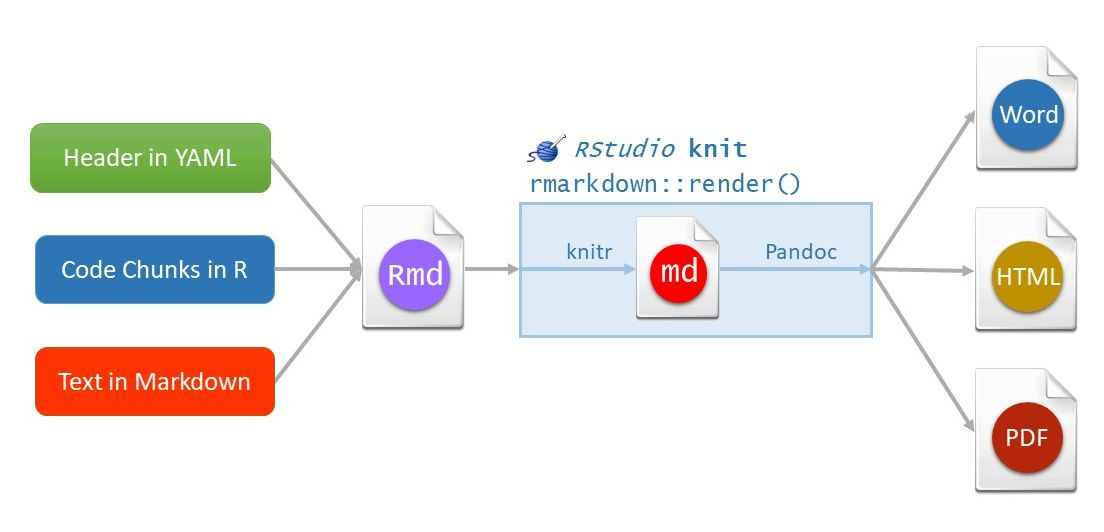
\includegraphics[width=15.33in]{image/rmarkdown} \caption{A diagram illustrating how an R Markdown document is converted to the final output document.}\label{fig:rm-pic}
\end{figure}

\hypertarget{code-chunks}{%
\section{Code Chunks}\label{code-chunks}}

To run blocks of code in RMarkdown, use code chunks. Insert a new code chunk with:

\begin{itemize}
\tightlist
\item
  \texttt{Command\ +\ Option\ +\ I} on a Mac, or \texttt{Ctrl\ +\ Alt\ +\ I} on Linux and Windows.
\item
  Another option is the ``Insert'' drop-down Icon in the toolbar and selecting R.
\end{itemize}

We recommend learning the shortcut to save time! We'll insert a new code chunk in our R Markdown Guide in a moment.

\hypertarget{running-code}{%
\subsection{Running Code}\label{running-code}}

RStudio provides many options for running code chunks in the ``Run'' drop-down tab on the toolbar.

Before running code chunks it is often a good idea to restart your R session and start with a clean environment. Do this with \texttt{Command\ +\ Shift\ +\ F10} on a Mac or \texttt{Control\ +\ Shift\ +\ F10} on Linux and Windows.

To save time, it's worth learning these shortcuts to run code:

\begin{itemize}
\tightlist
\item
  Run all chunks above the current chunk with \texttt{Command\ +\ Option\ +\ P} on a Mac, or \texttt{Ctrl\ +\ Alt\ +\ P} on Linux and Windows.
\item
  Run the current chunk with \texttt{Command\ +\ Option\ +\ C} or \texttt{Command\ +\ Shift\ +\ Enter} on a Mac. On Linux and Windows, use \texttt{Ctrl\ +\ Alt\ +\ C} or \texttt{Ctrl\ +\ Shift\ +\ Enter} to run the current chunk.
\item
  Run the next chunk with \texttt{Command\ +\ Option\ +\ N} on a Mac, or \texttt{Ctrl\ +\ Alt\ +\ N} on Linux and Windows.
\item
  Run all chunks with \texttt{Command\ +\ Option\ +\ R} or \texttt{Command\ +\ A\ +\ Enter} on a Mac. On Linux and Windows, use \texttt{Ctrl\ +\ Alt\ +\ R} or \texttt{Ctrl\ +\ A\ +\ Enter} to run all chunks.
\end{itemize}

\hypertarget{control-behavior-with-code-chunk-options}{%
\subsection{Control Behavior with Code Chunk Options}\label{control-behavior-with-code-chunk-options}}

One of the great things about R Markdown is that you have many options to control how each chunk of code is evaluated and presented. This allows you to build presentations and reports from the ground up --- including code, plots, tables, and images --- while only presenting the essential information to the intended audience. For example, you can include a plot of your results without showing the code used to generate it.

Mastering code chunk options is essential to becoming a proficient RMarkdown user. The best way to learn chunk options is to try them as you need them in your reports, so don't worry about memorizing all of this now. Here are the key chunk options to learn:

\begin{itemize}
\tightlist
\item
  \texttt{echo\ =\ FALSE}: Do not show code in the output, but run code and produce all outputs, plots, warnings and messages. The code chunk to generate a plot in the image below is an example of this.
\item
  \texttt{eval\ =\ FALSE}: Show code, but do not evaluate it.
\item
  \texttt{fig.show\ =\ "hide"}: Hide plots.
\item
  \texttt{results\ =\ "hide"}: Hides printed output.
\item
  \texttt{include\ =\ FALSE}: Run code, but suppress all output. This is helpful for setup code.
\item
  \texttt{message\ =\ FALSE}: Prevent packages from printing messages when they load. This also suppress messages generated by functions.
\item
  \texttt{warning\ =\ FALSE}: Prevent packages and functions from displaying warnings.
\end{itemize}

\hypertarget{navigating-sections-and-code-chunks}{%
\subsection{Navigating Sections and Code Chunks}\label{navigating-sections-and-code-chunks}}

Naming code chunks is useful for long documents with many chunks. With R code chunks, name the chunk like this: \texttt{\{r\ my\_boring\_chunk\_name\}}.

With named code chunks, you can navigate between chunks in the navigator included at the bottom of the R Markdown window pane. This can also make plots easy to identify by name so they can be used in other sections of your document. This navigator is also useful for quickly jumping to another section of your document.

\hypertarget{table-formatting}{%
\subsection{Table Formatting}\label{table-formatting}}

Tables in R Markdown are displayed as you see them in the R console by default. To improve the aesthetics of a table in an RMarkdown document, use the function \texttt{knitr::kable()}. Here's an example:

\begin{Shaded}
\begin{Highlighting}[]
\NormalTok{knitr}\SpecialCharTok{::}\FunctionTok{kable}\NormalTok{(}\FunctionTok{head}\NormalTok{(cars), }\AttributeTok{caption =} \StringTok{"The First Few Rows of the Cars Dataset"}\NormalTok{)}
\end{Highlighting}
\end{Shaded}

\begin{table}

\caption{\label{tab:unnamed-chunk-1}The First Few Rows of the Cars Dataset}
\centering
\begin{tabular}[t]{r|r}
\hline
speed & dist\\
\hline
4 & 2\\
\hline
4 & 10\\
\hline
7 & 4\\
\hline
7 & 22\\
\hline
8 & 16\\
\hline
9 & 10\\
\hline
\end{tabular}
\end{table}

There are \href{https://bookdown.org/yihui/rmarkdown-cookbook/table-other.html}{many other packages} for creating tables in R Markdown.

\hypertarget{inline-code}{%
\section{Inline Code}\label{inline-code}}

Directly embed R code into an R Markdown document with inline code. This is useful when you want to include information about your data in the written summary. We'll add a few examples of inline code to our R Markdown Guide to illustrate how it works.

Use inline code with \texttt{r} and add the code to evaluate within the backticks. For example, here's how we can summarize the number of rows and the number of columns in the cars dataset that's built-in to R:

\begin{verbatim}
## Inline Code

The `cars` dataset contains 50 rows and 2 columns.
\end{verbatim}

The example above highlights how it's possible to reduce errors in reports by summarizing information programmatically. If we alter the dataset and change the number of rows and columns, we only need to rerun the code for an accurate result. This is much better than trying to remember where in the document we need to update the results, determining the new numbers, and manually changing the results. RMarkdown is a powerful because it can save time and improve the quality and accuracy of reports.

\hypertarget{output-format-options}{%
\section{Output Format Options}\label{output-format-options}}

Now that we have a solid understanding about how to format an RMarkdown document, let's discuss format options. Format options that apply to the entire document are specified in the YAML header. R Markdown supports \href{https://rmarkdown.rstudio.com/authoring_quick_tour.html\#Output_Formats}{many types of output formats}.

The metadata specified in the YAML header controls the output. A single RMarkdown document can support many output formats. There are two types of output formats in the \textbf{rmarkdown} package: documents, and presentations. All available formats are listed below:

\begin{itemize}
\item
  \texttt{beamer\_presentation}
\item
  \texttt{context\_document}
\item
  \texttt{github\_document}
\item
  \texttt{html\_document}
\item
  \texttt{ioslides\_presentation}
\item
  \texttt{latex\_document}
\item
  \texttt{md\_document}
\item
  \texttt{odt\_document}
\item
  \texttt{pdf\_document}
\item
  \texttt{powerpoint\_presentation}
\item
  \texttt{rtf\_document}
\item
  \texttt{slidy\_presentation}
\item
  \texttt{word\_document}
\end{itemize}

More details in \url{https://bookdown.org/yihui/rmarkdown/documents.html\#documents} and \url{https://bookdown.org/yihui/rmarkdown/presentations.html\#presentations}. There are more output formats provided in other extension packages. For the output format names in the YAML metadata of an Rmd file, you need to include the package name if a format is from an extension package, e.g.,

\begin{verbatim}
output: tufte::tufte_html
\end{verbatim}

If the format is from the \textbf{rmarkdown} package, you do not need the \texttt{rmarkdown::} prefix (although it will not hurt).

Other packages provide even more output formats:

\begin{itemize}
\item
  The \textbf{bookdown} package, \url{https://github.com/rstudio/bookdown}, makes it easy to write books, like this one. To learn more, read \href{https://bookdown.org/yihui/bookdown/}{\emph{Authoring Books with R Markdown}}, by Yihui Xie, which is, of course, written in bookdown. Visit \href{http://www.bookdown.org/}{\textless http://www.bookdown.org\textgreater{}} to see other bookdown books written by the wider R community.
\item
  The \textbf{prettydoc} package, \url{https://github.com/yixuan/prettydoc/}, provides lightweight document formats with a range of attractive themes.
\item
  The \textbf{rticles} package, \url{https://github.com/rstudio/rticles}, compiles a selection of formats tailored for specific scientific journals.
\end{itemize}

See \url{http://rmarkdown.rstudio.com/formats.html} for a list of even more formats. Also see \href{https://www.datadreaming.org/post/r-markdown-theme-gallery/}{R Markdown Theme Gallery}.

\hypertarget{further-topics-and-links}{%
\section{Further topics and links}\label{further-topics-and-links}}

\begin{itemize}
\tightlist
\item
  Word documents
  \url{https://bookdown.org/yihui/rmarkdown-cookbook/word.html}
  \url{https://rmarkdown.rstudio.com/articles_docx.html}
\item
  Bibliography
  \url{https://bookdown.org/yihui/rmarkdown-cookbook/bibliography.html}
  \href{https://github.com/citation-style-language/styles}{Citation Style Language - Style Repository}
\item
  Cross-referencing within documents
  \url{https://bookdown.org/yihui/rmarkdown-cookbook/cross-ref.html}
\item
  Create diagrams
  \url{https://bookdown.org/yihui/rmarkdown-cookbook/diagrams.html}
\end{itemize}

\hypertarget{additional-resources}{%
\section{Additional Resources}\label{additional-resources}}

\begin{itemize}
\tightlist
\item
  \href{https://bookdown.org/yihui/rmarkdown-cookbook/}{R Markdown Cookbook}
  A comprehensive free online book that contains almost everything you need to know about RMarkdown.
\item
  \href{https://rmd4sci.njtierney.com/}{RMarkdown for Scientists}
\item
  \href{https://support.rstudio.com/hc/en-us/sections/200149716-R-Markdown}{RStudio Articles for RMarkdown}
  RStudio has published a few in-depth how to articles about using RMarkdown.
\item
  \href{https://r4ds.had.co.nz/index.html}{R for Data Science}
  Hadley Wickham provides a great overview of authoring with RMarkdown.
\item
  \href{https://bookdown.org/yihui/rmarkdown/}{R Markdown: The Definitive Guide}
  It contains a large number of technical details, it may serve you better as a reference book than a textbook.
\item
  \href{https://rmarkdown.rstudio.com/lesson-1.html}{Online lesson from RStudio}
\item
  R Markdown Cheatsheet. RStudio has published numerous cheatsheets for working with R, including a detailed cheatsheet on using R Markdown! The R Markdown cheatsheet can be accessed from within RStudio by selecting \texttt{Help\ \textgreater{}\ Cheatsheets\ \textgreater{}\ R\ Markdown\ Cheat\ Sheet}.
\end{itemize}

\hypertarget{advanced-data-manipulation}{%
\chapter{Advanced data manipulation}\label{advanced-data-manipulation}}

This chapter focuses exclusively on advanced data manipulation. I therefore assume a basic level of comfort with data manipulation.

\hypertarget{br-import}{%
\section{Importing data}\label{br-import}}

Most of the data used for analysis is found in the outside world and needs to be imported into R. Data comes in different formats.

\begin{itemize}
\item
  \textbf{Delimited text files} are the most common way of transferring data between systems in general. They are files that store tabular data using special characters (known as delimiters) to indicate rows and columns. These delimiters include commas, tabs, space, semicolons (;), pipes (\textbar), etc. The function \texttt{read.table()} is used to read delimited text files. It accepts as argument, the file path of the file and returns as output a data frame.
\item
  \textbf{Binary files} are more complex than plain text files and accessing the information in binary files requires the use of special software. Some examples of binary files that we will frequently see include Microsoft Excel spreadsheets, SAS data sets, Stata data sets, and SPSS data set. The \textbf{foreign} package contains functions that may be used to import SAS data sets and Stata data sets, and is installed by default when you install R on your computer. We can use the \textbf{readxl} package to import Microsoft Excel files, and the \textbf{haven} package to import SAS and Stata data sets. We aren't going to use these packages in this chapter. Instead, we're going to use the best \textbf{rio} package to import data in the examples below.
\end{itemize}

\begin{Shaded}
\begin{Highlighting}[]
\CommentTok{\# Description of gapminder:}
\CommentTok{\# help(gapminder, package = "gapminder")}

\CommentTok{\# importing the gapminder dataset {-} Delimited text files {-} ANSI (CP1250)}
\NormalTok{gapminder\_cp1250 }\OtherTok{\textless{}{-}} \FunctionTok{read.table}\NormalTok{(}\AttributeTok{file =} \StringTok{"data/gapminder\_ext\_CP1250.txt"}\NormalTok{, }\AttributeTok{header =}\NormalTok{ T, }\AttributeTok{sep =} \StringTok{"}\SpecialCharTok{\textbackslash{}t}\StringTok{"}\NormalTok{, }\AttributeTok{dec =} \StringTok{","}\NormalTok{, }\AttributeTok{quote =} \StringTok{"}\SpecialCharTok{\textbackslash{}"}\StringTok{"}\NormalTok{, }\AttributeTok{fileEncoding =} \StringTok{"latin2"}\NormalTok{)}

\CommentTok{\# importing the gapminder dataset {-} Delimited text files {-} UTF{-}8}
\NormalTok{gapminder\_utf8 }\OtherTok{\textless{}{-}} \FunctionTok{read.table}\NormalTok{(}\AttributeTok{file =} \StringTok{"data/gapminder\_ext\_UTF{-}8.txt"}\NormalTok{, }\AttributeTok{header =}\NormalTok{ T, }\AttributeTok{sep =} \StringTok{"}\SpecialCharTok{\textbackslash{}t}\StringTok{"}\NormalTok{, }\AttributeTok{dec =} \StringTok{","}\NormalTok{, }\AttributeTok{quote =} \StringTok{"}\SpecialCharTok{\textbackslash{}"}\StringTok{"}\NormalTok{, }\AttributeTok{fileEncoding =} \StringTok{"UTF{-}8"}\NormalTok{)}

\CommentTok{\# importing the gapminder dataset {-} Binary files}
\FunctionTok{library}\NormalTok{(rio)}
\NormalTok{gapminder\_xlsx }\OtherTok{\textless{}{-}} \FunctionTok{import}\NormalTok{(}\AttributeTok{file =} \StringTok{"data/gapminder\_ext.xlsx"}\NormalTok{)}

\CommentTok{\# checking class}
\FunctionTok{class}\NormalTok{(gapminder\_xlsx)}
\CommentTok{\#\textgreater{} [1] "data.frame"}
\end{Highlighting}
\end{Shaded}

\hypertarget{import-files-directly-from-the-web}{%
\subsection{Import files directly from the web}\label{import-files-directly-from-the-web}}

The functions \texttt{read.table()} and \texttt{rio::import()} accept a URL in the place of a dataset and downloads the dataset directly.

\begin{Shaded}
\begin{Highlighting}[]
\CommentTok{\# NCHS {-} Death rates and life expectancy at birth: }
\CommentTok{\# https://data.cdc.gov/NCHS/NCHS{-}Death{-}rates{-}and{-}life{-}expectancy{-}at{-}birth/w9j2{-}ggv5}

\CommentTok{\# storing URL}
\NormalTok{data\_url }\OtherTok{\textless{}{-}} \StringTok{\textquotesingle{}https://data.cdc.gov/api/views/w9j2{-}ggv5/rows.csv?accessType=DOWNLOAD\textquotesingle{}}

\CommentTok{\# reading in data from the URL {-} Delimited text file}
\NormalTok{life\_expectancy }\OtherTok{\textless{}{-}} \FunctionTok{read.table}\NormalTok{(data\_url, }\AttributeTok{header =}\NormalTok{ T, }\AttributeTok{sep =} \StringTok{","}\NormalTok{, }\AttributeTok{dec =} \StringTok{"."}\NormalTok{)}

\FunctionTok{head}\NormalTok{(life\_expectancy, }\DecValTok{3}\NormalTok{)}
\CommentTok{\#\textgreater{}   Year      Race        Sex Average.Life.Expectancy..Years.}
\CommentTok{\#\textgreater{} 1 1900 All Races Both Sexes                            47.3}
\CommentTok{\#\textgreater{} 2 1901 All Races Both Sexes                            49.1}
\CommentTok{\#\textgreater{} 3 1902 All Races Both Sexes                            51.5}
\CommentTok{\#\textgreater{}   Age.adjusted.Death.Rate}
\CommentTok{\#\textgreater{} 1                  2518.0}
\CommentTok{\#\textgreater{} 2                  2473.1}
\CommentTok{\#\textgreater{} 3                  2301.3}
\FunctionTok{nrow}\NormalTok{(life\_expectancy)}
\CommentTok{\#\textgreater{} [1] 1071}


\CommentTok{\# Description of Potthoff{-}Roy data: }
\CommentTok{\# help(potthoffroy, package = "mice")}

\CommentTok{\# storing URL}
\NormalTok{data\_url }\OtherTok{\textless{}{-}} \StringTok{"https://raw.github.com/abarik/rdata/master/r\_alapok/pothoff2.xlsx"}
\FunctionTok{library}\NormalTok{(rio)}
\NormalTok{pothoff }\OtherTok{\textless{}{-}} \FunctionTok{import}\NormalTok{(}\AttributeTok{file =}\NormalTok{ data\_url)}
\FunctionTok{str}\NormalTok{(pothoff)}
\CommentTok{\#\textgreater{} \textquotesingle{}data.frame\textquotesingle{}:    108 obs. of  5 variables:}
\CommentTok{\#\textgreater{}  $ person: num  1 1 1 1 2 2 2 2 3 3 ...}
\CommentTok{\#\textgreater{}  $ sex   : chr  "F" "F" "F" "F" ...}
\CommentTok{\#\textgreater{}  $ age   : num  8 10 12 14 8 10 12 14 8 10 ...}
\CommentTok{\#\textgreater{}  $ y     : num  21 20 21.5 23 21 21.5 24 25.5 20.5 24 ...}
\CommentTok{\#\textgreater{}  $ agefac: num  8 10 12 14 8 10 12 14 8 10 ...}
\end{Highlighting}
\end{Shaded}

\hypertarget{br-export}{%
\section{Exporting data}\label{br-export}}

The function \texttt{write.table()} are used to export data to delimited text file. The function \texttt{rio::export()} is used to export data to worksheets in an Excel file (or other binary file). The type of the binary file will depend on the extension given to the file name.

\begin{Shaded}
\begin{Highlighting}[]
\CommentTok{\# exporting the gapminder dataset {-} Delimited text files {-} ANSI (CP1250)}
\FunctionTok{write.table}\NormalTok{(}\AttributeTok{x =}\NormalTok{ gapminder\_xlsx, }\AttributeTok{file =} \StringTok{"output/data/gapminder\_CP1250.csv"}\NormalTok{, }\AttributeTok{quote =}\NormalTok{ F, }\AttributeTok{sep =} \StringTok{";"}\NormalTok{, }\AttributeTok{dec =} \StringTok{","}\NormalTok{, }\AttributeTok{row.names =}\NormalTok{ F, }\AttributeTok{fileEncoding =} \StringTok{"latin2"}\NormalTok{)}

\CommentTok{\# exporting the gapminder dataset {-} Delimited text files {-} UTF{-}8}
\FunctionTok{write.table}\NormalTok{(}\AttributeTok{x =}\NormalTok{ gapminder\_xlsx, }\AttributeTok{file =} \StringTok{"output/data/gapminder\_UTF{-}8.csv"}\NormalTok{, }\AttributeTok{quote =}\NormalTok{ F, }\AttributeTok{sep =} \StringTok{";"}\NormalTok{, }\AttributeTok{dec =} \StringTok{","}\NormalTok{, }\AttributeTok{row.names =}\NormalTok{ F, }\AttributeTok{fileEncoding =} \StringTok{"UTF{-}8"}\NormalTok{)}

\CommentTok{\# exporting the gapminder dataset {-} Binary files}
\FunctionTok{library}\NormalTok{(rio)}
\FunctionTok{export}\NormalTok{(}\AttributeTok{x =}\NormalTok{ gapminder\_xlsx, }\AttributeTok{file =} \StringTok{"output/data/gapminder.xlsx"}\NormalTok{, }\AttributeTok{overwrite =}\NormalTok{ T)}
\FunctionTok{export}\NormalTok{(}\AttributeTok{x =}\NormalTok{ gapminder\_xlsx, }\AttributeTok{file =} \StringTok{"output/data/gapminder.sav"}\NormalTok{)}
\end{Highlighting}
\end{Shaded}

\hypertarget{br-inspect}{%
\section{Inspecting a data frame}\label{br-inspect}}

We use the following functions to inspect a data frame:

\begin{itemize}
\tightlist
\item
  \texttt{dim()} returns dimensions
\item
  \texttt{nrow()} returns number of rows
\item
  \texttt{ncol()} returns number of columns
\item
  \texttt{str()} returns column names and their data types plus some first few values
\item
  \texttt{head()} returns the first six rows by default but can be changed using the argument \texttt{n}
\item
  \texttt{tail()} returns the last six rows by default but can be changed using the argument \texttt{n}
\end{itemize}

\begin{Shaded}
\begin{Highlighting}[]
\FunctionTok{dim}\NormalTok{(gapminder\_xlsx)}
\CommentTok{\#\textgreater{} [1] 1704    8}
\FunctionTok{nrow}\NormalTok{(gapminder\_xlsx)}
\CommentTok{\#\textgreater{} [1] 1704}
\FunctionTok{ncol}\NormalTok{(gapminder\_xlsx)}
\CommentTok{\#\textgreater{} [1] 8}
\FunctionTok{str}\NormalTok{(gapminder\_xlsx)}
\CommentTok{\#\textgreater{} \textquotesingle{}data.frame\textquotesingle{}:    1704 obs. of  8 variables:}
\CommentTok{\#\textgreater{}  $ country      : chr  "Afghanistan" "Afghanistan" "Afghanistan" "Afghanistan" ...}
\CommentTok{\#\textgreater{}  $ continent    : chr  "Asia" "Asia" "Asia" "Asia" ...}
\CommentTok{\#\textgreater{}  $ year         : num  1952 1957 1962 1967 1972 ...}
\CommentTok{\#\textgreater{}  $ lifeExp      : num  28.8 30.3 32 34 36.1 ...}
\CommentTok{\#\textgreater{}  $ pop          : num  8425333 9240934 10267083 11537966 13079460 ...}
\CommentTok{\#\textgreater{}  $ gdpPercap    : num  779 821 853 836 740 ...}
\CommentTok{\#\textgreater{}  $ country\_hun  : chr  "Afganisztán" "Afganisztán" "Afganisztán" "Afganisztán" ...}
\CommentTok{\#\textgreater{}  $ continent\_hun: chr  "Ázsia" "Ázsia" "Ázsia" "Ázsia" ...}
\FunctionTok{head}\NormalTok{(gapminder\_xlsx)}
\CommentTok{\#\textgreater{}       country continent year lifeExp      pop gdpPercap}
\CommentTok{\#\textgreater{} 1 Afghanistan      Asia 1952  28.801  8425333  779.4453}
\CommentTok{\#\textgreater{} 2 Afghanistan      Asia 1957  30.332  9240934  820.8530}
\CommentTok{\#\textgreater{} 3 Afghanistan      Asia 1962  31.997 10267083  853.1007}
\CommentTok{\#\textgreater{} 4 Afghanistan      Asia 1967  34.020 11537966  836.1971}
\CommentTok{\#\textgreater{} 5 Afghanistan      Asia 1972  36.088 13079460  739.9811}
\CommentTok{\#\textgreater{} 6 Afghanistan      Asia 1977  38.438 14880372  786.1134}
\CommentTok{\#\textgreater{}   country\_hun continent\_hun}
\CommentTok{\#\textgreater{} 1 Afganisztán         Ázsia}
\CommentTok{\#\textgreater{} 2 Afganisztán         Ázsia}
\CommentTok{\#\textgreater{} 3 Afganisztán         Ázsia}
\CommentTok{\#\textgreater{} 4 Afganisztán         Ázsia}
\CommentTok{\#\textgreater{} 5 Afganisztán         Ázsia}
\CommentTok{\#\textgreater{} 6 Afganisztán         Ázsia}
\FunctionTok{tail}\NormalTok{(gapminder\_xlsx, }\AttributeTok{n =} \DecValTok{4}\NormalTok{)}
\CommentTok{\#\textgreater{}       country continent year lifeExp      pop gdpPercap}
\CommentTok{\#\textgreater{} 1701 Zimbabwe    Africa 1992  60.377 10704340  693.4208}
\CommentTok{\#\textgreater{} 1702 Zimbabwe    Africa 1997  46.809 11404948  792.4500}
\CommentTok{\#\textgreater{} 1703 Zimbabwe    Africa 2002  39.989 11926563  672.0386}
\CommentTok{\#\textgreater{} 1704 Zimbabwe    Africa 2007  43.487 12311143  469.7093}
\CommentTok{\#\textgreater{}      country\_hun continent\_hun}
\CommentTok{\#\textgreater{} 1701    Zimbabwe        Afrika}
\CommentTok{\#\textgreater{} 1702    Zimbabwe        Afrika}
\CommentTok{\#\textgreater{} 1703    Zimbabwe        Afrika}
\CommentTok{\#\textgreater{} 1704    Zimbabwe        Afrika}
\end{Highlighting}
\end{Shaded}

\hypertarget{manipulating-columns}{%
\section{Manipulating Columns}\label{manipulating-columns}}

\hypertarget{changing-column-type}{%
\subsection{Changing column type}\label{changing-column-type}}

After importing data, column types can be changed by assigning new data types to them.

\begin{Shaded}
\begin{Highlighting}[]
\FunctionTok{str}\NormalTok{(gapminder\_xlsx)}
\CommentTok{\#\textgreater{} \textquotesingle{}data.frame\textquotesingle{}:    1704 obs. of  8 variables:}
\CommentTok{\#\textgreater{}  $ country      : chr  "Afghanistan" "Afghanistan" "Afghanistan" "Afghanistan" ...}
\CommentTok{\#\textgreater{}  $ continent    : chr  "Asia" "Asia" "Asia" "Asia" ...}
\CommentTok{\#\textgreater{}  $ year         : num  1952 1957 1962 1967 1972 ...}
\CommentTok{\#\textgreater{}  $ lifeExp      : num  28.8 30.3 32 34 36.1 ...}
\CommentTok{\#\textgreater{}  $ pop          : num  8425333 9240934 10267083 11537966 13079460 ...}
\CommentTok{\#\textgreater{}  $ gdpPercap    : num  779 821 853 836 740 ...}
\CommentTok{\#\textgreater{}  $ country\_hun  : chr  "Afganisztán" "Afganisztán" "Afganisztán" "Afganisztán" ...}
\CommentTok{\#\textgreater{}  $ continent\_hun: chr  "Ázsia" "Ázsia" "Ázsia" "Ázsia" ...}

\CommentTok{\# changing column type}
\NormalTok{gapminder\_xlsx}\SpecialCharTok{$}\NormalTok{country }\OtherTok{\textless{}{-}} \FunctionTok{factor}\NormalTok{(gapminder\_xlsx}\SpecialCharTok{$}\NormalTok{country)}
\NormalTok{gapminder\_xlsx}\SpecialCharTok{$}\NormalTok{continent }\OtherTok{\textless{}{-}} \FunctionTok{factor}\NormalTok{(gapminder\_xlsx}\SpecialCharTok{$}\NormalTok{continent)}
\NormalTok{gapminder\_xlsx}\SpecialCharTok{$}\NormalTok{country\_hun }\OtherTok{\textless{}{-}} \FunctionTok{factor}\NormalTok{(gapminder\_xlsx}\SpecialCharTok{$}\NormalTok{country\_hun)}
\NormalTok{gapminder\_xlsx}\SpecialCharTok{$}\NormalTok{continent\_hun }\OtherTok{\textless{}{-}} \FunctionTok{factor}\NormalTok{(gapminder\_xlsx}\SpecialCharTok{$}\NormalTok{continent\_hun)}

\FunctionTok{str}\NormalTok{(gapminder\_xlsx)}
\CommentTok{\#\textgreater{} \textquotesingle{}data.frame\textquotesingle{}:    1704 obs. of  8 variables:}
\CommentTok{\#\textgreater{}  $ country      : Factor w/ 142 levels "Afghanistan",..: 1 1 1 1 1 1 1 1 1 1 ...}
\CommentTok{\#\textgreater{}  $ continent    : Factor w/ 5 levels "Africa","Americas",..: 3 3 3 3 3 3 3 3 3 3 ...}
\CommentTok{\#\textgreater{}  $ year         : num  1952 1957 1962 1967 1972 ...}
\CommentTok{\#\textgreater{}  $ lifeExp      : num  28.8 30.3 32 34 36.1 ...}
\CommentTok{\#\textgreater{}  $ pop          : num  8425333 9240934 10267083 11537966 13079460 ...}
\CommentTok{\#\textgreater{}  $ gdpPercap    : num  779 821 853 836 740 ...}
\CommentTok{\#\textgreater{}  $ country\_hun  : Factor w/ 142 levels "Afganisztán",..: 1 1 1 1 1 1 1 1 1 1 ...}
\CommentTok{\#\textgreater{}  $ continent\_hun: Factor w/ 5 levels "Afrika","Amerika",..: 3 3 3 3 3 3 3 3 3 3 ...}
\end{Highlighting}
\end{Shaded}

\hypertarget{br-col-names}{%
\subsection{Renaming columns}\label{br-col-names}}

After importing data, columns can be renamed by assigning new names to them.

\begin{Shaded}
\begin{Highlighting}[]
\FunctionTok{names}\NormalTok{(gapminder\_utf8)}
\CommentTok{\#\textgreater{} [1] "country"       "continent"     "year"         }
\CommentTok{\#\textgreater{} [4] "lifeExp"       "pop"           "gdpPercap"    }
\CommentTok{\#\textgreater{} [7] "country\_hun"   "continent\_hun"}
\FunctionTok{names}\NormalTok{(gapminder\_utf8)[}\DecValTok{1}\NormalTok{] }\OtherTok{\textless{}{-}} \StringTok{"orszag"}
\FunctionTok{names}\NormalTok{(gapminder\_utf8)[}\DecValTok{2}\NormalTok{] }\OtherTok{\textless{}{-}} \StringTok{"kontinens"}
\FunctionTok{names}\NormalTok{(gapminder\_utf8)}
\CommentTok{\#\textgreater{} [1] "orszag"        "kontinens"     "year"         }
\CommentTok{\#\textgreater{} [4] "lifeExp"       "pop"           "gdpPercap"    }
\CommentTok{\#\textgreater{} [7] "country\_hun"   "continent\_hun"}

\FunctionTok{names}\NormalTok{(gapminder\_utf8)}
\CommentTok{\#\textgreater{} [1] "orszag"        "kontinens"     "year"         }
\CommentTok{\#\textgreater{} [4] "lifeExp"       "pop"           "gdpPercap"    }
\CommentTok{\#\textgreater{} [7] "country\_hun"   "continent\_hun"}
\FunctionTok{names}\NormalTok{(gapminder\_utf8)[}\DecValTok{7}\SpecialCharTok{:}\DecValTok{8}\NormalTok{] }\OtherTok{\textless{}{-}} \FunctionTok{c}\NormalTok{(}\StringTok{"orszag\_hun"}\NormalTok{, }\StringTok{"kontinens\_hun"}\NormalTok{)}
\FunctionTok{names}\NormalTok{(gapminder\_utf8)}
\CommentTok{\#\textgreater{} [1] "orszag"        "kontinens"     "year"         }
\CommentTok{\#\textgreater{} [4] "lifeExp"       "pop"           "gdpPercap"    }
\CommentTok{\#\textgreater{} [7] "orszag\_hun"    "kontinens\_hun"}
\end{Highlighting}
\end{Shaded}

\hypertarget{br-changing}{%
\subsection{Insert and derive new columns}\label{br-changing}}

\begin{Shaded}
\begin{Highlighting}[]
\CommentTok{\# Here\textquotesingle{}s a data set of 1,000 most popular movies on IMDB in the last 10 years. }
\CommentTok{\# https://www.kaggle.com/PromptCloudHQ/imdb{-}data/version/1}
\NormalTok{mov }\OtherTok{\textless{}{-}} \FunctionTok{read.table}\NormalTok{(}\AttributeTok{file =} \StringTok{"data/IMDB{-}Movie{-}Data.csv"}\NormalTok{, }\AttributeTok{header =}\NormalTok{ T, }\AttributeTok{sep =} \StringTok{","}\NormalTok{, }\AttributeTok{dec =} \StringTok{"."}\NormalTok{, }\AttributeTok{fileEncoding =} \StringTok{"UTF{-}8"}\NormalTok{, }\AttributeTok{quote =} \StringTok{"}\SpecialCharTok{\textbackslash{}"}\StringTok{"}\NormalTok{,}
                  \AttributeTok{comment.char =} \StringTok{""}\NormalTok{)}
\FunctionTok{str}\NormalTok{(mov)}
\CommentTok{\#\textgreater{} \textquotesingle{}data.frame\textquotesingle{}:    1000 obs. of  12 variables:}
\CommentTok{\#\textgreater{}  $ Rank              : int  1 2 3 4 5 6 7 8 9 10 ...}
\CommentTok{\#\textgreater{}  $ Title             : chr  "Guardians of the Galaxy" "Prometheus" "Split" "Sing" ...}
\CommentTok{\#\textgreater{}  $ Genre             : chr  "Action,Adventure,Sci{-}Fi" "Adventure,Mystery,Sci{-}Fi" "Horror,Thriller" "Animation,Comedy,Family" ...}
\CommentTok{\#\textgreater{}  $ Description       : chr  "A group of intergalactic criminals are forced to work together to stop a fanatical warrior from taking control "| \_\_truncated\_\_ "Following clues to the origin of mankind, a team finds a structure on a distant moon, but they soon realize the"| \_\_truncated\_\_ "Three girls are kidnapped by a man with a diagnosed 23 distinct personalities. They must try to escape before t"| \_\_truncated\_\_ "In a city of humanoid animals, a hustling theater impresario\textquotesingle{}s attempt to save his theater with a singing compe"| \_\_truncated\_\_ ...}
\CommentTok{\#\textgreater{}  $ Director          : chr  "James Gunn" "Ridley Scott" "M. Night Shyamalan" "Christophe Lourdelet" ...}
\CommentTok{\#\textgreater{}  $ Actors            : chr  "Chris Pratt, Vin Diesel, Bradley Cooper, Zoe Saldana" "Noomi Rapace, Logan Marshall{-}Green, Michael Fassbender, Charlize Theron" "James McAvoy, Anya Taylor{-}Joy, Haley Lu Richardson, Jessica Sula" "Matthew McConaughey,Reese Witherspoon, Seth MacFarlane, Scarlett Johansson" ...}
\CommentTok{\#\textgreater{}  $ Year              : int  2014 2012 2016 2016 2016 2016 2016 2016 2016 2016 ...}
\CommentTok{\#\textgreater{}  $ Runtime..Minutes. : int  121 124 117 108 123 103 128 89 141 116 ...}
\CommentTok{\#\textgreater{}  $ Rating            : num  8.1 7 7.3 7.2 6.2 6.1 8.3 6.4 7.1 7 ...}
\CommentTok{\#\textgreater{}  $ Votes             : int  757074 485820 157606 60545 393727 56036 258682 2490 7188 192177 ...}
\CommentTok{\#\textgreater{}  $ Revenue..Millions.: num  333 126 138 270 325 ...}
\CommentTok{\#\textgreater{}  $ Metascore         : int  76 65 62 59 40 42 93 71 78 41 ...}
\FunctionTok{names}\NormalTok{(mov) }\OtherTok{\textless{}{-}} \FunctionTok{c}\NormalTok{(}\StringTok{\textquotesingle{}Rank\textquotesingle{}}\NormalTok{, }\StringTok{\textquotesingle{}Title\textquotesingle{}}\NormalTok{, }\StringTok{\textquotesingle{}Genre\textquotesingle{}}\NormalTok{, }\StringTok{\textquotesingle{}Description\textquotesingle{}}\NormalTok{, }\StringTok{\textquotesingle{}Director\textquotesingle{}}\NormalTok{, }\StringTok{\textquotesingle{}Actors\textquotesingle{}}\NormalTok{, }\StringTok{\textquotesingle{}Year\textquotesingle{}}\NormalTok{, }
                \StringTok{\textquotesingle{}Runtime\textquotesingle{}}\NormalTok{, }\StringTok{\textquotesingle{}Rating\textquotesingle{}}\NormalTok{, }\StringTok{\textquotesingle{}Votes\textquotesingle{}}\NormalTok{, }\StringTok{\textquotesingle{}Revenue\textquotesingle{}}\NormalTok{, }\StringTok{\textquotesingle{}Metascore\textquotesingle{}}\NormalTok{)}
\end{Highlighting}
\end{Shaded}

\hypertarget{inserting-a-new-column}{%
\subsubsection{Inserting a new column}\label{inserting-a-new-column}}

To insert a new column, we index the data frame by the new column name and assign it values.

\begin{Shaded}
\begin{Highlighting}[]
\CommentTok{\# adding a new column known as example}
\NormalTok{movies }\OtherTok{\textless{}{-}}\NormalTok{ mov[,}\FunctionTok{c}\NormalTok{(}\DecValTok{2}\NormalTok{, }\DecValTok{7}\NormalTok{, }\DecValTok{11}\NormalTok{, }\DecValTok{12}\NormalTok{)]}
\FunctionTok{set.seed}\NormalTok{(}\DecValTok{123}\NormalTok{)}
\NormalTok{movies}\SpecialCharTok{$}\NormalTok{Example }\OtherTok{\textless{}{-}} \FunctionTok{sample}\NormalTok{(}\AttributeTok{x =} \DecValTok{1000}\NormalTok{)}
\FunctionTok{head}\NormalTok{(movies)}
\CommentTok{\#\textgreater{}                     Title Year Revenue Metascore Example}
\CommentTok{\#\textgreater{} 1 Guardians of the Galaxy 2014  333.13        76     415}
\CommentTok{\#\textgreater{} 2              Prometheus 2012  126.46        65     463}
\CommentTok{\#\textgreater{} 3                   Split 2016  138.12        62     179}
\CommentTok{\#\textgreater{} 4                    Sing 2016  270.32        59     526}
\CommentTok{\#\textgreater{} 5           Suicide Squad 2016  325.02        40     195}
\CommentTok{\#\textgreater{} 6          The Great Wall 2016   45.13        42     938}
\end{Highlighting}
\end{Shaded}

\hypertarget{duplicating-a-column}{%
\subsubsection{Duplicating a column}\label{duplicating-a-column}}

Duplicating a column is like inserting a new one. We simply select it and assign it a new name.

\begin{Shaded}
\begin{Highlighting}[]
\NormalTok{movies }\OtherTok{\textless{}{-}}\NormalTok{ mov[, }\FunctionTok{c}\NormalTok{(}\DecValTok{2}\NormalTok{, }\DecValTok{7}\NormalTok{, }\DecValTok{11}\NormalTok{, }\DecValTok{12}\NormalTok{)]}
\NormalTok{movies}\SpecialCharTok{$}\NormalTok{Metascore}\FloatTok{.2} \OtherTok{\textless{}{-}}\NormalTok{ movies}\SpecialCharTok{$}\NormalTok{Metascore}
\FunctionTok{head}\NormalTok{(movies)}
\CommentTok{\#\textgreater{}                     Title Year Revenue Metascore}
\CommentTok{\#\textgreater{} 1 Guardians of the Galaxy 2014  333.13        76}
\CommentTok{\#\textgreater{} 2              Prometheus 2012  126.46        65}
\CommentTok{\#\textgreater{} 3                   Split 2016  138.12        62}
\CommentTok{\#\textgreater{} 4                    Sing 2016  270.32        59}
\CommentTok{\#\textgreater{} 5           Suicide Squad 2016  325.02        40}
\CommentTok{\#\textgreater{} 6          The Great Wall 2016   45.13        42}
\CommentTok{\#\textgreater{}   Metascore.2}
\CommentTok{\#\textgreater{} 1          76}
\CommentTok{\#\textgreater{} 2          65}
\CommentTok{\#\textgreater{} 3          62}
\CommentTok{\#\textgreater{} 4          59}
\CommentTok{\#\textgreater{} 5          40}
\CommentTok{\#\textgreater{} 6          42}
\end{Highlighting}
\end{Shaded}

\hypertarget{deriving-a-new-column-from-an-existing-one}{%
\subsubsection{Deriving a new column from an existing one}\label{deriving-a-new-column-from-an-existing-one}}

\begin{Shaded}
\begin{Highlighting}[]
\NormalTok{movies }\OtherTok{\textless{}{-}}\NormalTok{ mov[, }\FunctionTok{c}\NormalTok{(}\DecValTok{2}\NormalTok{, }\DecValTok{7}\NormalTok{, }\DecValTok{9}\NormalTok{, }\DecValTok{12}\NormalTok{)]}
\NormalTok{movies}\SpecialCharTok{$}\NormalTok{Movie.Class }\OtherTok{\textless{}{-}} 
\FunctionTok{cut}\NormalTok{(movies}\SpecialCharTok{$}\NormalTok{Rating, }
    \AttributeTok{breaks =} \FunctionTok{c}\NormalTok{(}\DecValTok{0}\NormalTok{, }\FloatTok{5.5}\NormalTok{, }\FloatTok{6.5}\NormalTok{, }\DecValTok{7}\NormalTok{, }\FloatTok{7.5}\NormalTok{, }\DecValTok{10}\NormalTok{), }
    \AttributeTok{labels =} \FunctionTok{c}\NormalTok{(}\StringTok{"Very Low"}\NormalTok{, }\StringTok{"Low"}\NormalTok{, }\StringTok{"Moderate"}\NormalTok{, }\StringTok{"High"}\NormalTok{, }\StringTok{"Very High"}\NormalTok{))}
\FunctionTok{head}\NormalTok{(movies)}
\CommentTok{\#\textgreater{}                     Title Year Rating Metascore Movie.Class}
\CommentTok{\#\textgreater{} 1 Guardians of the Galaxy 2014    8.1        76   Very High}
\CommentTok{\#\textgreater{} 2              Prometheus 2012    7.0        65    Moderate}
\CommentTok{\#\textgreater{} 3                   Split 2016    7.3        62        High}
\CommentTok{\#\textgreater{} 4                    Sing 2016    7.2        59        High}
\CommentTok{\#\textgreater{} 5           Suicide Squad 2016    6.2        40         Low}
\CommentTok{\#\textgreater{} 6          The Great Wall 2016    6.1        42         Low}

\CommentTok{\# plotting the new column}
\FunctionTok{plot}\NormalTok{(movies}\SpecialCharTok{$}\NormalTok{Movie.Class)}
\end{Highlighting}
\end{Shaded}

\includegraphics{03-datamanipulation_files/figure-latex/unnamed-chunk-10-1.pdf}

\hypertarget{deriving-a-new-column-from-a-calculation}{%
\subsubsection{Deriving a new column from a calculation}\label{deriving-a-new-column-from-a-calculation}}

\begin{Shaded}
\begin{Highlighting}[]
\NormalTok{movies }\OtherTok{\textless{}{-}}\NormalTok{ mov[, }\FunctionTok{c}\NormalTok{(}\DecValTok{2}\NormalTok{, }\DecValTok{5}\NormalTok{, }\DecValTok{7}\NormalTok{, }\DecValTok{8}\NormalTok{, }\DecValTok{11}\NormalTok{)]}
\NormalTok{movies}\SpecialCharTok{$}\NormalTok{Rev.Run }\OtherTok{\textless{}{-}} \FunctionTok{round}\NormalTok{(movies}\SpecialCharTok{$}\NormalTok{Revenue}\SpecialCharTok{/}\NormalTok{movies}\SpecialCharTok{$}\NormalTok{Runtime, }\DecValTok{2}\NormalTok{)}
\FunctionTok{head}\NormalTok{(movies)}
\CommentTok{\#\textgreater{}                     Title             Director Year Runtime}
\CommentTok{\#\textgreater{} 1 Guardians of the Galaxy           James Gunn 2014     121}
\CommentTok{\#\textgreater{} 2              Prometheus         Ridley Scott 2012     124}
\CommentTok{\#\textgreater{} 3                   Split   M. Night Shyamalan 2016     117}
\CommentTok{\#\textgreater{} 4                    Sing Christophe Lourdelet 2016     108}
\CommentTok{\#\textgreater{} 5           Suicide Squad           David Ayer 2016     123}
\CommentTok{\#\textgreater{} 6          The Great Wall          Yimou Zhang 2016     103}
\CommentTok{\#\textgreater{}   Revenue Rev.Run}
\CommentTok{\#\textgreater{} 1  333.13    2.75}
\CommentTok{\#\textgreater{} 2  126.46    1.02}
\CommentTok{\#\textgreater{} 3  138.12    1.18}
\CommentTok{\#\textgreater{} 4  270.32    2.50}
\CommentTok{\#\textgreater{} 5  325.02    2.64}
\CommentTok{\#\textgreater{} 6   45.13    0.44}
\end{Highlighting}
\end{Shaded}

\hypertarget{updating-a-column}{%
\subsubsection{Updating a column}\label{updating-a-column}}

\begin{Shaded}
\begin{Highlighting}[]
\NormalTok{movies }\OtherTok{\textless{}{-}}\NormalTok{ mov[,}\FunctionTok{c}\NormalTok{(}\DecValTok{2}\NormalTok{, }\DecValTok{5}\NormalTok{, }\DecValTok{7}\NormalTok{, }\DecValTok{9}\NormalTok{, }\DecValTok{11}\NormalTok{, }\DecValTok{12}\NormalTok{)]}
\NormalTok{movies}\SpecialCharTok{$}\NormalTok{Director }\OtherTok{\textless{}{-}} \FunctionTok{toupper}\NormalTok{(movies}\SpecialCharTok{$}\NormalTok{Director)}
\NormalTok{movies}\SpecialCharTok{$}\NormalTok{Title }\OtherTok{\textless{}{-}} \FunctionTok{tolower}\NormalTok{(movies}\SpecialCharTok{$}\NormalTok{Title)}
\FunctionTok{head}\NormalTok{(movies)}
\CommentTok{\#\textgreater{}                     Title             Director Year Rating}
\CommentTok{\#\textgreater{} 1 guardians of the galaxy           JAMES GUNN 2014    8.1}
\CommentTok{\#\textgreater{} 2              prometheus         RIDLEY SCOTT 2012    7.0}
\CommentTok{\#\textgreater{} 3                   split   M. NIGHT SHYAMALAN 2016    7.3}
\CommentTok{\#\textgreater{} 4                    sing CHRISTOPHE LOURDELET 2016    7.2}
\CommentTok{\#\textgreater{} 5           suicide squad           DAVID AYER 2016    6.2}
\CommentTok{\#\textgreater{} 6          the great wall          YIMOU ZHANG 2016    6.1}
\CommentTok{\#\textgreater{}   Revenue Metascore}
\CommentTok{\#\textgreater{} 1  333.13        76}
\CommentTok{\#\textgreater{} 2  126.46        65}
\CommentTok{\#\textgreater{} 3  138.12        62}
\CommentTok{\#\textgreater{} 4  270.32        59}
\CommentTok{\#\textgreater{} 5  325.02        40}
\CommentTok{\#\textgreater{} 6   45.13        42}
\end{Highlighting}
\end{Shaded}

\hypertarget{sorting-and-ranking}{%
\subsection{Sorting and ranking}\label{sorting-and-ranking}}

\hypertarget{br-sort}{%
\subsubsection{Sorting a data frame}\label{br-sort}}

The \texttt{order()} function is used to sort a data frame. It takes a column and returns indices in ascending order. To reverse this, use \texttt{decreasing\ =\ TRUE}. Once the indices are sorted, they are used to index the data frame. The function \texttt{order()} also works on character columns as well and on multiple columns.

\begin{Shaded}
\begin{Highlighting}[]
\CommentTok{\# sorting by revenue}
\NormalTok{movies }\OtherTok{\textless{}{-}}\NormalTok{ mov[, }\FunctionTok{c}\NormalTok{(}\DecValTok{2}\NormalTok{, }\DecValTok{7}\NormalTok{, }\DecValTok{11}\NormalTok{, }\DecValTok{12}\NormalTok{)]}
\NormalTok{movies\_ordered }\OtherTok{\textless{}{-}}\NormalTok{ movies[}\FunctionTok{order}\NormalTok{(movies}\SpecialCharTok{$}\NormalTok{Revenue),]}
\FunctionTok{head}\NormalTok{(movies\_ordered)}
\CommentTok{\#\textgreater{}                Title Year Revenue Metascore}
\CommentTok{\#\textgreater{} 232 A Kind of Murder 2016    0.00        50}
\CommentTok{\#\textgreater{} 28        Dead Awake 2016    0.01        NA}
\CommentTok{\#\textgreater{} 69         Wakefield 2016    0.01        61}
\CommentTok{\#\textgreater{} 322         Lovesong 2016    0.01        74}
\CommentTok{\#\textgreater{} 678      Love, Rosie 2014    0.01        44}
\CommentTok{\#\textgreater{} 962  Into the Forest 2015    0.01        59}
\FunctionTok{tail}\NormalTok{(movies\_ordered)}
\CommentTok{\#\textgreater{}                              Title Year Revenue Metascore}
\CommentTok{\#\textgreater{} 977                    Dark Places 2015      NA        39}
\CommentTok{\#\textgreater{} 978                  Amateur Night 2016      NA        38}
\CommentTok{\#\textgreater{} 979 It\textquotesingle{}s Only the End of the World 2016      NA        48}
\CommentTok{\#\textgreater{} 989                        Martyrs 2008      NA        89}
\CommentTok{\#\textgreater{} 996           Secret in Their Eyes 2015      NA        45}
\CommentTok{\#\textgreater{} 999                   Search Party 2014      NA        22}

\CommentTok{\# sort decreasing}
\NormalTok{movies\_ordered }\OtherTok{\textless{}{-}}\NormalTok{ movies[}\FunctionTok{order}\NormalTok{(movies}\SpecialCharTok{$}\NormalTok{Revenue, }\AttributeTok{decreasing =}\NormalTok{ T),]}
\FunctionTok{head}\NormalTok{(movies\_ordered)}
\CommentTok{\#\textgreater{}                                         Title Year Revenue}
\CommentTok{\#\textgreater{} 51 Star Wars: Episode VII {-} The Force Awakens 2015  936.63}
\CommentTok{\#\textgreater{} 88                                     Avatar 2009  760.51}
\CommentTok{\#\textgreater{} 86                             Jurassic World 2015  652.18}
\CommentTok{\#\textgreater{} 77                               The Avengers 2012  623.28}
\CommentTok{\#\textgreater{} 55                            The Dark Knight 2008  533.32}
\CommentTok{\#\textgreater{} 13                                  Rogue One 2016  532.17}
\CommentTok{\#\textgreater{}    Metascore}
\CommentTok{\#\textgreater{} 51        81}
\CommentTok{\#\textgreater{} 88        83}
\CommentTok{\#\textgreater{} 86        59}
\CommentTok{\#\textgreater{} 77        69}
\CommentTok{\#\textgreater{} 55        82}
\CommentTok{\#\textgreater{} 13        65}
\FunctionTok{tail}\NormalTok{(movies\_ordered)}
\CommentTok{\#\textgreater{}                              Title Year Revenue Metascore}
\CommentTok{\#\textgreater{} 977                    Dark Places 2015      NA        39}
\CommentTok{\#\textgreater{} 978                  Amateur Night 2016      NA        38}
\CommentTok{\#\textgreater{} 979 It\textquotesingle{}s Only the End of the World 2016      NA        48}
\CommentTok{\#\textgreater{} 989                        Martyrs 2008      NA        89}
\CommentTok{\#\textgreater{} 996           Secret in Their Eyes 2015      NA        45}
\CommentTok{\#\textgreater{} 999                   Search Party 2014      NA        22}

\CommentTok{\# sort decreasing using the negative sign}
\NormalTok{movies\_ordered }\OtherTok{\textless{}{-}}\NormalTok{ movies[}\FunctionTok{order}\NormalTok{(}\SpecialCharTok{{-}}\NormalTok{movies}\SpecialCharTok{$}\NormalTok{Revenue),]}
\FunctionTok{head}\NormalTok{(movies\_ordered)}
\CommentTok{\#\textgreater{}                                         Title Year Revenue}
\CommentTok{\#\textgreater{} 51 Star Wars: Episode VII {-} The Force Awakens 2015  936.63}
\CommentTok{\#\textgreater{} 88                                     Avatar 2009  760.51}
\CommentTok{\#\textgreater{} 86                             Jurassic World 2015  652.18}
\CommentTok{\#\textgreater{} 77                               The Avengers 2012  623.28}
\CommentTok{\#\textgreater{} 55                            The Dark Knight 2008  533.32}
\CommentTok{\#\textgreater{} 13                                  Rogue One 2016  532.17}
\CommentTok{\#\textgreater{}    Metascore}
\CommentTok{\#\textgreater{} 51        81}
\CommentTok{\#\textgreater{} 88        83}
\CommentTok{\#\textgreater{} 86        59}
\CommentTok{\#\textgreater{} 77        69}
\CommentTok{\#\textgreater{} 55        82}
\CommentTok{\#\textgreater{} 13        65}
\FunctionTok{tail}\NormalTok{(movies\_ordered)}
\CommentTok{\#\textgreater{}                              Title Year Revenue Metascore}
\CommentTok{\#\textgreater{} 977                    Dark Places 2015      NA        39}
\CommentTok{\#\textgreater{} 978                  Amateur Night 2016      NA        38}
\CommentTok{\#\textgreater{} 979 It\textquotesingle{}s Only the End of the World 2016      NA        48}
\CommentTok{\#\textgreater{} 989                        Martyrs 2008      NA        89}
\CommentTok{\#\textgreater{} 996           Secret in Their Eyes 2015      NA        45}
\CommentTok{\#\textgreater{} 999                   Search Party 2014      NA        22}
\end{Highlighting}
\end{Shaded}

By default, \texttt{NA} values appear at the end of the sorted column, but this can be changed by setting \texttt{na.last\ =\ FALSE} so that they appear first.

\begin{Shaded}
\begin{Highlighting}[]
\CommentTok{\# placing NA at the beginning}
\NormalTok{movies\_ordered }\OtherTok{\textless{}{-}}\NormalTok{ movies[}\FunctionTok{order}\NormalTok{(movies}\SpecialCharTok{$}\NormalTok{Revenue, }\AttributeTok{na.last =} \ConstantTok{FALSE}\NormalTok{),]}
\FunctionTok{head}\NormalTok{(movies\_ordered)}
\CommentTok{\#\textgreater{}                      Title Year Revenue Metascore}
\CommentTok{\#\textgreater{} 8                 Mindhorn 2016      NA        71}
\CommentTok{\#\textgreater{} 23          Hounds of Love 2016      NA        72}
\CommentTok{\#\textgreater{} 26         Paris pieds nus 2016      NA        NA}
\CommentTok{\#\textgreater{} 40               5{-} 25{-} 77 2007      NA        NA}
\CommentTok{\#\textgreater{} 43 Don\textquotesingle{}t Fuck in the Woods 2016      NA        NA}
\CommentTok{\#\textgreater{} 48                  Fallen 2016      NA        NA}
\FunctionTok{tail}\NormalTok{(movies\_ordered)}
\CommentTok{\#\textgreater{}                                         Title Year Revenue}
\CommentTok{\#\textgreater{} 13                                  Rogue One 2016  532.17}
\CommentTok{\#\textgreater{} 55                            The Dark Knight 2008  533.32}
\CommentTok{\#\textgreater{} 77                               The Avengers 2012  623.28}
\CommentTok{\#\textgreater{} 86                             Jurassic World 2015  652.18}
\CommentTok{\#\textgreater{} 88                                     Avatar 2009  760.51}
\CommentTok{\#\textgreater{} 51 Star Wars: Episode VII {-} The Force Awakens 2015  936.63}
\CommentTok{\#\textgreater{}    Metascore}
\CommentTok{\#\textgreater{} 13        65}
\CommentTok{\#\textgreater{} 55        82}
\CommentTok{\#\textgreater{} 77        69}
\CommentTok{\#\textgreater{} 86        59}
\CommentTok{\#\textgreater{} 88        83}
\CommentTok{\#\textgreater{} 51        81}

\CommentTok{\# sorting on multiple columns}
\NormalTok{movies\_ordered }\OtherTok{\textless{}{-}}\NormalTok{ movies[}\FunctionTok{order}\NormalTok{(movies}\SpecialCharTok{$}\NormalTok{Metascore, movies}\SpecialCharTok{$}\NormalTok{Revenue, }\AttributeTok{decreasing =}\NormalTok{ T),]}
\FunctionTok{head}\NormalTok{(movies\_ordered, }\DecValTok{10}\NormalTok{)}
\CommentTok{\#\textgreater{}                     Title Year Revenue Metascore}
\CommentTok{\#\textgreater{} 657               Boyhood 2014   25.36       100}
\CommentTok{\#\textgreater{} 42              Moonlight 2016   27.85        99}
\CommentTok{\#\textgreater{} 231       Pan\textquotesingle{}s Labyrinth 2006   37.62        98}
\CommentTok{\#\textgreater{} 510               Gravity 2013  274.08        96}
\CommentTok{\#\textgreater{} 490           Ratatouille 2007  206.44        96}
\CommentTok{\#\textgreater{} 112      12 Years a Slave 2013   56.67        96}
\CommentTok{\#\textgreater{} 22  Manchester by the Sea 2016   47.70        96}
\CommentTok{\#\textgreater{} 325    The Social Network 2010   96.92        95}
\CommentTok{\#\textgreater{} 407      Zero Dark Thirty 2012   95.72        95}
\CommentTok{\#\textgreater{} 502                 Carol 2015    0.25        95}
\end{Highlighting}
\end{Shaded}

\hypertarget{ranking}{%
\subsubsection{Ranking}\label{ranking}}

The function \texttt{rank()} ranks column values. It does this in ascending order but can be reversed by placing a negative sign in front of the ranking column as there is no decreasing argument here as was the case with the \texttt{order()} function.

\begin{Shaded}
\begin{Highlighting}[]
\CommentTok{\# returning ranks by revenue}
\FunctionTok{rank}\NormalTok{(movies}\SpecialCharTok{$}\NormalTok{Revenue)[}\DecValTok{1}\SpecialCharTok{:}\DecValTok{10}\NormalTok{]}
\CommentTok{\#\textgreater{}  [1] 841 678 702 819 839 419 724 873 182 623}

\CommentTok{\# adding a rank to the data frame}
\NormalTok{movies }\OtherTok{\textless{}{-}}\NormalTok{ mov[, }\FunctionTok{c}\NormalTok{(}\DecValTok{2}\NormalTok{, }\DecValTok{7}\NormalTok{, }\DecValTok{11}\NormalTok{, }\DecValTok{12}\NormalTok{)]}
\NormalTok{movies}\SpecialCharTok{$}\NormalTok{Ranking }\OtherTok{\textless{}{-}} \FunctionTok{rank}\NormalTok{(movies}\SpecialCharTok{$}\NormalTok{Revenue)}
\FunctionTok{head}\NormalTok{(movies)}
\CommentTok{\#\textgreater{}                     Title Year Revenue Metascore Ranking}
\CommentTok{\#\textgreater{} 1 Guardians of the Galaxy 2014  333.13        76     841}
\CommentTok{\#\textgreater{} 2              Prometheus 2012  126.46        65     678}
\CommentTok{\#\textgreater{} 3                   Split 2016  138.12        62     702}
\CommentTok{\#\textgreater{} 4                    Sing 2016  270.32        59     819}
\CommentTok{\#\textgreater{} 5           Suicide Squad 2016  325.02        40     839}
\CommentTok{\#\textgreater{} 6          The Great Wall 2016   45.13        42     419}

\CommentTok{\# sorting by rank}
\NormalTok{movies }\OtherTok{\textless{}{-}}\NormalTok{ mov[, }\FunctionTok{c}\NormalTok{(}\DecValTok{2}\NormalTok{, }\DecValTok{7}\NormalTok{, }\DecValTok{11}\NormalTok{, }\DecValTok{12}\NormalTok{)]}
\NormalTok{movies}\SpecialCharTok{$}\NormalTok{Ranking }\OtherTok{\textless{}{-}} \FunctionTok{rank}\NormalTok{(movies}\SpecialCharTok{$}\NormalTok{Revenue)}
\NormalTok{movies }\OtherTok{\textless{}{-}}\NormalTok{ movies[}\FunctionTok{order}\NormalTok{(movies}\SpecialCharTok{$}\NormalTok{Ranking), ]}
\FunctionTok{head}\NormalTok{(movies)}
\CommentTok{\#\textgreater{}                Title Year Revenue Metascore Ranking}
\CommentTok{\#\textgreater{} 232 A Kind of Murder 2016    0.00        50       1}
\CommentTok{\#\textgreater{} 28        Dead Awake 2016    0.01        NA       4}
\CommentTok{\#\textgreater{} 69         Wakefield 2016    0.01        61       4}
\CommentTok{\#\textgreater{} 322         Lovesong 2016    0.01        74       4}
\CommentTok{\#\textgreater{} 678      Love, Rosie 2014    0.01        44       4}
\CommentTok{\#\textgreater{} 962  Into the Forest 2015    0.01        59       4}

\CommentTok{\# placing NA values at the beginning}
\NormalTok{movies }\OtherTok{\textless{}{-}}\NormalTok{ mov[, }\FunctionTok{c}\NormalTok{(}\DecValTok{2}\NormalTok{, }\DecValTok{7}\NormalTok{, }\DecValTok{11}\NormalTok{, }\DecValTok{12}\NormalTok{)]}
\NormalTok{movies}\SpecialCharTok{$}\NormalTok{Ranking }\OtherTok{\textless{}{-}} \FunctionTok{rank}\NormalTok{(movies}\SpecialCharTok{$}\NormalTok{Revenue, }\AttributeTok{na.last =}\NormalTok{ F)}
\NormalTok{movies }\OtherTok{\textless{}{-}}\NormalTok{ movies[}\FunctionTok{order}\NormalTok{(movies}\SpecialCharTok{$}\NormalTok{Ranking), ]}
\FunctionTok{head}\NormalTok{(movies)}
\CommentTok{\#\textgreater{}                      Title Year Revenue Metascore Ranking}
\CommentTok{\#\textgreater{} 8                 Mindhorn 2016      NA        71       1}
\CommentTok{\#\textgreater{} 23          Hounds of Love 2016      NA        72       2}
\CommentTok{\#\textgreater{} 26         Paris pieds nus 2016      NA        NA       3}
\CommentTok{\#\textgreater{} 40               5{-} 25{-} 77 2007      NA        NA       4}
\CommentTok{\#\textgreater{} 43 Don\textquotesingle{}t Fuck in the Woods 2016      NA        NA       5}
\CommentTok{\#\textgreater{} 48                  Fallen 2016      NA        NA       6}
\end{Highlighting}
\end{Shaded}

There is no decreasing argument with \texttt{rank()}, hence our only chance of performing a decreasing rank is to use the negative sign.

\begin{Shaded}
\begin{Highlighting}[]
\CommentTok{\# performing a decreasing rank}
\NormalTok{movies }\OtherTok{\textless{}{-}}\NormalTok{ mov[, }\FunctionTok{c}\NormalTok{(}\DecValTok{2}\NormalTok{, }\DecValTok{7}\NormalTok{, }\DecValTok{8}\NormalTok{, }\DecValTok{11}\NormalTok{)]}
\NormalTok{movies}\SpecialCharTok{$}\NormalTok{Ranking }\OtherTok{\textless{}{-}} \FunctionTok{rank}\NormalTok{(}\SpecialCharTok{{-}}\NormalTok{movies}\SpecialCharTok{$}\NormalTok{Revenue)}
\NormalTok{movies }\OtherTok{\textless{}{-}}\NormalTok{ movies[}\FunctionTok{order}\NormalTok{(movies}\SpecialCharTok{$}\NormalTok{Ranking), ]}
\FunctionTok{head}\NormalTok{(movies)}
\CommentTok{\#\textgreater{}                                         Title Year Runtime}
\CommentTok{\#\textgreater{} 51 Star Wars: Episode VII {-} The Force Awakens 2015     136}
\CommentTok{\#\textgreater{} 88                                     Avatar 2009     162}
\CommentTok{\#\textgreater{} 86                             Jurassic World 2015     124}
\CommentTok{\#\textgreater{} 77                               The Avengers 2012     143}
\CommentTok{\#\textgreater{} 55                            The Dark Knight 2008     152}
\CommentTok{\#\textgreater{} 13                                  Rogue One 2016     133}
\CommentTok{\#\textgreater{}    Revenue Ranking}
\CommentTok{\#\textgreater{} 51  936.63       1}
\CommentTok{\#\textgreater{} 88  760.51       2}
\CommentTok{\#\textgreater{} 86  652.18       3}
\CommentTok{\#\textgreater{} 77  623.28       4}
\CommentTok{\#\textgreater{} 55  533.32       5}
\CommentTok{\#\textgreater{} 13  532.17       6}
\end{Highlighting}
\end{Shaded}

\hypertarget{splitting-and-merging-columns}{%
\subsection{Splitting and Merging columns}\label{splitting-and-merging-columns}}

\hypertarget{splitting-columns}{%
\subsubsection{Splitting columns}\label{splitting-columns}}

To split a data frame, we do the following

\begin{itemize}
\tightlist
\item
  select the column concerned and pass it to the function \texttt{strsplit()} together with the string to split on. This will return a list
\item
  using the function \texttt{do.call(\textquotesingle{}rbind\textquotesingle{},\ dfs)} convert the list to a data frame
\item
  rename the columns of the new data frame
\item
  finally using \texttt{cbind()}, combine the new data frame to the original one
\end{itemize}

\begin{Shaded}
\begin{Highlighting}[]
\CommentTok{\# Airports are ranked by travellers and experts based on various measures.}
\CommentTok{\# https://www.kaggle.com/jonahmary17/airports}

\CommentTok{\# reading data}
\NormalTok{busiestAirports }\OtherTok{\textless{}{-}} \FunctionTok{read.table}\NormalTok{(}\AttributeTok{file =} \StringTok{"data/busiestAirports.csv"}\NormalTok{, }
                              \AttributeTok{header =}\NormalTok{ T, }
                              \AttributeTok{sep=}\StringTok{","}\NormalTok{, }
                              \AttributeTok{dec =} \StringTok{"."}\NormalTok{, }
                              \AttributeTok{quote =} \StringTok{"}\SpecialCharTok{\textbackslash{}"}\StringTok{"}\NormalTok{)}

\NormalTok{busiestAirports }\OtherTok{\textless{}{-}}\NormalTok{ busiestAirports[}\SpecialCharTok{{-}}\FunctionTok{c}\NormalTok{(}\DecValTok{1}\NormalTok{, }\DecValTok{2}\NormalTok{, }\DecValTok{3}\NormalTok{, }\DecValTok{4}\NormalTok{, }\DecValTok{8}\NormalTok{)]}
\FunctionTok{head}\NormalTok{(busiestAirports, }\DecValTok{3}\NormalTok{)}
\CommentTok{\#\textgreater{}   code.iata.icao.                 location}
\CommentTok{\#\textgreater{} 1        ATL/KATL         Atlanta, Georgia}
\CommentTok{\#\textgreater{} 2        PEK/ZBAA Chaoyang{-}Shunyi, Beijing}
\CommentTok{\#\textgreater{} 3        DXB/OMDB           Garhoud, Dubai}
\CommentTok{\#\textgreater{}                country}
\CommentTok{\#\textgreater{} 1        United States}
\CommentTok{\#\textgreater{} 2                China}
\CommentTok{\#\textgreater{} 3 United Arab Emirates}

\CommentTok{\# splitting column}
\FunctionTok{strsplit}\NormalTok{(busiestAirports}\SpecialCharTok{$}\NormalTok{code.iata.icao.,}\StringTok{\textquotesingle{}/\textquotesingle{}}\NormalTok{)[}\DecValTok{1}\SpecialCharTok{:}\DecValTok{3}\NormalTok{]}
\CommentTok{\#\textgreater{} [[1]]}
\CommentTok{\#\textgreater{} [1] "ATL"  "KATL"}
\CommentTok{\#\textgreater{} }
\CommentTok{\#\textgreater{} [[2]]}
\CommentTok{\#\textgreater{} [1] "PEK"  "ZBAA"}
\CommentTok{\#\textgreater{} }
\CommentTok{\#\textgreater{} [[3]]}
\CommentTok{\#\textgreater{} [1] "DXB"  "OMDB"}

\CommentTok{\# converting to a data frame}
\NormalTok{iata\_icao }\OtherTok{\textless{}{-}} 
\FunctionTok{data.frame}\NormalTok{(}\FunctionTok{do.call}\NormalTok{(}\StringTok{\textquotesingle{}rbind\textquotesingle{}}\NormalTok{, }\FunctionTok{strsplit}\NormalTok{(busiestAirports}\SpecialCharTok{$}\NormalTok{code.iata.icao., }\StringTok{\textquotesingle{}/\textquotesingle{}}\NormalTok{)))}
\FunctionTok{head}\NormalTok{(iata\_icao, }\DecValTok{3}\NormalTok{)}
\CommentTok{\#\textgreater{}    X1   X2}
\CommentTok{\#\textgreater{} 1 ATL KATL}
\CommentTok{\#\textgreater{} 2 PEK ZBAA}
\CommentTok{\#\textgreater{} 3 DXB OMDB}

\CommentTok{\# renaming columns}
\FunctionTok{names}\NormalTok{(iata\_icao) }\OtherTok{\textless{}{-}} \FunctionTok{c}\NormalTok{(}\StringTok{\textquotesingle{}iata\textquotesingle{}}\NormalTok{, }\StringTok{\textquotesingle{}icao\textquotesingle{}}\NormalTok{)}
\FunctionTok{head}\NormalTok{(iata\_icao, }\DecValTok{3}\NormalTok{)}
\CommentTok{\#\textgreater{}   iata icao}
\CommentTok{\#\textgreater{} 1  ATL KATL}
\CommentTok{\#\textgreater{} 2  PEK ZBAA}
\CommentTok{\#\textgreater{} 3  DXB OMDB}

\CommentTok{\# combining both data frames}
\NormalTok{busiest\_Airports }\OtherTok{\textless{}{-}} \FunctionTok{cbind}\NormalTok{(busiestAirports[}\SpecialCharTok{{-}}\DecValTok{1}\NormalTok{], iata\_icao)}
\FunctionTok{head}\NormalTok{(busiest\_Airports)}
\CommentTok{\#\textgreater{}                   location              country iata icao}
\CommentTok{\#\textgreater{} 1         Atlanta, Georgia        United States  ATL KATL}
\CommentTok{\#\textgreater{} 2 Chaoyang{-}Shunyi, Beijing                China  PEK ZBAA}
\CommentTok{\#\textgreater{} 3           Garhoud, Dubai United Arab Emirates  DXB OMDB}
\CommentTok{\#\textgreater{} 4  Los Angeles, California        United States  LAX KLAX}
\CommentTok{\#\textgreater{} 5               Ota, Tokyo                Japan  HND RJTT}
\CommentTok{\#\textgreater{} 6        Chicago, Illinois        United States  ORD KORD}
\end{Highlighting}
\end{Shaded}

\hypertarget{merging-columns}{%
\subsubsection{Merging columns}\label{merging-columns}}

The function \texttt{paste()} is used to merge columns.

\begin{Shaded}
\begin{Highlighting}[]
\CommentTok{\# merging iata and icao into iata\_icao}
\NormalTok{busiest\_Airports}\SpecialCharTok{$}\NormalTok{iata\_icao }\OtherTok{\textless{}{-}} 
\FunctionTok{paste}\NormalTok{(busiest\_Airports}\SpecialCharTok{$}\NormalTok{iata, busiest\_Airports}\SpecialCharTok{$}\NormalTok{icao, }\AttributeTok{sep =} \StringTok{\textquotesingle{}{-}\textquotesingle{}}\NormalTok{)}
\FunctionTok{head}\NormalTok{(busiest\_Airports)}
\CommentTok{\#\textgreater{}                   location              country iata icao}
\CommentTok{\#\textgreater{} 1         Atlanta, Georgia        United States  ATL KATL}
\CommentTok{\#\textgreater{} 2 Chaoyang{-}Shunyi, Beijing                China  PEK ZBAA}
\CommentTok{\#\textgreater{} 3           Garhoud, Dubai United Arab Emirates  DXB OMDB}
\CommentTok{\#\textgreater{} 4  Los Angeles, California        United States  LAX KLAX}
\CommentTok{\#\textgreater{} 5               Ota, Tokyo                Japan  HND RJTT}
\CommentTok{\#\textgreater{} 6        Chicago, Illinois        United States  ORD KORD}
\CommentTok{\#\textgreater{}   iata\_icao}
\CommentTok{\#\textgreater{} 1  ATL{-}KATL}
\CommentTok{\#\textgreater{} 2  PEK{-}ZBAA}
\CommentTok{\#\textgreater{} 3  DXB{-}OMDB}
\CommentTok{\#\textgreater{} 4  LAX{-}KLAX}
\CommentTok{\#\textgreater{} 5  HND{-}RJTT}
\CommentTok{\#\textgreater{} 6  ORD{-}KORD}
\end{Highlighting}
\end{Shaded}

\hypertarget{br-filter-cols}{%
\section{Selecting columns}\label{br-filter-cols}}

The function \texttt{subset()} or \texttt{{[}} is used to select columns.

\begin{Shaded}
\begin{Highlighting}[]
\FunctionTok{head}\NormalTok{(gapminder\_cp1250[, }\FunctionTok{c}\NormalTok{(}\DecValTok{1}\NormalTok{, }\DecValTok{3}\NormalTok{)])}
\CommentTok{\#\textgreater{}       country year}
\CommentTok{\#\textgreater{} 1 Afghanistan 1952}
\CommentTok{\#\textgreater{} 2 Afghanistan 1957}
\CommentTok{\#\textgreater{} 3 Afghanistan 1962}
\CommentTok{\#\textgreater{} 4 Afghanistan 1967}
\CommentTok{\#\textgreater{} 5 Afghanistan 1972}
\CommentTok{\#\textgreater{} 6 Afghanistan 1977}
\FunctionTok{head}\NormalTok{(gapminder\_cp1250[, }\FunctionTok{c}\NormalTok{(}\StringTok{"country"}\NormalTok{, }\StringTok{"gdpPercap"}\NormalTok{)])}
\CommentTok{\#\textgreater{}       country gdpPercap}
\CommentTok{\#\textgreater{} 1 Afghanistan  779.4453}
\CommentTok{\#\textgreater{} 2 Afghanistan  820.8530}
\CommentTok{\#\textgreater{} 3 Afghanistan  853.1007}
\CommentTok{\#\textgreater{} 4 Afghanistan  836.1971}
\CommentTok{\#\textgreater{} 5 Afghanistan  739.9811}
\CommentTok{\#\textgreater{} 6 Afghanistan  786.1134}
\FunctionTok{head}\NormalTok{(}\FunctionTok{subset}\NormalTok{(gapminder\_cp1250, }\AttributeTok{select =} \FunctionTok{c}\NormalTok{(}\StringTok{"country"}\NormalTok{, }\StringTok{"gdpPercap"}\NormalTok{)))}
\CommentTok{\#\textgreater{}       country gdpPercap}
\CommentTok{\#\textgreater{} 1 Afghanistan  779.4453}
\CommentTok{\#\textgreater{} 2 Afghanistan  820.8530}
\CommentTok{\#\textgreater{} 3 Afghanistan  853.1007}
\CommentTok{\#\textgreater{} 4 Afghanistan  836.1971}
\CommentTok{\#\textgreater{} 5 Afghanistan  739.9811}
\CommentTok{\#\textgreater{} 6 Afghanistan  786.1134}
\end{Highlighting}
\end{Shaded}

\hypertarget{deleting-columns}{%
\section{Deleting columns}\label{deleting-columns}}

There is no special function to delete columns but \texttt{{[}} and \texttt{NULL} can be used to drop unwanted columns.

\begin{Shaded}
\begin{Highlighting}[]
\FunctionTok{str}\NormalTok{(gapminder\_cp1250)}
\CommentTok{\#\textgreater{} \textquotesingle{}data.frame\textquotesingle{}:    1704 obs. of  8 variables:}
\CommentTok{\#\textgreater{}  $ country      : chr  "Afghanistan" "Afghanistan" "Afghanistan" "Afghanistan" ...}
\CommentTok{\#\textgreater{}  $ continent    : chr  "Asia" "Asia" "Asia" "Asia" ...}
\CommentTok{\#\textgreater{}  $ year         : int  1952 1957 1962 1967 1972 1977 1982 1987 1992 1997 ...}
\CommentTok{\#\textgreater{}  $ lifeExp      : num  28.8 30.3 32 34 36.1 ...}
\CommentTok{\#\textgreater{}  $ pop          : int  8425333 9240934 10267083 11537966 13079460 14880372 12881816 13867957 16317921 22227415 ...}
\CommentTok{\#\textgreater{}  $ gdpPercap    : num  779 821 853 836 740 ...}
\CommentTok{\#\textgreater{}  $ country\_hun  : chr  "Afganisztán" "Afganisztán" "Afganisztán" "Afganisztán" ...}
\CommentTok{\#\textgreater{}  $ continent\_hun: chr  "Ázsia" "Ázsia" "Ázsia" "Ázsia" ...}
\NormalTok{gapminder\_cp1250}\SpecialCharTok{$}\NormalTok{pop }\OtherTok{\textless{}{-}} \ConstantTok{NULL}
\FunctionTok{str}\NormalTok{(gapminder\_cp1250)}
\CommentTok{\#\textgreater{} \textquotesingle{}data.frame\textquotesingle{}:    1704 obs. of  7 variables:}
\CommentTok{\#\textgreater{}  $ country      : chr  "Afghanistan" "Afghanistan" "Afghanistan" "Afghanistan" ...}
\CommentTok{\#\textgreater{}  $ continent    : chr  "Asia" "Asia" "Asia" "Asia" ...}
\CommentTok{\#\textgreater{}  $ year         : int  1952 1957 1962 1967 1972 1977 1982 1987 1992 1997 ...}
\CommentTok{\#\textgreater{}  $ lifeExp      : num  28.8 30.3 32 34 36.1 ...}
\CommentTok{\#\textgreater{}  $ gdpPercap    : num  779 821 853 836 740 ...}
\CommentTok{\#\textgreater{}  $ country\_hun  : chr  "Afganisztán" "Afganisztán" "Afganisztán" "Afganisztán" ...}
\CommentTok{\#\textgreater{}  $ continent\_hun: chr  "Ázsia" "Ázsia" "Ázsia" "Ázsia" ...}

\FunctionTok{str}\NormalTok{(gapminder\_cp1250)}
\CommentTok{\#\textgreater{} \textquotesingle{}data.frame\textquotesingle{}:    1704 obs. of  7 variables:}
\CommentTok{\#\textgreater{}  $ country      : chr  "Afghanistan" "Afghanistan" "Afghanistan" "Afghanistan" ...}
\CommentTok{\#\textgreater{}  $ continent    : chr  "Asia" "Asia" "Asia" "Asia" ...}
\CommentTok{\#\textgreater{}  $ year         : int  1952 1957 1962 1967 1972 1977 1982 1987 1992 1997 ...}
\CommentTok{\#\textgreater{}  $ lifeExp      : num  28.8 30.3 32 34 36.1 ...}
\CommentTok{\#\textgreater{}  $ gdpPercap    : num  779 821 853 836 740 ...}
\CommentTok{\#\textgreater{}  $ country\_hun  : chr  "Afganisztán" "Afganisztán" "Afganisztán" "Afganisztán" ...}
\CommentTok{\#\textgreater{}  $ continent\_hun: chr  "Ázsia" "Ázsia" "Ázsia" "Ázsia" ...}
\NormalTok{gapminder\_cp1250 }\OtherTok{\textless{}{-}}\NormalTok{ gapminder\_cp1250[, }\FunctionTok{c}\NormalTok{(}\DecValTok{1}\NormalTok{, }\DecValTok{2}\NormalTok{, }\DecValTok{5}\NormalTok{, }\DecValTok{6}\NormalTok{)]}
\FunctionTok{str}\NormalTok{(gapminder\_cp1250)}
\CommentTok{\#\textgreater{} \textquotesingle{}data.frame\textquotesingle{}:    1704 obs. of  4 variables:}
\CommentTok{\#\textgreater{}  $ country    : chr  "Afghanistan" "Afghanistan" "Afghanistan" "Afghanistan" ...}
\CommentTok{\#\textgreater{}  $ continent  : chr  "Asia" "Asia" "Asia" "Asia" ...}
\CommentTok{\#\textgreater{}  $ gdpPercap  : num  779 821 853 836 740 ...}
\CommentTok{\#\textgreater{}  $ country\_hun: chr  "Afganisztán" "Afganisztán" "Afganisztán" "Afganisztán" ...}
\end{Highlighting}
\end{Shaded}

\hypertarget{manipulating-rows}{%
\section{Manipulating Rows}\label{manipulating-rows}}

\hypertarget{br-row-names}{%
\subsection{Renaming rows}\label{br-row-names}}

After importing data, rows can be renamed by assigning new names to them.

\begin{Shaded}
\begin{Highlighting}[]
\FunctionTok{rownames}\NormalTok{(gapminder\_utf8)[}\DecValTok{1}\SpecialCharTok{:}\DecValTok{6}\NormalTok{]}
\CommentTok{\#\textgreater{} [1] "1" "2" "3" "4" "5" "6"}
\FunctionTok{rownames}\NormalTok{(gapminder\_utf8) }\OtherTok{\textless{}{-}} \FunctionTok{paste0}\NormalTok{(}\StringTok{"RN{-}"}\NormalTok{, }\DecValTok{1}\SpecialCharTok{:}\FunctionTok{nrow}\NormalTok{(gapminder\_utf8))}
\FunctionTok{head}\NormalTok{(gapminder\_utf8)}
\CommentTok{\#\textgreater{}           orszag kontinens year lifeExp      pop gdpPercap}
\CommentTok{\#\textgreater{} RN{-}1 Afghanistan      Asia 1952  28.801  8425333  779.4453}
\CommentTok{\#\textgreater{} RN{-}2 Afghanistan      Asia 1957  30.332  9240934  820.8530}
\CommentTok{\#\textgreater{} RN{-}3 Afghanistan      Asia 1962  31.997 10267083  853.1007}
\CommentTok{\#\textgreater{} RN{-}4 Afghanistan      Asia 1967  34.020 11537966  836.1971}
\CommentTok{\#\textgreater{} RN{-}5 Afghanistan      Asia 1972  36.088 13079460  739.9811}
\CommentTok{\#\textgreater{} RN{-}6 Afghanistan      Asia 1977  38.438 14880372  786.1134}
\CommentTok{\#\textgreater{}       orszag\_hun kontinens\_hun}
\CommentTok{\#\textgreater{} RN{-}1 Afganisztán         Ázsia}
\CommentTok{\#\textgreater{} RN{-}2 Afganisztán         Ázsia}
\CommentTok{\#\textgreater{} RN{-}3 Afganisztán         Ázsia}
\CommentTok{\#\textgreater{} RN{-}4 Afganisztán         Ázsia}
\CommentTok{\#\textgreater{} RN{-}5 Afganisztán         Ázsia}
\CommentTok{\#\textgreater{} RN{-}6 Afganisztán         Ázsia}
\FunctionTok{rownames}\NormalTok{(gapminder\_utf8) }\OtherTok{\textless{}{-}} \DecValTok{1}\SpecialCharTok{:}\FunctionTok{nrow}\NormalTok{(gapminder\_utf8) }\CommentTok{\# reset row names}
\FunctionTok{head}\NormalTok{(gapminder\_utf8)}
\CommentTok{\#\textgreater{}        orszag kontinens year lifeExp      pop gdpPercap}
\CommentTok{\#\textgreater{} 1 Afghanistan      Asia 1952  28.801  8425333  779.4453}
\CommentTok{\#\textgreater{} 2 Afghanistan      Asia 1957  30.332  9240934  820.8530}
\CommentTok{\#\textgreater{} 3 Afghanistan      Asia 1962  31.997 10267083  853.1007}
\CommentTok{\#\textgreater{} 4 Afghanistan      Asia 1967  34.020 11537966  836.1971}
\CommentTok{\#\textgreater{} 5 Afghanistan      Asia 1972  36.088 13079460  739.9811}
\CommentTok{\#\textgreater{} 6 Afghanistan      Asia 1977  38.438 14880372  786.1134}
\CommentTok{\#\textgreater{}    orszag\_hun kontinens\_hun}
\CommentTok{\#\textgreater{} 1 Afganisztán         Ázsia}
\CommentTok{\#\textgreater{} 2 Afganisztán         Ázsia}
\CommentTok{\#\textgreater{} 3 Afganisztán         Ázsia}
\CommentTok{\#\textgreater{} 4 Afganisztán         Ázsia}
\CommentTok{\#\textgreater{} 5 Afganisztán         Ázsia}
\CommentTok{\#\textgreater{} 6 Afganisztán         Ázsia}
\end{Highlighting}
\end{Shaded}

\hypertarget{adding-rows}{%
\subsection{Adding rows}\label{adding-rows}}

\hypertarget{adding-rows-by-assignment}{%
\subsubsection{Adding rows by assignment}\label{adding-rows-by-assignment}}

\begin{Shaded}
\begin{Highlighting}[]
\NormalTok{movies }\OtherTok{\textless{}{-}}\NormalTok{ mov[, }\FunctionTok{c}\NormalTok{(}\DecValTok{2}\NormalTok{, }\DecValTok{5}\NormalTok{, }\DecValTok{7}\NormalTok{, }\DecValTok{9}\NormalTok{, }\DecValTok{11}\NormalTok{, }\DecValTok{12}\NormalTok{)]}
\FunctionTok{tail}\NormalTok{(movies, }\DecValTok{3}\NormalTok{)}
\CommentTok{\#\textgreater{}                       Title         Director Year Rating}
\CommentTok{\#\textgreater{} 998  Step Up 2: The Streets       Jon M. Chu 2008    6.2}
\CommentTok{\#\textgreater{} 999            Search Party   Scot Armstrong 2014    5.6}
\CommentTok{\#\textgreater{} 1000             Nine Lives Barry Sonnenfeld 2016    5.3}
\CommentTok{\#\textgreater{}      Revenue Metascore}
\CommentTok{\#\textgreater{} 998    58.01        50}
\CommentTok{\#\textgreater{} 999       NA        22}
\CommentTok{\#\textgreater{} 1000   19.64        11}

\CommentTok{\# inserting rows}
\NormalTok{movies[}\DecValTok{1001}\NormalTok{,] }\OtherTok{\textless{}{-}} \FunctionTok{c}\NormalTok{(}\StringTok{"the big g"}\NormalTok{, }\StringTok{"goro lovic"}\NormalTok{, }\DecValTok{2015}\NormalTok{, }\FloatTok{9.9}\NormalTok{, }\DecValTok{1000}\NormalTok{, }\DecValTok{100}\NormalTok{)}
\NormalTok{movies[}\DecValTok{1002}\NormalTok{,] }\OtherTok{\textless{}{-}} \FunctionTok{c}\NormalTok{(}\StringTok{"luv of my life"}\NormalTok{, }\StringTok{"nema lovic"}\NormalTok{, }\DecValTok{2016}\NormalTok{, }\FloatTok{7.9}\NormalTok{, }\DecValTok{150}\NormalTok{, }\DecValTok{65}\NormalTok{)}
\NormalTok{movies[}\DecValTok{1003}\NormalTok{,] }\OtherTok{\textless{}{-}} \FunctionTok{c}\NormalTok{(}\StringTok{"everyday"}\NormalTok{, }\StringTok{"goro lovic"}\NormalTok{, }\DecValTok{2014}\NormalTok{, }\FloatTok{4.4}\NormalTok{, }\DecValTok{170}\NormalTok{, }\DecValTok{40}\NormalTok{)}
\FunctionTok{tail}\NormalTok{(movies)}
\CommentTok{\#\textgreater{}                       Title         Director Year Rating}
\CommentTok{\#\textgreater{} 998  Step Up 2: The Streets       Jon M. Chu 2008    6.2}
\CommentTok{\#\textgreater{} 999            Search Party   Scot Armstrong 2014    5.6}
\CommentTok{\#\textgreater{} 1000             Nine Lives Barry Sonnenfeld 2016    5.3}
\CommentTok{\#\textgreater{} 1001              the big g       goro lovic 2015    9.9}
\CommentTok{\#\textgreater{} 1002         luv of my life       nema lovic 2016    7.9}
\CommentTok{\#\textgreater{} 1003               everyday       goro lovic 2014    4.4}
\CommentTok{\#\textgreater{}      Revenue Metascore}
\CommentTok{\#\textgreater{} 998    58.01        50}
\CommentTok{\#\textgreater{} 999     \textless{}NA\textgreater{}        22}
\CommentTok{\#\textgreater{} 1000   19.64        11}
\CommentTok{\#\textgreater{} 1001    1000       100}
\CommentTok{\#\textgreater{} 1002     150        65}
\CommentTok{\#\textgreater{} 1003     170        40}

\CommentTok{\# using nrow}
\NormalTok{movies }\OtherTok{\textless{}{-}}\NormalTok{ mov[, }\FunctionTok{c}\NormalTok{(}\DecValTok{2}\NormalTok{, }\DecValTok{5}\NormalTok{, }\DecValTok{7}\NormalTok{, }\DecValTok{9}\NormalTok{, }\DecValTok{11}\NormalTok{, }\DecValTok{12}\NormalTok{)]}
\NormalTok{movies[}\FunctionTok{nrow}\NormalTok{(movies) }\SpecialCharTok{+} \DecValTok{1}\NormalTok{,] }\OtherTok{\textless{}{-}} \FunctionTok{c}\NormalTok{(}\StringTok{"the big g"}\NormalTok{, }\StringTok{"goro lovic"}\NormalTok{, }\DecValTok{2015}\NormalTok{, }\FloatTok{9.9}\NormalTok{, }\DecValTok{1000}\NormalTok{, }\DecValTok{100}\NormalTok{)}
\NormalTok{movies[}\FunctionTok{nrow}\NormalTok{(movies) }\SpecialCharTok{+} \DecValTok{1}\NormalTok{,] }\OtherTok{\textless{}{-}} \FunctionTok{c}\NormalTok{(}\StringTok{"luv of my life"}\NormalTok{, }\StringTok{"nema lovic"}\NormalTok{, }\DecValTok{2016}\NormalTok{, }\FloatTok{7.9}\NormalTok{, }\DecValTok{150}\NormalTok{, }\DecValTok{65}\NormalTok{)}
\NormalTok{movies[}\FunctionTok{nrow}\NormalTok{(movies) }\SpecialCharTok{+} \DecValTok{1}\NormalTok{,] }\OtherTok{\textless{}{-}} \FunctionTok{c}\NormalTok{(}\StringTok{"everyday"}\NormalTok{, }\StringTok{"goro lovic"}\NormalTok{, }\DecValTok{2014}\NormalTok{, }\FloatTok{4.4}\NormalTok{, }\DecValTok{170}\NormalTok{, }\DecValTok{40}\NormalTok{)}
\FunctionTok{tail}\NormalTok{(movies)}
\CommentTok{\#\textgreater{}                       Title         Director Year Rating}
\CommentTok{\#\textgreater{} 998  Step Up 2: The Streets       Jon M. Chu 2008    6.2}
\CommentTok{\#\textgreater{} 999            Search Party   Scot Armstrong 2014    5.6}
\CommentTok{\#\textgreater{} 1000             Nine Lives Barry Sonnenfeld 2016    5.3}
\CommentTok{\#\textgreater{} 1001              the big g       goro lovic 2015    9.9}
\CommentTok{\#\textgreater{} 1002         luv of my life       nema lovic 2016    7.9}
\CommentTok{\#\textgreater{} 1003               everyday       goro lovic 2014    4.4}
\CommentTok{\#\textgreater{}      Revenue Metascore}
\CommentTok{\#\textgreater{} 998    58.01        50}
\CommentTok{\#\textgreater{} 999     \textless{}NA\textgreater{}        22}
\CommentTok{\#\textgreater{} 1000   19.64        11}
\CommentTok{\#\textgreater{} 1001    1000       100}
\CommentTok{\#\textgreater{} 1002     150        65}
\CommentTok{\#\textgreater{} 1003     170        40}
\end{Highlighting}
\end{Shaded}

The function \texttt{rbind()} can combine both a list or a vector to a data frame. Generally, avoid using vectors as they may change the data type of the data frame.

\hypertarget{adding-rows-using-rbind}{%
\subsubsection{Adding rows using rbind()}\label{adding-rows-using-rbind}}

\begin{Shaded}
\begin{Highlighting}[]
\CommentTok{\# binding a list to a data frame}
\NormalTok{movies }\OtherTok{\textless{}{-}}\NormalTok{ mov[, }\FunctionTok{c}\NormalTok{(}\DecValTok{2}\NormalTok{, }\DecValTok{5}\NormalTok{, }\DecValTok{7}\NormalTok{, }\DecValTok{9}\NormalTok{, }\DecValTok{11}\NormalTok{, }\DecValTok{12}\NormalTok{)]}
\NormalTok{movies }\OtherTok{\textless{}{-}} \FunctionTok{rbind}\NormalTok{(movies, }\FunctionTok{list}\NormalTok{(}\StringTok{"the big g"}\NormalTok{, }\StringTok{"goro lovic"}\NormalTok{, }\DecValTok{2015}\NormalTok{, }\FloatTok{9.9}\NormalTok{, }\DecValTok{1000}\NormalTok{, }\DecValTok{100}\NormalTok{))}
\NormalTok{movies }\OtherTok{\textless{}{-}} \FunctionTok{rbind}\NormalTok{(movies, }\FunctionTok{list}\NormalTok{(}\StringTok{"luv of my life"}\NormalTok{, }\StringTok{"nema lovic"}\NormalTok{, }\DecValTok{2016}\NormalTok{, }\FloatTok{7.9}\NormalTok{, }\DecValTok{150}\NormalTok{, }\DecValTok{65}\NormalTok{))}
\NormalTok{movies }\OtherTok{\textless{}{-}} \FunctionTok{rbind}\NormalTok{(movies, }\FunctionTok{list}\NormalTok{(}\StringTok{"everyday"}\NormalTok{, }\StringTok{"goro lovic"}\NormalTok{, }\DecValTok{2014}\NormalTok{, }\FloatTok{4.4}\NormalTok{, }\DecValTok{170}\NormalTok{, }\DecValTok{40}\NormalTok{))}
\FunctionTok{tail}\NormalTok{(movies)}
\CommentTok{\#\textgreater{}                       Title         Director Year Rating}
\CommentTok{\#\textgreater{} 998  Step Up 2: The Streets       Jon M. Chu 2008    6.2}
\CommentTok{\#\textgreater{} 999            Search Party   Scot Armstrong 2014    5.6}
\CommentTok{\#\textgreater{} 1000             Nine Lives Barry Sonnenfeld 2016    5.3}
\CommentTok{\#\textgreater{} 1001              the big g       goro lovic 2015    9.9}
\CommentTok{\#\textgreater{} 1002         luv of my life       nema lovic 2016    7.9}
\CommentTok{\#\textgreater{} 1003               everyday       goro lovic 2014    4.4}
\CommentTok{\#\textgreater{}      Revenue Metascore}
\CommentTok{\#\textgreater{} 998    58.01        50}
\CommentTok{\#\textgreater{} 999       NA        22}
\CommentTok{\#\textgreater{} 1000   19.64        11}
\CommentTok{\#\textgreater{} 1001 1000.00       100}
\CommentTok{\#\textgreater{} 1002  150.00        65}
\CommentTok{\#\textgreater{} 1003  170.00        40}

\NormalTok{movies }\OtherTok{\textless{}{-}}\NormalTok{ mov[, }\FunctionTok{c}\NormalTok{(}\DecValTok{2}\NormalTok{, }\DecValTok{5}\NormalTok{, }\DecValTok{7}\NormalTok{, }\DecValTok{9}\NormalTok{, }\DecValTok{11}\NormalTok{, }\DecValTok{12}\NormalTok{)]}
\FunctionTok{sapply}\NormalTok{(movies, class)}
\CommentTok{\#\textgreater{}       Title    Director        Year      Rating     Revenue }
\CommentTok{\#\textgreater{} "character" "character"   "integer"   "numeric"   "numeric" }
\CommentTok{\#\textgreater{}   Metascore }
\CommentTok{\#\textgreater{}   "integer"}

\CommentTok{\# using a vector}
\NormalTok{movies }\OtherTok{\textless{}{-}} \FunctionTok{rbind}\NormalTok{(movies, }\FunctionTok{c}\NormalTok{(}\StringTok{"the big g"}\NormalTok{, }\StringTok{"goro lovic"}\NormalTok{, }\DecValTok{2015}\NormalTok{, }\FloatTok{9.9}\NormalTok{, }\DecValTok{1000}\NormalTok{, }\DecValTok{100}\NormalTok{))}
\FunctionTok{sapply}\NormalTok{(movies, class)}
\CommentTok{\#\textgreater{}       Title    Director        Year      Rating     Revenue }
\CommentTok{\#\textgreater{} "character" "character" "character" "character" "character" }
\CommentTok{\#\textgreater{}   Metascore }
\CommentTok{\#\textgreater{} "character"}
\end{Highlighting}
\end{Shaded}

\hypertarget{adding-rows-using-do.call}{%
\subsubsection{Adding rows using do.call()}\label{adding-rows-using-do.call}}

The function \texttt{do.call(\textquotesingle{}rbind\textquotesingle{},\ dfs)} combines a list of data frames, list, and vectors. Again, avoid using vectors as they may change the data type of the data frames.

\begin{Shaded}
\begin{Highlighting}[]
\NormalTok{movies }\OtherTok{\textless{}{-}} \FunctionTok{subset}\NormalTok{(mov, }\AttributeTok{select =} \FunctionTok{c}\NormalTok{(}\DecValTok{2}\NormalTok{, }\DecValTok{5}\NormalTok{, }\DecValTok{7}\NormalTok{, }\DecValTok{9}\NormalTok{, }\DecValTok{11}\NormalTok{, }\DecValTok{12}\NormalTok{))}
\NormalTok{movies }\OtherTok{\textless{}{-}} \FunctionTok{do.call}\NormalTok{(}\StringTok{\textquotesingle{}rbind\textquotesingle{}}\NormalTok{, }\FunctionTok{list}\NormalTok{(movies,}
                                \FunctionTok{list}\NormalTok{(}\StringTok{"the big g"}\NormalTok{, }\StringTok{"goro lovic"}\NormalTok{, }\DecValTok{2015}\NormalTok{, }\FloatTok{9.9}\NormalTok{, }\DecValTok{1000}\NormalTok{, }\DecValTok{100}\NormalTok{), }
                                \FunctionTok{list}\NormalTok{(}\StringTok{"luv of my life"}\NormalTok{, }\StringTok{"nema lovic"}\NormalTok{, }\DecValTok{2016}\NormalTok{, }\FloatTok{7.9}\NormalTok{, }\DecValTok{150}\NormalTok{, }\DecValTok{65}\NormalTok{), }
                                \FunctionTok{list}\NormalTok{(}\StringTok{"everyday"}\NormalTok{, }\StringTok{"goro lovic"}\NormalTok{, }\DecValTok{2014}\NormalTok{, }\FloatTok{4.4}\NormalTok{, }\DecValTok{170}\NormalTok{, }\DecValTok{40}\NormalTok{)))}
\FunctionTok{tail}\NormalTok{(movies)}
\CommentTok{\#\textgreater{}                       Title         Director Year Rating}
\CommentTok{\#\textgreater{} 998  Step Up 2: The Streets       Jon M. Chu 2008    6.2}
\CommentTok{\#\textgreater{} 999            Search Party   Scot Armstrong 2014    5.6}
\CommentTok{\#\textgreater{} 1000             Nine Lives Barry Sonnenfeld 2016    5.3}
\CommentTok{\#\textgreater{} 1001              the big g       goro lovic 2015    9.9}
\CommentTok{\#\textgreater{} 1002         luv of my life       nema lovic 2016    7.9}
\CommentTok{\#\textgreater{} 1003               everyday       goro lovic 2014    4.4}
\CommentTok{\#\textgreater{}      Revenue Metascore}
\CommentTok{\#\textgreater{} 998    58.01        50}
\CommentTok{\#\textgreater{} 999       NA        22}
\CommentTok{\#\textgreater{} 1000   19.64        11}
\CommentTok{\#\textgreater{} 1001 1000.00       100}
\CommentTok{\#\textgreater{} 1002  150.00        65}
\CommentTok{\#\textgreater{} 1003  170.00        40}
\end{Highlighting}
\end{Shaded}

\hypertarget{updating-rows-of-data}{%
\subsection{Updating rows of data}\label{updating-rows-of-data}}

To update a row, we simply select it and give it a new list of values. Vectors can be used also but should be avoided as they may change the data type of the data frame.

\begin{Shaded}
\begin{Highlighting}[]
\NormalTok{movies }\OtherTok{\textless{}{-}}\NormalTok{ mov[, }\FunctionTok{c}\NormalTok{(}\DecValTok{1}\NormalTok{, }\DecValTok{2}\NormalTok{, }\DecValTok{5}\NormalTok{, }\DecValTok{7}\NormalTok{, }\DecValTok{9}\NormalTok{, }\DecValTok{11}\NormalTok{, }\DecValTok{12}\NormalTok{)]}
\NormalTok{movies[}\DecValTok{6}\NormalTok{,]}
\CommentTok{\#\textgreater{}   Rank          Title    Director Year Rating Revenue}
\CommentTok{\#\textgreater{} 6    6 The Great Wall Yimou Zhang 2016    6.1   45.13}
\CommentTok{\#\textgreater{}   Metascore}
\CommentTok{\#\textgreater{} 6        42}

\CommentTok{\# updating a row by indexing}
\NormalTok{movies[}\DecValTok{6}\NormalTok{,] }\OtherTok{\textless{}{-}} \FunctionTok{list}\NormalTok{(}\DecValTok{6}\NormalTok{, }\StringTok{\textquotesingle{}I am coming home\textquotesingle{}}\NormalTok{, }\StringTok{\textquotesingle{}goro lovic\textquotesingle{}}\NormalTok{, }\DecValTok{2020}\NormalTok{, }\FloatTok{9.8}\NormalTok{, }\DecValTok{850}\NormalTok{, }\DecValTok{85}\NormalTok{)}
\NormalTok{movies[}\DecValTok{6}\NormalTok{,]}
\CommentTok{\#\textgreater{}   Rank            Title   Director Year Rating Revenue}
\CommentTok{\#\textgreater{} 6    6 I am coming home goro lovic 2020    9.8     850}
\CommentTok{\#\textgreater{}   Metascore}
\CommentTok{\#\textgreater{} 6        85}

\CommentTok{\# updating a row by filtering}
\NormalTok{movies }\OtherTok{\textless{}{-}}\NormalTok{ mov[, }\FunctionTok{c}\NormalTok{(}\DecValTok{1}\NormalTok{, }\DecValTok{2}\NormalTok{, }\DecValTok{5}\NormalTok{, }\DecValTok{7}\NormalTok{, }\DecValTok{9}\NormalTok{, }\DecValTok{11}\NormalTok{, }\DecValTok{12}\NormalTok{)]}
\NormalTok{movies[movies}\SpecialCharTok{$}\NormalTok{Rank }\SpecialCharTok{==} \DecValTok{6}\NormalTok{,] }\OtherTok{\textless{}{-}} \FunctionTok{list}\NormalTok{(}\DecValTok{6}\NormalTok{, }\StringTok{\textquotesingle{}I am coming home\textquotesingle{}}\NormalTok{, }\StringTok{\textquotesingle{}goro lovic\textquotesingle{}}\NormalTok{, }\DecValTok{2020}\NormalTok{, }\FloatTok{9.8}\NormalTok{, }\DecValTok{850}\NormalTok{, }\DecValTok{85}\NormalTok{)}
\NormalTok{movies[movies}\SpecialCharTok{$}\NormalTok{Rank }\SpecialCharTok{==} \DecValTok{6}\NormalTok{,]}
\CommentTok{\#\textgreater{}   Rank            Title   Director Year Rating Revenue}
\CommentTok{\#\textgreater{} 6    6 I am coming home goro lovic 2020    9.8     850}
\CommentTok{\#\textgreater{}   Metascore}
\CommentTok{\#\textgreater{} 6        85}
\end{Highlighting}
\end{Shaded}

\hypertarget{updating-a-single-value}{%
\subsection{Updating a single value}\label{updating-a-single-value}}

To update a single value, we select it through subsetting and assign it a new value.

\begin{Shaded}
\begin{Highlighting}[]
\NormalTok{movies }\OtherTok{\textless{}{-}}\NormalTok{ mov[, }\FunctionTok{c}\NormalTok{(}\DecValTok{1}\NormalTok{, }\DecValTok{2}\NormalTok{, }\DecValTok{5}\NormalTok{, }\DecValTok{7}\NormalTok{, }\DecValTok{9}\NormalTok{, }\DecValTok{11}\NormalTok{, }\DecValTok{12}\NormalTok{)]}
\NormalTok{movies[movies}\SpecialCharTok{$}\NormalTok{Director }\SpecialCharTok{==} \StringTok{\textquotesingle{}Christopher Nolan\textquotesingle{}}\NormalTok{,]}
\CommentTok{\#\textgreater{}     Rank                 Title          Director Year}
\CommentTok{\#\textgreater{} 37    37          Interstellar Christopher Nolan 2014}
\CommentTok{\#\textgreater{} 55    55       The Dark Knight Christopher Nolan 2008}
\CommentTok{\#\textgreater{} 65    65          The Prestige Christopher Nolan 2006}
\CommentTok{\#\textgreater{} 81    81             Inception Christopher Nolan 2010}
\CommentTok{\#\textgreater{} 125  125 The Dark Knight Rises Christopher Nolan 2012}
\CommentTok{\#\textgreater{}     Rating Revenue Metascore}
\CommentTok{\#\textgreater{} 37     8.6  187.99        74}
\CommentTok{\#\textgreater{} 55     9.0  533.32        82}
\CommentTok{\#\textgreater{} 65     8.5   53.08        66}
\CommentTok{\#\textgreater{} 81     8.8  292.57        74}
\CommentTok{\#\textgreater{} 125    8.5  448.13        78}

\CommentTok{\# changing from \textquotesingle{}Christopher Nolan\textquotesingle{} to \textquotesingle{}C Nolan\textquotesingle{} }
\NormalTok{movies[movies}\SpecialCharTok{$}\NormalTok{Director }\SpecialCharTok{==} \StringTok{\textquotesingle{}Christopher Nolan\textquotesingle{}}\NormalTok{, }\StringTok{\textquotesingle{}Director\textquotesingle{}}\NormalTok{] }\OtherTok{\textless{}{-}} \StringTok{\textquotesingle{}C Nolan\textquotesingle{}}
\NormalTok{movies[}\FunctionTok{c}\NormalTok{(}\DecValTok{37}\NormalTok{, }\DecValTok{55}\NormalTok{, }\DecValTok{65}\NormalTok{, }\DecValTok{81}\NormalTok{, }\DecValTok{125}\NormalTok{),]}
\CommentTok{\#\textgreater{}     Rank                 Title Director Year Rating Revenue}
\CommentTok{\#\textgreater{} 37    37          Interstellar  C Nolan 2014    8.6  187.99}
\CommentTok{\#\textgreater{} 55    55       The Dark Knight  C Nolan 2008    9.0  533.32}
\CommentTok{\#\textgreater{} 65    65          The Prestige  C Nolan 2006    8.5   53.08}
\CommentTok{\#\textgreater{} 81    81             Inception  C Nolan 2010    8.8  292.57}
\CommentTok{\#\textgreater{} 125  125 The Dark Knight Rises  C Nolan 2012    8.5  448.13}
\CommentTok{\#\textgreater{}     Metascore}
\CommentTok{\#\textgreater{} 37         74}
\CommentTok{\#\textgreater{} 55         82}
\CommentTok{\#\textgreater{} 65         66}
\CommentTok{\#\textgreater{} 81         74}
\CommentTok{\#\textgreater{} 125        78}
\end{Highlighting}
\end{Shaded}

\hypertarget{randomly-selecting-rows}{%
\subsection{Randomly selecting rows}\label{randomly-selecting-rows}}

To select a random sample of rows, we use the function \texttt{sample()}.

\begin{Shaded}
\begin{Highlighting}[]
\CommentTok{\# selecting 10 random rows}
\NormalTok{movies }\OtherTok{\textless{}{-}}\NormalTok{ mov[, }\FunctionTok{c}\NormalTok{(}\DecValTok{2}\NormalTok{, }\DecValTok{7}\NormalTok{, }\DecValTok{11}\NormalTok{, }\DecValTok{12}\NormalTok{)]}
\NormalTok{movies[}\FunctionTok{sample}\NormalTok{(}\AttributeTok{x =} \FunctionTok{nrow}\NormalTok{(movies), }\AttributeTok{size =} \DecValTok{10}\NormalTok{), ]}
\CommentTok{\#\textgreater{}                    Title Year Revenue Metascore}
\CommentTok{\#\textgreater{} 535      A Quiet Passion 2016    1.08        77}
\CommentTok{\#\textgreater{} 471    American Gangster 2007  130.13        76}
\CommentTok{\#\textgreater{} 728      The Illusionist 2006   39.83        68}
\CommentTok{\#\textgreater{} 789 Hotel Transylvania 2 2015  169.69        44}
\CommentTok{\#\textgreater{} 978        Amateur Night 2016      NA        38}
\CommentTok{\#\textgreater{} 275            Ballerina 2016      NA        NA}
\CommentTok{\#\textgreater{} 905              RoboCop 2014   58.61        52}
\CommentTok{\#\textgreater{} 723            Grown Ups 2010  162.00        30}
\CommentTok{\#\textgreater{} 958         End of Watch 2012   40.98        68}
\CommentTok{\#\textgreater{} 211          San Andreas 2015  155.18        43}
\end{Highlighting}
\end{Shaded}

\hypertarget{br-filter-rows}{%
\subsection{Filtering rows}\label{br-filter-rows}}

The function \texttt{subset()} or \texttt{{[}} is used to filter rows.

\begin{Shaded}
\begin{Highlighting}[]
\FunctionTok{head}\NormalTok{(gapminder\_cp1250[gapminder\_cp1250}\SpecialCharTok{$}\NormalTok{continent }\SpecialCharTok{==} \StringTok{"Europe"}\NormalTok{, }\FunctionTok{c}\NormalTok{(}\StringTok{"country"}\NormalTok{, }\StringTok{"gdpPercap"}\NormalTok{, }\StringTok{"continent"}\NormalTok{)])}
\CommentTok{\#\textgreater{}    country gdpPercap continent}
\CommentTok{\#\textgreater{} 13 Albania  1601.056    Europe}
\CommentTok{\#\textgreater{} 14 Albania  1942.284    Europe}
\CommentTok{\#\textgreater{} 15 Albania  2312.889    Europe}
\CommentTok{\#\textgreater{} 16 Albania  2760.197    Europe}
\CommentTok{\#\textgreater{} 17 Albania  3313.422    Europe}
\CommentTok{\#\textgreater{} 18 Albania  3533.004    Europe}
\NormalTok{gapminder\_cp1250[gapminder\_cp1250}\SpecialCharTok{$}\NormalTok{continent }\SpecialCharTok{==} \StringTok{"Europe"} \SpecialCharTok{\&}\NormalTok{ gapminder\_cp1250}\SpecialCharTok{$}\NormalTok{gdpPercap }\SpecialCharTok{\textgreater{}} \DecValTok{2000} \SpecialCharTok{\&}\NormalTok{ gapminder\_cp1250}\SpecialCharTok{$}\NormalTok{gdpPercap }\SpecialCharTok{\textless{}} \DecValTok{4000}\NormalTok{, }\FunctionTok{c}\NormalTok{(}\StringTok{"country"}\NormalTok{, }\StringTok{"gdpPercap"}\NormalTok{, }\StringTok{"continent"}\NormalTok{)]}
\CommentTok{\#\textgreater{}                     country gdpPercap continent}
\CommentTok{\#\textgreater{} 15                  Albania  2312.889    Europe}
\CommentTok{\#\textgreater{} 16                  Albania  2760.197    Europe}
\CommentTok{\#\textgreater{} 17                  Albania  3313.422    Europe}
\CommentTok{\#\textgreater{} 18                  Albania  3533.004    Europe}
\CommentTok{\#\textgreater{} 19                  Albania  3630.881    Europe}
\CommentTok{\#\textgreater{} 20                  Albania  3738.933    Europe}
\CommentTok{\#\textgreater{} 21                  Albania  2497.438    Europe}
\CommentTok{\#\textgreater{} 22                  Albania  3193.055    Europe}
\CommentTok{\#\textgreater{} 148  Bosnia and Herzegovina  2172.352    Europe}
\CommentTok{\#\textgreater{} 149  Bosnia and Herzegovina  2860.170    Europe}
\CommentTok{\#\textgreater{} 150  Bosnia and Herzegovina  3528.481    Europe}
\CommentTok{\#\textgreater{} 153  Bosnia and Herzegovina  2546.781    Europe}
\CommentTok{\#\textgreater{} 181                Bulgaria  2444.287    Europe}
\CommentTok{\#\textgreater{} 182                Bulgaria  3008.671    Europe}
\CommentTok{\#\textgreater{} 373                 Croatia  3119.237    Europe}
\CommentTok{\#\textgreater{} 589                  Greece  3530.690    Europe}
\CommentTok{\#\textgreater{} 1009             Montenegro  2647.586    Europe}
\CommentTok{\#\textgreater{} 1010             Montenegro  3682.260    Europe}
\CommentTok{\#\textgreater{} 1237               Portugal  3068.320    Europe}
\CommentTok{\#\textgreater{} 1238               Portugal  3774.572    Europe}
\CommentTok{\#\textgreater{} 1273                Romania  3144.613    Europe}
\CommentTok{\#\textgreater{} 1274                Romania  3943.370    Europe}
\CommentTok{\#\textgreater{} 1333                 Serbia  3581.459    Europe}
\CommentTok{\#\textgreater{} 1417                  Spain  3834.035    Europe}
\CommentTok{\#\textgreater{} 1574                 Turkey  2218.754    Europe}
\CommentTok{\#\textgreater{} 1575                 Turkey  2322.870    Europe}
\CommentTok{\#\textgreater{} 1576                 Turkey  2826.356    Europe}
\CommentTok{\#\textgreater{} 1577                 Turkey  3450.696    Europe}
\FunctionTok{subset}\NormalTok{(gapminder\_cp1250, }
       \AttributeTok{subset =}\NormalTok{  continent }\SpecialCharTok{==} \StringTok{"Europe"} \SpecialCharTok{\&}\NormalTok{ gdpPercap }\SpecialCharTok{\textgreater{}} \DecValTok{2000} \SpecialCharTok{\&}\NormalTok{ gdpPercap }\SpecialCharTok{\textless{}} \DecValTok{4000}\NormalTok{, }
       \AttributeTok{select =} \FunctionTok{c}\NormalTok{(}\StringTok{"country"}\NormalTok{, }\StringTok{"gdpPercap"}\NormalTok{, }\StringTok{"continent"}\NormalTok{))}
\CommentTok{\#\textgreater{}                     country gdpPercap continent}
\CommentTok{\#\textgreater{} 15                  Albania  2312.889    Europe}
\CommentTok{\#\textgreater{} 16                  Albania  2760.197    Europe}
\CommentTok{\#\textgreater{} 17                  Albania  3313.422    Europe}
\CommentTok{\#\textgreater{} 18                  Albania  3533.004    Europe}
\CommentTok{\#\textgreater{} 19                  Albania  3630.881    Europe}
\CommentTok{\#\textgreater{} 20                  Albania  3738.933    Europe}
\CommentTok{\#\textgreater{} 21                  Albania  2497.438    Europe}
\CommentTok{\#\textgreater{} 22                  Albania  3193.055    Europe}
\CommentTok{\#\textgreater{} 148  Bosnia and Herzegovina  2172.352    Europe}
\CommentTok{\#\textgreater{} 149  Bosnia and Herzegovina  2860.170    Europe}
\CommentTok{\#\textgreater{} 150  Bosnia and Herzegovina  3528.481    Europe}
\CommentTok{\#\textgreater{} 153  Bosnia and Herzegovina  2546.781    Europe}
\CommentTok{\#\textgreater{} 181                Bulgaria  2444.287    Europe}
\CommentTok{\#\textgreater{} 182                Bulgaria  3008.671    Europe}
\CommentTok{\#\textgreater{} 373                 Croatia  3119.237    Europe}
\CommentTok{\#\textgreater{} 589                  Greece  3530.690    Europe}
\CommentTok{\#\textgreater{} 1009             Montenegro  2647.586    Europe}
\CommentTok{\#\textgreater{} 1010             Montenegro  3682.260    Europe}
\CommentTok{\#\textgreater{} 1237               Portugal  3068.320    Europe}
\CommentTok{\#\textgreater{} 1238               Portugal  3774.572    Europe}
\CommentTok{\#\textgreater{} 1273                Romania  3144.613    Europe}
\CommentTok{\#\textgreater{} 1274                Romania  3943.370    Europe}
\CommentTok{\#\textgreater{} 1333                 Serbia  3581.459    Europe}
\CommentTok{\#\textgreater{} 1417                  Spain  3834.035    Europe}
\CommentTok{\#\textgreater{} 1574                 Turkey  2218.754    Europe}
\CommentTok{\#\textgreater{} 1575                 Turkey  2322.870    Europe}
\CommentTok{\#\textgreater{} 1576                 Turkey  2826.356    Europe}
\CommentTok{\#\textgreater{} 1577                 Turkey  3450.696    Europe}
\end{Highlighting}
\end{Shaded}

\hypertarget{deleting-rows}{%
\subsection{Deleting rows}\label{deleting-rows}}

There is no special function to delete rows, but they can be filtered out using \texttt{{[}}.

\begin{Shaded}
\begin{Highlighting}[]
\NormalTok{movies\_without\_first10 }\OtherTok{\textless{}{-}}\NormalTok{ movies[}\DecValTok{11}\SpecialCharTok{:}\FunctionTok{nrow}\NormalTok{(movies), ]}
\FunctionTok{nrow}\NormalTok{(movies)}
\CommentTok{\#\textgreater{} [1] 1000}
\FunctionTok{nrow}\NormalTok{(movies\_without\_first10)}
\CommentTok{\#\textgreater{} [1] 990}
\end{Highlighting}
\end{Shaded}

\hypertarget{br-joins}{%
\section{SQL like joins}\label{br-joins}}

At the most basic level there are four types of SQL joins:

\begin{itemize}
\tightlist
\item
  Inner join: which returns only rows matched in both data frames
\item
  Left join (left outer join): which returns all rows found in the left data frame irrespective of whether they are matched to rows in the right data frame. If rows do not match values in the right data frames, NA values are returned instead.
\item
  Right join (right outer join): which is the reverse of the left join, that is it returns all rows found on the right data frame irrespective of whether they are matched on the left data frame.
\item
  Outer join (full outer join): returns all rows from both data frames irrespective of whether they are matched or not
\end{itemize}

\hypertarget{inner-join}{%
\subsection{Inner join}\label{inner-join}}

\begin{Shaded}
\begin{Highlighting}[]
\CommentTok{\# preparing data}
\NormalTok{employees }\OtherTok{\textless{}{-}} \FunctionTok{data.frame}\NormalTok{(}
  \AttributeTok{name =} \FunctionTok{c}\NormalTok{(}\StringTok{\textquotesingle{}john\textquotesingle{}}\NormalTok{, }\StringTok{\textquotesingle{}mary\textquotesingle{}}\NormalTok{, }\StringTok{\textquotesingle{}david\textquotesingle{}}\NormalTok{, }\StringTok{\textquotesingle{}paul\textquotesingle{}}\NormalTok{, }\StringTok{\textquotesingle{}susan\textquotesingle{}}\NormalTok{, }\StringTok{\textquotesingle{}cynthia\textquotesingle{}}\NormalTok{, }\StringTok{\textquotesingle{}Joss\textquotesingle{}}\NormalTok{, }\StringTok{\textquotesingle{}dennis\textquotesingle{}}\NormalTok{),}
  \AttributeTok{age =} \FunctionTok{c}\NormalTok{(}\DecValTok{45}\NormalTok{, }\DecValTok{55}\NormalTok{, }\DecValTok{35}\NormalTok{, }\DecValTok{58}\NormalTok{, }\DecValTok{40}\NormalTok{, }\DecValTok{30}\NormalTok{, }\DecValTok{39}\NormalTok{, }\DecValTok{25}\NormalTok{),}
  \AttributeTok{gender =} \FunctionTok{c}\NormalTok{(}\StringTok{\textquotesingle{}m\textquotesingle{}}\NormalTok{, }\StringTok{\textquotesingle{}f\textquotesingle{}}\NormalTok{, }\StringTok{\textquotesingle{}m\textquotesingle{}}\NormalTok{, }\StringTok{\textquotesingle{}m\textquotesingle{}}\NormalTok{, }\StringTok{\textquotesingle{}f\textquotesingle{}}\NormalTok{, }\StringTok{\textquotesingle{}f\textquotesingle{}}\NormalTok{, }\StringTok{\textquotesingle{}m\textquotesingle{}}\NormalTok{, }\StringTok{\textquotesingle{}m\textquotesingle{}}\NormalTok{),}
  \AttributeTok{salary =}\FunctionTok{c}\NormalTok{(}\DecValTok{40000}\NormalTok{, }\DecValTok{50000}\NormalTok{, }\DecValTok{35000}\NormalTok{, }\DecValTok{25000}\NormalTok{, }\DecValTok{48000}\NormalTok{, }\DecValTok{32000}\NormalTok{, }\DecValTok{20000}\NormalTok{, }\DecValTok{45000}\NormalTok{),}
  \AttributeTok{department =} \FunctionTok{c}\NormalTok{(}\StringTok{\textquotesingle{}commercial\textquotesingle{}}\NormalTok{, }\StringTok{\textquotesingle{}production\textquotesingle{}}\NormalTok{, }\ConstantTok{NA}\NormalTok{, }\StringTok{\textquotesingle{}human resources\textquotesingle{}}\NormalTok{, }
                 \StringTok{\textquotesingle{}commercial\textquotesingle{}}\NormalTok{, }\StringTok{\textquotesingle{}commercial\textquotesingle{}}\NormalTok{, }\StringTok{\textquotesingle{}production\textquotesingle{}}\NormalTok{, }\ConstantTok{NA}\NormalTok{))}
\NormalTok{employees}
\CommentTok{\#\textgreater{}      name age gender salary      department}
\CommentTok{\#\textgreater{} 1    john  45      m  40000      commercial}
\CommentTok{\#\textgreater{} 2    mary  55      f  50000      production}
\CommentTok{\#\textgreater{} 3   david  35      m  35000            \textless{}NA\textgreater{}}
\CommentTok{\#\textgreater{} 4    paul  58      m  25000 human resources}
\CommentTok{\#\textgreater{} 5   susan  40      f  48000      commercial}
\CommentTok{\#\textgreater{} 6 cynthia  30      f  32000      commercial}
\CommentTok{\#\textgreater{} 7    Joss  39      m  20000      production}
\CommentTok{\#\textgreater{} 8  dennis  25      m  45000            \textless{}NA\textgreater{}}
\NormalTok{departments }\OtherTok{\textless{}{-}} \FunctionTok{data.frame}\NormalTok{(}
  \AttributeTok{department =} \FunctionTok{c}\NormalTok{(}\StringTok{\textquotesingle{}commercial\textquotesingle{}}\NormalTok{, }\StringTok{\textquotesingle{}human resources\textquotesingle{}}\NormalTok{, }\StringTok{\textquotesingle{}production\textquotesingle{}}\NormalTok{, }\StringTok{\textquotesingle{}finance\textquotesingle{}}\NormalTok{, }\StringTok{\textquotesingle{}maintenance\textquotesingle{}}\NormalTok{),}
  \AttributeTok{location =} \FunctionTok{c}\NormalTok{(}\StringTok{\textquotesingle{}washington\textquotesingle{}}\NormalTok{, }\StringTok{\textquotesingle{}london\textquotesingle{}}\NormalTok{, }\StringTok{\textquotesingle{}paris\textquotesingle{}}\NormalTok{, }\StringTok{\textquotesingle{}dubai\textquotesingle{}}\NormalTok{, }\StringTok{\textquotesingle{}dublin\textquotesingle{}}\NormalTok{))}
\NormalTok{departments}
\CommentTok{\#\textgreater{}        department   location}
\CommentTok{\#\textgreater{} 1      commercial washington}
\CommentTok{\#\textgreater{} 2 human resources     london}
\CommentTok{\#\textgreater{} 3      production      paris}
\CommentTok{\#\textgreater{} 4         finance      dubai}
\CommentTok{\#\textgreater{} 5     maintenance     dublin}

\CommentTok{\# returns only rows that are matched in both data frames}
\FunctionTok{merge}\NormalTok{(employees, departments, }\AttributeTok{by =} \StringTok{"department"}\NormalTok{)}
\CommentTok{\#\textgreater{}        department    name age gender salary   location}
\CommentTok{\#\textgreater{} 1      commercial    john  45      m  40000 washington}
\CommentTok{\#\textgreater{} 2      commercial   susan  40      f  48000 washington}
\CommentTok{\#\textgreater{} 3      commercial cynthia  30      f  32000 washington}
\CommentTok{\#\textgreater{} 4 human resources    paul  58      m  25000     london}
\CommentTok{\#\textgreater{} 5      production    mary  55      f  50000      paris}
\CommentTok{\#\textgreater{} 6      production    Joss  39      m  20000      paris}
\end{Highlighting}
\end{Shaded}

\hypertarget{left-join}{%
\subsection{Left join}\label{left-join}}

To perform a left join, the argument \texttt{all.x\ =\ TRUE} is used.

\begin{Shaded}
\begin{Highlighting}[]
\CommentTok{\# returns all the values of the left data frame}
\FunctionTok{merge}\NormalTok{(employees, departments, }\AttributeTok{by =} \StringTok{"department"}\NormalTok{, }\AttributeTok{all.x =} \ConstantTok{TRUE}\NormalTok{)}
\CommentTok{\#\textgreater{}        department    name age gender salary   location}
\CommentTok{\#\textgreater{} 1      commercial    john  45      m  40000 washington}
\CommentTok{\#\textgreater{} 2      commercial   susan  40      f  48000 washington}
\CommentTok{\#\textgreater{} 3      commercial cynthia  30      f  32000 washington}
\CommentTok{\#\textgreater{} 4 human resources    paul  58      m  25000     london}
\CommentTok{\#\textgreater{} 5      production    mary  55      f  50000      paris}
\CommentTok{\#\textgreater{} 6      production    Joss  39      m  20000      paris}
\CommentTok{\#\textgreater{} 7            \textless{}NA\textgreater{}   david  35      m  35000       \textless{}NA\textgreater{}}
\CommentTok{\#\textgreater{} 8            \textless{}NA\textgreater{}  dennis  25      m  45000       \textless{}NA\textgreater{}}
\end{Highlighting}
\end{Shaded}

\hypertarget{right-join}{%
\subsection{Right join}\label{right-join}}

To perform a right join, the argument \texttt{all.y\ =\ TRUE} is used.

\begin{Shaded}
\begin{Highlighting}[]
\CommentTok{\# returns all the values of the right table}
\FunctionTok{merge}\NormalTok{(employees, departments, }\AttributeTok{by =} \StringTok{"department"}\NormalTok{, }\AttributeTok{all.y =} \ConstantTok{TRUE}\NormalTok{)}
\CommentTok{\#\textgreater{}        department    name age gender salary   location}
\CommentTok{\#\textgreater{} 1      commercial    john  45      m  40000 washington}
\CommentTok{\#\textgreater{} 2      commercial   susan  40      f  48000 washington}
\CommentTok{\#\textgreater{} 3      commercial cynthia  30      f  32000 washington}
\CommentTok{\#\textgreater{} 4         finance    \textless{}NA\textgreater{}  NA   \textless{}NA\textgreater{}     NA      dubai}
\CommentTok{\#\textgreater{} 5 human resources    paul  58      m  25000     london}
\CommentTok{\#\textgreater{} 6     maintenance    \textless{}NA\textgreater{}  NA   \textless{}NA\textgreater{}     NA     dublin}
\CommentTok{\#\textgreater{} 7      production    mary  55      f  50000      paris}
\CommentTok{\#\textgreater{} 8      production    Joss  39      m  20000      paris}

\CommentTok{\# reversing the tables in the right join produces the same results as the left join}
\FunctionTok{merge}\NormalTok{(departments, employees , }\AttributeTok{by =} \StringTok{"department"}\NormalTok{, }\AttributeTok{all.y =} \ConstantTok{TRUE}\NormalTok{)}
\CommentTok{\#\textgreater{}        department   location    name age gender salary}
\CommentTok{\#\textgreater{} 1      commercial washington    john  45      m  40000}
\CommentTok{\#\textgreater{} 2      commercial washington   susan  40      f  48000}
\CommentTok{\#\textgreater{} 3      commercial washington cynthia  30      f  32000}
\CommentTok{\#\textgreater{} 4 human resources     london    paul  58      m  25000}
\CommentTok{\#\textgreater{} 5      production      paris    mary  55      f  50000}
\CommentTok{\#\textgreater{} 6      production      paris    Joss  39      m  20000}
\CommentTok{\#\textgreater{} 7            \textless{}NA\textgreater{}       \textless{}NA\textgreater{}   david  35      m  35000}
\CommentTok{\#\textgreater{} 8            \textless{}NA\textgreater{}       \textless{}NA\textgreater{}  dennis  25      m  45000}
\end{Highlighting}
\end{Shaded}

\hypertarget{full-outer-join}{%
\subsection{Full outer join}\label{full-outer-join}}

To perform a full join, the argument \texttt{all\ =\ TRUE} is used.

\begin{Shaded}
\begin{Highlighting}[]
\CommentTok{\# returns all rows}
\FunctionTok{merge}\NormalTok{(employees, departments, }\AttributeTok{by =} \StringTok{"department"}\NormalTok{, }\AttributeTok{all =} \ConstantTok{TRUE}\NormalTok{)}
\CommentTok{\#\textgreater{}         department    name age gender salary   location}
\CommentTok{\#\textgreater{} 1       commercial    john  45      m  40000 washington}
\CommentTok{\#\textgreater{} 2       commercial   susan  40      f  48000 washington}
\CommentTok{\#\textgreater{} 3       commercial cynthia  30      f  32000 washington}
\CommentTok{\#\textgreater{} 4          finance    \textless{}NA\textgreater{}  NA   \textless{}NA\textgreater{}     NA      dubai}
\CommentTok{\#\textgreater{} 5  human resources    paul  58      m  25000     london}
\CommentTok{\#\textgreater{} 6      maintenance    \textless{}NA\textgreater{}  NA   \textless{}NA\textgreater{}     NA     dublin}
\CommentTok{\#\textgreater{} 7       production    mary  55      f  50000      paris}
\CommentTok{\#\textgreater{} 8       production    Joss  39      m  20000      paris}
\CommentTok{\#\textgreater{} 9             \textless{}NA\textgreater{}   david  35      m  35000       \textless{}NA\textgreater{}}
\CommentTok{\#\textgreater{} 10            \textless{}NA\textgreater{}  dennis  25      m  45000       \textless{}NA\textgreater{}}
\end{Highlighting}
\end{Shaded}

\hypertarget{joining-data-frames-with-different-column-names}{%
\subsection{Joining data frames with different column names}\label{joining-data-frames-with-different-column-names}}

The arguments \texttt{by.x=} and \texttt{by.y=} are used to declare the joining column(s) for the left and right data frames, respectively.

\begin{Shaded}
\begin{Highlighting}[]
\CommentTok{\# recreating the employee table}
\NormalTok{employees }\OtherTok{\textless{}{-}} \FunctionTok{data.frame}\NormalTok{(}
  \AttributeTok{name =} \FunctionTok{c}\NormalTok{(}\StringTok{\textquotesingle{}john\textquotesingle{}}\NormalTok{, }\StringTok{\textquotesingle{}mary\textquotesingle{}}\NormalTok{, }\StringTok{\textquotesingle{}david\textquotesingle{}}\NormalTok{, }\StringTok{\textquotesingle{}paul\textquotesingle{}}\NormalTok{, }\StringTok{\textquotesingle{}susan\textquotesingle{}}\NormalTok{, }\StringTok{\textquotesingle{}cynthia\textquotesingle{}}\NormalTok{, }\StringTok{\textquotesingle{}Joss\textquotesingle{}}\NormalTok{, }\StringTok{\textquotesingle{}dennis\textquotesingle{}}\NormalTok{),}
  \AttributeTok{age =} \FunctionTok{c}\NormalTok{(}\DecValTok{45}\NormalTok{, }\DecValTok{55}\NormalTok{, }\DecValTok{35}\NormalTok{, }\DecValTok{58}\NormalTok{, }\DecValTok{40}\NormalTok{, }\DecValTok{30}\NormalTok{, }\DecValTok{39}\NormalTok{, }\DecValTok{25}\NormalTok{),}
  \AttributeTok{gender =} \FunctionTok{c}\NormalTok{(}\StringTok{\textquotesingle{}m\textquotesingle{}}\NormalTok{, }\StringTok{\textquotesingle{}f\textquotesingle{}}\NormalTok{, }\StringTok{\textquotesingle{}m\textquotesingle{}}\NormalTok{, }\StringTok{\textquotesingle{}m\textquotesingle{}}\NormalTok{, }\StringTok{\textquotesingle{}f\textquotesingle{}}\NormalTok{, }\StringTok{\textquotesingle{}f\textquotesingle{}}\NormalTok{, }\StringTok{\textquotesingle{}m\textquotesingle{}}\NormalTok{, }\StringTok{\textquotesingle{}m\textquotesingle{}}\NormalTok{),}
  \AttributeTok{salary =}\FunctionTok{c}\NormalTok{(}\DecValTok{40000}\NormalTok{, }\DecValTok{50000}\NormalTok{, }\DecValTok{35000}\NormalTok{, }\DecValTok{25000}\NormalTok{, }\DecValTok{48000}\NormalTok{, }\DecValTok{32000}\NormalTok{, }\DecValTok{20000}\NormalTok{, }\DecValTok{45000}\NormalTok{),}
  \AttributeTok{dep\_name =} \FunctionTok{c}\NormalTok{(}\StringTok{\textquotesingle{}commercial\textquotesingle{}}\NormalTok{, }\StringTok{\textquotesingle{}production\textquotesingle{}}\NormalTok{, }\ConstantTok{NA}\NormalTok{, }\StringTok{\textquotesingle{}human resources\textquotesingle{}}\NormalTok{, }\StringTok{\textquotesingle{}commercial\textquotesingle{}}\NormalTok{, }
               \StringTok{\textquotesingle{}commercial\textquotesingle{}}\NormalTok{, }\StringTok{\textquotesingle{}production\textquotesingle{}}\NormalTok{, }\ConstantTok{NA}\NormalTok{))}
\FunctionTok{head}\NormalTok{(employees, }\DecValTok{2}\NormalTok{)}
\CommentTok{\#\textgreater{}   name age gender salary   dep\_name}
\CommentTok{\#\textgreater{} 1 john  45      m  40000 commercial}
\CommentTok{\#\textgreater{} 2 mary  55      f  50000 production}
\FunctionTok{head}\NormalTok{(departments, }\DecValTok{2}\NormalTok{)}
\CommentTok{\#\textgreater{}        department   location}
\CommentTok{\#\textgreater{} 1      commercial washington}
\CommentTok{\#\textgreater{} 2 human resources     london}

\CommentTok{\# joining on columns with different names}
\FunctionTok{merge}\NormalTok{(employees, departments, }\AttributeTok{by.x =} \StringTok{\textquotesingle{}dep\_name\textquotesingle{}}\NormalTok{, }\AttributeTok{by.y =} \StringTok{\textquotesingle{}department\textquotesingle{}}\NormalTok{)}
\CommentTok{\#\textgreater{}          dep\_name    name age gender salary   location}
\CommentTok{\#\textgreater{} 1      commercial    john  45      m  40000 washington}
\CommentTok{\#\textgreater{} 2      commercial   susan  40      f  48000 washington}
\CommentTok{\#\textgreater{} 3      commercial cynthia  30      f  32000 washington}
\CommentTok{\#\textgreater{} 4 human resources    paul  58      m  25000     london}
\CommentTok{\#\textgreater{} 5      production    mary  55      f  50000      paris}
\CommentTok{\#\textgreater{} 6      production    Joss  39      m  20000      paris}
\end{Highlighting}
\end{Shaded}

\hypertarget{joining-data-frames-on-one-more-than-one-joining-column}{%
\subsection{Joining data frames on one more than one joining column}\label{joining-data-frames-on-one-more-than-one-joining-column}}

If both data frames contain two or more columns with the same name, \texttt{merge()} will try performing the join using those column names.

\begin{Shaded}
\begin{Highlighting}[]
\CommentTok{\# recreating the employees table}
\NormalTok{employees }\OtherTok{\textless{}{-}} \FunctionTok{data.frame}\NormalTok{(}
  \AttributeTok{name =} \FunctionTok{c}\NormalTok{(}\StringTok{\textquotesingle{}john\textquotesingle{}}\NormalTok{, }\StringTok{\textquotesingle{}mary\textquotesingle{}}\NormalTok{, }\StringTok{\textquotesingle{}david\textquotesingle{}}\NormalTok{, }\StringTok{\textquotesingle{}paul\textquotesingle{}}\NormalTok{, }\StringTok{\textquotesingle{}susan\textquotesingle{}}\NormalTok{, }\StringTok{\textquotesingle{}cynthia\textquotesingle{}}\NormalTok{, }\StringTok{\textquotesingle{}Joss\textquotesingle{}}\NormalTok{, }\StringTok{\textquotesingle{}dennis\textquotesingle{}}\NormalTok{),}
  \AttributeTok{age =} \FunctionTok{c}\NormalTok{(}\DecValTok{45}\NormalTok{, }\DecValTok{55}\NormalTok{, }\DecValTok{35}\NormalTok{, }\DecValTok{58}\NormalTok{, }\DecValTok{40}\NormalTok{, }\DecValTok{30}\NormalTok{, }\DecValTok{39}\NormalTok{, }\DecValTok{25}\NormalTok{),}
  \AttributeTok{gender =} \FunctionTok{c}\NormalTok{(}\StringTok{\textquotesingle{}m\textquotesingle{}}\NormalTok{, }\StringTok{\textquotesingle{}f\textquotesingle{}}\NormalTok{, }\StringTok{\textquotesingle{}m\textquotesingle{}}\NormalTok{, }\StringTok{\textquotesingle{}m\textquotesingle{}}\NormalTok{, }\StringTok{\textquotesingle{}f\textquotesingle{}}\NormalTok{, }\StringTok{\textquotesingle{}f\textquotesingle{}}\NormalTok{, }\StringTok{\textquotesingle{}m\textquotesingle{}}\NormalTok{, }\StringTok{\textquotesingle{}m\textquotesingle{}}\NormalTok{),}
  \AttributeTok{salary =}\FunctionTok{c}\NormalTok{(}\DecValTok{40000}\NormalTok{, }\DecValTok{50000}\NormalTok{, }\DecValTok{35000}\NormalTok{, }\DecValTok{25000}\NormalTok{, }\DecValTok{48000}\NormalTok{, }\DecValTok{32000}\NormalTok{, }\DecValTok{20000}\NormalTok{, }\DecValTok{45000}\NormalTok{),}
  \AttributeTok{department =} \FunctionTok{c}\NormalTok{(}\StringTok{\textquotesingle{}commercial\textquotesingle{}}\NormalTok{, }\StringTok{\textquotesingle{}production\textquotesingle{}}\NormalTok{, }\ConstantTok{NA}\NormalTok{, }\StringTok{\textquotesingle{}human resources\textquotesingle{}}\NormalTok{, }\StringTok{\textquotesingle{}commercial\textquotesingle{}}\NormalTok{, }
                 \StringTok{\textquotesingle{}commercial\textquotesingle{}}\NormalTok{, }\StringTok{\textquotesingle{}production\textquotesingle{}}\NormalTok{, }\ConstantTok{NA}\NormalTok{),}
  \AttributeTok{subdepartment =} \FunctionTok{c}\NormalTok{(}\StringTok{\textquotesingle{}marketing\textquotesingle{}}\NormalTok{, }\StringTok{\textquotesingle{}production\textquotesingle{}}\NormalTok{, }\ConstantTok{NA}\NormalTok{, }\StringTok{\textquotesingle{}human resources\textquotesingle{}}\NormalTok{, }\StringTok{\textquotesingle{}sales\textquotesingle{}}\NormalTok{, }\StringTok{\textquotesingle{}sales\textquotesingle{}}\NormalTok{, }
                    \StringTok{\textquotesingle{}production\textquotesingle{}}\NormalTok{, }\ConstantTok{NA}\NormalTok{))}
\FunctionTok{head}\NormalTok{(employees, }\DecValTok{2}\NormalTok{)}
\CommentTok{\#\textgreater{}   name age gender salary department subdepartment}
\CommentTok{\#\textgreater{} 1 john  45      m  40000 commercial     marketing}
\CommentTok{\#\textgreater{} 2 mary  55      f  50000 production    production}

\CommentTok{\# creating the departments? table}
\NormalTok{departments }\OtherTok{\textless{}{-}} \FunctionTok{data.frame}\NormalTok{(}
  \AttributeTok{department =} \FunctionTok{c}\NormalTok{(}\StringTok{\textquotesingle{}commercial\textquotesingle{}}\NormalTok{, }\StringTok{\textquotesingle{}commercial\textquotesingle{}}\NormalTok{, }\StringTok{\textquotesingle{}human resources\textquotesingle{}}\NormalTok{, }\StringTok{\textquotesingle{}production\textquotesingle{}}\NormalTok{, }\StringTok{\textquotesingle{}finance\textquotesingle{}}\NormalTok{, }
                 \StringTok{\textquotesingle{}finance\textquotesingle{}}\NormalTok{, }\StringTok{\textquotesingle{}maintenance\textquotesingle{}}\NormalTok{),}
  \AttributeTok{subdepartment =} \FunctionTok{c}\NormalTok{(}\StringTok{\textquotesingle{}marketing\textquotesingle{}}\NormalTok{, }\StringTok{\textquotesingle{}sales\textquotesingle{}}\NormalTok{, }\StringTok{\textquotesingle{}human resources\textquotesingle{}}\NormalTok{, }\StringTok{\textquotesingle{}production\textquotesingle{}}\NormalTok{, }\StringTok{\textquotesingle{}finance\textquotesingle{}}\NormalTok{, }
                    \StringTok{\textquotesingle{}accounting\textquotesingle{}}\NormalTok{, }\StringTok{\textquotesingle{}maintenance\textquotesingle{}}\NormalTok{),}
  \AttributeTok{location =} \FunctionTok{c}\NormalTok{(}\StringTok{\textquotesingle{}washington\textquotesingle{}}\NormalTok{, }\StringTok{\textquotesingle{}washington\textquotesingle{}}\NormalTok{, }\StringTok{\textquotesingle{}london\textquotesingle{}}\NormalTok{, }\StringTok{\textquotesingle{}paris\textquotesingle{}}\NormalTok{, }\StringTok{\textquotesingle{}dubai\textquotesingle{}}\NormalTok{, }\StringTok{\textquotesingle{}dubai\textquotesingle{}}\NormalTok{, }\StringTok{\textquotesingle{}dublin\textquotesingle{}}\NormalTok{)}
\NormalTok{)}
\FunctionTok{head}\NormalTok{(departments, }\DecValTok{2}\NormalTok{)}
\CommentTok{\#\textgreater{}   department subdepartment   location}
\CommentTok{\#\textgreater{} 1 commercial     marketing washington}
\CommentTok{\#\textgreater{} 2 commercial         sales washington}

\CommentTok{\# because they both contain the same name, the join is performed automatically}
\FunctionTok{merge}\NormalTok{(employees, departments)}
\CommentTok{\#\textgreater{}        department   subdepartment    name age gender salary}
\CommentTok{\#\textgreater{} 1      commercial       marketing    john  45      m  40000}
\CommentTok{\#\textgreater{} 2      commercial           sales   susan  40      f  48000}
\CommentTok{\#\textgreater{} 3      commercial           sales cynthia  30      f  32000}
\CommentTok{\#\textgreater{} 4 human resources human resources    paul  58      m  25000}
\CommentTok{\#\textgreater{} 5      production      production    mary  55      f  50000}
\CommentTok{\#\textgreater{} 6      production      production    Joss  39      m  20000}
\CommentTok{\#\textgreater{}     location}
\CommentTok{\#\textgreater{} 1 washington}
\CommentTok{\#\textgreater{} 2 washington}
\CommentTok{\#\textgreater{} 3 washington}
\CommentTok{\#\textgreater{} 4     london}
\CommentTok{\#\textgreater{} 5      paris}
\CommentTok{\#\textgreater{} 6      paris}
\end{Highlighting}
\end{Shaded}

If the data frames had columns of different names to join on, we would have used the arguments \texttt{by.x=} and \texttt{by.y=} to specify them as below.

\begin{Shaded}
\begin{Highlighting}[]
\CommentTok{\# specifying joining columns}
\FunctionTok{merge}\NormalTok{(employees, departments, }
      \AttributeTok{by.x =} \FunctionTok{c}\NormalTok{(}\StringTok{\textquotesingle{}department\textquotesingle{}}\NormalTok{, }\StringTok{\textquotesingle{}subdepartment\textquotesingle{}}\NormalTok{), }
      \AttributeTok{by.y =}\FunctionTok{c}\NormalTok{(}\StringTok{\textquotesingle{}department\textquotesingle{}}\NormalTok{, }\StringTok{\textquotesingle{}subdepartment\textquotesingle{}}\NormalTok{))}
\CommentTok{\#\textgreater{}        department   subdepartment    name age gender salary}
\CommentTok{\#\textgreater{} 1      commercial       marketing    john  45      m  40000}
\CommentTok{\#\textgreater{} 2      commercial           sales   susan  40      f  48000}
\CommentTok{\#\textgreater{} 3      commercial           sales cynthia  30      f  32000}
\CommentTok{\#\textgreater{} 4 human resources human resources    paul  58      m  25000}
\CommentTok{\#\textgreater{} 5      production      production    mary  55      f  50000}
\CommentTok{\#\textgreater{} 6      production      production    Joss  39      m  20000}
\CommentTok{\#\textgreater{}     location}
\CommentTok{\#\textgreater{} 1 washington}
\CommentTok{\#\textgreater{} 2 washington}
\CommentTok{\#\textgreater{} 3 washington}
\CommentTok{\#\textgreater{} 4     london}
\CommentTok{\#\textgreater{} 5      paris}
\CommentTok{\#\textgreater{} 6      paris}
\end{Highlighting}
\end{Shaded}

\hypertarget{br-summary}{%
\section{Aggregating and grouping data}\label{br-summary}}

The function \texttt{aggregate()} groups a data frame by a specific column value and performs summarization (sum, mean, median, length, min, max, etc.) based on those groups. It does a split-apply-combine, that is splitting a data frame by groups (category) after which it applies a calculation on each group and finally combines the results back together to create a single data frame which is presented as output.

\begin{Shaded}
\begin{Highlighting}[]
\CommentTok{\# preparing data}
\NormalTok{gapminder\_xlsx\_2007 }\OtherTok{\textless{}{-}}\NormalTok{ gapminder\_xlsx[gapminder\_xlsx}\SpecialCharTok{$}\NormalTok{year }\SpecialCharTok{==} \DecValTok{2007}\NormalTok{, ]}
\FunctionTok{head}\NormalTok{(gapminder\_xlsx\_2007)}
\CommentTok{\#\textgreater{}        country continent year lifeExp      pop  gdpPercap}
\CommentTok{\#\textgreater{} 12 Afghanistan      Asia 2007  43.828 31889923   974.5803}
\CommentTok{\#\textgreater{} 24     Albania    Europe 2007  76.423  3600523  5937.0295}
\CommentTok{\#\textgreater{} 36     Algeria    Africa 2007  72.301 33333216  6223.3675}
\CommentTok{\#\textgreater{} 48      Angola    Africa 2007  42.731 12420476  4797.2313}
\CommentTok{\#\textgreater{} 60   Argentina  Americas 2007  75.320 40301927 12779.3796}
\CommentTok{\#\textgreater{} 72   Australia   Oceania 2007  81.235 20434176 34435.3674}
\CommentTok{\#\textgreater{}    country\_hun continent\_hun}
\CommentTok{\#\textgreater{} 12 Afganisztán         Ázsia}
\CommentTok{\#\textgreater{} 24     Albánia        Európa}
\CommentTok{\#\textgreater{} 36     Algéria        Afrika}
\CommentTok{\#\textgreater{} 48      Angola        Afrika}
\CommentTok{\#\textgreater{} 60   Argentína       Amerika}
\CommentTok{\#\textgreater{} 72  Ausztrália       Óceánia}

\CommentTok{\# population by continent}
\FunctionTok{aggregate}\NormalTok{(pop }\SpecialCharTok{\textasciitilde{}}\NormalTok{ continent, gapminder\_xlsx\_2007, sum)}
\CommentTok{\#\textgreater{}   continent        pop}
\CommentTok{\#\textgreater{} 1    Africa  929539692}
\CommentTok{\#\textgreater{} 2  Americas  898871184}
\CommentTok{\#\textgreater{} 3      Asia 3811953827}
\CommentTok{\#\textgreater{} 4    Europe  586098529}
\CommentTok{\#\textgreater{} 5   Oceania   24549947}
\FunctionTok{aggregate}\NormalTok{(pop }\SpecialCharTok{\textasciitilde{}}\NormalTok{ continent, gapminder\_xlsx\_2007, mean)}
\CommentTok{\#\textgreater{}   continent       pop}
\CommentTok{\#\textgreater{} 1    Africa  17875763}
\CommentTok{\#\textgreater{} 2  Americas  35954847}
\CommentTok{\#\textgreater{} 3      Asia 115513752}
\CommentTok{\#\textgreater{} 4    Europe  19536618}
\CommentTok{\#\textgreater{} 5   Oceania  12274974}
\end{Highlighting}
\end{Shaded}

The \texttt{aggregate()} function above, groups the data frame \texttt{gapminder\_xlsx\_2007} by continent, after which it applies sum to each group.

Rather than filtering the data before passing it to the \texttt{aggregate()} function, we can filter the data directly inside \texttt{aggregate()} using the \texttt{subset=} argument.

\begin{Shaded}
\begin{Highlighting}[]
\CommentTok{\# filtering with the subset argument}
\FunctionTok{aggregate}\NormalTok{(pop }\SpecialCharTok{\textasciitilde{}}\NormalTok{ continent, gapminder\_xlsx, }
          \AttributeTok{subset =}\NormalTok{ year }\SpecialCharTok{==} \DecValTok{2007}\NormalTok{, }
\NormalTok{          sum)}
\CommentTok{\#\textgreater{}   continent        pop}
\CommentTok{\#\textgreater{} 1    Africa  929539692}
\CommentTok{\#\textgreater{} 2  Americas  898871184}
\CommentTok{\#\textgreater{} 3      Asia 3811953827}
\CommentTok{\#\textgreater{} 4    Europe  586098529}
\CommentTok{\#\textgreater{} 5   Oceania   24549947}
\end{Highlighting}
\end{Shaded}

The \texttt{+} sign is used to group by more than one categorical column.

\begin{Shaded}
\begin{Highlighting}[]
\CommentTok{\# pop by continent and year}
\FunctionTok{aggregate}\NormalTok{(pop }\SpecialCharTok{\textasciitilde{}}\NormalTok{ continent }\SpecialCharTok{+}\NormalTok{ year, }
\NormalTok{          gapminder\_xlsx, }
          \AttributeTok{subset =}\NormalTok{ year }\SpecialCharTok{\%in\%} \FunctionTok{c}\NormalTok{(}\DecValTok{1987}\NormalTok{, }\DecValTok{2007}\NormalTok{), }
\NormalTok{          sum)}
\CommentTok{\#\textgreater{}    continent year        pop}
\CommentTok{\#\textgreater{} 1     Africa 1987  574834110}
\CommentTok{\#\textgreater{} 2   Americas 1987  682753971}
\CommentTok{\#\textgreater{} 3       Asia 1987 2871220762}
\CommentTok{\#\textgreater{} 4     Europe 1987  543094160}
\CommentTok{\#\textgreater{} 5    Oceania 1987   19574415}
\CommentTok{\#\textgreater{} 6     Africa 2007  929539692}
\CommentTok{\#\textgreater{} 7   Americas 2007  898871184}
\CommentTok{\#\textgreater{} 8       Asia 2007 3811953827}
\CommentTok{\#\textgreater{} 9     Europe 2007  586098529}
\CommentTok{\#\textgreater{} 10   Oceania 2007   24549947}
\CommentTok{\# using mean}
\FunctionTok{aggregate}\NormalTok{(pop }\SpecialCharTok{\textasciitilde{}}\NormalTok{ continent }\SpecialCharTok{+}\NormalTok{ year, }
\NormalTok{          gapminder\_xlsx, }
          \AttributeTok{subset =}\NormalTok{ year }\SpecialCharTok{\%in\%} \FunctionTok{c}\NormalTok{(}\DecValTok{1987}\NormalTok{, }\DecValTok{2007}\NormalTok{), }
\NormalTok{          mean)}
\CommentTok{\#\textgreater{}    continent year       pop}
\CommentTok{\#\textgreater{} 1     Africa 1987  11054502}
\CommentTok{\#\textgreater{} 2   Americas 1987  27310159}
\CommentTok{\#\textgreater{} 3       Asia 1987  87006690}
\CommentTok{\#\textgreater{} 4     Europe 1987  18103139}
\CommentTok{\#\textgreater{} 5    Oceania 1987   9787208}
\CommentTok{\#\textgreater{} 6     Africa 2007  17875763}
\CommentTok{\#\textgreater{} 7   Americas 2007  35954847}
\CommentTok{\#\textgreater{} 8       Asia 2007 115513752}
\CommentTok{\#\textgreater{} 9     Europe 2007  19536618}
\CommentTok{\#\textgreater{} 10   Oceania 2007  12274974}
\end{Highlighting}
\end{Shaded}

The function \texttt{cbind()} is used to aggregate on multiple columns, the only problem is that only one summarisation function can be used.

\begin{Shaded}
\begin{Highlighting}[]
\CommentTok{\# aggregating on two numeric columns (lifeExp and gdpPercap)}
\FunctionTok{aggregate}\NormalTok{(}\FunctionTok{cbind}\NormalTok{(lifeExp, gdpPercap) }\SpecialCharTok{\textasciitilde{}}\NormalTok{ continent }\SpecialCharTok{+}\NormalTok{ year, }
\NormalTok{          gapminder\_xlsx, }
          \AttributeTok{subset =}\NormalTok{ year }\SpecialCharTok{\%in\%} \FunctionTok{c}\NormalTok{(}\DecValTok{1987}\NormalTok{, }\DecValTok{2007}\NormalTok{), }
\NormalTok{          mean)}
\CommentTok{\#\textgreater{}    continent year  lifeExp gdpPercap}
\CommentTok{\#\textgreater{} 1     Africa 1987 53.34479  2282.669}
\CommentTok{\#\textgreater{} 2   Americas 1987 68.09072  7793.400}
\CommentTok{\#\textgreater{} 3       Asia 1987 64.85118  7608.227}
\CommentTok{\#\textgreater{} 4     Europe 1987 73.64217 17214.311}
\CommentTok{\#\textgreater{} 5    Oceania 1987 75.32000 20448.040}
\CommentTok{\#\textgreater{} 6     Africa 2007 54.80604  3089.033}
\CommentTok{\#\textgreater{} 7   Americas 2007 73.60812 11003.032}
\CommentTok{\#\textgreater{} 8       Asia 2007 70.72848 12473.027}
\CommentTok{\#\textgreater{} 9     Europe 2007 77.64860 25054.482}
\CommentTok{\#\textgreater{} 10   Oceania 2007 80.71950 29810.188}
\CommentTok{\# rounding with customized function}
\FunctionTok{aggregate}\NormalTok{(}\FunctionTok{cbind}\NormalTok{(lifeExp, gdpPercap) }\SpecialCharTok{\textasciitilde{}}\NormalTok{ continent }\SpecialCharTok{+}\NormalTok{ year, }
\NormalTok{          gapminder\_xlsx, }
          \AttributeTok{subset =}\NormalTok{ year }\SpecialCharTok{\%in\%} \FunctionTok{c}\NormalTok{(}\DecValTok{1987}\NormalTok{, }\DecValTok{2007}\NormalTok{), }
          \ControlFlowTok{function}\NormalTok{(x)\{}\FunctionTok{round}\NormalTok{(}\FunctionTok{mean}\NormalTok{(x), }\DecValTok{1}\NormalTok{)\})}
\CommentTok{\#\textgreater{}    continent year lifeExp gdpPercap}
\CommentTok{\#\textgreater{} 1     Africa 1987    53.3    2282.7}
\CommentTok{\#\textgreater{} 2   Americas 1987    68.1    7793.4}
\CommentTok{\#\textgreater{} 3       Asia 1987    64.9    7608.2}
\CommentTok{\#\textgreater{} 4     Europe 1987    73.6   17214.3}
\CommentTok{\#\textgreater{} 5    Oceania 1987    75.3   20448.0}
\CommentTok{\#\textgreater{} 6     Africa 2007    54.8    3089.0}
\CommentTok{\#\textgreater{} 7   Americas 2007    73.6   11003.0}
\CommentTok{\#\textgreater{} 8       Asia 2007    70.7   12473.0}
\CommentTok{\#\textgreater{} 9     Europe 2007    77.6   25054.5}
\CommentTok{\#\textgreater{} 10   Oceania 2007    80.7   29810.2}
\end{Highlighting}
\end{Shaded}

\hypertarget{br-reshape}{%
\section{Pivoting and unpivoting data}\label{br-reshape}}

Tabular data exist in two forms: long and wide. The wide form is ideal for reporting while the long form is ideal for the computer. Most often, when performing data analysis, data in the wide form has to be converted to the long form (unpivoting) while when preparing reports, data in the long has to be converted to the wide form (pivoting).

\emph{wide data}

\begin{longtable}[]{@{}llll@{}}
\toprule
Person & Age & Weight & Height \\
\midrule
\endhead
Bob & 32 & 168 & 180 \\
Alice & 24 & 150 & 175 \\
Steve & 64 & 144 & 165 \\
\bottomrule
\end{longtable}

\emph{long data}

\begin{longtable}[]{@{}lll@{}}
\toprule
Person & Variable & Value \\
\midrule
\endhead
Bob & Age & 32 \\
Bob & Weight & 168 \\
Bob & Height & 180 \\
Alice & Age & 24 \\
Alice & Weight & 150 \\
Alice & Height & 175 \\
Steve & Age & 64 \\
Steve & Weight & 144 \\
Steve & Height & 165 \\
\bottomrule
\end{longtable}

\hypertarget{pivoting}{%
\subsection{Pivoting}\label{pivoting}}

Pivoting converts data frame rows to columns.

\hypertarget{pivoting-using-the-reshape-package}{%
\subsubsection{\texorpdfstring{Pivoting using the \textbf{reshape} package}{Pivoting using the reshape package}}\label{pivoting-using-the-reshape-package}}

The \textbf{reshape} package is a package created for restructuring and aggregating data using just two functions: \texttt{melt()} and \texttt{cast()}.

The function \texttt{cast()} pivots data while \texttt{melt()} unpivots data.

\begin{Shaded}
\begin{Highlighting}[]
\CommentTok{\# preparing long data}
\NormalTok{dt }\OtherTok{\textless{}{-}} \FunctionTok{aggregate}\NormalTok{(}\FunctionTok{cbind}\NormalTok{(lifeExp, gdpPercap) }\SpecialCharTok{\textasciitilde{}}\NormalTok{ continent }\SpecialCharTok{+}\NormalTok{ year, }
\NormalTok{                gapminder\_xlsx, }
                \AttributeTok{subset =}\NormalTok{ year }\SpecialCharTok{\textgreater{}=} \DecValTok{1987}\NormalTok{, }
\NormalTok{                mean)}
\FunctionTok{head}\NormalTok{(dt,}\DecValTok{3}\NormalTok{)}
\CommentTok{\#\textgreater{}   continent year  lifeExp gdpPercap}
\CommentTok{\#\textgreater{} 1    Africa 1987 53.34479  2282.669}
\CommentTok{\#\textgreater{} 2  Americas 1987 68.09072  7793.400}
\CommentTok{\#\textgreater{} 3      Asia 1987 64.85118  7608.227}
\FunctionTok{tail}\NormalTok{(dt,}\DecValTok{3}\NormalTok{)}
\CommentTok{\#\textgreater{}    continent year  lifeExp gdpPercap}
\CommentTok{\#\textgreater{} 23      Asia 2007 70.72848  12473.03}
\CommentTok{\#\textgreater{} 24    Europe 2007 77.64860  25054.48}
\CommentTok{\#\textgreater{} 25   Oceania 2007 80.71950  29810.19}

\FunctionTok{library}\NormalTok{(reshape)}
\CommentTok{\# converting from long to wide}
\FunctionTok{cast}\NormalTok{(}\AttributeTok{data =}\NormalTok{ dt, }
     \AttributeTok{formula =}\NormalTok{ continent }\SpecialCharTok{\textasciitilde{}}\NormalTok{ year, }
     \AttributeTok{value =} \StringTok{\textquotesingle{}lifeExp\textquotesingle{}}\NormalTok{)}
\CommentTok{\#\textgreater{}   continent     1987     1992     1997     2002     2007}
\CommentTok{\#\textgreater{} 1    Africa 53.34479 53.62958 53.59827 53.32523 54.80604}
\CommentTok{\#\textgreater{} 2  Americas 68.09072 69.56836 71.15048 72.42204 73.60812}
\CommentTok{\#\textgreater{} 3      Asia 64.85118 66.53721 68.02052 69.23388 70.72848}
\CommentTok{\#\textgreater{} 4    Europe 73.64217 74.44010 75.50517 76.70060 77.64860}
\CommentTok{\#\textgreater{} 5   Oceania 75.32000 76.94500 78.19000 79.74000 80.71950}
\end{Highlighting}
\end{Shaded}

The function \texttt{cast()} can perform aggregation through the \texttt{fun.aggregate=} argument and filtering through the subset argument.

\begin{Shaded}
\begin{Highlighting}[]
\CommentTok{\# summarization}
\FunctionTok{cast}\NormalTok{(}\AttributeTok{data =}\NormalTok{ gapminder\_xlsx\_2007, }
     \AttributeTok{formula =}\NormalTok{ continent }\SpecialCharTok{\textasciitilde{}}\NormalTok{ year, }
     \AttributeTok{value =} \StringTok{\textquotesingle{}pop\textquotesingle{}}\NormalTok{, }
     \AttributeTok{fun.aggregate =}\NormalTok{ sum)}
\CommentTok{\#\textgreater{}   continent       2007}
\CommentTok{\#\textgreater{} 1    Africa  929539692}
\CommentTok{\#\textgreater{} 2  Americas  898871184}
\CommentTok{\#\textgreater{} 3      Asia 3811953827}
\CommentTok{\#\textgreater{} 4    Europe  586098529}
\CommentTok{\#\textgreater{} 5   Oceania   24549947}

\CommentTok{\# filtering with subset}
\FunctionTok{cast}\NormalTok{(}\AttributeTok{data =}\NormalTok{ gapminder\_xlsx,}
\NormalTok{     continent }\SpecialCharTok{\textasciitilde{}}\NormalTok{ year,}
     \AttributeTok{subset =}\NormalTok{ year }\SpecialCharTok{\textgreater{}=} \DecValTok{1987}\NormalTok{,}
     \AttributeTok{value =} \StringTok{\textquotesingle{}lifeExp\textquotesingle{}}\NormalTok{, }
     \AttributeTok{fun.aggregate =}\NormalTok{ mean)}
\CommentTok{\#\textgreater{}   continent     1987     1992     1997     2002     2007}
\CommentTok{\#\textgreater{} 1    Africa 53.34479 53.62958 53.59827 53.32523 54.80604}
\CommentTok{\#\textgreater{} 2  Americas 68.09072 69.56836 71.15048 72.42204 73.60812}
\CommentTok{\#\textgreater{} 3      Asia 64.85118 66.53721 68.02052 69.23388 70.72848}
\CommentTok{\#\textgreater{} 4    Europe 73.64217 74.44010 75.50517 76.70060 77.64860}
\CommentTok{\#\textgreater{} 5   Oceania 75.32000 76.94500 78.19000 79.74000 80.71950}

\CommentTok{\# rounding numbers}
\FunctionTok{cast}\NormalTok{(}\AttributeTok{data =}\NormalTok{ gapminder\_xlsx,}
\NormalTok{     continent }\SpecialCharTok{\textasciitilde{}}\NormalTok{ year,}
     \AttributeTok{subset =}\NormalTok{ year }\SpecialCharTok{\textgreater{}=} \DecValTok{1987}\NormalTok{,}
     \AttributeTok{value =} \StringTok{\textquotesingle{}lifeExp\textquotesingle{}}\NormalTok{, }
     \AttributeTok{fun.aggregate =} \ControlFlowTok{function}\NormalTok{(x)}\FunctionTok{round}\NormalTok{(}\FunctionTok{mean}\NormalTok{(x), }\DecValTok{1}\NormalTok{))}
\CommentTok{\#\textgreater{}   continent 1987 1992 1997 2002 2007}
\CommentTok{\#\textgreater{} 1    Africa 53.3 53.6 53.6 53.3 54.8}
\CommentTok{\#\textgreater{} 2  Americas 68.1 69.6 71.2 72.4 73.6}
\CommentTok{\#\textgreater{} 3      Asia 64.9 66.5 68.0 69.2 70.7}
\CommentTok{\#\textgreater{} 4    Europe 73.6 74.4 75.5 76.7 77.6}
\CommentTok{\#\textgreater{} 5   Oceania 75.3 76.9 78.2 79.7 80.7}

\CommentTok{\# population by year by continent}
\FunctionTok{cast}\NormalTok{(}\AttributeTok{data =}\NormalTok{ gapminder\_xlsx,}
\NormalTok{     year }\SpecialCharTok{\textasciitilde{}}\NormalTok{ continent,}
     \AttributeTok{subset =}\NormalTok{ year }\SpecialCharTok{\textgreater{}=} \DecValTok{1987}\NormalTok{,}
     \AttributeTok{value =} \StringTok{\textquotesingle{}pop\textquotesingle{}}\NormalTok{,}
     \AttributeTok{fun.aggregate =}\NormalTok{ sum)}
\CommentTok{\#\textgreater{}   year    Africa  Americas       Asia    Europe  Oceania}
\CommentTok{\#\textgreater{} 1 1987 574834110 682753971 2871220762 543094160 19574415}
\CommentTok{\#\textgreater{} 2 1992 659081517 739274104 3133292191 558142797 20919651}
\CommentTok{\#\textgreater{} 3 1997 743832984 796900410 3383285500 568944148 22241430}
\CommentTok{\#\textgreater{} 4 2002 833723916 849772762 3601802203 578223869 23454829}
\CommentTok{\#\textgreater{} 5 2007 929539692 898871184 3811953827 586098529 24549947}
\end{Highlighting}
\end{Shaded}

\hypertarget{pivoting-using-the-reshape2-package}{%
\subsubsection{\texorpdfstring{Pivoting using the \textbf{reshape2} package}{Pivoting using the reshape2 package}}\label{pivoting-using-the-reshape2-package}}

The \textbf{reshape2} package is a reboot of the reshape package.

The function \texttt{acast()} and \texttt{dcast()} are used to pivot data with the former returning a matrix while the later a data frame.

\begin{Shaded}
\begin{Highlighting}[]
\NormalTok{dt\_wide }\OtherTok{\textless{}{-}}\NormalTok{ reshape2}\SpecialCharTok{::}\FunctionTok{acast}\NormalTok{(}\AttributeTok{data =}\NormalTok{ dt, }
                           \AttributeTok{formula =}\NormalTok{ continent }\SpecialCharTok{\textasciitilde{}}\NormalTok{ year, }
                           \AttributeTok{value.var =} \StringTok{\textquotesingle{}lifeExp\textquotesingle{}}\NormalTok{)}
\NormalTok{dt\_wide}
\CommentTok{\#\textgreater{}              1987     1992     1997     2002     2007}
\CommentTok{\#\textgreater{} Africa   53.34479 53.62958 53.59827 53.32523 54.80604}
\CommentTok{\#\textgreater{} Americas 68.09072 69.56836 71.15048 72.42204 73.60812}
\CommentTok{\#\textgreater{} Asia     64.85118 66.53721 68.02052 69.23388 70.72848}
\CommentTok{\#\textgreater{} Europe   73.64217 74.44010 75.50517 76.70060 77.64860}
\CommentTok{\#\textgreater{} Oceania  75.32000 76.94500 78.19000 79.74000 80.71950}
\FunctionTok{class}\NormalTok{(dt\_wide)}
\CommentTok{\#\textgreater{} [1] "matrix" "array"}

\NormalTok{dt\_wide }\OtherTok{\textless{}{-}}\NormalTok{ reshape2}\SpecialCharTok{::}\FunctionTok{dcast}\NormalTok{(}\AttributeTok{data =}\NormalTok{ dt, }
                           \AttributeTok{formula =}\NormalTok{ continent }\SpecialCharTok{\textasciitilde{}}\NormalTok{ year, }
                           \AttributeTok{value.var =} \StringTok{\textquotesingle{}lifeExp\textquotesingle{}}\NormalTok{)}
\NormalTok{dt\_wide}
\CommentTok{\#\textgreater{}   continent     1987     1992     1997     2002     2007}
\CommentTok{\#\textgreater{} 1    Africa 53.34479 53.62958 53.59827 53.32523 54.80604}
\CommentTok{\#\textgreater{} 2  Americas 68.09072 69.56836 71.15048 72.42204 73.60812}
\CommentTok{\#\textgreater{} 3      Asia 64.85118 66.53721 68.02052 69.23388 70.72848}
\CommentTok{\#\textgreater{} 4    Europe 73.64217 74.44010 75.50517 76.70060 77.64860}
\CommentTok{\#\textgreater{} 5   Oceania 75.32000 76.94500 78.19000 79.74000 80.71950}
\FunctionTok{class}\NormalTok{(dt\_wide)}
\CommentTok{\#\textgreater{} [1] "data.frame"}

\CommentTok{\# filtering by year}
\NormalTok{reshape2}\SpecialCharTok{::}\FunctionTok{dcast}\NormalTok{(}\AttributeTok{data =}\NormalTok{ gapminder\_xlsx[gapminder\_xlsx}\SpecialCharTok{$}\NormalTok{year }\SpecialCharTok{\textgreater{}=} \DecValTok{1987}\NormalTok{,], }
                \AttributeTok{formula =}\NormalTok{ continent }\SpecialCharTok{\textasciitilde{}}\NormalTok{ year, }
                \AttributeTok{value.var =} \StringTok{\textquotesingle{}lifeExp\textquotesingle{}}\NormalTok{, }
                \AttributeTok{fun.aggregate =} \ControlFlowTok{function}\NormalTok{(x)}\FunctionTok{round}\NormalTok{(}\FunctionTok{mean}\NormalTok{(x), }\DecValTok{1}\NormalTok{))}
\CommentTok{\#\textgreater{}   continent 1987 1992 1997 2002 2007}
\CommentTok{\#\textgreater{} 1    Africa 53.3 53.6 53.6 53.3 54.8}
\CommentTok{\#\textgreater{} 2  Americas 68.1 69.6 71.2 72.4 73.6}
\CommentTok{\#\textgreater{} 3      Asia 64.9 66.5 68.0 69.2 70.7}
\CommentTok{\#\textgreater{} 4    Europe 73.6 74.4 75.5 76.7 77.6}
\CommentTok{\#\textgreater{} 5   Oceania 75.3 76.9 78.2 79.7 80.7}
\end{Highlighting}
\end{Shaded}

\hypertarget{unpivoting}{%
\subsection{Unpivoting}\label{unpivoting}}

Unpivoting converts data frame columns to rows.

The function \texttt{melt()} is used to unpivot data. It accepts the following:

\begin{itemize}
\tightlist
\item
  \texttt{id.vars=}: columns not to be moved
\item
  \texttt{measure.vars=}: columns to move to rows
\end{itemize}

but can guess both by default.

It is the same function name for \textbf{reshape} and \textbf{reshape2}.

\begin{Shaded}
\begin{Highlighting}[]
\NormalTok{dt\_long }\OtherTok{\textless{}{-}} \FunctionTok{melt}\NormalTok{(dt\_wide)}
\FunctionTok{head}\NormalTok{(dt\_long)}
\CommentTok{\#\textgreater{}   continent variable    value}
\CommentTok{\#\textgreater{} 1    Africa     1987 53.34479}
\CommentTok{\#\textgreater{} 2  Americas     1987 68.09072}
\CommentTok{\#\textgreater{} 3      Asia     1987 64.85118}
\CommentTok{\#\textgreater{} 4    Europe     1987 73.64217}
\CommentTok{\#\textgreater{} 5   Oceania     1987 75.32000}
\CommentTok{\#\textgreater{} 6    Africa     1992 53.62958}

\NormalTok{dt\_long }\OtherTok{\textless{}{-}}\NormalTok{ reshape2}\SpecialCharTok{::}\FunctionTok{melt}\NormalTok{(dt\_wide)}
\FunctionTok{head}\NormalTok{(dt\_long)}
\CommentTok{\#\textgreater{}   continent variable    value}
\CommentTok{\#\textgreater{} 1    Africa     1987 53.34479}
\CommentTok{\#\textgreater{} 2  Americas     1987 68.09072}
\CommentTok{\#\textgreater{} 3      Asia     1987 64.85118}
\CommentTok{\#\textgreater{} 4    Europe     1987 73.64217}
\CommentTok{\#\textgreater{} 5   Oceania     1987 75.32000}
\CommentTok{\#\textgreater{} 6    Africa     1992 53.62958}
\end{Highlighting}
\end{Shaded}

With the argument \texttt{measure.vars=}, we can filter the data frame.

\begin{Shaded}
\begin{Highlighting}[]
\CommentTok{\# adding a variable name and filtering data}
\NormalTok{dt\_long }\OtherTok{\textless{}{-}} \FunctionTok{melt}\NormalTok{(dt\_wide, }
                \AttributeTok{id.vars =} \StringTok{\textquotesingle{}continent\textquotesingle{}}\NormalTok{, }
                \AttributeTok{variable\_name =} \StringTok{\textquotesingle{}Year\textquotesingle{}}\NormalTok{,}
                \AttributeTok{measure.vars =} \FunctionTok{c}\NormalTok{(}\StringTok{\textquotesingle{}1997\textquotesingle{}}\NormalTok{, }\StringTok{\textquotesingle{}2002\textquotesingle{}}\NormalTok{, }\StringTok{\textquotesingle{}2007\textquotesingle{}}\NormalTok{))}
\FunctionTok{head}\NormalTok{(dt\_long)}
\CommentTok{\#\textgreater{}   continent Year    value}
\CommentTok{\#\textgreater{} 1    Africa 1997 53.59827}
\CommentTok{\#\textgreater{} 2  Americas 1997 71.15048}
\CommentTok{\#\textgreater{} 3      Asia 1997 68.02052}
\CommentTok{\#\textgreater{} 4    Europe 1997 75.50517}
\CommentTok{\#\textgreater{} 5   Oceania 1997 78.19000}
\CommentTok{\#\textgreater{} 6    Africa 2002 53.32523}

\CommentTok{\# adding value, variable name, and filtering data}
\NormalTok{dt\_long }\OtherTok{\textless{}{-}}\NormalTok{ reshape2}\SpecialCharTok{::}\FunctionTok{melt}\NormalTok{(dt\_wide, }
                          \AttributeTok{id.vars =} \StringTok{\textquotesingle{}continent\textquotesingle{}}\NormalTok{, }
                          \AttributeTok{variable.name =} \StringTok{\textquotesingle{}Year\textquotesingle{}}\NormalTok{,}
                          \AttributeTok{value.name =} \StringTok{\textquotesingle{}lifeExp\textquotesingle{}}\NormalTok{, }
                          \AttributeTok{measure.vars =} \FunctionTok{c}\NormalTok{(}\StringTok{\textquotesingle{}1997\textquotesingle{}}\NormalTok{, }\StringTok{\textquotesingle{}2002\textquotesingle{}}\NormalTok{, }\StringTok{\textquotesingle{}2007\textquotesingle{}}\NormalTok{))}
\FunctionTok{head}\NormalTok{(dt\_long)}
\CommentTok{\#\textgreater{}   continent Year  lifeExp}
\CommentTok{\#\textgreater{} 1    Africa 1997 53.59827}
\CommentTok{\#\textgreater{} 2  Americas 1997 71.15048}
\CommentTok{\#\textgreater{} 3      Asia 1997 68.02052}
\CommentTok{\#\textgreater{} 4    Europe 1997 75.50517}
\CommentTok{\#\textgreater{} 5   Oceania 1997 78.19000}
\CommentTok{\#\textgreater{} 6    Africa 2002 53.32523}
\end{Highlighting}
\end{Shaded}

\hypertarget{detecting-and-dealing-with-missing-values}{%
\section{Detecting and dealing with missing values}\label{detecting-and-dealing-with-missing-values}}

The functions \texttt{anyNA()} and \texttt{is.na()} are used to check for \texttt{NA} values and return \texttt{TRUE} for \texttt{NA} value and \texttt{FALSE} for non-NA value. While the former checks if an object contains any missing value, the latter checks for missing values within an object.

\begin{Shaded}
\begin{Highlighting}[]
\NormalTok{movies }\OtherTok{\textless{}{-}}\NormalTok{ mov[, }\FunctionTok{c}\NormalTok{(}\DecValTok{2}\NormalTok{,}\DecValTok{7}\NormalTok{,}\DecValTok{11}\NormalTok{,}\DecValTok{12}\NormalTok{)]}
\FunctionTok{head}\NormalTok{(movies)}
\CommentTok{\#\textgreater{}                     Title Year Revenue Metascore}
\CommentTok{\#\textgreater{} 1 Guardians of the Galaxy 2014  333.13        76}
\CommentTok{\#\textgreater{} 2              Prometheus 2012  126.46        65}
\CommentTok{\#\textgreater{} 3                   Split 2016  138.12        62}
\CommentTok{\#\textgreater{} 4                    Sing 2016  270.32        59}
\CommentTok{\#\textgreater{} 5           Suicide Squad 2016  325.02        40}
\CommentTok{\#\textgreater{} 6          The Great Wall 2016   45.13        42}

\CommentTok{\# checking if an object contains any NA}
\FunctionTok{anyNA}\NormalTok{(}\ConstantTok{NA}\NormalTok{)}
\CommentTok{\#\textgreater{} [1] TRUE}
\FunctionTok{anyNA}\NormalTok{(}\FunctionTok{list}\NormalTok{(}\DecValTok{1}\NormalTok{, }\DecValTok{3}\NormalTok{, }\DecValTok{5}\NormalTok{, }\ConstantTok{NA}\NormalTok{))}
\CommentTok{\#\textgreater{} [1] TRUE}
\FunctionTok{anyNA}\NormalTok{(}\FunctionTok{c}\NormalTok{(}\DecValTok{1}\NormalTok{, }\DecValTok{3}\NormalTok{, }\DecValTok{5}\NormalTok{, }\ConstantTok{NA}\NormalTok{))}
\CommentTok{\#\textgreater{} [1] TRUE}
\CommentTok{\# checking if data frame contains any NA values}
\FunctionTok{anyNA}\NormalTok{(movies)}
\CommentTok{\#\textgreater{} [1] TRUE}
\FunctionTok{apply}\NormalTok{(movies, }\DecValTok{2}\NormalTok{, anyNA)}
\CommentTok{\#\textgreater{}     Title      Year   Revenue Metascore }
\CommentTok{\#\textgreater{}     FALSE     FALSE      TRUE      TRUE}
\CommentTok{\# checking for NA values within an object}
\FunctionTok{is.na}\NormalTok{(}\ConstantTok{NA}\NormalTok{)}
\CommentTok{\#\textgreater{} [1] TRUE}
\FunctionTok{is.na}\NormalTok{(}\FunctionTok{list}\NormalTok{(}\DecValTok{1}\NormalTok{, }\DecValTok{3}\NormalTok{, }\DecValTok{5}\NormalTok{, }\ConstantTok{NA}\NormalTok{))}
\CommentTok{\#\textgreater{} [1] FALSE FALSE FALSE  TRUE}
\FunctionTok{is.na}\NormalTok{(}\FunctionTok{c}\NormalTok{(}\DecValTok{1}\NormalTok{, }\DecValTok{3}\NormalTok{, }\DecValTok{5}\NormalTok{, }\ConstantTok{NA}\NormalTok{))}
\CommentTok{\#\textgreater{} [1] FALSE FALSE FALSE  TRUE}
\FunctionTok{head}\NormalTok{(}\FunctionTok{is.na}\NormalTok{(movies))}
\CommentTok{\#\textgreater{}      Title  Year Revenue Metascore}
\CommentTok{\#\textgreater{} [1,] FALSE FALSE   FALSE     FALSE}
\CommentTok{\#\textgreater{} [2,] FALSE FALSE   FALSE     FALSE}
\CommentTok{\#\textgreater{} [3,] FALSE FALSE   FALSE     FALSE}
\CommentTok{\#\textgreater{} [4,] FALSE FALSE   FALSE     FALSE}
\CommentTok{\#\textgreater{} [5,] FALSE FALSE   FALSE     FALSE}
\CommentTok{\#\textgreater{} [6,] FALSE FALSE   FALSE     FALSE}
\end{Highlighting}
\end{Shaded}

Since logical can be added, with \texttt{FALSE} = 0 and \texttt{TRUE} = 1, the results of \texttt{is.na()} can be added to determine the number of \texttt{NA} values in the dataset.

To get the total number of \texttt{NA} values by columns, the function \texttt{colSums()} is used instead as it does addition by columns rather than the whole data frame.

\begin{Shaded}
\begin{Highlighting}[]
\CommentTok{\# number of na values in a dataset}
\FunctionTok{sum}\NormalTok{(}\FunctionTok{is.na}\NormalTok{(movies))}
\CommentTok{\#\textgreater{} [1] 192}

\CommentTok{\# number of na values in each column}
\FunctionTok{colSums}\NormalTok{(}\FunctionTok{is.na}\NormalTok{(movies))}
\CommentTok{\#\textgreater{}     Title      Year   Revenue Metascore }
\CommentTok{\#\textgreater{}         0         0       128        64}
\end{Highlighting}
\end{Shaded}

To get the number of non-NA values within each column, we simply reverse the results of \texttt{is.na()} with the not operator (!) or subtract from the total number of rows in the data frame.

\begin{Shaded}
\begin{Highlighting}[]
\CommentTok{\# number of non{-}NA values within each column}
\FunctionTok{colSums}\NormalTok{(}\SpecialCharTok{!}\FunctionTok{is.na}\NormalTok{(movies))}
\CommentTok{\#\textgreater{}     Title      Year   Revenue Metascore }
\CommentTok{\#\textgreater{}      1000      1000       872       936}
\FunctionTok{nrow}\NormalTok{(movies) }\SpecialCharTok{{-}} \FunctionTok{colSums}\NormalTok{(}\FunctionTok{is.na}\NormalTok{(movies))}
\CommentTok{\#\textgreater{}     Title      Year   Revenue Metascore }
\CommentTok{\#\textgreater{}      1000      1000       872       936}
\end{Highlighting}
\end{Shaded}

To get the number of rows containing non-NA values, we use the function \texttt{complete.cases()} which returns \texttt{TRUE} for rows without \texttt{NA} values and \texttt{FALSE} for rows with \texttt{NA} values. Summing its result gives us the number of rows without \texttt{NA} values (complete cases). We can equally reverse \texttt{complete.cases()} with the not operator to obtain the number of rows with NA values or subtract from the total number of rows.

\begin{Shaded}
\begin{Highlighting}[]
\CommentTok{\# number of rows without NA values}
\FunctionTok{sum}\NormalTok{(}\FunctionTok{complete.cases}\NormalTok{(movies))}
\CommentTok{\#\textgreater{} [1] 838}
\CommentTok{\# number of rows with one or more NA values}
\FunctionTok{sum}\NormalTok{(}\SpecialCharTok{!}\FunctionTok{complete.cases}\NormalTok{(movies))}
\CommentTok{\#\textgreater{} [1] 162}
\FunctionTok{nrow}\NormalTok{(movies) }\SpecialCharTok{{-}} \FunctionTok{sum}\NormalTok{(}\FunctionTok{complete.cases}\NormalTok{(movies))}
\CommentTok{\#\textgreater{} [1] 162}
\end{Highlighting}
\end{Shaded}

Using \texttt{complete.cases()}, we can filter out either rows with NA values or rows without \texttt{NA} values.

\begin{Shaded}
\begin{Highlighting}[]
\CommentTok{\# selecting rows without NA}
\NormalTok{no\_na\_movies }\OtherTok{\textless{}{-}}\NormalTok{ movies[}\FunctionTok{complete.cases}\NormalTok{(movies), ]}
\FunctionTok{head}\NormalTok{(no\_na\_movies, }\DecValTok{10}\NormalTok{)}
\CommentTok{\#\textgreater{}                                      Title Year Revenue}
\CommentTok{\#\textgreater{} 1                  Guardians of the Galaxy 2014  333.13}
\CommentTok{\#\textgreater{} 2                               Prometheus 2012  126.46}
\CommentTok{\#\textgreater{} 3                                    Split 2016  138.12}
\CommentTok{\#\textgreater{} 4                                     Sing 2016  270.32}
\CommentTok{\#\textgreater{} 5                            Suicide Squad 2016  325.02}
\CommentTok{\#\textgreater{} 6                           The Great Wall 2016   45.13}
\CommentTok{\#\textgreater{} 7                               La La Land 2016  151.06}
\CommentTok{\#\textgreater{} 9                       The Lost City of Z 2016    8.01}
\CommentTok{\#\textgreater{} 10                              Passengers 2016  100.01}
\CommentTok{\#\textgreater{} 11 Fantastic Beasts and Where to Find Them 2016  234.02}
\CommentTok{\#\textgreater{}    Metascore}
\CommentTok{\#\textgreater{} 1         76}
\CommentTok{\#\textgreater{} 2         65}
\CommentTok{\#\textgreater{} 3         62}
\CommentTok{\#\textgreater{} 4         59}
\CommentTok{\#\textgreater{} 5         40}
\CommentTok{\#\textgreater{} 6         42}
\CommentTok{\#\textgreater{} 7         93}
\CommentTok{\#\textgreater{} 9         78}
\CommentTok{\#\textgreater{} 10        41}
\CommentTok{\#\textgreater{} 11        66}

\CommentTok{\# selecting rows with NA}
\NormalTok{na\_movies }\OtherTok{\textless{}{-}}\NormalTok{ movies[}\SpecialCharTok{!}\FunctionTok{complete.cases}\NormalTok{(movies), ]}
\FunctionTok{head}\NormalTok{(na\_movies, }\DecValTok{10}\NormalTok{)}
\CommentTok{\#\textgreater{}                      Title Year Revenue Metascore}
\CommentTok{\#\textgreater{} 8                 Mindhorn 2016      NA        71}
\CommentTok{\#\textgreater{} 23          Hounds of Love 2016      NA        72}
\CommentTok{\#\textgreater{} 26         Paris pieds nus 2016      NA        NA}
\CommentTok{\#\textgreater{} 27 Bahubali: The Beginning 2015    6.50        NA}
\CommentTok{\#\textgreater{} 28              Dead Awake 2016    0.01        NA}
\CommentTok{\#\textgreater{} 40               5{-} 25{-} 77 2007      NA        NA}
\CommentTok{\#\textgreater{} 43 Don\textquotesingle{}t Fuck in the Woods 2016      NA        NA}
\CommentTok{\#\textgreater{} 48                  Fallen 2016      NA        NA}
\CommentTok{\#\textgreater{} 50           The Last Face 2016      NA        16}
\CommentTok{\#\textgreater{} 62 The Autopsy of Jane Doe 2016      NA        65}
\end{Highlighting}
\end{Shaded}

\hypertarget{detecting-and-dealing-with-outliers}{%
\section{Detecting and dealing with outliers}\label{detecting-and-dealing-with-outliers}}

\hypertarget{what-is-an-outlier}{%
\subsection{What is an outlier?}\label{what-is-an-outlier}}

Outliers also known as anomalies are values that deviate extremely from other values within the same group of data. They occur because of errors committed while collecting or recording data, performing calculations or are just data points with extreme values.

\hypertarget{identifying-outlier}{%
\subsection{Identifying outlier}\label{identifying-outlier}}

\hypertarget{using-summary-statistics}{%
\subsubsection{Using summary statistics}\label{using-summary-statistics}}

The first step in outlier detection is to look at summary statistics, most especially the minimum, maximum, median, and mean. For example, with a dataset of people's ages, if the maximum is 200 or the minimum is negative, then there is a problem.

\begin{Shaded}
\begin{Highlighting}[]
\NormalTok{gapminder\_xlsx\_2007 }\OtherTok{\textless{}{-}}\NormalTok{ gapminder\_xlsx[gapminder\_xlsx}\SpecialCharTok{$}\NormalTok{year }\SpecialCharTok{==} \DecValTok{2007}\NormalTok{, ]}
\FunctionTok{head}\NormalTok{(gapminder\_xlsx\_2007)}
\CommentTok{\#\textgreater{}        country continent year lifeExp      pop  gdpPercap}
\CommentTok{\#\textgreater{} 12 Afghanistan      Asia 2007  43.828 31889923   974.5803}
\CommentTok{\#\textgreater{} 24     Albania    Europe 2007  76.423  3600523  5937.0295}
\CommentTok{\#\textgreater{} 36     Algeria    Africa 2007  72.301 33333216  6223.3675}
\CommentTok{\#\textgreater{} 48      Angola    Africa 2007  42.731 12420476  4797.2313}
\CommentTok{\#\textgreater{} 60   Argentina  Americas 2007  75.320 40301927 12779.3796}
\CommentTok{\#\textgreater{} 72   Australia   Oceania 2007  81.235 20434176 34435.3674}
\CommentTok{\#\textgreater{}    country\_hun continent\_hun}
\CommentTok{\#\textgreater{} 12 Afganisztán         Ázsia}
\CommentTok{\#\textgreater{} 24     Albánia        Európa}
\CommentTok{\#\textgreater{} 36     Algéria        Afrika}
\CommentTok{\#\textgreater{} 48      Angola        Afrika}
\CommentTok{\#\textgreater{} 60   Argentína       Amerika}
\CommentTok{\#\textgreater{} 72  Ausztrália       Óceánia}
\FunctionTok{summary}\NormalTok{(gapminder\_xlsx\_2007}\SpecialCharTok{$}\NormalTok{pop}\SpecialCharTok{/}\FloatTok{1e6}\NormalTok{)}
\CommentTok{\#\textgreater{}      Min.   1st Qu.    Median      Mean   3rd Qu.      Max. }
\CommentTok{\#\textgreater{}    0.1996    4.5080   10.5175   44.0212   31.2100 1318.6831}
\end{Highlighting}
\end{Shaded}

From the above, we see that the median and mean are 10 million and 44 million respectively while the maximum value is 1.3 billion. This tells us that there are some outliers since the maximum value varies greatly from the centre of the data.

\hypertarget{using-plots}{%
\subsubsection{Using plots}\label{using-plots}}

Outliers are identified using univariate plots such as histogram, density plot and boxplot.

\begin{Shaded}
\begin{Highlighting}[]
\CommentTok{\# plotting variable using histogram}
\FunctionTok{hist}\NormalTok{(gapminder\_xlsx\_2007}\SpecialCharTok{$}\NormalTok{gdpPercap, }\AttributeTok{breaks =} \DecValTok{18}\NormalTok{)}
\end{Highlighting}
\end{Shaded}

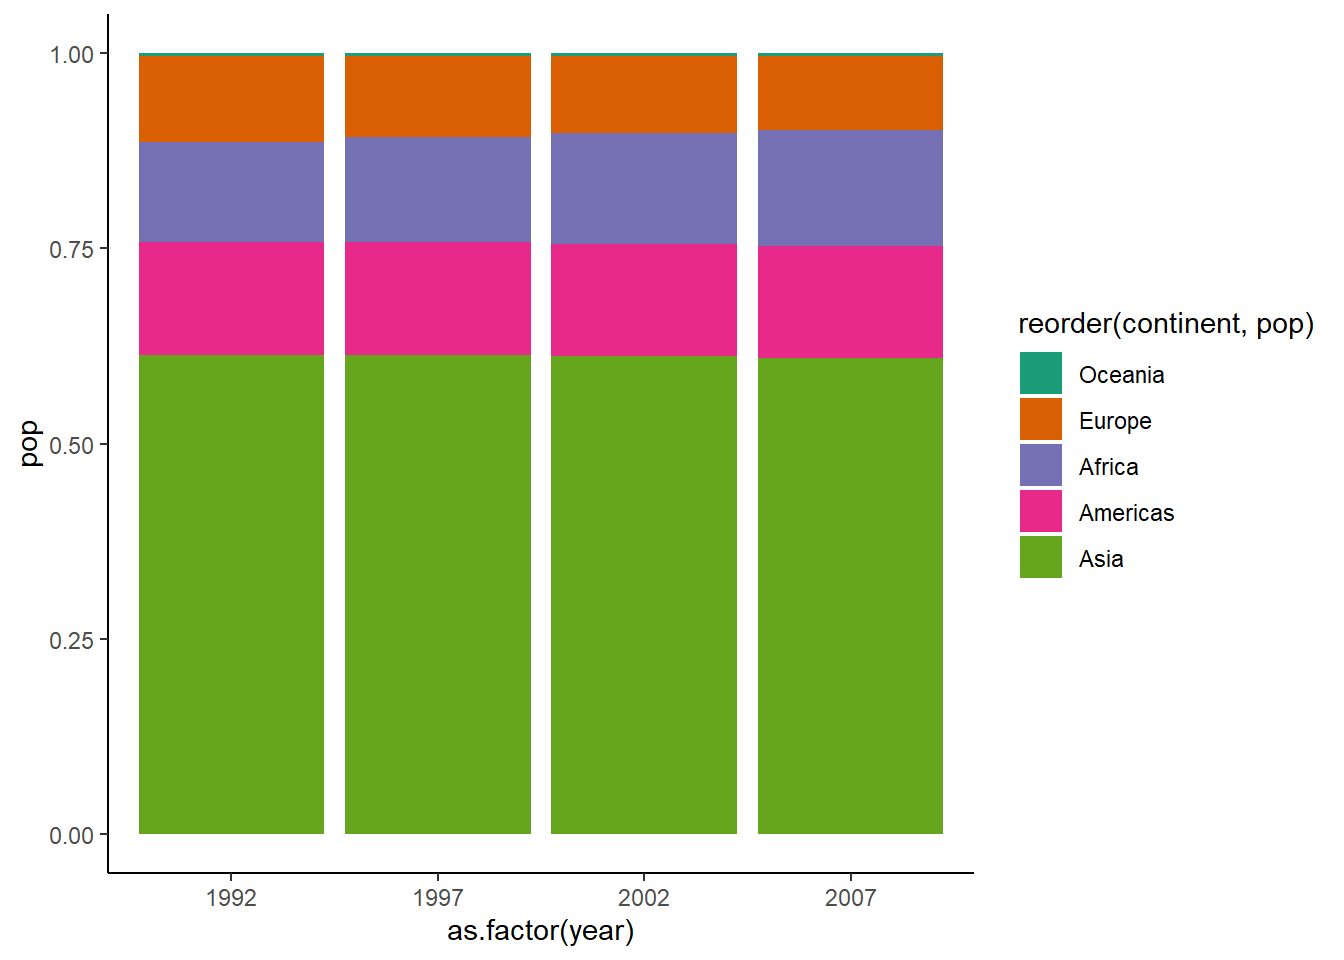
\includegraphics{03-datamanipulation_files/figure-latex/unnamed-chunk-52-1.pdf}

\begin{Shaded}
\begin{Highlighting}[]

\CommentTok{\# density plot}
\FunctionTok{plot}\NormalTok{(}\FunctionTok{density}\NormalTok{(gapminder\_xlsx\_2007}\SpecialCharTok{$}\NormalTok{gdpPercap))}
\end{Highlighting}
\end{Shaded}

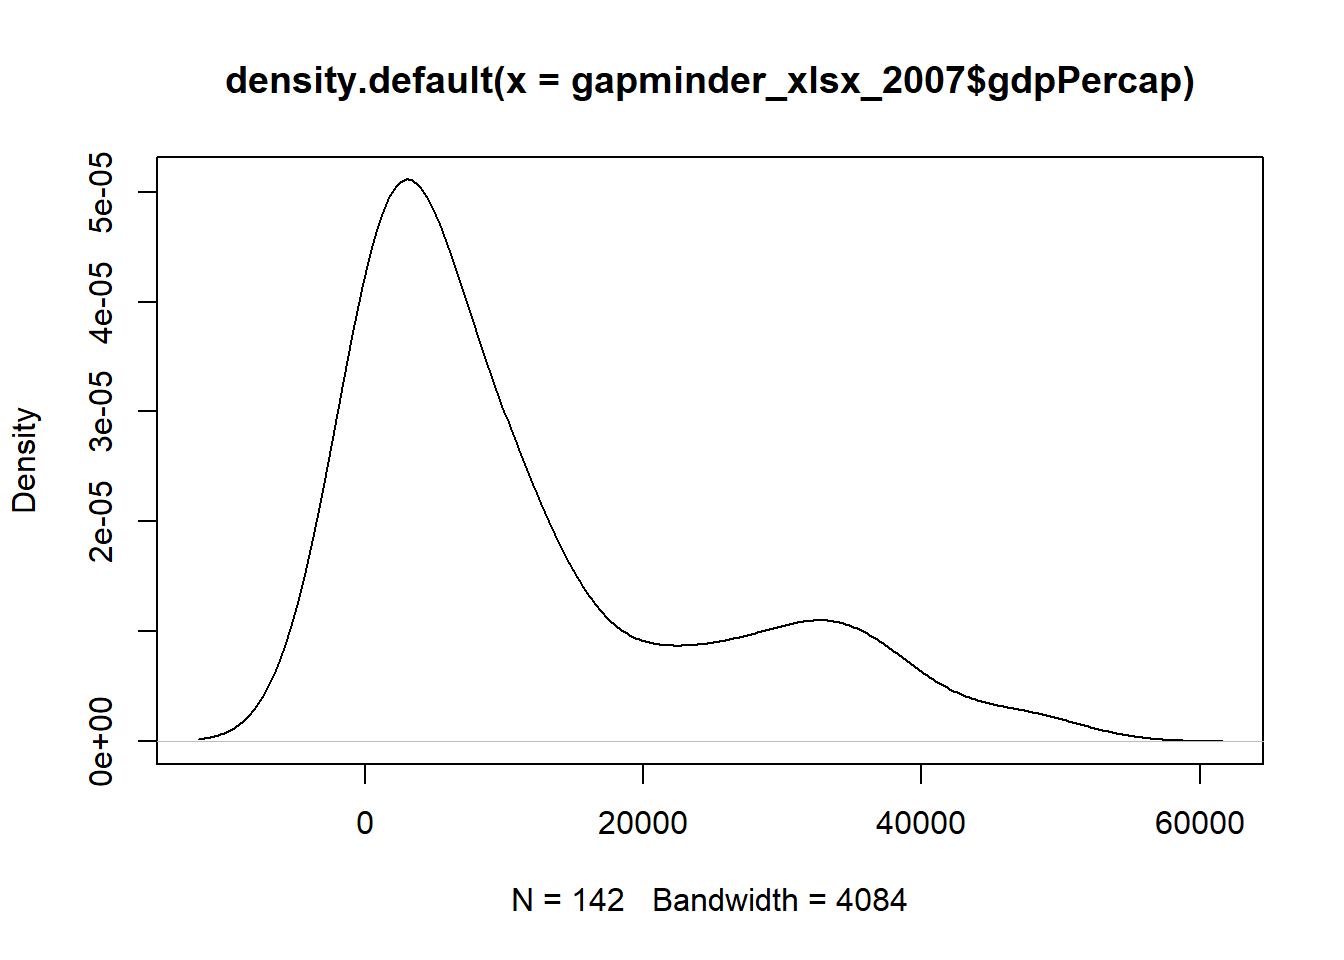
\includegraphics{03-datamanipulation_files/figure-latex/unnamed-chunk-52-2.pdf}

\begin{Shaded}
\begin{Highlighting}[]

\CommentTok{\# boxplot of population}
\FunctionTok{boxplot}\NormalTok{(gapminder\_xlsx\_2007}\SpecialCharTok{$}\NormalTok{gdpPercap)}
\end{Highlighting}
\end{Shaded}

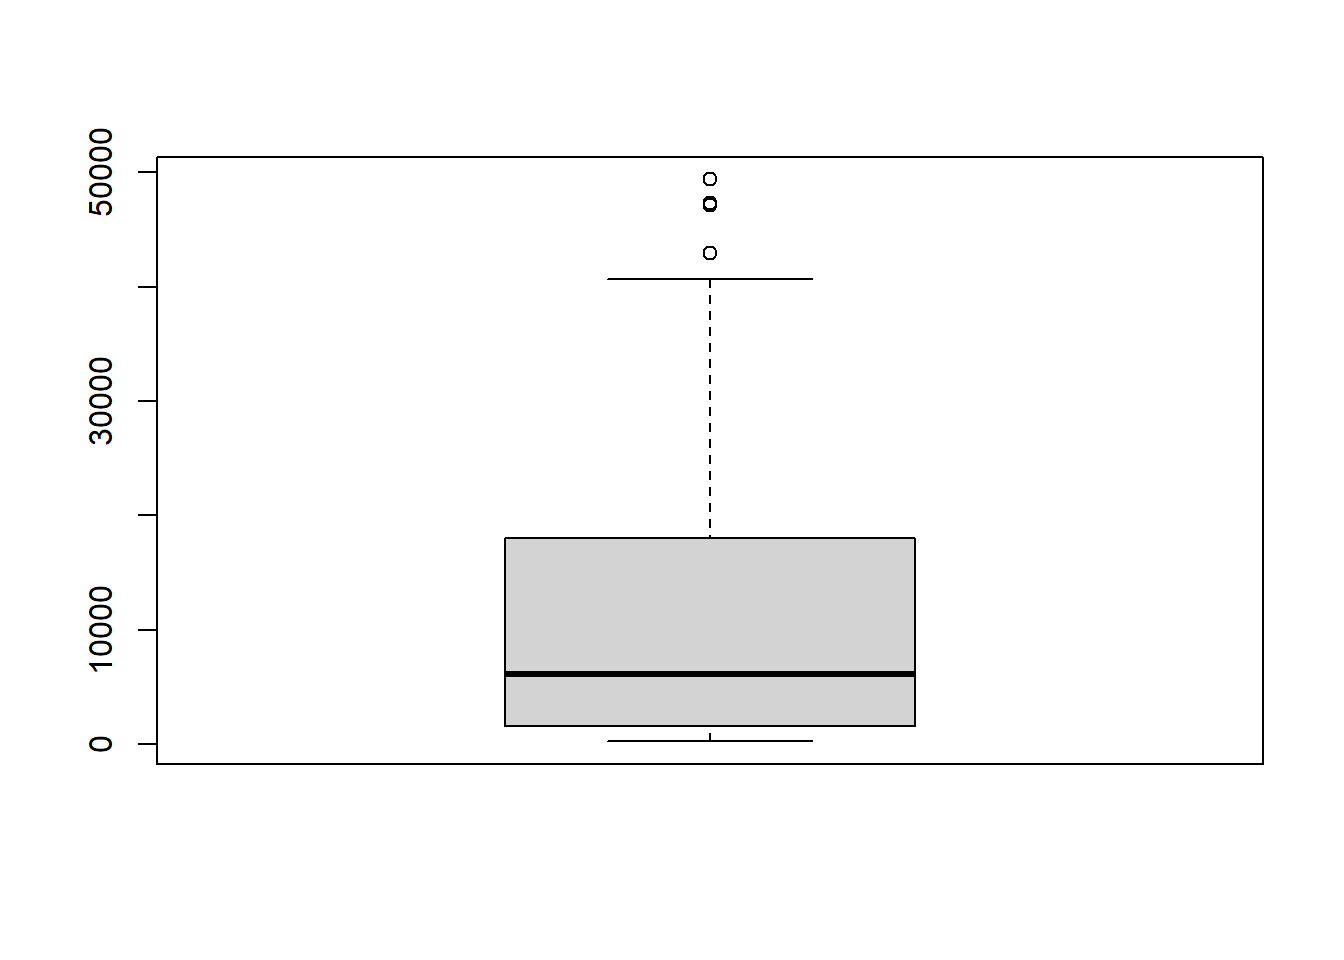
\includegraphics{03-datamanipulation_files/figure-latex/unnamed-chunk-52-3.pdf}

Of the above data visualizations, the boxplot is the most relevant as it shows both the spread of data and outliers. The boxplot reveals the following:

\begin{itemize}
\tightlist
\item
  minimum value,
\item
  first quantile (Q1),
\item
  median (second quantile),
\item
  third quantile (Q3),
\item
  maximum value excluding outliers and
\item
  outliers.
\end{itemize}

The difference between Q3 and Q1 is known as the Interquartile Range (IQR). The outliers within the box plot are calculated as any value that falls beyond 1.5 * IQR.

The function \texttt{boxplot.stats()} computes the data that is used to draw the box plot. Using this function, we can get our outliers.

\begin{Shaded}
\begin{Highlighting}[]
\FunctionTok{boxplot.stats}\NormalTok{(gapminder\_xlsx\_2007}\SpecialCharTok{$}\NormalTok{gdpPercap)}
\CommentTok{\#\textgreater{} $stats}
\CommentTok{\#\textgreater{} [1]   277.5519  1598.4351  6124.3711 18008.9444 40675.9964}
\CommentTok{\#\textgreater{} }
\CommentTok{\#\textgreater{} $n}
\CommentTok{\#\textgreater{} [1] 142}
\CommentTok{\#\textgreater{} }
\CommentTok{\#\textgreater{} $conf}
\CommentTok{\#\textgreater{} [1] 3948.491 8300.251}
\CommentTok{\#\textgreater{} }
\CommentTok{\#\textgreater{} $out}
\CommentTok{\#\textgreater{} [1] 47306.99 49357.19 47143.18 42951.65}
\end{Highlighting}
\end{Shaded}

The first element returned is the summary statistic as was calculated with \texttt{summary()}.

\begin{Shaded}
\begin{Highlighting}[]
\FunctionTok{boxplot.stats}\NormalTok{(gapminder\_xlsx\_2007}\SpecialCharTok{$}\NormalTok{gdpPercap)}\SpecialCharTok{$}\NormalTok{stats}
\CommentTok{\#\textgreater{} [1]   277.5519  1598.4351  6124.3711 18008.9444 40675.9964}
\FunctionTok{summary}\NormalTok{(gapminder\_xlsx\_2007}\SpecialCharTok{$}\NormalTok{gdpPercap)}
\CommentTok{\#\textgreater{}    Min. 1st Qu.  Median    Mean 3rd Qu.    Max. }
\CommentTok{\#\textgreater{}   277.6  1624.8  6124.4 11680.1 18008.8 49357.2}
\end{Highlighting}
\end{Shaded}

The last element returned are the outliers.

\begin{Shaded}
\begin{Highlighting}[]
\FunctionTok{boxplot.stats}\NormalTok{(gapminder\_xlsx\_2007}\SpecialCharTok{$}\NormalTok{gdpPercap)}\SpecialCharTok{$}\NormalTok{out}
\CommentTok{\#\textgreater{} [1] 47306.99 49357.19 47143.18 42951.65}
\end{Highlighting}
\end{Shaded}

Recall outliers are calculated as 1.5 * IQR, this can be changed using the argument coef. By default, it is set to 1.5 but can be changed as need be.

\begin{Shaded}
\begin{Highlighting}[]
\CommentTok{\# changing coef}
\FunctionTok{boxplot.stats}\NormalTok{(gapminder\_xlsx\_2007}\SpecialCharTok{$}\NormalTok{gdpPercap, }\AttributeTok{coef =} \FloatTok{0.8}\NormalTok{)}\SpecialCharTok{$}\NormalTok{out}
\CommentTok{\#\textgreater{}  [1] 34435.37 36126.49 33692.61 36319.24 35278.42 33207.08}
\CommentTok{\#\textgreater{}  [7] 32170.37 39724.98 36180.79 40676.00 31656.07 47306.99}
\CommentTok{\#\textgreater{} [13] 36797.93 49357.19 47143.18 33859.75 37506.42 33203.26}
\CommentTok{\#\textgreater{} [19] 42951.65}
\FunctionTok{boxplot.stats}\NormalTok{(gapminder\_xlsx\_2007}\SpecialCharTok{$}\NormalTok{gdpPercap, }\AttributeTok{coef =} \DecValTok{1}\NormalTok{)}\SpecialCharTok{$}\NormalTok{out}
\CommentTok{\#\textgreater{}  [1] 34435.37 36126.49 36319.24 35278.42 39724.98 36180.79}
\CommentTok{\#\textgreater{}  [7] 40676.00 47306.99 36797.93 49357.19 47143.18 37506.42}
\CommentTok{\#\textgreater{} [13] 42951.65}
\FunctionTok{boxplot.stats}\NormalTok{(gapminder\_xlsx\_2007}\SpecialCharTok{$}\NormalTok{gdpPercap, }\AttributeTok{coef =} \FloatTok{1.2}\NormalTok{)}\SpecialCharTok{$}\NormalTok{out}
\CommentTok{\#\textgreater{} [1] 39724.98 40676.00 47306.99 49357.19 47143.18 42951.65}

\CommentTok{\# selecting outliers}
\NormalTok{gapminder\_xlsx\_2007[gapminder\_xlsx\_2007}\SpecialCharTok{$}\NormalTok{gdpPercap }\SpecialCharTok{\textgreater{}=} \FunctionTok{min}\NormalTok{(}\FunctionTok{boxplot.stats}\NormalTok{(gapminder\_xlsx\_2007}\SpecialCharTok{$}\NormalTok{gdpPercap)}\SpecialCharTok{$}\NormalTok{out),]}
\CommentTok{\#\textgreater{}            country continent year lifeExp       pop}
\CommentTok{\#\textgreater{} 864         Kuwait      Asia 2007  77.588   2505559}
\CommentTok{\#\textgreater{} 1152        Norway    Europe 2007  80.196   4627926}
\CommentTok{\#\textgreater{} 1368     Singapore      Asia 2007  79.972   4553009}
\CommentTok{\#\textgreater{} 1620 United States  Americas 2007  78.242 301139947}
\CommentTok{\#\textgreater{}      gdpPercap      country\_hun continent\_hun}
\CommentTok{\#\textgreater{} 864   47306.99           Kuvait         Ázsia}
\CommentTok{\#\textgreater{} 1152  49357.19         Norvégia        Európa}
\CommentTok{\#\textgreater{} 1368  47143.18        Szingapúr         Ázsia}
\CommentTok{\#\textgreater{} 1620  42951.65 Egyesült Államok       Amerika}
\end{Highlighting}
\end{Shaded}

\hypertarget{dealing-with-duplicate-values}{%
\section{Dealing with duplicate values}\label{dealing-with-duplicate-values}}

\hypertarget{determining-duplicate-values}{%
\subsection{Determining duplicate values}\label{determining-duplicate-values}}

The function \texttt{duplicated()} determines which elements are duplicates in a vector or data frame while the function \texttt{anyDuplicated()} returns the index position of the first duplicate.

\begin{Shaded}
\begin{Highlighting}[]
\CommentTok{\# checking for duplicates}
\FunctionTok{duplicated}\NormalTok{(}\DecValTok{1}\SpecialCharTok{:}\DecValTok{10}\NormalTok{)}
\CommentTok{\#\textgreater{}  [1] FALSE FALSE FALSE FALSE FALSE FALSE FALSE FALSE FALSE}
\CommentTok{\#\textgreater{} [10] FALSE}

\FunctionTok{duplicated}\NormalTok{(}\FunctionTok{c}\NormalTok{(}\DecValTok{2}\NormalTok{, }\DecValTok{1}\NormalTok{, }\DecValTok{3}\NormalTok{, }\DecValTok{6}\NormalTok{, }\DecValTok{2}\NormalTok{, }\DecValTok{4}\NormalTok{, }\DecValTok{7}\NormalTok{, }\DecValTok{0}\NormalTok{, }\DecValTok{3}\NormalTok{, }\DecValTok{3}\NormalTok{, }\DecValTok{2}\NormalTok{, }\DecValTok{2}\NormalTok{, }\DecValTok{8}\NormalTok{, }\DecValTok{4}\NormalTok{, }\DecValTok{0}\NormalTok{))}
\CommentTok{\#\textgreater{}  [1] FALSE FALSE FALSE FALSE  TRUE FALSE FALSE FALSE  TRUE}
\CommentTok{\#\textgreater{} [10]  TRUE  TRUE  TRUE FALSE  TRUE  TRUE}

\CommentTok{\# get duplicate values}
\NormalTok{vt }\OtherTok{\textless{}{-}} \FunctionTok{c}\NormalTok{(}\DecValTok{2}\NormalTok{, }\DecValTok{1}\NormalTok{, }\DecValTok{3}\NormalTok{, }\DecValTok{6}\NormalTok{, }\DecValTok{2}\NormalTok{, }\DecValTok{4}\NormalTok{, }\DecValTok{7}\NormalTok{, }\DecValTok{0}\NormalTok{, }\DecValTok{3}\NormalTok{, }\DecValTok{3}\NormalTok{, }\DecValTok{2}\NormalTok{, }\DecValTok{2}\NormalTok{, }\DecValTok{8}\NormalTok{, }\DecValTok{4}\NormalTok{, }\DecValTok{0}\NormalTok{)}
\NormalTok{vt[}\FunctionTok{duplicated}\NormalTok{(}\FunctionTok{c}\NormalTok{(}\DecValTok{2}\NormalTok{, }\DecValTok{1}\NormalTok{, }\DecValTok{3}\NormalTok{, }\DecValTok{6}\NormalTok{, }\DecValTok{2}\NormalTok{, }\DecValTok{4}\NormalTok{, }\DecValTok{7}\NormalTok{, }\DecValTok{0}\NormalTok{, }\DecValTok{3}\NormalTok{, }\DecValTok{3}\NormalTok{, }\DecValTok{2}\NormalTok{, }\DecValTok{2}\NormalTok{, }\DecValTok{8}\NormalTok{, }\DecValTok{4}\NormalTok{, }\DecValTok{0}\NormalTok{))]}
\CommentTok{\#\textgreater{} [1] 2 3 3 2 2 4 0}

\CommentTok{\# checking if an object contains any duplicates}
\FunctionTok{any}\NormalTok{(}\FunctionTok{duplicated}\NormalTok{(}\DecValTok{1}\SpecialCharTok{:}\DecValTok{10}\NormalTok{))}
\CommentTok{\#\textgreater{} [1] FALSE}

\FunctionTok{any}\NormalTok{(}\FunctionTok{duplicated}\NormalTok{(}\FunctionTok{c}\NormalTok{(}\DecValTok{2}\NormalTok{, }\DecValTok{1}\NormalTok{, }\DecValTok{3}\NormalTok{, }\DecValTok{6}\NormalTok{, }\DecValTok{2}\NormalTok{, }\DecValTok{4}\NormalTok{, }\DecValTok{7}\NormalTok{, }\DecValTok{0}\NormalTok{, }\DecValTok{3}\NormalTok{, }\DecValTok{3}\NormalTok{, }\DecValTok{2}\NormalTok{, }\DecValTok{2}\NormalTok{, }\DecValTok{8}\NormalTok{, }\DecValTok{4}\NormalTok{, }\DecValTok{0}\NormalTok{)))}
\CommentTok{\#\textgreater{} [1] TRUE}

\CommentTok{\# get the first duplicate position}
\FunctionTok{anyDuplicated}\NormalTok{(}\DecValTok{1}\SpecialCharTok{:}\DecValTok{10}\NormalTok{)}
\CommentTok{\#\textgreater{} [1] 0}

\FunctionTok{anyDuplicated}\NormalTok{(}\FunctionTok{c}\NormalTok{(}\DecValTok{2}\NormalTok{, }\DecValTok{1}\NormalTok{, }\DecValTok{3}\NormalTok{, }\DecValTok{6}\NormalTok{, }\DecValTok{2}\NormalTok{, }\DecValTok{4}\NormalTok{, }\DecValTok{7}\NormalTok{, }\DecValTok{0}\NormalTok{, }\DecValTok{3}\NormalTok{, }\DecValTok{3}\NormalTok{, }\DecValTok{2}\NormalTok{, }\DecValTok{2}\NormalTok{, }\DecValTok{8}\NormalTok{, }\DecValTok{4}\NormalTok{, }\DecValTok{0}\NormalTok{))}
\CommentTok{\#\textgreater{} [1] 5}
\end{Highlighting}
\end{Shaded}

The function \texttt{duplicated()} and \texttt{anyDuplicated()} also work on data frames. The former drops unique rows while keeping duplicate rows.

\begin{Shaded}
\begin{Highlighting}[]
\NormalTok{movies\_2006 }\OtherTok{\textless{}{-}}\NormalTok{ mov[mov}\SpecialCharTok{$}\NormalTok{Year }\SpecialCharTok{==} \DecValTok{2006}\NormalTok{, }\FunctionTok{c}\NormalTok{(}\DecValTok{7}\NormalTok{,}\DecValTok{12}\NormalTok{)]}
\NormalTok{movies\_2006 }\OtherTok{\textless{}{-}}\NormalTok{ movies\_2006[}\FunctionTok{order}\NormalTok{(movies\_2006}\SpecialCharTok{$}\NormalTok{Year, movies\_2006}\SpecialCharTok{$}\NormalTok{Metascore),]}
\FunctionTok{head}\NormalTok{(movies\_2006)}
\CommentTok{\#\textgreater{}     Year Metascore}
\CommentTok{\#\textgreater{} 774 2006        36}
\CommentTok{\#\textgreater{} 309 2006        45}
\CommentTok{\#\textgreater{} 551 2006        45}
\CommentTok{\#\textgreater{} 594 2006        45}
\CommentTok{\#\textgreater{} 734 2006        46}
\CommentTok{\#\textgreater{} 531 2006        47}

\CommentTok{\# checking for any duplicates}
\FunctionTok{any}\NormalTok{(}\FunctionTok{duplicated}\NormalTok{(movies\_2006))}
\CommentTok{\#\textgreater{} [1] TRUE}

\FunctionTok{anyDuplicated}\NormalTok{(movies\_2006)}
\CommentTok{\#\textgreater{} [1] 3}

\CommentTok{\# checking for duplicates}
\FunctionTok{duplicated}\NormalTok{(movies\_2006)}
\CommentTok{\#\textgreater{}  [1] FALSE FALSE  TRUE  TRUE FALSE FALSE FALSE FALSE FALSE}
\CommentTok{\#\textgreater{} [10]  TRUE FALSE  TRUE FALSE FALSE  TRUE FALSE FALSE FALSE}
\CommentTok{\#\textgreater{} [19]  TRUE  TRUE FALSE FALSE  TRUE  TRUE  TRUE FALSE  TRUE}
\CommentTok{\#\textgreater{} [28] FALSE  TRUE FALSE FALSE FALSE FALSE  TRUE FALSE  TRUE}
\CommentTok{\#\textgreater{} [37] FALSE FALSE  TRUE FALSE FALSE FALSE  TRUE  TRUE}

\CommentTok{\# returning duplicates}
\NormalTok{movies\_2006\_dup }\OtherTok{\textless{}{-}}\NormalTok{ movies\_2006 [}\FunctionTok{duplicated}\NormalTok{(movies\_2006), ]}
\FunctionTok{head}\NormalTok{(movies\_2006\_dup)}
\CommentTok{\#\textgreater{}     Year Metascore}
\CommentTok{\#\textgreater{} 551 2006        45}
\CommentTok{\#\textgreater{} 594 2006        45}
\CommentTok{\#\textgreater{} 859 2006        52}
\CommentTok{\#\textgreater{} 960 2006        53}
\CommentTok{\#\textgreater{} 902 2006        58}
\CommentTok{\#\textgreater{} 670 2006        64}
\end{Highlighting}
\end{Shaded}

\hypertarget{get-unique-values}{%
\subsection{Get unique values}\label{get-unique-values}}

The function \texttt{unique()} extracts unique values from a vector or data frame.

\begin{Shaded}
\begin{Highlighting}[]
\CommentTok{\# return unique values}
\FunctionTok{unique}\NormalTok{(}\DecValTok{1}\SpecialCharTok{:}\DecValTok{10}\NormalTok{)}
\CommentTok{\#\textgreater{}  [1]  1  2  3  4  5  6  7  8  9 10}

\FunctionTok{unique}\NormalTok{(}\FunctionTok{c}\NormalTok{(}\DecValTok{2}\NormalTok{, }\DecValTok{1}\NormalTok{, }\DecValTok{3}\NormalTok{, }\DecValTok{6}\NormalTok{, }\DecValTok{2}\NormalTok{, }\DecValTok{4}\NormalTok{, }\DecValTok{7}\NormalTok{, }\DecValTok{0}\NormalTok{, }\DecValTok{3}\NormalTok{, }\DecValTok{3}\NormalTok{, }\DecValTok{2}\NormalTok{, }\DecValTok{2}\NormalTok{, }\DecValTok{8}\NormalTok{, }\DecValTok{4}\NormalTok{, }\DecValTok{0}\NormalTok{))}
\CommentTok{\#\textgreater{} [1] 2 1 3 6 4 7 0 8}

\CommentTok{\# return unique values using duplicated()}
\NormalTok{vt[}\SpecialCharTok{!}\FunctionTok{duplicated}\NormalTok{(}\FunctionTok{c}\NormalTok{(}\DecValTok{2}\NormalTok{, }\DecValTok{1}\NormalTok{, }\DecValTok{3}\NormalTok{, }\DecValTok{6}\NormalTok{, }\DecValTok{2}\NormalTok{, }\DecValTok{4}\NormalTok{, }\DecValTok{7}\NormalTok{, }\DecValTok{0}\NormalTok{, }\DecValTok{3}\NormalTok{, }\DecValTok{3}\NormalTok{, }\DecValTok{2}\NormalTok{, }\DecValTok{2}\NormalTok{, }\DecValTok{8}\NormalTok{, }\DecValTok{4}\NormalTok{, }\DecValTok{0}\NormalTok{))]}
\CommentTok{\#\textgreater{} [1] 2 1 3 6 4 7 0 8}

\CommentTok{\# returning unique rows}
\NormalTok{movies\_2006\_uni }\OtherTok{\textless{}{-}} \FunctionTok{unique}\NormalTok{(movies\_2006)}
\FunctionTok{head}\NormalTok{(movies\_2006\_uni)}
\CommentTok{\#\textgreater{}     Year Metascore}
\CommentTok{\#\textgreater{} 774 2006        36}
\CommentTok{\#\textgreater{} 309 2006        45}
\CommentTok{\#\textgreater{} 734 2006        46}
\CommentTok{\#\textgreater{} 531 2006        47}
\CommentTok{\#\textgreater{} 321 2006        48}
\CommentTok{\#\textgreater{} 775 2006        51}

\CommentTok{\# returning unique rows using duplicated()}
\NormalTok{movies\_2006\_uni }\OtherTok{\textless{}{-}} \FunctionTok{subset}\NormalTok{(movies\_2006, }\SpecialCharTok{!}\FunctionTok{duplicated}\NormalTok{(movies\_2006))}
\FunctionTok{head}\NormalTok{(movies\_2006\_uni)}
\CommentTok{\#\textgreater{}     Year Metascore}
\CommentTok{\#\textgreater{} 774 2006        36}
\CommentTok{\#\textgreater{} 309 2006        45}
\CommentTok{\#\textgreater{} 734 2006        46}
\CommentTok{\#\textgreater{} 531 2006        47}
\CommentTok{\#\textgreater{} 321 2006        48}
\CommentTok{\#\textgreater{} 775 2006        51}
\end{Highlighting}
\end{Shaded}

\hypertarget{br-factor}{%
\section{Factors in Base R}\label{br-factor}}

\hypertarget{what-are-factors}{%
\subsection{What are factors?}\label{what-are-factors}}

Factors are variables in R which take on a limited number of different values which are usually known as categorical values e.g.~male and female or months of the year. They can contain either strings or integers but are stored internally as a vector of integers with each integer corresponding to one category.
Factors can either be ordered or unordered e.g.~low, medium, high for ordered and male or female for unordered.

\hypertarget{creating-a-factor}{%
\subsection{Creating a factor}\label{creating-a-factor}}

While the function \texttt{factor()} is used to create a factor, the function \texttt{is.factor()} is used to check for factor.

\begin{Shaded}
\begin{Highlighting}[]
\CommentTok{\# creating a factor}
\NormalTok{(fac }\OtherTok{\textless{}{-}} \FunctionTok{factor}\NormalTok{(}\FunctionTok{c}\NormalTok{(}\StringTok{\textquotesingle{}female\textquotesingle{}}\NormalTok{, }\StringTok{\textquotesingle{}male\textquotesingle{}}\NormalTok{, }\StringTok{\textquotesingle{}male\textquotesingle{}}\NormalTok{, }\StringTok{\textquotesingle{}female\textquotesingle{}}\NormalTok{, }\StringTok{\textquotesingle{}male\textquotesingle{}}\NormalTok{, }\StringTok{\textquotesingle{}male\textquotesingle{}}\NormalTok{, }\StringTok{\textquotesingle{}male\textquotesingle{}}\NormalTok{, }\StringTok{\textquotesingle{}female\textquotesingle{}}\NormalTok{)))}
\CommentTok{\#\textgreater{} [1] female male   male   female male   male   male   female}
\CommentTok{\#\textgreater{} Levels: female male}

\CommentTok{\# looking at type and class}
\FunctionTok{typeof}\NormalTok{(fac)}
\CommentTok{\#\textgreater{} [1] "integer"}
\FunctionTok{class}\NormalTok{(fac)}
\CommentTok{\#\textgreater{} [1] "factor"}

\CommentTok{\# checking if the object is a factor}
\FunctionTok{is.factor}\NormalTok{(fac)}
\CommentTok{\#\textgreater{} [1] TRUE}
\end{Highlighting}
\end{Shaded}

\hypertarget{factor-attributes-and-structure}{%
\subsection{Factor attributes and structure}\label{factor-attributes-and-structure}}

A factor has as attribute levels which represent the categories of the factor.
The function \texttt{levels()} is used to get and set levels while \texttt{nlevels()} returns the number of categories.

\begin{Shaded}
\begin{Highlighting}[]
\CommentTok{\# get levels}
\FunctionTok{levels}\NormalTok{(fac)}
\CommentTok{\#\textgreater{} [1] "female" "male"}

\CommentTok{\# set levels}
\NormalTok{(}\FunctionTok{levels}\NormalTok{(fac) }\OtherTok{\textless{}{-}} \FunctionTok{c}\NormalTok{(}\StringTok{\textquotesingle{}f\textquotesingle{}}\NormalTok{, }\StringTok{\textquotesingle{}m\textquotesingle{}}\NormalTok{))}
\CommentTok{\#\textgreater{} [1] "f" "m"}

\CommentTok{\# resetting levels}
\NormalTok{(}\FunctionTok{levels}\NormalTok{(fac) }\OtherTok{\textless{}{-}} \FunctionTok{c}\NormalTok{(}\StringTok{\textquotesingle{}female\textquotesingle{}}\NormalTok{, }\StringTok{\textquotesingle{}male\textquotesingle{}}\NormalTok{))}
\CommentTok{\#\textgreater{} [1] "female" "male"}

\CommentTok{\# number of categories}
\FunctionTok{nlevels}\NormalTok{(fac)}
\CommentTok{\#\textgreater{} [1] 2}

\CommentTok{\# structure of the factor}
\FunctionTok{str}\NormalTok{(fac)}
\CommentTok{\#\textgreater{}  Factor w/ 2 levels "female","male": 1 2 2 1 2 2 2 1}

\FunctionTok{attributes}\NormalTok{(fac)}
\CommentTok{\#\textgreater{} $levels}
\CommentTok{\#\textgreater{} [1] "female" "male"  }
\CommentTok{\#\textgreater{} }
\CommentTok{\#\textgreater{} $class}
\CommentTok{\#\textgreater{} [1] "factor"}

\CommentTok{\# count of elements by category}
\FunctionTok{table}\NormalTok{(fac)}
\CommentTok{\#\textgreater{} fac}
\CommentTok{\#\textgreater{} female   male }
\CommentTok{\#\textgreater{}      3      5}

\CommentTok{\# internally factors are stored as integers}
\FunctionTok{unclass}\NormalTok{(fac)}
\CommentTok{\#\textgreater{} [1] 1 2 2 1 2 2 2 1}
\CommentTok{\#\textgreater{} attr(,"levels")}
\CommentTok{\#\textgreater{} [1] "female" "male"}
\end{Highlighting}
\end{Shaded}

\hypertarget{rearranging-levels}{%
\subsection{Rearranging levels}\label{rearranging-levels}}

The argument levels is used to rearrange the levels of a factor.

\begin{Shaded}
\begin{Highlighting}[]
\NormalTok{lev }\OtherTok{\textless{}{-}} \FunctionTok{c}\NormalTok{(}\StringTok{\textquotesingle{}male\textquotesingle{}}\NormalTok{, }\StringTok{\textquotesingle{}female\textquotesingle{}}\NormalTok{)}
\NormalTok{(fac1 }\OtherTok{\textless{}{-}} \FunctionTok{factor}\NormalTok{(}\FunctionTok{c}\NormalTok{(}\StringTok{\textquotesingle{}female\textquotesingle{}}\NormalTok{, }\StringTok{\textquotesingle{}male\textquotesingle{}}\NormalTok{, }\StringTok{\textquotesingle{}male\textquotesingle{}}\NormalTok{, }\StringTok{\textquotesingle{}female\textquotesingle{}}\NormalTok{, }\StringTok{\textquotesingle{}male\textquotesingle{}}\NormalTok{, }\StringTok{\textquotesingle{}male\textquotesingle{}}\NormalTok{, }\StringTok{\textquotesingle{}male\textquotesingle{}}\NormalTok{, }\StringTok{\textquotesingle{}female\textquotesingle{}}\NormalTok{), }
               \AttributeTok{levels =}\NormalTok{ lev))}
\CommentTok{\#\textgreater{} [1] female male   male   female male   male   male   female}
\CommentTok{\#\textgreater{} Levels: male female}

\CommentTok{\# comparing fac and fac1}
\FunctionTok{attributes}\NormalTok{(fac)}
\CommentTok{\#\textgreater{} $levels}
\CommentTok{\#\textgreater{} [1] "female" "male"  }
\CommentTok{\#\textgreater{} }
\CommentTok{\#\textgreater{} $class}
\CommentTok{\#\textgreater{} [1] "factor"}
\FunctionTok{attributes}\NormalTok{(fac1)}
\CommentTok{\#\textgreater{} $levels}
\CommentTok{\#\textgreater{} [1] "male"   "female"}
\CommentTok{\#\textgreater{} }
\CommentTok{\#\textgreater{} $class}
\CommentTok{\#\textgreater{} [1] "factor"}

\FunctionTok{table}\NormalTok{(fac) }
\CommentTok{\#\textgreater{} fac}
\CommentTok{\#\textgreater{} female   male }
\CommentTok{\#\textgreater{}      3      5}
\FunctionTok{table}\NormalTok{(fac1)}
\CommentTok{\#\textgreater{} fac1}
\CommentTok{\#\textgreater{}   male female }
\CommentTok{\#\textgreater{}      5      3}
\end{Highlighting}
\end{Shaded}

\hypertarget{dropping-levels}{%
\subsection{Dropping levels}\label{dropping-levels}}

The function \texttt{droplevels()} is used to drop unused levels from a factor.

\begin{Shaded}
\begin{Highlighting}[]
\NormalTok{(fac1 }\OtherTok{\textless{}{-}} \FunctionTok{factor}\NormalTok{(}\FunctionTok{c}\NormalTok{(}\StringTok{\textquotesingle{}female\textquotesingle{}}\NormalTok{, }\StringTok{\textquotesingle{}male\textquotesingle{}}\NormalTok{, }\StringTok{\textquotesingle{}male\textquotesingle{}}\NormalTok{, }\StringTok{\textquotesingle{}female\textquotesingle{}}\NormalTok{, }\StringTok{\textquotesingle{}male\textquotesingle{}}\NormalTok{, }\StringTok{\textquotesingle{}male\textquotesingle{}}\NormalTok{, }\StringTok{\textquotesingle{}male\textquotesingle{}}\NormalTok{, }\StringTok{\textquotesingle{}female\textquotesingle{}}\NormalTok{), }
               \AttributeTok{levels =} \FunctionTok{c}\NormalTok{(}\StringTok{\textquotesingle{}male\textquotesingle{}}\NormalTok{, }\StringTok{\textquotesingle{}female\textquotesingle{}}\NormalTok{, }\StringTok{\textquotesingle{}boy\textquotesingle{}}\NormalTok{, }\StringTok{\textquotesingle{}girl\textquotesingle{}}\NormalTok{)))}
\CommentTok{\#\textgreater{} [1] female male   male   female male   male   male   female}
\CommentTok{\#\textgreater{} Levels: male female boy girl}
\NormalTok{(fac1 }\OtherTok{\textless{}{-}} \FunctionTok{droplevels}\NormalTok{(fac1))}
\CommentTok{\#\textgreater{} [1] female male   male   female male   male   male   female}
\CommentTok{\#\textgreater{} Levels: male female}
\end{Highlighting}
\end{Shaded}

\hypertarget{changing-labels}{%
\subsection{Changing labels}\label{changing-labels}}

The argument label is used to change the labels of a factor.

\begin{Shaded}
\begin{Highlighting}[]
\CommentTok{\# changing from male to M and from female to F}
\NormalTok{(fac1 }\OtherTok{\textless{}{-}} \FunctionTok{factor}\NormalTok{(}\FunctionTok{c}\NormalTok{(}\StringTok{\textquotesingle{}female\textquotesingle{}}\NormalTok{, }\StringTok{\textquotesingle{}male\textquotesingle{}}\NormalTok{, }\StringTok{\textquotesingle{}male\textquotesingle{}}\NormalTok{, }\StringTok{\textquotesingle{}female\textquotesingle{}}\NormalTok{, }\StringTok{\textquotesingle{}male\textquotesingle{}}\NormalTok{, }\StringTok{\textquotesingle{}male\textquotesingle{}}\NormalTok{, }\StringTok{\textquotesingle{}male\textquotesingle{}}\NormalTok{, }\StringTok{\textquotesingle{}female\textquotesingle{}}\NormalTok{), }
               \AttributeTok{levels =} \FunctionTok{c}\NormalTok{(}\StringTok{\textquotesingle{}male\textquotesingle{}}\NormalTok{, }\StringTok{\textquotesingle{}female\textquotesingle{}}\NormalTok{), }
               \AttributeTok{label =} \FunctionTok{c}\NormalTok{(}\StringTok{\textquotesingle{}M\textquotesingle{}}\NormalTok{, }\StringTok{\textquotesingle{}F\textquotesingle{}}\NormalTok{)))}
\CommentTok{\#\textgreater{} [1] F M M F M M M F}
\CommentTok{\#\textgreater{} Levels: M F}
\end{Highlighting}
\end{Shaded}

\hypertarget{ordered-factors}{%
\subsection{Ordered factors}\label{ordered-factors}}

Ordered factors are factors whose orders matter for example with grading; A is greater than B and B greater than C, and so forth. The argument \texttt{order\ =\ TRUE} is used to create an ordered factor. Also, the function \texttt{ordered()} can be used to create an ordered factor while the function \texttt{is.ordered()} is used to check for ordered factor. With ordered factors, we can use the function \texttt{min()} and \texttt{max()} on them to determine the minimum and maximum values, respectively.

\begin{Shaded}
\begin{Highlighting}[]
\NormalTok{(fac2 }\OtherTok{\textless{}{-}} \FunctionTok{factor}\NormalTok{(}\FunctionTok{c}\NormalTok{(}\StringTok{\textquotesingle{}female\textquotesingle{}}\NormalTok{, }\StringTok{\textquotesingle{}male\textquotesingle{}}\NormalTok{, }\StringTok{\textquotesingle{}male\textquotesingle{}}\NormalTok{, }\StringTok{\textquotesingle{}female\textquotesingle{}}\NormalTok{, }\StringTok{\textquotesingle{}male\textquotesingle{}}\NormalTok{, }\StringTok{\textquotesingle{}male\textquotesingle{}}\NormalTok{, }\StringTok{\textquotesingle{}male\textquotesingle{}}\NormalTok{, }\StringTok{\textquotesingle{}female\textquotesingle{}}\NormalTok{), }
               \AttributeTok{levels =}\NormalTok{ lev, }
               \AttributeTok{ordered =}\NormalTok{ T))}
\CommentTok{\#\textgreater{} [1] female male   male   female male   male   male   female}
\CommentTok{\#\textgreater{} Levels: male \textless{} female}
\FunctionTok{attributes}\NormalTok{(fac)}
\CommentTok{\#\textgreater{} $levels}
\CommentTok{\#\textgreater{} [1] "female" "male"  }
\CommentTok{\#\textgreater{} }
\CommentTok{\#\textgreater{} $class}
\CommentTok{\#\textgreater{} [1] "factor"}
\FunctionTok{attributes}\NormalTok{(fac1)}
\CommentTok{\#\textgreater{} $levels}
\CommentTok{\#\textgreater{} [1] "M" "F"}
\CommentTok{\#\textgreater{} }
\CommentTok{\#\textgreater{} $class}
\CommentTok{\#\textgreater{} [1] "factor"}
\FunctionTok{attributes}\NormalTok{(fac2)}
\CommentTok{\#\textgreater{} $levels}
\CommentTok{\#\textgreater{} [1] "male"   "female"}
\CommentTok{\#\textgreater{} }
\CommentTok{\#\textgreater{} $class}
\CommentTok{\#\textgreater{} [1] "ordered" "factor"}

\CommentTok{\# getting minimum and maximum values}
\FunctionTok{min}\NormalTok{(fac2)}
\CommentTok{\#\textgreater{} [1] male}
\CommentTok{\#\textgreater{} Levels: male \textless{} female}
\FunctionTok{max}\NormalTok{(fac2)}
\CommentTok{\#\textgreater{} [1] female}
\CommentTok{\#\textgreater{} Levels: male \textless{} female}

\CommentTok{\# checking for ordered factor}
\FunctionTok{is.ordered}\NormalTok{(fac2)}
\CommentTok{\#\textgreater{} [1] TRUE}

\FunctionTok{ordered}\NormalTok{(}\FunctionTok{c}\NormalTok{(}\StringTok{\textquotesingle{}female\textquotesingle{}}\NormalTok{, }\StringTok{\textquotesingle{}male\textquotesingle{}}\NormalTok{, }\StringTok{\textquotesingle{}male\textquotesingle{}}\NormalTok{, }\StringTok{\textquotesingle{}female\textquotesingle{}}\NormalTok{, }\StringTok{\textquotesingle{}male\textquotesingle{}}\NormalTok{, }\StringTok{\textquotesingle{}male\textquotesingle{}}\NormalTok{, }\StringTok{\textquotesingle{}male\textquotesingle{}}\NormalTok{, }\StringTok{\textquotesingle{}female\textquotesingle{}}\NormalTok{))}
\CommentTok{\#\textgreater{} [1] female male   male   female male   male   male   female}
\CommentTok{\#\textgreater{} Levels: female \textless{} male}
\FunctionTok{ordered}\NormalTok{(}\FunctionTok{c}\NormalTok{(}\StringTok{\textquotesingle{}female\textquotesingle{}}\NormalTok{, }\StringTok{\textquotesingle{}male\textquotesingle{}}\NormalTok{, }\StringTok{\textquotesingle{}male\textquotesingle{}}\NormalTok{, }\StringTok{\textquotesingle{}female\textquotesingle{}}\NormalTok{, }\StringTok{\textquotesingle{}male\textquotesingle{}}\NormalTok{, }\StringTok{\textquotesingle{}male\textquotesingle{}}\NormalTok{, }\StringTok{\textquotesingle{}male\textquotesingle{}}\NormalTok{, }\StringTok{\textquotesingle{}female\textquotesingle{}}\NormalTok{), }
        \AttributeTok{levels =} \FunctionTok{c}\NormalTok{(}\StringTok{\textquotesingle{}male\textquotesingle{}}\NormalTok{, }\StringTok{\textquotesingle{}female\textquotesingle{}}\NormalTok{))}
\CommentTok{\#\textgreater{} [1] female male   male   female male   male   male   female}
\CommentTok{\#\textgreater{} Levels: male \textless{} female}
\end{Highlighting}
\end{Shaded}

The functions \texttt{max()} and \texttt{min()} do not work for \texttt{fac} and \texttt{fac1} because they are not ordered, hence have no minimum or maximum.

\hypertarget{converting-from-character-to-factor}{%
\subsection{Converting from character to factor}\label{converting-from-character-to-factor}}

The function \texttt{as.factor()} converts to a factor, if possible but is less flexible than \texttt{factor()}. It is used when we do not care about levels, label or order.

\begin{Shaded}
\begin{Highlighting}[]
\NormalTok{month.name}
\CommentTok{\#\textgreater{}  [1] "January"   "February"  "March"     "April"    }
\CommentTok{\#\textgreater{}  [5] "May"       "June"      "July"      "August"   }
\CommentTok{\#\textgreater{}  [9] "September" "October"   "November"  "December"}
\FunctionTok{class}\NormalTok{(month.name)}
\CommentTok{\#\textgreater{} [1] "character"}

\CommentTok{\# converting to factor}
\NormalTok{(month\_fac }\OtherTok{\textless{}{-}} \FunctionTok{as.factor}\NormalTok{(month.name))}
\CommentTok{\#\textgreater{}  [1] January   February  March     April     May      }
\CommentTok{\#\textgreater{}  [6] June      July      August    September October  }
\CommentTok{\#\textgreater{} [11] November  December }
\CommentTok{\#\textgreater{} 12 Levels: April August December February January ... September}
\end{Highlighting}
\end{Shaded}

\hypertarget{converting-from-factor-to-character}{%
\subsection{Converting from factor to character}\label{converting-from-factor-to-character}}

The function \texttt{as.character()} converts from factor to character.

\texttt{(month\_char\ \textless{}-\ as.character(month\_fac))}

\hypertarget{converting-from-numeric-to-factor}{%
\subsection{Converting from numeric to factor}\label{converting-from-numeric-to-factor}}

The function \texttt{cut()} is used to convert from numeric vector to factor. It bins numbers into ranges which can be treated as categories.

\begin{Shaded}
\begin{Highlighting}[]
\NormalTok{scores }\OtherTok{\textless{}{-}} \FunctionTok{c}\NormalTok{(}\DecValTok{15}\NormalTok{,}\DecValTok{65}\NormalTok{,}\DecValTok{68}\NormalTok{,}\DecValTok{46}\NormalTok{,}\DecValTok{15}\NormalTok{,}\DecValTok{61}\NormalTok{,}\DecValTok{32}\NormalTok{,}\DecValTok{13}\NormalTok{,}\DecValTok{15}\NormalTok{,}\DecValTok{46}\NormalTok{,}\DecValTok{13}\NormalTok{,}\DecValTok{21}\NormalTok{,}\DecValTok{89}\NormalTok{,}\DecValTok{89}\NormalTok{,}\DecValTok{44}\NormalTok{,}\DecValTok{51}\NormalTok{,}\DecValTok{32}\NormalTok{,}\DecValTok{16}\NormalTok{,}\DecValTok{18}\NormalTok{,}\DecValTok{95}\NormalTok{,}\DecValTok{46}\NormalTok{,}\DecValTok{16}\NormalTok{,}\DecValTok{65}\NormalTok{,}\DecValTok{46}\NormalTok{)}

\CommentTok{\# create factors from numeric}
\FunctionTok{cut}\NormalTok{(scores, }\AttributeTok{breaks =} \DecValTok{5}\NormalTok{)}
\CommentTok{\#\textgreater{}  [1] (12.9,29.4] (62.2,78.6] (62.2,78.6] (45.8,62.2]}
\CommentTok{\#\textgreater{}  [5] (12.9,29.4] (45.8,62.2] (29.4,45.8] (12.9,29.4]}
\CommentTok{\#\textgreater{}  [9] (12.9,29.4] (45.8,62.2] (12.9,29.4] (12.9,29.4]}
\CommentTok{\#\textgreater{} [13] (78.6,95.1] (78.6,95.1] (29.4,45.8] (45.8,62.2]}
\CommentTok{\#\textgreater{} [17] (29.4,45.8] (12.9,29.4] (12.9,29.4] (78.6,95.1]}
\CommentTok{\#\textgreater{} [21] (45.8,62.2] (12.9,29.4] (62.2,78.6] (45.8,62.2]}
\CommentTok{\#\textgreater{} 5 Levels: (12.9,29.4] (29.4,45.8] ... (78.6,95.1]}

\CommentTok{\# return categories}
\FunctionTok{levels}\NormalTok{(}\FunctionTok{cut}\NormalTok{(scores, }\AttributeTok{breaks =} \DecValTok{5}\NormalTok{))}
\CommentTok{\#\textgreater{} [1] "(12.9,29.4]" "(29.4,45.8]" "(45.8,62.2]" "(62.2,78.6]"}
\CommentTok{\#\textgreater{} [5] "(78.6,95.1]"}

\CommentTok{\# number of levels}
\FunctionTok{nlevels}\NormalTok{(}\FunctionTok{cut}\NormalTok{(scores, }\AttributeTok{breaks =} \DecValTok{5}\NormalTok{))}
\CommentTok{\#\textgreater{} [1] 5}

\CommentTok{\# check class}
\FunctionTok{class}\NormalTok{(}\FunctionTok{cut}\NormalTok{(scores, }\AttributeTok{breaks =} \DecValTok{5}\NormalTok{))}
\CommentTok{\#\textgreater{} [1] "factor"}

\CommentTok{\# controlling breaks}
\FunctionTok{cut}\NormalTok{(scores, }\AttributeTok{breaks =} \FunctionTok{c}\NormalTok{(}\DecValTok{0}\NormalTok{, }\DecValTok{40}\NormalTok{ , }\DecValTok{50}\NormalTok{, }\DecValTok{60}\NormalTok{, }\DecValTok{80}\NormalTok{, }\DecValTok{100}\NormalTok{))}
\CommentTok{\#\textgreater{}  [1] (0,40]   (60,80]  (60,80]  (40,50]  (0,40]   (60,80] }
\CommentTok{\#\textgreater{}  [7] (0,40]   (0,40]   (0,40]   (40,50]  (0,40]   (0,40]  }
\CommentTok{\#\textgreater{} [13] (80,100] (80,100] (40,50]  (50,60]  (0,40]   (0,40]  }
\CommentTok{\#\textgreater{} [19] (0,40]   (80,100] (40,50]  (0,40]   (60,80]  (40,50] }
\CommentTok{\#\textgreater{} Levels: (0,40] (40,50] (50,60] (60,80] (80,100]}

\CommentTok{\# adding labels}
\FunctionTok{cut}\NormalTok{(scores, }\AttributeTok{breaks =} \FunctionTok{c}\NormalTok{(}\DecValTok{0}\NormalTok{, }\DecValTok{40}\NormalTok{ , }\DecValTok{50}\NormalTok{, }\DecValTok{60}\NormalTok{, }\DecValTok{80}\NormalTok{, }\DecValTok{100}\NormalTok{), }\AttributeTok{labels =} \FunctionTok{c}\NormalTok{(}\StringTok{\textquotesingle{}F\textquotesingle{}}\NormalTok{, }\StringTok{\textquotesingle{}D\textquotesingle{}}\NormalTok{, }\StringTok{\textquotesingle{}C\textquotesingle{}}\NormalTok{, }\StringTok{\textquotesingle{}B\textquotesingle{}}\NormalTok{, }\StringTok{\textquotesingle{}A\textquotesingle{}}\NormalTok{))}
\CommentTok{\#\textgreater{}  [1] F B B D F B F F F D F F A A D C F F F A D F B D}
\CommentTok{\#\textgreater{} Levels: F D C B A}

\CommentTok{\# majority of the students failed}
\FunctionTok{table}\NormalTok{(}\FunctionTok{cut}\NormalTok{(scores, }\AttributeTok{breaks =} \FunctionTok{c}\NormalTok{(}\DecValTok{0}\NormalTok{, }\DecValTok{40}\NormalTok{ , }\DecValTok{50}\NormalTok{, }\DecValTok{60}\NormalTok{, }\DecValTok{80}\NormalTok{, }\DecValTok{100}\NormalTok{), }\AttributeTok{labels =} \FunctionTok{c}\NormalTok{(}\StringTok{\textquotesingle{}F\textquotesingle{}}\NormalTok{, }\StringTok{\textquotesingle{}D\textquotesingle{}}\NormalTok{, }\StringTok{\textquotesingle{}C\textquotesingle{}}\NormalTok{, }\StringTok{\textquotesingle{}B\textquotesingle{}}\NormalTok{, }\StringTok{\textquotesingle{}A\textquotesingle{}}\NormalTok{)))}
\CommentTok{\#\textgreater{} }
\CommentTok{\#\textgreater{}  F  D  C  B  A }
\CommentTok{\#\textgreater{} 11  5  1  4  3}
\end{Highlighting}
\end{Shaded}

\hypertarget{converting-from-factor-to-numeric}{%
\subsection{Converting from factor to numeric}\label{converting-from-factor-to-numeric}}

To convert from a factor to numeric, the function \texttt{as.numeric()} does not work. To use it, we first have to convert the factor to character using \texttt{as.character()} or \texttt{levels(fac){[}fac{]}}. Below we make use of both methods to achieve our objective.

\begin{Shaded}
\begin{Highlighting}[]
\NormalTok{num\_vec }\OtherTok{\textless{}{-}} \FunctionTok{c}\NormalTok{(}\DecValTok{15}\NormalTok{,}\DecValTok{65}\NormalTok{,}\DecValTok{68}\NormalTok{,}\DecValTok{46}\NormalTok{,}\DecValTok{15}\NormalTok{,}\DecValTok{61}\NormalTok{,}\DecValTok{32}\NormalTok{,}\DecValTok{13}\NormalTok{,}\DecValTok{15}\NormalTok{,}\DecValTok{46}\NormalTok{,}\DecValTok{13}\NormalTok{,}\DecValTok{21}\NormalTok{,}\DecValTok{89}\NormalTok{,}\DecValTok{89}\NormalTok{,}\DecValTok{44}\NormalTok{,}\DecValTok{51}\NormalTok{,}\DecValTok{32}\NormalTok{,}\DecValTok{16}\NormalTok{,}\DecValTok{18}\NormalTok{,}\DecValTok{95}\NormalTok{,}\DecValTok{46}\NormalTok{,}\DecValTok{16}\NormalTok{,}\DecValTok{65}\NormalTok{,}\DecValTok{46}\NormalTok{)}
\FunctionTok{mean}\NormalTok{(num\_vec)}
\CommentTok{\#\textgreater{} [1] 42.375}

\CommentTok{\#converting to factor}
\NormalTok{(fac3 }\OtherTok{\textless{}{-}} \FunctionTok{factor}\NormalTok{(num\_vec))}
\CommentTok{\#\textgreater{}  [1] 15 65 68 46 15 61 32 13 15 46 13 21 89 89 44 51 32 16}
\CommentTok{\#\textgreater{} [19] 18 95 46 16 65 46}
\CommentTok{\#\textgreater{} Levels: 13 15 16 18 21 32 44 46 51 61 65 68 89 95}

\CommentTok{\# calculating mean}
\FunctionTok{mean}\NormalTok{(fac3)}
\CommentTok{\#\textgreater{} [1] NA}


\CommentTok{\# as.numeric() doesn\textquotesingle{}t seem to work }
\FunctionTok{mean}\NormalTok{(}\FunctionTok{as.numeric}\NormalTok{(fac3))}
\CommentTok{\#\textgreater{} [1] 6.958333}


\CommentTok{\# using as.character}
\FunctionTok{mean}\NormalTok{(}\FunctionTok{as.numeric}\NormalTok{(}\FunctionTok{as.character}\NormalTok{(fac3)))}
\CommentTok{\#\textgreater{} [1] 42.375}

\CommentTok{\# using levels()}
\FunctionTok{mean}\NormalTok{(}\FunctionTok{as.numeric}\NormalTok{(}\FunctionTok{levels}\NormalTok{(fac3)[fac3]))}
\CommentTok{\#\textgreater{} [1] 42.375}
\end{Highlighting}
\end{Shaded}

\hypertarget{br-string}{%
\section{String manipulation with base R}\label{br-string}}

\hypertarget{string-length-and-character-count}{%
\subsection{String length and character count}\label{string-length-and-character-count}}

The function \texttt{length()} returns the count of elements in a vector.
The function \texttt{nchar()} returns the count of letters in a string.

\begin{Shaded}
\begin{Highlighting}[]
\NormalTok{month.name}
\CommentTok{\#\textgreater{}  [1] "January"   "February"  "March"     "April"    }
\CommentTok{\#\textgreater{}  [5] "May"       "June"      "July"      "August"   }
\CommentTok{\#\textgreater{}  [9] "September" "October"   "November"  "December"}

\CommentTok{\#count of elements}
\FunctionTok{length}\NormalTok{(month.name)}
\CommentTok{\#\textgreater{} [1] 12}

\CommentTok{\# count of letters}
\NormalTok{month.name}
\CommentTok{\#\textgreater{}  [1] "January"   "February"  "March"     "April"    }
\CommentTok{\#\textgreater{}  [5] "May"       "June"      "July"      "August"   }
\CommentTok{\#\textgreater{}  [9] "September" "October"   "November"  "December"}
\FunctionTok{nchar}\NormalTok{(month.name)}
\CommentTok{\#\textgreater{}  [1] 7 8 5 5 3 4 4 6 9 7 8 8}
\end{Highlighting}
\end{Shaded}

\hypertarget{strings-formatting-case-folding}{%
\subsection{Strings formatting (case-folding)}\label{strings-formatting-case-folding}}

The functions \texttt{toupper()} and \texttt{tolower()} are used to convert to upper and lower cases, respectively while \texttt{casefold()} is a wrapper to these functions.

\begin{Shaded}
\begin{Highlighting}[]
\CommentTok{\# uppercase}
\FunctionTok{toupper}\NormalTok{(month.name)}
\CommentTok{\#\textgreater{}  [1] "JANUARY"   "FEBRUARY"  "MARCH"     "APRIL"    }
\CommentTok{\#\textgreater{}  [5] "MAY"       "JUNE"      "JULY"      "AUGUST"   }
\CommentTok{\#\textgreater{}  [9] "SEPTEMBER" "OCTOBER"   "NOVEMBER"  "DECEMBER"}
\FunctionTok{casefold}\NormalTok{(month.name, }\AttributeTok{upper =} \ConstantTok{TRUE}\NormalTok{)}
\CommentTok{\#\textgreater{}  [1] "JANUARY"   "FEBRUARY"  "MARCH"     "APRIL"    }
\CommentTok{\#\textgreater{}  [5] "MAY"       "JUNE"      "JULY"      "AUGUST"   }
\CommentTok{\#\textgreater{}  [9] "SEPTEMBER" "OCTOBER"   "NOVEMBER"  "DECEMBER"}

\CommentTok{\# lowercase}
\FunctionTok{tolower}\NormalTok{(month.name)}
\CommentTok{\#\textgreater{}  [1] "january"   "february"  "march"     "april"    }
\CommentTok{\#\textgreater{}  [5] "may"       "june"      "july"      "august"   }
\CommentTok{\#\textgreater{}  [9] "september" "october"   "november"  "december"}
\FunctionTok{casefold}\NormalTok{(month.name, }\AttributeTok{upper =} \ConstantTok{FALSE}\NormalTok{)}
\CommentTok{\#\textgreater{}  [1] "january"   "february"  "march"     "april"    }
\CommentTok{\#\textgreater{}  [5] "may"       "june"      "july"      "august"   }
\CommentTok{\#\textgreater{}  [9] "september" "october"   "november"  "december"}
\end{Highlighting}
\end{Shaded}

\hypertarget{join-and-split-strings}{%
\subsection{Join and Split strings}\label{join-and-split-strings}}

\hypertarget{joining-strings-using-cat}{%
\subsubsection{Joining strings using cat()}\label{joining-strings-using-cat}}

The function \texttt{cat()} converts its arguments to strings and concatenates them after appending a separator string (given by sep) to them.

\begin{Shaded}
\begin{Highlighting}[]
\NormalTok{a }\OtherTok{\textless{}{-}}\NormalTok{ month.name[}\DecValTok{1}\NormalTok{]}
\NormalTok{b }\OtherTok{\textless{}{-}}\NormalTok{ month.name[}\DecValTok{2}\NormalTok{]}
\NormalTok{c }\OtherTok{\textless{}{-}}\NormalTok{ month.name[}\DecValTok{3}\NormalTok{]}
\FunctionTok{cat}\NormalTok{(b,}\StringTok{\textquotesingle{}comes after\textquotesingle{}}\NormalTok{, a ,}\StringTok{\textquotesingle{}but comes before\textquotesingle{}}\NormalTok{, c)}
\CommentTok{\#\textgreater{} February comes after January but comes before March}
\FunctionTok{cat}\NormalTok{(b,}\StringTok{\textquotesingle{}comes before\textquotesingle{}}\NormalTok{, a ,}\StringTok{\textquotesingle{}but comes after\textquotesingle{}}\NormalTok{, c, }\AttributeTok{sep =} \StringTok{\textquotesingle{}/\textquotesingle{}}\NormalTok{)}
\CommentTok{\#\textgreater{} February/comes before/January/but comes after/March}
\FunctionTok{cat}\NormalTok{(month.name[}\DecValTok{1}\SpecialCharTok{:}\DecValTok{6}\NormalTok{], }\AttributeTok{sep =} \StringTok{\textquotesingle{} {-} \textquotesingle{}}\NormalTok{)}
\CommentTok{\#\textgreater{} January {-} February {-} March {-} April {-} May {-} June}
\FunctionTok{cat}\NormalTok{(month.name[}\DecValTok{1}\SpecialCharTok{:}\DecValTok{6}\NormalTok{], }\AttributeTok{sep =} \StringTok{\textquotesingle{} \textless{}\textgreater{} \textquotesingle{}}\NormalTok{)}
\CommentTok{\#\textgreater{} January \textless{}\textgreater{} February \textless{}\textgreater{} March \textless{}\textgreater{} April \textless{}\textgreater{} May \textless{}\textgreater{} June}
\end{Highlighting}
\end{Shaded}

Newlines and tabs can be added by using \texttt{\textbackslash{}n} for newline and \texttt{\textbackslash{}t} for tabs.

\begin{Shaded}
\begin{Highlighting}[]
\CommentTok{\# adding a new line}
\FunctionTok{cat}\NormalTok{(b,}\StringTok{\textquotesingle{}comes after}\SpecialCharTok{\textbackslash{}n}\StringTok{\textquotesingle{}}\NormalTok{, a ,}\StringTok{\textquotesingle{}but comes before\textquotesingle{}}\NormalTok{, c)}
\CommentTok{\#\textgreater{} February comes after}
\CommentTok{\#\textgreater{}  January but comes before March}

\CommentTok{\# adding a tab}
\FunctionTok{cat}\NormalTok{(b,}\StringTok{\textquotesingle{}comes after}\SpecialCharTok{\textbackslash{}t}\StringTok{\textquotesingle{}}\NormalTok{, a ,}\StringTok{\textquotesingle{}but comes before\textquotesingle{}}\NormalTok{, c)}
\CommentTok{\#\textgreater{} February comes after  January but comes before March}
\end{Highlighting}
\end{Shaded}

The function \texttt{cat()} can write its output directly to a file if a file name is passed to it.

\begin{Shaded}
\begin{Highlighting}[]
\CommentTok{\# writing to disc}
\FunctionTok{cat}\NormalTok{(month.name, }\AttributeTok{sep =} \StringTok{\textquotesingle{} \textless{}\textgreater{} \textquotesingle{}}\NormalTok{, }\AttributeTok{file =} \StringTok{"output/data/months.txt"}\NormalTok{)}

\CommentTok{\# checking if file exists}
\FunctionTok{file.exists}\NormalTok{(}\StringTok{\textquotesingle{}output/data/months.txt\textquotesingle{}}\NormalTok{)}
\CommentTok{\#\textgreater{} [1] TRUE}

\CommentTok{\# removing file}
\FunctionTok{file.remove}\NormalTok{(}\StringTok{\textquotesingle{}output/data/months.txt\textquotesingle{}}\NormalTok{)}
\CommentTok{\#\textgreater{} [1] TRUE}
\end{Highlighting}
\end{Shaded}

\hypertarget{joining-strings-using-paste-and-paste0}{%
\subsubsection{Joining strings using paste() and paste0()}\label{joining-strings-using-paste-and-paste0}}

The function \texttt{paste()} concatenate vectors after converting them to character and separating them by a string given by sep. It concatenates multiple vectors element by element to give a new character vector and if one is shorter, recycling occurs with zero-length arguments being recycled to ``\,``.
With a single vector, it is simply converted to a character vector and if the argument collapse is set, the elements are condensed into a single string.

The function \texttt{paste0(...)} is equivalent to \texttt{paste(\ldots{},\ sep\ =\ ’’)}, but slightly more efficient.

\begin{Shaded}
\begin{Highlighting}[]
\CommentTok{\# combining elements into a character vector}
\FunctionTok{paste}\NormalTok{(}\StringTok{\textquotesingle{}a\textquotesingle{}}\NormalTok{, }\StringTok{\textquotesingle{}b\textquotesingle{}}\NormalTok{)}
\CommentTok{\#\textgreater{} [1] "a b"}
\FunctionTok{paste}\NormalTok{(}\DecValTok{1}\NormalTok{, }\DecValTok{2}\NormalTok{, }\DecValTok{3}\NormalTok{, }\DecValTok{4}\NormalTok{)}
\CommentTok{\#\textgreater{} [1] "1 2 3 4"}


\CommentTok{\# using a sep}
\FunctionTok{paste}\NormalTok{(}\StringTok{\textquotesingle{}a\textquotesingle{}}\NormalTok{, }\StringTok{\textquotesingle{}b\textquotesingle{}}\NormalTok{, }\AttributeTok{sep =} \StringTok{\textquotesingle{}\textquotesingle{}}\NormalTok{)}
\CommentTok{\#\textgreater{} [1] "ab"}
\FunctionTok{paste}\NormalTok{(}\DecValTok{1}\NormalTok{, }\DecValTok{2}\NormalTok{, }\DecValTok{3}\NormalTok{, }\DecValTok{4}\NormalTok{, }\AttributeTok{sep =} \StringTok{\textquotesingle{}\textquotesingle{}}\NormalTok{)}
\CommentTok{\#\textgreater{} [1] "1234"}


\CommentTok{\# using paste0}
\FunctionTok{paste0}\NormalTok{(}\StringTok{\textquotesingle{}a\textquotesingle{}}\NormalTok{, }\StringTok{\textquotesingle{}b\textquotesingle{}}\NormalTok{)}
\CommentTok{\#\textgreater{} [1] "ab"}
\FunctionTok{paste0}\NormalTok{(}\DecValTok{1}\NormalTok{, }\DecValTok{2}\NormalTok{, }\DecValTok{3}\NormalTok{ ,}\DecValTok{4}\NormalTok{)}
\CommentTok{\#\textgreater{} [1] "1234"}

\CommentTok{\# on a single vector}
\FunctionTok{paste}\NormalTok{(}\FunctionTok{c}\NormalTok{(}\StringTok{\textquotesingle{}a\textquotesingle{}}\NormalTok{, }\StringTok{\textquotesingle{}b\textquotesingle{}}\NormalTok{), }\AttributeTok{sep =} \StringTok{\textquotesingle{} \textless{}\textgreater{} \textquotesingle{}}\NormalTok{)}
\CommentTok{\#\textgreater{} [1] "a" "b"}
\FunctionTok{paste}\NormalTok{(}\FunctionTok{c}\NormalTok{(}\DecValTok{1}\NormalTok{, }\DecValTok{2}\NormalTok{), }\AttributeTok{sep =} \StringTok{\textquotesingle{} \textless{}\textgreater{} \textquotesingle{}}\NormalTok{)}
\CommentTok{\#\textgreater{} [1] "1" "2"}

\CommentTok{\# two or more vectors}
\FunctionTok{paste}\NormalTok{(}\FunctionTok{c}\NormalTok{(}\StringTok{\textquotesingle{}a\textquotesingle{}}\NormalTok{, }\StringTok{\textquotesingle{}b\textquotesingle{}}\NormalTok{), }\FunctionTok{c}\NormalTok{(}\StringTok{\textquotesingle{}c\textquotesingle{}}\NormalTok{, }\StringTok{\textquotesingle{}d\textquotesingle{}}\NormalTok{), }\AttributeTok{sep =} \StringTok{\textquotesingle{} \textless{}\textgreater{} \textquotesingle{}}\NormalTok{)}
\CommentTok{\#\textgreater{} [1] "a \textless{}\textgreater{} c" "b \textless{}\textgreater{} d"}
\FunctionTok{paste0}\NormalTok{(}\FunctionTok{c}\NormalTok{(}\StringTok{\textquotesingle{}a\textquotesingle{}}\NormalTok{, }\StringTok{\textquotesingle{}b\textquotesingle{}}\NormalTok{), }\FunctionTok{c}\NormalTok{(}\StringTok{\textquotesingle{}c\textquotesingle{}}\NormalTok{, }\StringTok{\textquotesingle{}d\textquotesingle{}}\NormalTok{))}
\CommentTok{\#\textgreater{} [1] "ac" "bd"}
\FunctionTok{paste0}\NormalTok{(}\DecValTok{1}\SpecialCharTok{:}\DecValTok{5}\NormalTok{, }\DecValTok{6}\SpecialCharTok{:}\DecValTok{10}\NormalTok{)}
\CommentTok{\#\textgreater{} [1] "16"  "27"  "38"  "49"  "510"}
\FunctionTok{paste}\NormalTok{(}\DecValTok{1}\SpecialCharTok{:}\DecValTok{5}\NormalTok{, }\DecValTok{10}\SpecialCharTok{:}\DecValTok{20}\NormalTok{)}
\CommentTok{\#\textgreater{}  [1] "1 10" "2 11" "3 12" "4 13" "5 14" "1 15" "2 16" "3 17"}
\CommentTok{\#\textgreater{}  [9] "4 18" "5 19" "1 20"}
\FunctionTok{paste}\NormalTok{(}\DecValTok{1}\SpecialCharTok{:}\DecValTok{5}\NormalTok{, }\DecValTok{10}\SpecialCharTok{:}\DecValTok{20}\NormalTok{, }\FunctionTok{c}\NormalTok{(}\StringTok{\textquotesingle{}a\textquotesingle{}}\NormalTok{,}\StringTok{\textquotesingle{}b\textquotesingle{}}\NormalTok{,}\StringTok{\textquotesingle{}c\textquotesingle{}}\NormalTok{))}
\CommentTok{\#\textgreater{}  [1] "1 10 a" "2 11 b" "3 12 c" "4 13 a" "5 14 b" "1 15 c"}
\CommentTok{\#\textgreater{}  [7] "2 16 a" "3 17 b" "4 18 c" "5 19 a" "1 20 b"}

\CommentTok{\# combining character and variables with paste}
\FunctionTok{paste}\NormalTok{(b,}\StringTok{\textquotesingle{}comes after\textquotesingle{}}\NormalTok{, a ,}\StringTok{\textquotesingle{}but comes before\textquotesingle{}}\NormalTok{, c)}
\CommentTok{\#\textgreater{} [1] "February comes after January but comes before March"}
\FunctionTok{paste}\NormalTok{(b,}\StringTok{\textquotesingle{}comes after\textquotesingle{}}\NormalTok{, a ,}\StringTok{\textquotesingle{}but comes before\textquotesingle{}}\NormalTok{, c, }\AttributeTok{sep =} \StringTok{"    "}\NormalTok{)}
\CommentTok{\#\textgreater{} [1] "February    comes after    January    but comes before    March"}
\FunctionTok{paste}\NormalTok{(b,}\StringTok{\textquotesingle{}comes after\textquotesingle{}}\NormalTok{, a ,}\StringTok{\textquotesingle{}but comes before\textquotesingle{}}\NormalTok{, c, }\AttributeTok{sep =} \StringTok{"/"}\NormalTok{)}
\CommentTok{\#\textgreater{} [1] "February/comes after/January/but comes before/March"}
\FunctionTok{paste}\NormalTok{(}\StringTok{\textquotesingle{}version 1.\textquotesingle{}}\NormalTok{, }\DecValTok{1}\SpecialCharTok{:}\DecValTok{5}\NormalTok{, }\AttributeTok{sep =} \StringTok{\textquotesingle{}\textquotesingle{}}\NormalTok{)}
\CommentTok{\#\textgreater{} [1] "version 1.1" "version 1.2" "version 1.3" "version 1.4"}
\CommentTok{\#\textgreater{} [5] "version 1.5"}

\CommentTok{\# combining character and variables with paste0}
\FunctionTok{paste0}\NormalTok{(b,}\StringTok{\textquotesingle{} comes after \textquotesingle{}}\NormalTok{, a ,}\StringTok{\textquotesingle{} but comes before \textquotesingle{}}\NormalTok{, c)}
\CommentTok{\#\textgreater{} [1] "February comes after January but comes before March"}
\FunctionTok{paste0}\NormalTok{(b,}\StringTok{\textquotesingle{}    comes after    \textquotesingle{}}\NormalTok{, a ,}\StringTok{\textquotesingle{}    but comes before    \textquotesingle{}}\NormalTok{, c)}
\CommentTok{\#\textgreater{} [1] "February    comes after    January    but comes before    March"}

\FunctionTok{paste0}\NormalTok{(b,}\StringTok{\textquotesingle{}/comes after/\textquotesingle{}}\NormalTok{, a ,}\StringTok{\textquotesingle{}/but comes before/\textquotesingle{}}\NormalTok{, c)}
\CommentTok{\#\textgreater{} [1] "February/comes after/January/but comes before/March"}
\FunctionTok{paste0}\NormalTok{(}\StringTok{\textquotesingle{}version 1.\textquotesingle{}}\NormalTok{, }\DecValTok{1}\SpecialCharTok{:}\DecValTok{5}\NormalTok{)}
\CommentTok{\#\textgreater{} [1] "version 1.1" "version 1.2" "version 1.3" "version 1.4"}
\CommentTok{\#\textgreater{} [5] "version 1.5"}
\end{Highlighting}
\end{Shaded}

The collapse argument is used to collapse elements returned into a single string.

\begin{Shaded}
\begin{Highlighting}[]
\CommentTok{\# collapsing vectors}
\FunctionTok{paste}\NormalTok{(}\DecValTok{1}\SpecialCharTok{:}\DecValTok{10}\NormalTok{, }\AttributeTok{collapse =} \StringTok{\textquotesingle{}\textasciitilde{}\textquotesingle{}}\NormalTok{)}
\CommentTok{\#\textgreater{} [1] "1\textasciitilde{}2\textasciitilde{}3\textasciitilde{}4\textasciitilde{}5\textasciitilde{}6\textasciitilde{}7\textasciitilde{}8\textasciitilde{}9\textasciitilde{}10"}
\FunctionTok{paste}\NormalTok{(}\FunctionTok{c}\NormalTok{(}\StringTok{\textquotesingle{}a\textquotesingle{}}\NormalTok{, }\StringTok{\textquotesingle{}b\textquotesingle{}}\NormalTok{), }\FunctionTok{c}\NormalTok{(}\StringTok{\textquotesingle{}c\textquotesingle{}}\NormalTok{, }\StringTok{\textquotesingle{}d\textquotesingle{}}\NormalTok{), }\AttributeTok{collapse =} \StringTok{\textquotesingle{} \textless{}\textgreater{} \textquotesingle{}}\NormalTok{)}
\CommentTok{\#\textgreater{} [1] "a c \textless{}\textgreater{} b d"}
\FunctionTok{paste0}\NormalTok{(}\FunctionTok{c}\NormalTok{(}\StringTok{\textquotesingle{}a\textquotesingle{}}\NormalTok{, }\StringTok{\textquotesingle{}b\textquotesingle{}}\NormalTok{), }\FunctionTok{c}\NormalTok{(}\StringTok{\textquotesingle{}c\textquotesingle{}}\NormalTok{, }\StringTok{\textquotesingle{}d\textquotesingle{}}\NormalTok{), }\AttributeTok{collapse =} \StringTok{\textquotesingle{} \textless{}\textgreater{} \textquotesingle{}}\NormalTok{)}
\CommentTok{\#\textgreater{} [1] "ac \textless{}\textgreater{} bd"}

\FunctionTok{paste0}\NormalTok{(}\DecValTok{1}\SpecialCharTok{:}\DecValTok{5}\NormalTok{, }\DecValTok{6}\SpecialCharTok{:}\DecValTok{10}\NormalTok{, }\AttributeTok{collapse =} \StringTok{\textquotesingle{}{-}{-}\textquotesingle{}}\NormalTok{)}
\CommentTok{\#\textgreater{} [1] "16{-}{-}27{-}{-}38{-}{-}49{-}{-}510"}
\FunctionTok{paste}\NormalTok{(month.name[}\DecValTok{1}\SpecialCharTok{:}\DecValTok{6}\NormalTok{], }\AttributeTok{collapse =} \StringTok{" {-} "}\NormalTok{)}
\CommentTok{\#\textgreater{} [1] "January {-} February {-} March {-} April {-} May {-} June"}
\end{Highlighting}
\end{Shaded}

\hypertarget{joining-strings-using-sprintf} and should start with \%.

\hypertarget{formatting-with-integers}{%
\paragraph{Formatting with integers}\label{formatting-with-integers}}

The command \texttt{\%d} is used for formatting integers.

\begin{Shaded}
\begin{Highlighting}[]
\CommentTok{\# using an integer as a variable}
\NormalTok{x }\OtherTok{\textless{}{-}} \DecValTok{2}
\FunctionTok{sprintf}\NormalTok{(}\StringTok{\textquotesingle{}\%d * \%d = \%d\textquotesingle{}}\NormalTok{, x, x, x }\SpecialCharTok{**} \DecValTok{2}\NormalTok{)}
\CommentTok{\#\textgreater{} [1] "2 * 2 = 4"}
\NormalTok{x }\OtherTok{\textless{}{-}} \FunctionTok{c}\NormalTok{(}\DecValTok{1}\SpecialCharTok{:}\DecValTok{4}\NormalTok{)}
\NormalTok{y }\OtherTok{\textless{}{-}}\NormalTok{ x }\SpecialCharTok{**} \DecValTok{2}
\FunctionTok{sprintf}\NormalTok{(}\StringTok{\textquotesingle{}\%d squared is equal to \%d\textquotesingle{}}\NormalTok{, x, y)}
\CommentTok{\#\textgreater{} [1] "1 squared is equal to 1"  "2 squared is equal to 4" }
\CommentTok{\#\textgreater{} [3] "3 squared is equal to 9"  "4 squared is equal to 16"}

\DocumentationTok{\#\#\# padding integers with zeros}
\NormalTok{num }\OtherTok{\textless{}{-}} \FunctionTok{c}\NormalTok{(}\DecValTok{123}\NormalTok{, }\DecValTok{1}\NormalTok{, }\DecValTok{100}\NormalTok{, }\DecValTok{200}\NormalTok{, }\DecValTok{10200}\NormalTok{, }\DecValTok{25000}\NormalTok{)}
\FunctionTok{sprintf}\NormalTok{(}\StringTok{\textquotesingle{}my registration number is \%05d\textquotesingle{}}\NormalTok{, num)}
\CommentTok{\#\textgreater{} [1] "my registration number is 00123"}
\CommentTok{\#\textgreater{} [2] "my registration number is 00001"}
\CommentTok{\#\textgreater{} [3] "my registration number is 00100"}
\CommentTok{\#\textgreater{} [4] "my registration number is 00200"}
\CommentTok{\#\textgreater{} [5] "my registration number is 10200"}
\CommentTok{\#\textgreater{} [6] "my registration number is 25000"}
\end{Highlighting}
\end{Shaded}

\hypertarget{formatting-with-strings}{%
\paragraph{Formatting with strings}\label{formatting-with-strings}}

The command \texttt{\%s} is used for formatting strings.

\begin{Shaded}
\begin{Highlighting}[]
\CommentTok{\# using a string as a variable}
\NormalTok{x }\OtherTok{\textless{}{-}} \StringTok{\textquotesingle{}my name is\textquotesingle{}}
\NormalTok{y }\OtherTok{\textless{}{-}} \StringTok{\textquotesingle{}james\textquotesingle{}}
\NormalTok{z }\OtherTok{\textless{}{-}} \StringTok{\textquotesingle{}london\textquotesingle{}}
\FunctionTok{sprintf}\NormalTok{(}\StringTok{\textquotesingle{}\%s \%s and i live and work in \%s\textquotesingle{}}\NormalTok{, x, y, z)}
\CommentTok{\#\textgreater{} [1] "my name is james and i live and work in london"}

\CommentTok{\# combining strings and integers}
\NormalTok{x }\OtherTok{\textless{}{-}} \StringTok{\textquotesingle{}my name is\textquotesingle{}}
\NormalTok{y }\OtherTok{\textless{}{-}} \StringTok{\textquotesingle{}james\textquotesingle{}}
\NormalTok{z }\OtherTok{\textless{}{-}} \DecValTok{35}
\FunctionTok{sprintf}\NormalTok{(}\StringTok{\textquotesingle{}\%s \%s and i am \%d years\textquotesingle{}}\NormalTok{, x, y, z)}
\CommentTok{\#\textgreater{} [1] "my name is james and i am 35 years"}

\NormalTok{names }\OtherTok{=} \FunctionTok{c}\NormalTok{(}\StringTok{\textquotesingle{}paul\textquotesingle{}}\NormalTok{, }\StringTok{\textquotesingle{}alphonse\textquotesingle{}}\NormalTok{, }\StringTok{\textquotesingle{}michael\textquotesingle{}}\NormalTok{, }\StringTok{\textquotesingle{}james\textquotesingle{}}\NormalTok{, }\StringTok{\textquotesingle{}samson\textquotesingle{}}\NormalTok{, }\StringTok{\textquotesingle{}terence\textquotesingle{}}\NormalTok{, }\StringTok{\textquotesingle{}derin\textquotesingle{}}\NormalTok{)}
\NormalTok{age }\OtherTok{=} \FunctionTok{c}\NormalTok{(}\DecValTok{30}\NormalTok{, }\DecValTok{35}\NormalTok{, }\DecValTok{32}\NormalTok{, }\DecValTok{37}\NormalTok{, }\DecValTok{29}\NormalTok{, }\DecValTok{40}\NormalTok{, }\DecValTok{30}\NormalTok{)}
\FunctionTok{sprintf}\NormalTok{(}\StringTok{\textquotesingle{}i am \%s and i am \%d years old\textquotesingle{}}\NormalTok{, names, age)}
\CommentTok{\#\textgreater{} [1] "i am paul and i am 30 years old"    }
\CommentTok{\#\textgreater{} [2] "i am alphonse and i am 35 years old"}
\CommentTok{\#\textgreater{} [3] "i am michael and i am 32 years old" }
\CommentTok{\#\textgreater{} [4] "i am james and i am 37 years old"   }
\CommentTok{\#\textgreater{} [5] "i am samson and i am 29 years old"  }
\CommentTok{\#\textgreater{} [6] "i am terence and i am 40 years old" }
\CommentTok{\#\textgreater{} [7] "i am derin and i am 30 years old"}
\end{Highlighting}
\end{Shaded}

\hypertarget{formatting-with-doubles-or-floating-points}{%
\paragraph{Formatting with doubles or floating-points}\label{formatting-with-doubles-or-floating-points}}

The command \texttt{\%f} is used for formatting doubles while either \texttt{\%e} or \texttt{\%E} for formatting exponential.

\begin{Shaded}
\begin{Highlighting}[]
\CommentTok{\# using doubles as a variable}
\NormalTok{x }\OtherTok{\textless{}{-}} \DecValTok{1000}\SpecialCharTok{/}\DecValTok{6}
\FunctionTok{sprintf}\NormalTok{(}\StringTok{\textquotesingle{}1000 divided by 3 is \%f\textquotesingle{}}\NormalTok{, x)}
\CommentTok{\#\textgreater{} [1] "1000 divided by 3 is 166.666667"}

\CommentTok{\# rounding a double to the nearest decimal}
\FunctionTok{sprintf}\NormalTok{(}\StringTok{\textquotesingle{}1000 divided by 3 is \%.3f\textquotesingle{}}\NormalTok{, x)}
\CommentTok{\#\textgreater{} [1] "1000 divided by 3 is 166.667"}
\FunctionTok{sprintf}\NormalTok{(}\StringTok{\textquotesingle{}1000 divided by 3 is \%.2f\textquotesingle{}}\NormalTok{, x)}
\CommentTok{\#\textgreater{} [1] "1000 divided by 3 is 166.67"}
\FunctionTok{sprintf}\NormalTok{(}\StringTok{\textquotesingle{}1000 divided by 3 is \%.1f\textquotesingle{}}\NormalTok{, x)}
\CommentTok{\#\textgreater{} [1] "1000 divided by 3 is 166.7"}

\CommentTok{\# rounding a double to the nearest whole number}
\FunctionTok{sprintf}\NormalTok{(}\StringTok{\textquotesingle{}1000 divided by 3 is \%1.f\textquotesingle{}}\NormalTok{, x)}
\CommentTok{\#\textgreater{} [1] "1000 divided by 3 is 167"}

\CommentTok{\# printing a plus (+) in front of a double}
\FunctionTok{sprintf}\NormalTok{(}\StringTok{\textquotesingle{}+1000 divided by 3 is \%+.1f\textquotesingle{}}\NormalTok{, x)}
\CommentTok{\#\textgreater{} [1] "+1000 divided by 3 is +166.7"}

\CommentTok{\# printing space in front of a double}
\FunctionTok{sprintf}\NormalTok{(}\StringTok{\textquotesingle{}1000 divided by 3 is \%f\textquotesingle{}}\NormalTok{, x)}
\CommentTok{\#\textgreater{} [1] "1000 divided by 3 is 166.666667"}
\FunctionTok{sprintf}\NormalTok{(}\StringTok{\textquotesingle{}1000 divided by 3 is \% f\textquotesingle{}}\NormalTok{, x)}
\CommentTok{\#\textgreater{} [1] "1000 divided by 3 is  166.666667"}

\CommentTok{\# exponential}
\FunctionTok{sprintf}\NormalTok{(}\StringTok{"\%e"}\NormalTok{, pi)}
\CommentTok{\#\textgreater{} [1] "3.141593e+00"}
\end{Highlighting}
\end{Shaded}

\hypertarget{splitting-strings-using-strsplit}{%
\subsubsection{Splitting strings using strsplit()}\label{splitting-strings-using-strsplit}}

The function \texttt{strsplit()} splits the elements of a character vector into substrings by a specific split character. It returns a list.

\begin{Shaded}
\begin{Highlighting}[]
\FunctionTok{str}\NormalTok{(}\FunctionTok{strsplit}\NormalTok{(}\FunctionTok{c}\NormalTok{(}\StringTok{\textquotesingle{}2020{-}01{-}01\textquotesingle{}}\NormalTok{, }\StringTok{\textquotesingle{}2019{-}03{-}31\textquotesingle{}}\NormalTok{, }\StringTok{\textquotesingle{}2018{-}06{-}30\textquotesingle{}}\NormalTok{), }\AttributeTok{split =} \StringTok{"{-}"}\NormalTok{))}
\CommentTok{\#\textgreater{} List of 3}
\CommentTok{\#\textgreater{}  $ : chr [1:3] "2020" "01" "01"}
\CommentTok{\#\textgreater{}  $ : chr [1:3] "2019" "03" "31"}
\CommentTok{\#\textgreater{}  $ : chr [1:3] "2018" "06" "30"}
\FunctionTok{str}\NormalTok{(}\FunctionTok{strsplit}\NormalTok{(}\FunctionTok{c}\NormalTok{(}\StringTok{\textquotesingle{}2020 01 01\textquotesingle{}}\NormalTok{, }\StringTok{\textquotesingle{}2019 03 31\textquotesingle{}}\NormalTok{, }\StringTok{\textquotesingle{}2018 06 30\textquotesingle{}}\NormalTok{), }\AttributeTok{split =} \StringTok{" "}\NormalTok{))}
\CommentTok{\#\textgreater{} List of 3}
\CommentTok{\#\textgreater{}  $ : chr [1:3] "2020" "01" "01"}
\CommentTok{\#\textgreater{}  $ : chr [1:3] "2019" "03" "31"}
\CommentTok{\#\textgreater{}  $ : chr [1:3] "2018" "06" "30"}
\FunctionTok{str}\NormalTok{(}\FunctionTok{strsplit}\NormalTok{(}\FunctionTok{c}\NormalTok{(}\StringTok{\textquotesingle{}2020, 01, 01\textquotesingle{}}\NormalTok{, }\StringTok{\textquotesingle{}2019, 03, 31\textquotesingle{}}\NormalTok{, }\StringTok{\textquotesingle{}2018, 06, 30\textquotesingle{}}\NormalTok{), }\AttributeTok{split =} \StringTok{", "}\NormalTok{))}
\CommentTok{\#\textgreater{} List of 3}
\CommentTok{\#\textgreater{}  $ : chr [1:3] "2020" "01" "01"}
\CommentTok{\#\textgreater{}  $ : chr [1:3] "2019" "03" "31"}
\CommentTok{\#\textgreater{}  $ : chr [1:3] "2018" "06" "30"}
\end{Highlighting}
\end{Shaded}

\hypertarget{extract-and-replace-part-of-strings}{%
\subsection{Extract and Replace part of strings}\label{extract-and-replace-part-of-strings}}

\hypertarget{extracting-substring-using-substr}{%
\subsubsection{Extracting substring using substr()}\label{extracting-substring-using-substr}}

The function \texttt{substr()} extracts a substring from a string by indexing. It uses start for the beginning position and stop for the ending position. It is like indexing but applied to a string.

\begin{Shaded}
\begin{Highlighting}[]
\NormalTok{var }\OtherTok{\textless{}{-}} \FunctionTok{c}\NormalTok{(}\StringTok{\textquotesingle{}2020{-}01{-}01\textquotesingle{}}\NormalTok{, }\StringTok{\textquotesingle{}2019{-}03{-}31\textquotesingle{}}\NormalTok{, }\StringTok{\textquotesingle{}2018{-}06{-}30\textquotesingle{}}\NormalTok{)}
\FunctionTok{substr}\NormalTok{(var, }\AttributeTok{start =} \DecValTok{1}\NormalTok{, }\AttributeTok{stop =} \DecValTok{4}\NormalTok{)}
\CommentTok{\#\textgreater{} [1] "2020" "2019" "2018"}
\FunctionTok{substr}\NormalTok{(var, }\AttributeTok{start =} \DecValTok{6}\NormalTok{, }\AttributeTok{stop =} \DecValTok{7}\NormalTok{)}
\CommentTok{\#\textgreater{} [1] "01" "03" "06"}
\FunctionTok{substr}\NormalTok{(var, }\AttributeTok{start =} \DecValTok{9}\NormalTok{, }\AttributeTok{stop =} \DecValTok{10}\NormalTok{)}
\CommentTok{\#\textgreater{} [1] "01" "31" "30"}
\end{Highlighting}
\end{Shaded}

\hypertarget{replacing-substring-using-substr}{%
\subsubsection{Replacing substring using substr()}\label{replacing-substring-using-substr}}

The function \texttt{substr()} is also used to replace substring in a string by assigning a different string to the extracted substring.

\begin{Shaded}
\begin{Highlighting}[]
\NormalTok{var }\OtherTok{\textless{}{-}} \FunctionTok{c}\NormalTok{(}\StringTok{\textquotesingle{}2020{-}01{-}01\textquotesingle{}}\NormalTok{, }\StringTok{\textquotesingle{}2019{-}03{-}31\textquotesingle{}}\NormalTok{, }\StringTok{\textquotesingle{}2018{-}06{-}30\textquotesingle{}}\NormalTok{)}
\FunctionTok{substr}\NormalTok{(var, }\AttributeTok{start =} \DecValTok{1}\NormalTok{, }\AttributeTok{stop =} \DecValTok{4}\NormalTok{) }\OtherTok{\textless{}{-}} \FunctionTok{c}\NormalTok{(}\StringTok{\textquotesingle{}2010\textquotesingle{}}\NormalTok{, }\StringTok{\textquotesingle{}2011\textquotesingle{}}\NormalTok{, }\StringTok{\textquotesingle{}2012\textquotesingle{}}\NormalTok{)}
\NormalTok{var}
\CommentTok{\#\textgreater{} [1] "2010{-}01{-}01" "2011{-}03{-}31" "2012{-}06{-}30"}

\NormalTok{weekdays }\OtherTok{\textless{}{-}} \FunctionTok{c}\NormalTok{(}\StringTok{\textquotesingle{}monday\textquotesingle{}}\NormalTok{, }\StringTok{\textquotesingle{}tuesday\textquotesingle{}}\NormalTok{, }\StringTok{\textquotesingle{}wednesday\textquotesingle{}}\NormalTok{, }\StringTok{\textquotesingle{}thursday\textquotesingle{}}\NormalTok{, }\StringTok{\textquotesingle{}friday\textquotesingle{}}\NormalTok{, }\StringTok{\textquotesingle{}saturday\textquotesingle{}}\NormalTok{, }\StringTok{\textquotesingle{}sunday\textquotesingle{}}\NormalTok{)}
\FunctionTok{substr}\NormalTok{(weekdays, }\AttributeTok{start =} \DecValTok{1}\NormalTok{, }\AttributeTok{stop =} \DecValTok{1}\NormalTok{) }\OtherTok{\textless{}{-}} \FunctionTok{toupper}\NormalTok{(}\FunctionTok{substr}\NormalTok{(weekdays, }\AttributeTok{start =} \DecValTok{1}\NormalTok{, }\AttributeTok{stop =} \DecValTok{1}\NormalTok{))}
\NormalTok{weekdays}
\CommentTok{\#\textgreater{} [1] "Monday"    "Tuesday"   "Wednesday" "Thursday" }
\CommentTok{\#\textgreater{} [5] "Friday"    "Saturday"  "Sunday"}
\end{Highlighting}
\end{Shaded}

\hypertarget{replacing-substrings-using-sub}{%
\subsubsection{Replacing substrings using sub()}\label{replacing-substrings-using-sub}}

The function \texttt{sub()} replaces a substring at first occurrence in a string.

\begin{Shaded}
\begin{Highlighting}[]
\NormalTok{var }\OtherTok{\textless{}{-}} \FunctionTok{c}\NormalTok{(}\StringTok{\textquotesingle{}2020{-}01{-}01\textquotesingle{}}\NormalTok{, }\StringTok{\textquotesingle{}2019{-}03{-}31\textquotesingle{}}\NormalTok{, }\StringTok{\textquotesingle{}2018{-}06{-}30\textquotesingle{}}\NormalTok{)}
\FunctionTok{sub}\NormalTok{(}\StringTok{"{-}"}\NormalTok{, }\StringTok{""}\NormalTok{, var)}
\CommentTok{\#\textgreater{} [1] "202001{-}01" "201903{-}31" "201806{-}30"}
\FunctionTok{sub}\NormalTok{(}\StringTok{"{-}"}\NormalTok{, }\StringTok{" "}\NormalTok{, var)}
\CommentTok{\#\textgreater{} [1] "2020 01{-}01" "2019 03{-}31" "2018 06{-}30"}
\end{Highlighting}
\end{Shaded}

\hypertarget{replacing-substrings-using-gsub}{%
\subsubsection{Replacing substrings using gsub()}\label{replacing-substrings-using-gsub}}

The function \texttt{gsub()} replaces a substring throughout a string.

\begin{Shaded}
\begin{Highlighting}[]
\NormalTok{var }\OtherTok{\textless{}{-}} \FunctionTok{c}\NormalTok{(}\StringTok{\textquotesingle{}2020{-}01{-}01\textquotesingle{}}\NormalTok{, }\StringTok{\textquotesingle{}2019{-}03{-}31\textquotesingle{}}\NormalTok{, }\StringTok{\textquotesingle{}2018{-}06{-}30\textquotesingle{}}\NormalTok{)}
\FunctionTok{gsub}\NormalTok{(}\StringTok{"{-}"}\NormalTok{, }\StringTok{"/"}\NormalTok{, var)}
\CommentTok{\#\textgreater{} [1] "2020/01/01" "2019/03/31" "2018/06/30"}
\FunctionTok{gsub}\NormalTok{(}\StringTok{"{-}"}\NormalTok{, }\StringTok{" "}\NormalTok{, var)}
\CommentTok{\#\textgreater{} [1] "2020 01 01" "2019 03 31" "2018 06 30"}
\end{Highlighting}
\end{Shaded}

\hypertarget{replacing-substring-using-chartr}{%
\subsubsection{Replacing substring using chartr()}\label{replacing-substring-using-chartr}}

The function \texttt{chartr()} replaces a substring throughout a string.

\begin{Shaded}
\begin{Highlighting}[]
\NormalTok{var }\OtherTok{\textless{}{-}} \FunctionTok{c}\NormalTok{(}\StringTok{\textquotesingle{}2020{-}01{-}01\textquotesingle{}}\NormalTok{, }\StringTok{\textquotesingle{}2019{-}03{-}31\textquotesingle{}}\NormalTok{, }\StringTok{\textquotesingle{}2018{-}06{-}30\textquotesingle{}}\NormalTok{)}
\FunctionTok{chartr}\NormalTok{(}\AttributeTok{old =} \StringTok{"{-}"}\NormalTok{, }\AttributeTok{new =} \StringTok{"/"}\NormalTok{, var)}
\CommentTok{\#\textgreater{} [1] "2020/01/01" "2019/03/31" "2018/06/30"}
\FunctionTok{chartr}\NormalTok{(}\AttributeTok{old =} \StringTok{"{-}"}\NormalTok{, }\AttributeTok{new =} \StringTok{" "}\NormalTok{, var)}
\CommentTok{\#\textgreater{} [1] "2020 01 01" "2019 03 31" "2018 06 30"}
\end{Highlighting}
\end{Shaded}

\hypertarget{remove-white-spaces-and-clean-string-values}{%
\subsubsection{Remove white spaces and clean string values}\label{remove-white-spaces-and-clean-string-values}}

The function \texttt{trimws()} removes white spaces.

\begin{Shaded}
\begin{Highlighting}[]
\FunctionTok{trimws}\NormalTok{(}\FunctionTok{c}\NormalTok{(}\StringTok{\textquotesingle{} 2020{-}01{-}01 \textquotesingle{}}\NormalTok{, }\StringTok{\textquotesingle{} 2019{-}03{-}31 \textquotesingle{}}\NormalTok{, }\StringTok{\textquotesingle{} 2018{-}06{-}30 \textquotesingle{}}\NormalTok{))}
\CommentTok{\#\textgreater{} [1] "2020{-}01{-}01" "2019{-}03{-}31" "2018{-}06{-}30"}
\end{Highlighting}
\end{Shaded}

\hypertarget{pattern-matching-using-regular-expression}{%
\subsection{Pattern matching using regular expression}\label{pattern-matching-using-regular-expression}}

\hypertarget{regex-functions}{%
\subsubsection{Regex functions}\label{regex-functions}}

\begin{itemize}
\tightlist
\item
  \texttt{grep()}
\item
  \texttt{grepl()}
\item
  \texttt{regexpr()}
\item
  \texttt{gregexpr()}
\item
  \texttt{regexec()}
\item
  \texttt{sub()}
\item
  \texttt{gsub()}
\end{itemize}

\hypertarget{the-grep-function}{%
\paragraph{\texorpdfstring{The \texttt{grep()} function}{The grep() function}}\label{the-grep-function}}

The function \texttt{grep()} returns the index position or value of elements that match a pattern.

\begin{Shaded}
\begin{Highlighting}[]
\CommentTok{\# returning index position}
\NormalTok{month.name}
\CommentTok{\#\textgreater{}  [1] "January"   "February"  "March"     "April"    }
\CommentTok{\#\textgreater{}  [5] "May"       "June"      "July"      "August"   }
\CommentTok{\#\textgreater{}  [9] "September" "October"   "November"  "December"}
\FunctionTok{grep}\NormalTok{(}\AttributeTok{pattern =} \StringTok{\textquotesingle{}uary\textquotesingle{}}\NormalTok{, month.name)}
\CommentTok{\#\textgreater{} [1] 1 2}

\CommentTok{\# returning values}
\FunctionTok{grep}\NormalTok{(}\StringTok{\textquotesingle{}uary\textquotesingle{}}\NormalTok{, month.name, }\AttributeTok{value =} \ConstantTok{TRUE}\NormalTok{)}
\CommentTok{\#\textgreater{} [1] "January"  "February"}

\CommentTok{\# ignoring case}
\FunctionTok{grep}\NormalTok{(}\StringTok{\textquotesingle{}ju\textquotesingle{}}\NormalTok{, month.name, }\AttributeTok{value =} \ConstantTok{TRUE}\NormalTok{)}
\CommentTok{\#\textgreater{} character(0)}
\FunctionTok{grep}\NormalTok{(}\StringTok{\textquotesingle{}ju\textquotesingle{}}\NormalTok{, month.name, }\AttributeTok{ignore.case =} \ConstantTok{TRUE}\NormalTok{, }\AttributeTok{value =} \ConstantTok{TRUE}\NormalTok{)}
\CommentTok{\#\textgreater{} [1] "June" "July"}
\end{Highlighting}
\end{Shaded}

\hypertarget{the-grepl-function}{%
\subsubsection{The grepl() function}\label{the-grepl-function}}

The function \texttt{grepl()} returns \texttt{TRUE} for pattern match and FALSE for no pattern match.

\begin{Shaded}
\begin{Highlighting}[]
\FunctionTok{grepl}\NormalTok{(}\StringTok{\textquotesingle{}uary\textquotesingle{}}\NormalTok{, month.name)}
\CommentTok{\#\textgreater{}  [1]  TRUE  TRUE FALSE FALSE FALSE FALSE FALSE FALSE FALSE}
\CommentTok{\#\textgreater{} [10] FALSE FALSE FALSE}
\FunctionTok{grepl}\NormalTok{(}\StringTok{\textquotesingle{}ju\textquotesingle{}}\NormalTok{, month.name, }\AttributeTok{ignore.case =} \ConstantTok{TRUE}\NormalTok{)}
\CommentTok{\#\textgreater{}  [1] FALSE FALSE FALSE FALSE FALSE  TRUE  TRUE FALSE FALSE}
\CommentTok{\#\textgreater{} [10] FALSE FALSE FALSE}
\end{Highlighting}
\end{Shaded}

\hypertarget{the-regexpr-function}{%
\subsubsection{\texorpdfstring{The \texttt{regexpr()} function}{The regexpr() function}}\label{the-regexpr-function}}

The function \texttt{regexpr()} returns the position of the first pattern match in an element with -1 representing no pattern match.

\begin{Shaded}
\begin{Highlighting}[]
\FunctionTok{regexpr}\NormalTok{(}\StringTok{\textquotesingle{}ber\textquotesingle{}}\NormalTok{, month.name, }\AttributeTok{ignore.case =} \ConstantTok{TRUE}\NormalTok{)}
\CommentTok{\#\textgreater{}  [1] {-}1 {-}1 {-}1 {-}1 {-}1 {-}1 {-}1 {-}1  7  5  6  6}
\CommentTok{\#\textgreater{} attr(,"match.length")}
\CommentTok{\#\textgreater{}  [1] {-}1 {-}1 {-}1 {-}1 {-}1 {-}1 {-}1 {-}1  3  3  3  3}
\CommentTok{\#\textgreater{} attr(,"index.type")}
\CommentTok{\#\textgreater{} [1] "chars"}
\CommentTok{\#\textgreater{} attr(,"useBytes")}
\CommentTok{\#\textgreater{} [1] TRUE}
\NormalTok{(st }\OtherTok{\textless{}{-}}\NormalTok{ state.name[}\DecValTok{20}\SpecialCharTok{:}\DecValTok{25}\NormalTok{])}
\CommentTok{\#\textgreater{} [1] "Maryland"      "Massachusetts" "Michigan"     }
\CommentTok{\#\textgreater{} [4] "Minnesota"     "Mississippi"   "Missouri"}
\FunctionTok{regexpr}\NormalTok{(}\StringTok{\textquotesingle{}ss\textquotesingle{}}\NormalTok{, st, }\AttributeTok{ignore.case =} \ConstantTok{TRUE}\NormalTok{)}
\CommentTok{\#\textgreater{} [1] {-}1  3 {-}1 {-}1  3  3}
\CommentTok{\#\textgreater{} attr(,"match.length")}
\CommentTok{\#\textgreater{} [1] {-}1  2 {-}1 {-}1  2  2}
\CommentTok{\#\textgreater{} attr(,"index.type")}
\CommentTok{\#\textgreater{} [1] "chars"}
\CommentTok{\#\textgreater{} attr(,"useBytes")}
\CommentTok{\#\textgreater{} [1] TRUE}
\end{Highlighting}
\end{Shaded}

\hypertarget{the-gregexpr-function}{%
\subsubsection{\texorpdfstring{The \texttt{gregexpr()} function}{The gregexpr() function}}\label{the-gregexpr-function}}

The function \texttt{gregexpr()} returns the position of all pattern matches in an element with -1 representing no pattern match.

\begin{Shaded}
\begin{Highlighting}[]
\CommentTok{\# same as as.list(regexpr())}
\NormalTok{(st }\OtherTok{\textless{}{-}}\NormalTok{ state.name[}\DecValTok{23}\SpecialCharTok{:}\DecValTok{25}\NormalTok{])}
\CommentTok{\#\textgreater{} [1] "Minnesota"   "Mississippi" "Missouri"}
\FunctionTok{gregexpr}\NormalTok{(}\StringTok{\textquotesingle{}ss\textquotesingle{}}\NormalTok{, st, }\AttributeTok{ignore.case =} \ConstantTok{TRUE}\NormalTok{)}
\CommentTok{\#\textgreater{} [[1]]}
\CommentTok{\#\textgreater{} [1] {-}1}
\CommentTok{\#\textgreater{} attr(,"match.length")}
\CommentTok{\#\textgreater{} [1] {-}1}
\CommentTok{\#\textgreater{} attr(,"index.type")}
\CommentTok{\#\textgreater{} [1] "chars"}
\CommentTok{\#\textgreater{} attr(,"useBytes")}
\CommentTok{\#\textgreater{} [1] TRUE}
\CommentTok{\#\textgreater{} }
\CommentTok{\#\textgreater{} [[2]]}
\CommentTok{\#\textgreater{} [1] 3 6}
\CommentTok{\#\textgreater{} attr(,"match.length")}
\CommentTok{\#\textgreater{} [1] 2 2}
\CommentTok{\#\textgreater{} attr(,"index.type")}
\CommentTok{\#\textgreater{} [1] "chars"}
\CommentTok{\#\textgreater{} attr(,"useBytes")}
\CommentTok{\#\textgreater{} [1] TRUE}
\CommentTok{\#\textgreater{} }
\CommentTok{\#\textgreater{} [[3]]}
\CommentTok{\#\textgreater{} [1] 3}
\CommentTok{\#\textgreater{} attr(,"match.length")}
\CommentTok{\#\textgreater{} [1] 2}
\CommentTok{\#\textgreater{} attr(,"index.type")}
\CommentTok{\#\textgreater{} [1] "chars"}
\CommentTok{\#\textgreater{} attr(,"useBytes")}
\CommentTok{\#\textgreater{} [1] TRUE}
\end{Highlighting}
\end{Shaded}

\hypertarget{regex-operations}{%
\subsubsection{Regex Operations}\label{regex-operations}}

\hypertarget{matching-spaces}{%
\paragraph{Matching spaces}\label{matching-spaces}}

\begin{itemize}
\tightlist
\item
  {[}{[}:blank:{]}{]} matches space and tab characters
\item
  {[}{[}:space:{]}{]} matches tab, newline, vertical tab, form feed, carriage return, and space
\item
  \textbackslash s matches space character
\item
  \textbackslash S matches non-space character
\end{itemize}

\begin{Shaded}
\begin{Highlighting}[]
\CommentTok{\# creating a character vector}
\NormalTok{var }\OtherTok{\textless{}{-}} \FunctionTok{c}\NormalTok{(}\StringTok{\textquotesingle{}2020 01 01\textquotesingle{}}\NormalTok{, }\StringTok{\textquotesingle{}2019 03 31\textquotesingle{}}\NormalTok{, }\StringTok{\textquotesingle{}2018 06 30\textquotesingle{}}\NormalTok{)}

\CommentTok{\# POSIX Character}
\FunctionTok{gsub}\NormalTok{(}\StringTok{\textquotesingle{}[[:space:]]\textquotesingle{}}\NormalTok{, }\StringTok{\textquotesingle{}{-}\textquotesingle{}}\NormalTok{, var)}
\CommentTok{\#\textgreater{} [1] "2020{-}01{-}01" "2019{-}03{-}31" "2018{-}06{-}30"}
\FunctionTok{gsub}\NormalTok{(}\StringTok{\textquotesingle{}[[:space:]]\textquotesingle{}}\NormalTok{, }\StringTok{\textquotesingle{}/\textquotesingle{}}\NormalTok{, var)}
\CommentTok{\#\textgreater{} [1] "2020/01/01" "2019/03/31" "2018/06/30"}
\FunctionTok{gsub}\NormalTok{(}\StringTok{\textquotesingle{}[[:blank:]]\textquotesingle{}}\NormalTok{, }\StringTok{\textquotesingle{}\_\textquotesingle{}}\NormalTok{, var)}
\CommentTok{\#\textgreater{} [1] "2020\_01\_01" "2019\_03\_31" "2018\_06\_30"}
\FunctionTok{gsub}\NormalTok{(}\StringTok{\textquotesingle{}[[:blank:]]\textquotesingle{}}\NormalTok{, }\StringTok{\textquotesingle{}/\textquotesingle{}}\NormalTok{, var)}
\CommentTok{\#\textgreater{} [1] "2020/01/01" "2019/03/31" "2018/06/30"}

\CommentTok{\# Sequences}
\FunctionTok{gsub}\NormalTok{(}\StringTok{\textquotesingle{}}\SpecialCharTok{\textbackslash{}\textbackslash{}}\StringTok{s\textquotesingle{}}\NormalTok{, }\StringTok{\textquotesingle{}{-}\textquotesingle{}}\NormalTok{, var)}
\CommentTok{\#\textgreater{} [1] "2020{-}01{-}01" "2019{-}03{-}31" "2018{-}06{-}30"}
\FunctionTok{gsub}\NormalTok{(}\StringTok{\textquotesingle{}}\SpecialCharTok{\textbackslash{}\textbackslash{}}\StringTok{s\textquotesingle{}}\NormalTok{, }\StringTok{\textquotesingle{}/\textquotesingle{}}\NormalTok{, var)}
\CommentTok{\#\textgreater{} [1] "2020/01/01" "2019/03/31" "2018/06/30"}
\FunctionTok{gsub}\NormalTok{(}\StringTok{\textquotesingle{}}\SpecialCharTok{\textbackslash{}\textbackslash{}}\StringTok{s\textquotesingle{}}\NormalTok{, }\StringTok{\textquotesingle{}\_\textquotesingle{}}\NormalTok{, var)}
\CommentTok{\#\textgreater{} [1] "2020\_01\_01" "2019\_03\_31" "2018\_06\_30"}
\FunctionTok{gsub}\NormalTok{(}\StringTok{\textquotesingle{}}\SpecialCharTok{\textbackslash{}\textbackslash{}}\StringTok{s\textquotesingle{}}\NormalTok{, }\StringTok{\textquotesingle{}/\textquotesingle{}}\NormalTok{, var)}
\CommentTok{\#\textgreater{} [1] "2020/01/01" "2019/03/31" "2018/06/30"}

\CommentTok{\# using strsplit() to split based on a pattern}
\NormalTok{var }\OtherTok{\textless{}{-}} \FunctionTok{c}\NormalTok{(}\StringTok{\textquotesingle{}2020 01 01\textquotesingle{}}\NormalTok{, }\StringTok{\textquotesingle{}2019 03 31\textquotesingle{}}\NormalTok{, }\StringTok{\textquotesingle{}2018 06 30\textquotesingle{}}\NormalTok{)}
\FunctionTok{str}\NormalTok{(}\FunctionTok{strsplit}\NormalTok{(var, }\AttributeTok{split =} \StringTok{\textquotesingle{}}\SpecialCharTok{\textbackslash{}\textbackslash{}}\StringTok{s\textquotesingle{}}\NormalTok{))}
\CommentTok{\#\textgreater{} List of 3}
\CommentTok{\#\textgreater{}  $ : chr [1:3] "2020" "01" "01"}
\CommentTok{\#\textgreater{}  $ : chr [1:3] "2019" "03" "31"}
\CommentTok{\#\textgreater{}  $ : chr [1:3] "2018" "06" "30"}

\CommentTok{\# matching non{-}space character with \textbackslash{}\textbackslash{}S}
\NormalTok{var }\OtherTok{\textless{}{-}} \FunctionTok{c}\NormalTok{(}\StringTok{\textquotesingle{}2020 01 01\textquotesingle{}}\NormalTok{, }\StringTok{\textquotesingle{}2019 03 31\textquotesingle{}}\NormalTok{, }\StringTok{\textquotesingle{}2018 06 30\textquotesingle{}}\NormalTok{)}
\FunctionTok{gsub}\NormalTok{(}\StringTok{\textquotesingle{}}\SpecialCharTok{\textbackslash{}\textbackslash{}}\StringTok{S\textquotesingle{}}\NormalTok{, }\StringTok{\textquotesingle{}{-}\textquotesingle{}}\NormalTok{, var)}
\CommentTok{\#\textgreater{} [1] "{-}{-}{-}{-} {-}{-} {-}{-}" "{-}{-}{-}{-} {-}{-} {-}{-}" "{-}{-}{-}{-} {-}{-} {-}{-}"}
\FunctionTok{gsub}\NormalTok{(}\StringTok{\textquotesingle{}}\SpecialCharTok{\textbackslash{}\textbackslash{}}\StringTok{S\textquotesingle{}}\NormalTok{, }\StringTok{\textquotesingle{}/\textquotesingle{}}\NormalTok{, var)}
\CommentTok{\#\textgreater{} [1] "//// // //" "//// // //" "//// // //"}
\FunctionTok{gsub}\NormalTok{(}\StringTok{\textquotesingle{}}\SpecialCharTok{\textbackslash{}\textbackslash{}}\StringTok{S\textquotesingle{}}\NormalTok{, }\StringTok{\textquotesingle{}\_\textquotesingle{}}\NormalTok{, var)}
\CommentTok{\#\textgreater{} [1] "\_\_\_\_ \_\_ \_\_" "\_\_\_\_ \_\_ \_\_" "\_\_\_\_ \_\_ \_\_"}
\FunctionTok{gsub}\NormalTok{(}\StringTok{\textquotesingle{}}\SpecialCharTok{\textbackslash{}\textbackslash{}}\StringTok{S\textquotesingle{}}\NormalTok{, }\StringTok{\textquotesingle{}/\textquotesingle{}}\NormalTok{, var)}
\CommentTok{\#\textgreater{} [1] "//// // //" "//// // //" "//// // //"}
\end{Highlighting}
\end{Shaded}

Matching alphabetic characters

\begin{itemize}
\tightlist
\item
  {[}{[}:alpha:{]}{]} matches alphabetic characters
\item
  {[}{[}:lower:{]}{]} matches lowercase characters
\item
  {[}{[}:upper:{]}{]} matches uppercase characters
\end{itemize}

\begin{Shaded}
\begin{Highlighting}[]
\NormalTok{var }\OtherTok{\textless{}{-}} \StringTok{\textquotesingle{}a1b2c3d4e5f\textquotesingle{}}

\CommentTok{\# matching alphabetic characters}
\FunctionTok{gsub}\NormalTok{(}\StringTok{\textquotesingle{}[[:alpha:]]\textquotesingle{}}\NormalTok{, }\StringTok{\textquotesingle{}\textquotesingle{}}\NormalTok{, var)}
\CommentTok{\#\textgreater{} [1] "12345"}
\FunctionTok{gsub}\NormalTok{(}\StringTok{\textquotesingle{}[[:alpha:]]\textquotesingle{}}\NormalTok{, }\StringTok{\textquotesingle{}{-}\textquotesingle{}}\NormalTok{, var)}
\CommentTok{\#\textgreater{} [1] "{-}1{-}2{-}3{-}4{-}5{-}"}

\CommentTok{\# matching lowercase letters}
\FunctionTok{gsub}\NormalTok{(}\StringTok{\textquotesingle{}[[:lower:]]\textquotesingle{}}\NormalTok{, }\StringTok{\textquotesingle{}\textquotesingle{}}\NormalTok{, month.name)}
\CommentTok{\#\textgreater{}  [1] "J" "F" "M" "A" "M" "J" "J" "A" "S" "O" "N" "D"}

\CommentTok{\# matching uppercase letters}
\FunctionTok{gsub}\NormalTok{(}\StringTok{\textquotesingle{}[[:upper:]]\textquotesingle{}}\NormalTok{, }\StringTok{\textquotesingle{}\textquotesingle{}}\NormalTok{, month.name)}
\CommentTok{\#\textgreater{}  [1] "anuary"   "ebruary"  "arch"     "pril"     "ay"      }
\CommentTok{\#\textgreater{}  [6] "une"      "uly"      "ugust"    "eptember" "ctober"  }
\CommentTok{\#\textgreater{} [11] "ovember"  "ecember"}
\end{Highlighting}
\end{Shaded}

Matching numerical digits

\begin{itemize}
\tightlist
\item
  {[}{[}:digit:{]}{]} and \textbackslash d matches numbers from 0-9.
\end{itemize}

\begin{Shaded}
\begin{Highlighting}[]
\NormalTok{var }\OtherTok{\textless{}{-}} \StringTok{\textquotesingle{}a1b2c3d4e5f\textquotesingle{}}

\CommentTok{\# POSIX Character}
\FunctionTok{gsub}\NormalTok{(}\StringTok{\textquotesingle{}[[:digit:]]\textquotesingle{}}\NormalTok{, }\StringTok{\textquotesingle{}\textquotesingle{}}\NormalTok{, var)}
\CommentTok{\#\textgreater{} [1] "abcdef"}
\FunctionTok{gsub}\NormalTok{(}\StringTok{\textquotesingle{}[[:digit:]]\textquotesingle{}}\NormalTok{, }\StringTok{\textquotesingle{}{-}\textquotesingle{}}\NormalTok{, var)}
\CommentTok{\#\textgreater{} [1] "a{-}b{-}c{-}d{-}e{-}f"}

\CommentTok{\# Sequences}
\FunctionTok{gsub}\NormalTok{(}\StringTok{\textquotesingle{}}\SpecialCharTok{\textbackslash{}\textbackslash{}}\StringTok{d\textquotesingle{}}\NormalTok{, }\StringTok{\textquotesingle{}\textquotesingle{}}\NormalTok{, var)}
\CommentTok{\#\textgreater{} [1] "abcdef"}
\FunctionTok{gsub}\NormalTok{(}\StringTok{\textquotesingle{}}\SpecialCharTok{\textbackslash{}\textbackslash{}}\StringTok{d\textquotesingle{}}\NormalTok{, }\StringTok{\textquotesingle{}{-}\textquotesingle{}}\NormalTok{, var)}
\CommentTok{\#\textgreater{} [1] "a{-}b{-}c{-}d{-}e{-}f"}
\end{Highlighting}
\end{Shaded}

Matching letters and numbers (alphanumeric characters)

\begin{itemize}
\tightlist
\item
  {[}{[}:alnum:{]}{]} matches alphanumeric characters ({[}{[}:alpha:{]}{]} and {[}{[}:digit:{]}{]})
\item
  {[}{[}:xdigit:{]}{]} matches Hexadecimal digits (0 1 2 3 4 5 6 7 8 9 A B C D E F a b c d e f)
\item
  \textbackslash w matches word characters
\end{itemize}

\begin{Shaded}
\begin{Highlighting}[]
\NormalTok{var }\OtherTok{\textless{}{-}} \StringTok{\textquotesingle{}a1@; 2\#4c $8\textasciigrave{}*\%f\^{}!1\textasciitilde{}0\&\^{}h*()j\textquotesingle{}}

\CommentTok{\# alphanumeric characters}
\FunctionTok{gsub}\NormalTok{(}\StringTok{\textquotesingle{}[[:alnum:]]\textquotesingle{}}\NormalTok{, }\StringTok{\textquotesingle{}\textquotesingle{}}\NormalTok{, var)}
\CommentTok{\#\textgreater{} [1] "@; \# $\textasciigrave{}*\%\^{}!\textasciitilde{}\&\^{}*()"}
\FunctionTok{gsub}\NormalTok{(}\StringTok{\textquotesingle{}[[:alnum:]]\textquotesingle{}}\NormalTok{, }\StringTok{\textquotesingle{}{-}\textquotesingle{}}\NormalTok{, var)}
\CommentTok{\#\textgreater{} [1] "{-}{-}@; {-}\#{-}{-} ${-}\textasciigrave{}*\%{-}\^{}!{-}\textasciitilde{}{-}\&\^{}{-}*(){-}"}

\CommentTok{\# Hexadecimal digits}
\FunctionTok{gsub}\NormalTok{(}\StringTok{\textquotesingle{}[[:xdigit:]]\textquotesingle{}}\NormalTok{, }\StringTok{\textquotesingle{}\textquotesingle{}}\NormalTok{, var)}
\CommentTok{\#\textgreater{} [1] "@; \# $\textasciigrave{}*\%\^{}!\textasciitilde{}\&\^{}h*()j"}
\FunctionTok{gsub}\NormalTok{(}\StringTok{\textquotesingle{}[[:xdigit:]]\textquotesingle{}}\NormalTok{, }\StringTok{\textquotesingle{}{-}\textquotesingle{}}\NormalTok{, var)}
\CommentTok{\#\textgreater{} [1] "{-}{-}@; {-}\#{-}{-} ${-}\textasciigrave{}*\%{-}\^{}!{-}\textasciitilde{}{-}\&\^{}h*()j"}

\CommentTok{\# matching word characters}
\FunctionTok{gsub}\NormalTok{(}\StringTok{\textquotesingle{}}\SpecialCharTok{\textbackslash{}\textbackslash{}}\StringTok{w\textquotesingle{}}\NormalTok{, }\StringTok{\textquotesingle{}\textquotesingle{}}\NormalTok{, var)}
\CommentTok{\#\textgreater{} [1] "@; \# $\textasciigrave{}*\%\^{}!\textasciitilde{}\&\^{}*()"}
\FunctionTok{gsub}\NormalTok{(}\StringTok{\textquotesingle{}}\SpecialCharTok{\textbackslash{}\textbackslash{}}\StringTok{w\textquotesingle{}}\NormalTok{, }\StringTok{\textquotesingle{}{-}\textquotesingle{}}\NormalTok{, var)}
\CommentTok{\#\textgreater{} [1] "{-}{-}@; {-}\#{-}{-} ${-}\textasciigrave{}*\%{-}\^{}!{-}\textasciitilde{}{-}\&\^{}{-}*(){-}"}
\end{Highlighting}
\end{Shaded}

Matching punctuation

\begin{itemize}
\tightlist
\item
  {[}{[}:punct:{]}{]} matches punctuation characters.
\item
  \textbackslash W matches non-word characters.
\end{itemize}

\begin{Shaded}
\begin{Highlighting}[]
\NormalTok{var }\OtherTok{\textless{}{-}} \StringTok{\textquotesingle{}a1@; 2\#4c $8\textasciigrave{}*\%f\^{}!1\textasciitilde{}0\&\^{}h*()j\textquotesingle{}}

\CommentTok{\# matching punctuation characters}
\FunctionTok{gsub}\NormalTok{(}\StringTok{\textquotesingle{}[[:punct:]]\textquotesingle{}}\NormalTok{, }\StringTok{\textquotesingle{}\textquotesingle{}}\NormalTok{, var)}
\CommentTok{\#\textgreater{} [1] "a1 24c 8f10hj"}
\FunctionTok{gsub}\NormalTok{(}\StringTok{\textquotesingle{}[[:punct:]]\textquotesingle{}}\NormalTok{, }\StringTok{\textquotesingle{}{-}\textquotesingle{}}\NormalTok{, var)}
\CommentTok{\#\textgreater{} [1] "a1{-}{-} 2{-}4c {-}8{-}{-}{-}f{-}{-}1{-}0{-}{-}h{-}{-}{-}j"}

\CommentTok{\# matching non{-}word characters}
\FunctionTok{gsub}\NormalTok{(}\StringTok{\textquotesingle{}}\SpecialCharTok{\textbackslash{}\textbackslash{}}\StringTok{W\textquotesingle{}}\NormalTok{, }\StringTok{\textquotesingle{}\textquotesingle{}}\NormalTok{, var)}
\CommentTok{\#\textgreater{} [1] "a124c8f10hj"}
\FunctionTok{gsub}\NormalTok{(}\StringTok{\textquotesingle{}}\SpecialCharTok{\textbackslash{}\textbackslash{}}\StringTok{W\textquotesingle{}}\NormalTok{, }\StringTok{\textquotesingle{}{-}\textquotesingle{}}\NormalTok{, var)}
\CommentTok{\#\textgreater{} [1] "a1{-}{-}{-}2{-}4c{-}{-}8{-}{-}{-}f{-}{-}1{-}0{-}{-}h{-}{-}{-}j"}
\end{Highlighting}
\end{Shaded}

Matching letters, numbers, and punctuation

\begin{itemize}
\tightlist
\item
  {[}{[}:graph:{]}{]} matches graphical characters ({[}{[}:alpha:{]}{]} and {[}{[}:punct:{]}{]})
\item
  . matches any character (except newline character)
\end{itemize}

\begin{Shaded}
\begin{Highlighting}[]
\CommentTok{\# matching graphical characters}
\NormalTok{var }\OtherTok{\textless{}{-}} \StringTok{\textquotesingle{}a1@; 2\#4c $8\%f\^{}!10\&\^{}h*()j\textquotesingle{}}
\FunctionTok{gsub}\NormalTok{(}\StringTok{\textquotesingle{}[[:graph:]]\textquotesingle{}}\NormalTok{, }\StringTok{\textquotesingle{} \textquotesingle{}}\NormalTok{, var)}
\CommentTok{\#\textgreater{} [1] "                         "}

\CommentTok{\# matching anything but newline characters}
\NormalTok{var }\OtherTok{\textless{}{-}} \StringTok{\textquotesingle{}a1@; 2\#4c $8\%f\^{}!10\&\^{}h*()j\textquotesingle{}}
\FunctionTok{gsub}\NormalTok{(}\StringTok{\textquotesingle{}.\textquotesingle{}}\NormalTok{, }\StringTok{\textquotesingle{} \textquotesingle{}}\NormalTok{, var)}
\CommentTok{\#\textgreater{} [1] "                         "}
\end{Highlighting}
\end{Shaded}

Matching whitespace

\begin{itemize}
\tightlist
\item
  \textbackslash s is used to match whitespaces.
\end{itemize}

\begin{Shaded}
\begin{Highlighting}[]
\CommentTok{\# removing whitespace}
\FunctionTok{gsub}\NormalTok{(}\StringTok{\textquotesingle{}}\SpecialCharTok{\textbackslash{}\textbackslash{}}\StringTok{s\textquotesingle{}}\NormalTok{, }\StringTok{\textquotesingle{}\textquotesingle{}}\NormalTok{, }\FunctionTok{c}\NormalTok{(}\StringTok{\textquotesingle{} 2020{-}01{-}01 \textquotesingle{}}\NormalTok{, }\StringTok{\textquotesingle{} 2019{-}03{-}31 \textquotesingle{}}\NormalTok{, }\StringTok{\textquotesingle{} 2018{-}06{-}30 \textquotesingle{}}\NormalTok{))}
\CommentTok{\#\textgreater{} [1] "2020{-}01{-}01" "2019{-}03{-}31" "2018{-}06{-}30"}
\end{Highlighting}
\end{Shaded}

Matching a newline

\begin{itemize}
\tightlist
\item
  \textbackslash n is used to match a newline.
\end{itemize}

\begin{Shaded}
\begin{Highlighting}[]
\FunctionTok{cat}\NormalTok{(}\StringTok{\textquotesingle{}good morning }\SpecialCharTok{\textbackslash{}n}\StringTok{ i am fru kinglsy }\SpecialCharTok{\textbackslash{}n}\StringTok{ i will be your instructor\textquotesingle{}}\NormalTok{)}
\CommentTok{\#\textgreater{} good morning }
\CommentTok{\#\textgreater{}  i am fru kinglsy }
\CommentTok{\#\textgreater{}  i will be your instructor}

\CommentTok{\# replacing newline with tab}
\FunctionTok{gsub}\NormalTok{(}\StringTok{\textquotesingle{}}\SpecialCharTok{\textbackslash{}\textbackslash{}}\StringTok{n\textquotesingle{}}\NormalTok{, }\StringTok{\textquotesingle{}}\SpecialCharTok{\textbackslash{}t}\StringTok{\textquotesingle{}}\NormalTok{, }\StringTok{\textquotesingle{}good morning }\SpecialCharTok{\textbackslash{}n}\StringTok{ i am fru kinglsy }\SpecialCharTok{\textbackslash{}n}\StringTok{ i will be your instructor\textquotesingle{}}\NormalTok{)}
\CommentTok{\#\textgreater{} [1] "good morning \textbackslash{}t i am fru kinglsy \textbackslash{}t i will be your instructor"}

\CommentTok{\# print it out}
\FunctionTok{cat}\NormalTok{(}\FunctionTok{gsub}\NormalTok{(}\StringTok{\textquotesingle{}}\SpecialCharTok{\textbackslash{}\textbackslash{}}\StringTok{n\textquotesingle{}}\NormalTok{, }\StringTok{\textquotesingle{}}\SpecialCharTok{\textbackslash{}t}\StringTok{\textquotesingle{}}\NormalTok{, }\StringTok{\textquotesingle{}good morning }\SpecialCharTok{\textbackslash{}n}\StringTok{ i am fru kinglsy }\SpecialCharTok{\textbackslash{}n}\StringTok{ i will be your instructor\textquotesingle{}}\NormalTok{))}
\CommentTok{\#\textgreater{} good morning      i am fru kinglsy    i will be your instructor}
\end{Highlighting}
\end{Shaded}

Matching tab

\begin{itemize}
\tightlist
\item
  \textbackslash t is used to match tabs.
\end{itemize}

\begin{Shaded}
\begin{Highlighting}[]
\CommentTok{\# replacing tab by newline}
\FunctionTok{gsub}\NormalTok{(}\StringTok{\textquotesingle{}}\SpecialCharTok{\textbackslash{}\textbackslash{}}\StringTok{t\textquotesingle{}}\NormalTok{, }\StringTok{\textquotesingle{}}\SpecialCharTok{\textbackslash{}n}\StringTok{\textquotesingle{}}\NormalTok{, }\StringTok{\textquotesingle{}good morning }\SpecialCharTok{\textbackslash{}t}\StringTok{ i am fru kinglsy }\SpecialCharTok{\textbackslash{}t}\StringTok{ i will your instructor\textquotesingle{}}\NormalTok{)}
\CommentTok{\#\textgreater{} [1] "good morning \textbackslash{}n i am fru kinglsy \textbackslash{}n i will your instructor"}

\CommentTok{\# printing it out}
\FunctionTok{cat}\NormalTok{(}\FunctionTok{gsub}\NormalTok{(}\StringTok{\textquotesingle{}}\SpecialCharTok{\textbackslash{}\textbackslash{}}\StringTok{t\textquotesingle{}}\NormalTok{, }\StringTok{\textquotesingle{}}\SpecialCharTok{\textbackslash{}n}\StringTok{\textquotesingle{}}\NormalTok{, }\StringTok{\textquotesingle{}good morning }\SpecialCharTok{\textbackslash{}t}\StringTok{ i am fru kinglsy }\SpecialCharTok{\textbackslash{}t}\StringTok{ i will your instructor\textquotesingle{}}\NormalTok{))}
\CommentTok{\#\textgreater{} good morning }
\CommentTok{\#\textgreater{}  i am fru kinglsy }
\CommentTok{\#\textgreater{}  i will your instructor}
\end{Highlighting}
\end{Shaded}

\hypertarget{matching-metacharacters}{%
\subsubsection{Matching metacharacters}\label{matching-metacharacters}}

Metacharacters consist of non-alphanumeric symbols such as \$ . \^{} * \textbar{} + ! ? ~() \{\} {[}{]}.
They are matched, by escaping them with a double backslash \textbackslash.

\begin{Shaded}
\begin{Highlighting}[]
\CommentTok{\# matching $}
\NormalTok{sales }\OtherTok{\textless{}{-}} 
  \FunctionTok{c}\NormalTok{(}\StringTok{\textquotesingle{}$25000\textquotesingle{}}\NormalTok{, }\StringTok{\textquotesingle{}$20000\textquotesingle{}}\NormalTok{, }\StringTok{\textquotesingle{}$22500\textquotesingle{}}\NormalTok{, }\StringTok{\textquotesingle{}$24000\textquotesingle{}}\NormalTok{, }\StringTok{\textquotesingle{}$30000\textquotesingle{}}\NormalTok{, }\StringTok{\textquotesingle{}$35000\textquotesingle{}}\NormalTok{)}
\FunctionTok{sub}\NormalTok{(}\StringTok{\textquotesingle{}}\SpecialCharTok{\textbackslash{}\textbackslash{}}\StringTok{$\textquotesingle{}}\NormalTok{, }\StringTok{\textquotesingle{}\textquotesingle{}}\NormalTok{, sales)}
\CommentTok{\#\textgreater{} [1] "25000" "20000" "22500" "24000" "30000" "35000"}

\CommentTok{\# matching +}
\NormalTok{sales }\OtherTok{\textless{}{-}} 
  \FunctionTok{c}\NormalTok{(}\StringTok{\textquotesingle{}+25000\textquotesingle{}}\NormalTok{, }\StringTok{\textquotesingle{}+20000\textquotesingle{}}\NormalTok{, }\StringTok{\textquotesingle{}+22500\textquotesingle{}}\NormalTok{, }\StringTok{\textquotesingle{}+24000\textquotesingle{}}\NormalTok{, }\StringTok{\textquotesingle{}+30000\textquotesingle{}}\NormalTok{, }\StringTok{\textquotesingle{}+35000\textquotesingle{}}\NormalTok{)}
\FunctionTok{sub}\NormalTok{(}\StringTok{\textquotesingle{}}\SpecialCharTok{\textbackslash{}\textbackslash{}}\StringTok{+\textquotesingle{}}\NormalTok{, }\StringTok{\textquotesingle{}\textquotesingle{}}\NormalTok{, sales)}
\CommentTok{\#\textgreater{} [1] "25000" "20000" "22500" "24000" "30000" "35000"}

\CommentTok{\# matching .}
\NormalTok{dates }\OtherTok{\textless{}{-}} 
  \FunctionTok{c}\NormalTok{(}\StringTok{\textquotesingle{}01.01.2012\textquotesingle{}}\NormalTok{, }\StringTok{\textquotesingle{}01.02.2012\textquotesingle{}}\NormalTok{, }\StringTok{\textquotesingle{}01.03.2012\textquotesingle{}}\NormalTok{, }\StringTok{\textquotesingle{}01.04.2012\textquotesingle{}}\NormalTok{, }\StringTok{\textquotesingle{}01.05.2012\textquotesingle{}}\NormalTok{, }\StringTok{\textquotesingle{}01.06.2012\textquotesingle{}}\NormalTok{)}
\FunctionTok{gsub}\NormalTok{(}\StringTok{\textquotesingle{}}\SpecialCharTok{\textbackslash{}\textbackslash{}}\StringTok{.\textquotesingle{}}\NormalTok{, }\StringTok{\textquotesingle{}{-}\textquotesingle{}}\NormalTok{, dates)}
\CommentTok{\#\textgreater{} [1] "01{-}01{-}2012" "01{-}02{-}2012" "01{-}03{-}2012" "01{-}04{-}2012"}
\CommentTok{\#\textgreater{} [5] "01{-}05{-}2012" "01{-}06{-}2012"}

\CommentTok{\# matching *}
\NormalTok{dates }\OtherTok{\textless{}{-}} 
  \FunctionTok{c}\NormalTok{(}\StringTok{\textquotesingle{}01*01*2012\textquotesingle{}}\NormalTok{, }\StringTok{\textquotesingle{}01*02*2012\textquotesingle{}}\NormalTok{, }\StringTok{\textquotesingle{}01*03*2012\textquotesingle{}}\NormalTok{, }\StringTok{\textquotesingle{}01*04*2012\textquotesingle{}}\NormalTok{, }\StringTok{\textquotesingle{}01*05*2012\textquotesingle{}}\NormalTok{, }\StringTok{\textquotesingle{}01*06*2012\textquotesingle{}}\NormalTok{)}
\FunctionTok{gsub}\NormalTok{(}\StringTok{\textquotesingle{}}\SpecialCharTok{\textbackslash{}\textbackslash{}}\StringTok{*\textquotesingle{}}\NormalTok{, }\StringTok{\textquotesingle{}{-}\textquotesingle{}}\NormalTok{, dates)}
\CommentTok{\#\textgreater{} [1] "01{-}01{-}2012" "01{-}02{-}2012" "01{-}03{-}2012" "01{-}04{-}2012"}
\CommentTok{\#\textgreater{} [5] "01{-}05{-}2012" "01{-}06{-}2012"}
\CommentTok{\#\textgreater{} [1] "01{-}01{-}2012" "01{-}02{-}2012" "01{-}03{-}2012" "01{-}04{-}2012" "01{-}05{-}2012"}
\CommentTok{\#\textgreater{} [6] "01{-}06{-}2012"}

\CommentTok{\# matching \^{}}
\NormalTok{dates }\OtherTok{\textless{}{-}} 
  \FunctionTok{c}\NormalTok{(}\StringTok{\textquotesingle{}01\^{}01\^{}2012\textquotesingle{}}\NormalTok{, }\StringTok{\textquotesingle{}01\^{}02\^{}2012\textquotesingle{}}\NormalTok{, }\StringTok{\textquotesingle{}01\^{}03\^{}2012\textquotesingle{}}\NormalTok{, }\StringTok{\textquotesingle{}01\^{}04\^{}2012\textquotesingle{}}\NormalTok{, }\StringTok{\textquotesingle{}01\^{}05\^{}2012\textquotesingle{}}\NormalTok{, }\StringTok{\textquotesingle{}01\^{}06\^{}2012\textquotesingle{}}\NormalTok{)}
\FunctionTok{gsub}\NormalTok{(}\StringTok{\textquotesingle{}}\SpecialCharTok{\textbackslash{}\textbackslash{}}\StringTok{\^{}\textquotesingle{}}\NormalTok{, }\StringTok{\textquotesingle{}{-}\textquotesingle{}}\NormalTok{, dates)}
\CommentTok{\#\textgreater{} [1] "01{-}01{-}2012" "01{-}02{-}2012" "01{-}03{-}2012" "01{-}04{-}2012"}
\CommentTok{\#\textgreater{} [5] "01{-}05{-}2012" "01{-}06{-}2012"}

\CommentTok{\# matching |}
\NormalTok{dates }\OtherTok{\textless{}{-}} 
  \FunctionTok{c}\NormalTok{(}\StringTok{\textquotesingle{}01|01|2012\textquotesingle{}}\NormalTok{, }\StringTok{\textquotesingle{}01|02|2012\textquotesingle{}}\NormalTok{, }\StringTok{\textquotesingle{}01|03|2012\textquotesingle{}}\NormalTok{, }\StringTok{\textquotesingle{}01|04|2012\textquotesingle{}}\NormalTok{, }\StringTok{\textquotesingle{}01|05|2012\textquotesingle{}}\NormalTok{, }\StringTok{\textquotesingle{}01|06|2012\textquotesingle{}}\NormalTok{)}
\FunctionTok{gsub}\NormalTok{(}\StringTok{\textquotesingle{}}\SpecialCharTok{\textbackslash{}\textbackslash{}}\StringTok{|\textquotesingle{}}\NormalTok{, }\StringTok{\textquotesingle{}{-}\textquotesingle{}}\NormalTok{, dates)}
\CommentTok{\#\textgreater{} [1] "01{-}01{-}2012" "01{-}02{-}2012" "01{-}03{-}2012" "01{-}04{-}2012"}
\CommentTok{\#\textgreater{} [5] "01{-}05{-}2012" "01{-}06{-}2012"}

\CommentTok{\# matching \textbackslash{}}
\NormalTok{dates }\OtherTok{\textless{}{-}} 
  \FunctionTok{c}\NormalTok{(}\StringTok{\textquotesingle{}01}\SpecialCharTok{\textbackslash{}\textbackslash{}}\StringTok{01}\SpecialCharTok{\textbackslash{}\textbackslash{}}\StringTok{2012\textquotesingle{}}\NormalTok{, }\StringTok{\textquotesingle{}01}\SpecialCharTok{\textbackslash{}\textbackslash{}}\StringTok{02}\SpecialCharTok{\textbackslash{}\textbackslash{}}\StringTok{2012\textquotesingle{}}\NormalTok{, }\StringTok{\textquotesingle{}01}\SpecialCharTok{\textbackslash{}\textbackslash{}}\StringTok{03}\SpecialCharTok{\textbackslash{}\textbackslash{}}\StringTok{2012\textquotesingle{}}\NormalTok{, }
    \StringTok{\textquotesingle{}01}\SpecialCharTok{\textbackslash{}\textbackslash{}}\StringTok{04}\SpecialCharTok{\textbackslash{}\textbackslash{}}\StringTok{2012\textquotesingle{}}\NormalTok{, }\StringTok{\textquotesingle{}01}\SpecialCharTok{\textbackslash{}\textbackslash{}}\StringTok{05}\SpecialCharTok{\textbackslash{}\textbackslash{}}\StringTok{2012\textquotesingle{}}\NormalTok{, }\StringTok{\textquotesingle{}01}\SpecialCharTok{\textbackslash{}\textbackslash{}}\StringTok{06}\SpecialCharTok{\textbackslash{}\textbackslash{}}\StringTok{2012\textquotesingle{}}\NormalTok{)}
\FunctionTok{gsub}\NormalTok{(}\StringTok{\textquotesingle{}}\SpecialCharTok{\textbackslash{}\textbackslash{}\textbackslash{}\textbackslash{}}\StringTok{\textquotesingle{}}\NormalTok{, }\StringTok{\textquotesingle{}{-}\textquotesingle{}}\NormalTok{, dates)}
\CommentTok{\#\textgreater{} [1] "01{-}01{-}2012" "01{-}02{-}2012" "01{-}03{-}2012" "01{-}04{-}2012"}
\CommentTok{\#\textgreater{} [5] "01{-}05{-}2012" "01{-}06{-}2012"}

\CommentTok{\# matching \textbackslash{}\textbackslash{}.}
\NormalTok{dates }\OtherTok{\textless{}{-}} 
  \FunctionTok{c}\NormalTok{(}\StringTok{\textquotesingle{}01}\SpecialCharTok{\textbackslash{}\textbackslash{}}\StringTok{.01}\SpecialCharTok{\textbackslash{}\textbackslash{}}\StringTok{.2012\textquotesingle{}}\NormalTok{, }\StringTok{\textquotesingle{}01}\SpecialCharTok{\textbackslash{}\textbackslash{}}\StringTok{.02}\SpecialCharTok{\textbackslash{}\textbackslash{}}\StringTok{.2012\textquotesingle{}}\NormalTok{, }\StringTok{\textquotesingle{}01}\SpecialCharTok{\textbackslash{}\textbackslash{}}\StringTok{.03}\SpecialCharTok{\textbackslash{}\textbackslash{}}\StringTok{.2012\textquotesingle{}}\NormalTok{, }
    \StringTok{\textquotesingle{}01}\SpecialCharTok{\textbackslash{}\textbackslash{}}\StringTok{.04}\SpecialCharTok{\textbackslash{}\textbackslash{}}\StringTok{.2012\textquotesingle{}}\NormalTok{, }\StringTok{\textquotesingle{}01}\SpecialCharTok{\textbackslash{}\textbackslash{}}\StringTok{.05}\SpecialCharTok{\textbackslash{}\textbackslash{}}\StringTok{.2012\textquotesingle{}}\NormalTok{, }\StringTok{\textquotesingle{}01}\SpecialCharTok{\textbackslash{}\textbackslash{}}\StringTok{.06}\SpecialCharTok{\textbackslash{}\textbackslash{}}\StringTok{.2012\textquotesingle{}}\NormalTok{)}
\FunctionTok{gsub}\NormalTok{(}\StringTok{\textquotesingle{}}\SpecialCharTok{\textbackslash{}\textbackslash{}\textbackslash{}\textbackslash{}\textbackslash{}\textbackslash{}}\StringTok{.\textquotesingle{}}\NormalTok{, }\StringTok{\textquotesingle{}{-}\textquotesingle{}}\NormalTok{, dates)}
\CommentTok{\#\textgreater{} [1] "01{-}01{-}2012" "01{-}02{-}2012" "01{-}03{-}2012" "01{-}04{-}2012"}
\CommentTok{\#\textgreater{} [5] "01{-}05{-}2012" "01{-}06{-}2012"}
\end{Highlighting}
\end{Shaded}

Alternates and ranges

Either or (\textbar)

\begin{Shaded}
\begin{Highlighting}[]
\CommentTok{\# replacing either uary or ember or ober}
\FunctionTok{gsub}\NormalTok{(}\StringTok{\textquotesingle{}uary|ember|ober\textquotesingle{}}\NormalTok{, }\StringTok{\textquotesingle{}{-}\textquotesingle{}}\NormalTok{, month.name)}
\CommentTok{\#\textgreater{}  [1] "Jan{-}"   "Febr{-}"  "March"  "April"  "May"    "June"  }
\CommentTok{\#\textgreater{}  [7] "July"   "August" "Sept{-}"  "Oct{-}"   "Nov{-}"   "Dec{-}"}
\end{Highlighting}
\end{Shaded}

set of characters ({[}{]}) matches a set of characters.

ranges (-) matches a range of characters.

\begin{Shaded}
\begin{Highlighting}[]
\CommentTok{\# matching vowels}
\FunctionTok{gsub}\NormalTok{(}\StringTok{\textquotesingle{}[aeiou]\textquotesingle{}}\NormalTok{, }\StringTok{\textquotesingle{}*\textquotesingle{}}\NormalTok{, month.name)}
\CommentTok{\#\textgreater{}  [1] "J*n**ry"   "F*br**ry"  "M*rch"     "Apr*l"    }
\CommentTok{\#\textgreater{}  [5] "M*y"       "J*n*"      "J*ly"      "A*g*st"   }
\CommentTok{\#\textgreater{}  [9] "S*pt*mb*r" "Oct*b*r"   "N*v*mb*r"  "D*c*mb*r"}

\CommentTok{\# matching lower cases}
\FunctionTok{gsub}\NormalTok{(}\StringTok{\textquotesingle{}[a{-}z]\textquotesingle{}}\NormalTok{, }\StringTok{\textquotesingle{}*\textquotesingle{}}\NormalTok{, month.name)}
\CommentTok{\#\textgreater{}  [1] "J******"   "F*******"  "M****"     "A****"    }
\CommentTok{\#\textgreater{}  [5] "M**"       "J***"      "J***"      "A*****"   }
\CommentTok{\#\textgreater{}  [9] "S********" "O******"   "N*******"  "D*******"}

\CommentTok{\# matching upper cases}
\FunctionTok{gsub}\NormalTok{(}\StringTok{\textquotesingle{}[A{-}Z]\textquotesingle{}}\NormalTok{, }\StringTok{\textquotesingle{}*\textquotesingle{}}\NormalTok{, month.name)}
\CommentTok{\#\textgreater{}  [1] "*anuary"   "*ebruary"  "*arch"     "*pril"    }
\CommentTok{\#\textgreater{}  [5] "*ay"       "*une"      "*uly"      "*ugust"   }
\CommentTok{\#\textgreater{}  [9] "*eptember" "*ctober"   "*ovember"  "*ecember"}

\CommentTok{\# matching the letters m to z}
\FunctionTok{gsub}\NormalTok{(}\StringTok{\textquotesingle{}[m{-}z]\textquotesingle{}}\NormalTok{, }\StringTok{\textquotesingle{}*\textquotesingle{}}\NormalTok{, month.name)}
\CommentTok{\#\textgreater{}  [1] "Ja**a**"   "Feb**a**"  "Ma*ch"     "A**il"    }
\CommentTok{\#\textgreater{}  [5] "Ma*"       "J**e"      "J*l*"      "A*g***"   }
\CommentTok{\#\textgreater{}  [9] "Se**e*be*" "Oc**be*"   "N**e*be*"  "Dece*be*"}

\CommentTok{\# matching the numbers 0 to 9}
\FunctionTok{gsub}\NormalTok{(}\StringTok{\textquotesingle{}[0{-}9]\textquotesingle{}}\NormalTok{, }\StringTok{\textquotesingle{}*\textquotesingle{}}\NormalTok{, }\FunctionTok{c}\NormalTok{(}\StringTok{\textquotesingle{}1a8g9u93l48p51359p78\textquotesingle{}}\NormalTok{))}
\CommentTok{\#\textgreater{} [1] "*a*g*u**l**p*****p**"}

\CommentTok{\# matching the numbers 1 to 5}
\FunctionTok{gsub}\NormalTok{(}\StringTok{\textquotesingle{}[1{-}5]\textquotesingle{}}\NormalTok{, }\StringTok{\textquotesingle{}*\textquotesingle{}}\NormalTok{, }\FunctionTok{c}\NormalTok{(}\StringTok{\textquotesingle{}1a8g9u93l48p51359p78\textquotesingle{}}\NormalTok{))}
\CommentTok{\#\textgreater{} [1] "*a8g9u9*l*8p****9p78"}

\CommentTok{\# matching alphanumeric}
\FunctionTok{gsub}\NormalTok{(}\StringTok{\textquotesingle{}[a{-}zA{-}Z0{-}9]\textquotesingle{}}\NormalTok{, }\StringTok{\textquotesingle{}*\textquotesingle{}}\NormalTok{, }\FunctionTok{c}\NormalTok{(}\StringTok{\textquotesingle{}1a8\#g9u/93l48p51*395(9p78\textquotesingle{}}\NormalTok{))}
\CommentTok{\#\textgreater{} [1] "***\#***/************(****"}
\end{Highlighting}
\end{Shaded}

Not {[}\^{}abc{]}

\begin{Shaded}
\begin{Highlighting}[]
\CommentTok{\# matching everything but vowels}
\FunctionTok{gsub}\NormalTok{(}\StringTok{\textquotesingle{}[\^{}aeiou]\textquotesingle{}}\NormalTok{, }\StringTok{\textquotesingle{}*\textquotesingle{}}\NormalTok{, month.name)}
\CommentTok{\#\textgreater{}  [1] "*a*ua**"   "*e**ua**"  "*a***"     "***i*"    }
\CommentTok{\#\textgreater{}  [5] "*a*"       "*u*e"      "*u**"      "*u*u**"   }
\CommentTok{\#\textgreater{}  [9] "*e**e**e*" "***o*e*"   "*o*e**e*"  "*e*e**e*"}

\CommentTok{\# matching everything but lowercase letters}
\FunctionTok{gsub}\NormalTok{(}\StringTok{\textquotesingle{}[\^{}a{-}z]\textquotesingle{}}\NormalTok{, }\StringTok{\textquotesingle{}*\textquotesingle{}}\NormalTok{, month.name)}
\CommentTok{\#\textgreater{}  [1] "*anuary"   "*ebruary"  "*arch"     "*pril"    }
\CommentTok{\#\textgreater{}  [5] "*ay"       "*une"      "*uly"      "*ugust"   }
\CommentTok{\#\textgreater{}  [9] "*eptember" "*ctober"   "*ovember"  "*ecember"}
\end{Highlighting}
\end{Shaded}

Anchors

\begin{itemize}
\tightlist
\item
  \^{} matches a pattern at the start of a string.
  / \$ matches a pattern at the end of a string.
\end{itemize}

\begin{Shaded}
\begin{Highlighting}[]
\CommentTok{\# start of a string}
\FunctionTok{gsub}\NormalTok{(}\StringTok{\textquotesingle{}\^{}J\textquotesingle{}}\NormalTok{, }\StringTok{\textquotesingle{}j\textquotesingle{}}\NormalTok{, month.name)}
\CommentTok{\#\textgreater{}  [1] "january"   "February"  "March"     "April"    }
\CommentTok{\#\textgreater{}  [5] "May"       "june"      "july"      "August"   }
\CommentTok{\#\textgreater{}  [9] "September" "October"   "November"  "December"}

\CommentTok{\# end of a string}
\FunctionTok{gsub}\NormalTok{(}\StringTok{\textquotesingle{}ber$\textquotesingle{}}\NormalTok{, }\StringTok{\textquotesingle{}ba\textquotesingle{}}\NormalTok{, month.name)}
\CommentTok{\#\textgreater{}  [1] "January"  "February" "March"    "April"    "May"     }
\CommentTok{\#\textgreater{}  [6] "June"     "July"     "August"   "Septemba" "Octoba"  }
\CommentTok{\#\textgreater{} [11] "Novemba"  "Decemba"}
\end{Highlighting}
\end{Shaded}

Quantifiers

\begin{itemize}
\item
  \begin{itemize}
  \tightlist
  \item
    matches a pattern 0 or more times
  \end{itemize}
\item
  \begin{itemize}
  \tightlist
  \item
    matches a pattern 1 or more times
  \end{itemize}
\item
  ? matches a pattern 0 or one time
\item
  x\{m\} matches x exactly m times
\item
  x\{m,\} matches x exactly m or more times
\item
  x\{m,n\} matches x exactly m or n times
\end{itemize}

\begin{Shaded}
\begin{Highlighting}[]
\CommentTok{\# match \textquotesingle{}s\textquotesingle{} zero or one time}
\FunctionTok{grep}\NormalTok{(}\StringTok{\textquotesingle{}s?\textquotesingle{}}\NormalTok{, month.name, }\AttributeTok{value =} \ConstantTok{TRUE}\NormalTok{)}
\CommentTok{\#\textgreater{}  [1] "January"   "February"  "March"     "April"    }
\CommentTok{\#\textgreater{}  [5] "May"       "June"      "July"      "August"   }
\CommentTok{\#\textgreater{}  [9] "September" "October"   "November"  "December"}

\CommentTok{\# match \textquotesingle{}J\textquotesingle{} one or more times}
\FunctionTok{grep}\NormalTok{(}\StringTok{\textquotesingle{}J+\textquotesingle{}}\NormalTok{, month.name, }\AttributeTok{value =} \ConstantTok{TRUE}\NormalTok{)}
\CommentTok{\#\textgreater{} [1] "January" "June"    "July"}

\CommentTok{\# match \textquotesingle{}e\textquotesingle{} one or more times}
\FunctionTok{grep}\NormalTok{(}\StringTok{\textquotesingle{}e+\textquotesingle{}}\NormalTok{, state.name, }\AttributeTok{value =} \ConstantTok{TRUE}\NormalTok{)}
\CommentTok{\#\textgreater{}  [1] "Connecticut"   "Delaware"      "Georgia"      }
\CommentTok{\#\textgreater{}  [4] "Kentucky"      "Maine"         "Massachusetts"}
\CommentTok{\#\textgreater{}  [7] "Minnesota"     "Nebraska"      "Nevada"       }
\CommentTok{\#\textgreater{} [10] "New Hampshire" "New Jersey"    "New Mexico"   }
\CommentTok{\#\textgreater{} [13] "New York"      "Oregon"        "Pennsylvania" }
\CommentTok{\#\textgreater{} [16] "Rhode Island"  "Tennessee"     "Texas"        }
\CommentTok{\#\textgreater{} [19] "Vermont"       "West Virginia"}

\CommentTok{\# matched \textquotesingle{}y\textquotesingle{}, zero or more times}
\FunctionTok{grep}\NormalTok{(}\StringTok{\textquotesingle{}y*\textquotesingle{}}\NormalTok{, month.name, }\AttributeTok{value =} \ConstantTok{TRUE}\NormalTok{)}
\CommentTok{\#\textgreater{}  [1] "January"   "February"  "March"     "April"    }
\CommentTok{\#\textgreater{}  [5] "May"       "June"      "July"      "August"   }
\CommentTok{\#\textgreater{}  [9] "September" "October"   "November"  "December"}

\CommentTok{\# matched \textquotesingle{}a\textquotesingle{}, zero or more times}
\FunctionTok{grep}\NormalTok{(}\StringTok{\textquotesingle{}a*\textquotesingle{}}\NormalTok{, month.name, }\AttributeTok{value =} \ConstantTok{TRUE}\NormalTok{)}
\CommentTok{\#\textgreater{}  [1] "January"   "February"  "March"     "April"    }
\CommentTok{\#\textgreater{}  [5] "May"       "June"      "July"      "August"   }
\CommentTok{\#\textgreater{}  [9] "September" "October"   "November"  "December"}

\CommentTok{\# match \textquotesingle{}a\textquotesingle{} zero or more times and \textquotesingle{}y\textquotesingle{}}
\FunctionTok{grep}\NormalTok{(}\StringTok{\textquotesingle{}a*y\textquotesingle{}}\NormalTok{, month.name, }\AttributeTok{value =} \ConstantTok{TRUE}\NormalTok{)}
\CommentTok{\#\textgreater{} [1] "January"  "February" "May"      "July"}

\CommentTok{\# match \textquotesingle{}y\textquotesingle{} zero or more times and \textquotesingle{}a\textquotesingle{}}
\FunctionTok{grep}\NormalTok{(}\StringTok{\textquotesingle{}y*a\textquotesingle{}}\NormalTok{, month.name, }\AttributeTok{value =} \ConstantTok{TRUE}\NormalTok{)}
\CommentTok{\#\textgreater{} [1] "January"  "February" "March"    "May"}

\CommentTok{\# match \textquotesingle{}s\textquotesingle{}, exactly 2 times}
\FunctionTok{grep}\NormalTok{(}\AttributeTok{pattern =} \StringTok{"s\{2\}"}\NormalTok{, state.name, }\AttributeTok{value =} \ConstantTok{TRUE}\NormalTok{)}
\CommentTok{\#\textgreater{} [1] "Massachusetts" "Mississippi"   "Missouri"     }
\CommentTok{\#\textgreater{} [4] "Tennessee"}

\CommentTok{\# match \textquotesingle{}s\textquotesingle{}, exactly 1 or more times}
\FunctionTok{grep}\NormalTok{(}\AttributeTok{pattern =} \StringTok{"s\{1,\}"}\NormalTok{, state.name, }\AttributeTok{value =} \ConstantTok{TRUE}\NormalTok{)}
\CommentTok{\#\textgreater{}  [1] "Alaska"        "Arkansas"      "Illinois"     }
\CommentTok{\#\textgreater{}  [4] "Kansas"        "Louisiana"     "Massachusetts"}
\CommentTok{\#\textgreater{}  [7] "Minnesota"     "Mississippi"   "Missouri"     }
\CommentTok{\#\textgreater{} [10] "Nebraska"      "New Hampshire" "New Jersey"   }
\CommentTok{\#\textgreater{} [13] "Pennsylvania"  "Rhode Island"  "Tennessee"    }
\CommentTok{\#\textgreater{} [16] "Texas"         "Washington"    "West Virginia"}
\CommentTok{\#\textgreater{} [19] "Wisconsin"}

\CommentTok{\# match \textquotesingle{}s\textquotesingle{}, exactly 1 or 2 times}
\FunctionTok{grep}\NormalTok{(}\AttributeTok{pattern =} \StringTok{"s\{1,2\}"}\NormalTok{, state.name, }\AttributeTok{value =} \ConstantTok{TRUE}\NormalTok{)}
\CommentTok{\#\textgreater{}  [1] "Alaska"        "Arkansas"      "Illinois"     }
\CommentTok{\#\textgreater{}  [4] "Kansas"        "Louisiana"     "Massachusetts"}
\CommentTok{\#\textgreater{}  [7] "Minnesota"     "Mississippi"   "Missouri"     }
\CommentTok{\#\textgreater{} [10] "Nebraska"      "New Hampshire" "New Jersey"   }
\CommentTok{\#\textgreater{} [13] "Pennsylvania"  "Rhode Island"  "Tennessee"    }
\CommentTok{\#\textgreater{} [16] "Texas"         "Washington"    "West Virginia"}
\CommentTok{\#\textgreater{} [19] "Wisconsin"}
\end{Highlighting}
\end{Shaded}

Groups

() matches group patterns.

\begin{Shaded}
\begin{Highlighting}[]
\CommentTok{\# match 2 repeating \textquotesingle{}s\textquotesingle{} followed by an \textquotesingle{}e\textquotesingle{}}
\FunctionTok{grep}\NormalTok{(}\AttributeTok{pattern =} \StringTok{\textquotesingle{}(s\{2\})e\textquotesingle{}}\NormalTok{, state.name, }\AttributeTok{value =} \ConstantTok{TRUE}\NormalTok{)}
\CommentTok{\#\textgreater{} [1] "Tennessee"}
\end{Highlighting}
\end{Shaded}

\hypertarget{tidyverse-r}{%
\chapter{Tidyverse R}\label{tidyverse-r}}

Hadley Wickham and Garrett Grolemund, in their excellent and freely available
book \href{https://r4ds.had.co.nz/}{R for Data Science}, promote the concept of ``tidy data.'' The Tidyverse collection of R packages attempt to realize this concept in concrete libraries.

In brief, tidy data carefully separates variables (the columns of a table, also called
features or fields) from observations (the rows of a table, also called samples). At
the intersection of these two, we find values, one data item (datum) in each cell.
Unfortunately, the data we encounter is often not arranged in this useful way, and
it requires normalization. In particular, what are really values are often represented
either as columns or as rows instead. To demonstrate what this means, let us
consider an example (a small elementary school class).

\begin{Shaded}
\begin{Highlighting}[]
\FunctionTok{library}\NormalTok{(tidyverse)}
\CommentTok{\# inline reading, tibble version}
\NormalTok{students }\OtherTok{\textless{}{-}} \FunctionTok{tribble}\NormalTok{(}
  \SpecialCharTok{\textasciitilde{}}\StringTok{\textquotesingle{}Last Name\textquotesingle{}}\NormalTok{, }\SpecialCharTok{\textasciitilde{}}\StringTok{\textquotesingle{}First Name\textquotesingle{}}\NormalTok{, }\SpecialCharTok{\textasciitilde{}}\StringTok{\textquotesingle{}4th Grade\textquotesingle{}}\NormalTok{, }\SpecialCharTok{\textasciitilde{}}\StringTok{\textquotesingle{}5th Grade\textquotesingle{}}\NormalTok{, }\SpecialCharTok{\textasciitilde{}}\StringTok{\textquotesingle{}6th Grade\textquotesingle{}}\NormalTok{,}
  \StringTok{"Johnson"}\NormalTok{, }\StringTok{"Mia"}\NormalTok{, }\StringTok{"A"}\NormalTok{, }\StringTok{"B+"}\NormalTok{, }\StringTok{"A{-}"}\NormalTok{,}
  \StringTok{"Lopez"}\NormalTok{, }\StringTok{"Liam"}\NormalTok{, }\StringTok{"B"}\NormalTok{, }\StringTok{"B"}\NormalTok{, }\StringTok{"A+"}\NormalTok{,}
  \StringTok{"Lee"}\NormalTok{, }\StringTok{"Isabella"}\NormalTok{, }\StringTok{"C"}\NormalTok{, }\StringTok{"C{-}"}\NormalTok{, }\StringTok{"B{-}"}\NormalTok{,}
  \StringTok{"Fisher"}\NormalTok{, }\StringTok{"Mason"}\NormalTok{, }\StringTok{"B"}\NormalTok{, }\StringTok{"B{-}"}\NormalTok{, }\StringTok{"C+"}\NormalTok{,}
  \StringTok{"Gupta"}\NormalTok{, }\StringTok{"Olivia"}\NormalTok{, }\StringTok{"B"}\NormalTok{, }\StringTok{"A+"}\NormalTok{, }\StringTok{"A"}\NormalTok{,}
  \StringTok{"Robinson"}\NormalTok{, }\StringTok{"Sophia"}\NormalTok{, }\StringTok{"A+"}\NormalTok{, }\StringTok{"B{-}"}\NormalTok{, }\StringTok{"A"}
\NormalTok{)}
\NormalTok{students}
\CommentTok{\#\textgreater{} \# A tibble: 6 x 5}
\CommentTok{\#\textgreater{}   \textasciigrave{}Last Name\textasciigrave{} \textasciigrave{}First Name\textasciigrave{} \textasciigrave{}4th Grade\textasciigrave{} \textasciigrave{}5th Grade\textasciigrave{}}
\CommentTok{\#\textgreater{}   \textless{}chr\textgreater{}       \textless{}chr\textgreater{}        \textless{}chr\textgreater{}       \textless{}chr\textgreater{}      }
\CommentTok{\#\textgreater{} 1 Johnson     Mia          A           B+         }
\CommentTok{\#\textgreater{} 2 Lopez       Liam         B           B          }
\CommentTok{\#\textgreater{} 3 Lee         Isabella     C           C{-}         }
\CommentTok{\#\textgreater{} 4 Fisher      Mason        B           B{-}         }
\CommentTok{\#\textgreater{} 5 Gupta       Olivia       B           A+         }
\CommentTok{\#\textgreater{} 6 Robinson    Sophia       A+          B{-}         }
\CommentTok{\#\textgreater{} \# ... with 1 more variable: 6th Grade \textless{}chr\textgreater{}}
\end{Highlighting}
\end{Shaded}

This view of the data is easy for humans to read. We can see trends in the scores
each student received over several years of education. Moreover, this format might
lend itself to useful visualizations fairly easily:

\begin{Shaded}
\begin{Highlighting}[]
\CommentTok{\# Generic conversion of letter grades to numbers}
\NormalTok{recodes.str }\OtherTok{\textless{}{-}} \StringTok{"\textquotesingle{}A+\textquotesingle{}=4.3;\textquotesingle{}A\textquotesingle{}=4;\textquotesingle{}A{-}\textquotesingle{}=3.7;\textquotesingle{}B+\textquotesingle{}=3.3;\textquotesingle{}B\textquotesingle{}=3;\textquotesingle{}B{-}\textquotesingle{}=2.7;\textquotesingle{}C+\textquotesingle{}=2.3;\textquotesingle{}C\textquotesingle{}= 2;\textquotesingle{}C{-}\textquotesingle{}=1.7"}
\NormalTok{students}\SpecialCharTok{$}\StringTok{\textasciigrave{}}\AttributeTok{4th Grade}\StringTok{\textasciigrave{}} \OtherTok{\textless{}{-}}\NormalTok{ car}\SpecialCharTok{::}\FunctionTok{recode}\NormalTok{(students}\SpecialCharTok{$}\StringTok{\textasciigrave{}}\AttributeTok{4th Grade}\StringTok{\textasciigrave{}}\NormalTok{, recodes.str)}
\NormalTok{students}\SpecialCharTok{$}\StringTok{\textasciigrave{}}\AttributeTok{5th Grade}\StringTok{\textasciigrave{}} \OtherTok{\textless{}{-}}\NormalTok{ car}\SpecialCharTok{::}\FunctionTok{recode}\NormalTok{(students}\SpecialCharTok{$}\StringTok{\textasciigrave{}}\AttributeTok{5th Grade}\StringTok{\textasciigrave{}}\NormalTok{, recodes.str)}
\NormalTok{students}\SpecialCharTok{$}\StringTok{\textasciigrave{}}\AttributeTok{6th Grade}\StringTok{\textasciigrave{}} \OtherTok{\textless{}{-}}\NormalTok{ car}\SpecialCharTok{::}\FunctionTok{recode}\NormalTok{(students}\SpecialCharTok{$}\StringTok{\textasciigrave{}}\AttributeTok{6th Grade}\StringTok{\textasciigrave{}}\NormalTok{, recodes.str)}

\CommentTok{\# create plot}
\FunctionTok{matplot}\NormalTok{(}\FunctionTok{t}\NormalTok{(students[,}\FunctionTok{c}\NormalTok{(}\DecValTok{3}\SpecialCharTok{:}\DecValTok{5}\NormalTok{)]), }\AttributeTok{type =} \StringTok{"b"}\NormalTok{, }\AttributeTok{pch =} \DecValTok{11}\SpecialCharTok{:}\DecValTok{16}\NormalTok{, }\AttributeTok{col =} \DecValTok{2}\SpecialCharTok{:}\DecValTok{7}\NormalTok{, }\AttributeTok{xaxt=}\StringTok{"n"}\NormalTok{, }\AttributeTok{ylab=}\StringTok{""}\NormalTok{)}
\FunctionTok{Axis}\NormalTok{(}\AttributeTok{labels =} \FunctionTok{names}\NormalTok{(students)[}\DecValTok{3}\SpecialCharTok{:}\DecValTok{5}\NormalTok{], }\AttributeTok{side=}\DecValTok{1}\NormalTok{, }\AttributeTok{at =} \DecValTok{1}\SpecialCharTok{:}\DecValTok{3}\NormalTok{)}
\FunctionTok{legend}\NormalTok{(}\FloatTok{1.2}\NormalTok{, }\DecValTok{3}\NormalTok{, }\FunctionTok{paste}\NormalTok{(}\FunctionTok{substr}\NormalTok{(}\AttributeTok{x =}\NormalTok{ students}\SpecialCharTok{$}\StringTok{\textasciigrave{}}\AttributeTok{Last Name}\StringTok{\textasciigrave{}}\NormalTok{, }\DecValTok{1}\NormalTok{, }\DecValTok{1}\NormalTok{), students}\SpecialCharTok{$}\StringTok{\textasciigrave{}}\AttributeTok{First Name}\StringTok{\textasciigrave{}}\NormalTok{, }\AttributeTok{sep =} \StringTok{". "}\NormalTok{),}
       \AttributeTok{pch =} \DecValTok{11}\SpecialCharTok{:}\DecValTok{16}\NormalTok{, }\AttributeTok{col =} \DecValTok{2}\SpecialCharTok{:}\DecValTok{7}\NormalTok{)}
\end{Highlighting}
\end{Shaded}

\includegraphics{04-tidyverser_files/figure-latex/unnamed-chunk-2-1.pdf}

This data layout exposes its limitations once the class advances to 7th grade, or if we were to obtain 3rd grade information. To accommodate such additional data, we would need to change the number and position of columns, not simply add additional rows. It is natural to make new observations or identify new samples (rows) but usually awkward to change the underlying variables (columns).

The particular class level (e.g.~4th grade) that a letter grade pertains to is, at heart, a value, not a variable. Another way to think of this is in terms of independent variables versus dependent variables, or in machine learning terms, features versus target. In some ways, the class level might correlate with or influence the resulting letter grade; perhaps the teachers at the different levels have different biases, or children of a certain age lose or gain interest in schoolwork, for example.

For most analytic purposes, this data would be more useful if we made it tidy (normalized) before further processing. In Base R, the \texttt{reshape2::melt()} method can perform this tidying. We pin some of the columns as id\_vars, and we set a name for the combined columns as a variable and the letter grade as a single new column.

\begin{Shaded}
\begin{Highlighting}[]
\NormalTok{reshape2}\SpecialCharTok{::}\FunctionTok{melt}\NormalTok{(}\AttributeTok{data =}\NormalTok{ students, }\AttributeTok{id=}\FunctionTok{c}\NormalTok{(}\StringTok{"Last Name"}\NormalTok{, }\StringTok{"First Name"}\NormalTok{))}
\CommentTok{\#\textgreater{}    Last Name First Name  variable value}
\CommentTok{\#\textgreater{} 1    Johnson        Mia 4th Grade   4.0}
\CommentTok{\#\textgreater{} 2      Lopez       Liam 4th Grade   3.0}
\CommentTok{\#\textgreater{} 3        Lee   Isabella 4th Grade   2.0}
\CommentTok{\#\textgreater{} 4     Fisher      Mason 4th Grade   3.0}
\CommentTok{\#\textgreater{} 5      Gupta     Olivia 4th Grade   3.0}
\CommentTok{\#\textgreater{} 6   Robinson     Sophia 4th Grade   4.3}
\CommentTok{\#\textgreater{} 7    Johnson        Mia 5th Grade   3.3}
\CommentTok{\#\textgreater{} 8      Lopez       Liam 5th Grade   3.0}
\CommentTok{\#\textgreater{} 9        Lee   Isabella 5th Grade   1.7}
\CommentTok{\#\textgreater{} 10    Fisher      Mason 5th Grade   2.7}
\CommentTok{\#\textgreater{} 11     Gupta     Olivia 5th Grade   4.3}
\CommentTok{\#\textgreater{} 12  Robinson     Sophia 5th Grade   2.7}
\CommentTok{\#\textgreater{} 13   Johnson        Mia 6th Grade   3.7}
\CommentTok{\#\textgreater{} 14     Lopez       Liam 6th Grade   4.3}
\CommentTok{\#\textgreater{} 15       Lee   Isabella 6th Grade   2.7}
\CommentTok{\#\textgreater{} 16    Fisher      Mason 6th Grade   2.3}
\CommentTok{\#\textgreater{} 17     Gupta     Olivia 6th Grade   4.0}
\CommentTok{\#\textgreater{} 18  Robinson     Sophia 6th Grade   4.0}
\end{Highlighting}
\end{Shaded}

Within the Tidyverse, specifically within the tidyr package, there is a function \texttt{pivot\_longer()} that is similar to Base R's \texttt{reshape2::melt()}. The aggregation names and values have parameters spelled \texttt{names\_to=} and \texttt{values\_to=}, but the operation is the same:

\begin{Shaded}
\begin{Highlighting}[]
\NormalTok{s.l }\OtherTok{\textless{}{-}}\NormalTok{ students }\SpecialCharTok{\%\textgreater{}\%}
 \FunctionTok{pivot\_longer}\NormalTok{(}\FunctionTok{c}\NormalTok{(}\StringTok{\textquotesingle{}4th Grade\textquotesingle{}}\NormalTok{, }\StringTok{\textquotesingle{}5th Grade\textquotesingle{}}\NormalTok{, }\StringTok{\textquotesingle{}6th Grade\textquotesingle{}}\NormalTok{),}
 \AttributeTok{names\_to =} \StringTok{"Level"}\NormalTok{,}
 \AttributeTok{values\_to =} \StringTok{"Score"}\NormalTok{)}
\NormalTok{s.l}
\CommentTok{\#\textgreater{} \# A tibble: 18 x 4}
\CommentTok{\#\textgreater{}    \textasciigrave{}Last Name\textasciigrave{} \textasciigrave{}First Name\textasciigrave{} Level     Score}
\CommentTok{\#\textgreater{}    \textless{}chr\textgreater{}       \textless{}chr\textgreater{}        \textless{}chr\textgreater{}     \textless{}dbl\textgreater{}}
\CommentTok{\#\textgreater{}  1 Johnson     Mia          4th Grade   4  }
\CommentTok{\#\textgreater{}  2 Johnson     Mia          5th Grade   3.3}
\CommentTok{\#\textgreater{}  3 Johnson     Mia          6th Grade   3.7}
\CommentTok{\#\textgreater{}  4 Lopez       Liam         4th Grade   3  }
\CommentTok{\#\textgreater{}  5 Lopez       Liam         5th Grade   3  }
\CommentTok{\#\textgreater{}  6 Lopez       Liam         6th Grade   4.3}
\CommentTok{\#\textgreater{}  7 Lee         Isabella     4th Grade   2  }
\CommentTok{\#\textgreater{}  8 Lee         Isabella     5th Grade   1.7}
\CommentTok{\#\textgreater{}  9 Lee         Isabella     6th Grade   2.7}
\CommentTok{\#\textgreater{} 10 Fisher      Mason        4th Grade   3  }
\CommentTok{\#\textgreater{} 11 Fisher      Mason        5th Grade   2.7}
\CommentTok{\#\textgreater{} 12 Fisher      Mason        6th Grade   2.3}
\CommentTok{\#\textgreater{} 13 Gupta       Olivia       4th Grade   3  }
\CommentTok{\#\textgreater{} 14 Gupta       Olivia       5th Grade   4.3}
\CommentTok{\#\textgreater{} 15 Gupta       Olivia       6th Grade   4  }
\CommentTok{\#\textgreater{} 16 Robinson    Sophia       4th Grade   4.3}
\CommentTok{\#\textgreater{} 17 Robinson    Sophia       5th Grade   2.7}
\CommentTok{\#\textgreater{} 18 Robinson    Sophia       6th Grade   4}
\end{Highlighting}
\end{Shaded}

The simple example above gives you a first feel for tidying tabular data. To reverse the tidying operation that moves variables (columns) to values (rows), the \texttt{pivot\_wider()} function in \textbf{tidyr} can be used. In Base R there are several related methods on data frames, including \texttt{reshape::cast()} and \texttt{reshape2::dcast()}.

\begin{Shaded}
\begin{Highlighting}[]
\NormalTok{s.l }\SpecialCharTok{\%\textgreater{}\%} 
  \FunctionTok{pivot\_wider}\NormalTok{(}\AttributeTok{names\_from =}\NormalTok{ Level, }\AttributeTok{values\_from =}\NormalTok{ Score)}
\CommentTok{\#\textgreater{} \# A tibble: 6 x 5}
\CommentTok{\#\textgreater{}   \textasciigrave{}Last Name\textasciigrave{} \textasciigrave{}First Name\textasciigrave{} \textasciigrave{}4th Grade\textasciigrave{} \textasciigrave{}5th Grade\textasciigrave{}}
\CommentTok{\#\textgreater{}   \textless{}chr\textgreater{}       \textless{}chr\textgreater{}              \textless{}dbl\textgreater{}       \textless{}dbl\textgreater{}}
\CommentTok{\#\textgreater{} 1 Johnson     Mia                  4           3.3}
\CommentTok{\#\textgreater{} 2 Lopez       Liam                 3           3  }
\CommentTok{\#\textgreater{} 3 Lee         Isabella             2           1.7}
\CommentTok{\#\textgreater{} 4 Fisher      Mason                3           2.7}
\CommentTok{\#\textgreater{} 5 Gupta       Olivia               3           4.3}
\CommentTok{\#\textgreater{} 6 Robinson    Sophia               4.3         2.7}
\CommentTok{\#\textgreater{} \# ... with 1 more variable: 6th Grade \textless{}dbl\textgreater{}}
\end{Highlighting}
\end{Shaded}

\hypertarget{the-tibble}{%
\section{The tibble}\label{the-tibble}}

Tibbles inherits the attributes of a data frame and enhances some of them. The tibble is the central data structure for a set of packages known as the \textbf{tidyverse}.

Tibbles when printed out returns:

\begin{itemize}
\tightlist
\item
  the first 10 rows and
\item
  all the columns that can fit on screen and
\item
  column types.
\end{itemize}

\hypertarget{tr-import}{%
\subsection{Importing data}\label{tr-import}}

The functions \texttt{read\_csv()}, \texttt{read\_delim()}, \texttt{read\_excel\_csv()}, \texttt{read\_tsv()} are used to import data.

\begin{Shaded}
\begin{Highlighting}[]
\CommentTok{\# loading package}
\FunctionTok{library}\NormalTok{(readr)}

\CommentTok{\# reading data}
\NormalTok{gapminder }\OtherTok{\textless{}{-}} \FunctionTok{read\_delim}\NormalTok{(}\AttributeTok{file =} \StringTok{\textquotesingle{}data/gapminder\_ext\_UTF{-}8.txt\textquotesingle{}}\NormalTok{, }
                        \AttributeTok{delim =} \StringTok{"}\SpecialCharTok{\textbackslash{}t}\StringTok{"}\NormalTok{, }
                        \AttributeTok{col\_names =}\NormalTok{ T, }
                        \AttributeTok{locale =} \FunctionTok{locale}\NormalTok{(}\AttributeTok{decimal\_mark =} \StringTok{","}\NormalTok{,  }\AttributeTok{encoding =} \StringTok{"UTF{-}8"}\NormalTok{))}
\FunctionTok{head}\NormalTok{(gapminder, }\DecValTok{3}\NormalTok{)}
\CommentTok{\#\textgreater{} \# A tibble: 3 x 8}
\CommentTok{\#\textgreater{}   country     continent  year lifeExp      pop gdpPercap}
\CommentTok{\#\textgreater{}   \textless{}chr\textgreater{}       \textless{}chr\textgreater{}     \textless{}dbl\textgreater{}   \textless{}dbl\textgreater{}    \textless{}dbl\textgreater{}     \textless{}dbl\textgreater{}}
\CommentTok{\#\textgreater{} 1 Afghanistan Asia       1952    28.8  8425333      779.}
\CommentTok{\#\textgreater{} 2 Afghanistan Asia       1957    30.3  9240934      821.}
\CommentTok{\#\textgreater{} 3 Afghanistan Asia       1962    32.0 10267083      853.}
\CommentTok{\#\textgreater{} \# ... with 2 more variables: country\_hun \textless{}chr\textgreater{},}
\CommentTok{\#\textgreater{} \#   continent\_hun \textless{}chr\textgreater{}}

\CommentTok{\# class checking}
\FunctionTok{class}\NormalTok{(gapminder)}
\CommentTok{\#\textgreater{} [1] "spec\_tbl\_df" "tbl\_df"      "tbl"         "data.frame"}

\CommentTok{\# checking for data frame }
\FunctionTok{is.data.frame}\NormalTok{(gapminder)}
\CommentTok{\#\textgreater{} [1] TRUE}
\end{Highlighting}
\end{Shaded}

\hypertarget{tibbles-are-data-frames}{%
\subsection{Tibbles are data frames}\label{tibbles-are-data-frames}}

Since Tibbles are data frames, functions which operate on data frames also operate on them.

\begin{Shaded}
\begin{Highlighting}[]
\FunctionTok{head}\NormalTok{(gapminder, }\DecValTok{3}\NormalTok{)}
\CommentTok{\#\textgreater{} \# A tibble: 3 x 8}
\CommentTok{\#\textgreater{}   country     continent  year lifeExp      pop gdpPercap}
\CommentTok{\#\textgreater{}   \textless{}chr\textgreater{}       \textless{}chr\textgreater{}     \textless{}dbl\textgreater{}   \textless{}dbl\textgreater{}    \textless{}dbl\textgreater{}     \textless{}dbl\textgreater{}}
\CommentTok{\#\textgreater{} 1 Afghanistan Asia       1952    28.8  8425333      779.}
\CommentTok{\#\textgreater{} 2 Afghanistan Asia       1957    30.3  9240934      821.}
\CommentTok{\#\textgreater{} 3 Afghanistan Asia       1962    32.0 10267083      853.}
\CommentTok{\#\textgreater{} \# ... with 2 more variables: country\_hun \textless{}chr\textgreater{},}
\CommentTok{\#\textgreater{} \#   continent\_hun \textless{}chr\textgreater{}}
\FunctionTok{tail}\NormalTok{(gapminder, }\DecValTok{3}\NormalTok{)}
\CommentTok{\#\textgreater{} \# A tibble: 3 x 8}
\CommentTok{\#\textgreater{}   country  continent  year lifeExp      pop gdpPercap}
\CommentTok{\#\textgreater{}   \textless{}chr\textgreater{}    \textless{}chr\textgreater{}     \textless{}dbl\textgreater{}   \textless{}dbl\textgreater{}    \textless{}dbl\textgreater{}     \textless{}dbl\textgreater{}}
\CommentTok{\#\textgreater{} 1 Zimbabwe Africa     1997    46.8 11404948      792.}
\CommentTok{\#\textgreater{} 2 Zimbabwe Africa     2002    40.0 11926563      672.}
\CommentTok{\#\textgreater{} 3 Zimbabwe Africa     2007    43.5 12311143      470.}
\CommentTok{\#\textgreater{} \# ... with 2 more variables: country\_hun \textless{}chr\textgreater{},}
\CommentTok{\#\textgreater{} \#   continent\_hun \textless{}chr\textgreater{}}
\FunctionTok{nrow}\NormalTok{(gapminder)}
\CommentTok{\#\textgreater{} [1] 1704}
\FunctionTok{ncol}\NormalTok{(gapminder)}
\CommentTok{\#\textgreater{} [1] 8}
\FunctionTok{summary}\NormalTok{(gapminder)}
\CommentTok{\#\textgreater{}    country           continent              year     }
\CommentTok{\#\textgreater{}  Length:1704        Length:1704        Min.   :1952  }
\CommentTok{\#\textgreater{}  Class :character   Class :character   1st Qu.:1966  }
\CommentTok{\#\textgreater{}  Mode  :character   Mode  :character   Median :1980  }
\CommentTok{\#\textgreater{}                                        Mean   :1980  }
\CommentTok{\#\textgreater{}                                        3rd Qu.:1993  }
\CommentTok{\#\textgreater{}                                        Max.   :2007  }
\CommentTok{\#\textgreater{}     lifeExp           pop              gdpPercap       }
\CommentTok{\#\textgreater{}  Min.   :23.60   Min.   :6.001e+04   Min.   :   241.2  }
\CommentTok{\#\textgreater{}  1st Qu.:48.20   1st Qu.:2.794e+06   1st Qu.:  1202.1  }
\CommentTok{\#\textgreater{}  Median :60.71   Median :7.024e+06   Median :  3531.8  }
\CommentTok{\#\textgreater{}  Mean   :59.47   Mean   :2.960e+07   Mean   :  7215.3  }
\CommentTok{\#\textgreater{}  3rd Qu.:70.85   3rd Qu.:1.959e+07   3rd Qu.:  9325.5  }
\CommentTok{\#\textgreater{}  Max.   :82.60   Max.   :1.319e+09   Max.   :113523.1  }
\CommentTok{\#\textgreater{}  country\_hun        continent\_hun     }
\CommentTok{\#\textgreater{}  Length:1704        Length:1704       }
\CommentTok{\#\textgreater{}  Class :character   Class :character  }
\CommentTok{\#\textgreater{}  Mode  :character   Mode  :character  }
\CommentTok{\#\textgreater{}                                       }
\CommentTok{\#\textgreater{}                                       }
\CommentTok{\#\textgreater{} }
\end{Highlighting}
\end{Shaded}

\hypertarget{tr-export}{%
\subsection{Exporting data}\label{tr-export}}

The functions \texttt{write\_csv()}, \texttt{write\_delim()}, \texttt{write\_excel\_csv()}, \texttt{write\_tsv()} are used to export data. To export Tibbles, they have first to be converted into data frames.

\begin{Shaded}
\begin{Highlighting}[]
\CommentTok{\# exporting Tibbles}
\FunctionTok{write\_delim}\NormalTok{(}\AttributeTok{x =} \FunctionTok{data.frame}\NormalTok{(gapminder), }\AttributeTok{delim =} \StringTok{" "}\NormalTok{, }\AttributeTok{file =} \StringTok{\textquotesingle{}output/data/gapminderfixedwidth.txt\textquotesingle{}}\NormalTok{)}
\FunctionTok{write\_csv}\NormalTok{(}\AttributeTok{x =} \FunctionTok{data.frame}\NormalTok{(gapminder), }\AttributeTok{file =} \StringTok{\textquotesingle{}output/data/gapminder\_csv.txt\textquotesingle{}}\NormalTok{)}
\FunctionTok{write\_tsv}\NormalTok{(}\AttributeTok{x =} \FunctionTok{data.frame}\NormalTok{(gapminder), }\AttributeTok{file =} \StringTok{\textquotesingle{}output/data/gapminder\_tsv.txt\textquotesingle{}}\NormalTok{)}

\CommentTok{\# checking if files exist?}
\FunctionTok{file.exists}\NormalTok{(}\FunctionTok{c}\NormalTok{(}\StringTok{\textquotesingle{}output/data/gapminderfixedwidth.txt\textquotesingle{}}\NormalTok{, }\StringTok{\textquotesingle{}output/data/gapminder\_csv.txt\textquotesingle{}}\NormalTok{, }\StringTok{\textquotesingle{}output/data/gapminder\_tsv.txt\textquotesingle{}}\NormalTok{))}
\CommentTok{\#\textgreater{} [1] TRUE TRUE TRUE}

\CommentTok{\# removing files}
\FunctionTok{file.remove}\NormalTok{(}\FunctionTok{c}\NormalTok{(}\StringTok{\textquotesingle{}output/data/gapminderfixedwidth.txt\textquotesingle{}}\NormalTok{, }\StringTok{\textquotesingle{}output/data/gapminder\_csv.txt\textquotesingle{}}\NormalTok{, }\StringTok{\textquotesingle{}output/data/gapminder\_tsv.txt\textquotesingle{}}\NormalTok{))}
\CommentTok{\#\textgreater{} [1] TRUE TRUE TRUE}
\end{Highlighting}
\end{Shaded}

\hypertarget{tr-inspect}{%
\subsection{Check for tibble}\label{tr-inspect}}

Tibbles come from the package \textbf{tibble}.

The function \texttt{is\_tibble()} is used to check for tibble.
The function \texttt{glimpse()} is a better option of \texttt{str()}.

\begin{Shaded}
\begin{Highlighting}[]
\CommentTok{\# loading tibble}
\FunctionTok{library}\NormalTok{(tibble)}

\CommentTok{\# glimpse() a better option to str()}
\FunctionTok{glimpse}\NormalTok{(gapminder)}
\CommentTok{\#\textgreater{} Rows: 1,704}
\CommentTok{\#\textgreater{} Columns: 8}
\CommentTok{\#\textgreater{} $ country       \textless{}chr\textgreater{} "Afghanistan", "Afghanistan", "Afgha\textasciitilde{}}
\CommentTok{\#\textgreater{} $ continent     \textless{}chr\textgreater{} "Asia", "Asia", "Asia", "Asia", "Asi\textasciitilde{}}
\CommentTok{\#\textgreater{} $ year          \textless{}dbl\textgreater{} 1952, 1957, 1962, 1967, 1972, 1977, \textasciitilde{}}
\CommentTok{\#\textgreater{} $ lifeExp       \textless{}dbl\textgreater{} 28.801, 30.332, 31.997, 34.020, 36.0\textasciitilde{}}
\CommentTok{\#\textgreater{} $ pop           \textless{}dbl\textgreater{} 8425333, 9240934, 10267083, 11537966\textasciitilde{}}
\CommentTok{\#\textgreater{} $ gdpPercap     \textless{}dbl\textgreater{} 779.4453, 820.8530, 853.1007, 836.19\textasciitilde{}}
\CommentTok{\#\textgreater{} $ country\_hun   \textless{}chr\textgreater{} "Afganisztán", "Afganisztán", "Afgan\textasciitilde{}}
\CommentTok{\#\textgreater{} $ continent\_hun \textless{}chr\textgreater{} "Ázsia", "Ázsia", "Ázsia", "Ázsia", \textasciitilde{}}

\CommentTok{\# checking whether an object is a tibble}
\FunctionTok{is\_tibble}\NormalTok{(gapminder)}
\CommentTok{\#\textgreater{} [1] TRUE}
\end{Highlighting}
\end{Shaded}

\hypertarget{creating-a-tibble}{%
\subsection{Creating a tibble}\label{creating-a-tibble}}

The function \texttt{tibble()} is like \texttt{data.frame()} but creates a tibble.

\begin{Shaded}
\begin{Highlighting}[]
\CommentTok{\# creating named vectors}
\NormalTok{country }\OtherTok{\textless{}{-}} \FunctionTok{c}\NormalTok{(}\StringTok{\textquotesingle{}China\textquotesingle{}}\NormalTok{, }\StringTok{\textquotesingle{}India\textquotesingle{}}\NormalTok{, }\StringTok{\textquotesingle{}United States\textquotesingle{}}\NormalTok{, }\StringTok{\textquotesingle{}Indonesia\textquotesingle{}}\NormalTok{, }\StringTok{\textquotesingle{}Brazil\textquotesingle{}}\NormalTok{, }
             \StringTok{\textquotesingle{}Pakistan\textquotesingle{}}\NormalTok{, }\StringTok{\textquotesingle{}Bangladesh\textquotesingle{}}\NormalTok{, }\StringTok{\textquotesingle{}Nigeria\textquotesingle{}}\NormalTok{, }\StringTok{\textquotesingle{}Japan\textquotesingle{}}\NormalTok{, }\StringTok{\textquotesingle{}Mexico\textquotesingle{}}\NormalTok{)}
\NormalTok{continent }\OtherTok{\textless{}{-}} \FunctionTok{c}\NormalTok{(}\StringTok{\textquotesingle{}Asia\textquotesingle{}}\NormalTok{, }\StringTok{\textquotesingle{}Asia\textquotesingle{}}\NormalTok{, }\StringTok{\textquotesingle{}Americas\textquotesingle{}}\NormalTok{, }\StringTok{\textquotesingle{}Asia\textquotesingle{}}\NormalTok{, }\StringTok{\textquotesingle{}Americas\textquotesingle{}}\NormalTok{, }
               \StringTok{\textquotesingle{}Asia\textquotesingle{}}\NormalTok{, }\StringTok{\textquotesingle{}Asia\textquotesingle{}}\NormalTok{, }\StringTok{\textquotesingle{}Africa\textquotesingle{}}\NormalTok{, }\StringTok{\textquotesingle{}Asia\textquotesingle{}}\NormalTok{, }\StringTok{\textquotesingle{}Americas\textquotesingle{}}\NormalTok{)}
\NormalTok{population }\OtherTok{\textless{}{-}} \FunctionTok{c}\NormalTok{(}\DecValTok{1318683096}\NormalTok{, }\DecValTok{1110396331}\NormalTok{, }\DecValTok{301139947}\NormalTok{, }\DecValTok{223547000}\NormalTok{, }\DecValTok{190010647}\NormalTok{, }
                \DecValTok{169270617}\NormalTok{, }\DecValTok{150448339}\NormalTok{, }\DecValTok{135031164}\NormalTok{, }\DecValTok{127467972}\NormalTok{, }\DecValTok{108700891}\NormalTok{)}
\NormalTok{lifeExpectancy }\OtherTok{\textless{}{-}} \FunctionTok{c}\NormalTok{(}\FloatTok{72.961}\NormalTok{, }\FloatTok{64.698}\NormalTok{, }\FloatTok{78.242}\NormalTok{, }\FloatTok{70.65}\NormalTok{, }\FloatTok{72.39}\NormalTok{, }
                    \FloatTok{65.483}\NormalTok{, }\FloatTok{64.062}\NormalTok{, }\FloatTok{46.859}\NormalTok{, }\FloatTok{82.603}\NormalTok{, }\FloatTok{76.195}\NormalTok{)}
\NormalTok{percapita }\OtherTok{\textless{}{-}} \FunctionTok{c}\NormalTok{(}\DecValTok{4959}\NormalTok{, }\DecValTok{2452}\NormalTok{, }\DecValTok{42952}\NormalTok{, }\DecValTok{3541}\NormalTok{, }\DecValTok{9066}\NormalTok{, }\DecValTok{2606}\NormalTok{, }\DecValTok{1391}\NormalTok{, }\DecValTok{2014}\NormalTok{, }\DecValTok{31656}\NormalTok{, }\DecValTok{11978}\NormalTok{)}

\CommentTok{\# creating a tibble from named vectors}
\NormalTok{top\_10 }\OtherTok{\textless{}{-}} \FunctionTok{tibble}\NormalTok{(country, population, lifeExpectancy)}
\FunctionTok{head}\NormalTok{(top\_10, }\DecValTok{3}\NormalTok{)}
\CommentTok{\#\textgreater{} \# A tibble: 3 x 3}
\CommentTok{\#\textgreater{}   country       population lifeExpectancy}
\CommentTok{\#\textgreater{}   \textless{}chr\textgreater{}              \textless{}dbl\textgreater{}          \textless{}dbl\textgreater{}}
\CommentTok{\#\textgreater{} 1 China         1318683096           73.0}
\CommentTok{\#\textgreater{} 2 India         1110396331           64.7}
\CommentTok{\#\textgreater{} 3 United States  301139947           78.2}
\FunctionTok{class}\NormalTok{(top\_10)}
\CommentTok{\#\textgreater{} [1] "tbl\_df"     "tbl"        "data.frame"}
\end{Highlighting}
\end{Shaded}

\hypertarget{adding-columns}{%
\subsection{Adding columns}\label{adding-columns}}

The function \texttt{add\_column()} is used to add columns to a tibble or data frames.

\begin{Shaded}
\begin{Highlighting}[]
\CommentTok{\# adding a column to a tibble}
\CommentTok{\# defaults to the last column}
\FunctionTok{add\_column}\NormalTok{(top\_10, continent)}
\CommentTok{\#\textgreater{} \# A tibble: 10 x 4}
\CommentTok{\#\textgreater{}    country       population lifeExpectancy continent}
\CommentTok{\#\textgreater{}    \textless{}chr\textgreater{}              \textless{}dbl\textgreater{}          \textless{}dbl\textgreater{} \textless{}chr\textgreater{}    }
\CommentTok{\#\textgreater{}  1 China         1318683096           73.0 Asia     }
\CommentTok{\#\textgreater{}  2 India         1110396331           64.7 Asia     }
\CommentTok{\#\textgreater{}  3 United States  301139947           78.2 Americas }
\CommentTok{\#\textgreater{}  4 Indonesia      223547000           70.6 Asia     }
\CommentTok{\#\textgreater{}  5 Brazil         190010647           72.4 Americas }
\CommentTok{\#\textgreater{}  6 Pakistan       169270617           65.5 Asia     }
\CommentTok{\#\textgreater{}  7 Bangladesh     150448339           64.1 Asia     }
\CommentTok{\#\textgreater{}  8 Nigeria        135031164           46.9 Africa   }
\CommentTok{\#\textgreater{}  9 Japan          127467972           82.6 Asia     }
\CommentTok{\#\textgreater{} 10 Mexico         108700891           76.2 Americas}

\CommentTok{\# also works for data frames}
\FunctionTok{add\_column}\NormalTok{(}\FunctionTok{as.data.frame}\NormalTok{(top\_10), continent)}
\CommentTok{\#\textgreater{}          country population lifeExpectancy continent}
\CommentTok{\#\textgreater{} 1          China 1318683096         72.961      Asia}
\CommentTok{\#\textgreater{} 2          India 1110396331         64.698      Asia}
\CommentTok{\#\textgreater{} 3  United States  301139947         78.242  Americas}
\CommentTok{\#\textgreater{} 4      Indonesia  223547000         70.650      Asia}
\CommentTok{\#\textgreater{} 5         Brazil  190010647         72.390  Americas}
\CommentTok{\#\textgreater{} 6       Pakistan  169270617         65.483      Asia}
\CommentTok{\#\textgreater{} 7     Bangladesh  150448339         64.062      Asia}
\CommentTok{\#\textgreater{} 8        Nigeria  135031164         46.859    Africa}
\CommentTok{\#\textgreater{} 9          Japan  127467972         82.603      Asia}
\CommentTok{\#\textgreater{} 10        Mexico  108700891         76.195  Americas}

\CommentTok{\# adding multiple columns}
\FunctionTok{add\_column}\NormalTok{(top\_10, continent, percapita)}
\CommentTok{\#\textgreater{} \# A tibble: 10 x 5}
\CommentTok{\#\textgreater{}    country       population lifeExpectancy continent percapita}
\CommentTok{\#\textgreater{}    \textless{}chr\textgreater{}              \textless{}dbl\textgreater{}          \textless{}dbl\textgreater{} \textless{}chr\textgreater{}         \textless{}dbl\textgreater{}}
\CommentTok{\#\textgreater{}  1 China         1318683096           73.0 Asia           4959}
\CommentTok{\#\textgreater{}  2 India         1110396331           64.7 Asia           2452}
\CommentTok{\#\textgreater{}  3 United States  301139947           78.2 Americas      42952}
\CommentTok{\#\textgreater{}  4 Indonesia      223547000           70.6 Asia           3541}
\CommentTok{\#\textgreater{}  5 Brazil         190010647           72.4 Americas       9066}
\CommentTok{\#\textgreater{}  6 Pakistan       169270617           65.5 Asia           2606}
\CommentTok{\#\textgreater{}  7 Bangladesh     150448339           64.1 Asia           1391}
\CommentTok{\#\textgreater{}  8 Nigeria        135031164           46.9 Africa         2014}
\CommentTok{\#\textgreater{}  9 Japan          127467972           82.6 Asia          31656}
\CommentTok{\#\textgreater{} 10 Mexico         108700891           76.2 Americas      11978}

\CommentTok{\# adding multiple columns directly}
\FunctionTok{add\_column}\NormalTok{(top\_10, }
           \AttributeTok{continent =} \FunctionTok{c}\NormalTok{(}\StringTok{\textquotesingle{}Asia\textquotesingle{}}\NormalTok{, }\StringTok{\textquotesingle{}Asia\textquotesingle{}}\NormalTok{, }\StringTok{\textquotesingle{}Americas\textquotesingle{}}\NormalTok{, }\StringTok{\textquotesingle{}Asia\textquotesingle{}}\NormalTok{, }\StringTok{\textquotesingle{}Americas\textquotesingle{}}\NormalTok{, }
                         \StringTok{\textquotesingle{}Asia\textquotesingle{}}\NormalTok{, }\StringTok{\textquotesingle{}Asia\textquotesingle{}}\NormalTok{, }\StringTok{\textquotesingle{}Africa\textquotesingle{}}\NormalTok{, }\StringTok{\textquotesingle{}Asia\textquotesingle{}}\NormalTok{, }\StringTok{\textquotesingle{}Americas\textquotesingle{}}\NormalTok{),}
           \AttributeTok{percapita =} \FunctionTok{c}\NormalTok{(}\DecValTok{4959}\NormalTok{, }\DecValTok{2452}\NormalTok{, }\DecValTok{42952}\NormalTok{, }\DecValTok{3541}\NormalTok{, }\DecValTok{9066}\NormalTok{, }\DecValTok{2606}\NormalTok{, }\DecValTok{1391}\NormalTok{, }\DecValTok{2014}\NormalTok{, }\DecValTok{31656}\NormalTok{, }\DecValTok{11978}\NormalTok{))}
\CommentTok{\#\textgreater{} \# A tibble: 10 x 5}
\CommentTok{\#\textgreater{}    country       population lifeExpectancy continent percapita}
\CommentTok{\#\textgreater{}    \textless{}chr\textgreater{}              \textless{}dbl\textgreater{}          \textless{}dbl\textgreater{} \textless{}chr\textgreater{}         \textless{}dbl\textgreater{}}
\CommentTok{\#\textgreater{}  1 China         1318683096           73.0 Asia           4959}
\CommentTok{\#\textgreater{}  2 India         1110396331           64.7 Asia           2452}
\CommentTok{\#\textgreater{}  3 United States  301139947           78.2 Americas      42952}
\CommentTok{\#\textgreater{}  4 Indonesia      223547000           70.6 Asia           3541}
\CommentTok{\#\textgreater{}  5 Brazil         190010647           72.4 Americas       9066}
\CommentTok{\#\textgreater{}  6 Pakistan       169270617           65.5 Asia           2606}
\CommentTok{\#\textgreater{}  7 Bangladesh     150448339           64.1 Asia           1391}
\CommentTok{\#\textgreater{}  8 Nigeria        135031164           46.9 Africa         2014}
\CommentTok{\#\textgreater{}  9 Japan          127467972           82.6 Asia          31656}
\CommentTok{\#\textgreater{} 10 Mexico         108700891           76.2 Americas      11978}

\CommentTok{\# add a column before an index position}
\FunctionTok{add\_column}\NormalTok{(top\_10, continent, }\AttributeTok{.before =} \DecValTok{2}\NormalTok{)}
\CommentTok{\#\textgreater{} \# A tibble: 10 x 4}
\CommentTok{\#\textgreater{}    country       continent population lifeExpectancy}
\CommentTok{\#\textgreater{}    \textless{}chr\textgreater{}         \textless{}chr\textgreater{}          \textless{}dbl\textgreater{}          \textless{}dbl\textgreater{}}
\CommentTok{\#\textgreater{}  1 China         Asia      1318683096           73.0}
\CommentTok{\#\textgreater{}  2 India         Asia      1110396331           64.7}
\CommentTok{\#\textgreater{}  3 United States Americas   301139947           78.2}
\CommentTok{\#\textgreater{}  4 Indonesia     Asia       223547000           70.6}
\CommentTok{\#\textgreater{}  5 Brazil        Americas   190010647           72.4}
\CommentTok{\#\textgreater{}  6 Pakistan      Asia       169270617           65.5}
\CommentTok{\#\textgreater{}  7 Bangladesh    Asia       150448339           64.1}
\CommentTok{\#\textgreater{}  8 Nigeria       Africa     135031164           46.9}
\CommentTok{\#\textgreater{}  9 Japan         Asia       127467972           82.6}
\CommentTok{\#\textgreater{} 10 Mexico        Americas   108700891           76.2}

\CommentTok{\# add a column after an index position}
\NormalTok{top\_10 }\OtherTok{\textless{}{-}} \FunctionTok{add\_column}\NormalTok{(top\_10, continent, }\AttributeTok{.after =} \DecValTok{1}\NormalTok{)}
\NormalTok{top\_10}
\CommentTok{\#\textgreater{} \# A tibble: 10 x 4}
\CommentTok{\#\textgreater{}    country       continent population lifeExpectancy}
\CommentTok{\#\textgreater{}    \textless{}chr\textgreater{}         \textless{}chr\textgreater{}          \textless{}dbl\textgreater{}          \textless{}dbl\textgreater{}}
\CommentTok{\#\textgreater{}  1 China         Asia      1318683096           73.0}
\CommentTok{\#\textgreater{}  2 India         Asia      1110396331           64.7}
\CommentTok{\#\textgreater{}  3 United States Americas   301139947           78.2}
\CommentTok{\#\textgreater{}  4 Indonesia     Asia       223547000           70.6}
\CommentTok{\#\textgreater{}  5 Brazil        Americas   190010647           72.4}
\CommentTok{\#\textgreater{}  6 Pakistan      Asia       169270617           65.5}
\CommentTok{\#\textgreater{}  7 Bangladesh    Asia       150448339           64.1}
\CommentTok{\#\textgreater{}  8 Nigeria       Africa     135031164           46.9}
\CommentTok{\#\textgreater{}  9 Japan         Asia       127467972           82.6}
\CommentTok{\#\textgreater{} 10 Mexico        Americas   108700891           76.2}
\end{Highlighting}
\end{Shaded}

\hypertarget{adding-rows-1}{%
\subsection{Adding rows}\label{adding-rows-1}}

The function \texttt{add\_row()} is used to add rows to a tibble or a data frame.

\begin{Shaded}
\begin{Highlighting}[]
\CommentTok{\# adding a row}
\CommentTok{\# defaults to the tail of the data frame}
\FunctionTok{add\_row}\NormalTok{(top\_10, }
        \AttributeTok{country =} \StringTok{\textquotesingle{}Philippines\textquotesingle{}}\NormalTok{,}
        \AttributeTok{continent =} \StringTok{\textquotesingle{}Asia\textquotesingle{}}\NormalTok{, }
        \AttributeTok{population =} \DecValTok{91077287}\NormalTok{, }
        \AttributeTok{lifeExpectancy =} \FloatTok{71.688}\NormalTok{)}
\CommentTok{\#\textgreater{} \# A tibble: 11 x 4}
\CommentTok{\#\textgreater{}    country       continent population lifeExpectancy}
\CommentTok{\#\textgreater{}    \textless{}chr\textgreater{}         \textless{}chr\textgreater{}          \textless{}dbl\textgreater{}          \textless{}dbl\textgreater{}}
\CommentTok{\#\textgreater{}  1 China         Asia      1318683096           73.0}
\CommentTok{\#\textgreater{}  2 India         Asia      1110396331           64.7}
\CommentTok{\#\textgreater{}  3 United States Americas   301139947           78.2}
\CommentTok{\#\textgreater{}  4 Indonesia     Asia       223547000           70.6}
\CommentTok{\#\textgreater{}  5 Brazil        Americas   190010647           72.4}
\CommentTok{\#\textgreater{}  6 Pakistan      Asia       169270617           65.5}
\CommentTok{\#\textgreater{}  7 Bangladesh    Asia       150448339           64.1}
\CommentTok{\#\textgreater{}  8 Nigeria       Africa     135031164           46.9}
\CommentTok{\#\textgreater{}  9 Japan         Asia       127467972           82.6}
\CommentTok{\#\textgreater{} 10 Mexico        Americas   108700891           76.2}
\CommentTok{\#\textgreater{} 11 Philippines   Asia        91077287           71.7}

\CommentTok{\# adding rows before an index position}
\FunctionTok{add\_row}\NormalTok{(top\_10, }
        \AttributeTok{country =} \StringTok{\textquotesingle{}Philippines\textquotesingle{}}\NormalTok{,}
        \AttributeTok{continent =} \StringTok{\textquotesingle{}Asia\textquotesingle{}}\NormalTok{, }
        \AttributeTok{population =} \DecValTok{91077287}\NormalTok{, }
        \AttributeTok{lifeExpectancy =} \FloatTok{71.688}\NormalTok{, }
        \AttributeTok{.before =} \DecValTok{2}\NormalTok{)}
\CommentTok{\#\textgreater{} \# A tibble: 11 x 4}
\CommentTok{\#\textgreater{}    country       continent population lifeExpectancy}
\CommentTok{\#\textgreater{}    \textless{}chr\textgreater{}         \textless{}chr\textgreater{}          \textless{}dbl\textgreater{}          \textless{}dbl\textgreater{}}
\CommentTok{\#\textgreater{}  1 China         Asia      1318683096           73.0}
\CommentTok{\#\textgreater{}  2 Philippines   Asia        91077287           71.7}
\CommentTok{\#\textgreater{}  3 India         Asia      1110396331           64.7}
\CommentTok{\#\textgreater{}  4 United States Americas   301139947           78.2}
\CommentTok{\#\textgreater{}  5 Indonesia     Asia       223547000           70.6}
\CommentTok{\#\textgreater{}  6 Brazil        Americas   190010647           72.4}
\CommentTok{\#\textgreater{}  7 Pakistan      Asia       169270617           65.5}
\CommentTok{\#\textgreater{}  8 Bangladesh    Asia       150448339           64.1}
\CommentTok{\#\textgreater{}  9 Nigeria       Africa     135031164           46.9}
\CommentTok{\#\textgreater{} 10 Japan         Asia       127467972           82.6}
\CommentTok{\#\textgreater{} 11 Mexico        Americas   108700891           76.2}

\CommentTok{\# adding rows after an index position}
\FunctionTok{add\_row}\NormalTok{(top\_10, }
        \AttributeTok{country =} \StringTok{\textquotesingle{}Philippines\textquotesingle{}}\NormalTok{,}
        \AttributeTok{continent =} \StringTok{\textquotesingle{}Asia\textquotesingle{}}\NormalTok{, }
        \AttributeTok{population =} \DecValTok{91077287}\NormalTok{, }
        \AttributeTok{lifeExpectancy =} \FloatTok{71.688}\NormalTok{, }
        \AttributeTok{.after =} \DecValTok{2}\NormalTok{)}
\CommentTok{\#\textgreater{} \# A tibble: 11 x 4}
\CommentTok{\#\textgreater{}    country       continent population lifeExpectancy}
\CommentTok{\#\textgreater{}    \textless{}chr\textgreater{}         \textless{}chr\textgreater{}          \textless{}dbl\textgreater{}          \textless{}dbl\textgreater{}}
\CommentTok{\#\textgreater{}  1 China         Asia      1318683096           73.0}
\CommentTok{\#\textgreater{}  2 India         Asia      1110396331           64.7}
\CommentTok{\#\textgreater{}  3 Philippines   Asia        91077287           71.7}
\CommentTok{\#\textgreater{}  4 United States Americas   301139947           78.2}
\CommentTok{\#\textgreater{}  5 Indonesia     Asia       223547000           70.6}
\CommentTok{\#\textgreater{}  6 Brazil        Americas   190010647           72.4}
\CommentTok{\#\textgreater{}  7 Pakistan      Asia       169270617           65.5}
\CommentTok{\#\textgreater{}  8 Bangladesh    Asia       150448339           64.1}
\CommentTok{\#\textgreater{}  9 Nigeria       Africa     135031164           46.9}
\CommentTok{\#\textgreater{} 10 Japan         Asia       127467972           82.6}
\CommentTok{\#\textgreater{} 11 Mexico        Americas   108700891           76.2}

\CommentTok{\# adding multiple rows}
\FunctionTok{add\_row}\NormalTok{(top\_10, }
        \AttributeTok{country =} \FunctionTok{c}\NormalTok{(}\StringTok{\textquotesingle{}Philippines\textquotesingle{}}\NormalTok{, }\StringTok{\textquotesingle{}Vietnam\textquotesingle{}}\NormalTok{, }\StringTok{\textquotesingle{}Germany\textquotesingle{}}\NormalTok{, }\StringTok{\textquotesingle{}Egypt\textquotesingle{}}\NormalTok{, }\StringTok{\textquotesingle{}Ethiopia\textquotesingle{}}\NormalTok{, }
                    \StringTok{\textquotesingle{}Turkey\textquotesingle{}}\NormalTok{, }\StringTok{\textquotesingle{}Iran\textquotesingle{}}\NormalTok{, }\StringTok{\textquotesingle{}Thailand\textquotesingle{}}\NormalTok{, }\StringTok{\textquotesingle{}Congo, Dem. Rep.\textquotesingle{}}\NormalTok{, }\StringTok{\textquotesingle{}France\textquotesingle{}}\NormalTok{),}
        \AttributeTok{continent =} \FunctionTok{c}\NormalTok{(}\StringTok{\textquotesingle{}Asia\textquotesingle{}}\NormalTok{, }\StringTok{\textquotesingle{}Asia\textquotesingle{}}\NormalTok{, }\StringTok{\textquotesingle{}Europe\textquotesingle{}}\NormalTok{, }\StringTok{\textquotesingle{}Africa\textquotesingle{}}\NormalTok{, }\StringTok{\textquotesingle{}Africa\textquotesingle{}}\NormalTok{, }
                      \StringTok{\textquotesingle{}Europe\textquotesingle{}}\NormalTok{, }\StringTok{\textquotesingle{}Asia\textquotesingle{}}\NormalTok{, }\StringTok{\textquotesingle{}Asia\textquotesingle{}}\NormalTok{, }\StringTok{\textquotesingle{}Africa\textquotesingle{}}\NormalTok{, }\StringTok{\textquotesingle{}Europe\textquotesingle{}}\NormalTok{),}
        \AttributeTok{population =} \FunctionTok{c}\NormalTok{(}\DecValTok{91077287}\NormalTok{, }\DecValTok{85262356}\NormalTok{, }\DecValTok{82400996}\NormalTok{, }\DecValTok{80264543}\NormalTok{, }\DecValTok{76511887}\NormalTok{, }
                       \DecValTok{71158647}\NormalTok{, }\DecValTok{69453570}\NormalTok{, }\DecValTok{65068149}\NormalTok{, }\DecValTok{64606759}\NormalTok{, }\DecValTok{61083916}\NormalTok{),}
        \AttributeTok{lifeExpectancy =} \FunctionTok{c}\NormalTok{(}\FloatTok{71.688}\NormalTok{, }\FloatTok{74.249}\NormalTok{, }\FloatTok{79.406}\NormalTok{, }\FloatTok{71.338}\NormalTok{, }\FloatTok{52.947}\NormalTok{, }
                           \FloatTok{71.777}\NormalTok{, }\FloatTok{70.964}\NormalTok{, }\FloatTok{70.616}\NormalTok{, }\FloatTok{46.462}\NormalTok{, }\FloatTok{80.657}\NormalTok{)}
\NormalTok{       )}
\CommentTok{\#\textgreater{} \# A tibble: 20 x 4}
\CommentTok{\#\textgreater{}    country          continent population lifeExpectancy}
\CommentTok{\#\textgreater{}    \textless{}chr\textgreater{}            \textless{}chr\textgreater{}          \textless{}dbl\textgreater{}          \textless{}dbl\textgreater{}}
\CommentTok{\#\textgreater{}  1 China            Asia      1318683096           73.0}
\CommentTok{\#\textgreater{}  2 India            Asia      1110396331           64.7}
\CommentTok{\#\textgreater{}  3 United States    Americas   301139947           78.2}
\CommentTok{\#\textgreater{}  4 Indonesia        Asia       223547000           70.6}
\CommentTok{\#\textgreater{}  5 Brazil           Americas   190010647           72.4}
\CommentTok{\#\textgreater{}  6 Pakistan         Asia       169270617           65.5}
\CommentTok{\#\textgreater{}  7 Bangladesh       Asia       150448339           64.1}
\CommentTok{\#\textgreater{}  8 Nigeria          Africa     135031164           46.9}
\CommentTok{\#\textgreater{}  9 Japan            Asia       127467972           82.6}
\CommentTok{\#\textgreater{} 10 Mexico           Americas   108700891           76.2}
\CommentTok{\#\textgreater{} 11 Philippines      Asia        91077287           71.7}
\CommentTok{\#\textgreater{} 12 Vietnam          Asia        85262356           74.2}
\CommentTok{\#\textgreater{} 13 Germany          Europe      82400996           79.4}
\CommentTok{\#\textgreater{} 14 Egypt            Africa      80264543           71.3}
\CommentTok{\#\textgreater{} 15 Ethiopia         Africa      76511887           52.9}
\CommentTok{\#\textgreater{} 16 Turkey           Europe      71158647           71.8}
\CommentTok{\#\textgreater{} 17 Iran             Asia        69453570           71.0}
\CommentTok{\#\textgreater{} 18 Thailand         Asia        65068149           70.6}
\CommentTok{\#\textgreater{} 19 Congo, Dem. Rep. Africa      64606759           46.5}
\CommentTok{\#\textgreater{} 20 France           Europe      61083916           80.7}
\end{Highlighting}
\end{Shaded}

\hypertarget{converting-to-tibble}{%
\subsection{Converting to tibble}\label{converting-to-tibble}}

The function \texttt{as\_tibble()} is used to convert to a tibble, if possible.

\begin{Shaded}
\begin{Highlighting}[]
\CommentTok{\# creating a matrix}
\NormalTok{mat }\OtherTok{=} \FunctionTok{matrix}\NormalTok{(}\FunctionTok{seq}\NormalTok{(}\DecValTok{1}\NormalTok{,}\DecValTok{12}\NormalTok{), }\DecValTok{3}\NormalTok{, }\DecValTok{4}\NormalTok{, }
             \AttributeTok{dimnames =} \FunctionTok{list}\NormalTok{(}\StringTok{\textquotesingle{}a\textquotesingle{}} \OtherTok{=} \FunctionTok{c}\NormalTok{(}\StringTok{\textquotesingle{}a1\textquotesingle{}}\NormalTok{, }\StringTok{\textquotesingle{}a2\textquotesingle{}}\NormalTok{, }\StringTok{\textquotesingle{}a3\textquotesingle{}}\NormalTok{), }\StringTok{\textquotesingle{}b\textquotesingle{}} \OtherTok{=} \FunctionTok{c}\NormalTok{(}\StringTok{\textquotesingle{}b1\textquotesingle{}}\NormalTok{, }\StringTok{\textquotesingle{}b2\textquotesingle{}}\NormalTok{, }\StringTok{\textquotesingle{}b3\textquotesingle{}}\NormalTok{, }\StringTok{\textquotesingle{}b4\textquotesingle{}}\NormalTok{)))}
\NormalTok{mat}
\CommentTok{\#\textgreater{}     b}
\CommentTok{\#\textgreater{} a    b1 b2 b3 b4}
\CommentTok{\#\textgreater{}   a1  1  4  7 10}
\CommentTok{\#\textgreater{}   a2  2  5  8 11}
\CommentTok{\#\textgreater{}   a3  3  6  9 12}

\CommentTok{\# converting a matrix to tibble}
\CommentTok{\# removes the rownames}
\NormalTok{mat\_tbl }\OtherTok{\textless{}{-}} \FunctionTok{as\_tibble}\NormalTok{(mat)}
\NormalTok{mat\_tbl}
\CommentTok{\#\textgreater{} \# A tibble: 3 x 4}
\CommentTok{\#\textgreater{}      b1    b2    b3    b4}
\CommentTok{\#\textgreater{}   \textless{}int\textgreater{} \textless{}int\textgreater{} \textless{}int\textgreater{} \textless{}int\textgreater{}}
\CommentTok{\#\textgreater{} 1     1     4     7    10}
\CommentTok{\#\textgreater{} 2     2     5     8    11}
\CommentTok{\#\textgreater{} 3     3     6     9    12}
\FunctionTok{class}\NormalTok{(mat\_tbl)}
\CommentTok{\#\textgreater{} [1] "tbl\_df"     "tbl"        "data.frame"}

\CommentTok{\# creating a data frame}
\NormalTok{top\_10\_df }\OtherTok{\textless{}{-}} \FunctionTok{data.frame}\NormalTok{(}
\AttributeTok{country =} \FunctionTok{c}\NormalTok{(}\StringTok{\textquotesingle{}China\textquotesingle{}}\NormalTok{, }\StringTok{\textquotesingle{}India\textquotesingle{}}\NormalTok{, }\StringTok{\textquotesingle{}United States\textquotesingle{}}\NormalTok{, }\StringTok{\textquotesingle{}Indonesia\textquotesingle{}}\NormalTok{, }\StringTok{\textquotesingle{}Brazil\textquotesingle{}}\NormalTok{, }
            \StringTok{\textquotesingle{}Pakistan\textquotesingle{}}\NormalTok{, }\StringTok{\textquotesingle{}Bangladesh\textquotesingle{}}\NormalTok{, }\StringTok{\textquotesingle{}Nigeria\textquotesingle{}}\NormalTok{, }\StringTok{\textquotesingle{}Japan\textquotesingle{}}\NormalTok{, }\StringTok{\textquotesingle{}Mexico\textquotesingle{}}\NormalTok{),}
\AttributeTok{continent =} \FunctionTok{c}\NormalTok{(}\StringTok{\textquotesingle{}Asia\textquotesingle{}}\NormalTok{, }\StringTok{\textquotesingle{}Asia\textquotesingle{}}\NormalTok{, }\StringTok{\textquotesingle{}Americas\textquotesingle{}}\NormalTok{, }\StringTok{\textquotesingle{}Asia\textquotesingle{}}\NormalTok{, }\StringTok{\textquotesingle{}Americas\textquotesingle{}}\NormalTok{, }
              \StringTok{\textquotesingle{}Asia\textquotesingle{}}\NormalTok{, }\StringTok{\textquotesingle{}Asia\textquotesingle{}}\NormalTok{, }\StringTok{\textquotesingle{}Africa\textquotesingle{}}\NormalTok{, }\StringTok{\textquotesingle{}Asia\textquotesingle{}}\NormalTok{, }\StringTok{\textquotesingle{}Americas\textquotesingle{}}\NormalTok{),}
\AttributeTok{population =} \FunctionTok{c}\NormalTok{(}\DecValTok{1318683096}\NormalTok{, }\DecValTok{1110396331}\NormalTok{, }\DecValTok{301139947}\NormalTok{, }\DecValTok{223547000}\NormalTok{, }\DecValTok{190010647}\NormalTok{, }
               \DecValTok{169270617}\NormalTok{, }\DecValTok{150448339}\NormalTok{, }\DecValTok{135031164}\NormalTok{, }\DecValTok{127467972}\NormalTok{, }\DecValTok{108700891}\NormalTok{),}
\AttributeTok{lifeExpectancy =} \FunctionTok{c}\NormalTok{(}\FloatTok{72.961}\NormalTok{, }\FloatTok{64.698}\NormalTok{, }\FloatTok{78.242}\NormalTok{, }\FloatTok{70.65}\NormalTok{, }\FloatTok{72.39}\NormalTok{, }
                   \FloatTok{65.483}\NormalTok{, }\FloatTok{64.062}\NormalTok{, }\FloatTok{46.859}\NormalTok{, }\FloatTok{82.603}\NormalTok{, }\FloatTok{76.195}\NormalTok{)}
\NormalTok{    )}
\FunctionTok{head}\NormalTok{(top\_10\_df, }\DecValTok{3}\NormalTok{)}
\CommentTok{\#\textgreater{}         country continent population lifeExpectancy}
\CommentTok{\#\textgreater{} 1         China      Asia 1318683096         72.961}
\CommentTok{\#\textgreater{} 2         India      Asia 1110396331         64.698}
\CommentTok{\#\textgreater{} 3 United States  Americas  301139947         78.242}
\FunctionTok{class}\NormalTok{(top\_10\_df)}
\CommentTok{\#\textgreater{} [1] "data.frame"}

\CommentTok{\# converting data frame to tibble}
\NormalTok{top\_tbl }\OtherTok{\textless{}{-}} \FunctionTok{as\_tibble}\NormalTok{(top\_10\_df)}
\NormalTok{top\_tbl}
\CommentTok{\#\textgreater{} \# A tibble: 10 x 4}
\CommentTok{\#\textgreater{}    country       continent population lifeExpectancy}
\CommentTok{\#\textgreater{}    \textless{}chr\textgreater{}         \textless{}chr\textgreater{}          \textless{}dbl\textgreater{}          \textless{}dbl\textgreater{}}
\CommentTok{\#\textgreater{}  1 China         Asia      1318683096           73.0}
\CommentTok{\#\textgreater{}  2 India         Asia      1110396331           64.7}
\CommentTok{\#\textgreater{}  3 United States Americas   301139947           78.2}
\CommentTok{\#\textgreater{}  4 Indonesia     Asia       223547000           70.6}
\CommentTok{\#\textgreater{}  5 Brazil        Americas   190010647           72.4}
\CommentTok{\#\textgreater{}  6 Pakistan      Asia       169270617           65.5}
\CommentTok{\#\textgreater{}  7 Bangladesh    Asia       150448339           64.1}
\CommentTok{\#\textgreater{}  8 Nigeria       Africa     135031164           46.9}
\CommentTok{\#\textgreater{}  9 Japan         Asia       127467972           82.6}
\CommentTok{\#\textgreater{} 10 Mexico        Americas   108700891           76.2}
\FunctionTok{class}\NormalTok{(top\_tbl)}
\CommentTok{\#\textgreater{} [1] "tbl\_df"     "tbl"        "data.frame"}
\end{Highlighting}
\end{Shaded}

\hypertarget{tr-row-names}{%
\subsection{Manipulating row names}\label{tr-row-names}}

Tibble does not support row names but the package tibble has the following functions for dealing with row names:

\begin{itemize}
\tightlist
\item
  \texttt{has\_rownames()} checks if a data frame has row names.
\item
  \texttt{remove\_rownames()} removes row names.
\item
  \texttt{column\_to\_rownames()} moves a column to row names.
\item
  \texttt{rowid\_to\_column()} moves a row index to column.
\end{itemize}

\begin{Shaded}
\begin{Highlighting}[]
\CommentTok{\# creating a data frame}
\NormalTok{top\_10\_df }\OtherTok{\textless{}{-}} \FunctionTok{data.frame}\NormalTok{(}
\AttributeTok{continent =} \FunctionTok{c}\NormalTok{(}\StringTok{\textquotesingle{}Asia\textquotesingle{}}\NormalTok{, }\StringTok{\textquotesingle{}Asia\textquotesingle{}}\NormalTok{, }\StringTok{\textquotesingle{}Americas\textquotesingle{}}\NormalTok{, }\StringTok{\textquotesingle{}Asia\textquotesingle{}}\NormalTok{, }\StringTok{\textquotesingle{}Americas\textquotesingle{}}\NormalTok{, }
              \StringTok{\textquotesingle{}Asia\textquotesingle{}}\NormalTok{, }\StringTok{\textquotesingle{}Asia\textquotesingle{}}\NormalTok{, }\StringTok{\textquotesingle{}Africa\textquotesingle{}}\NormalTok{, }\StringTok{\textquotesingle{}Asia\textquotesingle{}}\NormalTok{, }\StringTok{\textquotesingle{}Americas\textquotesingle{}}\NormalTok{),}
\AttributeTok{population =} \FunctionTok{c}\NormalTok{(}\DecValTok{1318683096}\NormalTok{, }\DecValTok{1110396331}\NormalTok{, }\DecValTok{301139947}\NormalTok{, }\DecValTok{223547000}\NormalTok{, }\DecValTok{190010647}\NormalTok{, }
               \DecValTok{169270617}\NormalTok{, }\DecValTok{150448339}\NormalTok{, }\DecValTok{135031164}\NormalTok{, }\DecValTok{127467972}\NormalTok{, }\DecValTok{108700891}\NormalTok{),}
\AttributeTok{lifeExpectancy =} \FunctionTok{c}\NormalTok{(}\FloatTok{72.961}\NormalTok{, }\FloatTok{64.698}\NormalTok{, }\FloatTok{78.242}\NormalTok{, }\FloatTok{70.65}\NormalTok{, }\FloatTok{72.39}\NormalTok{, }
                   \FloatTok{65.483}\NormalTok{, }\FloatTok{64.062}\NormalTok{, }\FloatTok{46.859}\NormalTok{, }\FloatTok{82.603}\NormalTok{, }\FloatTok{76.195}\NormalTok{)}
\NormalTok{    )}
\NormalTok{top\_10\_df}
\CommentTok{\#\textgreater{}    continent population lifeExpectancy}
\CommentTok{\#\textgreater{} 1       Asia 1318683096         72.961}
\CommentTok{\#\textgreater{} 2       Asia 1110396331         64.698}
\CommentTok{\#\textgreater{} 3   Americas  301139947         78.242}
\CommentTok{\#\textgreater{} 4       Asia  223547000         70.650}
\CommentTok{\#\textgreater{} 5   Americas  190010647         72.390}
\CommentTok{\#\textgreater{} 6       Asia  169270617         65.483}
\CommentTok{\#\textgreater{} 7       Asia  150448339         64.062}
\CommentTok{\#\textgreater{} 8     Africa  135031164         46.859}
\CommentTok{\#\textgreater{} 9       Asia  127467972         82.603}
\CommentTok{\#\textgreater{} 10  Americas  108700891         76.195}

\CommentTok{\# vector of country names}
\NormalTok{country }\OtherTok{\textless{}{-}} \FunctionTok{c}\NormalTok{(}\StringTok{\textquotesingle{}China\textquotesingle{}}\NormalTok{, }\StringTok{\textquotesingle{}India\textquotesingle{}}\NormalTok{, }\StringTok{\textquotesingle{}United States\textquotesingle{}}\NormalTok{, }\StringTok{\textquotesingle{}Indonesia\textquotesingle{}}\NormalTok{, }\StringTok{\textquotesingle{}Brazil\textquotesingle{}}\NormalTok{, }
             \StringTok{\textquotesingle{}Pakistan\textquotesingle{}}\NormalTok{, }\StringTok{\textquotesingle{}Bangladesh\textquotesingle{}}\NormalTok{, }\StringTok{\textquotesingle{}Nigeria\textquotesingle{}}\NormalTok{, }\StringTok{\textquotesingle{}Japan\textquotesingle{}}\NormalTok{, }\StringTok{\textquotesingle{}Mexico\textquotesingle{}}\NormalTok{)}

\CommentTok{\# adding row names}
\FunctionTok{rownames}\NormalTok{(top\_10\_df) }\OtherTok{\textless{}{-}}\NormalTok{ country}
\NormalTok{top\_10\_df}
\CommentTok{\#\textgreater{}               continent population lifeExpectancy}
\CommentTok{\#\textgreater{} China              Asia 1318683096         72.961}
\CommentTok{\#\textgreater{} India              Asia 1110396331         64.698}
\CommentTok{\#\textgreater{} United States  Americas  301139947         78.242}
\CommentTok{\#\textgreater{} Indonesia          Asia  223547000         70.650}
\CommentTok{\#\textgreater{} Brazil         Americas  190010647         72.390}
\CommentTok{\#\textgreater{} Pakistan           Asia  169270617         65.483}
\CommentTok{\#\textgreater{} Bangladesh         Asia  150448339         64.062}
\CommentTok{\#\textgreater{} Nigeria          Africa  135031164         46.859}
\CommentTok{\#\textgreater{} Japan              Asia  127467972         82.603}
\CommentTok{\#\textgreater{} Mexico         Americas  108700891         76.195}

\CommentTok{\# check if the data frame contains row names}
\FunctionTok{has\_rownames}\NormalTok{(top\_10\_df)}
\CommentTok{\#\textgreater{} [1] TRUE}

\CommentTok{\# delete row names}
\FunctionTok{remove\_rownames}\NormalTok{(top\_10\_df)}
\CommentTok{\#\textgreater{}    continent population lifeExpectancy}
\CommentTok{\#\textgreater{} 1       Asia 1318683096         72.961}
\CommentTok{\#\textgreater{} 2       Asia 1110396331         64.698}
\CommentTok{\#\textgreater{} 3   Americas  301139947         78.242}
\CommentTok{\#\textgreater{} 4       Asia  223547000         70.650}
\CommentTok{\#\textgreater{} 5   Americas  190010647         72.390}
\CommentTok{\#\textgreater{} 6       Asia  169270617         65.483}
\CommentTok{\#\textgreater{} 7       Asia  150448339         64.062}
\CommentTok{\#\textgreater{} 8     Africa  135031164         46.859}
\CommentTok{\#\textgreater{} 9       Asia  127467972         82.603}
\CommentTok{\#\textgreater{} 10  Americas  108700891         76.195}

\CommentTok{\# convert row names to a column}
\NormalTok{top\_10\_df }\OtherTok{\textless{}{-}} \FunctionTok{rownames\_to\_column}\NormalTok{(top\_10\_df, }\AttributeTok{var =} \StringTok{"country"}\NormalTok{)}
\NormalTok{top\_10\_df}
\CommentTok{\#\textgreater{}          country continent population lifeExpectancy}
\CommentTok{\#\textgreater{} 1          China      Asia 1318683096         72.961}
\CommentTok{\#\textgreater{} 2          India      Asia 1110396331         64.698}
\CommentTok{\#\textgreater{} 3  United States  Americas  301139947         78.242}
\CommentTok{\#\textgreater{} 4      Indonesia      Asia  223547000         70.650}
\CommentTok{\#\textgreater{} 5         Brazil  Americas  190010647         72.390}
\CommentTok{\#\textgreater{} 6       Pakistan      Asia  169270617         65.483}
\CommentTok{\#\textgreater{} 7     Bangladesh      Asia  150448339         64.062}
\CommentTok{\#\textgreater{} 8        Nigeria    Africa  135031164         46.859}
\CommentTok{\#\textgreater{} 9          Japan      Asia  127467972         82.603}
\CommentTok{\#\textgreater{} 10        Mexico  Americas  108700891         76.195}

\CommentTok{\# convert a column to row names}
\FunctionTok{column\_to\_rownames}\NormalTok{(top\_10\_df, }\AttributeTok{var =} \StringTok{"country"}\NormalTok{)}
\CommentTok{\#\textgreater{}               continent population lifeExpectancy}
\CommentTok{\#\textgreater{} China              Asia 1318683096         72.961}
\CommentTok{\#\textgreater{} India              Asia 1110396331         64.698}
\CommentTok{\#\textgreater{} United States  Americas  301139947         78.242}
\CommentTok{\#\textgreater{} Indonesia          Asia  223547000         70.650}
\CommentTok{\#\textgreater{} Brazil         Americas  190010647         72.390}
\CommentTok{\#\textgreater{} Pakistan           Asia  169270617         65.483}
\CommentTok{\#\textgreater{} Bangladesh         Asia  150448339         64.062}
\CommentTok{\#\textgreater{} Nigeria          Africa  135031164         46.859}
\CommentTok{\#\textgreater{} Japan              Asia  127467972         82.603}
\CommentTok{\#\textgreater{} Mexico         Americas  108700891         76.195}

\CommentTok{\# convert row index to a column}
\FunctionTok{rowid\_to\_column}\NormalTok{(top\_10\_df, }\AttributeTok{var =} \StringTok{"rank"}\NormalTok{)}
\CommentTok{\#\textgreater{}    rank       country continent population lifeExpectancy}
\CommentTok{\#\textgreater{} 1     1         China      Asia 1318683096         72.961}
\CommentTok{\#\textgreater{} 2     2         India      Asia 1110396331         64.698}
\CommentTok{\#\textgreater{} 3     3 United States  Americas  301139947         78.242}
\CommentTok{\#\textgreater{} 4     4     Indonesia      Asia  223547000         70.650}
\CommentTok{\#\textgreater{} 5     5        Brazil  Americas  190010647         72.390}
\CommentTok{\#\textgreater{} 6     6      Pakistan      Asia  169270617         65.483}
\CommentTok{\#\textgreater{} 7     7    Bangladesh      Asia  150448339         64.062}
\CommentTok{\#\textgreater{} 8     8       Nigeria    Africa  135031164         46.859}
\CommentTok{\#\textgreater{} 9     9         Japan      Asia  127467972         82.603}
\CommentTok{\#\textgreater{} 10   10        Mexico  Americas  108700891         76.195}
\end{Highlighting}
\end{Shaded}

\hypertarget{tr-factor}{%
\section{Manipulating categorical data with forcats}\label{tr-factor}}

The package \textbf{forcats} comes with a series of functions all beginning with fct\_ for working with categorical data. This package is developed and maintained by Hadley Wickham and is part of the tidyverse universe of packages.

Categorical data in R is represented by factors.

\begin{Shaded}
\begin{Highlighting}[]
\CommentTok{\# install.packages(forcats)}
\FunctionTok{library}\NormalTok{(forcats)}
\FunctionTok{library}\NormalTok{(gapminder)}
\CommentTok{\# loading data}
\FunctionTok{data}\NormalTok{(gapminder)}
\CommentTok{\# preparing data}
\NormalTok{gapminder\_2007 }\OtherTok{\textless{}{-}} \FunctionTok{subset}\NormalTok{(gapminder, year }\SpecialCharTok{==} \DecValTok{2007}\NormalTok{, }\SpecialCharTok{{-}}\DecValTok{3}\NormalTok{)}
\FunctionTok{head}\NormalTok{(gapminder\_2007)}
\CommentTok{\#\textgreater{} \# A tibble: 6 x 5}
\CommentTok{\#\textgreater{}   country     continent lifeExp      pop gdpPercap}
\CommentTok{\#\textgreater{}   \textless{}fct\textgreater{}       \textless{}fct\textgreater{}       \textless{}dbl\textgreater{}    \textless{}int\textgreater{}     \textless{}dbl\textgreater{}}
\CommentTok{\#\textgreater{} 1 Afghanistan Asia         43.8 31889923      975.}
\CommentTok{\#\textgreater{} 2 Albania     Europe       76.4  3600523     5937.}
\CommentTok{\#\textgreater{} 3 Algeria     Africa       72.3 33333216     6223.}
\CommentTok{\#\textgreater{} 4 Angola      Africa       42.7 12420476     4797.}
\CommentTok{\#\textgreater{} 5 Argentina   Americas     75.3 40301927    12779.}
\CommentTok{\#\textgreater{} 6 Australia   Oceania      81.2 20434176    34435.}
\FunctionTok{sapply}\NormalTok{(gapminder\_2007, class)}
\CommentTok{\#\textgreater{}   country continent   lifeExp       pop gdpPercap }
\CommentTok{\#\textgreater{}  "factor"  "factor" "numeric" "integer" "numeric"}
\end{Highlighting}
\end{Shaded}

\hypertarget{inspecting-factors}{%
\subsection{Inspecting factors}\label{inspecting-factors}}

\hypertarget{get-categories}{%
\subsubsection{Get categories}\label{get-categories}}

The functions \texttt{levels()} and \texttt{fct\_unique()} are used to get levels or categories.

\begin{Shaded}
\begin{Highlighting}[]
\CommentTok{\# get levels using base R}
\FunctionTok{levels}\NormalTok{(gapminder\_2007}\SpecialCharTok{$}\NormalTok{continent)}
\CommentTok{\#\textgreater{} [1] "Africa"   "Americas" "Asia"     "Europe"   "Oceania"}

\CommentTok{\# get levels using forcats}
\FunctionTok{fct\_unique}\NormalTok{(gapminder\_2007}\SpecialCharTok{$}\NormalTok{continent)}
\CommentTok{\#\textgreater{} [1] Africa   Americas Asia     Europe   Oceania }
\CommentTok{\#\textgreater{} Levels: Africa Americas Asia Europe Oceania}
\end{Highlighting}
\end{Shaded}

\hypertarget{get-the-number-of-categories}{%
\subsubsection{Get the number of categories}\label{get-the-number-of-categories}}

The functions \texttt{nlevels()} and \texttt{length(fct\_unique())} are used to get the number of categories or levels.

\begin{Shaded}
\begin{Highlighting}[]
\CommentTok{\# get the number of categories using base R}
\FunctionTok{nlevels}\NormalTok{(gapminder\_2007}\SpecialCharTok{$}\NormalTok{continent)}
\CommentTok{\#\textgreater{} [1] 5}

\CommentTok{\# get the number of categories using forcats}
\FunctionTok{length}\NormalTok{(}\FunctionTok{fct\_unique}\NormalTok{(gapminder\_2007}\SpecialCharTok{$}\NormalTok{continent))}
\CommentTok{\#\textgreater{} [1] 5}
\end{Highlighting}
\end{Shaded}

\hypertarget{count-of-values-by-categories}{%
\subsubsection{Count of values by categories}\label{count-of-values-by-categories}}

The function \texttt{table()} and \texttt{fct\_count()} are used to get count of values by categories with the later returning a tibble.

\begin{Shaded}
\begin{Highlighting}[]
\CommentTok{\# count of elements by categories using base R}
\FunctionTok{table}\NormalTok{(gapminder\_2007}\SpecialCharTok{$}\NormalTok{continent)}
\CommentTok{\#\textgreater{} }
\CommentTok{\#\textgreater{}   Africa Americas     Asia   Europe  Oceania }
\CommentTok{\#\textgreater{}       52       25       33       30        2}

\CommentTok{\# count of elements by categories using forcats}
\FunctionTok{fct\_count}\NormalTok{(gapminder\_2007}\SpecialCharTok{$}\NormalTok{continent)}
\CommentTok{\#\textgreater{} \# A tibble: 5 x 2}
\CommentTok{\#\textgreater{}   f            n}
\CommentTok{\#\textgreater{}   \textless{}fct\textgreater{}    \textless{}int\textgreater{}}
\CommentTok{\#\textgreater{} 1 Africa      52}
\CommentTok{\#\textgreater{} 2 Americas    25}
\CommentTok{\#\textgreater{} 3 Asia        33}
\CommentTok{\#\textgreater{} 4 Europe      30}
\CommentTok{\#\textgreater{} 5 Oceania      2}
\end{Highlighting}
\end{Shaded}

\hypertarget{reordering-levels}{%
\subsubsection{Reordering levels}\label{reordering-levels}}

\begin{Shaded}
\begin{Highlighting}[]
\CommentTok{\# get levels}
\FunctionTok{table}\NormalTok{(gapminder\_2007}\SpecialCharTok{$}\NormalTok{continent)}
\CommentTok{\#\textgreater{} }
\CommentTok{\#\textgreater{}   Africa Americas     Asia   Europe  Oceania }
\CommentTok{\#\textgreater{}       52       25       33       30        2}
\end{Highlighting}
\end{Shaded}

\hypertarget{manually-reordering-levels}{%
\paragraph{Manually reordering levels}\label{manually-reordering-levels}}

The function \texttt{fct\_relevel()} is used to manually reorder levels.

\begin{Shaded}
\begin{Highlighting}[]
\CommentTok{\# manually reorder levels}
\NormalTok{gapminder\_2007}\SpecialCharTok{$}\NormalTok{continent }\OtherTok{\textless{}{-}} \FunctionTok{fct\_relevel}\NormalTok{(gapminder\_2007}\SpecialCharTok{$}\NormalTok{continent, }
                                        \FunctionTok{c}\NormalTok{(}\StringTok{\textquotesingle{}Asia\textquotesingle{}}\NormalTok{, }\StringTok{\textquotesingle{}Africa\textquotesingle{}}\NormalTok{, }\StringTok{\textquotesingle{}Americas\textquotesingle{}}\NormalTok{, }\StringTok{\textquotesingle{}Europe\textquotesingle{}}\NormalTok{, }\StringTok{\textquotesingle{}Oceania\textquotesingle{}}\NormalTok{))}
\FunctionTok{table}\NormalTok{(gapminder\_2007}\SpecialCharTok{$}\NormalTok{continent)}
\CommentTok{\#\textgreater{} }
\CommentTok{\#\textgreater{}     Asia   Africa Americas   Europe  Oceania }
\CommentTok{\#\textgreater{}       33       52       25       30        2}
\CommentTok{\# oceania first}
\NormalTok{gapminder\_2007}\SpecialCharTok{$}\NormalTok{continent }\OtherTok{\textless{}{-}} \FunctionTok{fct\_relevel}\NormalTok{(gapminder\_2007}\SpecialCharTok{$}\NormalTok{continent, }\StringTok{\textquotesingle{}Oceania\textquotesingle{}}\NormalTok{)}
\FunctionTok{table}\NormalTok{(gapminder\_2007}\SpecialCharTok{$}\NormalTok{continent)}
\CommentTok{\#\textgreater{} }
\CommentTok{\#\textgreater{}  Oceania     Asia   Africa Americas   Europe }
\CommentTok{\#\textgreater{}        2       33       52       25       30}
\end{Highlighting}
\end{Shaded}

\hypertarget{reordering-levels-by-frequency-of-occurrence}{%
\subsubsection{Reordering levels by frequency of occurrence}\label{reordering-levels-by-frequency-of-occurrence}}

The function \texttt{fct\_infreq()} reorders levels by the number of times they occur in the data with the highest first.

\begin{Shaded}
\begin{Highlighting}[]
\CommentTok{\# ordering levels by the frequency they appear in a dataset}
\NormalTok{gapminder\_2007}\SpecialCharTok{$}\NormalTok{continent }\OtherTok{\textless{}{-}} \FunctionTok{fct\_infreq}\NormalTok{(gapminder\_2007}\SpecialCharTok{$}\NormalTok{continent, }\AttributeTok{ordered =} \ConstantTok{NA}\NormalTok{)}
\FunctionTok{table}\NormalTok{(gapminder\_2007}\SpecialCharTok{$}\NormalTok{continent)}
\CommentTok{\#\textgreater{} }
\CommentTok{\#\textgreater{}   Africa     Asia   Europe Americas  Oceania }
\CommentTok{\#\textgreater{}       52       33       30       25        2}
\end{Highlighting}
\end{Shaded}

The argument \texttt{ordered\ =\ TRUE} returns an ordered factor.

\begin{Shaded}
\begin{Highlighting}[]
\CommentTok{\# unordered factor}
\FunctionTok{class}\NormalTok{(}\FunctionTok{fct\_infreq}\NormalTok{(gapminder\_2007}\SpecialCharTok{$}\NormalTok{continent, }\AttributeTok{ordered =} \ConstantTok{NA}\NormalTok{))}
\CommentTok{\#\textgreater{} [1] "factor"}

\CommentTok{\# ordered factor}
\FunctionTok{class}\NormalTok{(}\FunctionTok{fct\_infreq}\NormalTok{(gapminder\_2007}\SpecialCharTok{$}\NormalTok{continent, }\AttributeTok{ordered =} \ConstantTok{TRUE}\NormalTok{))}
\CommentTok{\#\textgreater{} [1] "ordered" "factor"}
\end{Highlighting}
\end{Shaded}

\hypertarget{reordering-levels-by-their-order-in-data}{%
\subsection{Reordering levels by their order in data}\label{reordering-levels-by-their-order-in-data}}

The function \texttt{fct\_inorder()} reorders levels by the order in which they appear in the data set.

\begin{Shaded}
\begin{Highlighting}[]
\CommentTok{\# ordering levels by the order in which they appear in a dataset}
\NormalTok{gapminder\_2007}\SpecialCharTok{$}\NormalTok{continent }\OtherTok{\textless{}{-}} \FunctionTok{fct\_inorder}\NormalTok{(gapminder\_2007}\SpecialCharTok{$}\NormalTok{continent, }\AttributeTok{ordered =} \ConstantTok{NA}\NormalTok{)}
\FunctionTok{table}\NormalTok{(gapminder\_2007}\SpecialCharTok{$}\NormalTok{continent)}
\CommentTok{\#\textgreater{} }
\CommentTok{\#\textgreater{}     Asia   Europe   Africa Americas  Oceania }
\CommentTok{\#\textgreater{}       33       30       52       25        2}
\end{Highlighting}
\end{Shaded}

\hypertarget{reversing-the-order}{%
\subsubsection{Reversing the order}\label{reversing-the-order}}

The function \texttt{fct\_rev()} reverses the order of the levels.

\begin{Shaded}
\begin{Highlighting}[]
\CommentTok{\# reversing level order}
\NormalTok{gapminder\_2007}\SpecialCharTok{$}\NormalTok{continent }\OtherTok{\textless{}{-}} \FunctionTok{fct\_rev}\NormalTok{(gapminder\_2007}\SpecialCharTok{$}\NormalTok{continent)}
\FunctionTok{table}\NormalTok{(gapminder\_2007}\SpecialCharTok{$}\NormalTok{continent)}
\CommentTok{\#\textgreater{} }
\CommentTok{\#\textgreater{}  Oceania Americas   Africa   Europe     Asia }
\CommentTok{\#\textgreater{}        2       25       52       30       33}
\end{Highlighting}
\end{Shaded}

\hypertarget{random-order}{%
\subsubsection{Random order}\label{random-order}}

The function \texttt{fct\_shuffle()} randomly shuffles levels.

\begin{Shaded}
\begin{Highlighting}[]
\CommentTok{\# randomly shuffling level order}
\NormalTok{gapminder\_2007}\SpecialCharTok{$}\NormalTok{continent }\OtherTok{\textless{}{-}} \FunctionTok{fct\_shuffle}\NormalTok{(gapminder\_2007}\SpecialCharTok{$}\NormalTok{continent)}
\FunctionTok{table}\NormalTok{(gapminder\_2007}\SpecialCharTok{$}\NormalTok{continent)}
\CommentTok{\#\textgreater{} }
\CommentTok{\#\textgreater{}     Asia  Oceania   Europe Americas   Africa }
\CommentTok{\#\textgreater{}       33        2       30       25       52}
\end{Highlighting}
\end{Shaded}

\hypertarget{reordering-level-by-another-column}{%
\subsubsection{Reordering level by another column}\label{reordering-level-by-another-column}}

The function \texttt{fct\_reorder()} reorders levels by another column or vector.

\begin{Shaded}
\begin{Highlighting}[]
\CommentTok{\# ordering levels by another column}
\NormalTok{gapminder\_2007}\SpecialCharTok{$}\NormalTok{continent }\OtherTok{\textless{}{-}} 
  \FunctionTok{fct\_reorder}\NormalTok{(gapminder\_2007}\SpecialCharTok{$}\NormalTok{continent, gapminder\_2007}\SpecialCharTok{$}\NormalTok{pop, }\AttributeTok{.fun =}\NormalTok{ sum, }\AttributeTok{.desc =} \ConstantTok{TRUE}\NormalTok{)}
\FunctionTok{levels}\NormalTok{(gapminder\_2007}\SpecialCharTok{$}\NormalTok{continent)}
\CommentTok{\#\textgreater{} [1] "Asia"     "Africa"   "Americas" "Europe"   "Oceania"}


\CommentTok{\# using median}
\NormalTok{gapminder\_2007}\SpecialCharTok{$}\NormalTok{continent }\OtherTok{\textless{}{-}} 
  \FunctionTok{fct\_reorder}\NormalTok{(gapminder\_2007}\SpecialCharTok{$}\NormalTok{continent, gapminder\_2007}\SpecialCharTok{$}\NormalTok{pop, }\AttributeTok{.fun =}\NormalTok{ median, }\AttributeTok{.desc =} \ConstantTok{TRUE}\NormalTok{)}
\FunctionTok{levels}\NormalTok{(gapminder\_2007}\SpecialCharTok{$}\NormalTok{continent)}
\CommentTok{\#\textgreater{} [1] "Asia"     "Oceania"  "Africa"   "Europe"   "Americas"}

\CommentTok{\# ascending}
\NormalTok{gapminder\_2007}\SpecialCharTok{$}\NormalTok{continent }\OtherTok{\textless{}{-}} 
  \FunctionTok{fct\_reorder}\NormalTok{(gapminder\_2007}\SpecialCharTok{$}\NormalTok{continent, gapminder\_2007}\SpecialCharTok{$}\NormalTok{pop, }\AttributeTok{.fun =}\NormalTok{ median, }\AttributeTok{.desc =} \ConstantTok{FALSE}\NormalTok{)}
\FunctionTok{levels}\NormalTok{(gapminder\_2007}\SpecialCharTok{$}\NormalTok{continent)}
\CommentTok{\#\textgreater{} [1] "Americas" "Europe"   "Africa"   "Oceania"  "Asia"}

\CommentTok{\# population by continent}
\NormalTok{(pop\_cont }\OtherTok{\textless{}{-}} \FunctionTok{aggregate}\NormalTok{(pop }\SpecialCharTok{\textasciitilde{}}\NormalTok{ continent, gapminder, sum, }\AttributeTok{subset =}\NormalTok{ year }\SpecialCharTok{==} \DecValTok{2007}\NormalTok{))}
\CommentTok{\#\textgreater{}   continent        pop}
\CommentTok{\#\textgreater{} 1    Africa  929539692}
\CommentTok{\#\textgreater{} 2  Americas  898871184}
\CommentTok{\#\textgreater{} 3      Asia 3811953827}
\CommentTok{\#\textgreater{} 4    Europe  586098529}
\CommentTok{\#\textgreater{} 5   Oceania   24549947}

\CommentTok{\# plotting a barchart }
\FunctionTok{with}\NormalTok{(pop\_cont, }\FunctionTok{barplot}\NormalTok{(pop}\SpecialCharTok{/}\FloatTok{1e6}\NormalTok{, }\AttributeTok{names.arg =}\NormalTok{ continent))}
\end{Highlighting}
\end{Shaded}

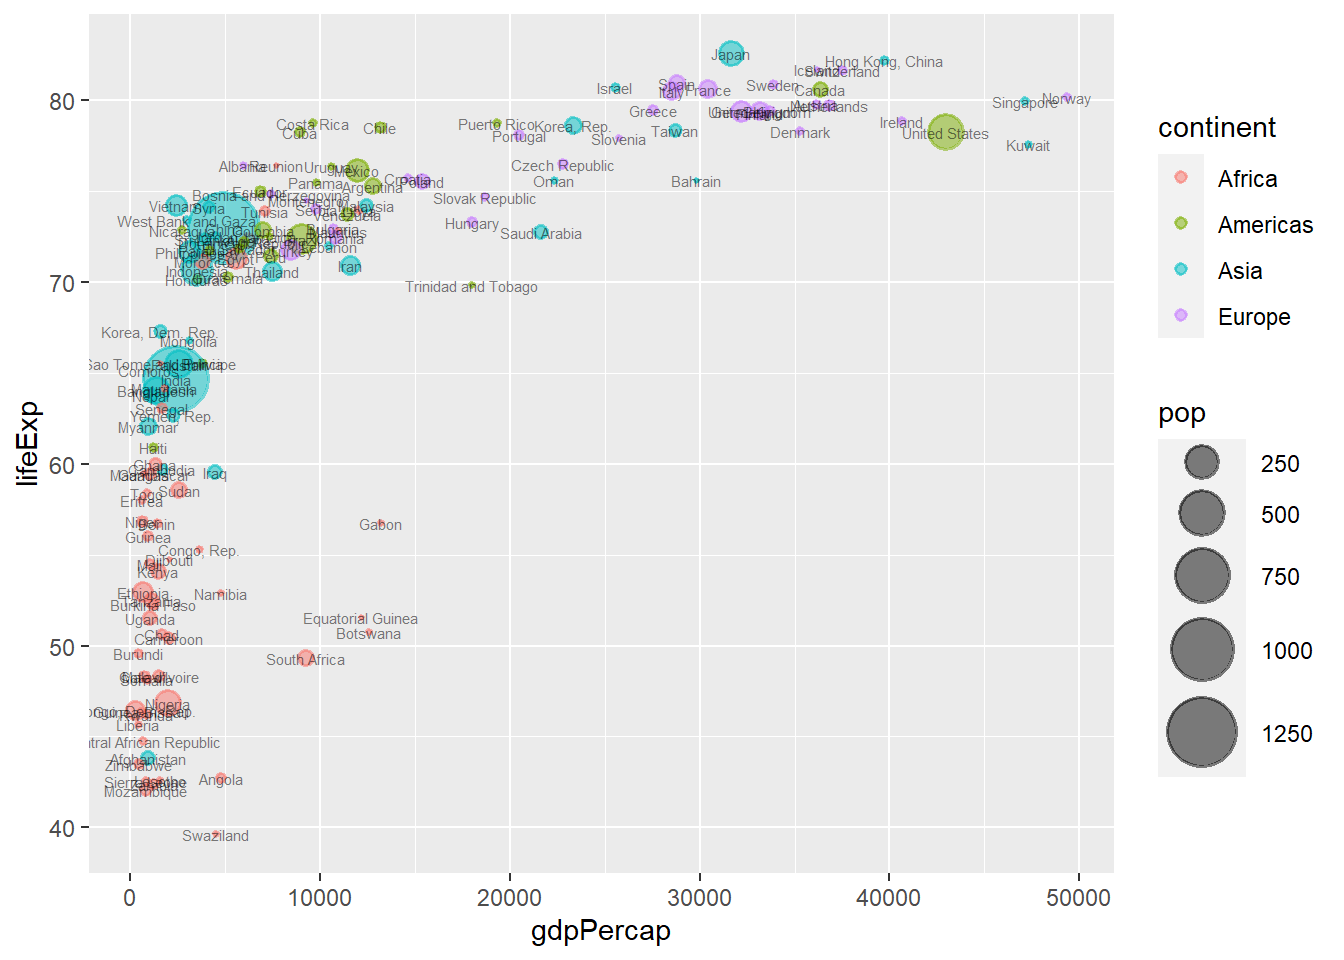
\includegraphics{04-tidyverser_files/figure-latex/unnamed-chunk-26-1.pdf}

\begin{Shaded}
\begin{Highlighting}[]


\CommentTok{\# reordering continent by population}
\NormalTok{pop\_cont}\SpecialCharTok{$}\NormalTok{continent }\OtherTok{\textless{}{-}} \FunctionTok{fct\_reorder}\NormalTok{(pop\_cont}\SpecialCharTok{$}\NormalTok{continent, pop\_cont}\SpecialCharTok{$}\NormalTok{pop, }\AttributeTok{.desc =} \ConstantTok{TRUE}\NormalTok{)}
\FunctionTok{levels}\NormalTok{(pop\_cont}\SpecialCharTok{$}\NormalTok{continent)}
\CommentTok{\#\textgreater{} [1] "Asia"     "Africa"   "Americas" "Europe"   "Oceania"}

\CommentTok{\# sorting data frame by continent}
\NormalTok{pop\_cont }\OtherTok{\textless{}{-}} \FunctionTok{with}\NormalTok{(pop\_cont, pop\_cont[}\FunctionTok{order}\NormalTok{(continent),])}
\NormalTok{pop\_cont}
\CommentTok{\#\textgreater{}   continent        pop}
\CommentTok{\#\textgreater{} 3      Asia 3811953827}
\CommentTok{\#\textgreater{} 1    Africa  929539692}
\CommentTok{\#\textgreater{} 2  Americas  898871184}
\CommentTok{\#\textgreater{} 4    Europe  586098529}
\CommentTok{\#\textgreater{} 5   Oceania   24549947}

\CommentTok{\# plotting barplot}
\FunctionTok{with}\NormalTok{(pop\_cont, }\FunctionTok{barplot}\NormalTok{(pop}\SpecialCharTok{/}\FloatTok{1e6}\NormalTok{, }\AttributeTok{names.arg =}\NormalTok{ continent))}
\end{Highlighting}
\end{Shaded}

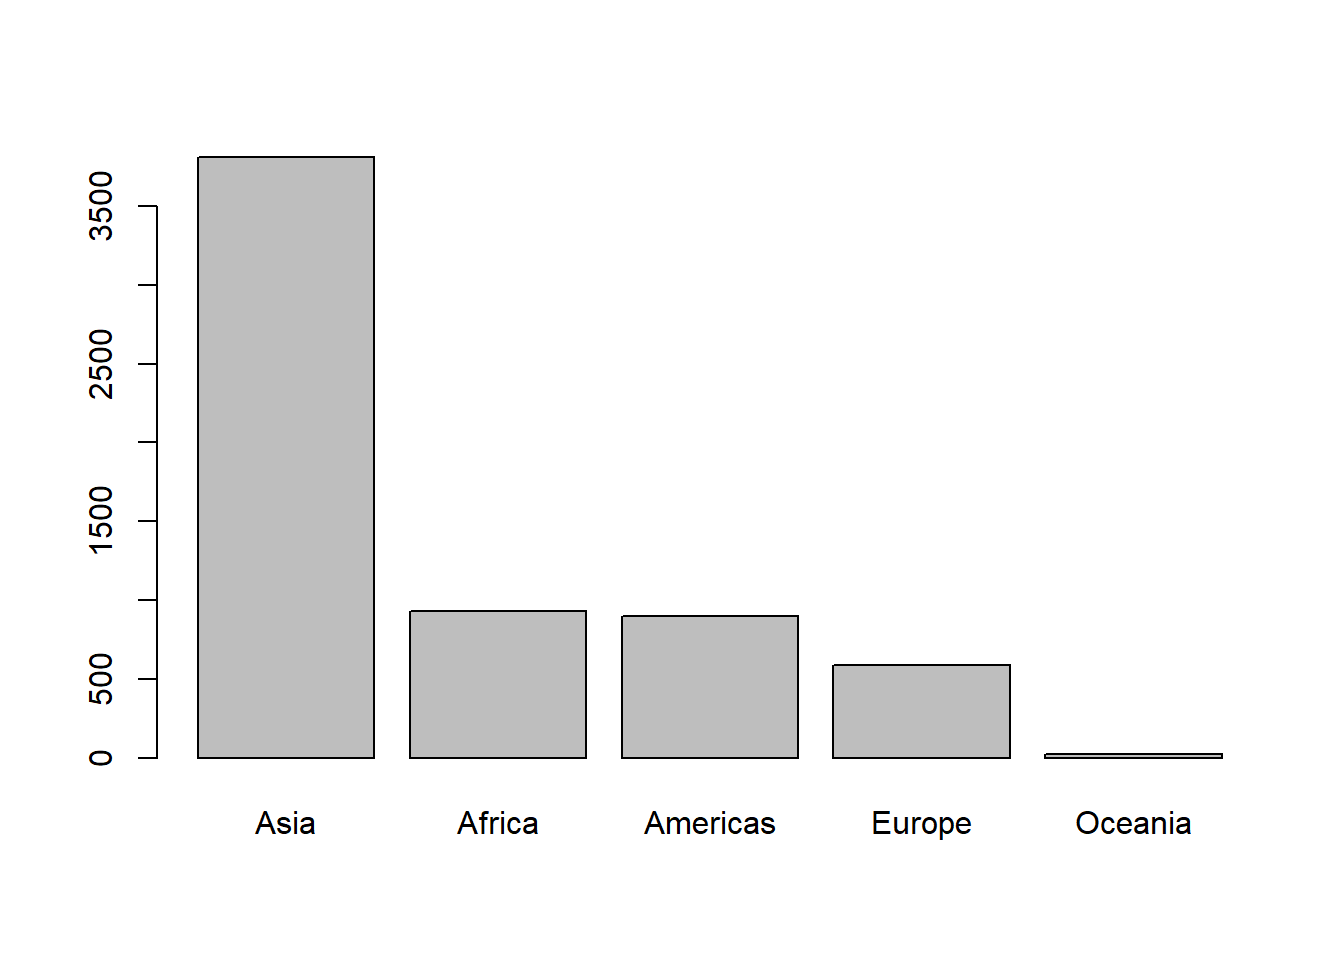
\includegraphics{04-tidyverser_files/figure-latex/unnamed-chunk-26-2.pdf}

\begin{Shaded}
\begin{Highlighting}[]

\CommentTok{\# producing an ascending bar chart}
\NormalTok{pop\_cont}\SpecialCharTok{$}\NormalTok{continent }\OtherTok{\textless{}{-}} \FunctionTok{fct\_reorder}\NormalTok{(pop\_cont}\SpecialCharTok{$}\NormalTok{continent, pop\_cont}\SpecialCharTok{$}\NormalTok{pop, }\AttributeTok{.desc =} \ConstantTok{FALSE}\NormalTok{)}
\NormalTok{pop\_cont }\OtherTok{\textless{}{-}} \FunctionTok{with}\NormalTok{(pop\_cont, pop\_cont[}\FunctionTok{order}\NormalTok{(continent),])}
\FunctionTok{with}\NormalTok{(pop\_cont, }\FunctionTok{barplot}\NormalTok{(pop}\SpecialCharTok{/}\FloatTok{1e6}\NormalTok{, }\AttributeTok{names.arg =}\NormalTok{ continent))}
\end{Highlighting}
\end{Shaded}

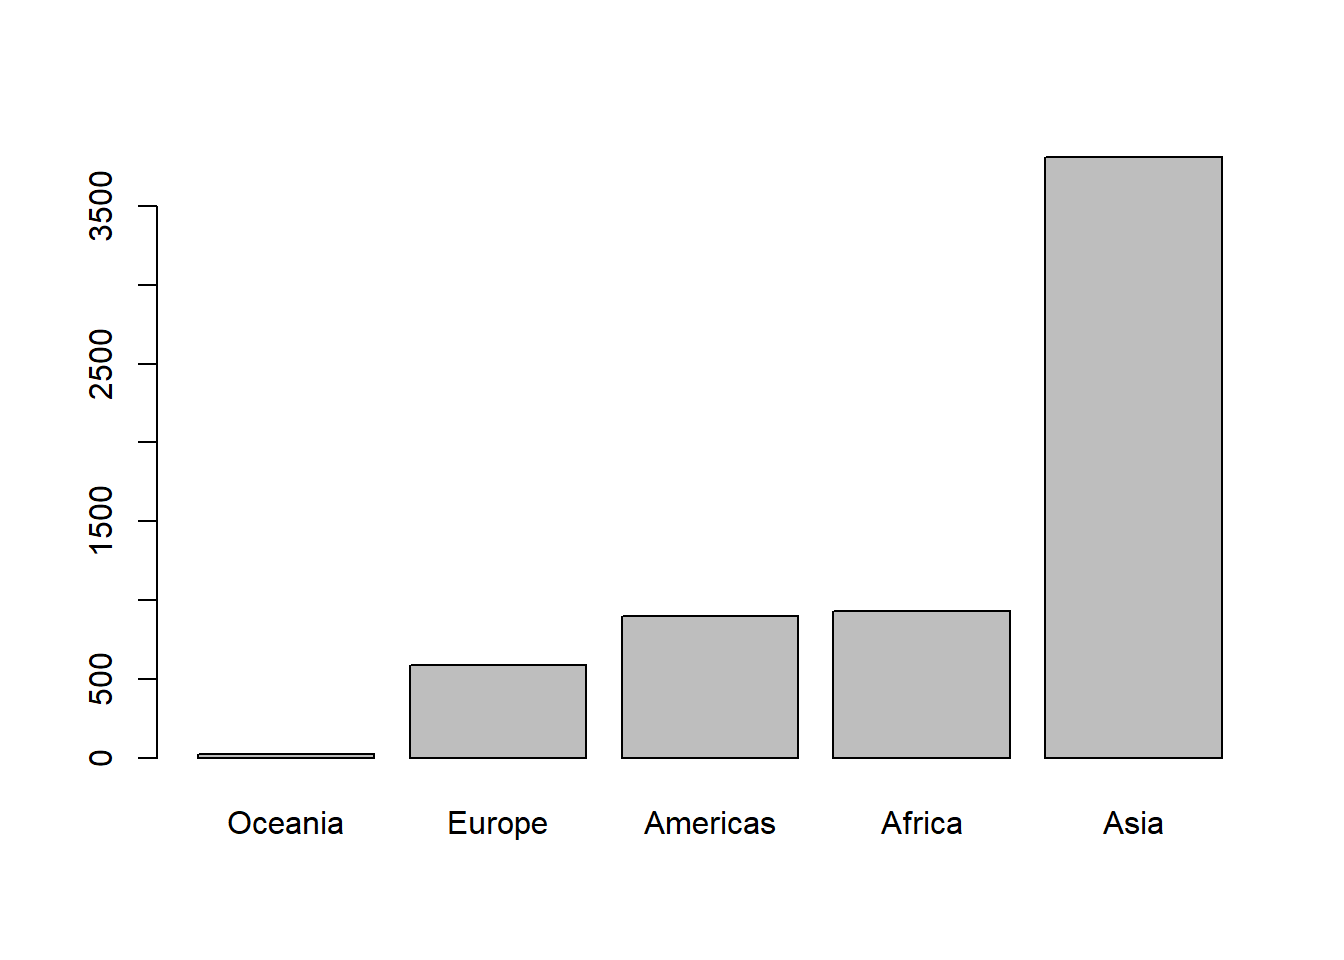
\includegraphics{04-tidyverser_files/figure-latex/unnamed-chunk-26-3.pdf}

\hypertarget{restructuring-levels-and-their-labels}{%
\subsection{Restructuring levels and their labels}\label{restructuring-levels-and-their-labels}}

\hypertarget{renaming-labels}{%
\subsubsection{Renaming labels}\label{renaming-labels}}

The function \texttt{fct\_recode()} is used to rename levels. It takes the form \texttt{new\_name\ =\ old\_name}.

\begin{Shaded}
\begin{Highlighting}[]
\FunctionTok{levels}\NormalTok{(}\FunctionTok{fct\_recode}\NormalTok{(gapminder\_2007}\SpecialCharTok{$}\NormalTok{continent, }\StringTok{\textquotesingle{}AS\textquotesingle{}} \OtherTok{=} \StringTok{\textquotesingle{}Asia\textquotesingle{}}\NormalTok{, }\StringTok{\textquotesingle{}Af\textquotesingle{}} \OtherTok{=} \StringTok{\textquotesingle{}Africa\textquotesingle{}}\NormalTok{, }\StringTok{\textquotesingle{}Eu\textquotesingle{}} \OtherTok{=} \StringTok{\textquotesingle{}Europe\textquotesingle{}}\NormalTok{))}
\CommentTok{\#\textgreater{} [1] "Americas" "Eu"       "Af"       "Oceania"  "AS"}
\end{Highlighting}
\end{Shaded}

\hypertarget{collapsing-levels}{%
\subsubsection{collapsing levels}\label{collapsing-levels}}

The function \texttt{fct\_collapse()} is used to collapse levels into a new one.

\begin{Shaded}
\begin{Highlighting}[]
\CommentTok{\# collapsing europe and africa into euroafrica}
\NormalTok{gapminder\_2007}\SpecialCharTok{$}\NormalTok{continent }\OtherTok{\textless{}{-}} 
  \FunctionTok{fct\_collapse}\NormalTok{(gapminder\_2007}\SpecialCharTok{$}\NormalTok{continent, }\AttributeTok{Euroafrica =} \FunctionTok{c}\NormalTok{(}\StringTok{\textquotesingle{}Africa\textquotesingle{}}\NormalTok{, }\StringTok{\textquotesingle{}Europe\textquotesingle{}}\NormalTok{))}
\FunctionTok{table}\NormalTok{(gapminder\_2007}\SpecialCharTok{$}\NormalTok{continent)}
\CommentTok{\#\textgreater{} }
\CommentTok{\#\textgreater{}   Americas Euroafrica    Oceania       Asia }
\CommentTok{\#\textgreater{}         25         82          2         33}

\CommentTok{\# population by continent}
\NormalTok{(pop\_cont }\OtherTok{\textless{}{-}} \FunctionTok{aggregate}\NormalTok{(pop }\SpecialCharTok{\textasciitilde{}}\NormalTok{ continent, gapminder\_2007, sum))}
\CommentTok{\#\textgreater{}    continent        pop}
\CommentTok{\#\textgreater{} 1   Americas  898871184}
\CommentTok{\#\textgreater{} 2 Euroafrica 1515638221}
\CommentTok{\#\textgreater{} 3    Oceania   24549947}
\CommentTok{\#\textgreater{} 4       Asia 3811953827}
\end{Highlighting}
\end{Shaded}

\hypertarget{combining-levels}{%
\subsubsection{combining levels}\label{combining-levels}}

The functions \texttt{fct\_lump()} and \texttt{fct\_lump\_min()} combines levels together based on the frequency of occurrence of each level.

\begin{Shaded}
\begin{Highlighting}[]
\CommentTok{\# combining the least frequent levels}
\NormalTok{gapminder\_2007 }\OtherTok{\textless{}{-}} \FunctionTok{subset}\NormalTok{(gapminder, year }\SpecialCharTok{==} \DecValTok{2007}\NormalTok{, }\SpecialCharTok{{-}}\DecValTok{3}\NormalTok{)}
\FunctionTok{table}\NormalTok{(}\FunctionTok{fct\_lump}\NormalTok{(gapminder\_2007}\SpecialCharTok{$}\NormalTok{continent))}
\CommentTok{\#\textgreater{} }
\CommentTok{\#\textgreater{} Africa   Asia Europe  Other }
\CommentTok{\#\textgreater{}     52     33     30     27}
\end{Highlighting}
\end{Shaded}

Using the arguments \texttt{n=} and \texttt{p=} we can specify the type of combining to perform; with positive values indicating combining rarest levels while negative values indicate combining most common levels.

\begin{Shaded}
\begin{Highlighting}[]
\CommentTok{\# combining all except the first most common}
\FunctionTok{table}\NormalTok{(}\FunctionTok{fct\_lump}\NormalTok{(gapminder\_2007}\SpecialCharTok{$}\NormalTok{continent, }\AttributeTok{n =} \DecValTok{1}\NormalTok{))}
\CommentTok{\#\textgreater{} }
\CommentTok{\#\textgreater{} Africa  Other }
\CommentTok{\#\textgreater{}     52     90}

\CommentTok{\# combining all except the first 2 most common}
\FunctionTok{table}\NormalTok{(}\FunctionTok{fct\_lump}\NormalTok{(gapminder\_2007}\SpecialCharTok{$}\NormalTok{continent, }\AttributeTok{n =} \DecValTok{2}\NormalTok{))}
\CommentTok{\#\textgreater{} }
\CommentTok{\#\textgreater{} Africa   Asia  Other }
\CommentTok{\#\textgreater{}     52     33     57}

\CommentTok{\# combining all except the first 3 most common}
\FunctionTok{table}\NormalTok{(}\FunctionTok{fct\_lump}\NormalTok{(gapminder\_2007}\SpecialCharTok{$}\NormalTok{continent, }\AttributeTok{n =} \DecValTok{3}\NormalTok{))}
\CommentTok{\#\textgreater{} }
\CommentTok{\#\textgreater{} Africa   Asia Europe  Other }
\CommentTok{\#\textgreater{}     52     33     30     27}

\CommentTok{\# combining all except the first rarest}
\FunctionTok{table}\NormalTok{(}\FunctionTok{fct\_lump}\NormalTok{(gapminder\_2007}\SpecialCharTok{$}\NormalTok{continent, }\AttributeTok{n =} \SpecialCharTok{{-}}\DecValTok{1}\NormalTok{))}
\CommentTok{\#\textgreater{} }
\CommentTok{\#\textgreater{} Oceania   Other }
\CommentTok{\#\textgreater{}       2     140}

\CommentTok{\# combining all except the first 2 rarest}
\FunctionTok{table}\NormalTok{(}\FunctionTok{fct\_lump}\NormalTok{(gapminder\_2007}\SpecialCharTok{$}\NormalTok{continent, }\AttributeTok{n =} \SpecialCharTok{{-}}\DecValTok{2}\NormalTok{))}
\CommentTok{\#\textgreater{} }
\CommentTok{\#\textgreater{} Americas  Oceania    Other }
\CommentTok{\#\textgreater{}       25        2      115}

\CommentTok{\# combining all except the first 3 rarest}
\FunctionTok{table}\NormalTok{(}\FunctionTok{fct\_lump}\NormalTok{(gapminder\_2007}\SpecialCharTok{$}\NormalTok{continent, }\AttributeTok{n =} \SpecialCharTok{{-}}\DecValTok{3}\NormalTok{))}
\CommentTok{\#\textgreater{} }
\CommentTok{\#\textgreater{} Americas   Europe  Oceania    Other }
\CommentTok{\#\textgreater{}       25       30        2       85}

\CommentTok{\# using prop positive}
\FunctionTok{table}\NormalTok{(}\FunctionTok{fct\_lump}\NormalTok{(gapminder\_2007}\SpecialCharTok{$}\NormalTok{continent, }\AttributeTok{prop =} \FloatTok{0.25}\NormalTok{))}
\CommentTok{\#\textgreater{} }
\CommentTok{\#\textgreater{} Africa  Other }
\CommentTok{\#\textgreater{}     52     90}
\FunctionTok{table}\NormalTok{(}\FunctionTok{fct\_lump}\NormalTok{(gapminder\_2007}\SpecialCharTok{$}\NormalTok{continent, }\AttributeTok{prop =} \FloatTok{0.22}\NormalTok{))}
\CommentTok{\#\textgreater{} }
\CommentTok{\#\textgreater{} Africa   Asia  Other }
\CommentTok{\#\textgreater{}     52     33     57}
\FunctionTok{table}\NormalTok{(}\FunctionTok{fct\_lump}\NormalTok{(gapminder\_2007}\SpecialCharTok{$}\NormalTok{continent, }\AttributeTok{prop =} \FloatTok{0.2}\NormalTok{))}
\CommentTok{\#\textgreater{} }
\CommentTok{\#\textgreater{} Africa   Asia Europe  Other }
\CommentTok{\#\textgreater{}     52     33     30     27}

\CommentTok{\# using prop negative}
\FunctionTok{table}\NormalTok{(}\FunctionTok{fct\_lump}\NormalTok{(gapminder\_2007}\SpecialCharTok{$}\NormalTok{continent, }\AttributeTok{prop =} \SpecialCharTok{{-}}\FloatTok{0.25}\NormalTok{))}
\CommentTok{\#\textgreater{} }
\CommentTok{\#\textgreater{} Americas     Asia   Europe  Oceania    Other }
\CommentTok{\#\textgreater{}       25       33       30        2       52}
\FunctionTok{table}\NormalTok{(}\FunctionTok{fct\_lump}\NormalTok{(gapminder\_2007}\SpecialCharTok{$}\NormalTok{continent, }\AttributeTok{prop =} \SpecialCharTok{{-}}\FloatTok{0.22}\NormalTok{))}
\CommentTok{\#\textgreater{} }
\CommentTok{\#\textgreater{} Americas   Europe  Oceania    Other }
\CommentTok{\#\textgreater{}       25       30        2       85}
\FunctionTok{table}\NormalTok{(}\FunctionTok{fct\_lump}\NormalTok{(gapminder\_2007}\SpecialCharTok{$}\NormalTok{continent, }\AttributeTok{prop =} \SpecialCharTok{{-}}\FloatTok{0.2}\NormalTok{))}
\CommentTok{\#\textgreater{} }
\CommentTok{\#\textgreater{} Americas  Oceania    Other }
\CommentTok{\#\textgreater{}       25        2      115}
\end{Highlighting}
\end{Shaded}

With \texttt{fct\_lump\_min()} combining is done based on whether a threshold declared by the min argument is met.

\begin{Shaded}
\begin{Highlighting}[]
\FunctionTok{table}\NormalTok{(gapminder\_2007}\SpecialCharTok{$}\NormalTok{continent)}
\CommentTok{\#\textgreater{} }
\CommentTok{\#\textgreater{}   Africa Americas     Asia   Europe  Oceania }
\CommentTok{\#\textgreater{}       52       25       33       30        2}

\CommentTok{\# combining levels with less than 25 counts}
\FunctionTok{table}\NormalTok{(}\FunctionTok{fct\_lump\_min}\NormalTok{(gapminder\_2007}\SpecialCharTok{$}\NormalTok{continent, }\AttributeTok{min =} \DecValTok{25}\NormalTok{))}
\CommentTok{\#\textgreater{} }
\CommentTok{\#\textgreater{}   Africa Americas     Asia   Europe    Other }
\CommentTok{\#\textgreater{}       52       25       33       30        2}

\CommentTok{\# combining levels with less than 30 counts}
\FunctionTok{table}\NormalTok{(}\FunctionTok{fct\_lump\_min}\NormalTok{(gapminder\_2007}\SpecialCharTok{$}\NormalTok{continent, }\AttributeTok{min =} \DecValTok{30}\NormalTok{))}
\CommentTok{\#\textgreater{} }
\CommentTok{\#\textgreater{} Africa   Asia Europe  Other }
\CommentTok{\#\textgreater{}     52     33     30     27}

\CommentTok{\# combining levels with less than 33 counts}
\FunctionTok{table}\NormalTok{(}\FunctionTok{fct\_lump\_min}\NormalTok{(gapminder\_2007}\SpecialCharTok{$}\NormalTok{continent, }\AttributeTok{min =} \DecValTok{33}\NormalTok{))}
\CommentTok{\#\textgreater{} }
\CommentTok{\#\textgreater{} Africa   Asia  Other }
\CommentTok{\#\textgreater{}     52     33     57}
\end{Highlighting}
\end{Shaded}

\hypertarget{remove-and-add-levels}{%
\subsection{Remove and add levels}\label{remove-and-add-levels}}

\hypertarget{dropping-levels-1}{%
\subsubsection{dropping levels}\label{dropping-levels-1}}

The function \texttt{fct\_other()} will drop levels and replace them with the argument other\_level = other by default.

\begin{Shaded}
\begin{Highlighting}[]
\CommentTok{\# keeping asia and europe }
\FunctionTok{table}\NormalTok{(}\FunctionTok{fct\_other}\NormalTok{(gapminder\_2007}\SpecialCharTok{$}\NormalTok{continent, }\AttributeTok{keep =} \FunctionTok{c}\NormalTok{(}\StringTok{\textquotesingle{}Asia\textquotesingle{}}\NormalTok{, }\StringTok{\textquotesingle{}Europe\textquotesingle{}}\NormalTok{)))}
\CommentTok{\#\textgreater{} }
\CommentTok{\#\textgreater{}   Asia Europe  Other }
\CommentTok{\#\textgreater{}     33     30     79}

\CommentTok{\# dropping asia and europe}
\FunctionTok{table}\NormalTok{(}\FunctionTok{fct\_other}\NormalTok{(gapminder\_2007}\SpecialCharTok{$}\NormalTok{continent, }\AttributeTok{drop =} \FunctionTok{c}\NormalTok{(}\StringTok{\textquotesingle{}Asia\textquotesingle{}}\NormalTok{, }\StringTok{\textquotesingle{}Europe\textquotesingle{}}\NormalTok{)))}
\CommentTok{\#\textgreater{} }
\CommentTok{\#\textgreater{}   Africa Americas  Oceania    Other }
\CommentTok{\#\textgreater{}       52       25        2       63}

\CommentTok{\# replacing other continents with nonEurasia}
\FunctionTok{table}\NormalTok{(}\FunctionTok{fct\_other}\NormalTok{(gapminder\_2007}\SpecialCharTok{$}\NormalTok{continent, }
                \AttributeTok{keep =} \FunctionTok{c}\NormalTok{(}\StringTok{\textquotesingle{}Asia\textquotesingle{}}\NormalTok{, }\StringTok{\textquotesingle{}Europe\textquotesingle{}}\NormalTok{), }
                \AttributeTok{other\_level =} \StringTok{\textquotesingle{}nonEurasia\textquotesingle{}}\NormalTok{))}
\CommentTok{\#\textgreater{} }
\CommentTok{\#\textgreater{}       Asia     Europe nonEurasia }
\CommentTok{\#\textgreater{}         33         30         79}

\CommentTok{\# replacing europe and asia with Eurasia}
\FunctionTok{table}\NormalTok{(}\FunctionTok{fct\_other}\NormalTok{(gapminder\_2007}\SpecialCharTok{$}\NormalTok{continent, }
                \AttributeTok{drop =} \FunctionTok{c}\NormalTok{(}\StringTok{\textquotesingle{}Asia\textquotesingle{}}\NormalTok{, }\StringTok{\textquotesingle{}Europe\textquotesingle{}}\NormalTok{), }
                \AttributeTok{other\_level =} \StringTok{\textquotesingle{}Eurasia\textquotesingle{}}\NormalTok{))}
\CommentTok{\#\textgreater{} }
\CommentTok{\#\textgreater{}   Africa Americas  Oceania  Eurasia }
\CommentTok{\#\textgreater{}       52       25        2       63}
\end{Highlighting}
\end{Shaded}

\hypertarget{dropping-unused-levels}{%
\subsection{dropping unused levels}\label{dropping-unused-levels}}

The function \texttt{fct\_drop()} is used to drop unused levels. Unused levels are usually a problem while plotting as they appear on the graph though they contain no data.

\begin{Shaded}
\begin{Highlighting}[]
\CommentTok{\# dropping Oceania}
\NormalTok{gapminder\_oc }\OtherTok{\textless{}{-}} \FunctionTok{subset}\NormalTok{(gapminder\_2007, continent }\SpecialCharTok{!=} \StringTok{\textquotesingle{}Oceania\textquotesingle{}}\NormalTok{)}
\FunctionTok{table}\NormalTok{(gapminder\_oc}\SpecialCharTok{$}\NormalTok{continent)}
\CommentTok{\#\textgreater{} }
\CommentTok{\#\textgreater{}   Africa Americas     Asia   Europe  Oceania }
\CommentTok{\#\textgreater{}       52       25       33       30        0}
\CommentTok{\# Because the level Oceania has not been dropped, it appears on the above plot.}
\FunctionTok{plot}\NormalTok{(gapminder\_oc}\SpecialCharTok{$}\NormalTok{continent)}
\end{Highlighting}
\end{Shaded}

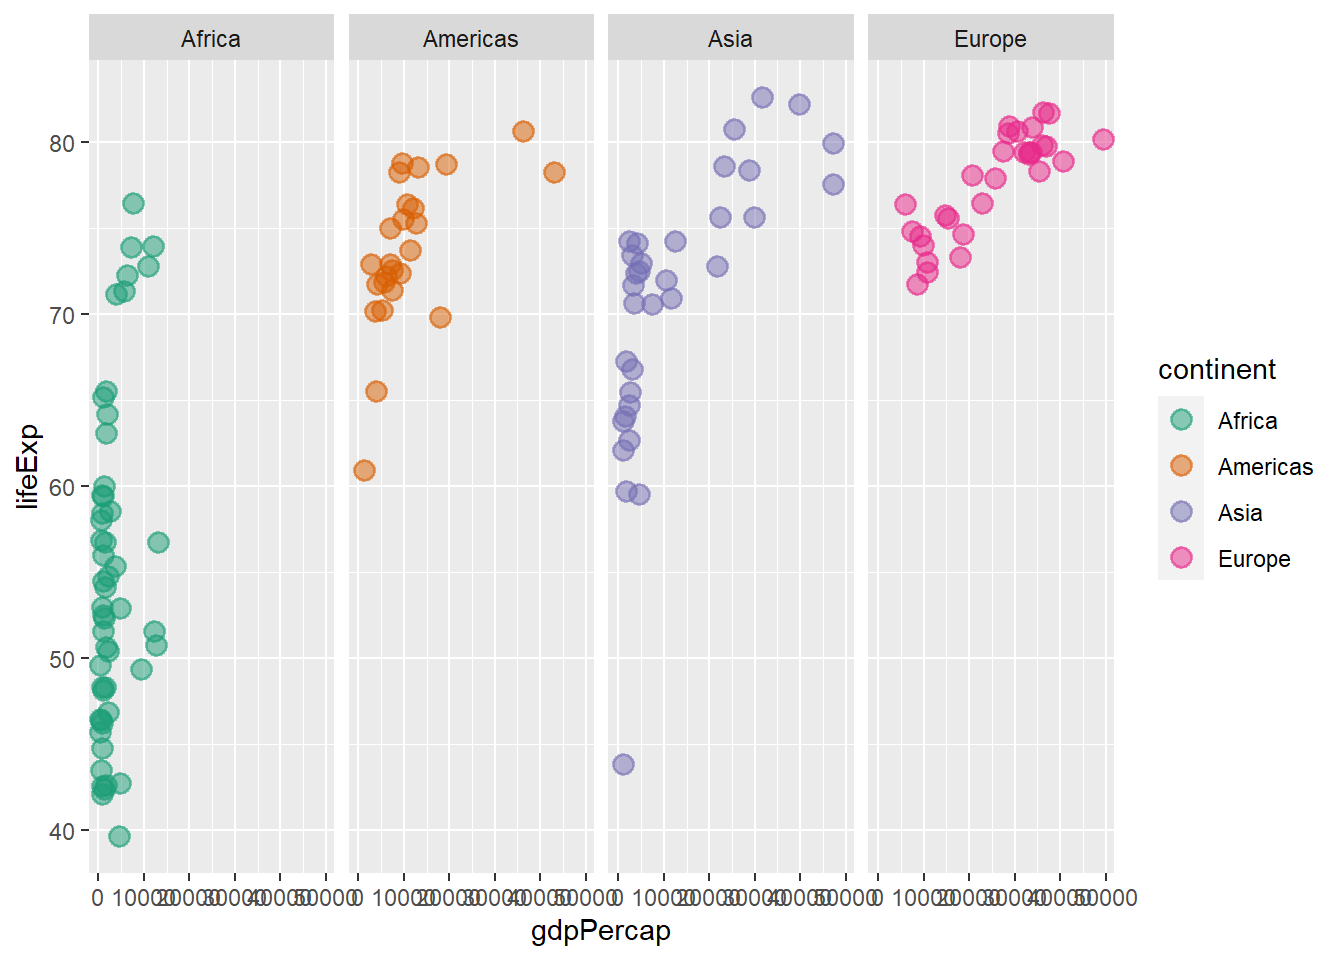
\includegraphics{04-tidyverser_files/figure-latex/unnamed-chunk-33-1.pdf}

\begin{Shaded}
\begin{Highlighting}[]

\CommentTok{\# dropping unused level}
\FunctionTok{table}\NormalTok{(}\FunctionTok{fct\_drop}\NormalTok{(gapminder\_oc}\SpecialCharTok{$}\NormalTok{continent))}
\CommentTok{\#\textgreater{} }
\CommentTok{\#\textgreater{}   Africa Americas     Asia   Europe }
\CommentTok{\#\textgreater{}       52       25       33       30}
\FunctionTok{plot}\NormalTok{(}\FunctionTok{fct\_drop}\NormalTok{(gapminder\_oc}\SpecialCharTok{$}\NormalTok{continent))}
\end{Highlighting}
\end{Shaded}

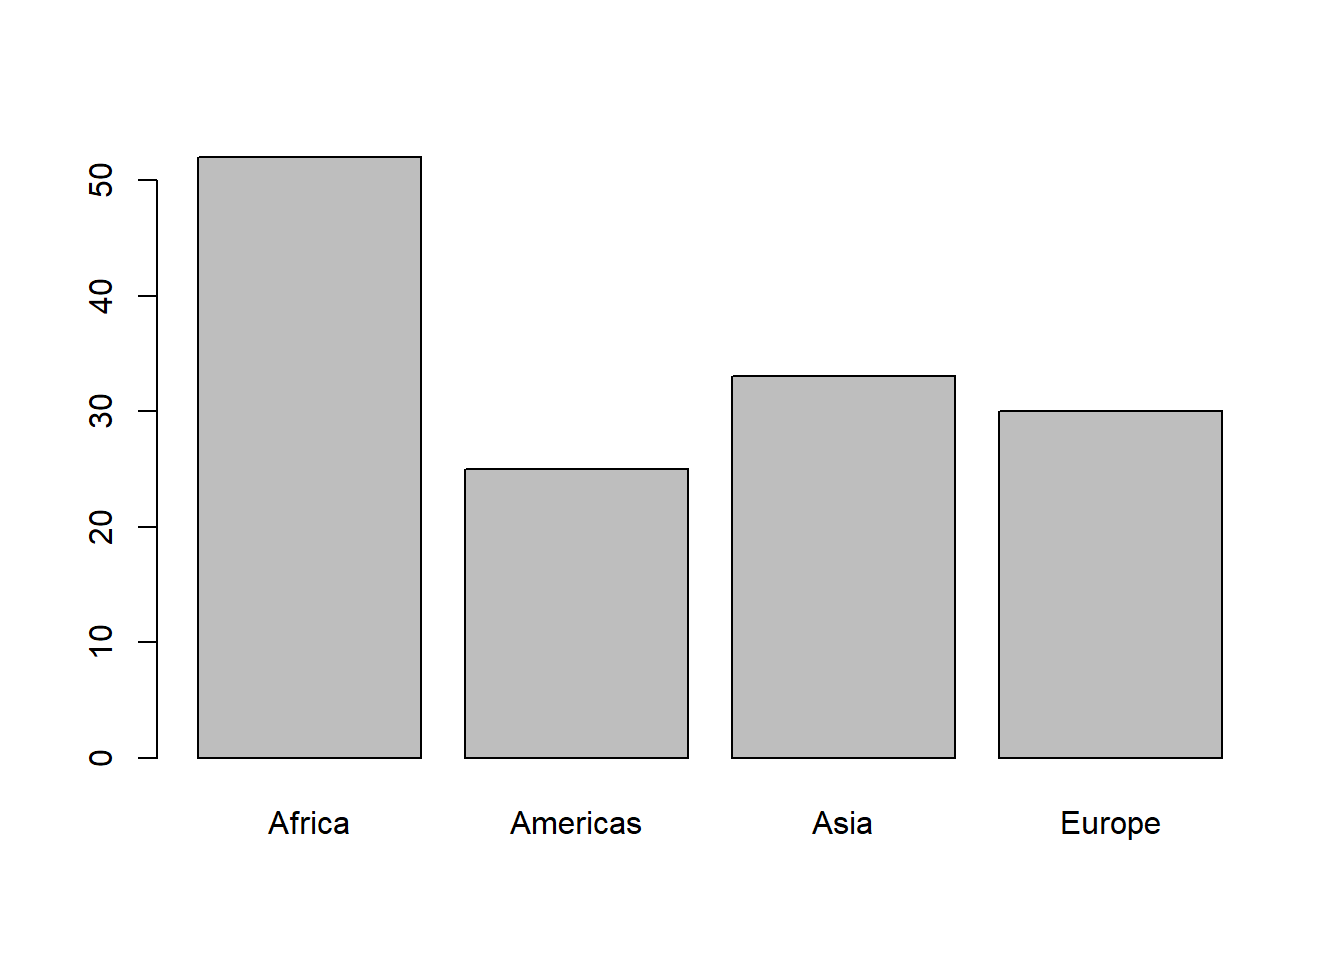
\includegraphics{04-tidyverser_files/figure-latex/unnamed-chunk-33-2.pdf}

\hypertarget{adding-levels}{%
\subsubsection{adding levels}\label{adding-levels}}

The function \texttt{fct\_expand()} is used to add levels.

\begin{Shaded}
\begin{Highlighting}[]
\CommentTok{\# adding the level arctic}
\FunctionTok{table}\NormalTok{(}\FunctionTok{fct\_expand}\NormalTok{(gapminder\_oc}\SpecialCharTok{$}\NormalTok{continent, }\StringTok{\textquotesingle{}arctic\textquotesingle{}}\NormalTok{))}
\CommentTok{\#\textgreater{} }
\CommentTok{\#\textgreater{}   Africa Americas     Asia   Europe  Oceania   arctic }
\CommentTok{\#\textgreater{}       52       25       33       30        0        0}

\CommentTok{\# adding the levels arctic and antarctica}
\FunctionTok{table}\NormalTok{(}\FunctionTok{fct\_expand}\NormalTok{(gapminder\_oc}\SpecialCharTok{$}\NormalTok{continent, }\FunctionTok{c}\NormalTok{(}\StringTok{\textquotesingle{}arctic\textquotesingle{}}\NormalTok{, }\StringTok{\textquotesingle{}antarctica\textquotesingle{}}\NormalTok{)))}
\CommentTok{\#\textgreater{} }
\CommentTok{\#\textgreater{}     Africa   Americas       Asia     Europe    Oceania }
\CommentTok{\#\textgreater{}         52         25         33         30          0 }
\CommentTok{\#\textgreater{}     arctic antarctica }
\CommentTok{\#\textgreater{}          0          0}
\CommentTok{\# newly added levels appear on the plot though they have no data}
\FunctionTok{plot}\NormalTok{(}\FunctionTok{fct\_expand}\NormalTok{(gapminder\_oc}\SpecialCharTok{$}\NormalTok{continent, }\FunctionTok{c}\NormalTok{(}\StringTok{\textquotesingle{}arctic\textquotesingle{}}\NormalTok{, }\StringTok{\textquotesingle{}antarctica\textquotesingle{}}\NormalTok{)))}
\end{Highlighting}
\end{Shaded}

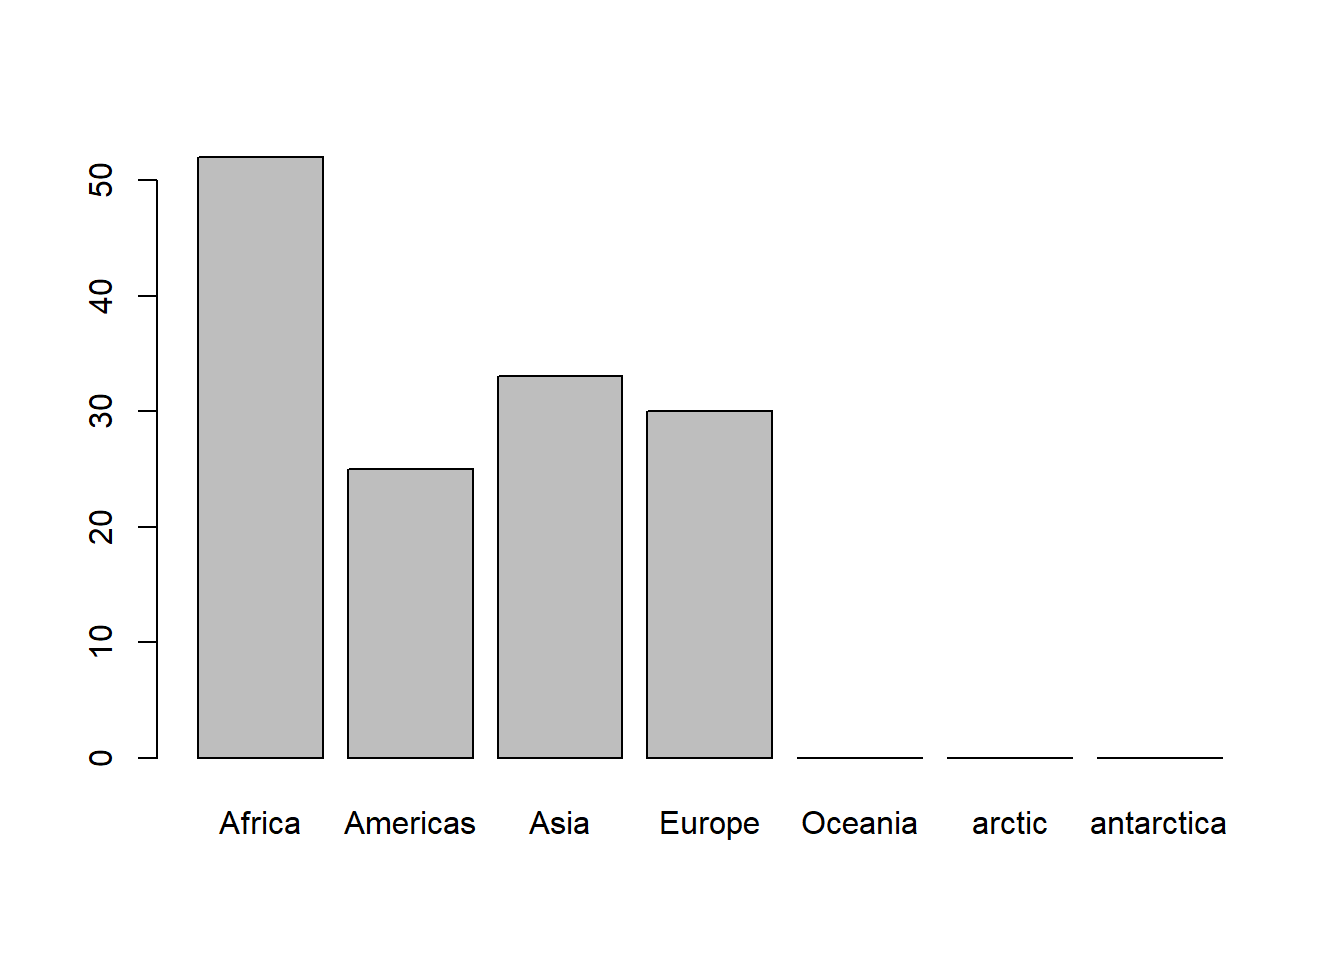
\includegraphics{04-tidyverser_files/figure-latex/unnamed-chunk-34-1.pdf}

\hypertarget{data-manipulation-with-dplyr-and-tidyr}{%
\section{Data Manipulation with dplyr and tidyr}\label{data-manipulation-with-dplyr-and-tidyr}}

The package \textbf{dplyr} is one of the core packages in a group of packages known as the tidyverse. It was developed and released in 2014 by Hadley Wickham and others. \textbf{dplyr} is meant to be for data manipulation what \textbf{ggplot2} is for data visualization, that is the grammar of data manipulation. It focuses solely on data frame manipulation and transformation using a set of verbs (functions) which are consistent and easy to understand.

Since \textbf{dyplr} belongs to the tidyverse world, it can be installed either by installing tidyverse or by installing \textbf{dplyr} itself.

\hypertarget{rename-columns-and-rows}{%
\subsection{Rename columns and rows}\label{rename-columns-and-rows}}

\hypertarget{tr-col-names}{%
\subsubsection{Renaming columns}\label{tr-col-names}}

The function \texttt{rename()} is used to rename columns.

\texttt{rename(new\_name\ =\ old\_name)}

\begin{Shaded}
\begin{Highlighting}[]
\FunctionTok{library}\NormalTok{(readr)}
\FunctionTok{library}\NormalTok{(dplyr)}
\FunctionTok{library}\NormalTok{(gapminder)}

\CommentTok{\# loading data}
\FunctionTok{data}\NormalTok{(gapminder)}
\CommentTok{\# get column names}
\FunctionTok{names}\NormalTok{(gapminder)}
\CommentTok{\#\textgreater{} [1] "country"   "continent" "year"      "lifeExp"  }
\CommentTok{\#\textgreater{} [5] "pop"       "gdpPercap"}

\CommentTok{\# set column names}
\NormalTok{gapminder }\OtherTok{\textless{}{-}} \FunctionTok{rename}\NormalTok{(gapminder, }
                    \AttributeTok{Country =}\NormalTok{ country, }
                    \AttributeTok{Continent =}\NormalTok{ continent, }
                    \AttributeTok{Year =}\NormalTok{ year, }
                    \StringTok{\textasciigrave{}}\AttributeTok{Life Expectancy}\StringTok{\textasciigrave{}} \OtherTok{=}\NormalTok{ lifeExp, }
                    \AttributeTok{Population =}\NormalTok{ pop, }
                    \StringTok{\textasciigrave{}}\AttributeTok{GDP per Capita}\StringTok{\textasciigrave{}} \OtherTok{=}\NormalTok{ gdpPercap)}
\CommentTok{\# get column names}
\FunctionTok{colnames}\NormalTok{(gapminder)}
\CommentTok{\#\textgreater{} [1] "Country"         "Continent"       "Year"           }
\CommentTok{\#\textgreater{} [4] "Life Expectancy" "Population"      "GDP per Capita"}
\end{Highlighting}
\end{Shaded}

\hypertarget{renaming-rows}{%
\subsubsection{Renaming rows}\label{renaming-rows}}

Tibble does not support row names. See \href{tidyverse-r.html\#row-names}{this}.

\hypertarget{select-columns-and-filter-rows}{%
\subsection{Select columns and filter rows}\label{select-columns-and-filter-rows}}

\hypertarget{tr-filter-cols}{%
\subsubsection{Selecting and dropping columns}\label{tr-filter-cols}}

The function \texttt{select()} is used to select and rename columns.

\begin{Shaded}
\begin{Highlighting}[]
\CommentTok{\# preparing data}
\NormalTok{column\_names }\OtherTok{\textless{}{-}} \FunctionTok{c}\NormalTok{(}\StringTok{\textquotesingle{}Rank\textquotesingle{}}\NormalTok{, }\StringTok{\textquotesingle{}Title\textquotesingle{}}\NormalTok{, }\StringTok{\textquotesingle{}Genre\textquotesingle{}}\NormalTok{, }\StringTok{\textquotesingle{}Description\textquotesingle{}}\NormalTok{, }\StringTok{\textquotesingle{}Director\textquotesingle{}}\NormalTok{, }\StringTok{\textquotesingle{}Actors\textquotesingle{}}\NormalTok{, }
                  \StringTok{\textquotesingle{}Year\textquotesingle{}}\NormalTok{, }\StringTok{\textquotesingle{}Runtime\textquotesingle{}}\NormalTok{, }\StringTok{\textquotesingle{}Rating\textquotesingle{}}\NormalTok{, }\StringTok{\textquotesingle{}Votes\textquotesingle{}}\NormalTok{, }\StringTok{\textquotesingle{}Revenue\textquotesingle{}}\NormalTok{, }\StringTok{\textquotesingle{}Metascore\textquotesingle{}}\NormalTok{)}
\NormalTok{mov }\OtherTok{\textless{}{-}} \FunctionTok{read.table}\NormalTok{(}\AttributeTok{file =} \StringTok{"data/IMDB{-}Movie{-}Data.csv"}\NormalTok{, }\AttributeTok{header =}\NormalTok{ T, }\AttributeTok{sep =} \StringTok{","}\NormalTok{, }\AttributeTok{dec =} \StringTok{"."}\NormalTok{, }\AttributeTok{fileEncoding =} \StringTok{"UTF{-}8"}\NormalTok{, }\AttributeTok{quote =} \StringTok{"}\SpecialCharTok{\textbackslash{}"}\StringTok{"}\NormalTok{,}
                  \AttributeTok{comment.char =} \StringTok{""}\NormalTok{)}
\FunctionTok{head}\NormalTok{(mov, }\DecValTok{3}\NormalTok{)}
\CommentTok{\#\textgreater{}   Rank                   Title                    Genre}
\CommentTok{\#\textgreater{} 1    1 Guardians of the Galaxy  Action,Adventure,Sci{-}Fi}
\CommentTok{\#\textgreater{} 2    2              Prometheus Adventure,Mystery,Sci{-}Fi}
\CommentTok{\#\textgreater{} 3    3                   Split          Horror,Thriller}
\CommentTok{\#\textgreater{}                                                                                                                                                     Description}
\CommentTok{\#\textgreater{} 1                               A group of intergalactic criminals are forced to work together to stop a fanatical warrior from taking control of the universe.}
\CommentTok{\#\textgreater{} 2                               Following clues to the origin of mankind, a team finds a structure on a distant moon, but they soon realize they are not alone.}
\CommentTok{\#\textgreater{} 3 Three girls are kidnapped by a man with a diagnosed 23 distinct personalities. They must try to escape before the apparent emergence of a frightful new 24th.}
\CommentTok{\#\textgreater{}             Director}
\CommentTok{\#\textgreater{} 1         James Gunn}
\CommentTok{\#\textgreater{} 2       Ridley Scott}
\CommentTok{\#\textgreater{} 3 M. Night Shyamalan}
\CommentTok{\#\textgreater{}                                                                    Actors}
\CommentTok{\#\textgreater{} 1                    Chris Pratt, Vin Diesel, Bradley Cooper, Zoe Saldana}
\CommentTok{\#\textgreater{} 2 Noomi Rapace, Logan Marshall{-}Green, Michael Fassbender, Charlize Theron}
\CommentTok{\#\textgreater{} 3        James McAvoy, Anya Taylor{-}Joy, Haley Lu Richardson, Jessica Sula}
\CommentTok{\#\textgreater{}   Year Runtime..Minutes. Rating  Votes Revenue..Millions.}
\CommentTok{\#\textgreater{} 1 2014               121    8.1 757074             333.13}
\CommentTok{\#\textgreater{} 2 2012               124    7.0 485820             126.46}
\CommentTok{\#\textgreater{} 3 2016               117    7.3 157606             138.12}
\CommentTok{\#\textgreater{}   Metascore}
\CommentTok{\#\textgreater{} 1        76}
\CommentTok{\#\textgreater{} 2        65}
\CommentTok{\#\textgreater{} 3        62}
\FunctionTok{names}\NormalTok{(mov) }\OtherTok{\textless{}{-}} \FunctionTok{c}\NormalTok{(}\StringTok{\textquotesingle{}Rank\textquotesingle{}}\NormalTok{, }\StringTok{\textquotesingle{}Title\textquotesingle{}}\NormalTok{, }\StringTok{\textquotesingle{}Genre\textquotesingle{}}\NormalTok{, }\StringTok{\textquotesingle{}Description\textquotesingle{}}\NormalTok{, }\StringTok{\textquotesingle{}Director\textquotesingle{}}\NormalTok{, }\StringTok{\textquotesingle{}Actors\textquotesingle{}}\NormalTok{, }
                  \StringTok{\textquotesingle{}Year\textquotesingle{}}\NormalTok{, }\StringTok{\textquotesingle{}Runtime\textquotesingle{}}\NormalTok{, }\StringTok{\textquotesingle{}Rating\textquotesingle{}}\NormalTok{, }\StringTok{\textquotesingle{}Votes\textquotesingle{}}\NormalTok{, }\StringTok{\textquotesingle{}Revenue\textquotesingle{}}\NormalTok{, }\StringTok{\textquotesingle{}Metascore\textquotesingle{}}\NormalTok{)}


\CommentTok{\# selecting columns by column names}
\NormalTok{movies }\OtherTok{\textless{}{-}} \FunctionTok{select}\NormalTok{(mov, }\FunctionTok{c}\NormalTok{(}\StringTok{\textquotesingle{}Title\textquotesingle{}}\NormalTok{, }\StringTok{\textquotesingle{}Year\textquotesingle{}}\NormalTok{, }\StringTok{\textquotesingle{}Revenue\textquotesingle{}}\NormalTok{, }\StringTok{\textquotesingle{}Metascore\textquotesingle{}}\NormalTok{))}
\FunctionTok{head}\NormalTok{(movies, }\DecValTok{3}\NormalTok{)}
\CommentTok{\#\textgreater{}                     Title Year Revenue Metascore}
\CommentTok{\#\textgreater{} 1 Guardians of the Galaxy 2014  333.13        76}
\CommentTok{\#\textgreater{} 2              Prometheus 2012  126.46        65}
\CommentTok{\#\textgreater{} 3                   Split 2016  138.12        62}

\CommentTok{\# columns can be passed directly without quotation marks}
\NormalTok{movies }\OtherTok{\textless{}{-}} \FunctionTok{select}\NormalTok{(mov, Title, Year, Revenue, Metascore)}
\FunctionTok{head}\NormalTok{(movies, }\DecValTok{3}\NormalTok{)}
\CommentTok{\#\textgreater{}                     Title Year Revenue Metascore}
\CommentTok{\#\textgreater{} 1 Guardians of the Galaxy 2014  333.13        76}
\CommentTok{\#\textgreater{} 2              Prometheus 2012  126.46        65}
\CommentTok{\#\textgreater{} 3                   Split 2016  138.12        62}

\CommentTok{\# renaming column}
\NormalTok{movies }\OtherTok{\textless{}{-}} \FunctionTok{select}\NormalTok{(mov, }
\NormalTok{                 Title, }
                 \StringTok{\textasciigrave{}}\AttributeTok{Release Year}\StringTok{\textasciigrave{}} \OtherTok{=}\NormalTok{ Year, }
                 \StringTok{\textasciigrave{}}\AttributeTok{Revenue in Millions}\StringTok{\textasciigrave{}} \OtherTok{=}\NormalTok{ Revenue, }
\NormalTok{                 Metascore)}
\FunctionTok{head}\NormalTok{(movies, }\DecValTok{3}\NormalTok{)}
\CommentTok{\#\textgreater{}                     Title Release Year Revenue in Millions}
\CommentTok{\#\textgreater{} 1 Guardians of the Galaxy         2014              333.13}
\CommentTok{\#\textgreater{} 2              Prometheus         2012              126.46}
\CommentTok{\#\textgreater{} 3                   Split         2016              138.12}
\CommentTok{\#\textgreater{}   Metascore}
\CommentTok{\#\textgreater{} 1        76}
\CommentTok{\#\textgreater{} 2        65}
\CommentTok{\#\textgreater{} 3        62}

\CommentTok{\# selecting columns by position}
\NormalTok{movies }\OtherTok{\textless{}{-}} \FunctionTok{select}\NormalTok{(mov, }\DecValTok{2}\NormalTok{, }\DecValTok{7}\NormalTok{, }\DecValTok{11}\NormalTok{, }\DecValTok{12}\NormalTok{)}
\FunctionTok{head}\NormalTok{(movies, }\DecValTok{3}\NormalTok{)}
\CommentTok{\#\textgreater{}                     Title Year Revenue Metascore}
\CommentTok{\#\textgreater{} 1 Guardians of the Galaxy 2014  333.13        76}
\CommentTok{\#\textgreater{} 2              Prometheus 2012  126.46        65}
\CommentTok{\#\textgreater{} 3                   Split 2016  138.12        62}

\CommentTok{\# selecting columns by sequencing}
\NormalTok{movies }\OtherTok{\textless{}{-}} \FunctionTok{select}\NormalTok{(mov, }\DecValTok{7}\SpecialCharTok{:}\DecValTok{12}\NormalTok{)}
\FunctionTok{head}\NormalTok{(movies, }\DecValTok{3}\NormalTok{)}
\CommentTok{\#\textgreater{}   Year Runtime Rating  Votes Revenue Metascore}
\CommentTok{\#\textgreater{} 1 2014     121    8.1 757074  333.13        76}
\CommentTok{\#\textgreater{} 2 2012     124    7.0 485820  126.46        65}
\CommentTok{\#\textgreater{} 3 2016     117    7.3 157606  138.12        62}

\CommentTok{\# : works with column names}
\NormalTok{movies }\OtherTok{\textless{}{-}} \FunctionTok{select}\NormalTok{(mov, Year}\SpecialCharTok{:}\NormalTok{Metascore)}
\FunctionTok{head}\NormalTok{(movies, }\DecValTok{3}\NormalTok{)}
\CommentTok{\#\textgreater{}   Year Runtime Rating  Votes Revenue Metascore}
\CommentTok{\#\textgreater{} 1 2014     121    8.1 757074  333.13        76}
\CommentTok{\#\textgreater{} 2 2012     124    7.0 485820  126.46        65}
\CommentTok{\#\textgreater{} 3 2016     117    7.3 157606  138.12        62}

\CommentTok{\# dropping columns by column names}
\NormalTok{movies }\OtherTok{\textless{}{-}} \FunctionTok{select}\NormalTok{(mov, }\SpecialCharTok{{-}}\NormalTok{Rank, }\SpecialCharTok{{-}}\NormalTok{Genre, }\SpecialCharTok{{-}}\NormalTok{Description, }
                  \SpecialCharTok{{-}}\NormalTok{Director, }\SpecialCharTok{{-}}\NormalTok{Actors, }\SpecialCharTok{{-}}\NormalTok{Runtime, }\SpecialCharTok{{-}}\NormalTok{Rating, }\SpecialCharTok{{-}}\NormalTok{Votes)}
\FunctionTok{head}\NormalTok{(movies, }\DecValTok{3}\NormalTok{)}
\CommentTok{\#\textgreater{}                     Title Year Revenue Metascore}
\CommentTok{\#\textgreater{} 1 Guardians of the Galaxy 2014  333.13        76}
\CommentTok{\#\textgreater{} 2              Prometheus 2012  126.46        65}
\CommentTok{\#\textgreater{} 3                   Split 2016  138.12        62}

\CommentTok{\# dropping columns by sequence}
\NormalTok{movies }\OtherTok{\textless{}{-}} \FunctionTok{select}\NormalTok{(mov, }\SpecialCharTok{{-}}\NormalTok{(}\DecValTok{1}\SpecialCharTok{:}\DecValTok{6}\NormalTok{))}
\FunctionTok{head}\NormalTok{(movies, }\DecValTok{3}\NormalTok{)}
\CommentTok{\#\textgreater{}   Year Runtime Rating  Votes Revenue Metascore}
\CommentTok{\#\textgreater{} 1 2014     121    8.1 757074  333.13        76}
\CommentTok{\#\textgreater{} 2 2012     124    7.0 485820  126.46        65}
\CommentTok{\#\textgreater{} 3 2016     117    7.3 157606  138.12        62}

\NormalTok{movies }\OtherTok{\textless{}{-}} \FunctionTok{select}\NormalTok{(mov, }\SpecialCharTok{{-}}\NormalTok{(Rank}\SpecialCharTok{:}\NormalTok{Actors))}
\FunctionTok{head}\NormalTok{(movies, }\DecValTok{3}\NormalTok{)}
\CommentTok{\#\textgreater{}   Year Runtime Rating  Votes Revenue Metascore}
\CommentTok{\#\textgreater{} 1 2014     121    8.1 757074  333.13        76}
\CommentTok{\#\textgreater{} 2 2012     124    7.0 485820  126.46        65}
\CommentTok{\#\textgreater{} 3 2016     117    7.3 157606  138.12        62}

\CommentTok{\# dropping columns by index position}
\NormalTok{movies }\OtherTok{\textless{}{-}} \FunctionTok{select}\NormalTok{(mov, }\SpecialCharTok{{-}}\FunctionTok{c}\NormalTok{(}\DecValTok{1}\NormalTok{, }\DecValTok{3}\NormalTok{, }\DecValTok{4}\NormalTok{, }\DecValTok{5}\NormalTok{, }\DecValTok{6}\NormalTok{, }\DecValTok{8}\NormalTok{, }\DecValTok{9}\NormalTok{, }\DecValTok{10}\NormalTok{))}
\FunctionTok{head}\NormalTok{(movies, }\DecValTok{3}\NormalTok{)}
\CommentTok{\#\textgreater{}                     Title Year Revenue Metascore}
\CommentTok{\#\textgreater{} 1 Guardians of the Galaxy 2014  333.13        76}
\CommentTok{\#\textgreater{} 2              Prometheus 2012  126.46        65}
\CommentTok{\#\textgreater{} 3                   Split 2016  138.12        62}

\CommentTok{\# dropping columns by index position}
\NormalTok{movies }\OtherTok{\textless{}{-}} \FunctionTok{select}\NormalTok{(mov, }\SpecialCharTok{{-}}\DecValTok{1}\NormalTok{, }\SpecialCharTok{{-}}\DecValTok{3}\NormalTok{, }\SpecialCharTok{{-}}\DecValTok{4}\NormalTok{, }\SpecialCharTok{{-}}\DecValTok{5}\NormalTok{, }\SpecialCharTok{{-}}\DecValTok{6}\NormalTok{, }\SpecialCharTok{{-}}\DecValTok{8}\NormalTok{, }\SpecialCharTok{{-}}\DecValTok{9}\NormalTok{, }\SpecialCharTok{{-}}\DecValTok{10}\NormalTok{)}
\FunctionTok{head}\NormalTok{(movies, }\DecValTok{3}\NormalTok{)}
\CommentTok{\#\textgreater{}                     Title Year Revenue Metascore}
\CommentTok{\#\textgreater{} 1 Guardians of the Galaxy 2014  333.13        76}
\CommentTok{\#\textgreater{} 2              Prometheus 2012  126.46        65}
\CommentTok{\#\textgreater{} 3                   Split 2016  138.12        62}
\end{Highlighting}
\end{Shaded}

\hypertarget{selecting-column-based-on-a-condition}{%
\subsubsection{Selecting column based on a condition}\label{selecting-column-based-on-a-condition}}

The functions \texttt{starts\_with()}, \texttt{ends\_with()}, \texttt{matches()}, and \texttt{contains()} are used to select columns based on a specific pattern. The function

\begin{itemize}
\tightlist
\item
  \texttt{starts\_with()}: returns columns that start with a specific prefix
\item
  \texttt{ends\_with()}: returns columns that end with a specific suffix
\item
  \texttt{matches()}: returns columns that match a particular regex pattern
\item
  \texttt{contains()}: returns columns that contain a particular string
\end{itemize}

\begin{Shaded}
\begin{Highlighting}[]
\CommentTok{\# selecting columns starting with R}
\NormalTok{movies }\OtherTok{\textless{}{-}} \FunctionTok{select}\NormalTok{(mov, }\FunctionTok{starts\_with}\NormalTok{(}\StringTok{\textquotesingle{}R\textquotesingle{}}\NormalTok{))}
\FunctionTok{head}\NormalTok{(movies, }\DecValTok{3}\NormalTok{)}
\CommentTok{\#\textgreater{}   Rank Runtime Rating Revenue}
\CommentTok{\#\textgreater{} 1    1     121    8.1  333.13}
\CommentTok{\#\textgreater{} 2    2     124    7.0  126.46}
\CommentTok{\#\textgreater{} 3    3     117    7.3  138.12}

\CommentTok{\# selecting columns starting with R and D}
\NormalTok{movies }\OtherTok{\textless{}{-}} \FunctionTok{select}\NormalTok{(mov, }\FunctionTok{starts\_with}\NormalTok{(}\FunctionTok{c}\NormalTok{(}\StringTok{\textquotesingle{}R\textquotesingle{}}\NormalTok{, }\StringTok{\textquotesingle{}M\textquotesingle{}}\NormalTok{)))}
\FunctionTok{head}\NormalTok{(movies)}
\CommentTok{\#\textgreater{}   Rank Runtime Rating Revenue Metascore}
\CommentTok{\#\textgreater{} 1    1     121    8.1  333.13        76}
\CommentTok{\#\textgreater{} 2    2     124    7.0  126.46        65}
\CommentTok{\#\textgreater{} 3    3     117    7.3  138.12        62}
\CommentTok{\#\textgreater{} 4    4     108    7.2  270.32        59}
\CommentTok{\#\textgreater{} 5    5     123    6.2  325.02        40}
\CommentTok{\#\textgreater{} 6    6     103    6.1   45.13        42}

\CommentTok{\# selecting columns containing ea}
\NormalTok{movies }\OtherTok{\textless{}{-}} \FunctionTok{select}\NormalTok{(mov, }\FunctionTok{contains}\NormalTok{(}\StringTok{\textquotesingle{}ea\textquotesingle{}}\NormalTok{))}
\FunctionTok{head}\NormalTok{(movies)}
\CommentTok{\#\textgreater{}   Year}
\CommentTok{\#\textgreater{} 1 2014}
\CommentTok{\#\textgreater{} 2 2012}
\CommentTok{\#\textgreater{} 3 2016}
\CommentTok{\#\textgreater{} 4 2016}
\CommentTok{\#\textgreater{} 5 2016}
\CommentTok{\#\textgreater{} 6 2016}

\CommentTok{\# selecting columns ending with r}
\NormalTok{movies }\OtherTok{\textless{}{-}} \FunctionTok{select}\NormalTok{(mov, }\FunctionTok{ends\_with}\NormalTok{(}\StringTok{\textquotesingle{}r\textquotesingle{}}\NormalTok{))}
\FunctionTok{head}\NormalTok{(movies)}
\CommentTok{\#\textgreater{}               Director Year}
\CommentTok{\#\textgreater{} 1           James Gunn 2014}
\CommentTok{\#\textgreater{} 2         Ridley Scott 2012}
\CommentTok{\#\textgreater{} 3   M. Night Shyamalan 2016}
\CommentTok{\#\textgreater{} 4 Christophe Lourdelet 2016}
\CommentTok{\#\textgreater{} 5           David Ayer 2016}
\CommentTok{\#\textgreater{} 6          Yimou Zhang 2016}

\CommentTok{\# selecting columns ending with r and e}
\NormalTok{movies }\OtherTok{\textless{}{-}} \FunctionTok{select}\NormalTok{(mov, }\FunctionTok{ends\_with}\NormalTok{(}\FunctionTok{c}\NormalTok{(}\StringTok{\textquotesingle{}k\textquotesingle{}}\NormalTok{,}\StringTok{\textquotesingle{}r\textquotesingle{}}\NormalTok{)))}
\FunctionTok{head}\NormalTok{(movies)}
\CommentTok{\#\textgreater{}   Rank             Director Year}
\CommentTok{\#\textgreater{} 1    1           James Gunn 2014}
\CommentTok{\#\textgreater{} 2    2         Ridley Scott 2012}
\CommentTok{\#\textgreater{} 3    3   M. Night Shyamalan 2016}
\CommentTok{\#\textgreater{} 4    4 Christophe Lourdelet 2016}
\CommentTok{\#\textgreater{} 5    5           David Ayer 2016}
\CommentTok{\#\textgreater{} 6    6          Yimou Zhang 2016}
\end{Highlighting}
\end{Shaded}

\hypertarget{selecting-a-single-column}{%
\subsection{Selecting a single column}\label{selecting-a-single-column}}

Selecting a single column with \texttt{select()} returns a one-column data frame. Often, a vector is wanted instead, to that end there is the function \texttt{pull()}.

The function \texttt{pull()} is used to select a single column and return a vector.

\begin{Shaded}
\begin{Highlighting}[]
\NormalTok{movies }\OtherTok{\textless{}{-}} \FunctionTok{select}\NormalTok{(mov, }\FunctionTok{c}\NormalTok{(}\StringTok{\textquotesingle{}Title\textquotesingle{}}\NormalTok{, }\StringTok{\textquotesingle{}Year\textquotesingle{}}\NormalTok{, }\StringTok{\textquotesingle{}Revenue\textquotesingle{}}\NormalTok{, }\StringTok{\textquotesingle{}Metascore\textquotesingle{}}\NormalTok{))}

\CommentTok{\# using select returns a tibble}
\FunctionTok{head}\NormalTok{(}\FunctionTok{select}\NormalTok{(movies, }\StringTok{\textquotesingle{}Title\textquotesingle{}}\NormalTok{), }\DecValTok{3}\NormalTok{)}
\CommentTok{\#\textgreater{}                     Title}
\CommentTok{\#\textgreater{} 1 Guardians of the Galaxy}
\CommentTok{\#\textgreater{} 2              Prometheus}
\CommentTok{\#\textgreater{} 3                   Split}
\FunctionTok{class}\NormalTok{(}\FunctionTok{select}\NormalTok{(movies, }\StringTok{\textquotesingle{}Title\textquotesingle{}}\NormalTok{))}
\CommentTok{\#\textgreater{} [1] "data.frame"}

\CommentTok{\# using pull returns a vector whose type depends on the data type of the column}
\FunctionTok{head}\NormalTok{(}\FunctionTok{pull}\NormalTok{(movies, }\AttributeTok{var =} \DecValTok{1}\NormalTok{))}
\CommentTok{\#\textgreater{} [1] "Guardians of the Galaxy" "Prometheus"             }
\CommentTok{\#\textgreater{} [3] "Split"                   "Sing"                   }
\CommentTok{\#\textgreater{} [5] "Suicide Squad"           "The Great Wall"}
\FunctionTok{class}\NormalTok{(}\FunctionTok{pull}\NormalTok{(movies, }\AttributeTok{var =} \DecValTok{1}\NormalTok{))}
\CommentTok{\#\textgreater{} [1] "character"}
\end{Highlighting}
\end{Shaded}

\hypertarget{tr-filter-rows}{%
\subsection{Filtering rows}\label{tr-filter-rows}}

The function \texttt{filter()} is used to filter rows.

\begin{Shaded}
\begin{Highlighting}[]
\NormalTok{movies }\OtherTok{\textless{}{-}} \FunctionTok{select}\NormalTok{(mov, }\SpecialCharTok{{-}}\FunctionTok{c}\NormalTok{(}\DecValTok{1}\NormalTok{, }\DecValTok{3}\NormalTok{, }\DecValTok{4}\NormalTok{, }\DecValTok{6}\NormalTok{, }\DecValTok{8}\NormalTok{, }\DecValTok{10}\NormalTok{))}

\CommentTok{\# using the filter() function}
\NormalTok{movies. }\OtherTok{\textless{}{-}} \FunctionTok{filter}\NormalTok{(movies, Year }\SpecialCharTok{==} \DecValTok{2006}\NormalTok{)}
\FunctionTok{head}\NormalTok{(movies., }\DecValTok{3}\NormalTok{)}
\CommentTok{\#\textgreater{}                                        Title}
\CommentTok{\#\textgreater{} 1                               The Prestige}
\CommentTok{\#\textgreater{} 2 Pirates of the Caribbean: Dead Man\textquotesingle{}s Chest}
\CommentTok{\#\textgreater{} 3                               The Departed}
\CommentTok{\#\textgreater{}            Director Year Rating Revenue Metascore}
\CommentTok{\#\textgreater{} 1 Christopher Nolan 2006    8.5   53.08        66}
\CommentTok{\#\textgreater{} 2    Gore Verbinski 2006    7.3  423.03        53}
\CommentTok{\#\textgreater{} 3   Martin Scorsese 2006    8.5  132.37        85}
\FunctionTok{tail}\NormalTok{(movies., }\DecValTok{3}\NormalTok{)}
\CommentTok{\#\textgreater{}                                          Title}
\CommentTok{\#\textgreater{} 42 Talladega Nights: The Ballad of Ricky Bobby}
\CommentTok{\#\textgreater{} 43                         Lucky Number Slevin}
\CommentTok{\#\textgreater{} 44                               Inland Empire}
\CommentTok{\#\textgreater{}         Director Year Rating Revenue Metascore}
\CommentTok{\#\textgreater{} 42    Adam McKay 2006    6.6  148.21        66}
\CommentTok{\#\textgreater{} 43 Paul McGuigan 2006    7.8   22.49        53}
\CommentTok{\#\textgreater{} 44   David Lynch 2006    7.0      NA        NA}

\CommentTok{\# selecting movies released in 2006 with a rating above 8}
\FunctionTok{filter}\NormalTok{(movies, Year }\SpecialCharTok{==} \DecValTok{2006} \SpecialCharTok{\&}\NormalTok{ Rating }\SpecialCharTok{\textgreater{}=} \DecValTok{8}\NormalTok{)}
\CommentTok{\#\textgreater{}                      Title                         Director}
\CommentTok{\#\textgreater{} 1             The Prestige                Christopher Nolan}
\CommentTok{\#\textgreater{} 2             The Departed                  Martin Scorsese}
\CommentTok{\#\textgreater{} 3            Casino Royale                  Martin Campbell}
\CommentTok{\#\textgreater{} 4          Pan\textquotesingle{}s Labyrinth               Guillermo del Toro}
\CommentTok{\#\textgreater{} 5      The Lives of Others Florian Henckel von Donnersmarck}
\CommentTok{\#\textgreater{} 6 The Pursuit of Happyness                 Gabriele Muccino}
\CommentTok{\#\textgreater{} 7            Blood Diamond                     Edward Zwick}
\CommentTok{\#\textgreater{}   Year Rating Revenue Metascore}
\CommentTok{\#\textgreater{} 1 2006    8.5   53.08        66}
\CommentTok{\#\textgreater{} 2 2006    8.5  132.37        85}
\CommentTok{\#\textgreater{} 3 2006    8.0  167.01        80}
\CommentTok{\#\textgreater{} 4 2006    8.2   37.62        98}
\CommentTok{\#\textgreater{} 5 2006    8.5   11.28        89}
\CommentTok{\#\textgreater{} 6 2006    8.0  162.59        64}
\CommentTok{\#\textgreater{} 7 2006    8.0   57.37        64}

\CommentTok{\# without the \& operator}
\FunctionTok{filter}\NormalTok{(movies, Year }\SpecialCharTok{==} \DecValTok{2006}\NormalTok{, Rating }\SpecialCharTok{\textgreater{}=} \DecValTok{8}\NormalTok{)}
\CommentTok{\#\textgreater{}                      Title                         Director}
\CommentTok{\#\textgreater{} 1             The Prestige                Christopher Nolan}
\CommentTok{\#\textgreater{} 2             The Departed                  Martin Scorsese}
\CommentTok{\#\textgreater{} 3            Casino Royale                  Martin Campbell}
\CommentTok{\#\textgreater{} 4          Pan\textquotesingle{}s Labyrinth               Guillermo del Toro}
\CommentTok{\#\textgreater{} 5      The Lives of Others Florian Henckel von Donnersmarck}
\CommentTok{\#\textgreater{} 6 The Pursuit of Happyness                 Gabriele Muccino}
\CommentTok{\#\textgreater{} 7            Blood Diamond                     Edward Zwick}
\CommentTok{\#\textgreater{}   Year Rating Revenue Metascore}
\CommentTok{\#\textgreater{} 1 2006    8.5   53.08        66}
\CommentTok{\#\textgreater{} 2 2006    8.5  132.37        85}
\CommentTok{\#\textgreater{} 3 2006    8.0  167.01        80}
\CommentTok{\#\textgreater{} 4 2006    8.2   37.62        98}
\CommentTok{\#\textgreater{} 5 2006    8.5   11.28        89}
\CommentTok{\#\textgreater{} 6 2006    8.0  162.59        64}
\CommentTok{\#\textgreater{} 7 2006    8.0   57.37        64}

\CommentTok{\# selecting rows with NA values on the Metascore column}
\NormalTok{movies. }\OtherTok{\textless{}{-}} \FunctionTok{filter}\NormalTok{(movies, }\FunctionTok{is.na}\NormalTok{(Metascore))}
\FunctionTok{head}\NormalTok{(movies.)}
\CommentTok{\#\textgreater{}                     Title             Director Year Rating}
\CommentTok{\#\textgreater{} 1         Paris pieds nus       Dominique Abel 2016    6.8}
\CommentTok{\#\textgreater{} 2 Bahubali: The Beginning       S.S. Rajamouli 2015    8.3}
\CommentTok{\#\textgreater{} 3              Dead Awake       Phillip Guzman 2016    4.7}
\CommentTok{\#\textgreater{} 4               5{-} 25{-} 77 Patrick Read Johnson 2007    7.1}
\CommentTok{\#\textgreater{} 5 Don\textquotesingle{}t Fuck in the Woods        Shawn Burkett 2016    2.7}
\CommentTok{\#\textgreater{} 6                  Fallen          Scott Hicks 2016    5.6}
\CommentTok{\#\textgreater{}   Revenue Metascore}
\CommentTok{\#\textgreater{} 1      NA        NA}
\CommentTok{\#\textgreater{} 2    6.50        NA}
\CommentTok{\#\textgreater{} 3    0.01        NA}
\CommentTok{\#\textgreater{} 4      NA        NA}
\CommentTok{\#\textgreater{} 5      NA        NA}
\CommentTok{\#\textgreater{} 6      NA        NA}

\CommentTok{\# selecting rows with NA values on the Revenue and Metascore column}
\NormalTok{movies. }\OtherTok{\textless{}{-}} \FunctionTok{filter}\NormalTok{(movies, }\FunctionTok{is.na}\NormalTok{(Revenue), }\FunctionTok{is.na}\NormalTok{(Metascore))}
\FunctionTok{head}\NormalTok{(movies.)}
\CommentTok{\#\textgreater{}                     Title             Director Year Rating}
\CommentTok{\#\textgreater{} 1         Paris pieds nus       Dominique Abel 2016    6.8}
\CommentTok{\#\textgreater{} 2               5{-} 25{-} 77 Patrick Read Johnson 2007    7.1}
\CommentTok{\#\textgreater{} 3 Don\textquotesingle{}t Fuck in the Woods        Shawn Burkett 2016    2.7}
\CommentTok{\#\textgreater{} 4                  Fallen          Scott Hicks 2016    5.6}
\CommentTok{\#\textgreater{} 5            Contratiempo          Oriol Paulo 2016    7.9}
\CommentTok{\#\textgreater{} 6    Boyka: Undisputed IV      Todor Chapkanov 2016    7.4}
\CommentTok{\#\textgreater{}   Revenue Metascore}
\CommentTok{\#\textgreater{} 1      NA        NA}
\CommentTok{\#\textgreater{} 2      NA        NA}
\CommentTok{\#\textgreater{} 3      NA        NA}
\CommentTok{\#\textgreater{} 4      NA        NA}
\CommentTok{\#\textgreater{} 5      NA        NA}
\CommentTok{\#\textgreater{} 6      NA        NA}

\CommentTok{\# selecting rows with NA values on either the Revenue or Metascore column}
\NormalTok{movies. }\OtherTok{\textless{}{-}} \FunctionTok{filter}\NormalTok{(movies, }\FunctionTok{is.na}\NormalTok{(Revenue) }\SpecialCharTok{|} \FunctionTok{is.na}\NormalTok{(Metascore))}
\FunctionTok{head}\NormalTok{(movies.)}
\CommentTok{\#\textgreater{}                     Title             Director Year Rating}
\CommentTok{\#\textgreater{} 1                Mindhorn           Sean Foley 2016    6.4}
\CommentTok{\#\textgreater{} 2          Hounds of Love            Ben Young 2016    6.7}
\CommentTok{\#\textgreater{} 3         Paris pieds nus       Dominique Abel 2016    6.8}
\CommentTok{\#\textgreater{} 4 Bahubali: The Beginning       S.S. Rajamouli 2015    8.3}
\CommentTok{\#\textgreater{} 5              Dead Awake       Phillip Guzman 2016    4.7}
\CommentTok{\#\textgreater{} 6               5{-} 25{-} 77 Patrick Read Johnson 2007    7.1}
\CommentTok{\#\textgreater{}   Revenue Metascore}
\CommentTok{\#\textgreater{} 1      NA        71}
\CommentTok{\#\textgreater{} 2      NA        72}
\CommentTok{\#\textgreater{} 3      NA        NA}
\CommentTok{\#\textgreater{} 4    6.50        NA}
\CommentTok{\#\textgreater{} 5    0.01        NA}
\CommentTok{\#\textgreater{} 6      NA        NA}

\CommentTok{\# selecting rows without NA values on the Metascore column }
\NormalTok{movies. }\OtherTok{\textless{}{-}} \FunctionTok{filter}\NormalTok{(movies, }\SpecialCharTok{!}\FunctionTok{is.na}\NormalTok{(Metascore))}
\FunctionTok{head}\NormalTok{(movies.)}
\CommentTok{\#\textgreater{}                     Title             Director Year Rating}
\CommentTok{\#\textgreater{} 1 Guardians of the Galaxy           James Gunn 2014    8.1}
\CommentTok{\#\textgreater{} 2              Prometheus         Ridley Scott 2012    7.0}
\CommentTok{\#\textgreater{} 3                   Split   M. Night Shyamalan 2016    7.3}
\CommentTok{\#\textgreater{} 4                    Sing Christophe Lourdelet 2016    7.2}
\CommentTok{\#\textgreater{} 5           Suicide Squad           David Ayer 2016    6.2}
\CommentTok{\#\textgreater{} 6          The Great Wall          Yimou Zhang 2016    6.1}
\CommentTok{\#\textgreater{}   Revenue Metascore}
\CommentTok{\#\textgreater{} 1  333.13        76}
\CommentTok{\#\textgreater{} 2  126.46        65}
\CommentTok{\#\textgreater{} 3  138.12        62}
\CommentTok{\#\textgreater{} 4  270.32        59}
\CommentTok{\#\textgreater{} 5  325.02        40}
\CommentTok{\#\textgreater{} 6   45.13        42}

\CommentTok{\# selecting rows without NA values on the Revenue and Metascore columns}
\NormalTok{movies. }\OtherTok{\textless{}{-}} \FunctionTok{filter}\NormalTok{(movies, }\SpecialCharTok{!}\FunctionTok{is.na}\NormalTok{(Revenue), }\SpecialCharTok{!}\FunctionTok{is.na}\NormalTok{(Metascore))}
\FunctionTok{head}\NormalTok{(movies.)}
\CommentTok{\#\textgreater{}                     Title             Director Year Rating}
\CommentTok{\#\textgreater{} 1 Guardians of the Galaxy           James Gunn 2014    8.1}
\CommentTok{\#\textgreater{} 2              Prometheus         Ridley Scott 2012    7.0}
\CommentTok{\#\textgreater{} 3                   Split   M. Night Shyamalan 2016    7.3}
\CommentTok{\#\textgreater{} 4                    Sing Christophe Lourdelet 2016    7.2}
\CommentTok{\#\textgreater{} 5           Suicide Squad           David Ayer 2016    6.2}
\CommentTok{\#\textgreater{} 6          The Great Wall          Yimou Zhang 2016    6.1}
\CommentTok{\#\textgreater{}   Revenue Metascore}
\CommentTok{\#\textgreater{} 1  333.13        76}
\CommentTok{\#\textgreater{} 2  126.46        65}
\CommentTok{\#\textgreater{} 3  138.12        62}
\CommentTok{\#\textgreater{} 4  270.32        59}
\CommentTok{\#\textgreater{} 5  325.02        40}
\CommentTok{\#\textgreater{} 6   45.13        42}
\FunctionTok{nrow}\NormalTok{(movies.)}
\CommentTok{\#\textgreater{} [1] 838}

\CommentTok{\# selecting rows without NA values on either the Revenue or Metascore columns}
\NormalTok{movies. }\OtherTok{\textless{}{-}} \FunctionTok{filter}\NormalTok{(movies, }\SpecialCharTok{!}\FunctionTok{is.na}\NormalTok{(Revenue) }\SpecialCharTok{|} \SpecialCharTok{!}\FunctionTok{is.na}\NormalTok{(Metascore))}
\FunctionTok{head}\NormalTok{(movies.)}
\CommentTok{\#\textgreater{}                     Title             Director Year Rating}
\CommentTok{\#\textgreater{} 1 Guardians of the Galaxy           James Gunn 2014    8.1}
\CommentTok{\#\textgreater{} 2              Prometheus         Ridley Scott 2012    7.0}
\CommentTok{\#\textgreater{} 3                   Split   M. Night Shyamalan 2016    7.3}
\CommentTok{\#\textgreater{} 4                    Sing Christophe Lourdelet 2016    7.2}
\CommentTok{\#\textgreater{} 5           Suicide Squad           David Ayer 2016    6.2}
\CommentTok{\#\textgreater{} 6          The Great Wall          Yimou Zhang 2016    6.1}
\CommentTok{\#\textgreater{}   Revenue Metascore}
\CommentTok{\#\textgreater{} 1  333.13        76}
\CommentTok{\#\textgreater{} 2  126.46        65}
\CommentTok{\#\textgreater{} 3  138.12        62}
\CommentTok{\#\textgreater{} 4  270.32        59}
\CommentTok{\#\textgreater{} 5  325.02        40}
\CommentTok{\#\textgreater{} 6   45.13        42}

\FunctionTok{nrow}\NormalTok{(movies.)}
\CommentTok{\#\textgreater{} [1] 970}

\CommentTok{\# selecting films released in 2006 and 2008}
\NormalTok{movies. }\OtherTok{\textless{}{-}} \FunctionTok{filter}\NormalTok{(movies, Year }\SpecialCharTok{\%in\%} \FunctionTok{c}\NormalTok{(}\DecValTok{2006}\NormalTok{, }\DecValTok{2008}\NormalTok{))}
\FunctionTok{head}\NormalTok{(movies.)}
\CommentTok{\#\textgreater{}                                        Title}
\CommentTok{\#\textgreater{} 1                            The Dark Knight}
\CommentTok{\#\textgreater{} 2                               The Prestige}
\CommentTok{\#\textgreater{} 3 Pirates of the Caribbean: Dead Man\textquotesingle{}s Chest}
\CommentTok{\#\textgreater{} 4                               The Departed}
\CommentTok{\#\textgreater{} 5                                        300}
\CommentTok{\#\textgreater{} 6                                 Mamma Mia!}
\CommentTok{\#\textgreater{}            Director Year Rating Revenue Metascore}
\CommentTok{\#\textgreater{} 1 Christopher Nolan 2008    9.0  533.32        82}
\CommentTok{\#\textgreater{} 2 Christopher Nolan 2006    8.5   53.08        66}
\CommentTok{\#\textgreater{} 3    Gore Verbinski 2006    7.3  423.03        53}
\CommentTok{\#\textgreater{} 4   Martin Scorsese 2006    8.5  132.37        85}
\CommentTok{\#\textgreater{} 5       Zack Snyder 2006    7.7  210.59        52}
\CommentTok{\#\textgreater{} 6    Phyllida Lloyd 2008    6.4  143.70        51}

\CommentTok{\# selecting films released by \textquotesingle{}James Gunn\textquotesingle{} or \textquotesingle{}James Marsh\textquotesingle{}}
\NormalTok{movies. }\OtherTok{\textless{}{-}} \FunctionTok{filter}\NormalTok{(movies, Director }\SpecialCharTok{\%in\%} \FunctionTok{c}\NormalTok{(}\StringTok{\textquotesingle{}James Gunn\textquotesingle{}}\NormalTok{, }\StringTok{\textquotesingle{}James Marsh\textquotesingle{}}\NormalTok{))}
\FunctionTok{head}\NormalTok{(movies.)}
\CommentTok{\#\textgreater{}                      Title    Director Year Rating Revenue}
\CommentTok{\#\textgreater{} 1  Guardians of the Galaxy  James Gunn 2014    8.1  333.13}
\CommentTok{\#\textgreater{} 2 The Theory of Everything James Marsh 2014    7.7   35.89}
\CommentTok{\#\textgreater{} 3                  Slither  James Gunn 2006    6.5    7.77}
\CommentTok{\#\textgreater{} 4                    Super  James Gunn 2010    6.8    0.32}
\CommentTok{\#\textgreater{}   Metascore}
\CommentTok{\#\textgreater{} 1        76}
\CommentTok{\#\textgreater{} 2        72}
\CommentTok{\#\textgreater{} 3        69}
\CommentTok{\#\textgreater{} 4        50}

\CommentTok{\# selecting films released between 2006 and 2008}
\NormalTok{movies. }\OtherTok{\textless{}{-}} \FunctionTok{filter}\NormalTok{(movies, }\FunctionTok{between}\NormalTok{(Year, }\DecValTok{2006}\NormalTok{, }\DecValTok{2008}\NormalTok{))}
\FunctionTok{head}\NormalTok{(movies., }\DecValTok{3}\NormalTok{)}
\CommentTok{\#\textgreater{}             Title             Director Year Rating Revenue}
\CommentTok{\#\textgreater{} 1       5{-} 25{-} 77 Patrick Read Johnson 2007    7.1      NA}
\CommentTok{\#\textgreater{} 2 The Dark Knight    Christopher Nolan 2008    9.0  533.32}
\CommentTok{\#\textgreater{} 3    The Prestige    Christopher Nolan 2006    8.5   53.08}
\CommentTok{\#\textgreater{}   Metascore}
\CommentTok{\#\textgreater{} 1        NA}
\CommentTok{\#\textgreater{} 2        82}
\CommentTok{\#\textgreater{} 3        66}
\FunctionTok{tail}\NormalTok{(movies., }\DecValTok{3}\NormalTok{)}
\CommentTok{\#\textgreater{}                      Title   Director Year Rating Revenue}
\CommentTok{\#\textgreater{} 147       Taare Zameen Par Aamir Khan 2007    8.5    1.20}
\CommentTok{\#\textgreater{} 148        Hostel: Part II   Eli Roth 2007    5.5   17.54}
\CommentTok{\#\textgreater{} 149 Step Up 2: The Streets Jon M. Chu 2008    6.2   58.01}
\CommentTok{\#\textgreater{}     Metascore}
\CommentTok{\#\textgreater{} 147        42}
\CommentTok{\#\textgreater{} 148        46}
\CommentTok{\#\textgreater{} 149        50}
\end{Highlighting}
\end{Shaded}

\hypertarget{randomly-selecting-rows-1}{%
\subsubsection{Randomly selecting rows}\label{randomly-selecting-rows-1}}

The function \texttt{sample\_frac()} randomly samples rows and returns a fixed fraction of them.

\begin{Shaded}
\begin{Highlighting}[]
\CommentTok{\# sampling by a proportion}
\FunctionTok{sample\_frac}\NormalTok{(movies, }\FloatTok{0.005}\NormalTok{, }\AttributeTok{replace =} \ConstantTok{TRUE}\NormalTok{)}
\CommentTok{\#\textgreater{}                                        Title}
\CommentTok{\#\textgreater{} 1                         Dallas Buyers Club}
\CommentTok{\#\textgreater{} 2                                Chalk It Up}
\CommentTok{\#\textgreater{} 3                       Perfetti sconosciuti}
\CommentTok{\#\textgreater{} 4 Star Wars: Episode VII {-} The Force Awakens}
\CommentTok{\#\textgreater{} 5                           A United Kingdom}
\CommentTok{\#\textgreater{}           Director Year Rating Revenue Metascore}
\CommentTok{\#\textgreater{} 1 Jean{-}Marc Vallée 2013    8.0   27.30        84}
\CommentTok{\#\textgreater{} 2  Hisonni Johnson 2016    4.8      NA        NA}
\CommentTok{\#\textgreater{} 3   Paolo Genovese 2016    7.7      NA        43}
\CommentTok{\#\textgreater{} 4      J.J. Abrams 2015    8.1  936.63        81}
\CommentTok{\#\textgreater{} 5      Amma Asante 2016    6.8    3.90        65}
\end{Highlighting}
\end{Shaded}

The function \texttt{sample\_n()} randomly samples rows and returns a fixed number of them.

\begin{Shaded}
\begin{Highlighting}[]
\CommentTok{\# sampling by number}
\FunctionTok{sample\_n}\NormalTok{(movies, }\DecValTok{5}\NormalTok{, }\AttributeTok{replace =} \ConstantTok{TRUE}\NormalTok{)}
\CommentTok{\#\textgreater{}                   Title        Director Year Rating Revenue}
\CommentTok{\#\textgreater{} 1                 Mommy    Xavier Dolan 2014    8.1    3.49}
\CommentTok{\#\textgreater{} 2 Ouija: Origin of Evil   Mike Flanagan 2016    6.1   34.90}
\CommentTok{\#\textgreater{} 3         Blood Diamond    Edward Zwick 2006    8.0   57.37}
\CommentTok{\#\textgreater{} 4         The Conjuring       James Wan 2013    7.5  137.39}
\CommentTok{\#\textgreater{} 5            Concussion Peter Landesman 2015    7.1   34.53}
\CommentTok{\#\textgreater{}   Metascore}
\CommentTok{\#\textgreater{} 1        74}
\CommentTok{\#\textgreater{} 2        65}
\CommentTok{\#\textgreater{} 3        64}
\CommentTok{\#\textgreater{} 4        68}
\CommentTok{\#\textgreater{} 5        NA}
\end{Highlighting}
\end{Shaded}

\hypertarget{slicing}{%
\subsection{Slicing}\label{slicing}}

The function \texttt{slice()} is used to slice a data set.

\begin{Shaded}
\begin{Highlighting}[]
\FunctionTok{slice}\NormalTok{(movies, }\DecValTok{200}\SpecialCharTok{:}\DecValTok{205}\NormalTok{)}
\CommentTok{\#\textgreater{}                  Title                Director Year Rating}
\CommentTok{\#\textgreater{} 1 Central Intelligence Rawson Marshall Thurber 2016    6.3}
\CommentTok{\#\textgreater{} 2     Edge of Tomorrow              Doug Liman 2014    7.9}
\CommentTok{\#\textgreater{} 3  A Cure for Wellness          Gore Verbinski 2016    6.5}
\CommentTok{\#\textgreater{} 4              Snowden            Oliver Stone 2016    7.3}
\CommentTok{\#\textgreater{} 5             Iron Man             Jon Favreau 2008    7.9}
\CommentTok{\#\textgreater{} 6            Allegiant        Robert Schwentke 2016    5.7}
\CommentTok{\#\textgreater{}   Revenue Metascore}
\CommentTok{\#\textgreater{} 1  127.38        52}
\CommentTok{\#\textgreater{} 2  100.19        71}
\CommentTok{\#\textgreater{} 3    8.10        47}
\CommentTok{\#\textgreater{} 4   21.48        58}
\CommentTok{\#\textgreater{} 5  318.30        79}
\CommentTok{\#\textgreater{} 6   66.00        33}
\end{Highlighting}
\end{Shaded}

\hypertarget{top-values}{%
\subsection{Top values}\label{top-values}}

The function \texttt{top\_n()} returns the top nth number of elements in a column.

\begin{Shaded}
\begin{Highlighting}[]
\CommentTok{\# top 5 movies by revenue}
\FunctionTok{top\_n}\NormalTok{(movies, }\DecValTok{5}\NormalTok{, Revenue)}
\CommentTok{\#\textgreater{}                                        Title}
\CommentTok{\#\textgreater{} 1 Star Wars: Episode VII {-} The Force Awakens}
\CommentTok{\#\textgreater{} 2                            The Dark Knight}
\CommentTok{\#\textgreater{} 3                               The Avengers}
\CommentTok{\#\textgreater{} 4                             Jurassic World}
\CommentTok{\#\textgreater{} 5                                     Avatar}
\CommentTok{\#\textgreater{}            Director Year Rating Revenue Metascore}
\CommentTok{\#\textgreater{} 1       J.J. Abrams 2015    8.1  936.63        81}
\CommentTok{\#\textgreater{} 2 Christopher Nolan 2008    9.0  533.32        82}
\CommentTok{\#\textgreater{} 3       Joss Whedon 2012    8.1  623.28        69}
\CommentTok{\#\textgreater{} 4   Colin Trevorrow 2015    7.0  652.18        59}
\CommentTok{\#\textgreater{} 5     James Cameron 2009    7.8  760.51        83}

\CommentTok{\# if no column is specified, the last is used.}
\FunctionTok{top\_n}\NormalTok{(movies, }\DecValTok{5}\NormalTok{)}
\CommentTok{\#\textgreater{}                   Title           Director Year Rating}
\CommentTok{\#\textgreater{} 1 Manchester by the Sea   Kenneth Lonergan 2016    7.9}
\CommentTok{\#\textgreater{} 2             Moonlight      Barry Jenkins 2016    7.5}
\CommentTok{\#\textgreater{} 3      12 Years a Slave      Steve McQueen 2013    8.1}
\CommentTok{\#\textgreater{} 4       Pan\textquotesingle{}s Labyrinth Guillermo del Toro 2006    8.2}
\CommentTok{\#\textgreater{} 5           Ratatouille          Brad Bird 2007    8.0}
\CommentTok{\#\textgreater{} 6               Gravity     Alfonso Cuarón 2013    7.8}
\CommentTok{\#\textgreater{} 7               Boyhood  Richard Linklater 2014    7.9}
\CommentTok{\#\textgreater{}   Revenue Metascore}
\CommentTok{\#\textgreater{} 1   47.70        96}
\CommentTok{\#\textgreater{} 2   27.85        99}
\CommentTok{\#\textgreater{} 3   56.67        96}
\CommentTok{\#\textgreater{} 4   37.62        98}
\CommentTok{\#\textgreater{} 5  206.44        96}
\CommentTok{\#\textgreater{} 6  274.08        96}
\CommentTok{\#\textgreater{} 7   25.36       100}
\end{Highlighting}
\end{Shaded}

The function \texttt{top\_frac()} returns the top nth elements in a column by proportion.

\begin{Shaded}
\begin{Highlighting}[]
\CommentTok{\# top 0.5\% of movies by revenue}
\FunctionTok{top\_frac}\NormalTok{(movies, }\FloatTok{0.005}\NormalTok{, Revenue)}
\CommentTok{\#\textgreater{}                                        Title}
\CommentTok{\#\textgreater{} 1 Star Wars: Episode VII {-} The Force Awakens}
\CommentTok{\#\textgreater{} 2                            The Dark Knight}
\CommentTok{\#\textgreater{} 3                               The Avengers}
\CommentTok{\#\textgreater{} 4                             Jurassic World}
\CommentTok{\#\textgreater{} 5                                     Avatar}
\CommentTok{\#\textgreater{}            Director Year Rating Revenue Metascore}
\CommentTok{\#\textgreater{} 1       J.J. Abrams 2015    8.1  936.63        81}
\CommentTok{\#\textgreater{} 2 Christopher Nolan 2008    9.0  533.32        82}
\CommentTok{\#\textgreater{} 3       Joss Whedon 2012    8.1  623.28        69}
\CommentTok{\#\textgreater{} 4   Colin Trevorrow 2015    7.0  652.18        59}
\CommentTok{\#\textgreater{} 5     James Cameron 2009    7.8  760.51        83}

\CommentTok{\# if no column is specified, the last is used.}
\FunctionTok{top\_frac}\NormalTok{(movies, }\FloatTok{0.005}\NormalTok{)}
\CommentTok{\#\textgreater{}                   Title           Director Year Rating}
\CommentTok{\#\textgreater{} 1 Manchester by the Sea   Kenneth Lonergan 2016    7.9}
\CommentTok{\#\textgreater{} 2             Moonlight      Barry Jenkins 2016    7.5}
\CommentTok{\#\textgreater{} 3      12 Years a Slave      Steve McQueen 2013    8.1}
\CommentTok{\#\textgreater{} 4       Pan\textquotesingle{}s Labyrinth Guillermo del Toro 2006    8.2}
\CommentTok{\#\textgreater{} 5           Ratatouille          Brad Bird 2007    8.0}
\CommentTok{\#\textgreater{} 6               Gravity     Alfonso Cuarón 2013    7.8}
\CommentTok{\#\textgreater{} 7               Boyhood  Richard Linklater 2014    7.9}
\CommentTok{\#\textgreater{}   Revenue Metascore}
\CommentTok{\#\textgreater{} 1   47.70        96}
\CommentTok{\#\textgreater{} 2   27.85        99}
\CommentTok{\#\textgreater{} 3   56.67        96}
\CommentTok{\#\textgreater{} 4   37.62        98}
\CommentTok{\#\textgreater{} 5  206.44        96}
\CommentTok{\#\textgreater{} 6  274.08        96}
\CommentTok{\#\textgreater{} 7   25.36       100}
\end{Highlighting}
\end{Shaded}

\hypertarget{using-select-and-filter}{%
\subsection{Using select and filter}\label{using-select-and-filter}}

\begin{Shaded}
\begin{Highlighting}[]
\FunctionTok{select}\NormalTok{(}\FunctionTok{filter}\NormalTok{(mov, Year }\SpecialCharTok{==} \DecValTok{2006}\NormalTok{, Rating }\SpecialCharTok{\textgreater{}=} \DecValTok{8}\NormalTok{), }\DecValTok{2}\NormalTok{, }\DecValTok{7}\NormalTok{, }\DecValTok{9}\NormalTok{, }\DecValTok{11}\NormalTok{, }\DecValTok{12}\NormalTok{)}
\CommentTok{\#\textgreater{}                      Title Year Rating Revenue Metascore}
\CommentTok{\#\textgreater{} 1             The Prestige 2006    8.5   53.08        66}
\CommentTok{\#\textgreater{} 2             The Departed 2006    8.5  132.37        85}
\CommentTok{\#\textgreater{} 3            Casino Royale 2006    8.0  167.01        80}
\CommentTok{\#\textgreater{} 4          Pan\textquotesingle{}s Labyrinth 2006    8.2   37.62        98}
\CommentTok{\#\textgreater{} 5      The Lives of Others 2006    8.5   11.28        89}
\CommentTok{\#\textgreater{} 6 The Pursuit of Happyness 2006    8.0  162.59        64}
\CommentTok{\#\textgreater{} 7            Blood Diamond 2006    8.0   57.37        64}
\FunctionTok{filter}\NormalTok{(}\FunctionTok{select}\NormalTok{(mov, }\DecValTok{2}\NormalTok{, }\DecValTok{7}\NormalTok{, }\DecValTok{9}\NormalTok{, }\DecValTok{11}\NormalTok{, }\DecValTok{12}\NormalTok{), Year }\SpecialCharTok{==} \DecValTok{2006}\NormalTok{, Rating }\SpecialCharTok{\textgreater{}=} \DecValTok{8}\NormalTok{)}
\CommentTok{\#\textgreater{}                      Title Year Rating Revenue Metascore}
\CommentTok{\#\textgreater{} 1             The Prestige 2006    8.5   53.08        66}
\CommentTok{\#\textgreater{} 2             The Departed 2006    8.5  132.37        85}
\CommentTok{\#\textgreater{} 3            Casino Royale 2006    8.0  167.01        80}
\CommentTok{\#\textgreater{} 4          Pan\textquotesingle{}s Labyrinth 2006    8.2   37.62        98}
\CommentTok{\#\textgreater{} 5      The Lives of Others 2006    8.5   11.28        89}
\CommentTok{\#\textgreater{} 6 The Pursuit of Happyness 2006    8.0  162.59        64}
\CommentTok{\#\textgreater{} 7            Blood Diamond 2006    8.0   57.37        64}
\end{Highlighting}
\end{Shaded}

With such an operation, it is better to use the pipe operator.

\hypertarget{pipe-operator}{%
\subsection{Pipe operator}\label{pipe-operator}}

The pipe operator (\texttt{\%\textgreater{}\%}) passes an object forward into a function. The shortcut \texttt{Ctrl\ +\ Shift\ +\ M} for PC and \texttt{Cmd\ +\ Shift\ +\ M} for Mac is used to insert this operator. Below, we pass the dataset mov into the function \texttt{filter()}, which after processing, passes its output to \texttt{select()}.

\begin{Shaded}
\begin{Highlighting}[]
\CommentTok{\# passing movies dataset into filter and then to select}
\NormalTok{mov }\SpecialCharTok{\%\textgreater{}\%}
  \FunctionTok{filter}\NormalTok{(Year }\SpecialCharTok{==} \DecValTok{2006} \SpecialCharTok{\&}\NormalTok{ Rating }\SpecialCharTok{\textgreater{}=} \DecValTok{8}\NormalTok{) }\SpecialCharTok{\%\textgreater{}\%}
  \FunctionTok{select}\NormalTok{(}\DecValTok{2}\NormalTok{, }\DecValTok{7}\NormalTok{, }\DecValTok{9}\NormalTok{, }\DecValTok{11}\NormalTok{, }\DecValTok{12}\NormalTok{)}
\CommentTok{\#\textgreater{}                      Title Year Rating Revenue Metascore}
\CommentTok{\#\textgreater{} 1             The Prestige 2006    8.5   53.08        66}
\CommentTok{\#\textgreater{} 2             The Departed 2006    8.5  132.37        85}
\CommentTok{\#\textgreater{} 3            Casino Royale 2006    8.0  167.01        80}
\CommentTok{\#\textgreater{} 4          Pan\textquotesingle{}s Labyrinth 2006    8.2   37.62        98}
\CommentTok{\#\textgreater{} 5      The Lives of Others 2006    8.5   11.28        89}
\CommentTok{\#\textgreater{} 6 The Pursuit of Happyness 2006    8.0  162.59        64}
\CommentTok{\#\textgreater{} 7            Blood Diamond 2006    8.0   57.37        64}

\NormalTok{mov }\SpecialCharTok{\%\textgreater{}\%}
  \FunctionTok{select}\NormalTok{(}\DecValTok{2}\NormalTok{, }\DecValTok{7}\NormalTok{, }\DecValTok{9}\NormalTok{, }\DecValTok{11}\NormalTok{, }\DecValTok{12}\NormalTok{) }\SpecialCharTok{\%\textgreater{}\%}
  \FunctionTok{filter}\NormalTok{(Year }\SpecialCharTok{==} \DecValTok{2006} \SpecialCharTok{\&}\NormalTok{ Rating }\SpecialCharTok{\textgreater{}=} \DecValTok{8}\NormalTok{)}
\CommentTok{\#\textgreater{}                      Title Year Rating Revenue Metascore}
\CommentTok{\#\textgreater{} 1             The Prestige 2006    8.5   53.08        66}
\CommentTok{\#\textgreater{} 2             The Departed 2006    8.5  132.37        85}
\CommentTok{\#\textgreater{} 3            Casino Royale 2006    8.0  167.01        80}
\CommentTok{\#\textgreater{} 4          Pan\textquotesingle{}s Labyrinth 2006    8.2   37.62        98}
\CommentTok{\#\textgreater{} 5      The Lives of Others 2006    8.5   11.28        89}
\CommentTok{\#\textgreater{} 6 The Pursuit of Happyness 2006    8.0  162.59        64}
\CommentTok{\#\textgreater{} 7            Blood Diamond 2006    8.0   57.37        64}
\end{Highlighting}
\end{Shaded}

Using \texttt{.} as a placeholder for the data set. The period will be replaced in the function by the data frame or tibble.

\begin{Shaded}
\begin{Highlighting}[]
\NormalTok{mov }\SpecialCharTok{\%\textgreater{}\%}
  \FunctionTok{filter}\NormalTok{(.}\SpecialCharTok{$}\NormalTok{Year }\SpecialCharTok{==} \DecValTok{2006} \SpecialCharTok{\&}\NormalTok{ .}\SpecialCharTok{$}\NormalTok{Rating }\SpecialCharTok{\textgreater{}=} \DecValTok{8}\NormalTok{) }\SpecialCharTok{\%\textgreater{}\%}
  \FunctionTok{select}\NormalTok{(}\DecValTok{2}\NormalTok{, }\DecValTok{7}\NormalTok{, }\DecValTok{9}\NormalTok{, }\DecValTok{11}\NormalTok{, }\DecValTok{12}\NormalTok{)}
\CommentTok{\#\textgreater{}                      Title Year Rating Revenue Metascore}
\CommentTok{\#\textgreater{} 1             The Prestige 2006    8.5   53.08        66}
\CommentTok{\#\textgreater{} 2             The Departed 2006    8.5  132.37        85}
\CommentTok{\#\textgreater{} 3            Casino Royale 2006    8.0  167.01        80}
\CommentTok{\#\textgreater{} 4          Pan\textquotesingle{}s Labyrinth 2006    8.2   37.62        98}
\CommentTok{\#\textgreater{} 5      The Lives of Others 2006    8.5   11.28        89}
\CommentTok{\#\textgreater{} 6 The Pursuit of Happyness 2006    8.0  162.59        64}
\CommentTok{\#\textgreater{} 7            Blood Diamond 2006    8.0   57.37        64}
\end{Highlighting}
\end{Shaded}

\hypertarget{tr-changing}{%
\section{Manipulating Columns}\label{tr-changing}}

\hypertarget{inserting-a-new-column-1}{%
\subsection{Inserting a new column}\label{inserting-a-new-column-1}}

The function \texttt{mutate()} and transmutate are used to manipulate columns. They are used to:

\begin{itemize}
\tightlist
\item
  insert new columns
\item
  duplicate columns
\item
  deriving new columns
\item
  update existing ones
\end{itemize}

\begin{Shaded}
\begin{Highlighting}[]
\CommentTok{\# adding a new column known as example}
\FunctionTok{select}\NormalTok{(mov, }\FunctionTok{c}\NormalTok{(}\StringTok{\textquotesingle{}Title\textquotesingle{}}\NormalTok{, }\StringTok{\textquotesingle{}Year\textquotesingle{}}\NormalTok{, }\StringTok{\textquotesingle{}Revenue\textquotesingle{}}\NormalTok{, }\StringTok{\textquotesingle{}Metascore\textquotesingle{}}\NormalTok{)) }\SpecialCharTok{\%\textgreater{}\%}
\FunctionTok{mutate}\NormalTok{(}\AttributeTok{example =} \FunctionTok{sample}\NormalTok{(}\DecValTok{1000}\NormalTok{)) }\SpecialCharTok{\%\textgreater{}\%}
  \FunctionTok{head}\NormalTok{()}
\CommentTok{\#\textgreater{}                     Title Year Revenue Metascore example}
\CommentTok{\#\textgreater{} 1 Guardians of the Galaxy 2014  333.13        76     526}
\CommentTok{\#\textgreater{} 2              Prometheus 2012  126.46        65     223}
\CommentTok{\#\textgreater{} 3                   Split 2016  138.12        62     414}
\CommentTok{\#\textgreater{} 4                    Sing 2016  270.32        59     756}
\CommentTok{\#\textgreater{} 5           Suicide Squad 2016  325.02        40     360}
\CommentTok{\#\textgreater{} 6          The Great Wall 2016   45.13        42     512}

\CommentTok{\# duplicating the Revenue column}
\FunctionTok{select}\NormalTok{(mov, }\FunctionTok{c}\NormalTok{(}\StringTok{\textquotesingle{}Title\textquotesingle{}}\NormalTok{, }\StringTok{\textquotesingle{}Year\textquotesingle{}}\NormalTok{, }\StringTok{\textquotesingle{}Revenue\textquotesingle{}}\NormalTok{, }\StringTok{\textquotesingle{}Metascore\textquotesingle{}}\NormalTok{)) }\SpecialCharTok{\%\textgreater{}\%}
\FunctionTok{mutate}\NormalTok{(}\AttributeTok{Metascore.2 =}\NormalTok{ Metascore) }\SpecialCharTok{\%\textgreater{}\%}
  \FunctionTok{head}\NormalTok{()}
\CommentTok{\#\textgreater{}                     Title Year Revenue Metascore}
\CommentTok{\#\textgreater{} 1 Guardians of the Galaxy 2014  333.13        76}
\CommentTok{\#\textgreater{} 2              Prometheus 2012  126.46        65}
\CommentTok{\#\textgreater{} 3                   Split 2016  138.12        62}
\CommentTok{\#\textgreater{} 4                    Sing 2016  270.32        59}
\CommentTok{\#\textgreater{} 5           Suicide Squad 2016  325.02        40}
\CommentTok{\#\textgreater{} 6          The Great Wall 2016   45.13        42}
\CommentTok{\#\textgreater{}   Metascore.2}
\CommentTok{\#\textgreater{} 1          76}
\CommentTok{\#\textgreater{} 2          65}
\CommentTok{\#\textgreater{} 3          62}
\CommentTok{\#\textgreater{} 4          59}
\CommentTok{\#\textgreater{} 5          40}
\CommentTok{\#\textgreater{} 6          42}

\CommentTok{\# deriving the new column Movie Class}
\NormalTok{labels }\OtherTok{\textless{}{-}} \FunctionTok{c}\NormalTok{(}\StringTok{\textquotesingle{}Very Low\textquotesingle{}}\NormalTok{, }\StringTok{\textquotesingle{}Low\textquotesingle{}}\NormalTok{, }\StringTok{\textquotesingle{}Moderate\textquotesingle{}}\NormalTok{, }\StringTok{\textquotesingle{}High\textquotesingle{}}\NormalTok{, }\StringTok{\textquotesingle{}Very High\textquotesingle{}}\NormalTok{)}

\FunctionTok{select}\NormalTok{(mov, }\FunctionTok{c}\NormalTok{(}\StringTok{\textquotesingle{}Title\textquotesingle{}}\NormalTok{, }\StringTok{\textquotesingle{}Year\textquotesingle{}}\NormalTok{, }\StringTok{\textquotesingle{}Rating\textquotesingle{}}\NormalTok{, }\StringTok{\textquotesingle{}Revenue\textquotesingle{}}\NormalTok{, }\StringTok{\textquotesingle{}Metascore\textquotesingle{}}\NormalTok{)) }\SpecialCharTok{\%\textgreater{}\%}
  \FunctionTok{mutate}\NormalTok{(}\StringTok{\textasciigrave{}}\AttributeTok{Movie Class}\StringTok{\textasciigrave{}} \OtherTok{=} \FunctionTok{cut}\NormalTok{(Rating, }\AttributeTok{breaks =} \FunctionTok{c}\NormalTok{(}\DecValTok{0}\NormalTok{, }\FloatTok{5.5}\NormalTok{, }\FloatTok{6.5}\NormalTok{, }\DecValTok{7}\NormalTok{, }\FloatTok{7.5}\NormalTok{, }\DecValTok{10}\NormalTok{), }
                           \AttributeTok{labels =}\NormalTok{ labels)) }\SpecialCharTok{\%\textgreater{}\%}
  \FunctionTok{head}\NormalTok{()}
\CommentTok{\#\textgreater{}                     Title Year Rating Revenue Metascore}
\CommentTok{\#\textgreater{} 1 Guardians of the Galaxy 2014    8.1  333.13        76}
\CommentTok{\#\textgreater{} 2              Prometheus 2012    7.0  126.46        65}
\CommentTok{\#\textgreater{} 3                   Split 2016    7.3  138.12        62}
\CommentTok{\#\textgreater{} 4                    Sing 2016    7.2  270.32        59}
\CommentTok{\#\textgreater{} 5           Suicide Squad 2016    6.2  325.02        40}
\CommentTok{\#\textgreater{} 6          The Great Wall 2016    6.1   45.13        42}
\CommentTok{\#\textgreater{}   Movie Class}
\CommentTok{\#\textgreater{} 1   Very High}
\CommentTok{\#\textgreater{} 2    Moderate}
\CommentTok{\#\textgreater{} 3        High}
\CommentTok{\#\textgreater{} 4        High}
\CommentTok{\#\textgreater{} 5         Low}
\CommentTok{\#\textgreater{} 6         Low}

\CommentTok{\# Updating the Director column to uppercase}
\FunctionTok{select}\NormalTok{(mov, }\FunctionTok{c}\NormalTok{(Title, Director, Year, Rating, Revenue, Metascore)) }\SpecialCharTok{\%\textgreater{}\%}
  \FunctionTok{mutate}\NormalTok{(}\AttributeTok{Director =} \FunctionTok{toupper}\NormalTok{(Director)) }\SpecialCharTok{\%\textgreater{}\%}
  \FunctionTok{head}\NormalTok{()}
\CommentTok{\#\textgreater{}                     Title             Director Year Rating}
\CommentTok{\#\textgreater{} 1 Guardians of the Galaxy           JAMES GUNN 2014    8.1}
\CommentTok{\#\textgreater{} 2              Prometheus         RIDLEY SCOTT 2012    7.0}
\CommentTok{\#\textgreater{} 3                   Split   M. NIGHT SHYAMALAN 2016    7.3}
\CommentTok{\#\textgreater{} 4                    Sing CHRISTOPHE LOURDELET 2016    7.2}
\CommentTok{\#\textgreater{} 5           Suicide Squad           DAVID AYER 2016    6.2}
\CommentTok{\#\textgreater{} 6          The Great Wall          YIMOU ZHANG 2016    6.1}
\CommentTok{\#\textgreater{}   Revenue Metascore}
\CommentTok{\#\textgreater{} 1  333.13        76}
\CommentTok{\#\textgreater{} 2  126.46        65}
\CommentTok{\#\textgreater{} 3  138.12        62}
\CommentTok{\#\textgreater{} 4  270.32        59}
\CommentTok{\#\textgreater{} 5  325.02        40}
\CommentTok{\#\textgreater{} 6   45.13        42}

\CommentTok{\# using a customized function}
\CommentTok{\# defining a function}
\NormalTok{fin\_crisis }\OtherTok{\textless{}{-}} \ControlFlowTok{function}\NormalTok{(x) \{}
    \ControlFlowTok{if}\NormalTok{(x }\SpecialCharTok{\textless{}} \DecValTok{2008}\NormalTok{)\{}
        \FunctionTok{return}\NormalTok{(}\StringTok{\textquotesingle{}pre financial crisis\textquotesingle{}}\NormalTok{)}
\NormalTok{    \}}\ControlFlowTok{else} \ControlFlowTok{if}\NormalTok{(x }\SpecialCharTok{\textless{}} \DecValTok{2010}\NormalTok{ )\{}
        \FunctionTok{return}\NormalTok{(}\StringTok{\textquotesingle{}financial crisis\textquotesingle{}}\NormalTok{)}
\NormalTok{    \}}\ControlFlowTok{else}\NormalTok{\{}
        \FunctionTok{return}\NormalTok{(}\StringTok{\textquotesingle{}post financial crisis\textquotesingle{}}\NormalTok{)}
\NormalTok{    \}}
\NormalTok{\}}

\FunctionTok{select}\NormalTok{(mov, }\DecValTok{2}\NormalTok{, }\DecValTok{7}\NormalTok{, }\DecValTok{11}\NormalTok{, }\DecValTok{12}\NormalTok{) }\SpecialCharTok{\%\textgreater{}\%}
  \FunctionTok{mutate}\NormalTok{(}\StringTok{\textquotesingle{}fin crisis Class\textquotesingle{}} \OtherTok{=} \FunctionTok{sapply}\NormalTok{(Year, fin\_crisis)) }\SpecialCharTok{\%\textgreater{}\%}
  \FunctionTok{head}\NormalTok{()}
\CommentTok{\#\textgreater{}                     Title Year Revenue Metascore}
\CommentTok{\#\textgreater{} 1 Guardians of the Galaxy 2014  333.13        76}
\CommentTok{\#\textgreater{} 2              Prometheus 2012  126.46        65}
\CommentTok{\#\textgreater{} 3                   Split 2016  138.12        62}
\CommentTok{\#\textgreater{} 4                    Sing 2016  270.32        59}
\CommentTok{\#\textgreater{} 5           Suicide Squad 2016  325.02        40}
\CommentTok{\#\textgreater{} 6          The Great Wall 2016   45.13        42}
\CommentTok{\#\textgreater{}        fin crisis Class}
\CommentTok{\#\textgreater{} 1 post financial crisis}
\CommentTok{\#\textgreater{} 2 post financial crisis}
\CommentTok{\#\textgreater{} 3 post financial crisis}
\CommentTok{\#\textgreater{} 4 post financial crisis}
\CommentTok{\#\textgreater{} 5 post financial crisis}
\CommentTok{\#\textgreater{} 6 post financial crisis}

\CommentTok{\# deriving a new column from a calculation  }
\FunctionTok{select}\NormalTok{(mov, }\DecValTok{2}\NormalTok{, }\DecValTok{5}\NormalTok{, }\DecValTok{7}\NormalTok{, }\DecValTok{8}\NormalTok{, }\DecValTok{11}\NormalTok{) }\SpecialCharTok{\%\textgreater{}\%}
  \FunctionTok{mutate}\NormalTok{(}\StringTok{\textquotesingle{}Rev/Run\textquotesingle{}} \OtherTok{=} \FunctionTok{round}\NormalTok{(Revenue}\SpecialCharTok{/}\NormalTok{Runtime, }\DecValTok{2}\NormalTok{)) }\SpecialCharTok{\%\textgreater{}\%}
  \FunctionTok{head}\NormalTok{()}
\CommentTok{\#\textgreater{}                     Title             Director Year Runtime}
\CommentTok{\#\textgreater{} 1 Guardians of the Galaxy           James Gunn 2014     121}
\CommentTok{\#\textgreater{} 2              Prometheus         Ridley Scott 2012     124}
\CommentTok{\#\textgreater{} 3                   Split   M. Night Shyamalan 2016     117}
\CommentTok{\#\textgreater{} 4                    Sing Christophe Lourdelet 2016     108}
\CommentTok{\#\textgreater{} 5           Suicide Squad           David Ayer 2016     123}
\CommentTok{\#\textgreater{} 6          The Great Wall          Yimou Zhang 2016     103}
\CommentTok{\#\textgreater{}   Revenue Rev/Run}
\CommentTok{\#\textgreater{} 1  333.13    2.75}
\CommentTok{\#\textgreater{} 2  126.46    1.02}
\CommentTok{\#\textgreater{} 3  138.12    1.18}
\CommentTok{\#\textgreater{} 4  270.32    2.50}
\CommentTok{\#\textgreater{} 5  325.02    2.64}
\CommentTok{\#\textgreater{} 6   45.13    0.44}
\end{Highlighting}
\end{Shaded}

The function \texttt{case\_when()} is a condensed form of if else statement or CASE THEN in SQL.

\begin{Shaded}
\begin{Highlighting}[]
\CommentTok{\# classifying movies by ratings}
\FunctionTok{select}\NormalTok{(mov, }\DecValTok{2}\NormalTok{, }\DecValTok{7}\NormalTok{, }\DecValTok{9}\NormalTok{, }\DecValTok{11}\NormalTok{, }\DecValTok{12}\NormalTok{) }\SpecialCharTok{\%\textgreater{}\%}
  \FunctionTok{mutate}\NormalTok{(}\AttributeTok{category =} \FunctionTok{case\_when}\NormalTok{(Rating }\SpecialCharTok{\textless{}} \FloatTok{5.5} \SpecialCharTok{\textasciitilde{}} \StringTok{\textquotesingle{}Very Low\textquotesingle{}}\NormalTok{, }
\NormalTok{                              Rating }\SpecialCharTok{\textless{}} \FloatTok{6.5} \SpecialCharTok{\textasciitilde{}} \StringTok{\textquotesingle{}Low\textquotesingle{}}\NormalTok{, }
\NormalTok{                              Rating }\SpecialCharTok{\textless{}} \DecValTok{7} \SpecialCharTok{\textasciitilde{}} \StringTok{\textquotesingle{}Moderate\textquotesingle{}}\NormalTok{, }
\NormalTok{                              Rating }\SpecialCharTok{\textless{}} \FloatTok{7.5} \SpecialCharTok{\textasciitilde{}} \StringTok{\textquotesingle{}High\textquotesingle{}}\NormalTok{, }
\NormalTok{                              Rating }\SpecialCharTok{\textless{}=} \DecValTok{10} \SpecialCharTok{\textasciitilde{}} \StringTok{\textquotesingle{}Very High\textquotesingle{}}\NormalTok{)) }\SpecialCharTok{\%\textgreater{}\%}
  \FunctionTok{head}\NormalTok{()}
\CommentTok{\#\textgreater{}                     Title Year Rating Revenue Metascore}
\CommentTok{\#\textgreater{} 1 Guardians of the Galaxy 2014    8.1  333.13        76}
\CommentTok{\#\textgreater{} 2              Prometheus 2012    7.0  126.46        65}
\CommentTok{\#\textgreater{} 3                   Split 2016    7.3  138.12        62}
\CommentTok{\#\textgreater{} 4                    Sing 2016    7.2  270.32        59}
\CommentTok{\#\textgreater{} 5           Suicide Squad 2016    6.2  325.02        40}
\CommentTok{\#\textgreater{} 6          The Great Wall 2016    6.1   45.13        42}
\CommentTok{\#\textgreater{}    category}
\CommentTok{\#\textgreater{} 1 Very High}
\CommentTok{\#\textgreater{} 2      High}
\CommentTok{\#\textgreater{} 3      High}
\CommentTok{\#\textgreater{} 4      High}
\CommentTok{\#\textgreater{} 5       Low}
\CommentTok{\#\textgreater{} 6       Low}
\end{Highlighting}
\end{Shaded}

The function \texttt{coalesce()} which is modelled after the COALESCE function in SQL returns the first non-missing element. Using it, we can replace NA values in a column.

\begin{Shaded}
\begin{Highlighting}[]
\CommentTok{\# selecting some rows containing NA values}
\FunctionTok{select}\NormalTok{(mov, }\DecValTok{2}\NormalTok{, }\DecValTok{5}\NormalTok{, }\DecValTok{7}\NormalTok{, }\DecValTok{9}\NormalTok{, }\DecValTok{11}\NormalTok{, }\DecValTok{12}\NormalTok{) }\SpecialCharTok{\%\textgreater{}\%}
  \FunctionTok{filter}\NormalTok{(}\FunctionTok{is.na}\NormalTok{(Revenue)) }\SpecialCharTok{\%\textgreater{}\%}
  \FunctionTok{slice}\NormalTok{(}\FunctionTok{c}\NormalTok{(}\DecValTok{8}\NormalTok{, }\DecValTok{23}\NormalTok{, }\DecValTok{26}\NormalTok{, }\DecValTok{40}\NormalTok{, }\DecValTok{43}\NormalTok{, }\DecValTok{48}\NormalTok{))}
\CommentTok{\#\textgreater{}                      Title        Director Year Rating}
\CommentTok{\#\textgreater{} 1  The Autopsy of Jane Doe   André Ovredal 2016    6.8}
\CommentTok{\#\textgreater{} 2                  Old Boy       Spike Lee 2013    5.8}
\CommentTok{\#\textgreater{} 3                  Satanic Jeffrey G. Hunt 2016    3.7}
\CommentTok{\#\textgreater{} 4      Absolutely Anything     Terry Jones 2015    6.0}
\CommentTok{\#\textgreater{} 5 The Headhunter\textquotesingle{}s Calling   Mark Williams 2016    6.9}
\CommentTok{\#\textgreater{} 6           Predestination Michael Spierig 2014    7.5}
\CommentTok{\#\textgreater{}   Revenue Metascore}
\CommentTok{\#\textgreater{} 1      NA        65}
\CommentTok{\#\textgreater{} 2      NA        49}
\CommentTok{\#\textgreater{} 3      NA        NA}
\CommentTok{\#\textgreater{} 4      NA        31}
\CommentTok{\#\textgreater{} 5      NA        85}
\CommentTok{\#\textgreater{} 6      NA        69}

\CommentTok{\# replacing NA values with a value}
\FunctionTok{select}\NormalTok{(mov, }\DecValTok{2}\NormalTok{, }\DecValTok{5}\NormalTok{, }\DecValTok{7}\NormalTok{, }\DecValTok{9}\NormalTok{, }\DecValTok{11}\NormalTok{, }\DecValTok{12}\NormalTok{) }\SpecialCharTok{\%\textgreater{}\%}
  \FunctionTok{mutate}\NormalTok{(}\AttributeTok{Revenue =} \FunctionTok{coalesce}\NormalTok{(Revenue, }\DecValTok{50}\NormalTok{)) }\SpecialCharTok{\%\textgreater{}\%}
  \FunctionTok{slice}\NormalTok{(}\FunctionTok{c}\NormalTok{(}\DecValTok{8}\NormalTok{, }\DecValTok{23}\NormalTok{, }\DecValTok{26}\NormalTok{, }\DecValTok{40}\NormalTok{, }\DecValTok{43}\NormalTok{, }\DecValTok{48}\NormalTok{))}
\CommentTok{\#\textgreater{}                     Title             Director Year Rating}
\CommentTok{\#\textgreater{} 1                Mindhorn           Sean Foley 2016    6.4}
\CommentTok{\#\textgreater{} 2          Hounds of Love            Ben Young 2016    6.7}
\CommentTok{\#\textgreater{} 3         Paris pieds nus       Dominique Abel 2016    6.8}
\CommentTok{\#\textgreater{} 4               5{-} 25{-} 77 Patrick Read Johnson 2007    7.1}
\CommentTok{\#\textgreater{} 5 Don\textquotesingle{}t Fuck in the Woods        Shawn Burkett 2016    2.7}
\CommentTok{\#\textgreater{} 6                  Fallen          Scott Hicks 2016    5.6}
\CommentTok{\#\textgreater{}   Revenue Metascore}
\CommentTok{\#\textgreater{} 1      50        71}
\CommentTok{\#\textgreater{} 2      50        72}
\CommentTok{\#\textgreater{} 3      50        NA}
\CommentTok{\#\textgreater{} 4      50        NA}
\CommentTok{\#\textgreater{} 5      50        NA}
\CommentTok{\#\textgreater{} 6      50        NA}

\CommentTok{\# replacing NA values with a computed value (mean/median)}
\FunctionTok{select}\NormalTok{(mov, }\DecValTok{2}\NormalTok{, }\DecValTok{5}\NormalTok{, }\DecValTok{7}\NormalTok{, }\DecValTok{9}\NormalTok{, }\DecValTok{11}\NormalTok{, }\DecValTok{12}\NormalTok{) }\SpecialCharTok{\%\textgreater{}\%}
  \FunctionTok{mutate}\NormalTok{(}\AttributeTok{Revenue =} \FunctionTok{coalesce}\NormalTok{(Revenue, }\FunctionTok{round}\NormalTok{(}\FunctionTok{median}\NormalTok{(Revenue, }\AttributeTok{na.rm =}\NormalTok{ T))), }
         \AttributeTok{Metascore =} \FunctionTok{coalesce}\NormalTok{(Metascore, }\FunctionTok{round}\NormalTok{(}\FunctionTok{mean}\NormalTok{(Metascore, }\AttributeTok{na.rm =}\NormalTok{ T)))) }\SpecialCharTok{\%\textgreater{}\%}
  \FunctionTok{slice}\NormalTok{(}\FunctionTok{c}\NormalTok{(}\DecValTok{8}\NormalTok{, }\DecValTok{23}\NormalTok{, }\DecValTok{26}\NormalTok{, }\DecValTok{40}\NormalTok{, }\DecValTok{43}\NormalTok{, }\DecValTok{48}\NormalTok{))}
\CommentTok{\#\textgreater{}                     Title             Director Year Rating}
\CommentTok{\#\textgreater{} 1                Mindhorn           Sean Foley 2016    6.4}
\CommentTok{\#\textgreater{} 2          Hounds of Love            Ben Young 2016    6.7}
\CommentTok{\#\textgreater{} 3         Paris pieds nus       Dominique Abel 2016    6.8}
\CommentTok{\#\textgreater{} 4               5{-} 25{-} 77 Patrick Read Johnson 2007    7.1}
\CommentTok{\#\textgreater{} 5 Don\textquotesingle{}t Fuck in the Woods        Shawn Burkett 2016    2.7}
\CommentTok{\#\textgreater{} 6                  Fallen          Scott Hicks 2016    5.6}
\CommentTok{\#\textgreater{}   Revenue Metascore}
\CommentTok{\#\textgreater{} 1      48        71}
\CommentTok{\#\textgreater{} 2      48        72}
\CommentTok{\#\textgreater{} 3      48        59}
\CommentTok{\#\textgreater{} 4      48        59}
\CommentTok{\#\textgreater{} 5      48        59}
\CommentTok{\#\textgreater{} 6      48        59}
\end{Highlighting}
\end{Shaded}

The function \texttt{transmutate()} behaves like \texttt{mutate()} but drops other columns that are not selected.

\begin{Shaded}
\begin{Highlighting}[]
\CommentTok{\# transmutate drops unselected columns}
\FunctionTok{select}\NormalTok{(mov, }\FunctionTok{c}\NormalTok{(Title, Director, Year, Rating, Revenue, Metascore)) }\SpecialCharTok{\%\textgreater{}\%}
  \FunctionTok{transmute}\NormalTok{(}\AttributeTok{Director =} \FunctionTok{toupper}\NormalTok{(Director)) }\SpecialCharTok{\%\textgreater{}\%}
  \FunctionTok{head}\NormalTok{()}
\CommentTok{\#\textgreater{}               Director}
\CommentTok{\#\textgreater{} 1           JAMES GUNN}
\CommentTok{\#\textgreater{} 2         RIDLEY SCOTT}
\CommentTok{\#\textgreater{} 3   M. NIGHT SHYAMALAN}
\CommentTok{\#\textgreater{} 4 CHRISTOPHE LOURDELET}
\CommentTok{\#\textgreater{} 5           DAVID AYER}
\CommentTok{\#\textgreater{} 6          YIMOU ZHANG}

\CommentTok{\# transmutate keeps selected columns}
\FunctionTok{select}\NormalTok{(mov, }\FunctionTok{c}\NormalTok{(Title, Director, Year, Runtime, Revenue, Metascore)) }\SpecialCharTok{\%\textgreater{}\%}
  \FunctionTok{transmute}\NormalTok{(}\AttributeTok{Director =} \FunctionTok{toupper}\NormalTok{(Director), }
\NormalTok{            Year,}
            \AttributeTok{Revenue =} \FunctionTok{round}\NormalTok{(Revenue}\SpecialCharTok{/}\NormalTok{Runtime, }\DecValTok{2}\NormalTok{)) }\SpecialCharTok{\%\textgreater{}\%}
\FunctionTok{head}\NormalTok{()}
\CommentTok{\#\textgreater{}               Director Year Revenue}
\CommentTok{\#\textgreater{} 1           JAMES GUNN 2014    2.75}
\CommentTok{\#\textgreater{} 2         RIDLEY SCOTT 2012    1.02}
\CommentTok{\#\textgreater{} 3   M. NIGHT SHYAMALAN 2016    1.18}
\CommentTok{\#\textgreater{} 4 CHRISTOPHE LOURDELET 2016    2.50}
\CommentTok{\#\textgreater{} 5           DAVID AYER 2016    2.64}
\CommentTok{\#\textgreater{} 6          YIMOU ZHANG 2016    0.44}
\end{Highlighting}
\end{Shaded}

\hypertarget{sorting-and-ranking-1}{%
\section{Sorting and ranking}\label{sorting-and-ranking-1}}

\hypertarget{tr-sort}{%
\subsection{Sorting}\label{tr-sort}}

The function \texttt{arrange()} is used to sort data frames. It does an ascending sort but to do a descending sort, we use the function \texttt{desc()} or the negative sign.

\begin{Shaded}
\begin{Highlighting}[]
\CommentTok{\# sort increasing}
\FunctionTok{select}\NormalTok{(mov, }\FunctionTok{c}\NormalTok{(Title, Year, Runtime, Revenue, Metascore)) }\SpecialCharTok{\%\textgreater{}\%}
  \FunctionTok{arrange}\NormalTok{(Revenue) }\SpecialCharTok{\%\textgreater{}\%}
  \FunctionTok{head}\NormalTok{(}\DecValTok{10}\NormalTok{)}
\CommentTok{\#\textgreater{}                       Title Year Runtime Revenue Metascore}
\CommentTok{\#\textgreater{} 1          A Kind of Murder 2016      95    0.00        50}
\CommentTok{\#\textgreater{} 2                Dead Awake 2016      99    0.01        NA}
\CommentTok{\#\textgreater{} 3                 Wakefield 2016     106    0.01        61}
\CommentTok{\#\textgreater{} 4                  Lovesong 2016      84    0.01        74}
\CommentTok{\#\textgreater{} 5               Love, Rosie 2014     102    0.01        44}
\CommentTok{\#\textgreater{} 6           Into the Forest 2015     101    0.01        59}
\CommentTok{\#\textgreater{} 7                Stake Land 2010      98    0.02        66}
\CommentTok{\#\textgreater{} 8            The First Time 2012      95    0.02        55}
\CommentTok{\#\textgreater{} 9  The Blackcoat\textquotesingle{}s Daughter 2015      93    0.02        68}
\CommentTok{\#\textgreater{} 10         The Sea of Trees 2015     110    0.02        23}

\CommentTok{\# sort decreasing using the negative sign}
\FunctionTok{select}\NormalTok{(mov, }\FunctionTok{c}\NormalTok{(Title, Year, Runtime, Revenue, Metascore)) }\SpecialCharTok{\%\textgreater{}\%}
  \FunctionTok{arrange}\NormalTok{(}\SpecialCharTok{{-}}\NormalTok{Revenue) }\SpecialCharTok{\%\textgreater{}\%}
  \FunctionTok{head}\NormalTok{(}\DecValTok{10}\NormalTok{)}
\CommentTok{\#\textgreater{}                                         Title Year Runtime}
\CommentTok{\#\textgreater{} 1  Star Wars: Episode VII {-} The Force Awakens 2015     136}
\CommentTok{\#\textgreater{} 2                                      Avatar 2009     162}
\CommentTok{\#\textgreater{} 3                              Jurassic World 2015     124}
\CommentTok{\#\textgreater{} 4                                The Avengers 2012     143}
\CommentTok{\#\textgreater{} 5                             The Dark Knight 2008     152}
\CommentTok{\#\textgreater{} 6                                   Rogue One 2016     133}
\CommentTok{\#\textgreater{} 7                                Finding Dory 2016      97}
\CommentTok{\#\textgreater{} 8                     Avengers: Age of Ultron 2015     141}
\CommentTok{\#\textgreater{} 9                       The Dark Knight Rises 2012     164}
\CommentTok{\#\textgreater{} 10            The Hunger Games: Catching Fire 2013     146}
\CommentTok{\#\textgreater{}    Revenue Metascore}
\CommentTok{\#\textgreater{} 1   936.63        81}
\CommentTok{\#\textgreater{} 2   760.51        83}
\CommentTok{\#\textgreater{} 3   652.18        59}
\CommentTok{\#\textgreater{} 4   623.28        69}
\CommentTok{\#\textgreater{} 5   533.32        82}
\CommentTok{\#\textgreater{} 6   532.17        65}
\CommentTok{\#\textgreater{} 7   486.29        77}
\CommentTok{\#\textgreater{} 8   458.99        66}
\CommentTok{\#\textgreater{} 9   448.13        78}
\CommentTok{\#\textgreater{} 10  424.65        76}

\CommentTok{\# sort decreasing using desc()}
\FunctionTok{select}\NormalTok{(mov, }\FunctionTok{c}\NormalTok{(Title, Year, Runtime, Revenue, Metascore)) }\SpecialCharTok{\%\textgreater{}\%}
  \FunctionTok{arrange}\NormalTok{(}\FunctionTok{desc}\NormalTok{(Revenue)) }\SpecialCharTok{\%\textgreater{}\%}
  \FunctionTok{head}\NormalTok{(}\DecValTok{10}\NormalTok{)}
\CommentTok{\#\textgreater{}                                         Title Year Runtime}
\CommentTok{\#\textgreater{} 1  Star Wars: Episode VII {-} The Force Awakens 2015     136}
\CommentTok{\#\textgreater{} 2                                      Avatar 2009     162}
\CommentTok{\#\textgreater{} 3                              Jurassic World 2015     124}
\CommentTok{\#\textgreater{} 4                                The Avengers 2012     143}
\CommentTok{\#\textgreater{} 5                             The Dark Knight 2008     152}
\CommentTok{\#\textgreater{} 6                                   Rogue One 2016     133}
\CommentTok{\#\textgreater{} 7                                Finding Dory 2016      97}
\CommentTok{\#\textgreater{} 8                     Avengers: Age of Ultron 2015     141}
\CommentTok{\#\textgreater{} 9                       The Dark Knight Rises 2012     164}
\CommentTok{\#\textgreater{} 10            The Hunger Games: Catching Fire 2013     146}
\CommentTok{\#\textgreater{}    Revenue Metascore}
\CommentTok{\#\textgreater{} 1   936.63        81}
\CommentTok{\#\textgreater{} 2   760.51        83}
\CommentTok{\#\textgreater{} 3   652.18        59}
\CommentTok{\#\textgreater{} 4   623.28        69}
\CommentTok{\#\textgreater{} 5   533.32        82}
\CommentTok{\#\textgreater{} 6   532.17        65}
\CommentTok{\#\textgreater{} 7   486.29        77}
\CommentTok{\#\textgreater{} 8   458.99        66}
\CommentTok{\#\textgreater{} 9   448.13        78}
\CommentTok{\#\textgreater{} 10  424.65        76}


\CommentTok{\# sorting on multiple columns}
\FunctionTok{select}\NormalTok{(mov, }\FunctionTok{c}\NormalTok{(Title, Year, Runtime, Revenue, Metascore)) }\SpecialCharTok{\%\textgreater{}\%}
  \FunctionTok{arrange}\NormalTok{(}\SpecialCharTok{{-}}\NormalTok{Metascore, Revenue) }\SpecialCharTok{\%\textgreater{}\%}
  \FunctionTok{head}\NormalTok{(}\DecValTok{10}\NormalTok{)}
\CommentTok{\#\textgreater{}                    Title Year Runtime Revenue Metascore}
\CommentTok{\#\textgreater{} 1                Boyhood 2014     165   25.36       100}
\CommentTok{\#\textgreater{} 2              Moonlight 2016     111   27.85        99}
\CommentTok{\#\textgreater{} 3        Pan\textquotesingle{}s Labyrinth 2006     118   37.62        98}
\CommentTok{\#\textgreater{} 4  Manchester by the Sea 2016     137   47.70        96}
\CommentTok{\#\textgreater{} 5       12 Years a Slave 2013     134   56.67        96}
\CommentTok{\#\textgreater{} 6            Ratatouille 2007     111  206.44        96}
\CommentTok{\#\textgreater{} 7                Gravity 2013      91  274.08        96}
\CommentTok{\#\textgreater{} 8                  Carol 2015     118    0.25        95}
\CommentTok{\#\textgreater{} 9       Zero Dark Thirty 2012     157   95.72        95}
\CommentTok{\#\textgreater{} 10    The Social Network 2010     120   96.92        95}
\end{Highlighting}
\end{Shaded}

\hypertarget{ranking-1}{%
\subsection{Ranking}\label{ranking-1}}

The functions \texttt{row\_number()}, \texttt{ntile()}, \texttt{min\_rank()}, \texttt{dense\_rank()}, \texttt{percent\_rank()} and \texttt{cume\_dist()} are used for ranking.

\begin{Shaded}
\begin{Highlighting}[]
\CommentTok{\# ranking by revenue ascending}
\FunctionTok{select}\NormalTok{(mov, Title, Year, Revenue, Metascore) }\SpecialCharTok{\%\textgreater{}\%}
  \FunctionTok{mutate}\NormalTok{(}\AttributeTok{rank\_by\_revenue =} \FunctionTok{dense\_rank}\NormalTok{(Revenue)) }\SpecialCharTok{\%\textgreater{}\%}
  \FunctionTok{head}\NormalTok{()}
\CommentTok{\#\textgreater{}                     Title Year Revenue Metascore}
\CommentTok{\#\textgreater{} 1 Guardians of the Galaxy 2014  333.13        76}
\CommentTok{\#\textgreater{} 2              Prometheus 2012  126.46        65}
\CommentTok{\#\textgreater{} 3                   Split 2016  138.12        62}
\CommentTok{\#\textgreater{} 4                    Sing 2016  270.32        59}
\CommentTok{\#\textgreater{} 5           Suicide Squad 2016  325.02        40}
\CommentTok{\#\textgreater{} 6          The Great Wall 2016   45.13        42}
\CommentTok{\#\textgreater{}   rank\_by\_revenue}
\CommentTok{\#\textgreater{} 1             783}
\CommentTok{\#\textgreater{} 2             623}
\CommentTok{\#\textgreater{} 3             646}
\CommentTok{\#\textgreater{} 4             761}
\CommentTok{\#\textgreater{} 5             781}
\CommentTok{\#\textgreater{} 6             370}

\CommentTok{\# ranking by revenue decreasing using desc()}
\FunctionTok{select}\NormalTok{(mov, Title, Year, Revenue, Metascore) }\SpecialCharTok{\%\textgreater{}\%}
  \FunctionTok{mutate}\NormalTok{(}\AttributeTok{rank\_by\_revenue =} \FunctionTok{dense\_rank}\NormalTok{(}\FunctionTok{desc}\NormalTok{(Revenue))) }\SpecialCharTok{\%\textgreater{}\%}
  \FunctionTok{head}\NormalTok{()}
\CommentTok{\#\textgreater{}                     Title Year Revenue Metascore}
\CommentTok{\#\textgreater{} 1 Guardians of the Galaxy 2014  333.13        76}
\CommentTok{\#\textgreater{} 2              Prometheus 2012  126.46        65}
\CommentTok{\#\textgreater{} 3                   Split 2016  138.12        62}
\CommentTok{\#\textgreater{} 4                    Sing 2016  270.32        59}
\CommentTok{\#\textgreater{} 5           Suicide Squad 2016  325.02        40}
\CommentTok{\#\textgreater{} 6          The Great Wall 2016   45.13        42}
\CommentTok{\#\textgreater{}   rank\_by\_revenue}
\CommentTok{\#\textgreater{} 1              32}
\CommentTok{\#\textgreater{} 2             192}
\CommentTok{\#\textgreater{} 3             169}
\CommentTok{\#\textgreater{} 4              54}
\CommentTok{\#\textgreater{} 5              34}
\CommentTok{\#\textgreater{} 6             445}

\CommentTok{\# ranking by revenue decreasing using negative sign}
\FunctionTok{select}\NormalTok{(mov, Title, Year, Revenue, Metascore) }\SpecialCharTok{\%\textgreater{}\%}
  \FunctionTok{mutate}\NormalTok{(}\AttributeTok{rank\_by\_revenue =} \FunctionTok{dense\_rank}\NormalTok{(}\SpecialCharTok{{-}}\NormalTok{Revenue)) }\SpecialCharTok{\%\textgreater{}\%}
  \FunctionTok{head}\NormalTok{()}
\CommentTok{\#\textgreater{}                     Title Year Revenue Metascore}
\CommentTok{\#\textgreater{} 1 Guardians of the Galaxy 2014  333.13        76}
\CommentTok{\#\textgreater{} 2              Prometheus 2012  126.46        65}
\CommentTok{\#\textgreater{} 3                   Split 2016  138.12        62}
\CommentTok{\#\textgreater{} 4                    Sing 2016  270.32        59}
\CommentTok{\#\textgreater{} 5           Suicide Squad 2016  325.02        40}
\CommentTok{\#\textgreater{} 6          The Great Wall 2016   45.13        42}
\CommentTok{\#\textgreater{}   rank\_by\_revenue}
\CommentTok{\#\textgreater{} 1              32}
\CommentTok{\#\textgreater{} 2             192}
\CommentTok{\#\textgreater{} 3             169}
\CommentTok{\#\textgreater{} 4              54}
\CommentTok{\#\textgreater{} 5              34}
\CommentTok{\#\textgreater{} 6             445}

\CommentTok{\# rank and arrange}
\FunctionTok{select}\NormalTok{(mov, Title, Year, Revenue, Metascore) }\SpecialCharTok{\%\textgreater{}\%}
  \FunctionTok{mutate}\NormalTok{(}\AttributeTok{rank\_by\_revenue =} \FunctionTok{dense\_rank}\NormalTok{(}\FunctionTok{desc}\NormalTok{(Revenue))) }\SpecialCharTok{\%\textgreater{}\%}
  \FunctionTok{arrange}\NormalTok{(}\FunctionTok{desc}\NormalTok{(Revenue)) }\SpecialCharTok{\%\textgreater{}\%}
  \FunctionTok{head}\NormalTok{()}
\CommentTok{\#\textgreater{}                                        Title Year Revenue}
\CommentTok{\#\textgreater{} 1 Star Wars: Episode VII {-} The Force Awakens 2015  936.63}
\CommentTok{\#\textgreater{} 2                                     Avatar 2009  760.51}
\CommentTok{\#\textgreater{} 3                             Jurassic World 2015  652.18}
\CommentTok{\#\textgreater{} 4                               The Avengers 2012  623.28}
\CommentTok{\#\textgreater{} 5                            The Dark Knight 2008  533.32}
\CommentTok{\#\textgreater{} 6                                  Rogue One 2016  532.17}
\CommentTok{\#\textgreater{}   Metascore rank\_by\_revenue}
\CommentTok{\#\textgreater{} 1        81               1}
\CommentTok{\#\textgreater{} 2        83               2}
\CommentTok{\#\textgreater{} 3        59               3}
\CommentTok{\#\textgreater{} 4        69               4}
\CommentTok{\#\textgreater{} 5        82               5}
\CommentTok{\#\textgreater{} 6        65               6}

\CommentTok{\# adding row numbers}
\FunctionTok{select}\NormalTok{(mov, Title, Year, Revenue, Metascore) }\SpecialCharTok{\%\textgreater{}\%}
  \FunctionTok{arrange}\NormalTok{(Year, Revenue) }\SpecialCharTok{\%\textgreater{}\%}
  \FunctionTok{mutate}\NormalTok{(}\StringTok{\textasciigrave{}}\AttributeTok{row number}\StringTok{\textasciigrave{}} \OtherTok{=} \FunctionTok{row\_number}\NormalTok{()) }\SpecialCharTok{\%\textgreater{}\%}
  \FunctionTok{head}\NormalTok{()}
\CommentTok{\#\textgreater{}                              Title Year Revenue Metascore}
\CommentTok{\#\textgreater{} 1                        Idiocracy 2006    0.44        66}
\CommentTok{\#\textgreater{} 2                         The Host 2006    2.20        85}
\CommentTok{\#\textgreater{} 3 Perfume: The Story of a Murderer 2006    2.21        56}
\CommentTok{\#\textgreater{} 4                         The Fall 2006    2.28        64}
\CommentTok{\#\textgreater{} 5                    She\textquotesingle{}s the Man 2006    2.34        45}
\CommentTok{\#\textgreater{} 6                      Rescue Dawn 2006    5.48        77}
\CommentTok{\#\textgreater{}   row number}
\CommentTok{\#\textgreater{} 1          1}
\CommentTok{\#\textgreater{} 2          2}
\CommentTok{\#\textgreater{} 3          3}
\CommentTok{\#\textgreater{} 4          4}
\CommentTok{\#\textgreater{} 5          5}
\CommentTok{\#\textgreater{} 6          6}

\CommentTok{\# dividing data into evenly sized buckets}
\NormalTok{movies }\OtherTok{\textless{}{-}}
\FunctionTok{select}\NormalTok{(mov, Title, Year, Revenue, Metascore) }\SpecialCharTok{\%\textgreater{}\%}
  \FunctionTok{arrange}\NormalTok{(Year) }\SpecialCharTok{\%\textgreater{}\%}
  \FunctionTok{mutate}\NormalTok{(}\AttributeTok{buckets =} \FunctionTok{ntile}\NormalTok{(Revenue, }\DecValTok{5}\NormalTok{))}
\FunctionTok{head}\NormalTok{(movies)}
\CommentTok{\#\textgreater{}                                        Title Year Revenue}
\CommentTok{\#\textgreater{} 1                               The Prestige 2006   53.08}
\CommentTok{\#\textgreater{} 2 Pirates of the Caribbean: Dead Man\textquotesingle{}s Chest 2006  423.03}
\CommentTok{\#\textgreater{} 3                               The Departed 2006  132.37}
\CommentTok{\#\textgreater{} 4                                        300 2006  210.59}
\CommentTok{\#\textgreater{} 5                              Casino Royale 2006  167.01}
\CommentTok{\#\textgreater{} 6                                       Cars 2006  244.05}
\CommentTok{\#\textgreater{}   Metascore buckets}
\CommentTok{\#\textgreater{} 1        66       3}
\CommentTok{\#\textgreater{} 2        53       5}
\CommentTok{\#\textgreater{} 3        85       4}
\CommentTok{\#\textgreater{} 4        52       5}
\CommentTok{\#\textgreater{} 5        80       5}
\CommentTok{\#\textgreater{} 6        73       5}

\FunctionTok{table}\NormalTok{(movies}\SpecialCharTok{$}\NormalTok{buckets)}
\CommentTok{\#\textgreater{} }
\CommentTok{\#\textgreater{}   1   2   3   4   5 }
\CommentTok{\#\textgreater{} 175 175 174 174 174}

\CommentTok{\# calculating mean by buckets}
\FunctionTok{tapply}\NormalTok{(movies}\SpecialCharTok{$}\NormalTok{Metascore, movies}\SpecialCharTok{$}\NormalTok{buckets, }\ControlFlowTok{function}\NormalTok{(x)}\FunctionTok{round}\NormalTok{(}\FunctionTok{mean}\NormalTok{(x, }\AttributeTok{na.rm =}\NormalTok{ T), }\DecValTok{1}\NormalTok{))}
\CommentTok{\#\textgreater{}    1    2    3    4    5 }
\CommentTok{\#\textgreater{} 62.4 57.7 54.3 58.5 64.9}
\end{Highlighting}
\end{Shaded}

\hypertarget{splitting-and-merging-columns-1}{%
\section{Splitting and Merging columns}\label{splitting-and-merging-columns-1}}

\hypertarget{splitting-columns-1}{%
\subsection{Splitting columns}\label{splitting-columns-1}}

The function \texttt{separate()} from the package tidyr is used to split columns.

\begin{Shaded}
\begin{Highlighting}[]
\CommentTok{\# reading data}
\NormalTok{busiestAirports }\OtherTok{\textless{}{-}} \FunctionTok{read.table}\NormalTok{(}\AttributeTok{file =} \StringTok{"data/busiestAirports.csv"}\NormalTok{, }
                              \AttributeTok{header =}\NormalTok{ T, }
                              \AttributeTok{sep=}\StringTok{","}\NormalTok{, }
                              \AttributeTok{dec =} \StringTok{"."}\NormalTok{, }
                              \AttributeTok{quote =} \StringTok{"}\SpecialCharTok{\textbackslash{}"}\StringTok{"}\NormalTok{)}

\NormalTok{busiestAirports }\OtherTok{\textless{}{-}} \FunctionTok{select}\NormalTok{(busiestAirports, }\FunctionTok{c}\NormalTok{(}\StringTok{\textquotesingle{}iata\_icao\textquotesingle{}} \OtherTok{=} \DecValTok{5}\NormalTok{, }\StringTok{\textquotesingle{}location\textquotesingle{}}\NormalTok{, }\StringTok{\textquotesingle{}country\textquotesingle{}}\NormalTok{))}
\FunctionTok{head}\NormalTok{(busiestAirports)}
\CommentTok{\#\textgreater{}   iata\_icao                 location              country}
\CommentTok{\#\textgreater{} 1  ATL/KATL         Atlanta, Georgia        United States}
\CommentTok{\#\textgreater{} 2  PEK/ZBAA Chaoyang{-}Shunyi, Beijing                China}
\CommentTok{\#\textgreater{} 3  DXB/OMDB           Garhoud, Dubai United Arab Emirates}
\CommentTok{\#\textgreater{} 4  LAX/KLAX  Los Angeles, California        United States}
\CommentTok{\#\textgreater{} 5  HND/RJTT               Ota, Tokyo                Japan}
\CommentTok{\#\textgreater{} 6  ORD/KORD        Chicago, Illinois        United States}

\CommentTok{\# splitting the column iata\_icao into iata and icao}
\NormalTok{busiest\_Airports }\OtherTok{\textless{}{-}} 
\NormalTok{  tidyr}\SpecialCharTok{::}\FunctionTok{separate}\NormalTok{(busiestAirports, }\AttributeTok{col =} \StringTok{\textquotesingle{}iata\_icao\textquotesingle{}}\NormalTok{, }\AttributeTok{into =} \FunctionTok{c}\NormalTok{(}\StringTok{\textquotesingle{}iata\textquotesingle{}}\NormalTok{, }\StringTok{\textquotesingle{}icao\textquotesingle{}}\NormalTok{), }\AttributeTok{sep =} \StringTok{\textquotesingle{}/\textquotesingle{}}\NormalTok{)}
\FunctionTok{head}\NormalTok{(busiest\_Airports)}
\CommentTok{\#\textgreater{}   iata icao                 location              country}
\CommentTok{\#\textgreater{} 1  ATL KATL         Atlanta, Georgia        United States}
\CommentTok{\#\textgreater{} 2  PEK ZBAA Chaoyang{-}Shunyi, Beijing                China}
\CommentTok{\#\textgreater{} 3  DXB OMDB           Garhoud, Dubai United Arab Emirates}
\CommentTok{\#\textgreater{} 4  LAX KLAX  Los Angeles, California        United States}
\CommentTok{\#\textgreater{} 5  HND RJTT               Ota, Tokyo                Japan}
\CommentTok{\#\textgreater{} 6  ORD KORD        Chicago, Illinois        United States}
\end{Highlighting}
\end{Shaded}

Also, we can make use of mutate() and substring() from base R or str\_sub() from stringr to split by position.

\begin{Shaded}
\begin{Highlighting}[]
\CommentTok{\# using substring}
\NormalTok{busiestAirports }\SpecialCharTok{\%\textgreater{}\%}
  \FunctionTok{mutate}\NormalTok{(}\AttributeTok{iata =} \FunctionTok{substring}\NormalTok{(iata\_icao, }\DecValTok{1}\NormalTok{, }\DecValTok{3}\NormalTok{), }\AttributeTok{icao =} \FunctionTok{substring}\NormalTok{(iata\_icao, }\DecValTok{5}\NormalTok{, }\DecValTok{7}\NormalTok{)) }\SpecialCharTok{\%\textgreater{}\%}
  \FunctionTok{select}\NormalTok{(}\SpecialCharTok{{-}}\DecValTok{1}\NormalTok{) }\SpecialCharTok{\%\textgreater{}\%}
  \FunctionTok{head}\NormalTok{()}
\CommentTok{\#\textgreater{}                   location              country iata icao}
\CommentTok{\#\textgreater{} 1         Atlanta, Georgia        United States  ATL  KAT}
\CommentTok{\#\textgreater{} 2 Chaoyang{-}Shunyi, Beijing                China  PEK  ZBA}
\CommentTok{\#\textgreater{} 3           Garhoud, Dubai United Arab Emirates  DXB  OMD}
\CommentTok{\#\textgreater{} 4  Los Angeles, California        United States  LAX  KLA}
\CommentTok{\#\textgreater{} 5               Ota, Tokyo                Japan  HND  RJT}
\CommentTok{\#\textgreater{} 6        Chicago, Illinois        United States  ORD  KOR}

\CommentTok{\# using str\_sub}
\NormalTok{busiestAirports }\SpecialCharTok{\%\textgreater{}\%}
  \FunctionTok{mutate}\NormalTok{(}\AttributeTok{iata =}\NormalTok{ stringr}\SpecialCharTok{::}\FunctionTok{str\_sub}\NormalTok{(iata\_icao, }\DecValTok{1}\NormalTok{, }\DecValTok{3}\NormalTok{), }\AttributeTok{icao =}\NormalTok{ stringr}\SpecialCharTok{::}\FunctionTok{str\_sub}\NormalTok{(iata\_icao, }\DecValTok{5}\NormalTok{, }\DecValTok{7}\NormalTok{)) }\SpecialCharTok{\%\textgreater{}\%}
  \FunctionTok{select}\NormalTok{(}\SpecialCharTok{{-}}\DecValTok{1}\NormalTok{) }\SpecialCharTok{\%\textgreater{}\%}
  \FunctionTok{head}\NormalTok{()}
\CommentTok{\#\textgreater{}                   location              country iata icao}
\CommentTok{\#\textgreater{} 1         Atlanta, Georgia        United States  ATL  KAT}
\CommentTok{\#\textgreater{} 2 Chaoyang{-}Shunyi, Beijing                China  PEK  ZBA}
\CommentTok{\#\textgreater{} 3           Garhoud, Dubai United Arab Emirates  DXB  OMD}
\CommentTok{\#\textgreater{} 4  Los Angeles, California        United States  LAX  KLA}
\CommentTok{\#\textgreater{} 5               Ota, Tokyo                Japan  HND  RJT}
\CommentTok{\#\textgreater{} 6        Chicago, Illinois        United States  ORD  KOR}
\end{Highlighting}
\end{Shaded}

\hypertarget{merging-columns-1}{%
\subsection{Merging columns}\label{merging-columns-1}}

The function \texttt{unite()} from the package tidyr is used to merge columns.

\begin{Shaded}
\begin{Highlighting}[]
\CommentTok{\# reading data}
\NormalTok{busiestAirports }\OtherTok{\textless{}{-}} \FunctionTok{read.table}\NormalTok{(}\AttributeTok{file =} \StringTok{"data/busiestAirports.csv"}\NormalTok{, }
                              \AttributeTok{header =}\NormalTok{ T, }
                              \AttributeTok{sep=}\StringTok{","}\NormalTok{, }
                              \AttributeTok{dec =} \StringTok{"."}\NormalTok{, }
                              \AttributeTok{quote =} \StringTok{"}\SpecialCharTok{\textbackslash{}"}\StringTok{"}\NormalTok{)}
\NormalTok{busiestAirports }\OtherTok{\textless{}{-}} \FunctionTok{select}\NormalTok{(busiestAirports, }\FunctionTok{c}\NormalTok{(}\StringTok{\textquotesingle{}iata\_icao\textquotesingle{}} \OtherTok{=} \DecValTok{5}\NormalTok{, }\StringTok{\textquotesingle{}location\textquotesingle{}}\NormalTok{, }\StringTok{\textquotesingle{}country\textquotesingle{}}\NormalTok{))}
\FunctionTok{head}\NormalTok{(busiestAirports)}
\CommentTok{\#\textgreater{}   iata\_icao                 location              country}
\CommentTok{\#\textgreater{} 1  ATL/KATL         Atlanta, Georgia        United States}
\CommentTok{\#\textgreater{} 2  PEK/ZBAA Chaoyang{-}Shunyi, Beijing                China}
\CommentTok{\#\textgreater{} 3  DXB/OMDB           Garhoud, Dubai United Arab Emirates}
\CommentTok{\#\textgreater{} 4  LAX/KLAX  Los Angeles, California        United States}
\CommentTok{\#\textgreater{} 5  HND/RJTT               Ota, Tokyo                Japan}
\CommentTok{\#\textgreater{} 6  ORD/KORD        Chicago, Illinois        United States}

\CommentTok{\# merging the columns iata, icao into iata\_icao}
\NormalTok{busiestAirports }\OtherTok{\textless{}{-}} 
\NormalTok{  tidyr}\SpecialCharTok{::}\FunctionTok{unite}\NormalTok{(busiestAirports, location, country, }\AttributeTok{col =} \StringTok{\textasciigrave{}}\AttributeTok{location country}\StringTok{\textasciigrave{}}\NormalTok{, }\AttributeTok{sep =} \StringTok{\textquotesingle{}, \textquotesingle{}}\NormalTok{)}
\FunctionTok{head}\NormalTok{(busiestAirports)}
\CommentTok{\#\textgreater{}   iata\_icao                       location country}
\CommentTok{\#\textgreater{} 1  ATL/KATL        Atlanta, Georgia, United States}
\CommentTok{\#\textgreater{} 2  PEK/ZBAA        Chaoyang{-}Shunyi, Beijing, China}
\CommentTok{\#\textgreater{} 3  DXB/OMDB   Garhoud, Dubai, United Arab Emirates}
\CommentTok{\#\textgreater{} 4  LAX/KLAX Los Angeles, California, United States}
\CommentTok{\#\textgreater{} 5  HND/RJTT                      Ota, Tokyo, Japan}
\CommentTok{\#\textgreater{} 6  ORD/KORD       Chicago, Illinois, United States}
\end{Highlighting}
\end{Shaded}

\hypertarget{rearranging-columns}{%
\subsection{Rearranging columns}\label{rearranging-columns}}

The function \texttt{relocate()} is used to rearrange columns. It was added with dplr 1.0.0.

\begin{Shaded}
\begin{Highlighting}[]
\CommentTok{\# rearranging columns}
\FunctionTok{select}\NormalTok{(mov, }\FunctionTok{c}\NormalTok{(Title, Year, Runtime, Revenue, Metascore)) }\SpecialCharTok{\%\textgreater{}\%}
  \FunctionTok{relocate}\NormalTok{(Revenue, Metascore) }\SpecialCharTok{\%\textgreater{}\%}
  \FunctionTok{head}\NormalTok{(}\DecValTok{3}\NormalTok{)}
\CommentTok{\#\textgreater{}   Revenue Metascore                   Title Year Runtime}
\CommentTok{\#\textgreater{} 1  333.13        76 Guardians of the Galaxy 2014     121}
\CommentTok{\#\textgreater{} 2  126.46        65              Prometheus 2012     124}
\CommentTok{\#\textgreater{} 3  138.12        62                   Split 2016     117}

\CommentTok{\# placing year after metascore}
\FunctionTok{select}\NormalTok{(mov, }\FunctionTok{c}\NormalTok{(Title, Year, Runtime, Revenue, Metascore)) }\SpecialCharTok{\%\textgreater{}\%}
  \FunctionTok{relocate}\NormalTok{(Year, }\AttributeTok{.after =}\NormalTok{ Metascore) }\SpecialCharTok{\%\textgreater{}\%}
  \FunctionTok{head}\NormalTok{(}\DecValTok{3}\NormalTok{)}
\CommentTok{\#\textgreater{}                     Title Runtime Revenue Metascore Year}
\CommentTok{\#\textgreater{} 1 Guardians of the Galaxy     121  333.13        76 2014}
\CommentTok{\#\textgreater{} 2              Prometheus     124  126.46        65 2012}
\CommentTok{\#\textgreater{} 3                   Split     117  138.12        62 2016}

\CommentTok{\# placing year before title}
\FunctionTok{select}\NormalTok{(mov, }\FunctionTok{c}\NormalTok{(Title, Year, Runtime, Revenue, Metascore)) }\SpecialCharTok{\%\textgreater{}\%}
  \FunctionTok{relocate}\NormalTok{(Year, }\AttributeTok{.before =}\NormalTok{ Title) }\SpecialCharTok{\%\textgreater{}\%}
  \FunctionTok{head}\NormalTok{(}\DecValTok{3}\NormalTok{)}
\CommentTok{\#\textgreater{}   Year                   Title Runtime Revenue Metascore}
\CommentTok{\#\textgreater{} 1 2014 Guardians of the Galaxy     121  333.13        76}
\CommentTok{\#\textgreater{} 2 2012              Prometheus     124  126.46        65}
\CommentTok{\#\textgreater{} 3 2016                   Split     117  138.12        62}

\CommentTok{\# placing year at the end}
\FunctionTok{select}\NormalTok{(mov, }\FunctionTok{c}\NormalTok{(Title, Year, Runtime, Revenue, Metascore)) }\SpecialCharTok{\%\textgreater{}\%}
  \FunctionTok{relocate}\NormalTok{(Year, }\AttributeTok{.after =} \FunctionTok{last\_col}\NormalTok{()) }\SpecialCharTok{\%\textgreater{}\%}
  \FunctionTok{head}\NormalTok{(}\DecValTok{3}\NormalTok{)}
\CommentTok{\#\textgreater{}                     Title Runtime Revenue Metascore Year}
\CommentTok{\#\textgreater{} 1 Guardians of the Galaxy     121  333.13        76 2014}
\CommentTok{\#\textgreater{} 2              Prometheus     124  126.46        65 2012}
\CommentTok{\#\textgreater{} 3                   Split     117  138.12        62 2016}

\CommentTok{\# numeric columns last}
\FunctionTok{select}\NormalTok{(mov, }\FunctionTok{c}\NormalTok{(Title, Year, Runtime, Revenue, Metascore)) }\SpecialCharTok{\%\textgreater{}\%}
  \FunctionTok{relocate}\NormalTok{(}\FunctionTok{where}\NormalTok{(is.numeric), }\AttributeTok{.after =} \FunctionTok{where}\NormalTok{(is.character)) }\SpecialCharTok{\%\textgreater{}\%}
  \FunctionTok{head}\NormalTok{(}\DecValTok{3}\NormalTok{)}
\CommentTok{\#\textgreater{}                     Title Year Runtime Revenue Metascore}
\CommentTok{\#\textgreater{} 1 Guardians of the Galaxy 2014     121  333.13        76}
\CommentTok{\#\textgreater{} 2              Prometheus 2012     124  126.46        65}
\CommentTok{\#\textgreater{} 3                   Split 2016     117  138.12        62}

\CommentTok{\# numeric columns first}
\FunctionTok{select}\NormalTok{(mov, }\FunctionTok{c}\NormalTok{(Title, Year, Runtime, Revenue, Metascore)) }\SpecialCharTok{\%\textgreater{}\%}
  \FunctionTok{relocate}\NormalTok{(}\FunctionTok{where}\NormalTok{(is.numeric), }\AttributeTok{.before =} \FunctionTok{where}\NormalTok{(is.character)) }\SpecialCharTok{\%\textgreater{}\%}
  \FunctionTok{head}\NormalTok{(}\DecValTok{3}\NormalTok{)}
\CommentTok{\#\textgreater{}   Year Runtime Revenue Metascore                   Title}
\CommentTok{\#\textgreater{} 1 2014     121  333.13        76 Guardians of the Galaxy}
\CommentTok{\#\textgreater{} 2 2012     124  126.46        65              Prometheus}
\CommentTok{\#\textgreater{} 3 2016     117  138.12        62                   Split}

\CommentTok{\# selecting character columns only}
\FunctionTok{select}\NormalTok{(mov, }\FunctionTok{c}\NormalTok{(Title, Year, Runtime, Revenue, Metascore)) }\SpecialCharTok{\%\textgreater{}\%}
  \FunctionTok{relocate}\NormalTok{(}\FunctionTok{where}\NormalTok{(is.character)) }\SpecialCharTok{\%\textgreater{}\%}
  \FunctionTok{head}\NormalTok{(}\DecValTok{3}\NormalTok{)}
\CommentTok{\#\textgreater{}                     Title Year Runtime Revenue Metascore}
\CommentTok{\#\textgreater{} 1 Guardians of the Galaxy 2014     121  333.13        76}
\CommentTok{\#\textgreater{} 2              Prometheus 2012     124  126.46        65}
\CommentTok{\#\textgreater{} 3                   Split 2016     117  138.12        62}
\end{Highlighting}
\end{Shaded}

\hypertarget{deleting-columns-of-data}{%
\subsection{Deleting columns of data}\label{deleting-columns-of-data}}

There is no special function to delete columns but the function \texttt{select()} can be used to select or drop columns.

\hypertarget{manipulating-rows-1}{%
\section{Manipulating Rows}\label{manipulating-rows-1}}

\hypertarget{inserting-rows}{%
\subsection{Inserting rows}\label{inserting-rows}}

The function \texttt{add\_row()} is used to add row(s) to data frames. It adds:

\begin{itemize}
\tightlist
\item
  single row with add\_row(dt, column\_name = value)
\item
  multiple rows with add\_row(dt, column\_name = values)
\end{itemize}

\begin{Shaded}
\begin{Highlighting}[]
\CommentTok{\# adding a single row of data}
\FunctionTok{select}\NormalTok{(mov, }\FunctionTok{c}\NormalTok{(}\DecValTok{2}\NormalTok{, }\DecValTok{5}\NormalTok{, }\DecValTok{7}\NormalTok{, }\DecValTok{9}\NormalTok{, }\DecValTok{11}\NormalTok{, }\DecValTok{12}\NormalTok{)) }\SpecialCharTok{\%\textgreater{}\%}
\FunctionTok{add\_row}\NormalTok{(}\AttributeTok{Title =} \StringTok{"the big g"}\NormalTok{, }
        \AttributeTok{Director =} \StringTok{"goro lovic"}\NormalTok{, }
        \AttributeTok{Year =} \DecValTok{2015}\NormalTok{, }
        \AttributeTok{Rating =} \FloatTok{9.9}\NormalTok{, }
        \AttributeTok{Revenue =} \DecValTok{1000}\NormalTok{, }
        \AttributeTok{Metascore =} \DecValTok{100}\NormalTok{) }\SpecialCharTok{\%\textgreater{}\%}
\FunctionTok{tail}\NormalTok{()}
\CommentTok{\#\textgreater{}                       Title         Director Year Rating}
\CommentTok{\#\textgreater{} 996    Secret in Their Eyes        Billy Ray 2015    6.2}
\CommentTok{\#\textgreater{} 997         Hostel: Part II         Eli Roth 2007    5.5}
\CommentTok{\#\textgreater{} 998  Step Up 2: The Streets       Jon M. Chu 2008    6.2}
\CommentTok{\#\textgreater{} 999            Search Party   Scot Armstrong 2014    5.6}
\CommentTok{\#\textgreater{} 1000             Nine Lives Barry Sonnenfeld 2016    5.3}
\CommentTok{\#\textgreater{} 1001              the big g       goro lovic 2015    9.9}
\CommentTok{\#\textgreater{}      Revenue Metascore}
\CommentTok{\#\textgreater{} 996       NA        45}
\CommentTok{\#\textgreater{} 997    17.54        46}
\CommentTok{\#\textgreater{} 998    58.01        50}
\CommentTok{\#\textgreater{} 999       NA        22}
\CommentTok{\#\textgreater{} 1000   19.64        11}
\CommentTok{\#\textgreater{} 1001 1000.00       100}

\CommentTok{\# adding multiple rows of data}
\FunctionTok{select}\NormalTok{(mov, }\FunctionTok{c}\NormalTok{(}\DecValTok{2}\NormalTok{, }\DecValTok{5}\NormalTok{, }\DecValTok{7}\NormalTok{, }\DecValTok{9}\NormalTok{, }\DecValTok{11}\NormalTok{, }\DecValTok{12}\NormalTok{)) }\SpecialCharTok{\%\textgreater{}\%}
  \FunctionTok{add\_row}\NormalTok{(}\AttributeTok{Title=} \FunctionTok{c}\NormalTok{(}\StringTok{"the big g"}\NormalTok{, }\StringTok{"everyday"}\NormalTok{, }\StringTok{"true colors"}\NormalTok{), }
          \AttributeTok{Director =} \FunctionTok{c}\NormalTok{(}\StringTok{"goro lovic"}\NormalTok{, }\StringTok{"fk"}\NormalTok{, }\StringTok{"tupac"}\NormalTok{), }
          \AttributeTok{Year =} \FunctionTok{c}\NormalTok{(}\DecValTok{2015}\NormalTok{, }\DecValTok{2016}\NormalTok{, }\DecValTok{2014}\NormalTok{), }
          \AttributeTok{Rating =} \FunctionTok{c}\NormalTok{(}\FloatTok{9.9}\NormalTok{, }\FloatTok{6.6}\NormalTok{, }\DecValTok{8}\NormalTok{), }
          \AttributeTok{Revenue =} \FunctionTok{c}\NormalTok{(}\DecValTok{1000}\NormalTok{, }\DecValTok{250}\NormalTok{, }\DecValTok{350}\NormalTok{), }
          \AttributeTok{Metascore =} \FunctionTok{c}\NormalTok{(}\DecValTok{100}\NormalTok{, }\DecValTok{60}\NormalTok{, }\DecValTok{40}\NormalTok{)) }\SpecialCharTok{\%\textgreater{}\%}
  \FunctionTok{tail}\NormalTok{()}
\CommentTok{\#\textgreater{}                       Title         Director Year Rating}
\CommentTok{\#\textgreater{} 998  Step Up 2: The Streets       Jon M. Chu 2008    6.2}
\CommentTok{\#\textgreater{} 999            Search Party   Scot Armstrong 2014    5.6}
\CommentTok{\#\textgreater{} 1000             Nine Lives Barry Sonnenfeld 2016    5.3}
\CommentTok{\#\textgreater{} 1001              the big g       goro lovic 2015    9.9}
\CommentTok{\#\textgreater{} 1002               everyday               fk 2016    6.6}
\CommentTok{\#\textgreater{} 1003            true colors            tupac 2014    8.0}
\CommentTok{\#\textgreater{}      Revenue Metascore}
\CommentTok{\#\textgreater{} 998    58.01        50}
\CommentTok{\#\textgreater{} 999       NA        22}
\CommentTok{\#\textgreater{} 1000   19.64        11}
\CommentTok{\#\textgreater{} 1001 1000.00       100}
\CommentTok{\#\textgreater{} 1002  250.00        60}
\CommentTok{\#\textgreater{} 1003  350.00        40}
\end{Highlighting}
\end{Shaded}

Rows can also be added using the function \texttt{bind\_rows()} which is an efficient implementation of \texttt{do.call(rbind,\ dfs)} in base R.

\begin{Shaded}
\begin{Highlighting}[]
\CommentTok{\# adding a single row}
\FunctionTok{select}\NormalTok{(mov, }\DecValTok{2}\NormalTok{, }\DecValTok{5}\NormalTok{, }\DecValTok{7}\NormalTok{, }\DecValTok{9}\NormalTok{, }\DecValTok{11}\NormalTok{, }\DecValTok{12}\NormalTok{) }\SpecialCharTok{\%\textgreater{}\%}
  \FunctionTok{bind\_rows}\NormalTok{(}\FunctionTok{list}\NormalTok{(}\AttributeTok{Title =} \StringTok{"the big g"}\NormalTok{, }
                 \AttributeTok{Director =} \StringTok{"goro lovic"}\NormalTok{, }
                 \AttributeTok{Year =} \DecValTok{2015}\NormalTok{, }
                 \AttributeTok{Rating =} \FloatTok{9.9}\NormalTok{, }
                 \AttributeTok{Revenue =} \DecValTok{1000}\NormalTok{, }
                 \AttributeTok{Metascore =} \DecValTok{100}\NormalTok{)) }\SpecialCharTok{\%\textgreater{}\%}
\FunctionTok{tail}\NormalTok{(}\DecValTok{3}\NormalTok{)}
\CommentTok{\#\textgreater{}             Title         Director Year Rating Revenue}
\CommentTok{\#\textgreater{} 999  Search Party   Scot Armstrong 2014    5.6      NA}
\CommentTok{\#\textgreater{} 1000   Nine Lives Barry Sonnenfeld 2016    5.3   19.64}
\CommentTok{\#\textgreater{} 1001    the big g       goro lovic 2015    9.9 1000.00}
\CommentTok{\#\textgreater{}      Metascore}
\CommentTok{\#\textgreater{} 999         22}
\CommentTok{\#\textgreater{} 1000        11}
\CommentTok{\#\textgreater{} 1001       100}

\CommentTok{\# adding multiple rows}
\FunctionTok{select}\NormalTok{(mov, }\DecValTok{2}\NormalTok{, }\DecValTok{5}\NormalTok{, }\DecValTok{7}\NormalTok{, }\DecValTok{9}\NormalTok{, }\DecValTok{11}\NormalTok{, }\DecValTok{12}\NormalTok{) }\SpecialCharTok{\%\textgreater{}\%}
  \FunctionTok{bind\_rows}\NormalTok{(}\FunctionTok{list}\NormalTok{(}\AttributeTok{Rank=} \FunctionTok{c}\NormalTok{(}\DecValTok{1}\NormalTok{, }\DecValTok{3}\NormalTok{, }\DecValTok{5}\NormalTok{),}
                 \AttributeTok{Title=} \FunctionTok{c}\NormalTok{(}\StringTok{"the big g"}\NormalTok{, }\StringTok{"everyday"}\NormalTok{, }\StringTok{"true colors"}\NormalTok{), }
                 \AttributeTok{Director =} \FunctionTok{c}\NormalTok{(}\StringTok{"goro lovic"}\NormalTok{, }\StringTok{"fk"}\NormalTok{, }\StringTok{"tupac"}\NormalTok{), }
                 \AttributeTok{Year =} \FunctionTok{c}\NormalTok{(}\DecValTok{2015}\NormalTok{, }\DecValTok{2016}\NormalTok{, }\DecValTok{2014}\NormalTok{), }
                 \AttributeTok{Rating =} \FunctionTok{c}\NormalTok{(}\FloatTok{9.9}\NormalTok{, }\FloatTok{6.6}\NormalTok{, }\DecValTok{8}\NormalTok{), }
                 \AttributeTok{Revenue =} \FunctionTok{c}\NormalTok{(}\DecValTok{1000}\NormalTok{, }\DecValTok{250}\NormalTok{, }\DecValTok{350}\NormalTok{), }
                 \AttributeTok{Metascore =} \FunctionTok{c}\NormalTok{(}\DecValTok{100}\NormalTok{, }\DecValTok{60}\NormalTok{, }\DecValTok{40}\NormalTok{))) }\SpecialCharTok{\%\textgreater{}\%}
\FunctionTok{tail}\NormalTok{()}
\CommentTok{\#\textgreater{}                       Title         Director Year Rating}
\CommentTok{\#\textgreater{} 998  Step Up 2: The Streets       Jon M. Chu 2008    6.2}
\CommentTok{\#\textgreater{} 999            Search Party   Scot Armstrong 2014    5.6}
\CommentTok{\#\textgreater{} 1000             Nine Lives Barry Sonnenfeld 2016    5.3}
\CommentTok{\#\textgreater{} 1001              the big g       goro lovic 2015    9.9}
\CommentTok{\#\textgreater{} 1002               everyday               fk 2016    6.6}
\CommentTok{\#\textgreater{} 1003            true colors            tupac 2014    8.0}
\CommentTok{\#\textgreater{}      Revenue Metascore Rank}
\CommentTok{\#\textgreater{} 998    58.01        50   NA}
\CommentTok{\#\textgreater{} 999       NA        22   NA}
\CommentTok{\#\textgreater{} 1000   19.64        11   NA}
\CommentTok{\#\textgreater{} 1001 1000.00       100    1}
\CommentTok{\#\textgreater{} 1002  250.00        60    3}
\CommentTok{\#\textgreater{} 1003  350.00        40    5}
\end{Highlighting}
\end{Shaded}

The function \texttt{rows\_insert()} which is modelled after the SQL INSERT clause is also used to insert rows. It requires a column with unique value to uniquely identify each row. This function works on two tibbles, therefore the rows to be inserted must be converted to a tibble using the function \texttt{tibble()} before use.
It should be noted that this function was added in version 1.0.0 of the package, therefore you should do well to update your package to make use of it.
The function \texttt{rows\_insert()} requires the argument by which identifies the unique row.

\begin{Shaded}
\begin{Highlighting}[]
\CommentTok{\# creating a tibble}
\NormalTok{tb }\OtherTok{\textless{}{-}} 
  \FunctionTok{tibble}\NormalTok{(}\AttributeTok{Rank =} \DecValTok{1001}\NormalTok{, }
         \AttributeTok{Title =} \StringTok{"the big g"}\NormalTok{, }
         \AttributeTok{Director =} \StringTok{"goro lovic"}\NormalTok{, }
         \AttributeTok{Year =} \DecValTok{2015}\NormalTok{, }
         \AttributeTok{Rating =} \FloatTok{9.9}\NormalTok{, }
         \AttributeTok{Revenue =} \DecValTok{1000}\NormalTok{, }
         \AttributeTok{Metascore =} \DecValTok{100}\NormalTok{)}
         
\CommentTok{\# inserting a single value}
\FunctionTok{select}\NormalTok{(mov, }\DecValTok{1}\NormalTok{, }\DecValTok{2}\NormalTok{, }\DecValTok{5}\NormalTok{, }\DecValTok{7}\NormalTok{, }\DecValTok{9}\NormalTok{, }\DecValTok{11}\NormalTok{, }\DecValTok{12}\NormalTok{) }\SpecialCharTok{\%\textgreater{}\%}
  \FunctionTok{rows\_insert}\NormalTok{(tb, }\AttributeTok{by =} \StringTok{"Rank"}\NormalTok{) }\SpecialCharTok{\%\textgreater{}\%}
  \FunctionTok{tail}\NormalTok{()}
\CommentTok{\#\textgreater{}      Rank                  Title         Director Year}
\CommentTok{\#\textgreater{} 996   996   Secret in Their Eyes        Billy Ray 2015}
\CommentTok{\#\textgreater{} 997   997        Hostel: Part II         Eli Roth 2007}
\CommentTok{\#\textgreater{} 998   998 Step Up 2: The Streets       Jon M. Chu 2008}
\CommentTok{\#\textgreater{} 999   999           Search Party   Scot Armstrong 2014}
\CommentTok{\#\textgreater{} 1000 1000             Nine Lives Barry Sonnenfeld 2016}
\CommentTok{\#\textgreater{} 1001 1001              the big g       goro lovic 2015}
\CommentTok{\#\textgreater{}      Rating Revenue Metascore}
\CommentTok{\#\textgreater{} 996     6.2      NA        45}
\CommentTok{\#\textgreater{} 997     5.5   17.54        46}
\CommentTok{\#\textgreater{} 998     6.2   58.01        50}
\CommentTok{\#\textgreater{} 999     5.6      NA        22}
\CommentTok{\#\textgreater{} 1000    5.3   19.64        11}
\CommentTok{\#\textgreater{} 1001    9.9 1000.00       100}

\CommentTok{\# inserting multiple values}
\NormalTok{tb }\OtherTok{\textless{}{-}} 
  \FunctionTok{tibble}\NormalTok{(}\AttributeTok{Rank=} \DecValTok{1001}\SpecialCharTok{:}\DecValTok{1003}\NormalTok{,}
         \AttributeTok{Title=} \FunctionTok{c}\NormalTok{(}\StringTok{"the big g"}\NormalTok{, }\StringTok{"everyday"}\NormalTok{, }\StringTok{"true colors"}\NormalTok{), }
         \AttributeTok{Director =} \FunctionTok{c}\NormalTok{(}\StringTok{"goro lovic"}\NormalTok{, }\StringTok{"fk"}\NormalTok{, }\StringTok{"tupac"}\NormalTok{), }
         \AttributeTok{Year =} \FunctionTok{c}\NormalTok{(}\DecValTok{2015}\NormalTok{, }\DecValTok{2016}\NormalTok{, }\DecValTok{2014}\NormalTok{), }
         \AttributeTok{Rating =} \FunctionTok{c}\NormalTok{(}\FloatTok{9.9}\NormalTok{, }\FloatTok{6.6}\NormalTok{, }\DecValTok{8}\NormalTok{), }
         \AttributeTok{Revenue =} \FunctionTok{c}\NormalTok{(}\DecValTok{1000}\NormalTok{, }\DecValTok{250}\NormalTok{, }\DecValTok{350}\NormalTok{), }
         \AttributeTok{Metascore =} \FunctionTok{c}\NormalTok{(}\DecValTok{100}\NormalTok{, }\DecValTok{60}\NormalTok{, }\DecValTok{40}\NormalTok{))}

\FunctionTok{select}\NormalTok{(mov, }\DecValTok{1}\NormalTok{, }\DecValTok{2}\NormalTok{, }\DecValTok{5}\NormalTok{, }\DecValTok{7}\NormalTok{, }\DecValTok{9}\NormalTok{, }\DecValTok{11}\NormalTok{, }\DecValTok{12}\NormalTok{) }\SpecialCharTok{\%\textgreater{}\%}
  \FunctionTok{rows\_insert}\NormalTok{(tb, }\AttributeTok{by =} \StringTok{"Rank"}\NormalTok{) }\SpecialCharTok{\%\textgreater{}\%}
  \FunctionTok{tail}\NormalTok{()}
\CommentTok{\#\textgreater{}      Rank                  Title         Director Year}
\CommentTok{\#\textgreater{} 998   998 Step Up 2: The Streets       Jon M. Chu 2008}
\CommentTok{\#\textgreater{} 999   999           Search Party   Scot Armstrong 2014}
\CommentTok{\#\textgreater{} 1000 1000             Nine Lives Barry Sonnenfeld 2016}
\CommentTok{\#\textgreater{} 1001 1001              the big g       goro lovic 2015}
\CommentTok{\#\textgreater{} 1002 1002               everyday               fk 2016}
\CommentTok{\#\textgreater{} 1003 1003            true colors            tupac 2014}
\CommentTok{\#\textgreater{}      Rating Revenue Metascore}
\CommentTok{\#\textgreater{} 998     6.2   58.01        50}
\CommentTok{\#\textgreater{} 999     5.6      NA        22}
\CommentTok{\#\textgreater{} 1000    5.3   19.64        11}
\CommentTok{\#\textgreater{} 1001    9.9 1000.00       100}
\CommentTok{\#\textgreater{} 1002    6.6  250.00        60}
\CommentTok{\#\textgreater{} 1003    8.0  350.00        40}
\end{Highlighting}
\end{Shaded}

\hypertarget{updating-rows-of-data-1}{%
\subsection{Updating rows of data}\label{updating-rows-of-data-1}}

The function \texttt{rows\_update()} and \texttt{rows\_upsert()} which are modelled after the SQL UPDATE and UPSERT clauses are used to update row values. While the former updates row values, the later updates existing rows and inserts new ones, if not present. They both required a column with unique value to uniquely identify each row. As with \texttt{rows\_insert()}, these functions work on two tibbles, therefore the rows to be inserted must be converted to a tibble using the function \texttt{tibble()} before use.

\begin{Shaded}
\begin{Highlighting}[]
\CommentTok{\# updating a single row}
\NormalTok{tb }\OtherTok{\textless{}{-}} 
  \FunctionTok{tibble}\NormalTok{(}\AttributeTok{Rank =} \DecValTok{5}\NormalTok{, }
         \AttributeTok{Title =} \StringTok{"the big g"}\NormalTok{, }
         \AttributeTok{Director =} \StringTok{"goro lovic"}\NormalTok{, }
         \AttributeTok{Year =} \DecValTok{2015}\NormalTok{, }
         \AttributeTok{Rating =} \FloatTok{9.9}\NormalTok{, }
         \AttributeTok{Revenue =} \DecValTok{1000}\NormalTok{, }
         \AttributeTok{Metascore =} \DecValTok{100}\NormalTok{)}

\FunctionTok{select}\NormalTok{(mov, }\DecValTok{1}\NormalTok{, }\DecValTok{2}\NormalTok{, }\DecValTok{5}\NormalTok{, }\DecValTok{7}\NormalTok{, }\DecValTok{9}\NormalTok{, }\DecValTok{11}\NormalTok{, }\DecValTok{12}\NormalTok{) }\SpecialCharTok{\%\textgreater{}\%}
  \FunctionTok{rows\_update}\NormalTok{(tb, }\AttributeTok{by =} \StringTok{"Rank"}\NormalTok{) }\SpecialCharTok{\%\textgreater{}\%}
  \FunctionTok{head}\NormalTok{()}
\CommentTok{\#\textgreater{}   Rank                   Title             Director Year}
\CommentTok{\#\textgreater{} 1    1 Guardians of the Galaxy           James Gunn 2014}
\CommentTok{\#\textgreater{} 2    2              Prometheus         Ridley Scott 2012}
\CommentTok{\#\textgreater{} 3    3                   Split   M. Night Shyamalan 2016}
\CommentTok{\#\textgreater{} 4    4                    Sing Christophe Lourdelet 2016}
\CommentTok{\#\textgreater{} 5    5               the big g           goro lovic 2015}
\CommentTok{\#\textgreater{} 6    6          The Great Wall          Yimou Zhang 2016}
\CommentTok{\#\textgreater{}   Rating Revenue Metascore}
\CommentTok{\#\textgreater{} 1    8.1  333.13        76}
\CommentTok{\#\textgreater{} 2    7.0  126.46        65}
\CommentTok{\#\textgreater{} 3    7.3  138.12        62}
\CommentTok{\#\textgreater{} 4    7.2  270.32        59}
\CommentTok{\#\textgreater{} 5    9.9 1000.00       100}
\CommentTok{\#\textgreater{} 6    6.1   45.13        42}
  
\CommentTok{\# updating multiple rows}
\NormalTok{tb }\OtherTok{\textless{}{-}} 
  \FunctionTok{tibble}\NormalTok{(}\AttributeTok{Rank=} \FunctionTok{c}\NormalTok{(}\DecValTok{1}\NormalTok{, }\DecValTok{3}\NormalTok{, }\DecValTok{5}\NormalTok{),}
         \AttributeTok{Title=} \FunctionTok{c}\NormalTok{(}\StringTok{"the big g"}\NormalTok{, }\StringTok{"everyday"}\NormalTok{, }\StringTok{"true colors"}\NormalTok{), }
         \AttributeTok{Director =} \FunctionTok{c}\NormalTok{(}\StringTok{"goro lovic"}\NormalTok{, }\StringTok{"fk"}\NormalTok{, }\StringTok{"tupac"}\NormalTok{), }
         \AttributeTok{Year =} \FunctionTok{c}\NormalTok{(}\DecValTok{2015}\NormalTok{, }\DecValTok{2016}\NormalTok{, }\DecValTok{2014}\NormalTok{), }
         \AttributeTok{Rating =} \FunctionTok{c}\NormalTok{(}\FloatTok{9.9}\NormalTok{, }\FloatTok{6.6}\NormalTok{, }\DecValTok{8}\NormalTok{), }
         \AttributeTok{Revenue =} \FunctionTok{c}\NormalTok{(}\DecValTok{1000}\NormalTok{, }\DecValTok{250}\NormalTok{, }\DecValTok{350}\NormalTok{), }
         \AttributeTok{Metascore =} \FunctionTok{c}\NormalTok{(}\DecValTok{100}\NormalTok{, }\DecValTok{60}\NormalTok{, }\DecValTok{40}\NormalTok{))}

\FunctionTok{select}\NormalTok{(mov, }\DecValTok{1}\NormalTok{, }\DecValTok{2}\NormalTok{, }\DecValTok{5}\NormalTok{, }\DecValTok{7}\NormalTok{, }\DecValTok{9}\NormalTok{, }\DecValTok{11}\NormalTok{, }\DecValTok{12}\NormalTok{) }\SpecialCharTok{\%\textgreater{}\%}
  \FunctionTok{rows\_update}\NormalTok{(tb, }\AttributeTok{by =} \StringTok{"Rank"}\NormalTok{) }\SpecialCharTok{\%\textgreater{}\%}
  \FunctionTok{head}\NormalTok{()}
\CommentTok{\#\textgreater{}   Rank          Title             Director Year Rating}
\CommentTok{\#\textgreater{} 1    1      the big g           goro lovic 2015    9.9}
\CommentTok{\#\textgreater{} 2    2     Prometheus         Ridley Scott 2012    7.0}
\CommentTok{\#\textgreater{} 3    3       everyday                   fk 2016    6.6}
\CommentTok{\#\textgreater{} 4    4           Sing Christophe Lourdelet 2016    7.2}
\CommentTok{\#\textgreater{} 5    5    true colors                tupac 2014    8.0}
\CommentTok{\#\textgreater{} 6    6 The Great Wall          Yimou Zhang 2016    6.1}
\CommentTok{\#\textgreater{}   Revenue Metascore}
\CommentTok{\#\textgreater{} 1 1000.00       100}
\CommentTok{\#\textgreater{} 2  126.46        65}
\CommentTok{\#\textgreater{} 3  250.00        60}
\CommentTok{\#\textgreater{} 4  270.32        59}
\CommentTok{\#\textgreater{} 5  350.00        40}
\CommentTok{\#\textgreater{} 6   45.13        42}

\CommentTok{\# update existing rows and insert new ones}
\NormalTok{tb }\OtherTok{\textless{}{-}} 
  \FunctionTok{tibble}\NormalTok{(}\AttributeTok{Rank=} \FunctionTok{c}\NormalTok{(}\DecValTok{2}\NormalTok{,}\DecValTok{3}\NormalTok{, }\DecValTok{1001}\NormalTok{),}
         \AttributeTok{Title=} \FunctionTok{c}\NormalTok{(}\StringTok{"the big g"}\NormalTok{, }\StringTok{"everyday"}\NormalTok{, }\StringTok{"true colors"}\NormalTok{), }
         \AttributeTok{Director =} \FunctionTok{c}\NormalTok{(}\StringTok{"goro lovic"}\NormalTok{, }\StringTok{"fk"}\NormalTok{, }\StringTok{"tupac"}\NormalTok{), }
         \AttributeTok{Year =} \FunctionTok{c}\NormalTok{(}\DecValTok{2015}\NormalTok{, }\DecValTok{2016}\NormalTok{, }\DecValTok{2014}\NormalTok{), }
         \AttributeTok{Rating =} \FunctionTok{c}\NormalTok{(}\FloatTok{9.9}\NormalTok{, }\FloatTok{6.6}\NormalTok{, }\DecValTok{8}\NormalTok{), }
         \AttributeTok{Revenue =} \FunctionTok{c}\NormalTok{(}\DecValTok{1000}\NormalTok{, }\DecValTok{250}\NormalTok{, }\DecValTok{350}\NormalTok{), }
         \AttributeTok{Metascore =} \FunctionTok{c}\NormalTok{(}\DecValTok{100}\NormalTok{, }\DecValTok{60}\NormalTok{, }\DecValTok{40}\NormalTok{))}

\FunctionTok{select}\NormalTok{(mov, }\DecValTok{1}\NormalTok{, }\DecValTok{2}\NormalTok{, }\DecValTok{5}\NormalTok{, }\DecValTok{7}\NormalTok{, }\DecValTok{9}\NormalTok{, }\DecValTok{11}\NormalTok{, }\DecValTok{12}\NormalTok{) }\SpecialCharTok{\%\textgreater{}\%}
  \FunctionTok{rows\_upsert}\NormalTok{(tb, }\AttributeTok{by =} \StringTok{"Rank"}\NormalTok{) }\SpecialCharTok{\%\textgreater{}\%}
  \FunctionTok{slice}\NormalTok{(}\FunctionTok{c}\NormalTok{(}\DecValTok{1}\SpecialCharTok{:}\DecValTok{5}\NormalTok{, }\DecValTok{1001}\NormalTok{))}
\CommentTok{\#\textgreater{}   Rank                   Title             Director Year}
\CommentTok{\#\textgreater{} 1    1 Guardians of the Galaxy           James Gunn 2014}
\CommentTok{\#\textgreater{} 2    2               the big g           goro lovic 2015}
\CommentTok{\#\textgreater{} 3    3                everyday                   fk 2016}
\CommentTok{\#\textgreater{} 4    4                    Sing Christophe Lourdelet 2016}
\CommentTok{\#\textgreater{} 5    5           Suicide Squad           David Ayer 2016}
\CommentTok{\#\textgreater{} 6 1001             true colors                tupac 2014}
\CommentTok{\#\textgreater{}   Rating Revenue Metascore}
\CommentTok{\#\textgreater{} 1    8.1  333.13        76}
\CommentTok{\#\textgreater{} 2    9.9 1000.00       100}
\CommentTok{\#\textgreater{} 3    6.6  250.00        60}
\CommentTok{\#\textgreater{} 4    7.2  270.32        59}
\CommentTok{\#\textgreater{} 5    6.2  325.02        40}
\CommentTok{\#\textgreater{} 6    8.0  350.00        40}
\end{Highlighting}
\end{Shaded}

\hypertarget{updating-a-single-value-1}{%
\subsection{Updating a single value}\label{updating-a-single-value-1}}

To update a single value, we make use of mutate() with either ifelse() from base R or if\_else() from dplyr or replace() from base R. The function if\_else() is an implementation of ifelse() in dplyr.

\begin{Shaded}
\begin{Highlighting}[]
\NormalTok{mov }\SpecialCharTok{\%\textgreater{}\%}
  \FunctionTok{select}\NormalTok{(}\DecValTok{1}\NormalTok{, }\DecValTok{2}\NormalTok{, }\DecValTok{5}\NormalTok{, }\DecValTok{7}\NormalTok{, }\DecValTok{9}\NormalTok{, }\DecValTok{11}\NormalTok{, }\DecValTok{12}\NormalTok{) }\SpecialCharTok{\%\textgreater{}\%}
  \FunctionTok{filter}\NormalTok{(Director }\SpecialCharTok{==} \StringTok{\textquotesingle{}Christopher Nolan\textquotesingle{}}\NormalTok{)}
\CommentTok{\#\textgreater{}   Rank                 Title          Director Year Rating}
\CommentTok{\#\textgreater{} 1   37          Interstellar Christopher Nolan 2014    8.6}
\CommentTok{\#\textgreater{} 2   55       The Dark Knight Christopher Nolan 2008    9.0}
\CommentTok{\#\textgreater{} 3   65          The Prestige Christopher Nolan 2006    8.5}
\CommentTok{\#\textgreater{} 4   81             Inception Christopher Nolan 2010    8.8}
\CommentTok{\#\textgreater{} 5  125 The Dark Knight Rises Christopher Nolan 2012    8.5}
\CommentTok{\#\textgreater{}   Revenue Metascore}
\CommentTok{\#\textgreater{} 1  187.99        74}
\CommentTok{\#\textgreater{} 2  533.32        82}
\CommentTok{\#\textgreater{} 3   53.08        66}
\CommentTok{\#\textgreater{} 4  292.57        74}
\CommentTok{\#\textgreater{} 5  448.13        78}

\CommentTok{\# replacing a value using ifelse()}
\NormalTok{mov }\SpecialCharTok{\%\textgreater{}\%}
  \FunctionTok{select}\NormalTok{(}\DecValTok{1}\NormalTok{, }\DecValTok{2}\NormalTok{, }\DecValTok{5}\NormalTok{, }\DecValTok{7}\NormalTok{, }\DecValTok{9}\NormalTok{, }\DecValTok{11}\NormalTok{, }\DecValTok{12}\NormalTok{) }\SpecialCharTok{\%\textgreater{}\%}
  \FunctionTok{mutate}\NormalTok{(}\AttributeTok{Director =} \FunctionTok{ifelse}\NormalTok{(Director }\SpecialCharTok{==} \StringTok{\textquotesingle{}Christopher Nolan\textquotesingle{}}\NormalTok{, }\StringTok{\textquotesingle{}C. Nolan\textquotesingle{}}\NormalTok{, Director)) }\SpecialCharTok{\%\textgreater{}\%}
  \FunctionTok{slice}\NormalTok{(}\FunctionTok{c}\NormalTok{(}\DecValTok{37}\NormalTok{, }\DecValTok{55}\NormalTok{, }\DecValTok{65}\NormalTok{, }\DecValTok{81}\NormalTok{, }\DecValTok{125}\NormalTok{))}
\CommentTok{\#\textgreater{}   Rank                 Title Director Year Rating Revenue}
\CommentTok{\#\textgreater{} 1   37          Interstellar C. Nolan 2014    8.6  187.99}
\CommentTok{\#\textgreater{} 2   55       The Dark Knight C. Nolan 2008    9.0  533.32}
\CommentTok{\#\textgreater{} 3   65          The Prestige C. Nolan 2006    8.5   53.08}
\CommentTok{\#\textgreater{} 4   81             Inception C. Nolan 2010    8.8  292.57}
\CommentTok{\#\textgreater{} 5  125 The Dark Knight Rises C. Nolan 2012    8.5  448.13}
\CommentTok{\#\textgreater{}   Metascore}
\CommentTok{\#\textgreater{} 1        74}
\CommentTok{\#\textgreater{} 2        82}
\CommentTok{\#\textgreater{} 3        66}
\CommentTok{\#\textgreater{} 4        74}
\CommentTok{\#\textgreater{} 5        78}

\CommentTok{\# increasing revenues for movies produced by Christopher Nolan by 20\%}
\NormalTok{mov }\SpecialCharTok{\%\textgreater{}\%}
  \FunctionTok{select}\NormalTok{(}\DecValTok{1}\NormalTok{, }\DecValTok{2}\NormalTok{, }\DecValTok{5}\NormalTok{, }\DecValTok{7}\NormalTok{, }\DecValTok{9}\NormalTok{, }\DecValTok{11}\NormalTok{, }\DecValTok{12}\NormalTok{) }\SpecialCharTok{\%\textgreater{}\%}
  \FunctionTok{mutate}\NormalTok{(}\AttributeTok{Revenue =} \FunctionTok{ifelse}\NormalTok{(Director }\SpecialCharTok{==} \StringTok{\textquotesingle{}Christopher Nolan\textquotesingle{}}\NormalTok{, Revenue }\SpecialCharTok{*} \FloatTok{1.2}\NormalTok{, Revenue)) }\SpecialCharTok{\%\textgreater{}\%}
  \FunctionTok{slice}\NormalTok{(}\FunctionTok{c}\NormalTok{(}\DecValTok{37}\NormalTok{, }\DecValTok{55}\NormalTok{, }\DecValTok{65}\NormalTok{, }\DecValTok{81}\NormalTok{, }\DecValTok{125}\NormalTok{))}
\CommentTok{\#\textgreater{}   Rank                 Title          Director Year Rating}
\CommentTok{\#\textgreater{} 1   37          Interstellar Christopher Nolan 2014    8.6}
\CommentTok{\#\textgreater{} 2   55       The Dark Knight Christopher Nolan 2008    9.0}
\CommentTok{\#\textgreater{} 3   65          The Prestige Christopher Nolan 2006    8.5}
\CommentTok{\#\textgreater{} 4   81             Inception Christopher Nolan 2010    8.8}
\CommentTok{\#\textgreater{} 5  125 The Dark Knight Rises Christopher Nolan 2012    8.5}
\CommentTok{\#\textgreater{}   Revenue Metascore}
\CommentTok{\#\textgreater{} 1 225.588        74}
\CommentTok{\#\textgreater{} 2 639.984        82}
\CommentTok{\#\textgreater{} 3  63.696        66}
\CommentTok{\#\textgreater{} 4 351.084        74}
\CommentTok{\#\textgreater{} 5 537.756        78}

\CommentTok{\# replacing a value using if\_else()}
\NormalTok{mov }\SpecialCharTok{\%\textgreater{}\%}
  \FunctionTok{select}\NormalTok{(}\DecValTok{1}\NormalTok{, }\DecValTok{2}\NormalTok{, }\DecValTok{5}\NormalTok{, }\DecValTok{7}\NormalTok{, }\DecValTok{9}\NormalTok{, }\DecValTok{11}\NormalTok{, }\DecValTok{12}\NormalTok{) }\SpecialCharTok{\%\textgreater{}\%}
  \FunctionTok{mutate}\NormalTok{(}\AttributeTok{Director =} \FunctionTok{if\_else}\NormalTok{(Director }\SpecialCharTok{==} \StringTok{\textquotesingle{}Christopher Nolan\textquotesingle{}}\NormalTok{, }\StringTok{\textquotesingle{}C. Nolan\textquotesingle{}}\NormalTok{, Director)) }\SpecialCharTok{\%\textgreater{}\%}
  \FunctionTok{slice}\NormalTok{(}\FunctionTok{c}\NormalTok{(}\DecValTok{37}\NormalTok{, }\DecValTok{55}\NormalTok{, }\DecValTok{65}\NormalTok{, }\DecValTok{81}\NormalTok{, }\DecValTok{125}\NormalTok{))}
\CommentTok{\#\textgreater{}   Rank                 Title Director Year Rating Revenue}
\CommentTok{\#\textgreater{} 1   37          Interstellar C. Nolan 2014    8.6  187.99}
\CommentTok{\#\textgreater{} 2   55       The Dark Knight C. Nolan 2008    9.0  533.32}
\CommentTok{\#\textgreater{} 3   65          The Prestige C. Nolan 2006    8.5   53.08}
\CommentTok{\#\textgreater{} 4   81             Inception C. Nolan 2010    8.8  292.57}
\CommentTok{\#\textgreater{} 5  125 The Dark Knight Rises C. Nolan 2012    8.5  448.13}
\CommentTok{\#\textgreater{}   Metascore}
\CommentTok{\#\textgreater{} 1        74}
\CommentTok{\#\textgreater{} 2        82}
\CommentTok{\#\textgreater{} 3        66}
\CommentTok{\#\textgreater{} 4        74}
\CommentTok{\#\textgreater{} 5        78}

\CommentTok{\# replacing a value using replace()}
\FunctionTok{select}\NormalTok{(mov, }\DecValTok{2}\NormalTok{, }\DecValTok{5}\NormalTok{, }\DecValTok{7}\NormalTok{, }\DecValTok{9}\NormalTok{, }\DecValTok{11}\NormalTok{, }\DecValTok{12}\NormalTok{) }\SpecialCharTok{\%\textgreater{}\%}
  \FunctionTok{mutate}\NormalTok{(}\AttributeTok{Director =} \FunctionTok{replace}\NormalTok{(Director, Director }\SpecialCharTok{==} \StringTok{\textquotesingle{}Christopher Nolan\textquotesingle{}}\NormalTok{, }\StringTok{\textquotesingle{}C. Nolan\textquotesingle{}}\NormalTok{)) }\SpecialCharTok{\%\textgreater{}\%}
  \FunctionTok{slice}\NormalTok{(}\FunctionTok{c}\NormalTok{(}\DecValTok{37}\NormalTok{, }\DecValTok{55}\NormalTok{, }\DecValTok{65}\NormalTok{, }\DecValTok{81}\NormalTok{, }\DecValTok{125}\NormalTok{))}
\CommentTok{\#\textgreater{}                   Title Director Year Rating Revenue}
\CommentTok{\#\textgreater{} 1          Interstellar C. Nolan 2014    8.6  187.99}
\CommentTok{\#\textgreater{} 2       The Dark Knight C. Nolan 2008    9.0  533.32}
\CommentTok{\#\textgreater{} 3          The Prestige C. Nolan 2006    8.5   53.08}
\CommentTok{\#\textgreater{} 4             Inception C. Nolan 2010    8.8  292.57}
\CommentTok{\#\textgreater{} 5 The Dark Knight Rises C. Nolan 2012    8.5  448.13}
\CommentTok{\#\textgreater{}   Metascore}
\CommentTok{\#\textgreater{} 1        74}
\CommentTok{\#\textgreater{} 2        82}
\CommentTok{\#\textgreater{} 3        66}
\CommentTok{\#\textgreater{} 4        74}
\CommentTok{\#\textgreater{} 5        78}

\CommentTok{\# increasing revenues for movies produced by Christopher Nolan by 20\%}
\FunctionTok{select}\NormalTok{(mov, }\DecValTok{2}\NormalTok{, }\DecValTok{5}\NormalTok{, }\DecValTok{7}\NormalTok{, }\DecValTok{9}\NormalTok{, }\DecValTok{11}\NormalTok{, }\DecValTok{12}\NormalTok{) }\SpecialCharTok{\%\textgreater{}\%}
  \FunctionTok{mutate}\NormalTok{(}\AttributeTok{Revenue =} \FunctionTok{replace}\NormalTok{(Director, Director }\SpecialCharTok{==} \StringTok{\textquotesingle{}Christopher Nolan\textquotesingle{}}\NormalTok{, }
\NormalTok{                           Revenue[Director }\SpecialCharTok{==} \StringTok{\textquotesingle{}Christopher Nolan\textquotesingle{}}\NormalTok{] }\SpecialCharTok{*} \FloatTok{1.2}\NormalTok{)) }\SpecialCharTok{\%\textgreater{}\%}
  \FunctionTok{slice}\NormalTok{(}\FunctionTok{c}\NormalTok{(}\DecValTok{37}\NormalTok{, }\DecValTok{55}\NormalTok{, }\DecValTok{65}\NormalTok{, }\DecValTok{81}\NormalTok{, }\DecValTok{125}\NormalTok{))}
\CommentTok{\#\textgreater{}                   Title          Director Year Rating}
\CommentTok{\#\textgreater{} 1          Interstellar Christopher Nolan 2014    8.6}
\CommentTok{\#\textgreater{} 2       The Dark Knight Christopher Nolan 2008    9.0}
\CommentTok{\#\textgreater{} 3          The Prestige Christopher Nolan 2006    8.5}
\CommentTok{\#\textgreater{} 4             Inception Christopher Nolan 2010    8.8}
\CommentTok{\#\textgreater{} 5 The Dark Knight Rises Christopher Nolan 2012    8.5}
\CommentTok{\#\textgreater{}   Revenue Metascore}
\CommentTok{\#\textgreater{} 1 225.588        74}
\CommentTok{\#\textgreater{} 2 639.984        82}
\CommentTok{\#\textgreater{} 3  63.696        66}
\CommentTok{\#\textgreater{} 4 351.084        74}
\CommentTok{\#\textgreater{} 5 537.756        78}
\end{Highlighting}
\end{Shaded}

\hypertarget{deleting-rows-of-data}{%
\subsection{Deleting rows of data}\label{deleting-rows-of-data}}

There is no special function to delete rows but the functions \texttt{filter()} and \texttt{slice()} can be used to keep or drop rows.

\hypertarget{unique-rows}{%
\subsubsection{Unique rows}\label{unique-rows}}

The function \texttt{distinct()} removes duplicate rows.

\begin{Shaded}
\begin{Highlighting}[]
\CommentTok{\# selecting unique values}
\FunctionTok{select}\NormalTok{(mov, }\DecValTok{2}\NormalTok{, }\DecValTok{5}\NormalTok{, }\DecValTok{7}\NormalTok{, }\DecValTok{9}\NormalTok{, }\DecValTok{11}\NormalTok{, }\DecValTok{12}\NormalTok{) }\SpecialCharTok{\%\textgreater{}\%}
\FunctionTok{distinct}\NormalTok{(Year) }\SpecialCharTok{\%\textgreater{}\%}
\FunctionTok{pull}\NormalTok{()}
\CommentTok{\#\textgreater{}  [1] 2014 2012 2016 2015 2007 2011 2008 2006 2009 2010 2013}

\CommentTok{\# selecting unique rows}
\FunctionTok{select}\NormalTok{(mov, }\DecValTok{2}\NormalTok{, }\DecValTok{5}\NormalTok{, }\DecValTok{7}\NormalTok{, }\DecValTok{9}\NormalTok{, }\DecValTok{11}\NormalTok{, }\DecValTok{12}\NormalTok{) }\SpecialCharTok{\%\textgreater{}\%}
\FunctionTok{distinct}\NormalTok{(Year, Director) }\SpecialCharTok{\%\textgreater{}\%}
\FunctionTok{nrow}\NormalTok{()}
\CommentTok{\#\textgreater{} [1] 987}
\end{Highlighting}
\end{Shaded}

\hypertarget{tr-joins}{%
\section{Combine data: concatenate, join and merge}\label{tr-joins}}

\hypertarget{concatenating-tibbles}{%
\subsection{Concatenating tibbles}\label{concatenating-tibbles}}

Combining datasets using \texttt{bind\_rows()}

The function \texttt{bind\_rows()} acts like \texttt{rbind()} in Base R.

\begin{Shaded}
\begin{Highlighting}[]
\NormalTok{top\_5 }\OtherTok{\textless{}{-}} \FunctionTok{tibble}\NormalTok{(}\AttributeTok{country =} \FunctionTok{c}\NormalTok{(}\StringTok{\textquotesingle{}China\textquotesingle{}}\NormalTok{, }\StringTok{\textquotesingle{}India\textquotesingle{}}\NormalTok{, }\StringTok{\textquotesingle{}United States\textquotesingle{}}\NormalTok{, }\StringTok{\textquotesingle{}Indonesia\textquotesingle{}}\NormalTok{, }\StringTok{\textquotesingle{}Brazil\textquotesingle{}}\NormalTok{),}
                \AttributeTok{continent =} \FunctionTok{c}\NormalTok{(}\StringTok{\textquotesingle{}Asia\textquotesingle{}}\NormalTok{, }\StringTok{\textquotesingle{}Asia\textquotesingle{}}\NormalTok{, }\StringTok{\textquotesingle{}Americas\textquotesingle{}}\NormalTok{, }\StringTok{\textquotesingle{}Asia\textquotesingle{}}\NormalTok{, }\StringTok{\textquotesingle{}Americas\textquotesingle{}}\NormalTok{),}
                \AttributeTok{population =} \FunctionTok{c}\NormalTok{(}\DecValTok{1318683096}\NormalTok{, }\DecValTok{1110396331}\NormalTok{, }\DecValTok{301139947}\NormalTok{, }\DecValTok{223547000}\NormalTok{, }\DecValTok{190010647}\NormalTok{),}
                \AttributeTok{lifeExpectancy =} \FunctionTok{c}\NormalTok{(}\FloatTok{72.961}\NormalTok{, }\FloatTok{64.698}\NormalTok{, }\FloatTok{78.242}\NormalTok{, }\FloatTok{70.65}\NormalTok{, }\FloatTok{72.39}\NormalTok{))}
\NormalTok{top\_5}
\CommentTok{\#\textgreater{} \# A tibble: 5 x 4}
\CommentTok{\#\textgreater{}   country       continent population lifeExpectancy}
\CommentTok{\#\textgreater{}   \textless{}chr\textgreater{}         \textless{}chr\textgreater{}          \textless{}dbl\textgreater{}          \textless{}dbl\textgreater{}}
\CommentTok{\#\textgreater{} 1 China         Asia      1318683096           73.0}
\CommentTok{\#\textgreater{} 2 India         Asia      1110396331           64.7}
\CommentTok{\#\textgreater{} 3 United States Americas   301139947           78.2}
\CommentTok{\#\textgreater{} 4 Indonesia     Asia       223547000           70.6}
\CommentTok{\#\textgreater{} 5 Brazil        Americas   190010647           72.4}

\NormalTok{top\_5\_10 }\OtherTok{\textless{}{-}} \FunctionTok{tibble}\NormalTok{(}\AttributeTok{country =} \FunctionTok{c}\NormalTok{(}\StringTok{\textquotesingle{}Pakistan\textquotesingle{}}\NormalTok{, }\StringTok{\textquotesingle{}Bangladesh\textquotesingle{}}\NormalTok{, }\StringTok{\textquotesingle{}Nigeria\textquotesingle{}}\NormalTok{, }\StringTok{\textquotesingle{}Japan\textquotesingle{}}\NormalTok{, }\StringTok{\textquotesingle{}Mexico\textquotesingle{}}\NormalTok{),}
                   \AttributeTok{continent =} \FunctionTok{c}\NormalTok{(}\StringTok{\textquotesingle{}Asia\textquotesingle{}}\NormalTok{, }\StringTok{\textquotesingle{}Asia\textquotesingle{}}\NormalTok{, }\StringTok{\textquotesingle{}Africa\textquotesingle{}}\NormalTok{, }\StringTok{\textquotesingle{}Asia\textquotesingle{}}\NormalTok{, }\StringTok{\textquotesingle{}Americas\textquotesingle{}}\NormalTok{),}
                   \AttributeTok{population =} \FunctionTok{c}\NormalTok{(}\DecValTok{169270617}\NormalTok{, }\DecValTok{150448339}\NormalTok{, }\DecValTok{135031164}\NormalTok{, }\DecValTok{127467972}\NormalTok{, }\DecValTok{108700891}\NormalTok{),}
                   \AttributeTok{lifeExpectancy =} \FunctionTok{c}\NormalTok{(}\FloatTok{65.483}\NormalTok{, }\FloatTok{64.062}\NormalTok{, }\FloatTok{46.859}\NormalTok{, }\FloatTok{82.603}\NormalTok{, }\FloatTok{76.195}\NormalTok{))}
\NormalTok{top\_5\_10}
\CommentTok{\#\textgreater{} \# A tibble: 5 x 4}
\CommentTok{\#\textgreater{}   country    continent population lifeExpectancy}
\CommentTok{\#\textgreater{}   \textless{}chr\textgreater{}      \textless{}chr\textgreater{}          \textless{}dbl\textgreater{}          \textless{}dbl\textgreater{}}
\CommentTok{\#\textgreater{} 1 Pakistan   Asia       169270617           65.5}
\CommentTok{\#\textgreater{} 2 Bangladesh Asia       150448339           64.1}
\CommentTok{\#\textgreater{} 3 Nigeria    Africa     135031164           46.9}
\CommentTok{\#\textgreater{} 4 Japan      Asia       127467972           82.6}
\CommentTok{\#\textgreater{} 5 Mexico     Americas   108700891           76.2}

\CommentTok{\# binding data frames}
\FunctionTok{bind\_rows}\NormalTok{(top\_5, top\_5\_10)}
\CommentTok{\#\textgreater{} \# A tibble: 10 x 4}
\CommentTok{\#\textgreater{}    country       continent population lifeExpectancy}
\CommentTok{\#\textgreater{}    \textless{}chr\textgreater{}         \textless{}chr\textgreater{}          \textless{}dbl\textgreater{}          \textless{}dbl\textgreater{}}
\CommentTok{\#\textgreater{}  1 China         Asia      1318683096           73.0}
\CommentTok{\#\textgreater{}  2 India         Asia      1110396331           64.7}
\CommentTok{\#\textgreater{}  3 United States Americas   301139947           78.2}
\CommentTok{\#\textgreater{}  4 Indonesia     Asia       223547000           70.6}
\CommentTok{\#\textgreater{}  5 Brazil        Americas   190010647           72.4}
\CommentTok{\#\textgreater{}  6 Pakistan      Asia       169270617           65.5}
\CommentTok{\#\textgreater{}  7 Bangladesh    Asia       150448339           64.1}
\CommentTok{\#\textgreater{}  8 Nigeria       Africa     135031164           46.9}
\CommentTok{\#\textgreater{}  9 Japan         Asia       127467972           82.6}
\CommentTok{\#\textgreater{} 10 Mexico        Americas   108700891           76.2}
\end{Highlighting}
\end{Shaded}

\hypertarget{combining-datasets-using-bind_cols}{%
\subsection{\texorpdfstring{Combining datasets using \texttt{bind\_cols()}}{Combining datasets using bind\_cols()}}\label{combining-datasets-using-bind_cols}}

The function \texttt{bind\_cols()} acts like \texttt{cbind()} in Base R.

\begin{Shaded}
\begin{Highlighting}[]
\NormalTok{country }\OtherTok{\textless{}{-}} 
\FunctionTok{tibble}\NormalTok{(}\AttributeTok{country =} \FunctionTok{c}\NormalTok{(}\StringTok{\textquotesingle{}China\textquotesingle{}}\NormalTok{, }\StringTok{\textquotesingle{}India\textquotesingle{}}\NormalTok{, }\StringTok{\textquotesingle{}United States\textquotesingle{}}\NormalTok{, }\StringTok{\textquotesingle{}Indonesia\textquotesingle{}}\NormalTok{, }\StringTok{\textquotesingle{}Brazil\textquotesingle{}}\NormalTok{),}
       \AttributeTok{continent =} \FunctionTok{c}\NormalTok{(}\StringTok{\textquotesingle{}Asia\textquotesingle{}}\NormalTok{, }\StringTok{\textquotesingle{}Asia\textquotesingle{}}\NormalTok{, }\StringTok{\textquotesingle{}Americas\textquotesingle{}}\NormalTok{, }\StringTok{\textquotesingle{}Asia\textquotesingle{}}\NormalTok{, }\StringTok{\textquotesingle{}Americas\textquotesingle{}}\NormalTok{))}
\NormalTok{country}
\CommentTok{\#\textgreater{} \# A tibble: 5 x 2}
\CommentTok{\#\textgreater{}   country       continent}
\CommentTok{\#\textgreater{}   \textless{}chr\textgreater{}         \textless{}chr\textgreater{}    }
\CommentTok{\#\textgreater{} 1 China         Asia     }
\CommentTok{\#\textgreater{} 2 India         Asia     }
\CommentTok{\#\textgreater{} 3 United States Americas }
\CommentTok{\#\textgreater{} 4 Indonesia     Asia     }
\CommentTok{\#\textgreater{} 5 Brazil        Americas}

\NormalTok{variables }\OtherTok{\textless{}{-}} 
\FunctionTok{tibble}\NormalTok{(}\AttributeTok{country =} \FunctionTok{c}\NormalTok{(}\StringTok{\textquotesingle{}China\textquotesingle{}}\NormalTok{, }\StringTok{\textquotesingle{}India\textquotesingle{}}\NormalTok{, }\StringTok{\textquotesingle{}United States\textquotesingle{}}\NormalTok{, }\StringTok{\textquotesingle{}Indonesia\textquotesingle{}}\NormalTok{, }\StringTok{\textquotesingle{}Brazil\textquotesingle{}}\NormalTok{),}
       \AttributeTok{population =} \FunctionTok{c}\NormalTok{(}\DecValTok{1318683096}\NormalTok{, }\DecValTok{1110396331}\NormalTok{, }\DecValTok{301139947}\NormalTok{, }\DecValTok{223547000}\NormalTok{, }\DecValTok{190010647}\NormalTok{),}
       \AttributeTok{lifeExpectancy =} \FunctionTok{c}\NormalTok{(}\FloatTok{72.961}\NormalTok{, }\FloatTok{64.698}\NormalTok{, }\FloatTok{78.242}\NormalTok{, }\FloatTok{70.65}\NormalTok{, }\FloatTok{72.39}\NormalTok{),}
       \AttributeTok{perCapita =} \FunctionTok{c}\NormalTok{(}\DecValTok{4959}\NormalTok{, }\DecValTok{2452}\NormalTok{, }\DecValTok{42952}\NormalTok{, }\DecValTok{3541}\NormalTok{, }\DecValTok{9066}\NormalTok{))}
\NormalTok{variables}
\CommentTok{\#\textgreater{} \# A tibble: 5 x 4}
\CommentTok{\#\textgreater{}   country       population lifeExpectancy perCapita}
\CommentTok{\#\textgreater{}   \textless{}chr\textgreater{}              \textless{}dbl\textgreater{}          \textless{}dbl\textgreater{}     \textless{}dbl\textgreater{}}
\CommentTok{\#\textgreater{} 1 China         1318683096           73.0      4959}
\CommentTok{\#\textgreater{} 2 India         1110396331           64.7      2452}
\CommentTok{\#\textgreater{} 3 United States  301139947           78.2     42952}
\CommentTok{\#\textgreater{} 4 Indonesia      223547000           70.6      3541}
\CommentTok{\#\textgreater{} 5 Brazil         190010647           72.4      9066}

\CommentTok{\# binding data frames}
\FunctionTok{bind\_cols}\NormalTok{(country, variables[}\SpecialCharTok{{-}}\DecValTok{1}\NormalTok{])}
\CommentTok{\#\textgreater{} \# A tibble: 5 x 5}
\CommentTok{\#\textgreater{}   country       continent population lifeExpectancy perCapita}
\CommentTok{\#\textgreater{}   \textless{}chr\textgreater{}         \textless{}chr\textgreater{}          \textless{}dbl\textgreater{}          \textless{}dbl\textgreater{}     \textless{}dbl\textgreater{}}
\CommentTok{\#\textgreater{} 1 China         Asia      1318683096           73.0      4959}
\CommentTok{\#\textgreater{} 2 India         Asia      1110396331           64.7      2452}
\CommentTok{\#\textgreater{} 3 United States Americas   301139947           78.2     42952}
\CommentTok{\#\textgreater{} 4 Indonesia     Asia       223547000           70.6      3541}
\CommentTok{\#\textgreater{} 5 Brazil        Americas   190010647           72.4      9066}
\end{Highlighting}
\end{Shaded}

\hypertarget{joining-data-frames-using-set-operations}{%
\subsection{Joining data frames using Set Operations}\label{joining-data-frames-using-set-operations}}

\begin{Shaded}
\begin{Highlighting}[]
\NormalTok{group\_one }\OtherTok{\textless{}{-}} 
\FunctionTok{tibble}\NormalTok{(}\AttributeTok{country =} \FunctionTok{c}\NormalTok{(}\StringTok{\textquotesingle{}Ethiopia\textquotesingle{}}\NormalTok{, }\StringTok{\textquotesingle{}Congo, Dem. Rep.\textquotesingle{}}\NormalTok{, }\StringTok{\textquotesingle{}Egypt\textquotesingle{}}\NormalTok{, }\StringTok{\textquotesingle{}United States\textquotesingle{}}\NormalTok{, }
                   \StringTok{\textquotesingle{}Mexico\textquotesingle{}}\NormalTok{, }\StringTok{\textquotesingle{}India\textquotesingle{}}\NormalTok{, }\StringTok{\textquotesingle{}Pakistan\textquotesingle{}}\NormalTok{, }\StringTok{\textquotesingle{}Thailand\textquotesingle{}}\NormalTok{, }\StringTok{\textquotesingle{}Japan\textquotesingle{}}\NormalTok{),}
       \AttributeTok{population =} \FunctionTok{c}\NormalTok{(}\DecValTok{76511887}\NormalTok{, }\DecValTok{64606759}\NormalTok{, }\DecValTok{80264543}\NormalTok{, }\DecValTok{301139947}\NormalTok{, }\DecValTok{108700891}\NormalTok{, }
                      \DecValTok{1110396331}\NormalTok{, }\DecValTok{169270617}\NormalTok{, }\DecValTok{65068149}\NormalTok{, }\DecValTok{127467972}\NormalTok{))}
\NormalTok{group\_one}
\CommentTok{\#\textgreater{} \# A tibble: 9 x 2}
\CommentTok{\#\textgreater{}   country          population}
\CommentTok{\#\textgreater{}   \textless{}chr\textgreater{}                 \textless{}dbl\textgreater{}}
\CommentTok{\#\textgreater{} 1 Ethiopia           76511887}
\CommentTok{\#\textgreater{} 2 Congo, Dem. Rep.   64606759}
\CommentTok{\#\textgreater{} 3 Egypt              80264543}
\CommentTok{\#\textgreater{} 4 United States     301139947}
\CommentTok{\#\textgreater{} 5 Mexico            108700891}
\CommentTok{\#\textgreater{} 6 India            1110396331}
\CommentTok{\#\textgreater{} 7 Pakistan          169270617}
\CommentTok{\#\textgreater{} 8 Thailand           65068149}
\CommentTok{\#\textgreater{} 9 Japan             127467972}
\NormalTok{group\_two }\OtherTok{\textless{}{-}}
\FunctionTok{tibble}\NormalTok{(}\AttributeTok{country =} \FunctionTok{c}\NormalTok{(}\StringTok{\textquotesingle{}Ethiopia\textquotesingle{}}\NormalTok{, }\StringTok{\textquotesingle{}Vietnam\textquotesingle{}}\NormalTok{, }\StringTok{\textquotesingle{}Bangladesh\textquotesingle{}}\NormalTok{, }\StringTok{\textquotesingle{}Thailand\textquotesingle{}}\NormalTok{, }\StringTok{\textquotesingle{}India\textquotesingle{}}\NormalTok{),           }
       \AttributeTok{population =} \FunctionTok{c}\NormalTok{(}\DecValTok{76511887}\NormalTok{, }\DecValTok{85262356}\NormalTok{, }\DecValTok{150448339}\NormalTok{, }\DecValTok{65068149}\NormalTok{, }\DecValTok{111039633}\NormalTok{))}
\NormalTok{group\_two}
\CommentTok{\#\textgreater{} \# A tibble: 5 x 2}
\CommentTok{\#\textgreater{}   country    population}
\CommentTok{\#\textgreater{}   \textless{}chr\textgreater{}           \textless{}dbl\textgreater{}}
\CommentTok{\#\textgreater{} 1 Ethiopia     76511887}
\CommentTok{\#\textgreater{} 2 Vietnam      85262356}
\CommentTok{\#\textgreater{} 3 Bangladesh  150448339}
\CommentTok{\#\textgreater{} 4 Thailand     65068149}
\CommentTok{\#\textgreater{} 5 India       111039633}
\end{Highlighting}
\end{Shaded}

\hypertarget{intersection}{%
\subsubsection{Intersection}\label{intersection}}

The function \texttt{intersect()} keeps rows that appear in both datasets.

\begin{Shaded}
\begin{Highlighting}[]
\FunctionTok{intersect}\NormalTok{(group\_one, group\_two)}
\CommentTok{\#\textgreater{} \# A tibble: 2 x 2}
\CommentTok{\#\textgreater{}   country  population}
\CommentTok{\#\textgreater{}   \textless{}chr\textgreater{}         \textless{}dbl\textgreater{}}
\CommentTok{\#\textgreater{} 1 Ethiopia   76511887}
\CommentTok{\#\textgreater{} 2 Thailand   65068149}
\end{Highlighting}
\end{Shaded}

\hypertarget{union}{%
\subsection{Union}\label{union}}

The function \texttt{union()} keeps rows that appear in either of the datasets.

\texttt{union(group\_one,\ group\_two)}

\hypertarget{differences}{%
\subsection{Differences}\label{differences}}

The function \texttt{setdiff()} keeps rows that appear in the first dataset but not in the second.

\begin{Shaded}
\begin{Highlighting}[]
\FunctionTok{setdiff}\NormalTok{(group\_one, group\_two)}
\CommentTok{\#\textgreater{} \# A tibble: 7 x 2}
\CommentTok{\#\textgreater{}   country          population}
\CommentTok{\#\textgreater{}   \textless{}chr\textgreater{}                 \textless{}dbl\textgreater{}}
\CommentTok{\#\textgreater{} 1 Congo, Dem. Rep.   64606759}
\CommentTok{\#\textgreater{} 2 Egypt              80264543}
\CommentTok{\#\textgreater{} 3 United States     301139947}
\CommentTok{\#\textgreater{} 4 Mexico            108700891}
\CommentTok{\#\textgreater{} 5 India            1110396331}
\CommentTok{\#\textgreater{} 6 Pakistan          169270617}
\CommentTok{\#\textgreater{} 7 Japan             127467972}
\end{Highlighting}
\end{Shaded}

\hypertarget{sql-like-joins}{%
\subsubsection{SQL like joins}\label{sql-like-joins}}

\begin{Shaded}
\begin{Highlighting}[]
\CommentTok{\# preparing data}
\NormalTok{employees }\OtherTok{\textless{}{-}} \FunctionTok{tibble}\NormalTok{(}
    \AttributeTok{name =} \FunctionTok{c}\NormalTok{(}\StringTok{\textquotesingle{}john\textquotesingle{}}\NormalTok{, }\StringTok{\textquotesingle{}mary\textquotesingle{}}\NormalTok{, }\StringTok{\textquotesingle{}david\textquotesingle{}}\NormalTok{, }\StringTok{\textquotesingle{}paul\textquotesingle{}}\NormalTok{, }\StringTok{\textquotesingle{}susan\textquotesingle{}}\NormalTok{, }\StringTok{\textquotesingle{}cynthia\textquotesingle{}}\NormalTok{, }\StringTok{\textquotesingle{}Joss\textquotesingle{}}\NormalTok{, }\StringTok{\textquotesingle{}dennis\textquotesingle{}}\NormalTok{),}
    \AttributeTok{age =} \FunctionTok{c}\NormalTok{(}\DecValTok{45}\NormalTok{, }\DecValTok{55}\NormalTok{, }\DecValTok{35}\NormalTok{, }\DecValTok{58}\NormalTok{, }\DecValTok{40}\NormalTok{, }\DecValTok{30}\NormalTok{, }\DecValTok{39}\NormalTok{, }\DecValTok{25}\NormalTok{),}
    \AttributeTok{gender =} \FunctionTok{c}\NormalTok{(}\StringTok{\textquotesingle{}m\textquotesingle{}}\NormalTok{, }\StringTok{\textquotesingle{}f\textquotesingle{}}\NormalTok{, }\StringTok{\textquotesingle{}m\textquotesingle{}}\NormalTok{, }\StringTok{\textquotesingle{}m\textquotesingle{}}\NormalTok{, }\StringTok{\textquotesingle{}f\textquotesingle{}}\NormalTok{, }\StringTok{\textquotesingle{}f\textquotesingle{}}\NormalTok{, }\StringTok{\textquotesingle{}m\textquotesingle{}}\NormalTok{, }\StringTok{\textquotesingle{}m\textquotesingle{}}\NormalTok{),}
    \AttributeTok{salary =}\FunctionTok{c}\NormalTok{(}\DecValTok{40000}\NormalTok{, }\DecValTok{50000}\NormalTok{, }\DecValTok{35000}\NormalTok{, }\DecValTok{25000}\NormalTok{, }\DecValTok{48000}\NormalTok{, }\DecValTok{32000}\NormalTok{, }\DecValTok{20000}\NormalTok{, }\DecValTok{45000}\NormalTok{),}
    \AttributeTok{department =} \FunctionTok{c}\NormalTok{(}\StringTok{\textquotesingle{}commercial\textquotesingle{}}\NormalTok{, }\StringTok{\textquotesingle{}production\textquotesingle{}}\NormalTok{, }\ConstantTok{NA}\NormalTok{, }\StringTok{\textquotesingle{}human resources\textquotesingle{}}\NormalTok{, }
                   \StringTok{\textquotesingle{}commercial\textquotesingle{}}\NormalTok{, }\StringTok{\textquotesingle{}commercial\textquotesingle{}}\NormalTok{, }\StringTok{\textquotesingle{}production\textquotesingle{}}\NormalTok{, }\ConstantTok{NA}\NormalTok{))}
\NormalTok{employees}
\CommentTok{\#\textgreater{} \# A tibble: 8 x 5}
\CommentTok{\#\textgreater{}   name      age gender salary department     }
\CommentTok{\#\textgreater{}   \textless{}chr\textgreater{}   \textless{}dbl\textgreater{} \textless{}chr\textgreater{}   \textless{}dbl\textgreater{} \textless{}chr\textgreater{}          }
\CommentTok{\#\textgreater{} 1 john       45 m       40000 commercial     }
\CommentTok{\#\textgreater{} 2 mary       55 f       50000 production     }
\CommentTok{\#\textgreater{} 3 david      35 m       35000 \textless{}NA\textgreater{}           }
\CommentTok{\#\textgreater{} 4 paul       58 m       25000 human resources}
\CommentTok{\#\textgreater{} 5 susan      40 f       48000 commercial     }
\CommentTok{\#\textgreater{} 6 cynthia    30 f       32000 commercial     }
\CommentTok{\#\textgreater{} 7 Joss       39 m       20000 production     }
\CommentTok{\#\textgreater{} 8 dennis     25 m       45000 \textless{}NA\textgreater{}}

\NormalTok{departments }\OtherTok{\textless{}{-}} \FunctionTok{tibble}\NormalTok{(}
    \AttributeTok{department =} \FunctionTok{c}\NormalTok{(}\StringTok{\textquotesingle{}commercial\textquotesingle{}}\NormalTok{, }\StringTok{\textquotesingle{}human resources\textquotesingle{}}\NormalTok{, }\StringTok{\textquotesingle{}production\textquotesingle{}}\NormalTok{, }\StringTok{\textquotesingle{}finance\textquotesingle{}}\NormalTok{, }\StringTok{\textquotesingle{}maintenance\textquotesingle{}}\NormalTok{),}
    \AttributeTok{location =} \FunctionTok{c}\NormalTok{(}\StringTok{\textquotesingle{}washington\textquotesingle{}}\NormalTok{, }\StringTok{\textquotesingle{}london\textquotesingle{}}\NormalTok{, }\StringTok{\textquotesingle{}paris\textquotesingle{}}\NormalTok{, }\StringTok{\textquotesingle{}dubai\textquotesingle{}}\NormalTok{, }\StringTok{\textquotesingle{}dublin\textquotesingle{}}\NormalTok{))}
\NormalTok{departments}
\CommentTok{\#\textgreater{} \# A tibble: 5 x 2}
\CommentTok{\#\textgreater{}   department      location  }
\CommentTok{\#\textgreater{}   \textless{}chr\textgreater{}           \textless{}chr\textgreater{}     }
\CommentTok{\#\textgreater{} 1 commercial      washington}
\CommentTok{\#\textgreater{} 2 human resources london    }
\CommentTok{\#\textgreater{} 3 production      paris     }
\CommentTok{\#\textgreater{} 4 finance         dubai     }
\CommentTok{\#\textgreater{} 5 maintenance     dublin}
\end{Highlighting}
\end{Shaded}

\hypertarget{left-join-1}{%
\subsection{Left join}\label{left-join-1}}

The left join returns all records from the left dataset and the matched records from the right dataset. The result is NULL from the right side if there is no match.

\begin{Shaded}
\begin{Highlighting}[]
\FunctionTok{left\_join}\NormalTok{(employees, departments)}
\CommentTok{\#\textgreater{} \# A tibble: 8 x 6}
\CommentTok{\#\textgreater{}   name      age gender salary department      location  }
\CommentTok{\#\textgreater{}   \textless{}chr\textgreater{}   \textless{}dbl\textgreater{} \textless{}chr\textgreater{}   \textless{}dbl\textgreater{} \textless{}chr\textgreater{}           \textless{}chr\textgreater{}     }
\CommentTok{\#\textgreater{} 1 john       45 m       40000 commercial      washington}
\CommentTok{\#\textgreater{} 2 mary       55 f       50000 production      paris     }
\CommentTok{\#\textgreater{} 3 david      35 m       35000 \textless{}NA\textgreater{}            \textless{}NA\textgreater{}      }
\CommentTok{\#\textgreater{} 4 paul       58 m       25000 human resources london    }
\CommentTok{\#\textgreater{} 5 susan      40 f       48000 commercial      washington}
\CommentTok{\#\textgreater{} 6 cynthia    30 f       32000 commercial      washington}
\CommentTok{\#\textgreater{} 7 Joss       39 m       20000 production      paris     }
\CommentTok{\#\textgreater{} 8 dennis     25 m       45000 \textless{}NA\textgreater{}            \textless{}NA\textgreater{}}
\end{Highlighting}
\end{Shaded}

\hypertarget{right-join-1}{%
\subsection{Right join}\label{right-join-1}}

The right join returns all records from the right dataset, and the matched records from the left dataset. The result is NULL from the left side when there is no match.

\begin{Shaded}
\begin{Highlighting}[]
\FunctionTok{right\_join}\NormalTok{(employees, departments)}
\CommentTok{\#\textgreater{} \# A tibble: 8 x 6}
\CommentTok{\#\textgreater{}   name      age gender salary department      location  }
\CommentTok{\#\textgreater{}   \textless{}chr\textgreater{}   \textless{}dbl\textgreater{} \textless{}chr\textgreater{}   \textless{}dbl\textgreater{} \textless{}chr\textgreater{}           \textless{}chr\textgreater{}     }
\CommentTok{\#\textgreater{} 1 john       45 m       40000 commercial      washington}
\CommentTok{\#\textgreater{} 2 mary       55 f       50000 production      paris     }
\CommentTok{\#\textgreater{} 3 paul       58 m       25000 human resources london    }
\CommentTok{\#\textgreater{} 4 susan      40 f       48000 commercial      washington}
\CommentTok{\#\textgreater{} 5 cynthia    30 f       32000 commercial      washington}
\CommentTok{\#\textgreater{} 6 Joss       39 m       20000 production      paris     }
\CommentTok{\#\textgreater{} 7 \textless{}NA\textgreater{}       NA \textless{}NA\textgreater{}       NA finance         dubai     }
\CommentTok{\#\textgreater{} 8 \textless{}NA\textgreater{}       NA \textless{}NA\textgreater{}       NA maintenance     dublin}

\CommentTok{\# reversing tables produces the same results as a left join}
\FunctionTok{right\_join}\NormalTok{(departments, employees)}
\CommentTok{\#\textgreater{} \# A tibble: 8 x 6}
\CommentTok{\#\textgreater{}   department      location   name      age gender salary}
\CommentTok{\#\textgreater{}   \textless{}chr\textgreater{}           \textless{}chr\textgreater{}      \textless{}chr\textgreater{}   \textless{}dbl\textgreater{} \textless{}chr\textgreater{}   \textless{}dbl\textgreater{}}
\CommentTok{\#\textgreater{} 1 commercial      washington john       45 m       40000}
\CommentTok{\#\textgreater{} 2 commercial      washington susan      40 f       48000}
\CommentTok{\#\textgreater{} 3 commercial      washington cynthia    30 f       32000}
\CommentTok{\#\textgreater{} 4 human resources london     paul       58 m       25000}
\CommentTok{\#\textgreater{} 5 production      paris      mary       55 f       50000}
\CommentTok{\#\textgreater{} 6 production      paris      Joss       39 m       20000}
\CommentTok{\#\textgreater{} 7 \textless{}NA\textgreater{}            \textless{}NA\textgreater{}       david      35 m       35000}
\CommentTok{\#\textgreater{} 8 \textless{}NA\textgreater{}            \textless{}NA\textgreater{}       dennis     25 m       45000}
\end{Highlighting}
\end{Shaded}

\hypertarget{inner-join-1}{%
\subsection{Inner join}\label{inner-join-1}}

The inner join selects records that have matching values in both datasets

\begin{Shaded}
\begin{Highlighting}[]
\FunctionTok{inner\_join}\NormalTok{(employees, departments)}
\CommentTok{\#\textgreater{} \# A tibble: 6 x 6}
\CommentTok{\#\textgreater{}   name      age gender salary department      location  }
\CommentTok{\#\textgreater{}   \textless{}chr\textgreater{}   \textless{}dbl\textgreater{} \textless{}chr\textgreater{}   \textless{}dbl\textgreater{} \textless{}chr\textgreater{}           \textless{}chr\textgreater{}     }
\CommentTok{\#\textgreater{} 1 john       45 m       40000 commercial      washington}
\CommentTok{\#\textgreater{} 2 mary       55 f       50000 production      paris     }
\CommentTok{\#\textgreater{} 3 paul       58 m       25000 human resources london    }
\CommentTok{\#\textgreater{} 4 susan      40 f       48000 commercial      washington}
\CommentTok{\#\textgreater{} 5 cynthia    30 f       32000 commercial      washington}
\CommentTok{\#\textgreater{} 6 Joss       39 m       20000 production      paris}
\end{Highlighting}
\end{Shaded}

\hypertarget{full-join}{%
\subsection{Full join}\label{full-join}}

The full join returns all records between the left and right dataset

\begin{Shaded}
\begin{Highlighting}[]
\FunctionTok{full\_join}\NormalTok{(employees, departments)}
\CommentTok{\#\textgreater{} \# A tibble: 10 x 6}
\CommentTok{\#\textgreater{}    name      age gender salary department      location  }
\CommentTok{\#\textgreater{}    \textless{}chr\textgreater{}   \textless{}dbl\textgreater{} \textless{}chr\textgreater{}   \textless{}dbl\textgreater{} \textless{}chr\textgreater{}           \textless{}chr\textgreater{}     }
\CommentTok{\#\textgreater{}  1 john       45 m       40000 commercial      washington}
\CommentTok{\#\textgreater{}  2 mary       55 f       50000 production      paris     }
\CommentTok{\#\textgreater{}  3 david      35 m       35000 \textless{}NA\textgreater{}            \textless{}NA\textgreater{}      }
\CommentTok{\#\textgreater{}  4 paul       58 m       25000 human resources london    }
\CommentTok{\#\textgreater{}  5 susan      40 f       48000 commercial      washington}
\CommentTok{\#\textgreater{}  6 cynthia    30 f       32000 commercial      washington}
\CommentTok{\#\textgreater{}  7 Joss       39 m       20000 production      paris     }
\CommentTok{\#\textgreater{}  8 dennis     25 m       45000 \textless{}NA\textgreater{}            \textless{}NA\textgreater{}      }
\CommentTok{\#\textgreater{}  9 \textless{}NA\textgreater{}       NA \textless{}NA\textgreater{}       NA finance         dubai     }
\CommentTok{\#\textgreater{} 10 \textless{}NA\textgreater{}       NA \textless{}NA\textgreater{}       NA maintenance     dublin}
\end{Highlighting}
\end{Shaded}

\hypertarget{anti-join}{%
\subsection{Anti join}\label{anti-join}}

The anti join returns all records found on the left dataset but absent in the right one

\begin{Shaded}
\begin{Highlighting}[]
\FunctionTok{anti\_join}\NormalTok{(employees, departments)}
\CommentTok{\#\textgreater{} \# A tibble: 2 x 5}
\CommentTok{\#\textgreater{}   name     age gender salary department}
\CommentTok{\#\textgreater{}   \textless{}chr\textgreater{}  \textless{}dbl\textgreater{} \textless{}chr\textgreater{}   \textless{}dbl\textgreater{} \textless{}chr\textgreater{}     }
\CommentTok{\#\textgreater{} 1 david     35 m       35000 \textless{}NA\textgreater{}      }
\CommentTok{\#\textgreater{} 2 dennis    25 m       45000 \textless{}NA\textgreater{}}
\end{Highlighting}
\end{Shaded}

Tibbles with different column names

\begin{Shaded}
\begin{Highlighting}[]
\CommentTok{\# recreating employee table with different column names}
\NormalTok{employees }\OtherTok{\textless{}{-}} \FunctionTok{tibble}\NormalTok{(}
    \AttributeTok{name =} \FunctionTok{c}\NormalTok{(}\StringTok{\textquotesingle{}john\textquotesingle{}}\NormalTok{, }\StringTok{\textquotesingle{}mary\textquotesingle{}}\NormalTok{, }\StringTok{\textquotesingle{}david\textquotesingle{}}\NormalTok{, }\StringTok{\textquotesingle{}paul\textquotesingle{}}\NormalTok{, }\StringTok{\textquotesingle{}susan\textquotesingle{}}\NormalTok{, }\StringTok{\textquotesingle{}cynthia\textquotesingle{}}\NormalTok{, }\StringTok{\textquotesingle{}Joss\textquotesingle{}}\NormalTok{, }\StringTok{\textquotesingle{}dennis\textquotesingle{}}\NormalTok{),}
    \AttributeTok{age =} \FunctionTok{c}\NormalTok{(}\DecValTok{45}\NormalTok{, }\DecValTok{55}\NormalTok{, }\DecValTok{35}\NormalTok{, }\DecValTok{58}\NormalTok{, }\DecValTok{40}\NormalTok{, }\DecValTok{30}\NormalTok{, }\DecValTok{39}\NormalTok{, }\DecValTok{25}\NormalTok{),}
    \AttributeTok{gender =} \FunctionTok{c}\NormalTok{(}\StringTok{\textquotesingle{}m\textquotesingle{}}\NormalTok{, }\StringTok{\textquotesingle{}f\textquotesingle{}}\NormalTok{, }\StringTok{\textquotesingle{}m\textquotesingle{}}\NormalTok{, }\StringTok{\textquotesingle{}m\textquotesingle{}}\NormalTok{, }\StringTok{\textquotesingle{}f\textquotesingle{}}\NormalTok{, }\StringTok{\textquotesingle{}f\textquotesingle{}}\NormalTok{, }\StringTok{\textquotesingle{}m\textquotesingle{}}\NormalTok{, }\StringTok{\textquotesingle{}m\textquotesingle{}}\NormalTok{),}
    \AttributeTok{salary =}\FunctionTok{c}\NormalTok{(}\DecValTok{40000}\NormalTok{, }\DecValTok{50000}\NormalTok{, }\DecValTok{35000}\NormalTok{, }\DecValTok{25000}\NormalTok{, }\DecValTok{48000}\NormalTok{, }\DecValTok{32000}\NormalTok{, }\DecValTok{20000}\NormalTok{, }\DecValTok{45000}\NormalTok{),}
    \AttributeTok{dep\_name =} \FunctionTok{c}\NormalTok{(}\StringTok{\textquotesingle{}commercial\textquotesingle{}}\NormalTok{, }\StringTok{\textquotesingle{}production\textquotesingle{}}\NormalTok{, }\ConstantTok{NA}\NormalTok{, }\StringTok{\textquotesingle{}human resources\textquotesingle{}}\NormalTok{, }
                 \StringTok{\textquotesingle{}commercial\textquotesingle{}}\NormalTok{, }\StringTok{\textquotesingle{}commercial\textquotesingle{}}\NormalTok{, }\StringTok{\textquotesingle{}production\textquotesingle{}}\NormalTok{, }\ConstantTok{NA}\NormalTok{))}
\NormalTok{employees}
\CommentTok{\#\textgreater{} \# A tibble: 8 x 5}
\CommentTok{\#\textgreater{}   name      age gender salary dep\_name       }
\CommentTok{\#\textgreater{}   \textless{}chr\textgreater{}   \textless{}dbl\textgreater{} \textless{}chr\textgreater{}   \textless{}dbl\textgreater{} \textless{}chr\textgreater{}          }
\CommentTok{\#\textgreater{} 1 john       45 m       40000 commercial     }
\CommentTok{\#\textgreater{} 2 mary       55 f       50000 production     }
\CommentTok{\#\textgreater{} 3 david      35 m       35000 \textless{}NA\textgreater{}           }
\CommentTok{\#\textgreater{} 4 paul       58 m       25000 human resources}
\CommentTok{\#\textgreater{} 5 susan      40 f       48000 commercial     }
\CommentTok{\#\textgreater{} 6 cynthia    30 f       32000 commercial     }
\CommentTok{\#\textgreater{} 7 Joss       39 m       20000 production     }
\CommentTok{\#\textgreater{} 8 dennis     25 m       45000 \textless{}NA\textgreater{}}

\FunctionTok{left\_join}\NormalTok{(employees, departments, }\AttributeTok{by =} \FunctionTok{c}\NormalTok{(}\StringTok{\textquotesingle{}dep\_name\textquotesingle{}} \OtherTok{=} \StringTok{\textquotesingle{}department\textquotesingle{}}\NormalTok{))}
\CommentTok{\#\textgreater{} \# A tibble: 8 x 6}
\CommentTok{\#\textgreater{}   name      age gender salary dep\_name        location  }
\CommentTok{\#\textgreater{}   \textless{}chr\textgreater{}   \textless{}dbl\textgreater{} \textless{}chr\textgreater{}   \textless{}dbl\textgreater{} \textless{}chr\textgreater{}           \textless{}chr\textgreater{}     }
\CommentTok{\#\textgreater{} 1 john       45 m       40000 commercial      washington}
\CommentTok{\#\textgreater{} 2 mary       55 f       50000 production      paris     }
\CommentTok{\#\textgreater{} 3 david      35 m       35000 \textless{}NA\textgreater{}            \textless{}NA\textgreater{}      }
\CommentTok{\#\textgreater{} 4 paul       58 m       25000 human resources london    }
\CommentTok{\#\textgreater{} 5 susan      40 f       48000 commercial      washington}
\CommentTok{\#\textgreater{} 6 cynthia    30 f       32000 commercial      washington}
\CommentTok{\#\textgreater{} 7 Joss       39 m       20000 production      paris     }
\CommentTok{\#\textgreater{} 8 dennis     25 m       45000 \textless{}NA\textgreater{}            \textless{}NA\textgreater{}}
\end{Highlighting}
\end{Shaded}

Joining on more than one joining column

\begin{Shaded}
\begin{Highlighting}[]
\CommentTok{\# adding a subdepartment}
\NormalTok{employees }\OtherTok{\textless{}{-}} \FunctionTok{tibble}\NormalTok{(}
    \AttributeTok{name =} \FunctionTok{c}\NormalTok{(}\StringTok{\textquotesingle{}john\textquotesingle{}}\NormalTok{, }\StringTok{\textquotesingle{}mary\textquotesingle{}}\NormalTok{, }\StringTok{\textquotesingle{}david\textquotesingle{}}\NormalTok{, }\StringTok{\textquotesingle{}paul\textquotesingle{}}\NormalTok{, }\StringTok{\textquotesingle{}susan\textquotesingle{}}\NormalTok{, }\StringTok{\textquotesingle{}cynthia\textquotesingle{}}\NormalTok{, }\StringTok{\textquotesingle{}Joss\textquotesingle{}}\NormalTok{, }\StringTok{\textquotesingle{}dennis\textquotesingle{}}\NormalTok{),}
    \AttributeTok{age =} \FunctionTok{c}\NormalTok{(}\DecValTok{45}\NormalTok{, }\DecValTok{55}\NormalTok{, }\DecValTok{35}\NormalTok{, }\DecValTok{58}\NormalTok{, }\DecValTok{40}\NormalTok{, }\DecValTok{30}\NormalTok{, }\DecValTok{39}\NormalTok{, }\DecValTok{25}\NormalTok{),}
    \AttributeTok{gender =} \FunctionTok{c}\NormalTok{(}\StringTok{\textquotesingle{}m\textquotesingle{}}\NormalTok{, }\StringTok{\textquotesingle{}f\textquotesingle{}}\NormalTok{, }\StringTok{\textquotesingle{}m\textquotesingle{}}\NormalTok{, }\StringTok{\textquotesingle{}m\textquotesingle{}}\NormalTok{, }\StringTok{\textquotesingle{}f\textquotesingle{}}\NormalTok{, }\StringTok{\textquotesingle{}f\textquotesingle{}}\NormalTok{, }\StringTok{\textquotesingle{}m\textquotesingle{}}\NormalTok{, }\StringTok{\textquotesingle{}m\textquotesingle{}}\NormalTok{),}
    \AttributeTok{salary =}\FunctionTok{c}\NormalTok{(}\DecValTok{40000}\NormalTok{, }\DecValTok{50000}\NormalTok{, }\DecValTok{35000}\NormalTok{, }\DecValTok{25000}\NormalTok{, }\DecValTok{48000}\NormalTok{, }\DecValTok{32000}\NormalTok{, }\DecValTok{20000}\NormalTok{, }\DecValTok{45000}\NormalTok{),}
    \AttributeTok{department =} \FunctionTok{c}\NormalTok{(}\StringTok{\textquotesingle{}commercial\textquotesingle{}}\NormalTok{, }\StringTok{\textquotesingle{}production\textquotesingle{}}\NormalTok{, }\ConstantTok{NA}\NormalTok{, }\StringTok{\textquotesingle{}human resources\textquotesingle{}}\NormalTok{, }\StringTok{\textquotesingle{}commercial\textquotesingle{}}\NormalTok{, }
                   \StringTok{\textquotesingle{}commercial\textquotesingle{}}\NormalTok{, }\StringTok{\textquotesingle{}production\textquotesingle{}}\NormalTok{, }\ConstantTok{NA}\NormalTok{),}
    \AttributeTok{subdepartment =} \FunctionTok{c}\NormalTok{(}\StringTok{\textquotesingle{}marketing\textquotesingle{}}\NormalTok{, }\StringTok{\textquotesingle{}production\textquotesingle{}}\NormalTok{, }\ConstantTok{NA}\NormalTok{, }\StringTok{\textquotesingle{}human resources\textquotesingle{}}\NormalTok{, }\StringTok{\textquotesingle{}sales\textquotesingle{}}\NormalTok{, }
                      \StringTok{\textquotesingle{}sales\textquotesingle{}}\NormalTok{, }\StringTok{\textquotesingle{}production\textquotesingle{}}\NormalTok{, }\ConstantTok{NA}\NormalTok{))}
\NormalTok{employees}
\CommentTok{\#\textgreater{} \# A tibble: 8 x 6}
\CommentTok{\#\textgreater{}   name      age gender salary department      subdepartment }
\CommentTok{\#\textgreater{}   \textless{}chr\textgreater{}   \textless{}dbl\textgreater{} \textless{}chr\textgreater{}   \textless{}dbl\textgreater{} \textless{}chr\textgreater{}           \textless{}chr\textgreater{}         }
\CommentTok{\#\textgreater{} 1 john       45 m       40000 commercial      marketing     }
\CommentTok{\#\textgreater{} 2 mary       55 f       50000 production      production    }
\CommentTok{\#\textgreater{} 3 david      35 m       35000 \textless{}NA\textgreater{}            \textless{}NA\textgreater{}          }
\CommentTok{\#\textgreater{} 4 paul       58 m       25000 human resources human resourc\textasciitilde{}}
\CommentTok{\#\textgreater{} 5 susan      40 f       48000 commercial      sales         }
\CommentTok{\#\textgreater{} 6 cynthia    30 f       32000 commercial      sales         }
\CommentTok{\#\textgreater{} 7 Joss       39 m       20000 production      production    }
\CommentTok{\#\textgreater{} 8 dennis     25 m       45000 \textless{}NA\textgreater{}            \textless{}NA\textgreater{}}

\NormalTok{departments }\OtherTok{\textless{}{-}} \FunctionTok{tibble}\NormalTok{(}
    \AttributeTok{department =} \FunctionTok{c}\NormalTok{(}\StringTok{\textquotesingle{}commercial\textquotesingle{}}\NormalTok{, }\StringTok{\textquotesingle{}commercial\textquotesingle{}}\NormalTok{, }\StringTok{\textquotesingle{}human resources\textquotesingle{}}\NormalTok{, }\StringTok{\textquotesingle{}production\textquotesingle{}}\NormalTok{, }
                   \StringTok{\textquotesingle{}finance\textquotesingle{}}\NormalTok{, }\StringTok{\textquotesingle{}finance\textquotesingle{}}\NormalTok{, }\StringTok{\textquotesingle{}maintenance\textquotesingle{}}\NormalTok{),}
    \AttributeTok{subdepartment =} \FunctionTok{c}\NormalTok{(}\StringTok{\textquotesingle{}marketing\textquotesingle{}}\NormalTok{, }\StringTok{\textquotesingle{}sales\textquotesingle{}}\NormalTok{, }\StringTok{\textquotesingle{}human resources\textquotesingle{}}\NormalTok{, }\StringTok{\textquotesingle{}production\textquotesingle{}}\NormalTok{, }\StringTok{\textquotesingle{}finance\textquotesingle{}}\NormalTok{, }
                      \StringTok{\textquotesingle{}accounting\textquotesingle{}}\NormalTok{, }\StringTok{\textquotesingle{}maintenance\textquotesingle{}}\NormalTok{),}
    \AttributeTok{location =} \FunctionTok{c}\NormalTok{(}\StringTok{\textquotesingle{}washington\textquotesingle{}}\NormalTok{, }\StringTok{\textquotesingle{}washington\textquotesingle{}}\NormalTok{, }\StringTok{\textquotesingle{}london\textquotesingle{}}\NormalTok{, }\StringTok{\textquotesingle{}paris\textquotesingle{}}\NormalTok{, }\StringTok{\textquotesingle{}dubai\textquotesingle{}}\NormalTok{, }\StringTok{\textquotesingle{}dubai\textquotesingle{}}\NormalTok{, }\StringTok{\textquotesingle{}dublin\textquotesingle{}}\NormalTok{))}
\NormalTok{departments}
\CommentTok{\#\textgreater{} \# A tibble: 7 x 3}
\CommentTok{\#\textgreater{}   department      subdepartment   location  }
\CommentTok{\#\textgreater{}   \textless{}chr\textgreater{}           \textless{}chr\textgreater{}           \textless{}chr\textgreater{}     }
\CommentTok{\#\textgreater{} 1 commercial      marketing       washington}
\CommentTok{\#\textgreater{} 2 commercial      sales           washington}
\CommentTok{\#\textgreater{} 3 human resources human resources london    }
\CommentTok{\#\textgreater{} 4 production      production      paris     }
\CommentTok{\#\textgreater{} 5 finance         finance         dubai     }
\CommentTok{\#\textgreater{} 6 finance         accounting      dubai     }
\CommentTok{\#\textgreater{} 7 maintenance     maintenance     dublin}

\CommentTok{\# since columns have the same names, joining is done automatically}
\FunctionTok{left\_join}\NormalTok{(employees, departments)}
\CommentTok{\#\textgreater{} \# A tibble: 8 x 7}
\CommentTok{\#\textgreater{}   name      age gender salary department      subdepartment }
\CommentTok{\#\textgreater{}   \textless{}chr\textgreater{}   \textless{}dbl\textgreater{} \textless{}chr\textgreater{}   \textless{}dbl\textgreater{} \textless{}chr\textgreater{}           \textless{}chr\textgreater{}         }
\CommentTok{\#\textgreater{} 1 john       45 m       40000 commercial      marketing     }
\CommentTok{\#\textgreater{} 2 mary       55 f       50000 production      production    }
\CommentTok{\#\textgreater{} 3 david      35 m       35000 \textless{}NA\textgreater{}            \textless{}NA\textgreater{}          }
\CommentTok{\#\textgreater{} 4 paul       58 m       25000 human resources human resourc\textasciitilde{}}
\CommentTok{\#\textgreater{} 5 susan      40 f       48000 commercial      sales         }
\CommentTok{\#\textgreater{} 6 cynthia    30 f       32000 commercial      sales         }
\CommentTok{\#\textgreater{} 7 Joss       39 m       20000 production      production    }
\CommentTok{\#\textgreater{} 8 dennis     25 m       45000 \textless{}NA\textgreater{}            \textless{}NA\textgreater{}          }
\CommentTok{\#\textgreater{} \# ... with 1 more variable: location \textless{}chr\textgreater{}}


\CommentTok{\# declaring column names explicitly}
\FunctionTok{left\_join}\NormalTok{(employees, departments, }\AttributeTok{by =} \FunctionTok{c}\NormalTok{(}\StringTok{"department"}\NormalTok{, }\StringTok{"subdepartment"}\NormalTok{))}
\CommentTok{\#\textgreater{} \# A tibble: 8 x 7}
\CommentTok{\#\textgreater{}   name      age gender salary department      subdepartment }
\CommentTok{\#\textgreater{}   \textless{}chr\textgreater{}   \textless{}dbl\textgreater{} \textless{}chr\textgreater{}   \textless{}dbl\textgreater{} \textless{}chr\textgreater{}           \textless{}chr\textgreater{}         }
\CommentTok{\#\textgreater{} 1 john       45 m       40000 commercial      marketing     }
\CommentTok{\#\textgreater{} 2 mary       55 f       50000 production      production    }
\CommentTok{\#\textgreater{} 3 david      35 m       35000 \textless{}NA\textgreater{}            \textless{}NA\textgreater{}          }
\CommentTok{\#\textgreater{} 4 paul       58 m       25000 human resources human resourc\textasciitilde{}}
\CommentTok{\#\textgreater{} 5 susan      40 f       48000 commercial      sales         }
\CommentTok{\#\textgreater{} 6 cynthia    30 f       32000 commercial      sales         }
\CommentTok{\#\textgreater{} 7 Joss       39 m       20000 production      production    }
\CommentTok{\#\textgreater{} 8 dennis     25 m       45000 \textless{}NA\textgreater{}            \textless{}NA\textgreater{}          }
\CommentTok{\#\textgreater{} \# ... with 1 more variable: location \textless{}chr\textgreater{}}

\CommentTok{\# with different names}
\NormalTok{employees }\OtherTok{\textless{}{-}} \FunctionTok{tibble}\NormalTok{(}
    \AttributeTok{name =} \FunctionTok{c}\NormalTok{(}\StringTok{\textquotesingle{}john\textquotesingle{}}\NormalTok{, }\StringTok{\textquotesingle{}mary\textquotesingle{}}\NormalTok{, }\StringTok{\textquotesingle{}david\textquotesingle{}}\NormalTok{, }\StringTok{\textquotesingle{}paul\textquotesingle{}}\NormalTok{, }\StringTok{\textquotesingle{}susan\textquotesingle{}}\NormalTok{, }\StringTok{\textquotesingle{}cynthia\textquotesingle{}}\NormalTok{, }\StringTok{\textquotesingle{}Joss\textquotesingle{}}\NormalTok{, }\StringTok{\textquotesingle{}dennis\textquotesingle{}}\NormalTok{),}
    \AttributeTok{age =} \FunctionTok{c}\NormalTok{(}\DecValTok{45}\NormalTok{, }\DecValTok{55}\NormalTok{, }\DecValTok{35}\NormalTok{, }\DecValTok{58}\NormalTok{, }\DecValTok{40}\NormalTok{, }\DecValTok{30}\NormalTok{, }\DecValTok{39}\NormalTok{, }\DecValTok{25}\NormalTok{),}
    \AttributeTok{gender =} \FunctionTok{c}\NormalTok{(}\StringTok{\textquotesingle{}m\textquotesingle{}}\NormalTok{, }\StringTok{\textquotesingle{}f\textquotesingle{}}\NormalTok{, }\StringTok{\textquotesingle{}m\textquotesingle{}}\NormalTok{, }\StringTok{\textquotesingle{}m\textquotesingle{}}\NormalTok{, }\StringTok{\textquotesingle{}f\textquotesingle{}}\NormalTok{, }\StringTok{\textquotesingle{}f\textquotesingle{}}\NormalTok{, }\StringTok{\textquotesingle{}m\textquotesingle{}}\NormalTok{, }\StringTok{\textquotesingle{}m\textquotesingle{}}\NormalTok{),}
    \AttributeTok{salary =}\FunctionTok{c}\NormalTok{(}\DecValTok{40000}\NormalTok{, }\DecValTok{50000}\NormalTok{, }\DecValTok{35000}\NormalTok{, }\DecValTok{25000}\NormalTok{, }\DecValTok{48000}\NormalTok{, }\DecValTok{32000}\NormalTok{, }\DecValTok{20000}\NormalTok{, }\DecValTok{45000}\NormalTok{),}
    \AttributeTok{dep =} \FunctionTok{c}\NormalTok{(}\StringTok{\textquotesingle{}commercial\textquotesingle{}}\NormalTok{, }\StringTok{\textquotesingle{}production\textquotesingle{}}\NormalTok{, }\ConstantTok{NA}\NormalTok{, }\StringTok{\textquotesingle{}human resources\textquotesingle{}}\NormalTok{, }\StringTok{\textquotesingle{}commercial\textquotesingle{}}\NormalTok{, }
            \StringTok{\textquotesingle{}commercial\textquotesingle{}}\NormalTok{, }\StringTok{\textquotesingle{}production\textquotesingle{}}\NormalTok{, }\ConstantTok{NA}\NormalTok{),}
    \AttributeTok{sub =} \FunctionTok{c}\NormalTok{(}\StringTok{\textquotesingle{}marketing\textquotesingle{}}\NormalTok{, }\StringTok{\textquotesingle{}production\textquotesingle{}}\NormalTok{, }\ConstantTok{NA}\NormalTok{, }\StringTok{\textquotesingle{}human resources\textquotesingle{}}\NormalTok{, }\StringTok{\textquotesingle{}sales\textquotesingle{}}\NormalTok{, }
            \StringTok{\textquotesingle{}sales\textquotesingle{}}\NormalTok{, }\StringTok{\textquotesingle{}production\textquotesingle{}}\NormalTok{, }\ConstantTok{NA}\NormalTok{))}
\NormalTok{employees}
\CommentTok{\#\textgreater{} \# A tibble: 8 x 6}
\CommentTok{\#\textgreater{}   name      age gender salary dep             sub           }
\CommentTok{\#\textgreater{}   \textless{}chr\textgreater{}   \textless{}dbl\textgreater{} \textless{}chr\textgreater{}   \textless{}dbl\textgreater{} \textless{}chr\textgreater{}           \textless{}chr\textgreater{}         }
\CommentTok{\#\textgreater{} 1 john       45 m       40000 commercial      marketing     }
\CommentTok{\#\textgreater{} 2 mary       55 f       50000 production      production    }
\CommentTok{\#\textgreater{} 3 david      35 m       35000 \textless{}NA\textgreater{}            \textless{}NA\textgreater{}          }
\CommentTok{\#\textgreater{} 4 paul       58 m       25000 human resources human resourc\textasciitilde{}}
\CommentTok{\#\textgreater{} 5 susan      40 f       48000 commercial      sales         }
\CommentTok{\#\textgreater{} 6 cynthia    30 f       32000 commercial      sales         }
\CommentTok{\#\textgreater{} 7 Joss       39 m       20000 production      production    }
\CommentTok{\#\textgreater{} 8 dennis     25 m       45000 \textless{}NA\textgreater{}            \textless{}NA\textgreater{}}

\FunctionTok{left\_join}\NormalTok{(employees, departments, }\AttributeTok{by =} \FunctionTok{c}\NormalTok{(}\StringTok{\textquotesingle{}dep\textquotesingle{}} \OtherTok{=} \StringTok{\textquotesingle{}department\textquotesingle{}}\NormalTok{, }\StringTok{\textquotesingle{}sub\textquotesingle{}} \OtherTok{=} \StringTok{\textquotesingle{}subdepartment\textquotesingle{}}\NormalTok{))}
\CommentTok{\#\textgreater{} \# A tibble: 8 x 7}
\CommentTok{\#\textgreater{}   name      age gender salary dep             sub   location}
\CommentTok{\#\textgreater{}   \textless{}chr\textgreater{}   \textless{}dbl\textgreater{} \textless{}chr\textgreater{}   \textless{}dbl\textgreater{} \textless{}chr\textgreater{}           \textless{}chr\textgreater{} \textless{}chr\textgreater{}   }
\CommentTok{\#\textgreater{} 1 john       45 m       40000 commercial      mark\textasciitilde{} washing\textasciitilde{}}
\CommentTok{\#\textgreater{} 2 mary       55 f       50000 production      prod\textasciitilde{} paris   }
\CommentTok{\#\textgreater{} 3 david      35 m       35000 \textless{}NA\textgreater{}            \textless{}NA\textgreater{}  \textless{}NA\textgreater{}    }
\CommentTok{\#\textgreater{} 4 paul       58 m       25000 human resources huma\textasciitilde{} london  }
\CommentTok{\#\textgreater{} 5 susan      40 f       48000 commercial      sales washing\textasciitilde{}}
\CommentTok{\#\textgreater{} 6 cynthia    30 f       32000 commercial      sales washing\textasciitilde{}}
\CommentTok{\#\textgreater{} 7 Joss       39 m       20000 production      prod\textasciitilde{} paris   }
\CommentTok{\#\textgreater{} 8 dennis     25 m       45000 \textless{}NA\textgreater{}            \textless{}NA\textgreater{}  \textless{}NA\textgreater{}}
\end{Highlighting}
\end{Shaded}

\hypertarget{tr-summary}{%
\section{Aggregating and grouping data}\label{tr-summary}}

\hypertarget{aggregating}{%
\subsection{Aggregating}\label{aggregating}}

The function \texttt{summarise()} aggregates data using various summarization functions from both Base R and dplyr itself. In addition to the summarization functions like \texttt{mean()}, \texttt{median()}, \texttt{sum()}, etc. Which come with base R, dplyr comes with the following:

\begin{itemize}
\tightlist
\item
  \texttt{n()} for counts of rows,
\item
  \texttt{n\_distinct()} for counts of unique elements
\item
  \texttt{first()} for first value
\item
  \texttt{last()} for last value
\item
  \texttt{nth()} for nth value
\end{itemize}

\begin{Shaded}
\begin{Highlighting}[]
\FunctionTok{data}\NormalTok{(gapminder)}

\CommentTok{\# performing aggregations}
\NormalTok{gapminder }\SpecialCharTok{\%\textgreater{}\%}
  \FunctionTok{filter}\NormalTok{(year }\SpecialCharTok{==} \DecValTok{2007}\NormalTok{) }\SpecialCharTok{\%\textgreater{}\%}
  \FunctionTok{summarize}\NormalTok{(}\StringTok{\textasciigrave{}}\AttributeTok{total pop}\StringTok{\textasciigrave{}} \OtherTok{=} \FunctionTok{sum}\NormalTok{(pop, }\AttributeTok{na.rm =}\NormalTok{ T), }
            \StringTok{\textasciigrave{}}\AttributeTok{mean pop}\StringTok{\textasciigrave{}} \OtherTok{=} \FunctionTok{mean}\NormalTok{(pop, }\AttributeTok{na.rm =}\NormalTok{ T), }
            \StringTok{\textasciigrave{}}\AttributeTok{median pop}\StringTok{\textasciigrave{}} \OtherTok{=} \FunctionTok{median}\NormalTok{(pop, }\AttributeTok{na.rm =}\NormalTok{ T), }
            \StringTok{\textasciigrave{}}\AttributeTok{country count}\StringTok{\textasciigrave{}} \OtherTok{=} \FunctionTok{n}\NormalTok{())}
\CommentTok{\#\textgreater{} \# A tibble: 1 x 4}
\CommentTok{\#\textgreater{}   \textasciigrave{}total pop\textasciigrave{} \textasciigrave{}mean pop\textasciigrave{} \textasciigrave{}median pop\textasciigrave{} \textasciigrave{}country count\textasciigrave{}}
\CommentTok{\#\textgreater{}         \textless{}dbl\textgreater{}      \textless{}dbl\textgreater{}        \textless{}dbl\textgreater{}           \textless{}int\textgreater{}}
\CommentTok{\#\textgreater{} 1  6251013179  44021220.     10517531             142}
\end{Highlighting}
\end{Shaded}

The function \texttt{summarise\_at()} affects variables selected with a character vector or \texttt{vars()}.

\begin{Shaded}
\begin{Highlighting}[]
\CommentTok{\# using multiple summarization function}
\NormalTok{gapminder }\SpecialCharTok{\%\textgreater{}\%}
  \FunctionTok{filter}\NormalTok{(year }\SpecialCharTok{==} \DecValTok{2007}\NormalTok{) }\SpecialCharTok{\%\textgreater{}\%}
  \FunctionTok{summarise\_at}\NormalTok{(}\FunctionTok{vars}\NormalTok{(lifeExp), }\FunctionTok{list}\NormalTok{(}\AttributeTok{mean =}\NormalTok{ mean, }\AttributeTok{median =}\NormalTok{ median, }\AttributeTok{count =} \SpecialCharTok{\textasciitilde{}}\FunctionTok{n}\NormalTok{()))}
\CommentTok{\#\textgreater{} \# A tibble: 1 x 3}
\CommentTok{\#\textgreater{}    mean median count}
\CommentTok{\#\textgreater{}   \textless{}dbl\textgreater{}  \textless{}dbl\textgreater{} \textless{}int\textgreater{}}
\CommentTok{\#\textgreater{} 1  67.0   71.9   142}

\NormalTok{gapminder }\SpecialCharTok{\%\textgreater{}\%}
  \FunctionTok{filter}\NormalTok{(year }\SpecialCharTok{==} \DecValTok{2007}\NormalTok{) }\SpecialCharTok{\%\textgreater{}\%}
  \FunctionTok{summarise\_at}\NormalTok{(}\FunctionTok{vars}\NormalTok{(lifeExp), }\FunctionTok{list}\NormalTok{(}\SpecialCharTok{\textasciitilde{}} \FunctionTok{mean}\NormalTok{(.), }\SpecialCharTok{\textasciitilde{}} \FunctionTok{median}\NormalTok{(.), }\SpecialCharTok{\textasciitilde{}} \FunctionTok{n}\NormalTok{()))}
\CommentTok{\#\textgreater{} \# A tibble: 1 x 3}
\CommentTok{\#\textgreater{}    mean median     n}
\CommentTok{\#\textgreater{}   \textless{}dbl\textgreater{}  \textless{}dbl\textgreater{} \textless{}int\textgreater{}}
\CommentTok{\#\textgreater{} 1  67.0   71.9   142}

\CommentTok{\# multiple columns with vars}
\NormalTok{gapminder }\SpecialCharTok{\%\textgreater{}\%}
  \FunctionTok{filter}\NormalTok{(year }\SpecialCharTok{==} \DecValTok{2007}\NormalTok{) }\SpecialCharTok{\%\textgreater{}\%}
  \FunctionTok{summarise\_at}\NormalTok{(}\FunctionTok{vars}\NormalTok{(lifeExp, gdpPercap), }\FunctionTok{list}\NormalTok{(}\AttributeTok{mean =}\NormalTok{ mean, }\AttributeTok{median =}\NormalTok{ median))}
\CommentTok{\#\textgreater{} \# A tibble: 1 x 4}
\CommentTok{\#\textgreater{}   lifeExp\_mean gdpPercap\_mean lifeExp\_median}
\CommentTok{\#\textgreater{}          \textless{}dbl\textgreater{}          \textless{}dbl\textgreater{}          \textless{}dbl\textgreater{}}
\CommentTok{\#\textgreater{} 1         67.0         11680.           71.9}
\CommentTok{\#\textgreater{} \# ... with 1 more variable: gdpPercap\_median \textless{}dbl\textgreater{}}

\CommentTok{\# multiple columns with vectors}
\NormalTok{gapminder }\SpecialCharTok{\%\textgreater{}\%}
  \FunctionTok{filter}\NormalTok{(year }\SpecialCharTok{==} \DecValTok{2007}\NormalTok{) }\SpecialCharTok{\%\textgreater{}\%}
  \FunctionTok{summarise\_at}\NormalTok{(}\FunctionTok{c}\NormalTok{(}\StringTok{\textquotesingle{}lifeExp\textquotesingle{}}\NormalTok{, }\StringTok{\textquotesingle{}gdpPercap\textquotesingle{}}\NormalTok{), }\FunctionTok{list}\NormalTok{(}\AttributeTok{mean =}\NormalTok{ mean, }\AttributeTok{median =}\NormalTok{ median))}
\CommentTok{\#\textgreater{} \# A tibble: 1 x 4}
\CommentTok{\#\textgreater{}   lifeExp\_mean gdpPercap\_mean lifeExp\_median}
\CommentTok{\#\textgreater{}          \textless{}dbl\textgreater{}          \textless{}dbl\textgreater{}          \textless{}dbl\textgreater{}}
\CommentTok{\#\textgreater{} 1         67.0         11680.           71.9}
\CommentTok{\#\textgreater{} \# ... with 1 more variable: gdpPercap\_median \textless{}dbl\textgreater{}}

\CommentTok{\# using a custom function}
\NormalTok{gapminder }\SpecialCharTok{\%\textgreater{}\%}
  \FunctionTok{filter}\NormalTok{(year }\SpecialCharTok{==} \DecValTok{2007}\NormalTok{) }\SpecialCharTok{\%\textgreater{}\%}
  \FunctionTok{summarise\_at}\NormalTok{(}\FunctionTok{vars}\NormalTok{(lifeExp, gdpPercap), }\FunctionTok{list}\NormalTok{(}\AttributeTok{mean =} \ControlFlowTok{function}\NormalTok{(x)}\FunctionTok{round}\NormalTok{(}\FunctionTok{mean}\NormalTok{(x), }\DecValTok{1}\NormalTok{), }
                                              \AttributeTok{median =} \ControlFlowTok{function}\NormalTok{(x)}\FunctionTok{round}\NormalTok{(}\FunctionTok{median}\NormalTok{(x), }\DecValTok{1}\NormalTok{)))  }
\CommentTok{\#\textgreater{} \# A tibble: 1 x 4}
\CommentTok{\#\textgreater{}   lifeExp\_mean gdpPercap\_mean lifeExp\_median}
\CommentTok{\#\textgreater{}          \textless{}dbl\textgreater{}          \textless{}dbl\textgreater{}          \textless{}dbl\textgreater{}}
\CommentTok{\#\textgreater{} 1           67         11680.           71.9}
\CommentTok{\#\textgreater{} \# ... with 1 more variable: gdpPercap\_median \textless{}dbl\textgreater{}}
\end{Highlighting}
\end{Shaded}

\hypertarget{grouping-data}{%
\subsection{Grouping data}\label{grouping-data}}

The function \texttt{group\_by()} is used to group data while the function \texttt{ungroup()} is used to ungroup data after applying grouping. It is always a good idea to ungroup data after working with groupings as functions in dplyr will behave differently with grouped data.

\begin{Shaded}
\begin{Highlighting}[]
\CommentTok{\# grouping by single column (continent)}
\NormalTok{gapminder }\SpecialCharTok{\%\textgreater{}\%}
  \FunctionTok{filter}\NormalTok{(year }\SpecialCharTok{==} \DecValTok{2007}\NormalTok{) }\SpecialCharTok{\%\textgreater{}\%}
  \FunctionTok{group\_by}\NormalTok{(continent) }\SpecialCharTok{\%\textgreater{}\%}
  \FunctionTok{summarize}\NormalTok{(}\StringTok{\textasciigrave{}}\AttributeTok{total pop}\StringTok{\textasciigrave{}} \OtherTok{=} \FunctionTok{sum}\NormalTok{(pop, }\AttributeTok{na.rm =}\NormalTok{ T), }
            \StringTok{\textasciigrave{}}\AttributeTok{mean pop}\StringTok{\textasciigrave{}} \OtherTok{=} \FunctionTok{mean}\NormalTok{(pop, }\AttributeTok{na.rm =}\NormalTok{ T), }
            \StringTok{\textasciigrave{}}\AttributeTok{median pop}\StringTok{\textasciigrave{}} \OtherTok{=} \FunctionTok{median}\NormalTok{(pop, }\AttributeTok{na.rm =}\NormalTok{ T), }
            \StringTok{\textasciigrave{}}\AttributeTok{country count}\StringTok{\textasciigrave{}} \OtherTok{=} \FunctionTok{n}\NormalTok{()) }\SpecialCharTok{\%\textgreater{}\%}
  \FunctionTok{ungroup}\NormalTok{()}
\CommentTok{\#\textgreater{} \# A tibble: 5 x 5}
\CommentTok{\#\textgreater{}   continent \textasciigrave{}total pop\textasciigrave{} \textasciigrave{}mean pop\textasciigrave{} \textasciigrave{}median pop\textasciigrave{}}
\CommentTok{\#\textgreater{}   \textless{}fct\textgreater{}           \textless{}dbl\textgreater{}      \textless{}dbl\textgreater{}        \textless{}dbl\textgreater{}}
\CommentTok{\#\textgreater{} 1 Africa      929539692  17875763.    10093310.}
\CommentTok{\#\textgreater{} 2 Americas    898871184  35954847.     9319622 }
\CommentTok{\#\textgreater{} 3 Asia       3811953827 115513752.    24821286 }
\CommentTok{\#\textgreater{} 4 Europe      586098529  19536618.     9493598 }
\CommentTok{\#\textgreater{} 5 Oceania      24549947  12274974.    12274974.}
\CommentTok{\#\textgreater{} \# ... with 1 more variable: country count \textless{}int\textgreater{}}

\CommentTok{\# grouping by two categorical columns (continent and year)}
\NormalTok{gapminder }\SpecialCharTok{\%\textgreater{}\%}
  \FunctionTok{filter}\NormalTok{(year }\SpecialCharTok{\%in\%} \FunctionTok{c}\NormalTok{(}\DecValTok{1987}\NormalTok{, }\DecValTok{2007}\NormalTok{)) }\SpecialCharTok{\%\textgreater{}\%}
  \FunctionTok{group\_by}\NormalTok{(continent, year) }\SpecialCharTok{\%\textgreater{}\%}
  \FunctionTok{summarize}\NormalTok{(}\StringTok{\textasciigrave{}}\AttributeTok{total pop}\StringTok{\textasciigrave{}} \OtherTok{=} \FunctionTok{sum}\NormalTok{(pop, }\AttributeTok{na.rm =}\NormalTok{ T), }
            \StringTok{\textasciigrave{}}\AttributeTok{mean pop}\StringTok{\textasciigrave{}} \OtherTok{=} \FunctionTok{mean}\NormalTok{(pop, }\AttributeTok{na.rm =}\NormalTok{ T), }
            \StringTok{\textasciigrave{}}\AttributeTok{median pop}\StringTok{\textasciigrave{}} \OtherTok{=} \FunctionTok{median}\NormalTok{(pop, }\AttributeTok{na.rm =}\NormalTok{ T), }
            \StringTok{\textasciigrave{}}\AttributeTok{country count}\StringTok{\textasciigrave{}} \OtherTok{=} \FunctionTok{n}\NormalTok{()) }\SpecialCharTok{\%\textgreater{}\%}
  \FunctionTok{ungroup}\NormalTok{()}
\CommentTok{\#\textgreater{} \# A tibble: 10 x 6}
\CommentTok{\#\textgreater{}    continent  year \textasciigrave{}total pop\textasciigrave{} \textasciigrave{}mean pop\textasciigrave{} \textasciigrave{}median pop\textasciigrave{}}
\CommentTok{\#\textgreater{}    \textless{}fct\textgreater{}     \textless{}int\textgreater{}       \textless{}dbl\textgreater{}      \textless{}dbl\textgreater{}        \textless{}dbl\textgreater{}}
\CommentTok{\#\textgreater{}  1 Africa     1987   574834110  11054502.     6635612.}
\CommentTok{\#\textgreater{}  2 Africa     2007   929539692  17875763.    10093310.}
\CommentTok{\#\textgreater{}  3 Americas   1987   682753971  27310159.     6655297 }
\CommentTok{\#\textgreater{}  4 Americas   2007   898871184  35954847.     9319622 }
\CommentTok{\#\textgreater{}  5 Asia       1987  2871220762  87006690.    16495304 }
\CommentTok{\#\textgreater{}  6 Asia       2007  3811953827 115513752.    24821286 }
\CommentTok{\#\textgreater{}  7 Europe     1987   543094160  18103139.     9101370.}
\CommentTok{\#\textgreater{}  8 Europe     2007   586098529  19536618.     9493598 }
\CommentTok{\#\textgreater{}  9 Oceania    1987    19574415   9787208.     9787208.}
\CommentTok{\#\textgreater{} 10 Oceania    2007    24549947  12274974.    12274974.}
\CommentTok{\#\textgreater{} \# ... with 1 more variable: country count \textless{}int\textgreater{}}

\CommentTok{\# sorting by group}
\NormalTok{gap\_data }\OtherTok{\textless{}{-}}
\NormalTok{gapminder }\SpecialCharTok{\%\textgreater{}\%}
  \FunctionTok{group\_by}\NormalTok{(year) }\SpecialCharTok{\%\textgreater{}\%}
  \FunctionTok{arrange}\NormalTok{(pop, }\AttributeTok{.by\_group =} \ConstantTok{TRUE}\NormalTok{) }\SpecialCharTok{\%\textgreater{}\%}
  \FunctionTok{ungroup}\NormalTok{()}
\FunctionTok{head}\NormalTok{(gap\_data)}
\CommentTok{\#\textgreater{} \# A tibble: 6 x 6}
\CommentTok{\#\textgreater{}   country               continent  year lifeExp    pop gdpPercap}
\CommentTok{\#\textgreater{}   \textless{}fct\textgreater{}                 \textless{}fct\textgreater{}     \textless{}int\textgreater{}   \textless{}dbl\textgreater{}  \textless{}int\textgreater{}     \textless{}dbl\textgreater{}}
\CommentTok{\#\textgreater{} 1 Sao Tome and Principe Africa     1952    46.5  60011      880.}
\CommentTok{\#\textgreater{} 2 Djibouti              Africa     1952    34.8  63149     2670.}
\CommentTok{\#\textgreater{} 3 Bahrain               Asia       1952    50.9 120447     9867.}
\CommentTok{\#\textgreater{} 4 Iceland               Europe     1952    72.5 147962     7268.}
\CommentTok{\#\textgreater{} 5 Comoros               Africa     1952    40.7 153936     1103.}
\CommentTok{\#\textgreater{} 6 Kuwait                Asia       1952    55.6 160000   108382.}

\FunctionTok{tail}\NormalTok{(gap\_data)}
\CommentTok{\#\textgreater{} \# A tibble: 6 x 6}
\CommentTok{\#\textgreater{}   country       continent  year lifeExp        pop gdpPercap}
\CommentTok{\#\textgreater{}   \textless{}fct\textgreater{}         \textless{}fct\textgreater{}     \textless{}int\textgreater{}   \textless{}dbl\textgreater{}      \textless{}int\textgreater{}     \textless{}dbl\textgreater{}}
\CommentTok{\#\textgreater{} 1 Pakistan      Asia       2007    65.5  169270617     2606.}
\CommentTok{\#\textgreater{} 2 Brazil        Americas   2007    72.4  190010647     9066.}
\CommentTok{\#\textgreater{} 3 Indonesia     Asia       2007    70.6  223547000     3541.}
\CommentTok{\#\textgreater{} 4 United States Americas   2007    78.2  301139947    42952.}
\CommentTok{\#\textgreater{} 5 India         Asia       2007    64.7 1110396331     2452.}
\CommentTok{\#\textgreater{} 6 China         Asia       2007    73.0 1318683096     4959.}

\CommentTok{\# ranking by group}
\FunctionTok{select}\NormalTok{(mov, Title, Year, Revenue, Metascore) }\SpecialCharTok{\%\textgreater{}\%}
  \FunctionTok{arrange}\NormalTok{(Year, Revenue) }\SpecialCharTok{\%\textgreater{}\%}
  \FunctionTok{group\_by}\NormalTok{(Year) }\SpecialCharTok{\%\textgreater{}\%}
  \FunctionTok{mutate}\NormalTok{(}\AttributeTok{rank\_by\_revenue =} \FunctionTok{rank}\NormalTok{(Revenue, }\AttributeTok{ties.method =} \StringTok{"first"}\NormalTok{)) }\SpecialCharTok{\%\textgreater{}\%}
  \FunctionTok{ungroup}\NormalTok{() }\SpecialCharTok{\%\textgreater{}\%}
  \FunctionTok{slice}\NormalTok{(}\DecValTok{43}\SpecialCharTok{:}\DecValTok{47}\NormalTok{)}
\CommentTok{\#\textgreater{} \# A tibble: 5 x 5}
\CommentTok{\#\textgreater{}   Title             Year Revenue Metascore rank\_by\_revenue}
\CommentTok{\#\textgreater{}   \textless{}chr\textgreater{}            \textless{}int\textgreater{}   \textless{}dbl\textgreater{}     \textless{}int\textgreater{}           \textless{}int\textgreater{}}
\CommentTok{\#\textgreater{} 1 Deja Vu           2006   NA           NA              43}
\CommentTok{\#\textgreater{} 2 Inland Empire     2006   NA           NA              44}
\CommentTok{\#\textgreater{} 3 The Babysitters   2007    0.04        35               1}
\CommentTok{\#\textgreater{} 4 Taare Zameen Par  2007    1.2         42               2}
\CommentTok{\#\textgreater{} 5 Funny Games       2007    1.29        NA               3}

\DocumentationTok{\#\# NB: Notice as ranking restarts once as 2007 is reached.}
\end{Highlighting}
\end{Shaded}

\hypertarget{splitting-data-frame-by-groups}{%
\subsection{Splitting data frame by groups}\label{splitting-data-frame-by-groups}}

The \texttt{group\_split()} is like \texttt{base::split()} in that it splits a data frame.

\begin{Shaded}
\begin{Highlighting}[]
\NormalTok{movies\_year }\OtherTok{\textless{}{-}} 
\FunctionTok{select}\NormalTok{(mov, Title, Year, Revenue, Metascore) }\SpecialCharTok{\%\textgreater{}\%}
  \FunctionTok{group\_split}\NormalTok{(Year)}
\FunctionTok{length}\NormalTok{(movies\_year)}
\CommentTok{\#\textgreater{} [1] 11}
\NormalTok{movies\_year[}\DecValTok{1}\NormalTok{]}
\CommentTok{\#\textgreater{} \textless{}list\_of\textless{}}
\CommentTok{\#\textgreater{}   tbl\_df\textless{}}
\CommentTok{\#\textgreater{}     Title    : character}
\CommentTok{\#\textgreater{}     Year     : integer}
\CommentTok{\#\textgreater{}     Revenue  : double}
\CommentTok{\#\textgreater{}     Metascore: integer}
\CommentTok{\#\textgreater{}   \textgreater{}}
\CommentTok{\#\textgreater{} \textgreater{}[1]\textgreater{}}
\CommentTok{\#\textgreater{} [[1]]}
\CommentTok{\#\textgreater{} \# A tibble: 44 x 4}
\CommentTok{\#\textgreater{}    Title                              Year Revenue Metascore}
\CommentTok{\#\textgreater{}    \textless{}chr\textgreater{}                             \textless{}int\textgreater{}   \textless{}dbl\textgreater{}     \textless{}int\textgreater{}}
\CommentTok{\#\textgreater{}  1 The Prestige                       2006    53.1        66}
\CommentTok{\#\textgreater{}  2 Pirates of the Caribbean: Dead M\textasciitilde{}  2006   423.         53}
\CommentTok{\#\textgreater{}  3 The Departed                       2006   132.         85}
\CommentTok{\#\textgreater{}  4 300                                2006   211.         52}
\CommentTok{\#\textgreater{}  5 Casino Royale                      2006   167.         80}
\CommentTok{\#\textgreater{}  6 Cars                               2006   244.         73}
\CommentTok{\#\textgreater{}  7 Pan\textquotesingle{}s Labyrinth                    2006    37.6        98}
\CommentTok{\#\textgreater{}  8 Apocalypto                         2006    50.9        68}
\CommentTok{\#\textgreater{}  9 Children of Men                    2006    35.3        84}
\CommentTok{\#\textgreater{} 10 The Devil Wears Prada              2006   125.         62}
\CommentTok{\#\textgreater{} \# ... with 34 more rows}
\end{Highlighting}
\end{Shaded}

\hypertarget{tr-reshape}{%
\section{Pivoting and unpivoting data with tidyr}\label{tr-reshape}}

\hypertarget{pivoting-1}{%
\subsection{Pivoting}\label{pivoting-1}}

The function \texttt{pivot\_wider()} pivots data that is converting it from long to wide. It expects the following:

\begin{itemize}
\tightlist
\item
  names\_from: rows to move to columns
\item
  values\_from: values to be placed between the intersection of rows and columns (cell values)
\end{itemize}

\begin{Shaded}
\begin{Highlighting}[]
\FunctionTok{library}\NormalTok{(tidyr)}

\CommentTok{\# preparing data}
\NormalTok{dt }\OtherTok{\textless{}{-}}
\NormalTok{gapminder }\SpecialCharTok{\%\textgreater{}\%}
  \FunctionTok{filter}\NormalTok{(year }\SpecialCharTok{\%in\%} \FunctionTok{c}\NormalTok{(}\DecValTok{1987}\NormalTok{, }\DecValTok{1997}\NormalTok{, }\DecValTok{2007}\NormalTok{)) }\SpecialCharTok{\%\textgreater{}\%}
  \FunctionTok{group\_by}\NormalTok{(continent, year) }\SpecialCharTok{\%\textgreater{}\%}
  \FunctionTok{summarize}\NormalTok{(}\AttributeTok{total\_pop =} \FunctionTok{sum}\NormalTok{(pop, }\AttributeTok{na.rm =}\NormalTok{ T)) }\SpecialCharTok{\%\textgreater{}\%}
  \FunctionTok{ungroup}\NormalTok{()}
\NormalTok{dt}
\CommentTok{\#\textgreater{} \# A tibble: 15 x 3}
\CommentTok{\#\textgreater{}    continent  year  total\_pop}
\CommentTok{\#\textgreater{}    \textless{}fct\textgreater{}     \textless{}int\textgreater{}      \textless{}dbl\textgreater{}}
\CommentTok{\#\textgreater{}  1 Africa     1987  574834110}
\CommentTok{\#\textgreater{}  2 Africa     1997  743832984}
\CommentTok{\#\textgreater{}  3 Africa     2007  929539692}
\CommentTok{\#\textgreater{}  4 Americas   1987  682753971}
\CommentTok{\#\textgreater{}  5 Americas   1997  796900410}
\CommentTok{\#\textgreater{}  6 Americas   2007  898871184}
\CommentTok{\#\textgreater{}  7 Asia       1987 2871220762}
\CommentTok{\#\textgreater{}  8 Asia       1997 3383285500}
\CommentTok{\#\textgreater{}  9 Asia       2007 3811953827}
\CommentTok{\#\textgreater{} 10 Europe     1987  543094160}
\CommentTok{\#\textgreater{} 11 Europe     1997  568944148}
\CommentTok{\#\textgreater{} 12 Europe     2007  586098529}
\CommentTok{\#\textgreater{} 13 Oceania    1987   19574415}
\CommentTok{\#\textgreater{} 14 Oceania    1997   22241430}
\CommentTok{\#\textgreater{} 15 Oceania    2007   24549947}

\CommentTok{\# pivoting data}
\NormalTok{dt }\SpecialCharTok{\%\textgreater{}\%}
  \FunctionTok{pivot\_wider}\NormalTok{(}\AttributeTok{names\_from =}\NormalTok{ year, }\AttributeTok{values\_from =}\NormalTok{ total\_pop, }\AttributeTok{names\_prefix =} \StringTok{\textquotesingle{}Y\textquotesingle{}}\NormalTok{)}
\CommentTok{\#\textgreater{} \# A tibble: 5 x 4}
\CommentTok{\#\textgreater{}   continent      Y1987      Y1997      Y2007}
\CommentTok{\#\textgreater{}   \textless{}fct\textgreater{}          \textless{}dbl\textgreater{}      \textless{}dbl\textgreater{}      \textless{}dbl\textgreater{}}
\CommentTok{\#\textgreater{} 1 Africa     574834110  743832984  929539692}
\CommentTok{\#\textgreater{} 2 Americas   682753971  796900410  898871184}
\CommentTok{\#\textgreater{} 3 Asia      2871220762 3383285500 3811953827}
\CommentTok{\#\textgreater{} 4 Europe     543094160  568944148  586098529}
\CommentTok{\#\textgreater{} 5 Oceania     19574415   22241430   24549947}
\end{Highlighting}
\end{Shaded}

\hypertarget{unpivoting-1}{%
\subsection{Unpivoting}\label{unpivoting-1}}

The function \texttt{pivot\_longer()} unpivots data, that is converting it from wide to long. It expects:

\begin{itemize}
\tightlist
\item
  cols: columns to move to row
\item
  names\_to: name of the new column for moved columns
\item
  values\_to: name of the new column for moved cell values
\end{itemize}

\begin{Shaded}
\begin{Highlighting}[]
\CommentTok{\# preparing data }
\NormalTok{dt\_wide }\OtherTok{\textless{}{-}}
\NormalTok{dt }\SpecialCharTok{\%\textgreater{}\%}
  \FunctionTok{pivot\_wider}\NormalTok{(}\AttributeTok{names\_from =}\NormalTok{ year, }\AttributeTok{values\_from =}\NormalTok{ total\_pop, }\AttributeTok{names\_prefix =} \StringTok{\textquotesingle{}Y\textquotesingle{}}\NormalTok{)}
\NormalTok{dt\_wide}
\CommentTok{\#\textgreater{} \# A tibble: 5 x 4}
\CommentTok{\#\textgreater{}   continent      Y1987      Y1997      Y2007}
\CommentTok{\#\textgreater{}   \textless{}fct\textgreater{}          \textless{}dbl\textgreater{}      \textless{}dbl\textgreater{}      \textless{}dbl\textgreater{}}
\CommentTok{\#\textgreater{} 1 Africa     574834110  743832984  929539692}
\CommentTok{\#\textgreater{} 2 Americas   682753971  796900410  898871184}
\CommentTok{\#\textgreater{} 3 Asia      2871220762 3383285500 3811953827}
\CommentTok{\#\textgreater{} 4 Europe     543094160  568944148  586098529}
\CommentTok{\#\textgreater{} 5 Oceania     19574415   22241430   24549947}

\CommentTok{\# unpivoting data}
\NormalTok{dt\_wide }\SpecialCharTok{\%\textgreater{}\%}
  \FunctionTok{pivot\_longer}\NormalTok{(}\AttributeTok{cols =} \FunctionTok{c}\NormalTok{(Y1987, Y1997, Y2007)) }\SpecialCharTok{\%\textgreater{}\%}
  \FunctionTok{head}\NormalTok{()}
\CommentTok{\#\textgreater{} \# A tibble: 6 x 3}
\CommentTok{\#\textgreater{}   continent name      value}
\CommentTok{\#\textgreater{}   \textless{}fct\textgreater{}     \textless{}chr\textgreater{}     \textless{}dbl\textgreater{}}
\CommentTok{\#\textgreater{} 1 Africa    Y1987 574834110}
\CommentTok{\#\textgreater{} 2 Africa    Y1997 743832984}
\CommentTok{\#\textgreater{} 3 Africa    Y2007 929539692}
\CommentTok{\#\textgreater{} 4 Americas  Y1987 682753971}
\CommentTok{\#\textgreater{} 5 Americas  Y1997 796900410}
\CommentTok{\#\textgreater{} 6 Americas  Y2007 898871184}

\CommentTok{\# replacing name and value}
\NormalTok{dt\_wide }\SpecialCharTok{\%\textgreater{}\%}
  \FunctionTok{pivot\_longer}\NormalTok{(}\AttributeTok{cols =} \FunctionTok{c}\NormalTok{(Y1987, Y1997, Y2007), }\AttributeTok{names\_to =} \StringTok{\textquotesingle{}year\textquotesingle{}}\NormalTok{, }\AttributeTok{values\_to =} \StringTok{\textquotesingle{}population\textquotesingle{}}\NormalTok{) }\SpecialCharTok{\%\textgreater{}\%}
  \FunctionTok{head}\NormalTok{()}
\CommentTok{\#\textgreater{} \# A tibble: 6 x 3}
\CommentTok{\#\textgreater{}   continent year  population}
\CommentTok{\#\textgreater{}   \textless{}fct\textgreater{}     \textless{}chr\textgreater{}      \textless{}dbl\textgreater{}}
\CommentTok{\#\textgreater{} 1 Africa    Y1987  574834110}
\CommentTok{\#\textgreater{} 2 Africa    Y1997  743832984}
\CommentTok{\#\textgreater{} 3 Africa    Y2007  929539692}
\CommentTok{\#\textgreater{} 4 Americas  Y1987  682753971}
\CommentTok{\#\textgreater{} 5 Americas  Y1997  796900410}
\CommentTok{\#\textgreater{} 6 Americas  Y2007  898871184}
\end{Highlighting}
\end{Shaded}

\hypertarget{dealing-with-duplicate-values-with-dplyr}{%
\section{Dealing with duplicate values with dplyr}\label{dealing-with-duplicate-values-with-dplyr}}

The function \texttt{distinct()} is used to extract unique values while \texttt{n\_distinct()} returns the count of unique values.

\begin{Shaded}
\begin{Highlighting}[]
\FunctionTok{library}\NormalTok{(readr)}
\FunctionTok{library}\NormalTok{(dplyr)}

\CommentTok{\# reading data}
\NormalTok{movies }\OtherTok{\textless{}{-}} \FunctionTok{read.table}\NormalTok{(}\AttributeTok{file =} \StringTok{"data/IMDB{-}Movie{-}Data.csv"}\NormalTok{, }\AttributeTok{header =}\NormalTok{ T, }\AttributeTok{sep =} \StringTok{","}\NormalTok{, }\AttributeTok{dec =} \StringTok{"."}\NormalTok{, }\AttributeTok{fileEncoding =} \StringTok{"UTF{-}8"}\NormalTok{, }\AttributeTok{quote =} \StringTok{"}\SpecialCharTok{\textbackslash{}"}\StringTok{"}\NormalTok{,}
                  \AttributeTok{comment.char =} \StringTok{""}\NormalTok{)}


\CommentTok{\# preparing data}
\NormalTok{movies }\SpecialCharTok{\%\textgreater{}\%}
\FunctionTok{select}\NormalTok{(}\DecValTok{7}\NormalTok{, }\DecValTok{12}\NormalTok{) }\SpecialCharTok{\%\textgreater{}\%}
\FunctionTok{filter}\NormalTok{(Year }\SpecialCharTok{==} \DecValTok{2006}\NormalTok{) }\SpecialCharTok{\%\textgreater{}\%}
\FunctionTok{arrange}\NormalTok{(Metascore) }\SpecialCharTok{\%\textgreater{}\%}
\FunctionTok{head}\NormalTok{()}
\CommentTok{\#\textgreater{}   Year Metascore}
\CommentTok{\#\textgreater{} 1 2006        36}
\CommentTok{\#\textgreater{} 2 2006        45}
\CommentTok{\#\textgreater{} 3 2006        45}
\CommentTok{\#\textgreater{} 4 2006        45}
\CommentTok{\#\textgreater{} 5 2006        46}
\CommentTok{\#\textgreater{} 6 2006        47}

\CommentTok{\# extracting unique values}
\NormalTok{movies }\SpecialCharTok{\%\textgreater{}\%}
\FunctionTok{select}\NormalTok{(}\DecValTok{7}\NormalTok{, }\DecValTok{12}\NormalTok{) }\SpecialCharTok{\%\textgreater{}\%}
\FunctionTok{filter}\NormalTok{(Year }\SpecialCharTok{==} \DecValTok{2006}\NormalTok{) }\SpecialCharTok{\%\textgreater{}\%}
\FunctionTok{arrange}\NormalTok{(Metascore) }\SpecialCharTok{\%\textgreater{}\%}
\FunctionTok{distinct}\NormalTok{() }\SpecialCharTok{\%\textgreater{}\%}
\FunctionTok{head}\NormalTok{()}
\CommentTok{\#\textgreater{}   Year Metascore}
\CommentTok{\#\textgreater{} 1 2006        36}
\CommentTok{\#\textgreater{} 2 2006        45}
\CommentTok{\#\textgreater{} 3 2006        46}
\CommentTok{\#\textgreater{} 4 2006        47}
\CommentTok{\#\textgreater{} 5 2006        48}
\CommentTok{\#\textgreater{} 6 2006        51}

\CommentTok{\# count of unique values}
\NormalTok{movies }\SpecialCharTok{\%\textgreater{}\%}
\FunctionTok{select}\NormalTok{(}\DecValTok{7}\NormalTok{, }\DecValTok{12}\NormalTok{) }\SpecialCharTok{\%\textgreater{}\%}
\FunctionTok{filter}\NormalTok{(Year }\SpecialCharTok{==} \DecValTok{2006}\NormalTok{) }\SpecialCharTok{\%\textgreater{}\%}
\FunctionTok{arrange}\NormalTok{(Year, Metascore) }\SpecialCharTok{\%\textgreater{}\%}
\FunctionTok{n\_distinct}\NormalTok{()}
\CommentTok{\#\textgreater{} [1] 27}

\CommentTok{\# extracting unique values by column}
\NormalTok{movies }\SpecialCharTok{\%\textgreater{}\%}
\FunctionTok{arrange}\NormalTok{(Year, Metascore) }\SpecialCharTok{\%\textgreater{}\%}
\FunctionTok{distinct}\NormalTok{(Year)}
\CommentTok{\#\textgreater{}    Year}
\CommentTok{\#\textgreater{} 1  2006}
\CommentTok{\#\textgreater{} 2  2007}
\CommentTok{\#\textgreater{} 3  2008}
\CommentTok{\#\textgreater{} 4  2009}
\CommentTok{\#\textgreater{} 5  2010}
\CommentTok{\#\textgreater{} 6  2011}
\CommentTok{\#\textgreater{} 7  2012}
\CommentTok{\#\textgreater{} 8  2013}
\CommentTok{\#\textgreater{} 9  2014}
\CommentTok{\#\textgreater{} 10 2015}
\CommentTok{\#\textgreater{} 11 2016}

\CommentTok{\# keeping other columns}
\NormalTok{movies }\SpecialCharTok{\%\textgreater{}\%}
\FunctionTok{select}\NormalTok{(}\DecValTok{7}\NormalTok{, }\DecValTok{12}\NormalTok{) }\SpecialCharTok{\%\textgreater{}\%}
\FunctionTok{arrange}\NormalTok{(Year, Metascore) }\SpecialCharTok{\%\textgreater{}\%}
\FunctionTok{distinct}\NormalTok{(Year, }\AttributeTok{.keep\_all=} \ConstantTok{TRUE}\NormalTok{)}
\CommentTok{\#\textgreater{}    Year Metascore}
\CommentTok{\#\textgreater{} 1  2006        36}
\CommentTok{\#\textgreater{} 2  2007        29}
\CommentTok{\#\textgreater{} 3  2008        15}
\CommentTok{\#\textgreater{} 4  2009        23}
\CommentTok{\#\textgreater{} 5  2010        20}
\CommentTok{\#\textgreater{} 6  2011        31}
\CommentTok{\#\textgreater{} 7  2012        31}
\CommentTok{\#\textgreater{} 8  2013        18}
\CommentTok{\#\textgreater{} 9  2014        22}
\CommentTok{\#\textgreater{} 10 2015        18}
\CommentTok{\#\textgreater{} 11 2016        11}
\end{Highlighting}
\end{Shaded}

\hypertarget{dealing-with-na-values-with-tidyr}{%
\section{Dealing with NA values with tidyr}\label{dealing-with-na-values-with-tidyr}}

\hypertarget{replacing-missing-values-by-locf}{%
\subsection{Replacing missing values by LOCF}\label{replacing-missing-values-by-locf}}

The function \texttt{fill()} performs NA replacement both by LOCF and NOCB.

\begin{Shaded}
\begin{Highlighting}[]
\FunctionTok{library}\NormalTok{(tidyr)}


\CommentTok{\# reading data}
\NormalTok{movies }\OtherTok{\textless{}{-}} \FunctionTok{read.table}\NormalTok{(}\AttributeTok{file =} \StringTok{"data/IMDB{-}Movie{-}Data.csv"}\NormalTok{, }\AttributeTok{header =}\NormalTok{ T, }\AttributeTok{sep =} \StringTok{","}\NormalTok{, }\AttributeTok{dec =} \StringTok{"."}\NormalTok{, }\AttributeTok{fileEncoding =} \StringTok{"UTF{-}8"}\NormalTok{, }\AttributeTok{quote =} \StringTok{"}\SpecialCharTok{\textbackslash{}"}\StringTok{"}\NormalTok{,}
                  \AttributeTok{comment.char =} \StringTok{""}\NormalTok{)}


\FunctionTok{names}\NormalTok{(movies)[}\FunctionTok{c}\NormalTok{(}\DecValTok{2}\NormalTok{,}\DecValTok{7}\NormalTok{,}\DecValTok{11}\NormalTok{,}\DecValTok{12}\NormalTok{)] }\OtherTok{\textless{}{-}} \FunctionTok{c}\NormalTok{(}\StringTok{\textquotesingle{}Title\textquotesingle{}}\NormalTok{, }\StringTok{\textquotesingle{}Year\textquotesingle{}}\NormalTok{, }\StringTok{\textquotesingle{}RevenueMillions\textquotesingle{}}\NormalTok{, }\StringTok{\textquotesingle{}Metascore\textquotesingle{}}\NormalTok{)}

\CommentTok{\# replacing NA values to values that precede it}
\NormalTok{movies }\SpecialCharTok{\%\textgreater{}\%}
\NormalTok{dplyr}\SpecialCharTok{::}\FunctionTok{arrange}\NormalTok{(Year) }\SpecialCharTok{\%\textgreater{}\%}
\FunctionTok{fill}\NormalTok{(RevenueMillions, }\AttributeTok{.direction =} \StringTok{"down"}\NormalTok{) }\SpecialCharTok{\%\textgreater{}\%}
\FunctionTok{tail}\NormalTok{(}\DecValTok{10}\NormalTok{)}
\CommentTok{\#\textgreater{}      Rank                          Title}
\CommentTok{\#\textgreater{} 991   948                     King Cobra}
\CommentTok{\#\textgreater{} 992   950                          Kicks}
\CommentTok{\#\textgreater{} 993   965                        Custody}
\CommentTok{\#\textgreater{} 994   967                      L\textquotesingle{}odyssée}
\CommentTok{\#\textgreater{} 995   975                 Queen of Katwe}
\CommentTok{\#\textgreater{} 996   976     My Big Fat Greek Wedding 2}
\CommentTok{\#\textgreater{} 997   978                  Amateur Night}
\CommentTok{\#\textgreater{} 998   979 It\textquotesingle{}s Only the End of the World}
\CommentTok{\#\textgreater{} 999   981           Miracles from Heaven}
\CommentTok{\#\textgreater{} 1000 1000                     Nine Lives}
\CommentTok{\#\textgreater{}                       Genre}
\CommentTok{\#\textgreater{} 991             Crime,Drama}
\CommentTok{\#\textgreater{} 992               Adventure}
\CommentTok{\#\textgreater{} 993                   Drama}
\CommentTok{\#\textgreater{} 994     Adventure,Biography}
\CommentTok{\#\textgreater{} 995   Biography,Drama,Sport}
\CommentTok{\#\textgreater{} 996   Comedy,Family,Romance}
\CommentTok{\#\textgreater{} 997                  Comedy}
\CommentTok{\#\textgreater{} 998                   Drama}
\CommentTok{\#\textgreater{} 999  Biography,Drama,Family}
\CommentTok{\#\textgreater{} 1000  Comedy,Family,Fantasy}
\CommentTok{\#\textgreater{}                                                                                                                                                                                                                                        Description}
\CommentTok{\#\textgreater{} 991                            This ripped{-}from{-}the{-}headlines drama covers the early rise of gay porn headliner Sean Paul Lockhart a.k.a. Brent Corrigan, before his falling out with the producer who made him famous. When... See full summary »}
\CommentTok{\#\textgreater{} 992  Brandon is a 15 year old whose dream is a pair of fresh Air Jordans. Soon after he gets his hands on them, they\textquotesingle{}re stolen by a local hood, causing Brandon and his two friends to go on a dangerous mission through Oakland to retrieve them.}
\CommentTok{\#\textgreater{} 993                                                                                                                                            The lives of three women are unexpectedly changed when they cross paths at a New York Family Court.}
\CommentTok{\#\textgreater{} 994                 Highly influential and a fearlessly ambitious pioneer, innovator, filmmaker, researcher and conservationist, Jacques{-}Yves Cousteau\textquotesingle{}s aquatic adventure covers roughly thirty years of an inarguably rich in achievements life.}
\CommentTok{\#\textgreater{} 995                                                                                                                                                      A Ugandan girl sees her world rapidly change after being introduced to the game of chess.}
\CommentTok{\#\textgreater{} 996                                                                                                                                 A Portokalos family secret brings the beloved characters back together for an even bigger and Greeker wedding.}
\CommentTok{\#\textgreater{} 997                               Guy Carter is an award{-}winning graduate student of architecture. He\textquotesingle{}s got a beautiful wife and a baby on the way. The problem? He doesn\textquotesingle{}t have "his ducks in a row," which only fuels his ... See full summary »}
\CommentTok{\#\textgreater{} 998                                                                                                                        Louis (Gaspard Ulliel), a terminally ill writer, returns home after a long absence to tell his family that he is dying.}
\CommentTok{\#\textgreater{} 999                                                                                                                    A young girl suffering from a rare digestive disorder finds herself miraculously cured after surviving a terrible accident.}
\CommentTok{\#\textgreater{} 1000                                                                                                                                                               A stuffy businessman finds himself trapped inside the body of his family\textquotesingle{}s cat.}
\CommentTok{\#\textgreater{}              Director}
\CommentTok{\#\textgreater{} 991      Justin Kelly}
\CommentTok{\#\textgreater{} 992    Justin Tipping}
\CommentTok{\#\textgreater{} 993      James Lapine}
\CommentTok{\#\textgreater{} 994      Jérôme Salle}
\CommentTok{\#\textgreater{} 995         Mira Nair}
\CommentTok{\#\textgreater{} 996        Kirk Jones}
\CommentTok{\#\textgreater{} 997      Lisa Addario}
\CommentTok{\#\textgreater{} 998      Xavier Dolan}
\CommentTok{\#\textgreater{} 999   Patricia Riggen}
\CommentTok{\#\textgreater{} 1000 Barry Sonnenfeld}
\CommentTok{\#\textgreater{}                                                                            Actors}
\CommentTok{\#\textgreater{} 991                Garrett Clayton, Christian Slater, Molly Ringwald,James Kelley}
\CommentTok{\#\textgreater{} 992  Jahking Guillory, Christopher Jordan Wallace,Christopher Meyer, Kofi Siriboe}
\CommentTok{\#\textgreater{} 993        Viola Davis, Hayden Panettiere, Catalina Sandino Moreno, Ellen Burstyn}
\CommentTok{\#\textgreater{} 994                     Lambert Wilson, Pierre Niney, Audrey Tautou,Laurent Lucas}
\CommentTok{\#\textgreater{} 995                Madina Nalwanga, David Oyelowo, Lupita Nyong\textquotesingle{}o, Martin Kabanza}
\CommentTok{\#\textgreater{} 996                 Nia Vardalos, John Corbett, Michael Constantine, Lainie Kazan}
\CommentTok{\#\textgreater{} 997                  Jason Biggs, Janet Montgomery,Ashley Tisdale, Bria L. Murphy}
\CommentTok{\#\textgreater{} 998                  Nathalie Baye, Vincent Cassel, Marion Cotillard, Léa Seydoux}
\CommentTok{\#\textgreater{} 999             Jennifer Garner, Kylie Rogers, Martin Henderson,Brighton Sharbino}
\CommentTok{\#\textgreater{} 1000                     Kevin Spacey, Jennifer Garner, Robbie Amell,Cheryl Hines}
\CommentTok{\#\textgreater{}      Year Runtime..Minutes. Rating Votes RevenueMillions}
\CommentTok{\#\textgreater{} 991  2016                91    5.6  3990            0.03}
\CommentTok{\#\textgreater{} 992  2016                80    6.1  2417            0.15}
\CommentTok{\#\textgreater{} 993  2016               104    6.9   280            0.15}
\CommentTok{\#\textgreater{} 994  2016               122    6.7  1810            0.15}
\CommentTok{\#\textgreater{} 995  2016               124    7.4  6753            8.81}
\CommentTok{\#\textgreater{} 996  2016                94    6.0 20966           59.57}
\CommentTok{\#\textgreater{} 997  2016                92    5.0  2229           59.57}
\CommentTok{\#\textgreater{} 998  2016                97    7.0 10658           59.57}
\CommentTok{\#\textgreater{} 999  2016               109    7.0 12048           61.69}
\CommentTok{\#\textgreater{} 1000 2016                87    5.3 12435           19.64}
\CommentTok{\#\textgreater{}      Metascore}
\CommentTok{\#\textgreater{} 991         48}
\CommentTok{\#\textgreater{} 992         69}
\CommentTok{\#\textgreater{} 993         72}
\CommentTok{\#\textgreater{} 994         70}
\CommentTok{\#\textgreater{} 995         73}
\CommentTok{\#\textgreater{} 996         37}
\CommentTok{\#\textgreater{} 997         38}
\CommentTok{\#\textgreater{} 998         48}
\CommentTok{\#\textgreater{} 999         44}
\CommentTok{\#\textgreater{} 1000        11}
\end{Highlighting}
\end{Shaded}

\hypertarget{replacing-missing-values-by-nocb}{%
\subsection{Replacing missing values by NOCB}\label{replacing-missing-values-by-nocb}}

\begin{Shaded}
\begin{Highlighting}[]
\CommentTok{\# replacing NA values with proceeding values}
\FunctionTok{fill}\NormalTok{(movies, RevenueMillions, }\AttributeTok{.direction =} \StringTok{"up"}\NormalTok{) }\SpecialCharTok{\%\textgreater{}\%}
\FunctionTok{head}\NormalTok{(}\DecValTok{10}\NormalTok{)}
\CommentTok{\#\textgreater{}    Rank                   Title                      Genre}
\CommentTok{\#\textgreater{} 1     1 Guardians of the Galaxy    Action,Adventure,Sci{-}Fi}
\CommentTok{\#\textgreater{} 2     2              Prometheus   Adventure,Mystery,Sci{-}Fi}
\CommentTok{\#\textgreater{} 3     3                   Split            Horror,Thriller}
\CommentTok{\#\textgreater{} 4     4                    Sing    Animation,Comedy,Family}
\CommentTok{\#\textgreater{} 5     5           Suicide Squad   Action,Adventure,Fantasy}
\CommentTok{\#\textgreater{} 6     6          The Great Wall   Action,Adventure,Fantasy}
\CommentTok{\#\textgreater{} 7     7              La La Land         Comedy,Drama,Music}
\CommentTok{\#\textgreater{} 8     8                Mindhorn                     Comedy}
\CommentTok{\#\textgreater{} 9     9      The Lost City of Z Action,Adventure,Biography}
\CommentTok{\#\textgreater{} 10   10              Passengers    Adventure,Drama,Romance}
\CommentTok{\#\textgreater{}                                                                                                                                                                                                                                        Description}
\CommentTok{\#\textgreater{} 1                                                                                                                  A group of intergalactic criminals are forced to work together to stop a fanatical warrior from taking control of the universe.}
\CommentTok{\#\textgreater{} 2                                                                                                                  Following clues to the origin of mankind, a team finds a structure on a distant moon, but they soon realize they are not alone.}
\CommentTok{\#\textgreater{} 3                                                                                    Three girls are kidnapped by a man with a diagnosed 23 distinct personalities. They must try to escape before the apparent emergence of a frightful new 24th.}
\CommentTok{\#\textgreater{} 4                   In a city of humanoid animals, a hustling theater impresario\textquotesingle{}s attempt to save his theater with a singing competition becomes grander than he anticipates even as its finalists\textquotesingle{} find that their lives will never be the same.}
\CommentTok{\#\textgreater{} 5                                                              A secret government agency recruits some of the most dangerous incarcerated super{-}villains to form a defensive task force. Their first mission: save the world from the apocalypse.}
\CommentTok{\#\textgreater{} 6                                                                                               European mercenaries searching for black powder become embroiled in the defense of the Great Wall of China against a horde of monstrous creatures.}
\CommentTok{\#\textgreater{} 7                                                                                                                                                                                     A jazz pianist falls for an aspiring actress in Los Angeles.}
\CommentTok{\#\textgreater{} 8  A has{-}been actor best known for playing the title character in the 1980s detective series "Mindhorn" must work with the police when a serial killer says that he will only speak with Detective Mindhorn, whom he believes to be a real person.}
\CommentTok{\#\textgreater{} 9                                                                                        A true{-}life drama, centering on British explorer Col. Percival Fawcett, who disappeared while searching for a mysterious city in the Amazon in the 1920s.}
\CommentTok{\#\textgreater{} 10                                                        A spacecraft traveling to a distant colony planet and transporting thousands of people has a malfunction in its sleep chambers. As a result, two passengers are awakened 90 years early.}
\CommentTok{\#\textgreater{}                Director}
\CommentTok{\#\textgreater{} 1            James Gunn}
\CommentTok{\#\textgreater{} 2          Ridley Scott}
\CommentTok{\#\textgreater{} 3    M. Night Shyamalan}
\CommentTok{\#\textgreater{} 4  Christophe Lourdelet}
\CommentTok{\#\textgreater{} 5            David Ayer}
\CommentTok{\#\textgreater{} 6           Yimou Zhang}
\CommentTok{\#\textgreater{} 7       Damien Chazelle}
\CommentTok{\#\textgreater{} 8            Sean Foley}
\CommentTok{\#\textgreater{} 9            James Gray}
\CommentTok{\#\textgreater{} 10        Morten Tyldum}
\CommentTok{\#\textgreater{}                                                                        Actors}
\CommentTok{\#\textgreater{} 1                        Chris Pratt, Vin Diesel, Bradley Cooper, Zoe Saldana}
\CommentTok{\#\textgreater{} 2     Noomi Rapace, Logan Marshall{-}Green, Michael Fassbender, Charlize Theron}
\CommentTok{\#\textgreater{} 3            James McAvoy, Anya Taylor{-}Joy, Haley Lu Richardson, Jessica Sula}
\CommentTok{\#\textgreater{} 4  Matthew McConaughey,Reese Witherspoon, Seth MacFarlane, Scarlett Johansson}
\CommentTok{\#\textgreater{} 5                          Will Smith, Jared Leto, Margot Robbie, Viola Davis}
\CommentTok{\#\textgreater{} 6                               Matt Damon, Tian Jing, Willem Dafoe, Andy Lau}
\CommentTok{\#\textgreater{} 7                    Ryan Gosling, Emma Stone, Rosemarie DeWitt, J.K. Simmons}
\CommentTok{\#\textgreater{} 8             Essie Davis, Andrea Riseborough, Julian Barratt,Kenneth Branagh}
\CommentTok{\#\textgreater{} 9                Charlie Hunnam, Robert Pattinson, Sienna Miller, Tom Holland}
\CommentTok{\#\textgreater{} 10           Jennifer Lawrence, Chris Pratt, Michael Sheen,Laurence Fishburne}
\CommentTok{\#\textgreater{}    Year Runtime..Minutes. Rating  Votes RevenueMillions}
\CommentTok{\#\textgreater{} 1  2014               121    8.1 757074          333.13}
\CommentTok{\#\textgreater{} 2  2012               124    7.0 485820          126.46}
\CommentTok{\#\textgreater{} 3  2016               117    7.3 157606          138.12}
\CommentTok{\#\textgreater{} 4  2016               108    7.2  60545          270.32}
\CommentTok{\#\textgreater{} 5  2016               123    6.2 393727          325.02}
\CommentTok{\#\textgreater{} 6  2016               103    6.1  56036           45.13}
\CommentTok{\#\textgreater{} 7  2016               128    8.3 258682          151.06}
\CommentTok{\#\textgreater{} 8  2016                89    6.4   2490            8.01}
\CommentTok{\#\textgreater{} 9  2016               141    7.1   7188            8.01}
\CommentTok{\#\textgreater{} 10 2016               116    7.0 192177          100.01}
\CommentTok{\#\textgreater{}    Metascore}
\CommentTok{\#\textgreater{} 1         76}
\CommentTok{\#\textgreater{} 2         65}
\CommentTok{\#\textgreater{} 3         62}
\CommentTok{\#\textgreater{} 4         59}
\CommentTok{\#\textgreater{} 5         40}
\CommentTok{\#\textgreater{} 6         42}
\CommentTok{\#\textgreater{} 7         93}
\CommentTok{\#\textgreater{} 8         71}
\CommentTok{\#\textgreater{} 9         78}
\CommentTok{\#\textgreater{} 10        41}

\CommentTok{\# on more than one column}
\FunctionTok{fill}\NormalTok{(movies, }\FunctionTok{c}\NormalTok{(RevenueMillions, Metascore), }\AttributeTok{.direction =} \StringTok{"up"}\NormalTok{) }\SpecialCharTok{\%\textgreater{}\%}
\FunctionTok{head}\NormalTok{(}\DecValTok{10}\NormalTok{)}
\CommentTok{\#\textgreater{}    Rank                   Title                      Genre}
\CommentTok{\#\textgreater{} 1     1 Guardians of the Galaxy    Action,Adventure,Sci{-}Fi}
\CommentTok{\#\textgreater{} 2     2              Prometheus   Adventure,Mystery,Sci{-}Fi}
\CommentTok{\#\textgreater{} 3     3                   Split            Horror,Thriller}
\CommentTok{\#\textgreater{} 4     4                    Sing    Animation,Comedy,Family}
\CommentTok{\#\textgreater{} 5     5           Suicide Squad   Action,Adventure,Fantasy}
\CommentTok{\#\textgreater{} 6     6          The Great Wall   Action,Adventure,Fantasy}
\CommentTok{\#\textgreater{} 7     7              La La Land         Comedy,Drama,Music}
\CommentTok{\#\textgreater{} 8     8                Mindhorn                     Comedy}
\CommentTok{\#\textgreater{} 9     9      The Lost City of Z Action,Adventure,Biography}
\CommentTok{\#\textgreater{} 10   10              Passengers    Adventure,Drama,Romance}
\CommentTok{\#\textgreater{}                                                                                                                                                                                                                                        Description}
\CommentTok{\#\textgreater{} 1                                                                                                                  A group of intergalactic criminals are forced to work together to stop a fanatical warrior from taking control of the universe.}
\CommentTok{\#\textgreater{} 2                                                                                                                  Following clues to the origin of mankind, a team finds a structure on a distant moon, but they soon realize they are not alone.}
\CommentTok{\#\textgreater{} 3                                                                                    Three girls are kidnapped by a man with a diagnosed 23 distinct personalities. They must try to escape before the apparent emergence of a frightful new 24th.}
\CommentTok{\#\textgreater{} 4                   In a city of humanoid animals, a hustling theater impresario\textquotesingle{}s attempt to save his theater with a singing competition becomes grander than he anticipates even as its finalists\textquotesingle{} find that their lives will never be the same.}
\CommentTok{\#\textgreater{} 5                                                              A secret government agency recruits some of the most dangerous incarcerated super{-}villains to form a defensive task force. Their first mission: save the world from the apocalypse.}
\CommentTok{\#\textgreater{} 6                                                                                               European mercenaries searching for black powder become embroiled in the defense of the Great Wall of China against a horde of monstrous creatures.}
\CommentTok{\#\textgreater{} 7                                                                                                                                                                                     A jazz pianist falls for an aspiring actress in Los Angeles.}
\CommentTok{\#\textgreater{} 8  A has{-}been actor best known for playing the title character in the 1980s detective series "Mindhorn" must work with the police when a serial killer says that he will only speak with Detective Mindhorn, whom he believes to be a real person.}
\CommentTok{\#\textgreater{} 9                                                                                        A true{-}life drama, centering on British explorer Col. Percival Fawcett, who disappeared while searching for a mysterious city in the Amazon in the 1920s.}
\CommentTok{\#\textgreater{} 10                                                        A spacecraft traveling to a distant colony planet and transporting thousands of people has a malfunction in its sleep chambers. As a result, two passengers are awakened 90 years early.}
\CommentTok{\#\textgreater{}                Director}
\CommentTok{\#\textgreater{} 1            James Gunn}
\CommentTok{\#\textgreater{} 2          Ridley Scott}
\CommentTok{\#\textgreater{} 3    M. Night Shyamalan}
\CommentTok{\#\textgreater{} 4  Christophe Lourdelet}
\CommentTok{\#\textgreater{} 5            David Ayer}
\CommentTok{\#\textgreater{} 6           Yimou Zhang}
\CommentTok{\#\textgreater{} 7       Damien Chazelle}
\CommentTok{\#\textgreater{} 8            Sean Foley}
\CommentTok{\#\textgreater{} 9            James Gray}
\CommentTok{\#\textgreater{} 10        Morten Tyldum}
\CommentTok{\#\textgreater{}                                                                        Actors}
\CommentTok{\#\textgreater{} 1                        Chris Pratt, Vin Diesel, Bradley Cooper, Zoe Saldana}
\CommentTok{\#\textgreater{} 2     Noomi Rapace, Logan Marshall{-}Green, Michael Fassbender, Charlize Theron}
\CommentTok{\#\textgreater{} 3            James McAvoy, Anya Taylor{-}Joy, Haley Lu Richardson, Jessica Sula}
\CommentTok{\#\textgreater{} 4  Matthew McConaughey,Reese Witherspoon, Seth MacFarlane, Scarlett Johansson}
\CommentTok{\#\textgreater{} 5                          Will Smith, Jared Leto, Margot Robbie, Viola Davis}
\CommentTok{\#\textgreater{} 6                               Matt Damon, Tian Jing, Willem Dafoe, Andy Lau}
\CommentTok{\#\textgreater{} 7                    Ryan Gosling, Emma Stone, Rosemarie DeWitt, J.K. Simmons}
\CommentTok{\#\textgreater{} 8             Essie Davis, Andrea Riseborough, Julian Barratt,Kenneth Branagh}
\CommentTok{\#\textgreater{} 9                Charlie Hunnam, Robert Pattinson, Sienna Miller, Tom Holland}
\CommentTok{\#\textgreater{} 10           Jennifer Lawrence, Chris Pratt, Michael Sheen,Laurence Fishburne}
\CommentTok{\#\textgreater{}    Year Runtime..Minutes. Rating  Votes RevenueMillions}
\CommentTok{\#\textgreater{} 1  2014               121    8.1 757074          333.13}
\CommentTok{\#\textgreater{} 2  2012               124    7.0 485820          126.46}
\CommentTok{\#\textgreater{} 3  2016               117    7.3 157606          138.12}
\CommentTok{\#\textgreater{} 4  2016               108    7.2  60545          270.32}
\CommentTok{\#\textgreater{} 5  2016               123    6.2 393727          325.02}
\CommentTok{\#\textgreater{} 6  2016               103    6.1  56036           45.13}
\CommentTok{\#\textgreater{} 7  2016               128    8.3 258682          151.06}
\CommentTok{\#\textgreater{} 8  2016                89    6.4   2490            8.01}
\CommentTok{\#\textgreater{} 9  2016               141    7.1   7188            8.01}
\CommentTok{\#\textgreater{} 10 2016               116    7.0 192177          100.01}
\CommentTok{\#\textgreater{}    Metascore}
\CommentTok{\#\textgreater{} 1         76}
\CommentTok{\#\textgreater{} 2         65}
\CommentTok{\#\textgreater{} 3         62}
\CommentTok{\#\textgreater{} 4         59}
\CommentTok{\#\textgreater{} 5         40}
\CommentTok{\#\textgreater{} 6         42}
\CommentTok{\#\textgreater{} 7         93}
\CommentTok{\#\textgreater{} 8         71}
\CommentTok{\#\textgreater{} 9         78}
\CommentTok{\#\textgreater{} 10        41}

\FunctionTok{fill}\NormalTok{(movies, RevenueMillions}\SpecialCharTok{:}\NormalTok{Metascore, }\AttributeTok{.direction =} \StringTok{"up"}\NormalTok{) }\SpecialCharTok{\%\textgreater{}\%}
\FunctionTok{head}\NormalTok{()}
\CommentTok{\#\textgreater{}   Rank                   Title                    Genre}
\CommentTok{\#\textgreater{} 1    1 Guardians of the Galaxy  Action,Adventure,Sci{-}Fi}
\CommentTok{\#\textgreater{} 2    2              Prometheus Adventure,Mystery,Sci{-}Fi}
\CommentTok{\#\textgreater{} 3    3                   Split          Horror,Thriller}
\CommentTok{\#\textgreater{} 4    4                    Sing  Animation,Comedy,Family}
\CommentTok{\#\textgreater{} 5    5           Suicide Squad Action,Adventure,Fantasy}
\CommentTok{\#\textgreater{} 6    6          The Great Wall Action,Adventure,Fantasy}
\CommentTok{\#\textgreater{}                                                                                                                                                                                                                      Description}
\CommentTok{\#\textgreater{} 1                                                                                                A group of intergalactic criminals are forced to work together to stop a fanatical warrior from taking control of the universe.}
\CommentTok{\#\textgreater{} 2                                                                                                Following clues to the origin of mankind, a team finds a structure on a distant moon, but they soon realize they are not alone.}
\CommentTok{\#\textgreater{} 3                                                                  Three girls are kidnapped by a man with a diagnosed 23 distinct personalities. They must try to escape before the apparent emergence of a frightful new 24th.}
\CommentTok{\#\textgreater{} 4 In a city of humanoid animals, a hustling theater impresario\textquotesingle{}s attempt to save his theater with a singing competition becomes grander than he anticipates even as its finalists\textquotesingle{} find that their lives will never be the same.}
\CommentTok{\#\textgreater{} 5                                            A secret government agency recruits some of the most dangerous incarcerated super{-}villains to form a defensive task force. Their first mission: save the world from the apocalypse.}
\CommentTok{\#\textgreater{} 6                                                                             European mercenaries searching for black powder become embroiled in the defense of the Great Wall of China against a horde of monstrous creatures.}
\CommentTok{\#\textgreater{}               Director}
\CommentTok{\#\textgreater{} 1           James Gunn}
\CommentTok{\#\textgreater{} 2         Ridley Scott}
\CommentTok{\#\textgreater{} 3   M. Night Shyamalan}
\CommentTok{\#\textgreater{} 4 Christophe Lourdelet}
\CommentTok{\#\textgreater{} 5           David Ayer}
\CommentTok{\#\textgreater{} 6          Yimou Zhang}
\CommentTok{\#\textgreater{}                                                                       Actors}
\CommentTok{\#\textgreater{} 1                       Chris Pratt, Vin Diesel, Bradley Cooper, Zoe Saldana}
\CommentTok{\#\textgreater{} 2    Noomi Rapace, Logan Marshall{-}Green, Michael Fassbender, Charlize Theron}
\CommentTok{\#\textgreater{} 3           James McAvoy, Anya Taylor{-}Joy, Haley Lu Richardson, Jessica Sula}
\CommentTok{\#\textgreater{} 4 Matthew McConaughey,Reese Witherspoon, Seth MacFarlane, Scarlett Johansson}
\CommentTok{\#\textgreater{} 5                         Will Smith, Jared Leto, Margot Robbie, Viola Davis}
\CommentTok{\#\textgreater{} 6                              Matt Damon, Tian Jing, Willem Dafoe, Andy Lau}
\CommentTok{\#\textgreater{}   Year Runtime..Minutes. Rating  Votes RevenueMillions}
\CommentTok{\#\textgreater{} 1 2014               121    8.1 757074          333.13}
\CommentTok{\#\textgreater{} 2 2012               124    7.0 485820          126.46}
\CommentTok{\#\textgreater{} 3 2016               117    7.3 157606          138.12}
\CommentTok{\#\textgreater{} 4 2016               108    7.2  60545          270.32}
\CommentTok{\#\textgreater{} 5 2016               123    6.2 393727          325.02}
\CommentTok{\#\textgreater{} 6 2016               103    6.1  56036           45.13}
\CommentTok{\#\textgreater{}   Metascore}
\CommentTok{\#\textgreater{} 1        76}
\CommentTok{\#\textgreater{} 2        65}
\CommentTok{\#\textgreater{} 3        62}
\CommentTok{\#\textgreater{} 4        59}
\CommentTok{\#\textgreater{} 5        40}
\CommentTok{\#\textgreater{} 6        42}
\end{Highlighting}
\end{Shaded}

\hypertarget{replacing-na-values-by-a-constant}{%
\subsection{Replacing NA values by a constant}\label{replacing-na-values-by-a-constant}}

The function \texttt{replace\_na()} replaces NA values with a constant value. It requires a named list of column names and values to replace NA values with. Pass in empty strings for the columns not to be affected.

\begin{Shaded}
\begin{Highlighting}[]
\CommentTok{\# creating a named list of column values}
\NormalTok{lst }\OtherTok{\textless{}{-}} \FunctionTok{list}\NormalTok{(}\StringTok{\textquotesingle{}\textquotesingle{}}\NormalTok{,}\StringTok{\textquotesingle{}\textquotesingle{}}\NormalTok{, }\DecValTok{200}\NormalTok{, }\DecValTok{50}\NormalTok{)}
\FunctionTok{names}\NormalTok{(lst) }\OtherTok{\textless{}{-}} \FunctionTok{names}\NormalTok{(movies)[}\DecValTok{1}\SpecialCharTok{:}\DecValTok{3}\NormalTok{]}
\NormalTok{lst}
\CommentTok{\#\textgreater{} $Rank}
\CommentTok{\#\textgreater{} [1] ""}
\CommentTok{\#\textgreater{} }
\CommentTok{\#\textgreater{} $Title}
\CommentTok{\#\textgreater{} [1] ""}
\CommentTok{\#\textgreater{} }
\CommentTok{\#\textgreater{} $Genre}
\CommentTok{\#\textgreater{} [1] 200}
\CommentTok{\#\textgreater{} }
\CommentTok{\#\textgreater{} $\textless{}NA\textgreater{}}
\CommentTok{\#\textgreater{} [1] 50}

\CommentTok{\# replacing NA values with the named list}
\FunctionTok{replace\_na}\NormalTok{(movies, lst) }\SpecialCharTok{\%\textgreater{}\%}
\FunctionTok{head}\NormalTok{(}\DecValTok{10}\NormalTok{)}
\CommentTok{\#\textgreater{}    Rank                   Title                      Genre}
\CommentTok{\#\textgreater{} 1     1 Guardians of the Galaxy    Action,Adventure,Sci{-}Fi}
\CommentTok{\#\textgreater{} 2     2              Prometheus   Adventure,Mystery,Sci{-}Fi}
\CommentTok{\#\textgreater{} 3     3                   Split            Horror,Thriller}
\CommentTok{\#\textgreater{} 4     4                    Sing    Animation,Comedy,Family}
\CommentTok{\#\textgreater{} 5     5           Suicide Squad   Action,Adventure,Fantasy}
\CommentTok{\#\textgreater{} 6     6          The Great Wall   Action,Adventure,Fantasy}
\CommentTok{\#\textgreater{} 7     7              La La Land         Comedy,Drama,Music}
\CommentTok{\#\textgreater{} 8     8                Mindhorn                     Comedy}
\CommentTok{\#\textgreater{} 9     9      The Lost City of Z Action,Adventure,Biography}
\CommentTok{\#\textgreater{} 10   10              Passengers    Adventure,Drama,Romance}
\CommentTok{\#\textgreater{}                                                                                                                                                                                                                                        Description}
\CommentTok{\#\textgreater{} 1                                                                                                                  A group of intergalactic criminals are forced to work together to stop a fanatical warrior from taking control of the universe.}
\CommentTok{\#\textgreater{} 2                                                                                                                  Following clues to the origin of mankind, a team finds a structure on a distant moon, but they soon realize they are not alone.}
\CommentTok{\#\textgreater{} 3                                                                                    Three girls are kidnapped by a man with a diagnosed 23 distinct personalities. They must try to escape before the apparent emergence of a frightful new 24th.}
\CommentTok{\#\textgreater{} 4                   In a city of humanoid animals, a hustling theater impresario\textquotesingle{}s attempt to save his theater with a singing competition becomes grander than he anticipates even as its finalists\textquotesingle{} find that their lives will never be the same.}
\CommentTok{\#\textgreater{} 5                                                              A secret government agency recruits some of the most dangerous incarcerated super{-}villains to form a defensive task force. Their first mission: save the world from the apocalypse.}
\CommentTok{\#\textgreater{} 6                                                                                               European mercenaries searching for black powder become embroiled in the defense of the Great Wall of China against a horde of monstrous creatures.}
\CommentTok{\#\textgreater{} 7                                                                                                                                                                                     A jazz pianist falls for an aspiring actress in Los Angeles.}
\CommentTok{\#\textgreater{} 8  A has{-}been actor best known for playing the title character in the 1980s detective series "Mindhorn" must work with the police when a serial killer says that he will only speak with Detective Mindhorn, whom he believes to be a real person.}
\CommentTok{\#\textgreater{} 9                                                                                        A true{-}life drama, centering on British explorer Col. Percival Fawcett, who disappeared while searching for a mysterious city in the Amazon in the 1920s.}
\CommentTok{\#\textgreater{} 10                                                        A spacecraft traveling to a distant colony planet and transporting thousands of people has a malfunction in its sleep chambers. As a result, two passengers are awakened 90 years early.}
\CommentTok{\#\textgreater{}                Director}
\CommentTok{\#\textgreater{} 1            James Gunn}
\CommentTok{\#\textgreater{} 2          Ridley Scott}
\CommentTok{\#\textgreater{} 3    M. Night Shyamalan}
\CommentTok{\#\textgreater{} 4  Christophe Lourdelet}
\CommentTok{\#\textgreater{} 5            David Ayer}
\CommentTok{\#\textgreater{} 6           Yimou Zhang}
\CommentTok{\#\textgreater{} 7       Damien Chazelle}
\CommentTok{\#\textgreater{} 8            Sean Foley}
\CommentTok{\#\textgreater{} 9            James Gray}
\CommentTok{\#\textgreater{} 10        Morten Tyldum}
\CommentTok{\#\textgreater{}                                                                        Actors}
\CommentTok{\#\textgreater{} 1                        Chris Pratt, Vin Diesel, Bradley Cooper, Zoe Saldana}
\CommentTok{\#\textgreater{} 2     Noomi Rapace, Logan Marshall{-}Green, Michael Fassbender, Charlize Theron}
\CommentTok{\#\textgreater{} 3            James McAvoy, Anya Taylor{-}Joy, Haley Lu Richardson, Jessica Sula}
\CommentTok{\#\textgreater{} 4  Matthew McConaughey,Reese Witherspoon, Seth MacFarlane, Scarlett Johansson}
\CommentTok{\#\textgreater{} 5                          Will Smith, Jared Leto, Margot Robbie, Viola Davis}
\CommentTok{\#\textgreater{} 6                               Matt Damon, Tian Jing, Willem Dafoe, Andy Lau}
\CommentTok{\#\textgreater{} 7                    Ryan Gosling, Emma Stone, Rosemarie DeWitt, J.K. Simmons}
\CommentTok{\#\textgreater{} 8             Essie Davis, Andrea Riseborough, Julian Barratt,Kenneth Branagh}
\CommentTok{\#\textgreater{} 9                Charlie Hunnam, Robert Pattinson, Sienna Miller, Tom Holland}
\CommentTok{\#\textgreater{} 10           Jennifer Lawrence, Chris Pratt, Michael Sheen,Laurence Fishburne}
\CommentTok{\#\textgreater{}    Year Runtime..Minutes. Rating  Votes RevenueMillions}
\CommentTok{\#\textgreater{} 1  2014               121    8.1 757074          333.13}
\CommentTok{\#\textgreater{} 2  2012               124    7.0 485820          126.46}
\CommentTok{\#\textgreater{} 3  2016               117    7.3 157606          138.12}
\CommentTok{\#\textgreater{} 4  2016               108    7.2  60545          270.32}
\CommentTok{\#\textgreater{} 5  2016               123    6.2 393727          325.02}
\CommentTok{\#\textgreater{} 6  2016               103    6.1  56036           45.13}
\CommentTok{\#\textgreater{} 7  2016               128    8.3 258682          151.06}
\CommentTok{\#\textgreater{} 8  2016                89    6.4   2490              NA}
\CommentTok{\#\textgreater{} 9  2016               141    7.1   7188            8.01}
\CommentTok{\#\textgreater{} 10 2016               116    7.0 192177          100.01}
\CommentTok{\#\textgreater{}    Metascore}
\CommentTok{\#\textgreater{} 1         76}
\CommentTok{\#\textgreater{} 2         65}
\CommentTok{\#\textgreater{} 3         62}
\CommentTok{\#\textgreater{} 4         59}
\CommentTok{\#\textgreater{} 5         40}
\CommentTok{\#\textgreater{} 6         42}
\CommentTok{\#\textgreater{} 7         93}
\CommentTok{\#\textgreater{} 8         71}
\CommentTok{\#\textgreater{} 9         78}
\CommentTok{\#\textgreater{} 10        41}

\CommentTok{\# creating named list of computed values}
\NormalTok{lst }\OtherTok{\textless{}{-}} \FunctionTok{list}\NormalTok{(}\StringTok{\textquotesingle{}\textquotesingle{}}\NormalTok{,}
            \StringTok{\textquotesingle{}\textquotesingle{}}\NormalTok{, }
            \FunctionTok{round}\NormalTok{(}\FunctionTok{median}\NormalTok{(movies}\SpecialCharTok{$}\NormalTok{RevenueMillions, }\AttributeTok{na.rm =}\NormalTok{ T), }\DecValTok{2}\NormalTok{), }
            \FunctionTok{round}\NormalTok{(}\FunctionTok{mean}\NormalTok{(movies}\SpecialCharTok{$}\NormalTok{Metascore, }\AttributeTok{na.rm =}\NormalTok{ T)))}
\FunctionTok{names}\NormalTok{(lst) }\OtherTok{\textless{}{-}} \FunctionTok{names}\NormalTok{(movies)[}\DecValTok{1}\SpecialCharTok{:}\DecValTok{4}\NormalTok{]}
\NormalTok{lst}
\CommentTok{\#\textgreater{} $Rank}
\CommentTok{\#\textgreater{} [1] ""}
\CommentTok{\#\textgreater{} }
\CommentTok{\#\textgreater{} $Title}
\CommentTok{\#\textgreater{} [1] ""}
\CommentTok{\#\textgreater{} }
\CommentTok{\#\textgreater{} $Genre}
\CommentTok{\#\textgreater{} [1] 47.98}
\CommentTok{\#\textgreater{} }
\CommentTok{\#\textgreater{} $Description}
\CommentTok{\#\textgreater{} [1] 59}

\CommentTok{\# replacing NA values}
\FunctionTok{replace\_na}\NormalTok{(movies, lst) }\SpecialCharTok{\%\textgreater{}\%}
\FunctionTok{head}\NormalTok{(}\DecValTok{10}\NormalTok{)}
\CommentTok{\#\textgreater{}    Rank                   Title                      Genre}
\CommentTok{\#\textgreater{} 1     1 Guardians of the Galaxy    Action,Adventure,Sci{-}Fi}
\CommentTok{\#\textgreater{} 2     2              Prometheus   Adventure,Mystery,Sci{-}Fi}
\CommentTok{\#\textgreater{} 3     3                   Split            Horror,Thriller}
\CommentTok{\#\textgreater{} 4     4                    Sing    Animation,Comedy,Family}
\CommentTok{\#\textgreater{} 5     5           Suicide Squad   Action,Adventure,Fantasy}
\CommentTok{\#\textgreater{} 6     6          The Great Wall   Action,Adventure,Fantasy}
\CommentTok{\#\textgreater{} 7     7              La La Land         Comedy,Drama,Music}
\CommentTok{\#\textgreater{} 8     8                Mindhorn                     Comedy}
\CommentTok{\#\textgreater{} 9     9      The Lost City of Z Action,Adventure,Biography}
\CommentTok{\#\textgreater{} 10   10              Passengers    Adventure,Drama,Romance}
\CommentTok{\#\textgreater{}                                                                                                                                                                                                                                        Description}
\CommentTok{\#\textgreater{} 1                                                                                                                  A group of intergalactic criminals are forced to work together to stop a fanatical warrior from taking control of the universe.}
\CommentTok{\#\textgreater{} 2                                                                                                                  Following clues to the origin of mankind, a team finds a structure on a distant moon, but they soon realize they are not alone.}
\CommentTok{\#\textgreater{} 3                                                                                    Three girls are kidnapped by a man with a diagnosed 23 distinct personalities. They must try to escape before the apparent emergence of a frightful new 24th.}
\CommentTok{\#\textgreater{} 4                   In a city of humanoid animals, a hustling theater impresario\textquotesingle{}s attempt to save his theater with a singing competition becomes grander than he anticipates even as its finalists\textquotesingle{} find that their lives will never be the same.}
\CommentTok{\#\textgreater{} 5                                                              A secret government agency recruits some of the most dangerous incarcerated super{-}villains to form a defensive task force. Their first mission: save the world from the apocalypse.}
\CommentTok{\#\textgreater{} 6                                                                                               European mercenaries searching for black powder become embroiled in the defense of the Great Wall of China against a horde of monstrous creatures.}
\CommentTok{\#\textgreater{} 7                                                                                                                                                                                     A jazz pianist falls for an aspiring actress in Los Angeles.}
\CommentTok{\#\textgreater{} 8  A has{-}been actor best known for playing the title character in the 1980s detective series "Mindhorn" must work with the police when a serial killer says that he will only speak with Detective Mindhorn, whom he believes to be a real person.}
\CommentTok{\#\textgreater{} 9                                                                                        A true{-}life drama, centering on British explorer Col. Percival Fawcett, who disappeared while searching for a mysterious city in the Amazon in the 1920s.}
\CommentTok{\#\textgreater{} 10                                                        A spacecraft traveling to a distant colony planet and transporting thousands of people has a malfunction in its sleep chambers. As a result, two passengers are awakened 90 years early.}
\CommentTok{\#\textgreater{}                Director}
\CommentTok{\#\textgreater{} 1            James Gunn}
\CommentTok{\#\textgreater{} 2          Ridley Scott}
\CommentTok{\#\textgreater{} 3    M. Night Shyamalan}
\CommentTok{\#\textgreater{} 4  Christophe Lourdelet}
\CommentTok{\#\textgreater{} 5            David Ayer}
\CommentTok{\#\textgreater{} 6           Yimou Zhang}
\CommentTok{\#\textgreater{} 7       Damien Chazelle}
\CommentTok{\#\textgreater{} 8            Sean Foley}
\CommentTok{\#\textgreater{} 9            James Gray}
\CommentTok{\#\textgreater{} 10        Morten Tyldum}
\CommentTok{\#\textgreater{}                                                                        Actors}
\CommentTok{\#\textgreater{} 1                        Chris Pratt, Vin Diesel, Bradley Cooper, Zoe Saldana}
\CommentTok{\#\textgreater{} 2     Noomi Rapace, Logan Marshall{-}Green, Michael Fassbender, Charlize Theron}
\CommentTok{\#\textgreater{} 3            James McAvoy, Anya Taylor{-}Joy, Haley Lu Richardson, Jessica Sula}
\CommentTok{\#\textgreater{} 4  Matthew McConaughey,Reese Witherspoon, Seth MacFarlane, Scarlett Johansson}
\CommentTok{\#\textgreater{} 5                          Will Smith, Jared Leto, Margot Robbie, Viola Davis}
\CommentTok{\#\textgreater{} 6                               Matt Damon, Tian Jing, Willem Dafoe, Andy Lau}
\CommentTok{\#\textgreater{} 7                    Ryan Gosling, Emma Stone, Rosemarie DeWitt, J.K. Simmons}
\CommentTok{\#\textgreater{} 8             Essie Davis, Andrea Riseborough, Julian Barratt,Kenneth Branagh}
\CommentTok{\#\textgreater{} 9                Charlie Hunnam, Robert Pattinson, Sienna Miller, Tom Holland}
\CommentTok{\#\textgreater{} 10           Jennifer Lawrence, Chris Pratt, Michael Sheen,Laurence Fishburne}
\CommentTok{\#\textgreater{}    Year Runtime..Minutes. Rating  Votes RevenueMillions}
\CommentTok{\#\textgreater{} 1  2014               121    8.1 757074          333.13}
\CommentTok{\#\textgreater{} 2  2012               124    7.0 485820          126.46}
\CommentTok{\#\textgreater{} 3  2016               117    7.3 157606          138.12}
\CommentTok{\#\textgreater{} 4  2016               108    7.2  60545          270.32}
\CommentTok{\#\textgreater{} 5  2016               123    6.2 393727          325.02}
\CommentTok{\#\textgreater{} 6  2016               103    6.1  56036           45.13}
\CommentTok{\#\textgreater{} 7  2016               128    8.3 258682          151.06}
\CommentTok{\#\textgreater{} 8  2016                89    6.4   2490              NA}
\CommentTok{\#\textgreater{} 9  2016               141    7.1   7188            8.01}
\CommentTok{\#\textgreater{} 10 2016               116    7.0 192177          100.01}
\CommentTok{\#\textgreater{}    Metascore}
\CommentTok{\#\textgreater{} 1         76}
\CommentTok{\#\textgreater{} 2         65}
\CommentTok{\#\textgreater{} 3         62}
\CommentTok{\#\textgreater{} 4         59}
\CommentTok{\#\textgreater{} 5         40}
\CommentTok{\#\textgreater{} 6         42}
\CommentTok{\#\textgreater{} 7         93}
\CommentTok{\#\textgreater{} 8         71}
\CommentTok{\#\textgreater{} 9         78}
\CommentTok{\#\textgreater{} 10        41}
\end{Highlighting}
\end{Shaded}

\hypertarget{replacing-na-values-by-groups}{%
\subsection{Replacing NA values by groups}\label{replacing-na-values-by-groups}}

\begin{Shaded}
\begin{Highlighting}[]
\CommentTok{\# splitting data frame}
\NormalTok{movies\_split }\OtherTok{\textless{}{-}}\NormalTok{ base}\SpecialCharTok{::}\FunctionTok{split}\NormalTok{(movies, movies}\SpecialCharTok{$}\NormalTok{Year)}

\CommentTok{\# replacing NA values}
\FunctionTok{lapply}\NormalTok{(movies\_split, }\ControlFlowTok{function}\NormalTok{(x) \{}
\NormalTok{    lst }\OtherTok{\textless{}{-}} \FunctionTok{list}\NormalTok{(}\StringTok{\textquotesingle{}\textquotesingle{}}\NormalTok{,}
                \StringTok{\textquotesingle{}\textquotesingle{}}\NormalTok{, }
                \FunctionTok{round}\NormalTok{(}\FunctionTok{median}\NormalTok{(x[x}\SpecialCharTok{$}\NormalTok{RevenueMillions, }\StringTok{\textquotesingle{}RevenueMillions\textquotesingle{}}\NormalTok{], }\AttributeTok{na.rm =}\NormalTok{ T),}\DecValTok{2}\NormalTok{), }
                \FunctionTok{round}\NormalTok{(}\FunctionTok{mean}\NormalTok{(x[x}\SpecialCharTok{$}\NormalTok{Metascore, }\StringTok{\textquotesingle{}Metascore\textquotesingle{}}\NormalTok{], }\AttributeTok{na.rm =}\NormalTok{ T)))}
    \FunctionTok{names}\NormalTok{(lst) }\OtherTok{\textless{}{-}} \FunctionTok{names}\NormalTok{(movies)[}\DecValTok{1}\SpecialCharTok{:}\DecValTok{4}\NormalTok{]}
\NormalTok{    x }\OtherTok{\textless{}{-}} \FunctionTok{replace\_na}\NormalTok{(x, lst)}
    \FunctionTok{return}\NormalTok{(x)}
\NormalTok{\}) }\SpecialCharTok{\%\textgreater{}\%}
\NormalTok{dplyr}\SpecialCharTok{::}\FunctionTok{bind\_rows}\NormalTok{() }\SpecialCharTok{\%\textgreater{}\%}
\FunctionTok{tail}\NormalTok{(}\DecValTok{10}\NormalTok{)}
\CommentTok{\#\textgreater{}      Rank                          Title}
\CommentTok{\#\textgreater{} 991   948                     King Cobra}
\CommentTok{\#\textgreater{} 992   950                          Kicks}
\CommentTok{\#\textgreater{} 993   965                        Custody}
\CommentTok{\#\textgreater{} 994   967                      L\textquotesingle{}odyssée}
\CommentTok{\#\textgreater{} 995   975                 Queen of Katwe}
\CommentTok{\#\textgreater{} 996   976     My Big Fat Greek Wedding 2}
\CommentTok{\#\textgreater{} 997   978                  Amateur Night}
\CommentTok{\#\textgreater{} 998   979 It\textquotesingle{}s Only the End of the World}
\CommentTok{\#\textgreater{} 999   981           Miracles from Heaven}
\CommentTok{\#\textgreater{} 1000 1000                     Nine Lives}
\CommentTok{\#\textgreater{}                       Genre}
\CommentTok{\#\textgreater{} 991             Crime,Drama}
\CommentTok{\#\textgreater{} 992               Adventure}
\CommentTok{\#\textgreater{} 993                   Drama}
\CommentTok{\#\textgreater{} 994     Adventure,Biography}
\CommentTok{\#\textgreater{} 995   Biography,Drama,Sport}
\CommentTok{\#\textgreater{} 996   Comedy,Family,Romance}
\CommentTok{\#\textgreater{} 997                  Comedy}
\CommentTok{\#\textgreater{} 998                   Drama}
\CommentTok{\#\textgreater{} 999  Biography,Drama,Family}
\CommentTok{\#\textgreater{} 1000  Comedy,Family,Fantasy}
\CommentTok{\#\textgreater{}                                                                                                                                                                                                                                        Description}
\CommentTok{\#\textgreater{} 991                            This ripped{-}from{-}the{-}headlines drama covers the early rise of gay porn headliner Sean Paul Lockhart a.k.a. Brent Corrigan, before his falling out with the producer who made him famous. When... See full summary »}
\CommentTok{\#\textgreater{} 992  Brandon is a 15 year old whose dream is a pair of fresh Air Jordans. Soon after he gets his hands on them, they\textquotesingle{}re stolen by a local hood, causing Brandon and his two friends to go on a dangerous mission through Oakland to retrieve them.}
\CommentTok{\#\textgreater{} 993                                                                                                                                            The lives of three women are unexpectedly changed when they cross paths at a New York Family Court.}
\CommentTok{\#\textgreater{} 994                 Highly influential and a fearlessly ambitious pioneer, innovator, filmmaker, researcher and conservationist, Jacques{-}Yves Cousteau\textquotesingle{}s aquatic adventure covers roughly thirty years of an inarguably rich in achievements life.}
\CommentTok{\#\textgreater{} 995                                                                                                                                                      A Ugandan girl sees her world rapidly change after being introduced to the game of chess.}
\CommentTok{\#\textgreater{} 996                                                                                                                                 A Portokalos family secret brings the beloved characters back together for an even bigger and Greeker wedding.}
\CommentTok{\#\textgreater{} 997                               Guy Carter is an award{-}winning graduate student of architecture. He\textquotesingle{}s got a beautiful wife and a baby on the way. The problem? He doesn\textquotesingle{}t have "his ducks in a row," which only fuels his ... See full summary »}
\CommentTok{\#\textgreater{} 998                                                                                                                        Louis (Gaspard Ulliel), a terminally ill writer, returns home after a long absence to tell his family that he is dying.}
\CommentTok{\#\textgreater{} 999                                                                                                                    A young girl suffering from a rare digestive disorder finds herself miraculously cured after surviving a terrible accident.}
\CommentTok{\#\textgreater{} 1000                                                                                                                                                               A stuffy businessman finds himself trapped inside the body of his family\textquotesingle{}s cat.}
\CommentTok{\#\textgreater{}              Director}
\CommentTok{\#\textgreater{} 991      Justin Kelly}
\CommentTok{\#\textgreater{} 992    Justin Tipping}
\CommentTok{\#\textgreater{} 993      James Lapine}
\CommentTok{\#\textgreater{} 994      Jérôme Salle}
\CommentTok{\#\textgreater{} 995         Mira Nair}
\CommentTok{\#\textgreater{} 996        Kirk Jones}
\CommentTok{\#\textgreater{} 997      Lisa Addario}
\CommentTok{\#\textgreater{} 998      Xavier Dolan}
\CommentTok{\#\textgreater{} 999   Patricia Riggen}
\CommentTok{\#\textgreater{} 1000 Barry Sonnenfeld}
\CommentTok{\#\textgreater{}                                                                            Actors}
\CommentTok{\#\textgreater{} 991                Garrett Clayton, Christian Slater, Molly Ringwald,James Kelley}
\CommentTok{\#\textgreater{} 992  Jahking Guillory, Christopher Jordan Wallace,Christopher Meyer, Kofi Siriboe}
\CommentTok{\#\textgreater{} 993        Viola Davis, Hayden Panettiere, Catalina Sandino Moreno, Ellen Burstyn}
\CommentTok{\#\textgreater{} 994                     Lambert Wilson, Pierre Niney, Audrey Tautou,Laurent Lucas}
\CommentTok{\#\textgreater{} 995                Madina Nalwanga, David Oyelowo, Lupita Nyong\textquotesingle{}o, Martin Kabanza}
\CommentTok{\#\textgreater{} 996                 Nia Vardalos, John Corbett, Michael Constantine, Lainie Kazan}
\CommentTok{\#\textgreater{} 997                  Jason Biggs, Janet Montgomery,Ashley Tisdale, Bria L. Murphy}
\CommentTok{\#\textgreater{} 998                  Nathalie Baye, Vincent Cassel, Marion Cotillard, Léa Seydoux}
\CommentTok{\#\textgreater{} 999             Jennifer Garner, Kylie Rogers, Martin Henderson,Brighton Sharbino}
\CommentTok{\#\textgreater{} 1000                     Kevin Spacey, Jennifer Garner, Robbie Amell,Cheryl Hines}
\CommentTok{\#\textgreater{}      Year Runtime..Minutes. Rating Votes RevenueMillions}
\CommentTok{\#\textgreater{} 991  2016                91    5.6  3990            0.03}
\CommentTok{\#\textgreater{} 992  2016                80    6.1  2417            0.15}
\CommentTok{\#\textgreater{} 993  2016               104    6.9   280              NA}
\CommentTok{\#\textgreater{} 994  2016               122    6.7  1810              NA}
\CommentTok{\#\textgreater{} 995  2016               124    7.4  6753            8.81}
\CommentTok{\#\textgreater{} 996  2016                94    6.0 20966           59.57}
\CommentTok{\#\textgreater{} 997  2016                92    5.0  2229              NA}
\CommentTok{\#\textgreater{} 998  2016                97    7.0 10658              NA}
\CommentTok{\#\textgreater{} 999  2016               109    7.0 12048           61.69}
\CommentTok{\#\textgreater{} 1000 2016                87    5.3 12435           19.64}
\CommentTok{\#\textgreater{}      Metascore}
\CommentTok{\#\textgreater{} 991         48}
\CommentTok{\#\textgreater{} 992         69}
\CommentTok{\#\textgreater{} 993         72}
\CommentTok{\#\textgreater{} 994         70}
\CommentTok{\#\textgreater{} 995         73}
\CommentTok{\#\textgreater{} 996         37}
\CommentTok{\#\textgreater{} 997         38}
\CommentTok{\#\textgreater{} 998         48}
\CommentTok{\#\textgreater{} 999         44}
\CommentTok{\#\textgreater{} 1000        11}
\end{Highlighting}
\end{Shaded}

\hypertarget{dropping-na-values}{%
\subsection{Dropping NA values}\label{dropping-na-values}}

The function \texttt{drop\_na()} drops all rows containing NA values.

\begin{Shaded}
\begin{Highlighting}[]
\FunctionTok{drop\_na}\NormalTok{(movies) }\SpecialCharTok{\%\textgreater{}\%}
\FunctionTok{head}\NormalTok{(}\DecValTok{10}\NormalTok{)}
\CommentTok{\#\textgreater{}    Rank                                   Title}
\CommentTok{\#\textgreater{} 1     1                 Guardians of the Galaxy}
\CommentTok{\#\textgreater{} 2     2                              Prometheus}
\CommentTok{\#\textgreater{} 3     3                                   Split}
\CommentTok{\#\textgreater{} 4     4                                    Sing}
\CommentTok{\#\textgreater{} 5     5                           Suicide Squad}
\CommentTok{\#\textgreater{} 6     6                          The Great Wall}
\CommentTok{\#\textgreater{} 7     7                              La La Land}
\CommentTok{\#\textgreater{} 8     9                      The Lost City of Z}
\CommentTok{\#\textgreater{} 9    10                              Passengers}
\CommentTok{\#\textgreater{} 10   11 Fantastic Beasts and Where to Find Them}
\CommentTok{\#\textgreater{}                         Genre}
\CommentTok{\#\textgreater{} 1     Action,Adventure,Sci{-}Fi}
\CommentTok{\#\textgreater{} 2    Adventure,Mystery,Sci{-}Fi}
\CommentTok{\#\textgreater{} 3             Horror,Thriller}
\CommentTok{\#\textgreater{} 4     Animation,Comedy,Family}
\CommentTok{\#\textgreater{} 5    Action,Adventure,Fantasy}
\CommentTok{\#\textgreater{} 6    Action,Adventure,Fantasy}
\CommentTok{\#\textgreater{} 7          Comedy,Drama,Music}
\CommentTok{\#\textgreater{} 8  Action,Adventure,Biography}
\CommentTok{\#\textgreater{} 9     Adventure,Drama,Romance}
\CommentTok{\#\textgreater{} 10   Adventure,Family,Fantasy}
\CommentTok{\#\textgreater{}                                                                                                                                                                                                                       Description}
\CommentTok{\#\textgreater{} 1                                                                                                 A group of intergalactic criminals are forced to work together to stop a fanatical warrior from taking control of the universe.}
\CommentTok{\#\textgreater{} 2                                                                                                 Following clues to the origin of mankind, a team finds a structure on a distant moon, but they soon realize they are not alone.}
\CommentTok{\#\textgreater{} 3                                                                   Three girls are kidnapped by a man with a diagnosed 23 distinct personalities. They must try to escape before the apparent emergence of a frightful new 24th.}
\CommentTok{\#\textgreater{} 4  In a city of humanoid animals, a hustling theater impresario\textquotesingle{}s attempt to save his theater with a singing competition becomes grander than he anticipates even as its finalists\textquotesingle{} find that their lives will never be the same.}
\CommentTok{\#\textgreater{} 5                                             A secret government agency recruits some of the most dangerous incarcerated super{-}villains to form a defensive task force. Their first mission: save the world from the apocalypse.}
\CommentTok{\#\textgreater{} 6                                                                              European mercenaries searching for black powder become embroiled in the defense of the Great Wall of China against a horde of monstrous creatures.}
\CommentTok{\#\textgreater{} 7                                                                                                                                                                    A jazz pianist falls for an aspiring actress in Los Angeles.}
\CommentTok{\#\textgreater{} 8                                                                       A true{-}life drama, centering on British explorer Col. Percival Fawcett, who disappeared while searching for a mysterious city in the Amazon in the 1920s.}
\CommentTok{\#\textgreater{} 9                                        A spacecraft traveling to a distant colony planet and transporting thousands of people has a malfunction in its sleep chambers. As a result, two passengers are awakened 90 years early.}
\CommentTok{\#\textgreater{} 10                                                                      The adventures of writer Newt Scamander in New York\textquotesingle{}s secret community of witches and wizards seventy years before Harry Potter reads his book in school.}
\CommentTok{\#\textgreater{}                Director}
\CommentTok{\#\textgreater{} 1            James Gunn}
\CommentTok{\#\textgreater{} 2          Ridley Scott}
\CommentTok{\#\textgreater{} 3    M. Night Shyamalan}
\CommentTok{\#\textgreater{} 4  Christophe Lourdelet}
\CommentTok{\#\textgreater{} 5            David Ayer}
\CommentTok{\#\textgreater{} 6           Yimou Zhang}
\CommentTok{\#\textgreater{} 7       Damien Chazelle}
\CommentTok{\#\textgreater{} 8            James Gray}
\CommentTok{\#\textgreater{} 9         Morten Tyldum}
\CommentTok{\#\textgreater{} 10          David Yates}
\CommentTok{\#\textgreater{}                                                                        Actors}
\CommentTok{\#\textgreater{} 1                        Chris Pratt, Vin Diesel, Bradley Cooper, Zoe Saldana}
\CommentTok{\#\textgreater{} 2     Noomi Rapace, Logan Marshall{-}Green, Michael Fassbender, Charlize Theron}
\CommentTok{\#\textgreater{} 3            James McAvoy, Anya Taylor{-}Joy, Haley Lu Richardson, Jessica Sula}
\CommentTok{\#\textgreater{} 4  Matthew McConaughey,Reese Witherspoon, Seth MacFarlane, Scarlett Johansson}
\CommentTok{\#\textgreater{} 5                          Will Smith, Jared Leto, Margot Robbie, Viola Davis}
\CommentTok{\#\textgreater{} 6                               Matt Damon, Tian Jing, Willem Dafoe, Andy Lau}
\CommentTok{\#\textgreater{} 7                    Ryan Gosling, Emma Stone, Rosemarie DeWitt, J.K. Simmons}
\CommentTok{\#\textgreater{} 8                Charlie Hunnam, Robert Pattinson, Sienna Miller, Tom Holland}
\CommentTok{\#\textgreater{} 9            Jennifer Lawrence, Chris Pratt, Michael Sheen,Laurence Fishburne}
\CommentTok{\#\textgreater{} 10               Eddie Redmayne, Katherine Waterston, Alison Sudol,Dan Fogler}
\CommentTok{\#\textgreater{}    Year Runtime..Minutes. Rating  Votes RevenueMillions}
\CommentTok{\#\textgreater{} 1  2014               121    8.1 757074          333.13}
\CommentTok{\#\textgreater{} 2  2012               124    7.0 485820          126.46}
\CommentTok{\#\textgreater{} 3  2016               117    7.3 157606          138.12}
\CommentTok{\#\textgreater{} 4  2016               108    7.2  60545          270.32}
\CommentTok{\#\textgreater{} 5  2016               123    6.2 393727          325.02}
\CommentTok{\#\textgreater{} 6  2016               103    6.1  56036           45.13}
\CommentTok{\#\textgreater{} 7  2016               128    8.3 258682          151.06}
\CommentTok{\#\textgreater{} 8  2016               141    7.1   7188            8.01}
\CommentTok{\#\textgreater{} 9  2016               116    7.0 192177          100.01}
\CommentTok{\#\textgreater{} 10 2016               133    7.5 232072          234.02}
\CommentTok{\#\textgreater{}    Metascore}
\CommentTok{\#\textgreater{} 1         76}
\CommentTok{\#\textgreater{} 2         65}
\CommentTok{\#\textgreater{} 3         62}
\CommentTok{\#\textgreater{} 4         59}
\CommentTok{\#\textgreater{} 5         40}
\CommentTok{\#\textgreater{} 6         42}
\CommentTok{\#\textgreater{} 7         93}
\CommentTok{\#\textgreater{} 8         78}
\CommentTok{\#\textgreater{} 9         41}
\CommentTok{\#\textgreater{} 10        66}

\FunctionTok{drop\_na}\NormalTok{(movies) }\SpecialCharTok{\%\textgreater{}\%}
\FunctionTok{nrow}\NormalTok{()}
\CommentTok{\#\textgreater{} [1] 838}
\end{Highlighting}
\end{Shaded}

\hypertarget{outliers}{%
\section{Outliers}\label{outliers}}

\hypertarget{what-is-an-outlier-1}{%
\subsection{What is an outlier?}\label{what-is-an-outlier-1}}

Outliers also known as anomalies are values that deviate extremely from other values within the same group of data. They occur because of errors committed while collecting or recording data, performing calculations or are just data points with extreme values.

\hypertarget{identifying-outlier-1}{%
\subsection{Identifying outlier}\label{identifying-outlier-1}}

\hypertarget{using-summary-statistics-1}{%
\subsubsection{Using summary statistics}\label{using-summary-statistics-1}}

The first step in outlier detection is to look at summary statistics, most especially the minimum, maximum, median, and mean. For example, with a dataset of people's ages, if the maximum is 200 or the minimum is negative, then there is a problem.

\begin{Shaded}
\begin{Highlighting}[]
\FunctionTok{library}\NormalTok{(gapminder)}
\FunctionTok{data}\NormalTok{(gapminder)}
\NormalTok{gapminder\_2007 }\OtherTok{\textless{}{-}} \FunctionTok{subset}\NormalTok{(gapminder, year }\SpecialCharTok{==} \StringTok{\textquotesingle{}2007\textquotesingle{}}\NormalTok{, }\AttributeTok{select =} \SpecialCharTok{{-}}\NormalTok{year)}
\FunctionTok{head}\NormalTok{(gapminder\_2007)}
\CommentTok{\#\textgreater{} \# A tibble: 6 x 5}
\CommentTok{\#\textgreater{}   country     continent lifeExp      pop gdpPercap}
\CommentTok{\#\textgreater{}   \textless{}fct\textgreater{}       \textless{}fct\textgreater{}       \textless{}dbl\textgreater{}    \textless{}int\textgreater{}     \textless{}dbl\textgreater{}}
\CommentTok{\#\textgreater{} 1 Afghanistan Asia         43.8 31889923      975.}
\CommentTok{\#\textgreater{} 2 Albania     Europe       76.4  3600523     5937.}
\CommentTok{\#\textgreater{} 3 Algeria     Africa       72.3 33333216     6223.}
\CommentTok{\#\textgreater{} 4 Angola      Africa       42.7 12420476     4797.}
\CommentTok{\#\textgreater{} 5 Argentina   Americas     75.3 40301927    12779.}
\CommentTok{\#\textgreater{} 6 Australia   Oceania      81.2 20434176    34435.}

\FunctionTok{summary}\NormalTok{(gapminder\_2007}\SpecialCharTok{$}\NormalTok{pop}\SpecialCharTok{/}\FloatTok{1e6}\NormalTok{)}
\CommentTok{\#\textgreater{}      Min.   1st Qu.    Median      Mean   3rd Qu.      Max. }
\CommentTok{\#\textgreater{}    0.1996    4.5080   10.5175   44.0212   31.2100 1318.6831}
\end{Highlighting}
\end{Shaded}

From the above, we see that the median and mean are 10 million and 44 million respectively while the maximum value is 1.3 billion. This tells us that there are some outliers since the maximum value varies greatly from the centre of the data.

\hypertarget{using-plots-1}{%
\subsection{Using plots}\label{using-plots-1}}

Outliers are identified using univariate plots such as histogram, density plot and boxplot.

\begin{Shaded}
\begin{Highlighting}[]
\CommentTok{\# plotting variable using histogram}
\FunctionTok{hist}\NormalTok{(gapminder\_2007}\SpecialCharTok{$}\NormalTok{gdpPercap, }\AttributeTok{breaks =} \DecValTok{18}\NormalTok{)}
\end{Highlighting}
\end{Shaded}

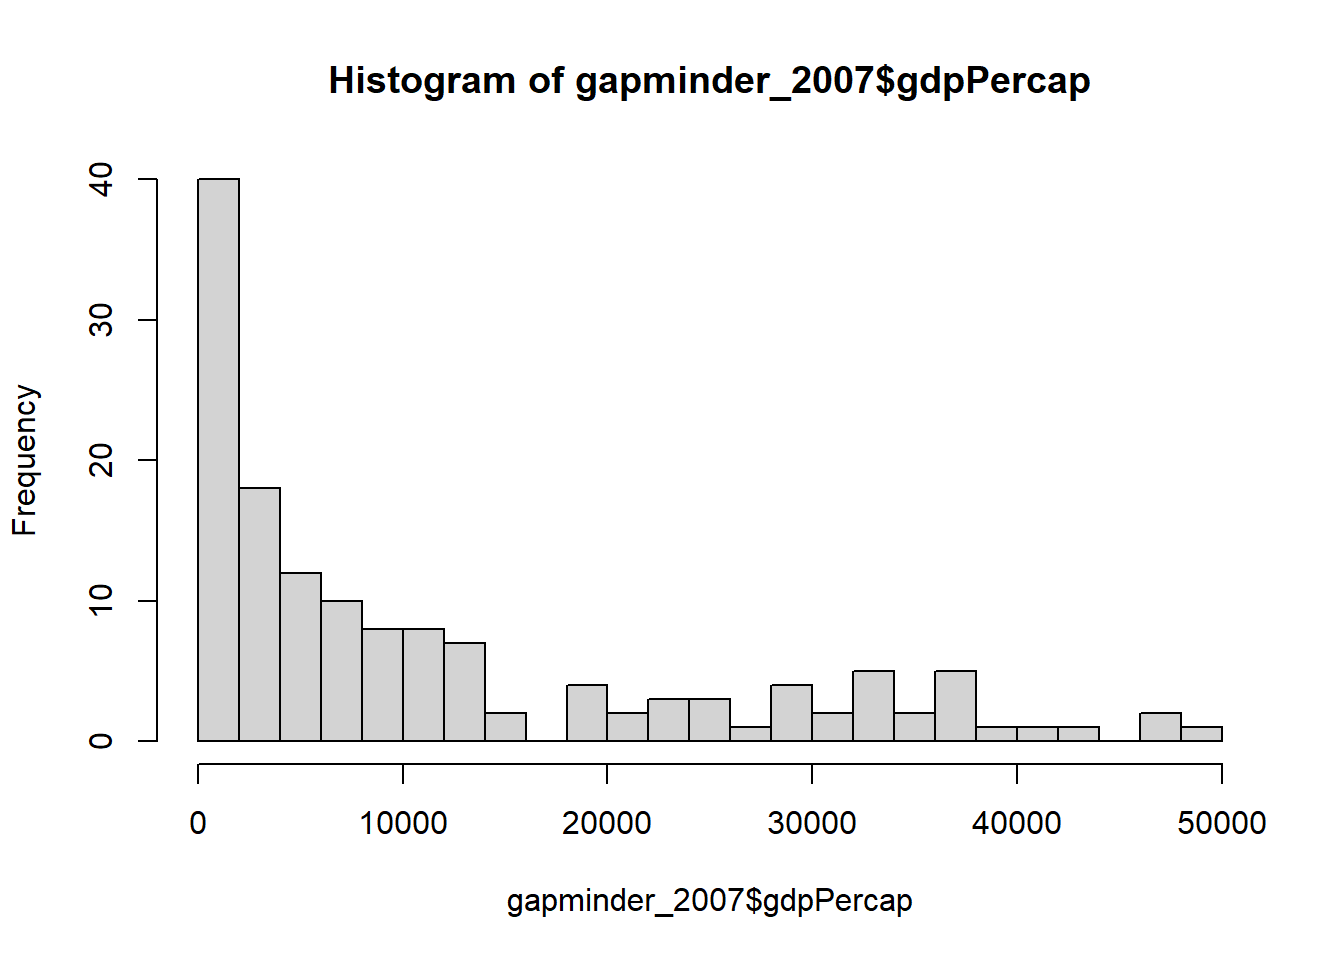
\includegraphics{04-tidyverser_files/figure-latex/unnamed-chunk-90-1.pdf}

\begin{Shaded}
\begin{Highlighting}[]


\CommentTok{\# density plot}
\FunctionTok{plot}\NormalTok{(}\FunctionTok{density}\NormalTok{(gapminder\_2007}\SpecialCharTok{$}\NormalTok{gdpPercap))}
\end{Highlighting}
\end{Shaded}

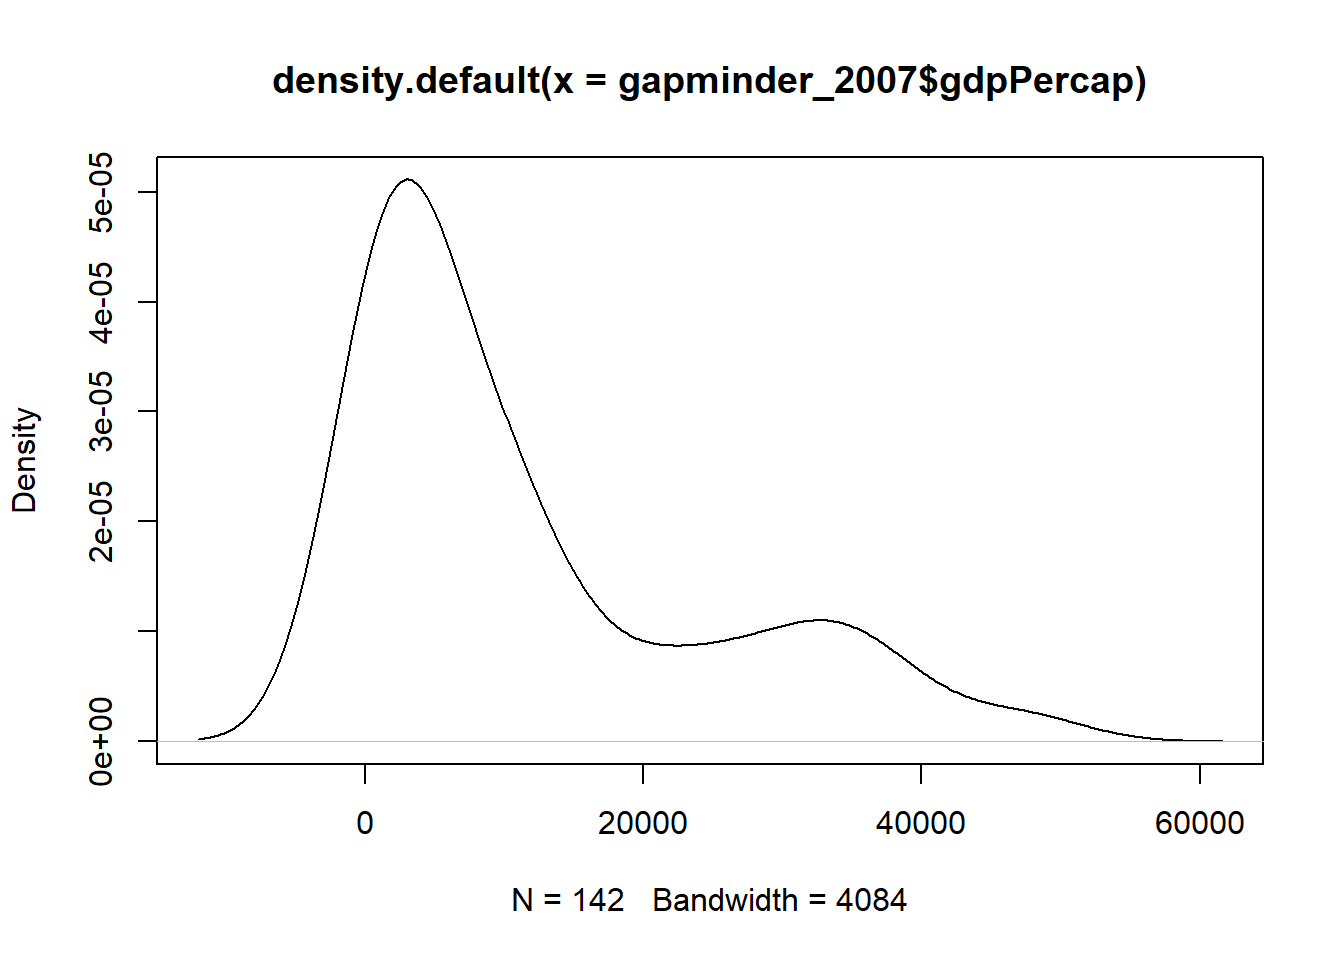
\includegraphics{04-tidyverser_files/figure-latex/unnamed-chunk-90-2.pdf}

\begin{Shaded}
\begin{Highlighting}[]


\CommentTok{\# boxplot of population}
\FunctionTok{boxplot}\NormalTok{(gapminder\_2007}\SpecialCharTok{$}\NormalTok{gdpPercap)}
\end{Highlighting}
\end{Shaded}

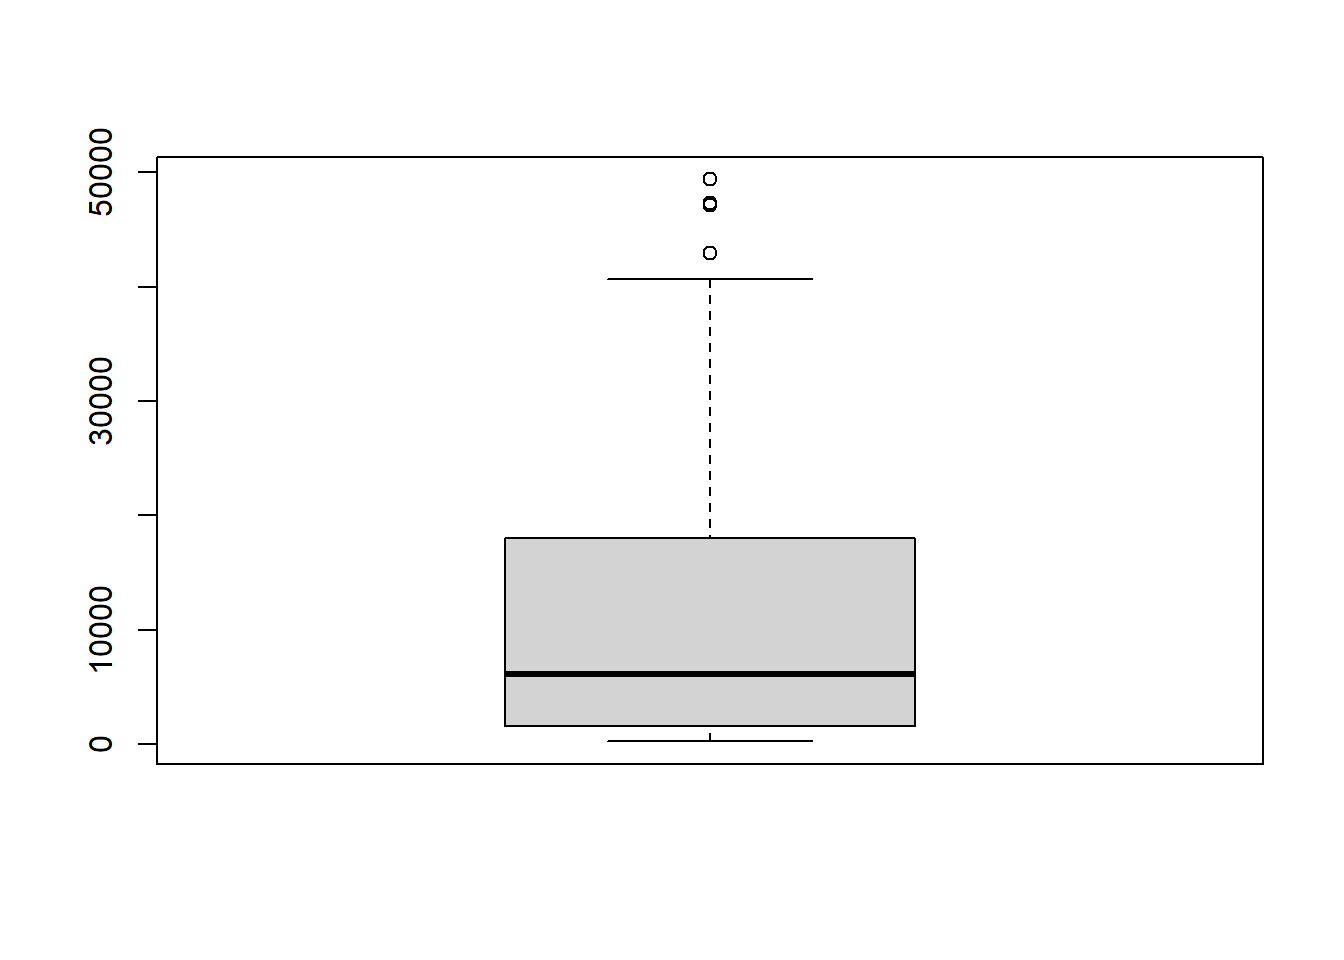
\includegraphics{04-tidyverser_files/figure-latex/unnamed-chunk-90-3.pdf}

Of the above data visualizations, the boxplot is the most relevant as it shows both the spread of data and outliers. The boxplot reveals the following:

\begin{itemize}
\tightlist
\item
  minimum value,
\item
  first quantile (Q1),
\item
  median (second quantile),
\item
  third quantile (Q3),
\item
  maximum value excluding outliers and
\item
  outliers.
\end{itemize}

The difference between Q3 and Q1 is known as the Interquartile Range (IQR).

The outliers within the box plot are calculated as any value that falls beyond 1.5 * IQR.

The function \texttt{boxplot.stats()} computes the data that is used to draw the box plot. Using this function, we can get our outliers.

\begin{Shaded}
\begin{Highlighting}[]
\FunctionTok{boxplot.stats}\NormalTok{(gapminder\_2007}\SpecialCharTok{$}\NormalTok{gdpPercap)}
\CommentTok{\#\textgreater{} $stats}
\CommentTok{\#\textgreater{} [1]   277.5519  1598.4351  6124.3711 18008.9444 40675.9964}
\CommentTok{\#\textgreater{} }
\CommentTok{\#\textgreater{} $n}
\CommentTok{\#\textgreater{} [1] 142}
\CommentTok{\#\textgreater{} }
\CommentTok{\#\textgreater{} $conf}
\CommentTok{\#\textgreater{} [1] 3948.491 8300.251}
\CommentTok{\#\textgreater{} }
\CommentTok{\#\textgreater{} $out}
\CommentTok{\#\textgreater{} [1] 47306.99 49357.19 47143.18 42951.65}
\end{Highlighting}
\end{Shaded}

The first element returned is the summary statistic as was calculated with \texttt{summary()}.

\begin{Shaded}
\begin{Highlighting}[]
\FunctionTok{boxplot.stats}\NormalTok{(gapminder\_2007}\SpecialCharTok{$}\NormalTok{gdpPercap)}\SpecialCharTok{$}\NormalTok{stats}
\CommentTok{\#\textgreater{} [1]   277.5519  1598.4351  6124.3711 18008.9444 40675.9964}
\FunctionTok{summary}\NormalTok{(gapminder\_2007}\SpecialCharTok{$}\NormalTok{gdpPercap)}
\CommentTok{\#\textgreater{}    Min. 1st Qu.  Median    Mean 3rd Qu.    Max. }
\CommentTok{\#\textgreater{}   277.6  1624.8  6124.4 11680.1 18008.8 49357.2}
\end{Highlighting}
\end{Shaded}

The last element returned are the outliers.

\begin{Shaded}
\begin{Highlighting}[]
\FunctionTok{boxplot.stats}\NormalTok{(gapminder\_2007}\SpecialCharTok{$}\NormalTok{gdpPercap)}\SpecialCharTok{$}\NormalTok{out}
\CommentTok{\#\textgreater{} [1] 47306.99 49357.19 47143.18 42951.65}
\end{Highlighting}
\end{Shaded}

Recall outliers are calculated as 1.5 * IQR, this can be changed using the argument coef. By default, it is set to 1.5 but can be changed as need be.

\begin{Shaded}
\begin{Highlighting}[]
\CommentTok{\# changing coef}
\FunctionTok{boxplot.stats}\NormalTok{(gapminder\_2007}\SpecialCharTok{$}\NormalTok{gdpPercap, }\AttributeTok{coef =} \FloatTok{0.8}\NormalTok{)}\SpecialCharTok{$}\NormalTok{out}
\CommentTok{\#\textgreater{}  [1] 34435.37 36126.49 33692.61 36319.24 35278.42 33207.08}
\CommentTok{\#\textgreater{}  [7] 32170.37 39724.98 36180.79 40676.00 31656.07 47306.99}
\CommentTok{\#\textgreater{} [13] 36797.93 49357.19 47143.18 33859.75 37506.42 33203.26}
\CommentTok{\#\textgreater{} [19] 42951.65}
\FunctionTok{boxplot.stats}\NormalTok{(gapminder\_2007}\SpecialCharTok{$}\NormalTok{gdpPercap, }\AttributeTok{coef =} \DecValTok{1}\NormalTok{)}\SpecialCharTok{$}\NormalTok{out}
\CommentTok{\#\textgreater{}  [1] 34435.37 36126.49 36319.24 35278.42 39724.98 36180.79}
\CommentTok{\#\textgreater{}  [7] 40676.00 47306.99 36797.93 49357.19 47143.18 37506.42}
\CommentTok{\#\textgreater{} [13] 42951.65}
\FunctionTok{boxplot.stats}\NormalTok{(gapminder\_2007}\SpecialCharTok{$}\NormalTok{gdpPercap, }\AttributeTok{coef =} \FloatTok{1.2}\NormalTok{)}\SpecialCharTok{$}\NormalTok{out}
\CommentTok{\#\textgreater{} [1] 39724.98 40676.00 47306.99 49357.19 47143.18 42951.65}

\CommentTok{\# selecting outliers}
\FunctionTok{subset}\NormalTok{(gapminder\_2007, gdpPercap }\SpecialCharTok{\textgreater{}=} \FunctionTok{min}\NormalTok{(}\FunctionTok{boxplot.stats}\NormalTok{(gdpPercap)}\SpecialCharTok{$}\NormalTok{out))}
\CommentTok{\#\textgreater{} \# A tibble: 4 x 5}
\CommentTok{\#\textgreater{}   country       continent lifeExp       pop gdpPercap}
\CommentTok{\#\textgreater{}   \textless{}fct\textgreater{}         \textless{}fct\textgreater{}       \textless{}dbl\textgreater{}     \textless{}int\textgreater{}     \textless{}dbl\textgreater{}}
\CommentTok{\#\textgreater{} 1 Kuwait        Asia         77.6   2505559    47307.}
\CommentTok{\#\textgreater{} 2 Norway        Europe       80.2   4627926    49357.}
\CommentTok{\#\textgreater{} 3 Singapore     Asia         80.0   4553009    47143.}
\CommentTok{\#\textgreater{} 4 United States Americas     78.2 301139947    42952.}
\end{Highlighting}
\end{Shaded}

\hypertarget{outliers-by-groups}{%
\subsection{Outliers by groups}\label{outliers-by-groups}}

\begin{Shaded}
\begin{Highlighting}[]
\CommentTok{\# boxplot by continent}
\FunctionTok{boxplot}\NormalTok{(gdpPercap }\SpecialCharTok{\textasciitilde{}}\NormalTok{ continent, gapminder\_2007)}
\end{Highlighting}
\end{Shaded}

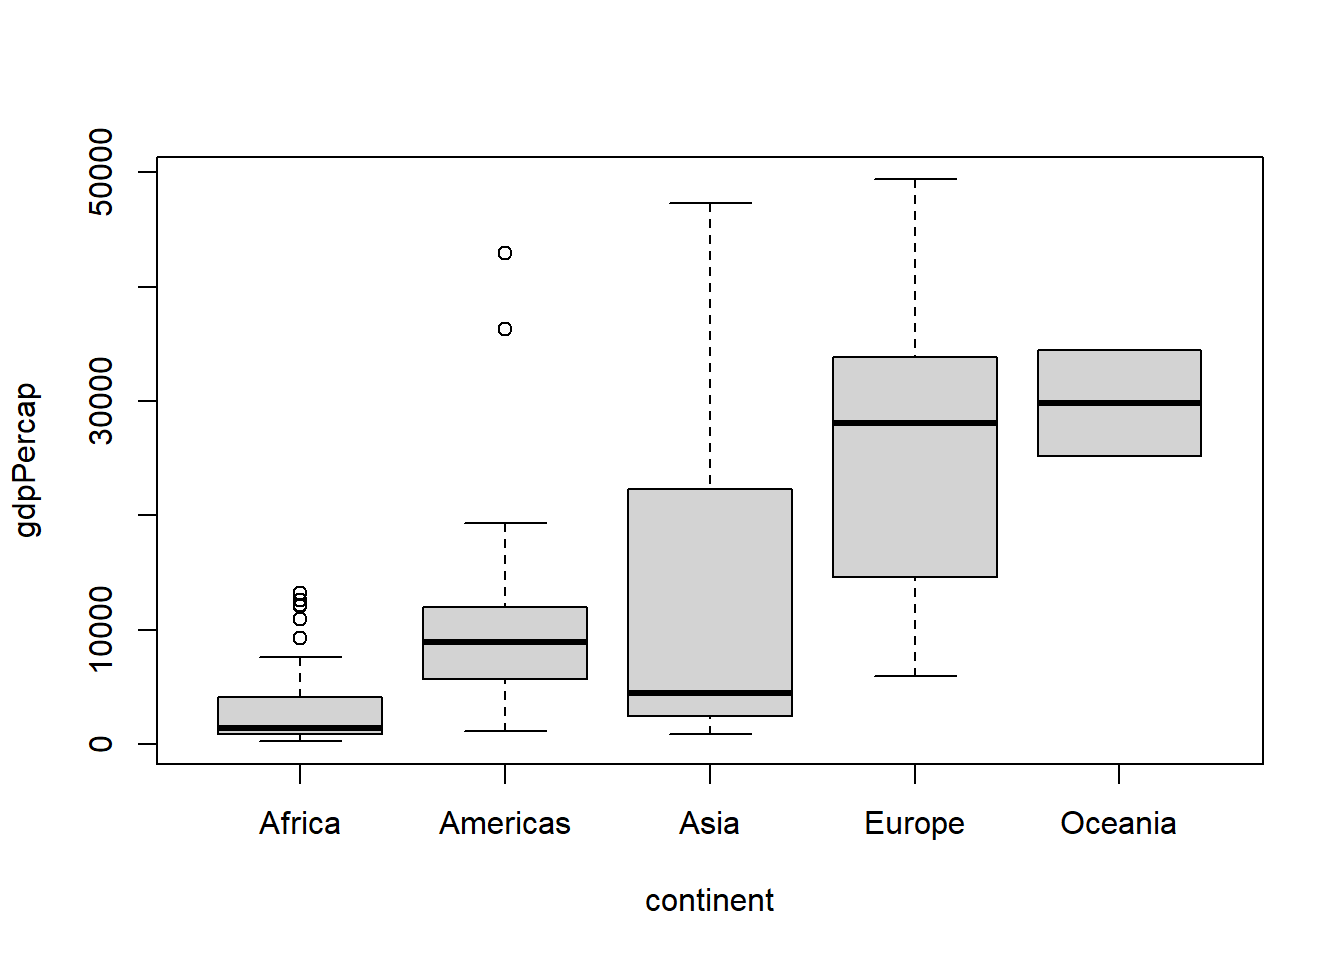
\includegraphics{04-tidyverser_files/figure-latex/unnamed-chunk-95-1.pdf}

\begin{Shaded}
\begin{Highlighting}[]


\CommentTok{\# splitting data frame}
\NormalTok{gap\_split }\OtherTok{\textless{}{-}} \FunctionTok{split}\NormalTok{(gapminder\_2007, gapminder\_2007}\SpecialCharTok{$}\NormalTok{continent)}

\NormalTok{outliers\_2007 }\OtherTok{\textless{}{-}} 
\FunctionTok{lapply}\NormalTok{(gap\_split, }\ControlFlowTok{function}\NormalTok{(x) \{}
\NormalTok{    x }\OtherTok{\textless{}{-}} \FunctionTok{boxplot.stats}\NormalTok{(x}\SpecialCharTok{$}\NormalTok{gdpPercap)}\SpecialCharTok{$}\NormalTok{out}
    \FunctionTok{return}\NormalTok{(x)}
\NormalTok{\})}
\NormalTok{outliers\_2007}
\CommentTok{\#\textgreater{} $Africa}
\CommentTok{\#\textgreater{} [1] 12569.852 12154.090 13206.485 12057.499 10956.991}
\CommentTok{\#\textgreater{} [6]  9269.658}
\CommentTok{\#\textgreater{} }
\CommentTok{\#\textgreater{} $Americas}
\CommentTok{\#\textgreater{} [1] 36319.24 42951.65}
\CommentTok{\#\textgreater{} }
\CommentTok{\#\textgreater{} $Asia}
\CommentTok{\#\textgreater{} numeric(0)}
\CommentTok{\#\textgreater{} }
\CommentTok{\#\textgreater{} $Europe}
\CommentTok{\#\textgreater{} numeric(0)}
\CommentTok{\#\textgreater{} }
\CommentTok{\#\textgreater{} $Oceania}
\CommentTok{\#\textgreater{} numeric(0)}
\end{Highlighting}
\end{Shaded}

\hypertarget{tr-string}{%
\section{String manipulation with stringr}\label{tr-string}}

\hypertarget{determine-string-length}{%
\subsection{Determine string length}\label{determine-string-length}}

The function \texttt{str\_length()} returns the count of letters in a string.

\begin{Shaded}
\begin{Highlighting}[]
\FunctionTok{library}\NormalTok{(stringr)}
\NormalTok{month.name}
\CommentTok{\#\textgreater{}  [1] "January"   "February"  "March"     "April"    }
\CommentTok{\#\textgreater{}  [5] "May"       "June"      "July"      "August"   }
\CommentTok{\#\textgreater{}  [9] "September" "October"   "November"  "December"}
\FunctionTok{str\_length}\NormalTok{(month.name)}
\CommentTok{\#\textgreater{}  [1] 7 8 5 5 3 4 4 6 9 7 8 8}
\end{Highlighting}
\end{Shaded}

\hypertarget{strings-formatting-case-conversion}{%
\subsection{Strings formatting (case conversion)}\label{strings-formatting-case-conversion}}

The functions \texttt{str\_to\_upper()}, \texttt{str\_to\_lower()}, \texttt{str\_to\_title()} and \texttt{str\_to\_sentence()} are used to convert to upper, lower, title and sentence cases respectively.

The function \texttt{str\_pad()} is used to pad characters before and/or after a string.
The function \texttt{str\_trunc()} is used to truncate a string.

\begin{Shaded}
\begin{Highlighting}[]
\CommentTok{\# lowercase}
\FunctionTok{str\_to\_lower}\NormalTok{(}\StringTok{\textquotesingle{}It is an everyday thing\textquotesingle{}}\NormalTok{, }\AttributeTok{locale =} \StringTok{"en"}\NormalTok{)}
\CommentTok{\#\textgreater{} [1] "it is an everyday thing"}

\CommentTok{\# uppercase}
\FunctionTok{str\_to\_upper}\NormalTok{(}\StringTok{\textquotesingle{}It is an everyday thing\textquotesingle{}}\NormalTok{, }\AttributeTok{locale =} \StringTok{"en"}\NormalTok{)}
\CommentTok{\#\textgreater{} [1] "IT IS AN EVERYDAY THING"}

\CommentTok{\# title case}
\FunctionTok{str\_to\_title}\NormalTok{(}\StringTok{\textquotesingle{}It is an everyday thing\textquotesingle{}}\NormalTok{, }\AttributeTok{locale =} \StringTok{"en"}\NormalTok{)}
\CommentTok{\#\textgreater{} [1] "It Is An Everyday Thing"}

\CommentTok{\# sentence case}
\FunctionTok{str\_to\_sentence}\NormalTok{(}\StringTok{\textquotesingle{}iT is aN everyDay thIng\textquotesingle{}}\NormalTok{, }\AttributeTok{locale =} \StringTok{"en"}\NormalTok{)}
\CommentTok{\#\textgreater{} [1] "It is an everyday thing"}

\CommentTok{\# padding string}
\FunctionTok{str\_pad}\NormalTok{(}\FunctionTok{c}\NormalTok{(}\DecValTok{12}\NormalTok{, }\DecValTok{235}\NormalTok{, }\StringTok{\textquotesingle{}abd\textquotesingle{}}\NormalTok{, }\StringTok{\textquotesingle{}ame\textquotesingle{}}\NormalTok{), }\AttributeTok{width =} \DecValTok{5}\NormalTok{, }\AttributeTok{pad =} \StringTok{\textquotesingle{}0\textquotesingle{}}\NormalTok{)}
\CommentTok{\#\textgreater{} [1] "00012" "00235" "00abd" "00ame"}
\FunctionTok{str\_pad}\NormalTok{(}\FunctionTok{c}\NormalTok{(}\DecValTok{12}\NormalTok{, }\DecValTok{235}\NormalTok{, }\StringTok{\textquotesingle{}abd\textquotesingle{}}\NormalTok{, }\StringTok{\textquotesingle{}ame\textquotesingle{}}\NormalTok{), }\AttributeTok{width =} \DecValTok{5}\NormalTok{, }\AttributeTok{pad =} \StringTok{\textquotesingle{}X\textquotesingle{}}\NormalTok{, }\AttributeTok{side =} \StringTok{\textquotesingle{}right\textquotesingle{}}\NormalTok{)}
\CommentTok{\#\textgreater{} [1] "12XXX" "235XX" "abdXX" "ameXX"}
\FunctionTok{str\_pad}\NormalTok{(}\FunctionTok{c}\NormalTok{(}\DecValTok{12}\NormalTok{, }\DecValTok{235}\NormalTok{, }\StringTok{\textquotesingle{}abd\textquotesingle{}}\NormalTok{, }\StringTok{\textquotesingle{}ame\textquotesingle{}}\NormalTok{), }\AttributeTok{width =} \DecValTok{5}\NormalTok{, }\AttributeTok{pad =} \StringTok{\textquotesingle{}{-}\textquotesingle{}}\NormalTok{, }\AttributeTok{side =} \StringTok{\textquotesingle{}both\textquotesingle{}}\NormalTok{)}
\CommentTok{\#\textgreater{} [1] "{-}12{-}{-}" "{-}235{-}" "{-}abd{-}" "{-}ame{-}"}

\CommentTok{\# truncate a character string}
\FunctionTok{str\_trunc}\NormalTok{(state.name[}\DecValTok{1}\SpecialCharTok{:}\DecValTok{8}\NormalTok{], }\AttributeTok{width =} \DecValTok{6}\NormalTok{)}
\CommentTok{\#\textgreater{} [1] "Ala..." "Alaska" "Ari..." "Ark..." "Cal..." "Col..."}
\CommentTok{\#\textgreater{} [7] "Con..." "Del..."}
\FunctionTok{str\_trunc}\NormalTok{(state.name[}\DecValTok{1}\SpecialCharTok{:}\DecValTok{8}\NormalTok{], }\DecValTok{6}\NormalTok{, }\AttributeTok{side  =} \StringTok{\textquotesingle{}left\textquotesingle{}}\NormalTok{)}
\CommentTok{\#\textgreater{} [1] "...ama" "Alaska" "...ona" "...sas" "...nia" "...ado"}
\CommentTok{\#\textgreater{} [7] "...cut" "...are"}
\FunctionTok{str\_trunc}\NormalTok{(state.name[}\DecValTok{1}\SpecialCharTok{:}\DecValTok{8}\NormalTok{], }\DecValTok{6}\NormalTok{, }\AttributeTok{side  =} \StringTok{\textquotesingle{}right\textquotesingle{}}\NormalTok{, }\AttributeTok{ellipsis =} \StringTok{\textquotesingle{}\textquotesingle{}}\NormalTok{)}
\CommentTok{\#\textgreater{} [1] "Alabam" "Alaska" "Arizon" "Arkans" "Califo" "Colora"}
\CommentTok{\#\textgreater{} [7] "Connec" "Delawa"}
\end{Highlighting}
\end{Shaded}

\hypertarget{join-and-split-strings-1}{%
\subsection{Join and Split strings}\label{join-and-split-strings-1}}

\hypertarget{joining-strings-with-str_c}{%
\subsubsection{joining strings with str\_c()}\label{joining-strings-with-str_c}}

The function \texttt{str\_c()} joins two or more vectors element wise into a single character vector, optionally inserting separator (sep) between input vectors.

\begin{Shaded}
\begin{Highlighting}[]
\CommentTok{\# combining elements into a character vector}
\FunctionTok{str\_c}\NormalTok{(}\StringTok{\textquotesingle{}a\textquotesingle{}}\NormalTok{, }\StringTok{\textquotesingle{}b\textquotesingle{}}\NormalTok{)}
\CommentTok{\#\textgreater{} [1] "ab"}
\FunctionTok{str\_c}\NormalTok{(}\DecValTok{1}\NormalTok{, }\DecValTok{2}\NormalTok{, }\DecValTok{3}\NormalTok{, }\DecValTok{4}\NormalTok{)}
\CommentTok{\#\textgreater{} [1] "1234"}

\CommentTok{\# using sep}
\FunctionTok{str\_c}\NormalTok{(}\StringTok{\textquotesingle{}a\textquotesingle{}}\NormalTok{, }\StringTok{\textquotesingle{}b\textquotesingle{}}\NormalTok{, }\AttributeTok{sep =} \StringTok{\textquotesingle{} \textquotesingle{}}\NormalTok{)}
\CommentTok{\#\textgreater{} [1] "a b"}
\FunctionTok{str\_c}\NormalTok{(}\DecValTok{1}\NormalTok{, }\DecValTok{2}\NormalTok{, }\DecValTok{3}\NormalTok{, }\DecValTok{4}\NormalTok{, }\AttributeTok{sep =} \StringTok{\textquotesingle{} \textquotesingle{}}\NormalTok{)}
\CommentTok{\#\textgreater{} [1] "1 2 3 4"}
\FunctionTok{str\_c}\NormalTok{(}\DecValTok{1}\SpecialCharTok{:}\DecValTok{10}\NormalTok{, }\AttributeTok{sep =} \StringTok{\textquotesingle{} \textquotesingle{}}\NormalTok{)}
\CommentTok{\#\textgreater{}  [1] "1"  "2"  "3"  "4"  "5"  "6"  "7"  "8"  "9"  "10"}

\CommentTok{\# on a single vector}
\FunctionTok{str\_c}\NormalTok{(}\FunctionTok{c}\NormalTok{(}\StringTok{\textquotesingle{}a\textquotesingle{}}\NormalTok{, }\StringTok{\textquotesingle{}b\textquotesingle{}}\NormalTok{), }\AttributeTok{sep =} \StringTok{\textquotesingle{} \textless{}\textgreater{} \textquotesingle{}}\NormalTok{)}
\CommentTok{\#\textgreater{} [1] "a" "b"}
\FunctionTok{str\_c}\NormalTok{(}\FunctionTok{c}\NormalTok{(}\DecValTok{1}\NormalTok{, }\DecValTok{2}\NormalTok{), }\AttributeTok{sep =} \StringTok{\textquotesingle{} \textless{}\textgreater{} \textquotesingle{}}\NormalTok{)}
\CommentTok{\#\textgreater{} [1] "1" "2"}

\CommentTok{\# two or more vectors}
\FunctionTok{str\_c}\NormalTok{(}\FunctionTok{c}\NormalTok{(}\StringTok{\textquotesingle{}a\textquotesingle{}}\NormalTok{, }\StringTok{\textquotesingle{}b\textquotesingle{}}\NormalTok{), }\FunctionTok{c}\NormalTok{(}\StringTok{\textquotesingle{}c\textquotesingle{}}\NormalTok{, }\StringTok{\textquotesingle{}d\textquotesingle{}}\NormalTok{), }\AttributeTok{sep =} \StringTok{\textquotesingle{} \textless{}\textgreater{} \textquotesingle{}}\NormalTok{)}
\CommentTok{\#\textgreater{} [1] "a \textless{}\textgreater{} c" "b \textless{}\textgreater{} d"}
\FunctionTok{str\_c}\NormalTok{(}\DecValTok{1}\SpecialCharTok{:}\DecValTok{5}\NormalTok{, }\DecValTok{10}\SpecialCharTok{:}\DecValTok{20}\NormalTok{, }\AttributeTok{sep =} \StringTok{\textquotesingle{} \textquotesingle{}}\NormalTok{)}
\CommentTok{\#\textgreater{}  [1] "1 10" "2 11" "3 12" "4 13" "5 14" "1 15" "2 16" "3 17"}
\CommentTok{\#\textgreater{}  [9] "4 18" "5 19" "1 20"}
\FunctionTok{str\_c}\NormalTok{(}\DecValTok{1}\SpecialCharTok{:}\DecValTok{5}\NormalTok{, }\DecValTok{10}\SpecialCharTok{:}\DecValTok{20}\NormalTok{, }\FunctionTok{c}\NormalTok{(}\StringTok{\textquotesingle{}a\textquotesingle{}}\NormalTok{,}\StringTok{\textquotesingle{}b\textquotesingle{}}\NormalTok{,}\StringTok{\textquotesingle{}c\textquotesingle{}}\NormalTok{), }\AttributeTok{sep =} \StringTok{\textquotesingle{} \textquotesingle{}}\NormalTok{)}
\CommentTok{\#\textgreater{}  [1] "1 10 a" "2 11 b" "3 12 c" "4 13 a" "5 14 b" "1 15 c"}
\CommentTok{\#\textgreater{}  [7] "2 16 a" "3 17 b" "4 18 c" "5 19 a" "1 20 b"}
\CommentTok{\# collapsing vectors}
\FunctionTok{str\_c}\NormalTok{(}\DecValTok{1}\SpecialCharTok{:}\DecValTok{10}\NormalTok{, }\AttributeTok{collapse =} \StringTok{\textquotesingle{}\textasciitilde{}\textquotesingle{}}\NormalTok{)}
\CommentTok{\#\textgreater{} [1] "1\textasciitilde{}2\textasciitilde{}3\textasciitilde{}4\textasciitilde{}5\textasciitilde{}6\textasciitilde{}7\textasciitilde{}8\textasciitilde{}9\textasciitilde{}10"}
\FunctionTok{str\_c}\NormalTok{(}\FunctionTok{c}\NormalTok{(}\StringTok{\textquotesingle{}a\textquotesingle{}}\NormalTok{, }\StringTok{\textquotesingle{}b\textquotesingle{}}\NormalTok{), }\FunctionTok{c}\NormalTok{(}\StringTok{\textquotesingle{}c\textquotesingle{}}\NormalTok{, }\StringTok{\textquotesingle{}d\textquotesingle{}}\NormalTok{), }\AttributeTok{collapse =} \StringTok{\textquotesingle{} \textless{}\textgreater{} \textquotesingle{}}\NormalTok{)}
\CommentTok{\#\textgreater{} [1] "ac \textless{}\textgreater{} bd"}
\FunctionTok{str\_c}\NormalTok{(month.name[}\DecValTok{1}\SpecialCharTok{:}\DecValTok{6}\NormalTok{], }\AttributeTok{collapse =} \StringTok{" {-} "}\NormalTok{)}
\CommentTok{\#\textgreater{} [1] "January {-} February {-} March {-} April {-} May {-} June"}

\NormalTok{a }\OtherTok{\textless{}{-}}\NormalTok{ month.name[}\DecValTok{1}\NormalTok{]}
\NormalTok{b }\OtherTok{\textless{}{-}}\NormalTok{ month.name[}\DecValTok{2}\NormalTok{]}
\NormalTok{c }\OtherTok{\textless{}{-}}\NormalTok{ month.name[}\DecValTok{3}\NormalTok{]}

\CommentTok{\# combining character and variables}
\FunctionTok{str\_c}\NormalTok{(b,}\StringTok{\textquotesingle{}comes after\textquotesingle{}}\NormalTok{, a ,}\StringTok{\textquotesingle{}but comes before\textquotesingle{}}\NormalTok{, c, }\AttributeTok{sep =} \StringTok{" "}\NormalTok{)}
\CommentTok{\#\textgreater{} [1] "February comes after January but comes before March"}
\FunctionTok{str\_c}\NormalTok{(b,}\StringTok{\textquotesingle{}comes after\textquotesingle{}}\NormalTok{, a ,}\StringTok{\textquotesingle{}but comes before\textquotesingle{}}\NormalTok{, c, }\AttributeTok{sep =} \StringTok{"/"}\NormalTok{)}
\CommentTok{\#\textgreater{} [1] "February/comes after/January/but comes before/March"}
\FunctionTok{str\_c}\NormalTok{(}\StringTok{\textquotesingle{}version 1.\textquotesingle{}}\NormalTok{, }\DecValTok{1}\SpecialCharTok{:}\DecValTok{5}\NormalTok{, }\AttributeTok{sep =} \StringTok{\textquotesingle{}\textquotesingle{}}\NormalTok{)}
\CommentTok{\#\textgreater{} [1] "version 1.1" "version 1.2" "version 1.3" "version 1.4"}
\CommentTok{\#\textgreater{} [5] "version 1.5"}
\end{Highlighting}
\end{Shaded}

\hypertarget{joining-using-str_glue}{%
\subsection{Joining using str\_glue()}\label{joining-using-str_glue}}

The function \texttt{str\_glue()} returns a character vector containing a formatted combination of text and variable values.

\textbf{formatting with integers}

\begin{Shaded}
\begin{Highlighting}[]
\NormalTok{x }\OtherTok{\textless{}{-}} \DecValTok{2}
\FunctionTok{str\_glue}\NormalTok{(}\StringTok{\textquotesingle{}\{x\} * \{x\} = \{x ** 2\}\textquotesingle{}}\NormalTok{)}
\CommentTok{\#\textgreater{} 2 * 2 = 4}

\NormalTok{x }\OtherTok{\textless{}{-}} \FunctionTok{c}\NormalTok{(}\DecValTok{1}\SpecialCharTok{:}\DecValTok{4}\NormalTok{)}
\FunctionTok{str\_glue}\NormalTok{(}\StringTok{\textquotesingle{}\{x\} squared is equal to \{x ** 2\}\textquotesingle{}}\NormalTok{)}
\CommentTok{\#\textgreater{} 1 squared is equal to 1}
\CommentTok{\#\textgreater{} 2 squared is equal to 4}
\CommentTok{\#\textgreater{} 3 squared is equal to 9}
\CommentTok{\#\textgreater{} 4 squared is equal to 16}

\NormalTok{num }\OtherTok{\textless{}{-}} \FunctionTok{c}\NormalTok{(}\DecValTok{123}\NormalTok{, }\DecValTok{1}\NormalTok{, }\DecValTok{100}\NormalTok{, }\DecValTok{200}\NormalTok{, }\DecValTok{10200}\NormalTok{, }\DecValTok{25000}\NormalTok{)}
\FunctionTok{str\_glue}\NormalTok{(}\StringTok{\textquotesingle{}my registration number is \{str\_pad(num, 5, pad = "0")\}\textquotesingle{}}\NormalTok{)}
\CommentTok{\#\textgreater{} my registration number is 00123}
\CommentTok{\#\textgreater{} my registration number is 00001}
\CommentTok{\#\textgreater{} my registration number is 00100}
\CommentTok{\#\textgreater{} my registration number is 00200}
\CommentTok{\#\textgreater{} my registration number is 10200}
\CommentTok{\#\textgreater{} my registration number is 25000}
\end{Highlighting}
\end{Shaded}

\textbf{Formatting with strings}

\begin{Shaded}
\begin{Highlighting}[]
\NormalTok{x }\OtherTok{\textless{}{-}} \StringTok{\textquotesingle{}my name is\textquotesingle{}}
\NormalTok{y }\OtherTok{\textless{}{-}} \StringTok{\textquotesingle{}james\textquotesingle{}}
\NormalTok{z }\OtherTok{\textless{}{-}} \StringTok{\textquotesingle{}london\textquotesingle{}}
\FunctionTok{str\_glue}\NormalTok{(}\StringTok{\textquotesingle{}\{x\} \{y\} and i live and work in \{z\}\textquotesingle{}}\NormalTok{)}
\CommentTok{\#\textgreater{} my name is james and i live and work in london}


\NormalTok{x }\OtherTok{\textless{}{-}} \StringTok{\textquotesingle{}my name is\textquotesingle{}}
\NormalTok{y }\OtherTok{\textless{}{-}} \StringTok{\textquotesingle{}james\textquotesingle{}}
\NormalTok{z }\OtherTok{\textless{}{-}} \DecValTok{35}
\FunctionTok{str\_glue}\NormalTok{(}\StringTok{\textquotesingle{}\{str\_to\_title(x)\} \{str\_to\_upper(y)\} and i am \{z\} years\textquotesingle{}}\NormalTok{)}
\CommentTok{\#\textgreater{} My Name Is JAMES and i am 35 years}

\NormalTok{names }\OtherTok{\textless{}{-}} \FunctionTok{c}\NormalTok{(}\StringTok{\textquotesingle{}paul\textquotesingle{}}\NormalTok{, }\StringTok{\textquotesingle{}alphonse\textquotesingle{}}\NormalTok{, }\StringTok{\textquotesingle{}michael\textquotesingle{}}\NormalTok{, }\StringTok{\textquotesingle{}james\textquotesingle{}}\NormalTok{, }\StringTok{\textquotesingle{}samson\textquotesingle{}}\NormalTok{, }\StringTok{\textquotesingle{}terence\textquotesingle{}}\NormalTok{, }\StringTok{\textquotesingle{}derin\textquotesingle{}}\NormalTok{)}
\NormalTok{age }\OtherTok{\textless{}{-}} \FunctionTok{c}\NormalTok{(}\DecValTok{30}\NormalTok{, }\DecValTok{35}\NormalTok{, }\DecValTok{32}\NormalTok{, }\DecValTok{37}\NormalTok{, }\DecValTok{29}\NormalTok{, }\DecValTok{40}\NormalTok{, }\DecValTok{30}\NormalTok{)}
\FunctionTok{str\_glue}\NormalTok{(}\StringTok{\textquotesingle{}i am \{str\_to\_title(names)\} and i am \{age\} years old\textquotesingle{}}\NormalTok{)}
\CommentTok{\#\textgreater{} i am Paul and i am 30 years old}
\CommentTok{\#\textgreater{} i am Alphonse and i am 35 years old}
\CommentTok{\#\textgreater{} i am Michael and i am 32 years old}
\CommentTok{\#\textgreater{} i am James and i am 37 years old}
\CommentTok{\#\textgreater{} i am Samson and i am 29 years old}
\CommentTok{\#\textgreater{} i am Terence and i am 40 years old}
\CommentTok{\#\textgreater{} i am Derin and i am 30 years old}
\end{Highlighting}
\end{Shaded}

\textbf{Formatting with doubles or floating points}

\begin{Shaded}
\begin{Highlighting}[]
\NormalTok{x }\OtherTok{\textless{}{-}} \DecValTok{1000}\SpecialCharTok{/}\DecValTok{6}
\NormalTok{x}
\CommentTok{\#\textgreater{} [1] 166.6667}
\FunctionTok{str\_glue}\NormalTok{(}\StringTok{\textquotesingle{}1000 divided by 3 is \{x\}\textquotesingle{}}\NormalTok{)}
\CommentTok{\#\textgreater{} 1000 divided by 3 is 166.666666666667}
\FunctionTok{str\_glue}\NormalTok{(}\StringTok{\textquotesingle{}1000 divided by 3 is \{round(x, 3)\}\textquotesingle{}}\NormalTok{)}
\CommentTok{\#\textgreater{} 1000 divided by 3 is 166.667}
\FunctionTok{str\_glue}\NormalTok{(}\StringTok{\textquotesingle{}1000 divided by 3 is \{round(x)\}\textquotesingle{}}\NormalTok{)}
\CommentTok{\#\textgreater{} 1000 divided by 3 is 167}
\FunctionTok{str\_glue}\NormalTok{(}\StringTok{\textquotesingle{}1000 divided by 3 is \{paste0("+", round(x))\}\textquotesingle{}}\NormalTok{)}
\CommentTok{\#\textgreater{} 1000 divided by 3 is +167}
\FunctionTok{str\_glue}\NormalTok{(}\StringTok{\textquotesingle{}1000 divided by 3 is\{paste0(" ", round(x))\}\textquotesingle{}}\NormalTok{)}
\CommentTok{\#\textgreater{} 1000 divided by 3 is 167}
\end{Highlighting}
\end{Shaded}

\hypertarget{splitting-strings-using-str_split-and-str_split_fixed}{%
\subsection{Splitting strings using str\_split() and str\_split\_fixed()}\label{splitting-strings-using-str_split-and-str_split_fixed}}

The function \texttt{str\_split()} splits the elements of a character vector into substrings by a specific pattern.
The function \texttt{str\_split\_fixed()} splits up the elements of a character into a fixed number of pieces.

\begin{Shaded}
\begin{Highlighting}[]
\FunctionTok{str}\NormalTok{(}\FunctionTok{str\_split}\NormalTok{(}\FunctionTok{c}\NormalTok{(}\StringTok{\textquotesingle{}2020{-}01{-}01\textquotesingle{}}\NormalTok{, }\StringTok{\textquotesingle{}2019{-}03{-}31\textquotesingle{}}\NormalTok{, }\StringTok{\textquotesingle{}2018{-}06{-}30\textquotesingle{}}\NormalTok{), }\AttributeTok{pattern =} \StringTok{"{-}"}\NormalTok{))}
\CommentTok{\#\textgreater{} List of 3}
\CommentTok{\#\textgreater{}  $ : chr [1:3] "2020" "01" "01"}
\CommentTok{\#\textgreater{}  $ : chr [1:3] "2019" "03" "31"}
\CommentTok{\#\textgreater{}  $ : chr [1:3] "2018" "06" "30"}
\FunctionTok{str}\NormalTok{(}\FunctionTok{str\_split}\NormalTok{(}\FunctionTok{c}\NormalTok{(}\StringTok{\textquotesingle{}2020 01 01\textquotesingle{}}\NormalTok{, }\StringTok{\textquotesingle{}2019 03 31\textquotesingle{}}\NormalTok{, }\StringTok{\textquotesingle{}2018 06 30\textquotesingle{}}\NormalTok{), }\AttributeTok{pattern =} \StringTok{" "}\NormalTok{))}
\CommentTok{\#\textgreater{} List of 3}
\CommentTok{\#\textgreater{}  $ : chr [1:3] "2020" "01" "01"}
\CommentTok{\#\textgreater{}  $ : chr [1:3] "2019" "03" "31"}
\CommentTok{\#\textgreater{}  $ : chr [1:3] "2018" "06" "30"}

\CommentTok{\# splitting into two substrings}
\FunctionTok{str}\NormalTok{(}\FunctionTok{str\_split}\NormalTok{(}\FunctionTok{c}\NormalTok{(}\StringTok{\textquotesingle{}2020{-}01{-}01\textquotesingle{}}\NormalTok{, }\StringTok{\textquotesingle{}2019{-}03{-}31\textquotesingle{}}\NormalTok{, }\StringTok{\textquotesingle{}2018{-}06{-}30\textquotesingle{}}\NormalTok{), }\AttributeTok{pattern =} \StringTok{"{-}"}\NormalTok{, }\AttributeTok{n =} \DecValTok{2}\NormalTok{))}
\CommentTok{\#\textgreater{} List of 3}
\CommentTok{\#\textgreater{}  $ : chr [1:2] "2020" "01{-}01"}
\CommentTok{\#\textgreater{}  $ : chr [1:2] "2019" "03{-}31"}
\CommentTok{\#\textgreater{}  $ : chr [1:2] "2018" "06{-}30"}
\FunctionTok{str}\NormalTok{(}\FunctionTok{str\_split}\NormalTok{(}\FunctionTok{c}\NormalTok{(}\StringTok{\textquotesingle{}2020 01 01\textquotesingle{}}\NormalTok{, }\StringTok{\textquotesingle{}2019 03 31\textquotesingle{}}\NormalTok{, }\StringTok{\textquotesingle{}2018 06 30\textquotesingle{}}\NormalTok{), }\AttributeTok{pattern =} \StringTok{" "}\NormalTok{, }\AttributeTok{n =} \DecValTok{2}\NormalTok{))}
\CommentTok{\#\textgreater{} List of 3}
\CommentTok{\#\textgreater{}  $ : chr [1:2] "2020" "01 01"}
\CommentTok{\#\textgreater{}  $ : chr [1:2] "2019" "03 31"}
\CommentTok{\#\textgreater{}  $ : chr [1:2] "2018" "06 30"}

\CommentTok{\# returning a matrix}
\FunctionTok{str\_split\_fixed}\NormalTok{(}\FunctionTok{c}\NormalTok{(}\StringTok{\textquotesingle{}2020{-}01{-}01\textquotesingle{}}\NormalTok{, }\StringTok{\textquotesingle{}2019{-}03{-}31\textquotesingle{}}\NormalTok{, }\StringTok{\textquotesingle{}2018{-}06{-}30\textquotesingle{}}\NormalTok{), }\StringTok{\textquotesingle{}{-}\textquotesingle{}}\NormalTok{, }\DecValTok{2}\NormalTok{)}
\CommentTok{\#\textgreater{}      [,1]   [,2]   }
\CommentTok{\#\textgreater{} [1,] "2020" "01{-}01"}
\CommentTok{\#\textgreater{} [2,] "2019" "03{-}31"}
\CommentTok{\#\textgreater{} [3,] "2018" "06{-}30"}
\FunctionTok{str\_split\_fixed}\NormalTok{(}\FunctionTok{c}\NormalTok{(}\StringTok{\textquotesingle{}2020{-}01{-}01\textquotesingle{}}\NormalTok{, }\StringTok{\textquotesingle{}2019{-}03{-}31\textquotesingle{}}\NormalTok{, }\StringTok{\textquotesingle{}2018{-}06{-}30\textquotesingle{}}\NormalTok{), }\StringTok{\textquotesingle{}{-}\textquotesingle{}}\NormalTok{, }\DecValTok{3}\NormalTok{)}
\CommentTok{\#\textgreater{}      [,1]   [,2] [,3]}
\CommentTok{\#\textgreater{} [1,] "2020" "01" "01"}
\CommentTok{\#\textgreater{} [2,] "2019" "03" "31"}
\CommentTok{\#\textgreater{} [3,] "2018" "06" "30"}
\end{Highlighting}
\end{Shaded}

\hypertarget{extract-and-replace-part-of-a-string}{%
\subsection{Extract and Replace part of a string}\label{extract-and-replace-part-of-a-string}}

\hypertarget{extracting-string-values-using-str_sub}{%
\subsubsection{Extracting string values using str\_sub()}\label{extracting-string-values-using-str_sub}}

The function \texttt{str\_sub()} extracts a substring from a string by indexing. It uses start for the beginning position and stop for the ending position. It is like indexing but applied to a string.

\begin{Shaded}
\begin{Highlighting}[]
\NormalTok{var }\OtherTok{\textless{}{-}} \FunctionTok{c}\NormalTok{(}\StringTok{\textquotesingle{}2020{-}01{-}01\textquotesingle{}}\NormalTok{, }\StringTok{\textquotesingle{}2019{-}03{-}31\textquotesingle{}}\NormalTok{, }\StringTok{\textquotesingle{}2018{-}06{-}30\textquotesingle{}}\NormalTok{)}
\FunctionTok{str\_sub}\NormalTok{(var, }\AttributeTok{start =} \DecValTok{1}\NormalTok{, }\AttributeTok{end =} \DecValTok{4}\NormalTok{)}
\CommentTok{\#\textgreater{} [1] "2020" "2019" "2018"}
\FunctionTok{str\_sub}\NormalTok{(var, }\DecValTok{6}\NormalTok{, }\DecValTok{7}\NormalTok{)}
\CommentTok{\#\textgreater{} [1] "01" "03" "06"}
\FunctionTok{str\_sub}\NormalTok{(var, }\DecValTok{9}\NormalTok{, }\DecValTok{10}\NormalTok{)}
\CommentTok{\#\textgreater{} [1] "01" "31" "30"}

\CommentTok{\# using negative numbers}
\FunctionTok{str\_sub}\NormalTok{(var, }\SpecialCharTok{{-}}\DecValTok{2}\NormalTok{, }\SpecialCharTok{{-}}\DecValTok{1}\NormalTok{)}
\CommentTok{\#\textgreater{} [1] "01" "31" "30"}
\FunctionTok{str\_sub}\NormalTok{(var, }\SpecialCharTok{{-}}\DecValTok{5}\NormalTok{, }\SpecialCharTok{{-}}\DecValTok{4}\NormalTok{)}
\CommentTok{\#\textgreater{} [1] "01" "03" "06"}
\FunctionTok{str\_sub}\NormalTok{(var, }\SpecialCharTok{{-}}\DecValTok{10}\NormalTok{, }\SpecialCharTok{{-}}\DecValTok{7}\NormalTok{)}
\CommentTok{\#\textgreater{} [1] "2020" "2019" "2018"}
\end{Highlighting}
\end{Shaded}

\hypertarget{replacing-string-values-using-str_sub}{%
\subsubsection{Replacing string values using str\_sub()}\label{replacing-string-values-using-str_sub}}

The function \texttt{str\_sub()} is also used to replace substring in a string by assigning a different string to the extracted substring.

\begin{Shaded}
\begin{Highlighting}[]
\NormalTok{var }\OtherTok{\textless{}{-}} \FunctionTok{c}\NormalTok{(}\StringTok{\textquotesingle{}2020{-}01{-}01\textquotesingle{}}\NormalTok{, }\StringTok{\textquotesingle{}2019{-}03{-}31\textquotesingle{}}\NormalTok{, }\StringTok{\textquotesingle{}2018{-}06{-}30\textquotesingle{}}\NormalTok{)}
\FunctionTok{str\_sub}\NormalTok{(var, }\DecValTok{1}\NormalTok{, }\DecValTok{4}\NormalTok{) }\OtherTok{\textless{}{-}} \FunctionTok{c}\NormalTok{(}\StringTok{\textquotesingle{}2010\textquotesingle{}}\NormalTok{, }\StringTok{\textquotesingle{}2011\textquotesingle{}}\NormalTok{, }\StringTok{\textquotesingle{}2012\textquotesingle{}}\NormalTok{)}
\NormalTok{var}
\CommentTok{\#\textgreater{} [1] "2010{-}01{-}01" "2011{-}03{-}31" "2012{-}06{-}30"}
\end{Highlighting}
\end{Shaded}

\hypertarget{replacing-string-values-using-str_replace}{%
\subsection{Replacing string values using str\_replace()}\label{replacing-string-values-using-str_replace}}

The function \texttt{str\_replace()} replaces a substring at first occurrence.

\begin{Shaded}
\begin{Highlighting}[]
\NormalTok{var }\OtherTok{\textless{}{-}} \FunctionTok{c}\NormalTok{(}\StringTok{\textquotesingle{}2020{-}01{-}01\textquotesingle{}}\NormalTok{, }\StringTok{\textquotesingle{}2019{-}03{-}31\textquotesingle{}}\NormalTok{, }\StringTok{\textquotesingle{}2018{-}06{-}30\textquotesingle{}}\NormalTok{)}
\FunctionTok{str\_replace}\NormalTok{(var, }\StringTok{"{-}"}\NormalTok{, }\StringTok{""}\NormalTok{)}
\CommentTok{\#\textgreater{} [1] "202001{-}01" "201903{-}31" "201806{-}30"}
\FunctionTok{str\_replace}\NormalTok{(var, }\StringTok{"{-}"}\NormalTok{, }\StringTok{"/"}\NormalTok{)}
\CommentTok{\#\textgreater{} [1] "2020/01{-}01" "2019/03{-}31" "2018/06{-}30"}
\end{Highlighting}
\end{Shaded}

\hypertarget{replacing-string-values-using-str_replace_all}{%
\subsection{Replacing string values using str\_replace\_all()}\label{replacing-string-values-using-str_replace_all}}

The function \texttt{str\_replace\_all()} replaces a substring throughout a string.

\begin{Shaded}
\begin{Highlighting}[]
\NormalTok{var }\OtherTok{\textless{}{-}} \FunctionTok{c}\NormalTok{(}\StringTok{\textquotesingle{}2020{-}01{-}01\textquotesingle{}}\NormalTok{, }\StringTok{\textquotesingle{}2019{-}03{-}31\textquotesingle{}}\NormalTok{, }\StringTok{\textquotesingle{}2018{-}06{-}30\textquotesingle{}}\NormalTok{)}
\FunctionTok{str\_replace\_all}\NormalTok{(var, }\StringTok{"{-}"}\NormalTok{, }\StringTok{" "}\NormalTok{)}
\CommentTok{\#\textgreater{} [1] "2020 01 01" "2019 03 31" "2018 06 30"}
\FunctionTok{str\_replace\_all}\NormalTok{(var, }\StringTok{"{-}"}\NormalTok{, }\StringTok{"/"}\NormalTok{)}
\CommentTok{\#\textgreater{} [1] "2020/01/01" "2019/03/31" "2018/06/30"}
\end{Highlighting}
\end{Shaded}

\hypertarget{remove-white-spaces-and-clean-string-values-1}{%
\subsubsection{Remove white spaces and clean string values}\label{remove-white-spaces-and-clean-string-values-1}}

The function:

\begin{itemize}
\tightlist
\item
  \texttt{str\_trim()} removes white spaces.
\item
  \texttt{str\_squish()} removes repeated spaces.
\item
  \texttt{str\_remove()} removes the first repeated spaces.
\item
  \texttt{str\_remove\_all()} removes all repeated spaces.
\end{itemize}

\begin{Shaded}
\begin{Highlighting}[]
\CommentTok{\# both sides}
\FunctionTok{str\_trim}\NormalTok{(}\FunctionTok{c}\NormalTok{(}\StringTok{\textquotesingle{} 2020{-}01{-}01 \textquotesingle{}}\NormalTok{, }\StringTok{\textquotesingle{} 2019{-}03{-}31 \textquotesingle{}}\NormalTok{, }\StringTok{\textquotesingle{} 2018{-}06{-}30 \textquotesingle{}}\NormalTok{))}
\CommentTok{\#\textgreater{} [1] "2020{-}01{-}01" "2019{-}03{-}31" "2018{-}06{-}30"}

\CommentTok{\# left side}
\FunctionTok{str\_trim}\NormalTok{(}\FunctionTok{c}\NormalTok{(}\StringTok{\textquotesingle{} 2020{-}01{-}01 \textquotesingle{}}\NormalTok{, }\StringTok{\textquotesingle{} 2019{-}03{-}31 \textquotesingle{}}\NormalTok{, }\StringTok{\textquotesingle{} 2018{-}06{-}30 \textquotesingle{}}\NormalTok{), }\AttributeTok{side =} \StringTok{\textquotesingle{}left\textquotesingle{}}\NormalTok{)}
\CommentTok{\#\textgreater{} [1] "2020{-}01{-}01 " "2019{-}03{-}31 " "2018{-}06{-}30 "}

\CommentTok{\# right side}
\FunctionTok{str\_trim}\NormalTok{(}\FunctionTok{c}\NormalTok{(}\StringTok{\textquotesingle{} 2020{-}01{-}01 \textquotesingle{}}\NormalTok{, }\StringTok{\textquotesingle{} 2019{-}03{-}31 \textquotesingle{}}\NormalTok{, }\StringTok{\textquotesingle{} 2018{-}06{-}30 \textquotesingle{}}\NormalTok{), }\AttributeTok{side =} \StringTok{\textquotesingle{}right\textquotesingle{}}\NormalTok{)}
\CommentTok{\#\textgreater{} [1] " 2020{-}01{-}01" " 2019{-}03{-}31" " 2018{-}06{-}30"}

\FunctionTok{str\_squish}\NormalTok{(}\StringTok{\textquotesingle{}removing   all    repeated   spaces in a string  \textquotesingle{}}\NormalTok{)}
\CommentTok{\#\textgreater{} [1] "removing all repeated spaces in a string"}

\FunctionTok{str\_remove}\NormalTok{(}\StringTok{\textquotesingle{}removing   first  repeated   spaces in a string  \textquotesingle{}}\NormalTok{, }\StringTok{\textquotesingle{}  \textquotesingle{}}\NormalTok{)}
\CommentTok{\#\textgreater{} [1] "removing first  repeated   spaces in a string  "}
\FunctionTok{str\_remove\_all}\NormalTok{(}\StringTok{\textquotesingle{}removing   all  repeated   spaces in a string  \textquotesingle{}}\NormalTok{, }\StringTok{\textquotesingle{}  \textquotesingle{}}\NormalTok{)}
\CommentTok{\#\textgreater{} [1] "removing allrepeated spaces in a string"}
\end{Highlighting}
\end{Shaded}

\hypertarget{sorting}{%
\subsection{Sorting}\label{sorting}}

The function:

\begin{itemize}
\tightlist
\item
  \texttt{str\_order()} sorts a character vector and returns sorted indices.
\item
  \texttt{str\_sort()} sorts a character vector and returns sorted values.
\end{itemize}

\begin{Shaded}
\begin{Highlighting}[]
\FunctionTok{str\_order}\NormalTok{(month.name)}
\CommentTok{\#\textgreater{}  [1]  4  8 12  2  1  7  6  3  5 11 10  9}
\FunctionTok{str\_order}\NormalTok{(month.name, }\AttributeTok{decreasing =}\NormalTok{ T)}
\CommentTok{\#\textgreater{}  [1]  9 10 11  5  3  6  7  1  2 12  8  4}

\FunctionTok{str\_sort}\NormalTok{(month.name)}
\CommentTok{\#\textgreater{}  [1] "April"     "August"    "December"  "February" }
\CommentTok{\#\textgreater{}  [5] "January"   "July"      "June"      "March"    }
\CommentTok{\#\textgreater{}  [9] "May"       "November"  "October"   "September"}
\FunctionTok{str\_sort}\NormalTok{(month.name, }\AttributeTok{decreasing =}\NormalTok{ T)}
\CommentTok{\#\textgreater{}  [1] "September" "October"   "November"  "May"      }
\CommentTok{\#\textgreater{}  [5] "March"     "June"      "July"      "January"  }
\CommentTok{\#\textgreater{}  [9] "February"  "December"  "August"    "April"}
\end{Highlighting}
\end{Shaded}

\hypertarget{duplicating-strings}{%
\subsection{Duplicating strings}\label{duplicating-strings}}

The function \texttt{str\_dup()} duplicates and concatenate strings within a character vector.

\begin{Shaded}
\begin{Highlighting}[]
\FunctionTok{str\_dup}\NormalTok{(}\StringTok{\textquotesingle{}jan\textquotesingle{}}\NormalTok{, }\DecValTok{2}\NormalTok{)}
\CommentTok{\#\textgreater{} [1] "janjan"}
\FunctionTok{str\_dup}\NormalTok{(}\StringTok{\textquotesingle{}jan\textquotesingle{}}\NormalTok{, }\DecValTok{1}\SpecialCharTok{:}\DecValTok{3}\NormalTok{)}
\CommentTok{\#\textgreater{} [1] "jan"       "janjan"    "janjanjan"}
\end{Highlighting}
\end{Shaded}

\hypertarget{pattern-matching-using-regular-expression-1}{%
\subsection{Pattern matching using regular expression}\label{pattern-matching-using-regular-expression-1}}

\hypertarget{regex-functions-1}{%
\subsubsection{Regex functions}\label{regex-functions-1}}

\begin{itemize}
\tightlist
\item
  \texttt{str\_which(),}str\_detect()\texttt{and}str\_subset()`
\item
  \texttt{str\_count()}
\item
  \texttt{str\_starts()} and \texttt{str\_ends()}
\item
  \texttt{str\_locate()} and \texttt{str\_locate\_all()}
\item
  \texttt{str\_extract()} and \texttt{str\_extract\_all()}
\item
  \texttt{str\_match()} and \texttt{str\_match\_all()}
\item
  \texttt{str\_view()} and \texttt{str\_view\_all()}
\item
  \texttt{str\_replace()} and \texttt{str\_replace\_all()}
\end{itemize}

\hypertarget{the-functions-str_detect-str_which-and-str_subset}{%
\paragraph{The functions str\_detect(), str\_which() and str\_subset()}\label{the-functions-str_detect-str_which-and-str_subset}}

The function:

\begin{itemize}
\tightlist
\item
  \texttt{str\_detect()} detects the presence or absence of a pattern in a string and is equivalent to grepl(pattern, x).
\item
  \texttt{str\_which()} detects the position of a matched pattern and is equivalent to grep(pattern, x).
\item
  \texttt{str\_subset()} keeps string matching a pattern and is equivalent to grep(pattern, x, value = TRUE).
\end{itemize}

\begin{Shaded}
\begin{Highlighting}[]
\FunctionTok{str\_detect}\NormalTok{(month.name, }\StringTok{\textquotesingle{}uary\textquotesingle{}}\NormalTok{)}
\CommentTok{\#\textgreater{}  [1]  TRUE  TRUE FALSE FALSE FALSE FALSE FALSE FALSE FALSE}
\CommentTok{\#\textgreater{} [10] FALSE FALSE FALSE}
\NormalTok{month.name[}\FunctionTok{str\_detect}\NormalTok{(month.name, }\StringTok{\textquotesingle{}uary\textquotesingle{}}\NormalTok{)]}
\CommentTok{\#\textgreater{} [1] "January"  "February"}
\FunctionTok{str\_detect}\NormalTok{(month.name, }\StringTok{\textquotesingle{}uary\textquotesingle{}}\NormalTok{, }\AttributeTok{negate =}\NormalTok{ T)}
\CommentTok{\#\textgreater{}  [1] FALSE FALSE  TRUE  TRUE  TRUE  TRUE  TRUE  TRUE  TRUE}
\CommentTok{\#\textgreater{} [10]  TRUE  TRUE  TRUE}
\NormalTok{month.name[}\FunctionTok{str\_detect}\NormalTok{(month.name, }\StringTok{\textquotesingle{}uary\textquotesingle{}}\NormalTok{, }\AttributeTok{negate =}\NormalTok{ T)]}
\CommentTok{\#\textgreater{}  [1] "March"     "April"     "May"       "June"     }
\CommentTok{\#\textgreater{}  [5] "July"      "August"    "September" "October"  }
\CommentTok{\#\textgreater{}  [9] "November"  "December"}
\FunctionTok{str\_which}\NormalTok{(month.name, }\StringTok{\textquotesingle{}uary\textquotesingle{}}\NormalTok{)}
\CommentTok{\#\textgreater{} [1] 1 2}
\NormalTok{month.name[}\FunctionTok{str\_which}\NormalTok{(month.name, }\StringTok{\textquotesingle{}uary\textquotesingle{}}\NormalTok{)]}
\CommentTok{\#\textgreater{} [1] "January"  "February"}

\FunctionTok{str\_which}\NormalTok{(month.name, }\StringTok{\textquotesingle{}uary\textquotesingle{}}\NormalTok{, }\AttributeTok{negate =}\NormalTok{ T)}
\CommentTok{\#\textgreater{}  [1]  3  4  5  6  7  8  9 10 11 12}
\NormalTok{month.name[}\FunctionTok{str\_which}\NormalTok{(month.name, }\StringTok{\textquotesingle{}uary\textquotesingle{}}\NormalTok{, }\AttributeTok{negate =}\NormalTok{ T)]}
\CommentTok{\#\textgreater{}  [1] "March"     "April"     "May"       "June"     }
\CommentTok{\#\textgreater{}  [5] "July"      "August"    "September" "October"  }
\CommentTok{\#\textgreater{}  [9] "November"  "December"}

\FunctionTok{str\_subset}\NormalTok{(month.name, }\AttributeTok{pattern =} \StringTok{\textquotesingle{}ber\textquotesingle{}}\NormalTok{)}
\CommentTok{\#\textgreater{} [1] "September" "October"   "November"  "December"}
\FunctionTok{str\_subset}\NormalTok{(month.name, }\AttributeTok{pattern =} \StringTok{\textquotesingle{}ber\textquotesingle{}}\NormalTok{, }\AttributeTok{negate =} \ConstantTok{TRUE}\NormalTok{)}
\CommentTok{\#\textgreater{} [1] "January"  "February" "March"    "April"    "May"     }
\CommentTok{\#\textgreater{} [6] "June"     "July"     "August"}
\end{Highlighting}
\end{Shaded}

\hypertarget{the-function-str_count}{%
\paragraph{The function str\_count()}\label{the-function-str_count}}

The function \texttt{str\_count()} counts the number of matches in a string.

\begin{Shaded}
\begin{Highlighting}[]
\NormalTok{var }\OtherTok{\textless{}{-}} \FunctionTok{c}\NormalTok{(}\StringTok{\textquotesingle{}2020{-}01{-}01\textquotesingle{}}\NormalTok{, }\StringTok{\textquotesingle{}2019{-}03{-}31\textquotesingle{}}\NormalTok{, }\StringTok{\textquotesingle{}2018{-}06{-}30\textquotesingle{}}\NormalTok{)}
\FunctionTok{str\_count}\NormalTok{(var, }\AttributeTok{pattern =} \StringTok{\textquotesingle{}{-}\textquotesingle{}}\NormalTok{)}
\CommentTok{\#\textgreater{} [1] 2 2 2}
\end{Highlighting}
\end{Shaded}

\hypertarget{the-functions-str_starts-and-str_ends}{%
\subsubsection{The functions str\_starts() and str\_ends()}\label{the-functions-str_starts-and-str_ends}}

The function:

\begin{itemize}
\tightlist
\item
  \texttt{str\_starts()} detects the presence of a pattern at the beginning of a string.
\item
  \texttt{str\_ends()} detects the presence of a pattern at the end of a string.
\end{itemize}

\begin{Shaded}
\begin{Highlighting}[]
\FunctionTok{str\_starts}\NormalTok{(month.name, }\StringTok{\textquotesingle{}J\textquotesingle{}}\NormalTok{)}
\CommentTok{\#\textgreater{}  [1]  TRUE FALSE FALSE FALSE FALSE  TRUE  TRUE FALSE FALSE}
\CommentTok{\#\textgreater{} [10] FALSE FALSE FALSE}
\NormalTok{month.name[}\FunctionTok{str\_starts}\NormalTok{(month.name, }\StringTok{\textquotesingle{}J\textquotesingle{}}\NormalTok{)]}
\CommentTok{\#\textgreater{} [1] "January" "June"    "July"}
\FunctionTok{str\_ends}\NormalTok{(month.name, }\StringTok{\textquotesingle{}ber\textquotesingle{}}\NormalTok{)}
\CommentTok{\#\textgreater{}  [1] FALSE FALSE FALSE FALSE FALSE FALSE FALSE FALSE  TRUE}
\CommentTok{\#\textgreater{} [10]  TRUE  TRUE  TRUE}
\NormalTok{month.name[}\FunctionTok{str\_ends}\NormalTok{(month.name, }\StringTok{\textquotesingle{}ber\textquotesingle{}}\NormalTok{)]}
\CommentTok{\#\textgreater{} [1] "September" "October"   "November"  "December"}
\end{Highlighting}
\end{Shaded}

\hypertarget{the-functions-str_locate-and-str_locate_all}{%
\paragraph{The functions str\_locate() and str\_locate\_all()}\label{the-functions-str_locate-and-str_locate_all}}

The function:

\begin{itemize}
\tightlist
\item
  \texttt{str\_locate()} locates the position of the first pattern match in a string.
\item
  \texttt{str\_locate\_all()} locates the position of all pattern matches in a string.
\end{itemize}

\begin{Shaded}
\begin{Highlighting}[]
\FunctionTok{str\_locate}\NormalTok{(month.name, }\StringTok{\textquotesingle{}ber\textquotesingle{}}\NormalTok{)}
\CommentTok{\#\textgreater{}       start end}
\CommentTok{\#\textgreater{}  [1,]    NA  NA}
\CommentTok{\#\textgreater{}  [2,]    NA  NA}
\CommentTok{\#\textgreater{}  [3,]    NA  NA}
\CommentTok{\#\textgreater{}  [4,]    NA  NA}
\CommentTok{\#\textgreater{}  [5,]    NA  NA}
\CommentTok{\#\textgreater{}  [6,]    NA  NA}
\CommentTok{\#\textgreater{}  [7,]    NA  NA}
\CommentTok{\#\textgreater{}  [8,]    NA  NA}
\CommentTok{\#\textgreater{}  [9,]     7   9}
\CommentTok{\#\textgreater{} [10,]     5   7}
\CommentTok{\#\textgreater{} [11,]     6   8}
\CommentTok{\#\textgreater{} [12,]     6   8}
\end{Highlighting}
\end{Shaded}

\hypertarget{the-functions-str_extract-and-str_extract_all}{%
\paragraph{The functions str\_extract() and str\_extract\_all()}\label{the-functions-str_extract-and-str_extract_all}}

The function:

\begin{itemize}
\tightlist
\item
  \texttt{str\_extract()} extracts the first matching pattern from a string.
\item
  \texttt{str\_extract\_all()} extracts all matching patterns from a string.
\end{itemize}

\begin{Shaded}
\begin{Highlighting}[]
\FunctionTok{str\_extract}\NormalTok{(}\AttributeTok{string =}\NormalTok{ month.name, }\AttributeTok{pattern =} \StringTok{\textquotesingle{}ber\textquotesingle{}}\NormalTok{)}
\CommentTok{\#\textgreater{}  [1] NA    NA    NA    NA    NA    NA    NA    NA    "ber"}
\CommentTok{\#\textgreater{} [10] "ber" "ber" "ber"}
\end{Highlighting}
\end{Shaded}

\hypertarget{the-functions-str_view-and-str_view_all}{%
\paragraph{The functions str\_view() and str\_view\_all()}\label{the-functions-str_view-and-str_view_all}}

The functions \texttt{str\_view()} and \texttt{str\_view\_all()} Views HTML rendering of regular expression match, with the first matching the first occurrence and the later all occurrences.

\begin{Shaded}
\begin{Highlighting}[]
\FunctionTok{str\_view}\NormalTok{(month.name, }\StringTok{\textquotesingle{}uary\textquotesingle{}}\NormalTok{)}
\end{Highlighting}
\end{Shaded}

\includegraphics{04-tidyverser_files/figure-latex/unnamed-chunk-115-1.pdf}

\hypertarget{regex-operations-1}{%
\subsubsection{Regex Operations}\label{regex-operations-1}}

\textbf{matching spaces}

\begin{Shaded}
\begin{Highlighting}[]
\NormalTok{var }\OtherTok{\textless{}{-}} \FunctionTok{c}\NormalTok{(}\StringTok{\textquotesingle{}2020 01 01\textquotesingle{}}\NormalTok{, }\StringTok{\textquotesingle{}2019 03 31\textquotesingle{}}\NormalTok{, }\StringTok{\textquotesingle{}2018 06 30\textquotesingle{}}\NormalTok{)}
\FunctionTok{str\_replace\_all}\NormalTok{(var, }\StringTok{\textquotesingle{}[[:space:]]\textquotesingle{}}\NormalTok{, }\StringTok{\textquotesingle{}{-}\textquotesingle{}}\NormalTok{)}
\CommentTok{\#\textgreater{} [1] "2020{-}01{-}01" "2019{-}03{-}31" "2018{-}06{-}30"}
\FunctionTok{str\_replace\_all}\NormalTok{(var, }\StringTok{\textquotesingle{}}\SpecialCharTok{\textbackslash{}\textbackslash{}}\StringTok{s\textquotesingle{}}\NormalTok{, }\StringTok{\textquotesingle{}{-}\textquotesingle{}}\NormalTok{)}
\CommentTok{\#\textgreater{} [1] "2020{-}01{-}01" "2019{-}03{-}31" "2018{-}06{-}30"}
\FunctionTok{str}\NormalTok{(}\FunctionTok{str\_split}\NormalTok{(var, }\StringTok{\textquotesingle{}}\SpecialCharTok{\textbackslash{}\textbackslash{}}\StringTok{s\textquotesingle{}}\NormalTok{))}
\CommentTok{\#\textgreater{} List of 3}
\CommentTok{\#\textgreater{}  $ : chr [1:3] "2020" "01" "01"}
\CommentTok{\#\textgreater{}  $ : chr [1:3] "2019" "03" "31"}
\CommentTok{\#\textgreater{}  $ : chr [1:3] "2018" "06" "30"}
\FunctionTok{str\_replace\_all}\NormalTok{(var, }\StringTok{\textquotesingle{}}\SpecialCharTok{\textbackslash{}\textbackslash{}}\StringTok{S\textquotesingle{}}\NormalTok{, }\StringTok{\textquotesingle{}{-}\textquotesingle{}}\NormalTok{)}
\CommentTok{\#\textgreater{} [1] "{-}{-}{-}{-} {-}{-} {-}{-}" "{-}{-}{-}{-} {-}{-} {-}{-}" "{-}{-}{-}{-} {-}{-} {-}{-}"}
\end{Highlighting}
\end{Shaded}

\textbf{matching alphabetic characters}

\begin{Shaded}
\begin{Highlighting}[]
\NormalTok{var }\OtherTok{\textless{}{-}} \StringTok{\textquotesingle{}a1b2c3d4e5f\textquotesingle{}}
\FunctionTok{str\_replace\_all}\NormalTok{(var, }\StringTok{\textquotesingle{}[[:alpha:]]\textquotesingle{}}\NormalTok{, }\StringTok{\textquotesingle{}\textquotesingle{}}\NormalTok{)}
\CommentTok{\#\textgreater{} [1] "12345"}
\CommentTok{\# lowercase letters}
\FunctionTok{str\_replace\_all}\NormalTok{(month.name, }\StringTok{\textquotesingle{}[[:lower:]]\textquotesingle{}}\NormalTok{, }\StringTok{\textquotesingle{}\textquotesingle{}}\NormalTok{)}
\CommentTok{\#\textgreater{}  [1] "J" "F" "M" "A" "M" "J" "J" "A" "S" "O" "N" "D"}
\end{Highlighting}
\end{Shaded}

\textbf{matching numerical digits}

\begin{Shaded}
\begin{Highlighting}[]
\NormalTok{var }\OtherTok{\textless{}{-}} \StringTok{\textquotesingle{}a1b2c3d4e5f\textquotesingle{}}
\FunctionTok{str\_replace\_all}\NormalTok{(var, }\StringTok{\textquotesingle{}[[:digit:]]\textquotesingle{}}\NormalTok{, }\StringTok{\textquotesingle{}\textquotesingle{}}\NormalTok{)}
\CommentTok{\#\textgreater{} [1] "abcdef"}
\FunctionTok{str\_replace\_all}\NormalTok{(var, }\StringTok{\textquotesingle{}}\SpecialCharTok{\textbackslash{}\textbackslash{}}\StringTok{d\textquotesingle{}}\NormalTok{, }\StringTok{\textquotesingle{}\textquotesingle{}}\NormalTok{)}
\CommentTok{\#\textgreater{} [1] "abcdef"}
\end{Highlighting}
\end{Shaded}

\textbf{matching letters and numbers (alphanumeric characters)}

\begin{Shaded}
\begin{Highlighting}[]
\NormalTok{var }\OtherTok{\textless{}{-}} \StringTok{\textquotesingle{}a1@; 2\#4c $8\textasciigrave{}*\%f\^{}!1\textasciitilde{}0\&\^{}h*()j\textquotesingle{}}
\FunctionTok{str\_replace\_all}\NormalTok{(var, }\StringTok{\textquotesingle{}[[:alnum:]]\textquotesingle{}}\NormalTok{, }\StringTok{\textquotesingle{}\textquotesingle{}}\NormalTok{)}
\CommentTok{\#\textgreater{} [1] "@; \# $\textasciigrave{}*\%\^{}!\textasciitilde{}\&\^{}*()"}

\FunctionTok{str\_replace\_all}\NormalTok{(var, }\StringTok{\textquotesingle{}[[:xdigit:]]\textquotesingle{}}\NormalTok{, }\StringTok{\textquotesingle{}\textquotesingle{}}\NormalTok{)}
\CommentTok{\#\textgreater{} [1] "@; \# $\textasciigrave{}*\%\^{}!\textasciitilde{}\&\^{}h*()j"}

\FunctionTok{str\_replace\_all}\NormalTok{(var, }\StringTok{\textquotesingle{}}\SpecialCharTok{\textbackslash{}\textbackslash{}}\StringTok{w\textquotesingle{}}\NormalTok{, }\StringTok{\textquotesingle{}\textquotesingle{}}\NormalTok{)}
\CommentTok{\#\textgreater{} [1] "@; \# $\textasciigrave{}*\%\^{}!\textasciitilde{}\&\^{}*()"}
\end{Highlighting}
\end{Shaded}

\textbf{matching punctuation}

\begin{Shaded}
\begin{Highlighting}[]
\NormalTok{var }\OtherTok{\textless{}{-}} \StringTok{\textquotesingle{}a1@; 2\#4c $8\textasciigrave{}*\%f\^{}!1\textasciitilde{}0\&\^{}h*()j\textquotesingle{}}
\FunctionTok{str\_replace\_all}\NormalTok{(var, }\StringTok{\textquotesingle{}[[:punct:]]\textquotesingle{}}\NormalTok{, }\StringTok{\textquotesingle{}\textquotesingle{}}\NormalTok{)}
\CommentTok{\#\textgreater{} [1] "a1 24c $8\textasciigrave{}f\^{}1\textasciitilde{}0\^{}hj"}

\FunctionTok{str\_replace\_all}\NormalTok{(var, }\StringTok{\textquotesingle{}}\SpecialCharTok{\textbackslash{}\textbackslash{}}\StringTok{W\textquotesingle{}}\NormalTok{, }\StringTok{\textquotesingle{}\textquotesingle{}}\NormalTok{)}
\CommentTok{\#\textgreater{} [1] "a124c8f10hj"}
\end{Highlighting}
\end{Shaded}

\textbf{matching letters, numbers, and punctuation}

\begin{Shaded}
\begin{Highlighting}[]
\NormalTok{var }\OtherTok{\textless{}{-}} \StringTok{\textquotesingle{}a1@; 2\#4c $8\textasciigrave{}*\%f\^{}!1\textasciitilde{}0\&\^{}h*()j\textquotesingle{}}
\FunctionTok{str\_replace\_all}\NormalTok{(var, }\StringTok{\textquotesingle{}[[:graph:]]\textquotesingle{}}\NormalTok{, }\StringTok{\textquotesingle{} \textquotesingle{}}\NormalTok{)}
\CommentTok{\#\textgreater{} [1] "                            "}

\FunctionTok{str\_replace\_all}\NormalTok{(var, }\StringTok{\textquotesingle{}.\textquotesingle{}}\NormalTok{, }\StringTok{\textquotesingle{} \textquotesingle{}}\NormalTok{)}
\CommentTok{\#\textgreater{} [1] "                            "}
\end{Highlighting}
\end{Shaded}

\textbf{matching whitespace}

\begin{Shaded}
\begin{Highlighting}[]
\FunctionTok{str\_replace\_all}\NormalTok{(}\FunctionTok{c}\NormalTok{(}\StringTok{\textquotesingle{} 2020{-}01{-}01 \textquotesingle{}}\NormalTok{, }\StringTok{\textquotesingle{} 2019{-}03{-}31 \textquotesingle{}}\NormalTok{, }\StringTok{\textquotesingle{} 2018{-}06{-}30 \textquotesingle{}}\NormalTok{), }\StringTok{\textquotesingle{}}\SpecialCharTok{\textbackslash{}\textbackslash{}}\StringTok{s\textquotesingle{}}\NormalTok{, }\StringTok{\textquotesingle{}\textquotesingle{}}\NormalTok{)}
\CommentTok{\#\textgreater{} [1] "2020{-}01{-}01" "2019{-}03{-}31" "2018{-}06{-}30"}
\end{Highlighting}
\end{Shaded}

\textbf{matching newline and tap}

\begin{Shaded}
\begin{Highlighting}[]
\FunctionTok{cat}\NormalTok{(}\StringTok{\textquotesingle{}good morning }\SpecialCharTok{\textbackslash{}n}\StringTok{ i am fru kinglsy }\SpecialCharTok{\textbackslash{}n}\StringTok{ i will be your instructor\textquotesingle{}}\NormalTok{)}
\CommentTok{\#\textgreater{} good morning }
\CommentTok{\#\textgreater{}  i am fru kinglsy }
\CommentTok{\#\textgreater{}  i will be your instructor}

\CommentTok{\# replacing new line}
\FunctionTok{str\_replace\_all}\NormalTok{(}\StringTok{\textquotesingle{}good morning }\SpecialCharTok{\textbackslash{}n}\StringTok{ i am fru kinglsy }\SpecialCharTok{\textbackslash{}n}\StringTok{ i will be your instructor\textquotesingle{}}\NormalTok{, }\StringTok{\textquotesingle{}}\SpecialCharTok{\textbackslash{}\textbackslash{}}\StringTok{n\textquotesingle{}}\NormalTok{, }\StringTok{\textquotesingle{}}\SpecialCharTok{\textbackslash{}t}\StringTok{\textquotesingle{}}\NormalTok{)}
\CommentTok{\#\textgreater{} [1] "good morning \textbackslash{}t i am fru kinglsy \textbackslash{}t i will be your instructor"}
\FunctionTok{cat}\NormalTok{(}\FunctionTok{str\_replace\_all}\NormalTok{(}\StringTok{\textquotesingle{}good morning }\SpecialCharTok{\textbackslash{}n}\StringTok{ i am fru kinglsy }\SpecialCharTok{\textbackslash{}n}\StringTok{ i will be your instructor\textquotesingle{}}\NormalTok{, }\StringTok{\textquotesingle{}}\SpecialCharTok{\textbackslash{}\textbackslash{}}\StringTok{n\textquotesingle{}}\NormalTok{, }\StringTok{\textquotesingle{}}\SpecialCharTok{\textbackslash{}t}\StringTok{\textquotesingle{}}\NormalTok{))}
\CommentTok{\#\textgreater{} good morning      i am fru kinglsy    i will be your instructor}

\CommentTok{\# replacing tab}
\FunctionTok{str\_replace\_all}\NormalTok{(}\StringTok{\textquotesingle{}good morning }\SpecialCharTok{\textbackslash{}t}\StringTok{ i am fru kinglsy }\SpecialCharTok{\textbackslash{}t}\StringTok{ i will be your instructor\textquotesingle{}}\NormalTok{, }\StringTok{\textquotesingle{}}\SpecialCharTok{\textbackslash{}\textbackslash{}}\StringTok{t\textquotesingle{}}\NormalTok{, }\StringTok{\textquotesingle{}}\SpecialCharTok{\textbackslash{}n}\StringTok{\textquotesingle{}}\NormalTok{)}
\CommentTok{\#\textgreater{} [1] "good morning \textbackslash{}n i am fru kinglsy \textbackslash{}n i will be your instructor"}
\FunctionTok{cat}\NormalTok{(}\FunctionTok{str\_replace\_all}\NormalTok{(}\StringTok{\textquotesingle{}good morning }\SpecialCharTok{\textbackslash{}t}\StringTok{ i am fru kinglsy }\SpecialCharTok{\textbackslash{}t}\StringTok{ i will be your instructor\textquotesingle{}}\NormalTok{, }\StringTok{\textquotesingle{}}\SpecialCharTok{\textbackslash{}\textbackslash{}}\StringTok{t\textquotesingle{}}\NormalTok{, }\StringTok{\textquotesingle{}}\SpecialCharTok{\textbackslash{}n}\StringTok{\textquotesingle{}}\NormalTok{))}
\CommentTok{\#\textgreater{} good morning }
\CommentTok{\#\textgreater{}  i am fru kinglsy }
\CommentTok{\#\textgreater{}  i will be your instructor}
\end{Highlighting}
\end{Shaded}

\textbf{matching metacharacters}

\begin{Shaded}
\begin{Highlighting}[]
\NormalTok{sales }\OtherTok{\textless{}{-}} \FunctionTok{c}\NormalTok{(}\StringTok{\textquotesingle{}$25000\textquotesingle{}}\NormalTok{, }\StringTok{\textquotesingle{}$20000\textquotesingle{}}\NormalTok{, }\StringTok{\textquotesingle{}$22500\textquotesingle{}}\NormalTok{, }\StringTok{\textquotesingle{}$24000\textquotesingle{}}\NormalTok{, }\StringTok{\textquotesingle{}$30000\textquotesingle{}}\NormalTok{, }\StringTok{\textquotesingle{}$35000\textquotesingle{}}\NormalTok{)}
\FunctionTok{str\_replace}\NormalTok{(sales, }\StringTok{\textquotesingle{}}\SpecialCharTok{\textbackslash{}\textbackslash{}}\StringTok{$\textquotesingle{}}\NormalTok{, }\StringTok{\textquotesingle{}\textquotesingle{}}\NormalTok{)}
\CommentTok{\#\textgreater{} [1] "25000" "20000" "22500" "24000" "30000" "35000"}

\NormalTok{sales }\OtherTok{\textless{}{-}} \FunctionTok{c}\NormalTok{(}\StringTok{\textquotesingle{}+25000\textquotesingle{}}\NormalTok{, }\StringTok{\textquotesingle{}+20000\textquotesingle{}}\NormalTok{, }\StringTok{\textquotesingle{}+22500\textquotesingle{}}\NormalTok{, }\StringTok{\textquotesingle{}+24000\textquotesingle{}}\NormalTok{, }\StringTok{\textquotesingle{}+30000\textquotesingle{}}\NormalTok{, }\StringTok{\textquotesingle{}+35000\textquotesingle{}}\NormalTok{)}
\FunctionTok{str\_replace}\NormalTok{(sales, }\StringTok{\textquotesingle{}}\SpecialCharTok{\textbackslash{}\textbackslash{}}\StringTok{+\textquotesingle{}}\NormalTok{, }\StringTok{\textquotesingle{}\textquotesingle{}}\NormalTok{)}
\CommentTok{\#\textgreater{} [1] "25000" "20000" "22500" "24000" "30000" "35000"}

\NormalTok{dates }\OtherTok{\textless{}{-}} \FunctionTok{c}\NormalTok{(}\StringTok{\textquotesingle{}01.01.2012\textquotesingle{}}\NormalTok{, }\StringTok{\textquotesingle{}01.02.2012\textquotesingle{}}\NormalTok{, }\StringTok{\textquotesingle{}01.03.2012\textquotesingle{}}\NormalTok{, }\StringTok{\textquotesingle{}01.04.2012\textquotesingle{}}\NormalTok{, }\StringTok{\textquotesingle{}01.05.2012\textquotesingle{}}\NormalTok{, }\StringTok{\textquotesingle{}01.06.2012\textquotesingle{}}\NormalTok{)}
\FunctionTok{str\_replace\_all}\NormalTok{(dates, }\StringTok{\textquotesingle{}}\SpecialCharTok{\textbackslash{}\textbackslash{}}\StringTok{.\textquotesingle{}}\NormalTok{, }\StringTok{\textquotesingle{}{-}\textquotesingle{}}\NormalTok{)}
\CommentTok{\#\textgreater{} [1] "01{-}01{-}2012" "01{-}02{-}2012" "01{-}03{-}2012" "01{-}04{-}2012"}
\CommentTok{\#\textgreater{} [5] "01{-}05{-}2012" "01{-}06{-}2012"}

\NormalTok{dates }\OtherTok{\textless{}{-}} \FunctionTok{c}\NormalTok{(}\StringTok{\textquotesingle{}01*01*2012\textquotesingle{}}\NormalTok{, }\StringTok{\textquotesingle{}01*02*2012\textquotesingle{}}\NormalTok{, }\StringTok{\textquotesingle{}01*03*2012\textquotesingle{}}\NormalTok{, }\StringTok{\textquotesingle{}01*04*2012\textquotesingle{}}\NormalTok{, }\StringTok{\textquotesingle{}01*05*2012\textquotesingle{}}\NormalTok{, }\StringTok{\textquotesingle{}01*06*2012\textquotesingle{}}\NormalTok{)}
\FunctionTok{str\_replace\_all}\NormalTok{(dates, }\StringTok{\textquotesingle{}}\SpecialCharTok{\textbackslash{}\textbackslash{}}\StringTok{*\textquotesingle{}}\NormalTok{, }\StringTok{\textquotesingle{}{-}\textquotesingle{}}\NormalTok{)}
\CommentTok{\#\textgreater{} [1] "01{-}01{-}2012" "01{-}02{-}2012" "01{-}03{-}2012" "01{-}04{-}2012"}
\CommentTok{\#\textgreater{} [5] "01{-}05{-}2012" "01{-}06{-}2012"}

\NormalTok{dates }\OtherTok{\textless{}{-}} \FunctionTok{c}\NormalTok{(}\StringTok{\textquotesingle{}01\^{}01\^{}2012\textquotesingle{}}\NormalTok{, }\StringTok{\textquotesingle{}01\^{}02\^{}2012\textquotesingle{}}\NormalTok{, }\StringTok{\textquotesingle{}01\^{}03\^{}2012\textquotesingle{}}\NormalTok{, }\StringTok{\textquotesingle{}01\^{}04\^{}2012\textquotesingle{}}\NormalTok{, }\StringTok{\textquotesingle{}01\^{}05\^{}2012\textquotesingle{}}\NormalTok{, }\StringTok{\textquotesingle{}01\^{}06\^{}2012\textquotesingle{}}\NormalTok{)}
\FunctionTok{str\_replace\_all}\NormalTok{(dates, }\StringTok{\textquotesingle{}}\SpecialCharTok{\textbackslash{}\textbackslash{}}\StringTok{\^{}\textquotesingle{}}\NormalTok{, }\StringTok{\textquotesingle{}{-}\textquotesingle{}}\NormalTok{)}
\CommentTok{\#\textgreater{} [1] "01{-}01{-}2012" "01{-}02{-}2012" "01{-}03{-}2012" "01{-}04{-}2012"}
\CommentTok{\#\textgreater{} [5] "01{-}05{-}2012" "01{-}06{-}2012"}

\NormalTok{dates }\OtherTok{\textless{}{-}} \FunctionTok{c}\NormalTok{(}\StringTok{\textquotesingle{}01|01|2012\textquotesingle{}}\NormalTok{, }\StringTok{\textquotesingle{}01|02|2012\textquotesingle{}}\NormalTok{, }\StringTok{\textquotesingle{}01|03|2012\textquotesingle{}}\NormalTok{, }\StringTok{\textquotesingle{}01|04|2012\textquotesingle{}}\NormalTok{, }\StringTok{\textquotesingle{}01|05|2012\textquotesingle{}}\NormalTok{, }\StringTok{\textquotesingle{}01|06|2012\textquotesingle{}}\NormalTok{)}
\FunctionTok{str\_replace\_all}\NormalTok{(dates, }\StringTok{\textquotesingle{}}\SpecialCharTok{\textbackslash{}\textbackslash{}}\StringTok{|\textquotesingle{}}\NormalTok{, }\StringTok{\textquotesingle{}{-}\textquotesingle{}}\NormalTok{)}
\CommentTok{\#\textgreater{} [1] "01{-}01{-}2012" "01{-}02{-}2012" "01{-}03{-}2012" "01{-}04{-}2012"}
\CommentTok{\#\textgreater{} [5] "01{-}05{-}2012" "01{-}06{-}2012"}

\NormalTok{dates }\OtherTok{\textless{}{-}} \FunctionTok{c}\NormalTok{(}\StringTok{\textquotesingle{}01}\SpecialCharTok{\textbackslash{}\textbackslash{}}\StringTok{01}\SpecialCharTok{\textbackslash{}\textbackslash{}}\StringTok{2012\textquotesingle{}}\NormalTok{, }\StringTok{\textquotesingle{}01}\SpecialCharTok{\textbackslash{}\textbackslash{}}\StringTok{02}\SpecialCharTok{\textbackslash{}\textbackslash{}}\StringTok{2012\textquotesingle{}}\NormalTok{, }\StringTok{\textquotesingle{}01}\SpecialCharTok{\textbackslash{}\textbackslash{}}\StringTok{03}\SpecialCharTok{\textbackslash{}\textbackslash{}}\StringTok{2012\textquotesingle{}}\NormalTok{, }\StringTok{\textquotesingle{}01}\SpecialCharTok{\textbackslash{}\textbackslash{}}\StringTok{04}\SpecialCharTok{\textbackslash{}\textbackslash{}}\StringTok{2012\textquotesingle{}}\NormalTok{, }\StringTok{\textquotesingle{}01}\SpecialCharTok{\textbackslash{}\textbackslash{}}\StringTok{05}\SpecialCharTok{\textbackslash{}\textbackslash{}}\StringTok{2012\textquotesingle{}}\NormalTok{, }\StringTok{\textquotesingle{}01}\SpecialCharTok{\textbackslash{}\textbackslash{}}\StringTok{06}\SpecialCharTok{\textbackslash{}\textbackslash{}}\StringTok{2012\textquotesingle{}}\NormalTok{)}
\FunctionTok{str\_replace\_all}\NormalTok{(dates, }\StringTok{\textquotesingle{}}\SpecialCharTok{\textbackslash{}\textbackslash{}\textbackslash{}\textbackslash{}}\StringTok{\textquotesingle{}}\NormalTok{, }\StringTok{\textquotesingle{}{-}\textquotesingle{}}\NormalTok{)}
\CommentTok{\#\textgreater{} [1] "01{-}01{-}2012" "01{-}02{-}2012" "01{-}03{-}2012" "01{-}04{-}2012"}
\CommentTok{\#\textgreater{} [5] "01{-}05{-}2012" "01{-}06{-}2012"}

\NormalTok{dates }\OtherTok{\textless{}{-}} \FunctionTok{c}\NormalTok{(}\StringTok{\textquotesingle{}01}\SpecialCharTok{\textbackslash{}\textbackslash{}}\StringTok{.01}\SpecialCharTok{\textbackslash{}\textbackslash{}}\StringTok{.2012\textquotesingle{}}\NormalTok{, }\StringTok{\textquotesingle{}01}\SpecialCharTok{\textbackslash{}\textbackslash{}}\StringTok{.02}\SpecialCharTok{\textbackslash{}\textbackslash{}}\StringTok{.2012\textquotesingle{}}\NormalTok{, }\StringTok{\textquotesingle{}01}\SpecialCharTok{\textbackslash{}\textbackslash{}}\StringTok{.03}\SpecialCharTok{\textbackslash{}\textbackslash{}}\StringTok{.2012\textquotesingle{}}\NormalTok{, }\StringTok{\textquotesingle{}01}\SpecialCharTok{\textbackslash{}\textbackslash{}}\StringTok{.04}\SpecialCharTok{\textbackslash{}\textbackslash{}}\StringTok{.2012\textquotesingle{}}\NormalTok{, }\StringTok{\textquotesingle{}01}\SpecialCharTok{\textbackslash{}\textbackslash{}}\StringTok{.05}\SpecialCharTok{\textbackslash{}\textbackslash{}}\StringTok{.2012\textquotesingle{}}\NormalTok{, }\StringTok{\textquotesingle{}01}\SpecialCharTok{\textbackslash{}\textbackslash{}}\StringTok{.06}\SpecialCharTok{\textbackslash{}\textbackslash{}}\StringTok{.2012\textquotesingle{}}\NormalTok{)}
\FunctionTok{str\_replace\_all}\NormalTok{(dates, }\StringTok{\textquotesingle{}}\SpecialCharTok{\textbackslash{}\textbackslash{}\textbackslash{}\textbackslash{}\textbackslash{}\textbackslash{}}\StringTok{.\textquotesingle{}}\NormalTok{, }\StringTok{\textquotesingle{}{-}\textquotesingle{}}\NormalTok{)}
\CommentTok{\#\textgreater{} [1] "01{-}01{-}2012" "01{-}02{-}2012" "01{-}03{-}2012" "01{-}04{-}2012"}
\CommentTok{\#\textgreater{} [5] "01{-}05{-}2012" "01{-}06{-}2012"}
\end{Highlighting}
\end{Shaded}

\textbf{alternates and ranges}

\begin{Shaded}
\begin{Highlighting}[]
\CommentTok{\# either or}
\FunctionTok{str\_view\_all}\NormalTok{(month.name, }\StringTok{\textquotesingle{}uary|ember|ober\textquotesingle{}}\NormalTok{, }\StringTok{\textquotesingle{}*\textquotesingle{}}\NormalTok{)}
\end{Highlighting}
\end{Shaded}

\includegraphics{04-tidyverser_files/figure-latex/unnamed-chunk-125-1.pdf}

\begin{Shaded}
\begin{Highlighting}[]

\CommentTok{\# ranges}
\FunctionTok{str\_replace\_all}\NormalTok{(month.name, }\StringTok{\textquotesingle{}[aeiou]\textquotesingle{}}\NormalTok{, }\StringTok{\textquotesingle{}*\textquotesingle{}}\NormalTok{)}
\CommentTok{\#\textgreater{}  [1] "J*n**ry"   "F*br**ry"  "M*rch"     "Apr*l"    }
\CommentTok{\#\textgreater{}  [5] "M*y"       "J*n*"      "J*ly"      "A*g*st"   }
\CommentTok{\#\textgreater{}  [9] "S*pt*mb*r" "Oct*b*r"   "N*v*mb*r"  "D*c*mb*r"}
\FunctionTok{str\_replace\_all}\NormalTok{(month.name, }\StringTok{\textquotesingle{}[a{-}z]\textquotesingle{}}\NormalTok{, }\StringTok{\textquotesingle{}*\textquotesingle{}}\NormalTok{)}
\CommentTok{\#\textgreater{}  [1] "J******"   "F*******"  "M****"     "A****"    }
\CommentTok{\#\textgreater{}  [5] "M**"       "J***"      "J***"      "A*****"   }
\CommentTok{\#\textgreater{}  [9] "S********" "O******"   "N*******"  "D*******"}
\FunctionTok{str\_replace\_all}\NormalTok{(month.name, }\StringTok{\textquotesingle{}[A{-}Z]\textquotesingle{}}\NormalTok{, }\StringTok{\textquotesingle{}*\textquotesingle{}}\NormalTok{)}
\CommentTok{\#\textgreater{}  [1] "*anuary"   "*ebruary"  "*arch"     "*pril"    }
\CommentTok{\#\textgreater{}  [5] "*ay"       "*une"      "*uly"      "*ugust"   }
\CommentTok{\#\textgreater{}  [9] "*eptember" "*ctober"   "*ovember"  "*ecember"}
\FunctionTok{str\_replace\_all}\NormalTok{(month.name, }\StringTok{\textquotesingle{}[m{-}z]\textquotesingle{}}\NormalTok{, }\StringTok{\textquotesingle{}*\textquotesingle{}}\NormalTok{)}
\CommentTok{\#\textgreater{}  [1] "Ja**a**"   "Feb**a**"  "Ma*ch"     "A**il"    }
\CommentTok{\#\textgreater{}  [5] "Ma*"       "J**e"      "J*l*"      "A*g***"   }
\CommentTok{\#\textgreater{}  [9] "Se**e*be*" "Oc**be*"   "N**e*be*"  "Dece*be*"}
\FunctionTok{str\_replace\_all}\NormalTok{(month.name, }\StringTok{\textquotesingle{}[0{-}9]\textquotesingle{}}\NormalTok{, }\StringTok{\textquotesingle{}*\textquotesingle{}}\NormalTok{)}
\CommentTok{\#\textgreater{}  [1] "January"   "February"  "March"     "April"    }
\CommentTok{\#\textgreater{}  [5] "May"       "June"      "July"      "August"   }
\CommentTok{\#\textgreater{}  [9] "September" "October"   "November"  "December"}
\FunctionTok{str\_replace\_all}\NormalTok{(month.name, }\StringTok{\textquotesingle{}[1{-}5]\textquotesingle{}}\NormalTok{, }\StringTok{\textquotesingle{}*\textquotesingle{}}\NormalTok{)}
\CommentTok{\#\textgreater{}  [1] "January"   "February"  "March"     "April"    }
\CommentTok{\#\textgreater{}  [5] "May"       "June"      "July"      "August"   }
\CommentTok{\#\textgreater{}  [9] "September" "October"   "November"  "December"}
\FunctionTok{str\_replace\_all}\NormalTok{(month.name, }\StringTok{\textquotesingle{}[a{-}zA{-}Z0{-}9]\textquotesingle{}}\NormalTok{, }\StringTok{\textquotesingle{}*\textquotesingle{}}\NormalTok{)}
\CommentTok{\#\textgreater{}  [1] "*******"   "********"  "*****"     "*****"    }
\CommentTok{\#\textgreater{}  [5] "***"       "****"      "****"      "******"   }
\CommentTok{\#\textgreater{}  [9] "*********" "*******"   "********"  "********"}

\CommentTok{\# anything but}
\FunctionTok{str\_replace\_all}\NormalTok{(month.name, }\StringTok{\textquotesingle{}[\^{}aeiou]\textquotesingle{}}\NormalTok{, }\StringTok{\textquotesingle{}*\textquotesingle{}}\NormalTok{)}
\CommentTok{\#\textgreater{}  [1] "*a*ua**"   "*e**ua**"  "*a***"     "***i*"    }
\CommentTok{\#\textgreater{}  [5] "*a*"       "*u*e"      "*u**"      "*u*u**"   }
\CommentTok{\#\textgreater{}  [9] "*e**e**e*" "***o*e*"   "*o*e**e*"  "*e*e**e*"}
\FunctionTok{str\_replace\_all}\NormalTok{(month.name, }\StringTok{\textquotesingle{}[\^{}a{-}z]\textquotesingle{}}\NormalTok{, }\StringTok{\textquotesingle{}*\textquotesingle{}}\NormalTok{)}
\CommentTok{\#\textgreater{}  [1] "*anuary"   "*ebruary"  "*arch"     "*pril"    }
\CommentTok{\#\textgreater{}  [5] "*ay"       "*une"      "*uly"      "*ugust"   }
\CommentTok{\#\textgreater{}  [9] "*eptember" "*ctober"   "*ovember"  "*ecember"}
\end{Highlighting}
\end{Shaded}

\textbf{groups}

\begin{Shaded}
\begin{Highlighting}[]
\FunctionTok{str\_subset}\NormalTok{(}\AttributeTok{pattern =} \StringTok{\textquotesingle{}(s\{2\})e\textquotesingle{}}\NormalTok{, state.name)}
\CommentTok{\#\textgreater{} [1] "Tennessee"}
\end{Highlighting}
\end{Shaded}

\textbf{anchors}

\begin{Shaded}
\begin{Highlighting}[]
\CommentTok{\# start of a string}
\FunctionTok{str\_replace\_all}\NormalTok{(month.name, }\StringTok{\textquotesingle{}\^{}J\textquotesingle{}}\NormalTok{, }\StringTok{\textquotesingle{}j\textquotesingle{}}\NormalTok{)}
\CommentTok{\#\textgreater{}  [1] "january"   "February"  "March"     "April"    }
\CommentTok{\#\textgreater{}  [5] "May"       "june"      "july"      "August"   }
\CommentTok{\#\textgreater{}  [9] "September" "October"   "November"  "December"}

\CommentTok{\# end of a string}
\FunctionTok{str\_replace\_all}\NormalTok{(month.name, }\StringTok{\textquotesingle{}ber$\textquotesingle{}}\NormalTok{, }\StringTok{\textquotesingle{}ba\textquotesingle{}}\NormalTok{)}
\CommentTok{\#\textgreater{}  [1] "January"  "February" "March"    "April"    "May"     }
\CommentTok{\#\textgreater{}  [6] "June"     "July"     "August"   "Septemba" "Octoba"  }
\CommentTok{\#\textgreater{} [11] "Novemba"  "Decemba"}
\end{Highlighting}
\end{Shaded}

\textbf{quantifiers}

\begin{Shaded}
\begin{Highlighting}[]
\CommentTok{\# match \textquotesingle{}s\textquotesingle{} zero or one time}
\FunctionTok{str\_subset}\NormalTok{(month.name, }\StringTok{\textquotesingle{}s?\textquotesingle{}}\NormalTok{)}
\CommentTok{\#\textgreater{}  [1] "January"   "February"  "March"     "April"    }
\CommentTok{\#\textgreater{}  [5] "May"       "June"      "July"      "August"   }
\CommentTok{\#\textgreater{}  [9] "September" "October"   "November"  "December"}
\CommentTok{\# match \textquotesingle{}J\textquotesingle{} one or more times}
\FunctionTok{str\_subset}\NormalTok{(month.name, }\StringTok{\textquotesingle{}J+\textquotesingle{}}\NormalTok{)}
\CommentTok{\#\textgreater{} [1] "January" "June"    "July"}
\CommentTok{\# match \textquotesingle{}e\textquotesingle{} one or more times}
\FunctionTok{str\_subset}\NormalTok{(state.name, }\StringTok{\textquotesingle{}e+\textquotesingle{}}\NormalTok{)}
\CommentTok{\#\textgreater{}  [1] "Connecticut"   "Delaware"      "Georgia"      }
\CommentTok{\#\textgreater{}  [4] "Kentucky"      "Maine"         "Massachusetts"}
\CommentTok{\#\textgreater{}  [7] "Minnesota"     "Nebraska"      "Nevada"       }
\CommentTok{\#\textgreater{} [10] "New Hampshire" "New Jersey"    "New Mexico"   }
\CommentTok{\#\textgreater{} [13] "New York"      "Oregon"        "Pennsylvania" }
\CommentTok{\#\textgreater{} [16] "Rhode Island"  "Tennessee"     "Texas"        }
\CommentTok{\#\textgreater{} [19] "Vermont"       "West Virginia"}
\CommentTok{\# matched \textquotesingle{}y\textquotesingle{}, zero or more times}
\FunctionTok{str\_subset}\NormalTok{(month.name, }\StringTok{\textquotesingle{}y*\textquotesingle{}}\NormalTok{)}
\CommentTok{\#\textgreater{}  [1] "January"   "February"  "March"     "April"    }
\CommentTok{\#\textgreater{}  [5] "May"       "June"      "July"      "August"   }
\CommentTok{\#\textgreater{}  [9] "September" "October"   "November"  "December"}
\CommentTok{\# matched \textquotesingle{}a\textquotesingle{}, zero or more times}
\FunctionTok{str\_subset}\NormalTok{(month.name, }\StringTok{\textquotesingle{}a*\textquotesingle{}}\NormalTok{)}
\CommentTok{\#\textgreater{}  [1] "January"   "February"  "March"     "April"    }
\CommentTok{\#\textgreater{}  [5] "May"       "June"      "July"      "August"   }
\CommentTok{\#\textgreater{}  [9] "September" "October"   "November"  "December"}
\CommentTok{\# match \textquotesingle{}a\textquotesingle{} zero or more times and \textquotesingle{}y\textquotesingle{}}
\FunctionTok{str\_subset}\NormalTok{(month.name, }\StringTok{\textquotesingle{}a*y\textquotesingle{}}\NormalTok{)}
\CommentTok{\#\textgreater{} [1] "January"  "February" "May"      "July"}
\CommentTok{\# match \textquotesingle{}y\textquotesingle{} zero or more times and \textquotesingle{}a\textquotesingle{}}
\FunctionTok{str\_subset}\NormalTok{(month.name, }\StringTok{\textquotesingle{}y*a\textquotesingle{}}\NormalTok{)}
\CommentTok{\#\textgreater{} [1] "January"  "February" "March"    "May"}
\CommentTok{\# match \textquotesingle{}s\textquotesingle{}, exactly 2 times}
\FunctionTok{str\_subset}\NormalTok{(state.name, }\StringTok{"s\{2\}"}\NormalTok{)}
\CommentTok{\#\textgreater{} [1] "Massachusetts" "Mississippi"   "Missouri"     }
\CommentTok{\#\textgreater{} [4] "Tennessee"}
\CommentTok{\# match \textquotesingle{}s\textquotesingle{}, exactly 1 or more times}
\FunctionTok{str\_subset}\NormalTok{(state.name, }\StringTok{"s\{1,\}"}\NormalTok{)}
\CommentTok{\#\textgreater{}  [1] "Alaska"        "Arkansas"      "Illinois"     }
\CommentTok{\#\textgreater{}  [4] "Kansas"        "Louisiana"     "Massachusetts"}
\CommentTok{\#\textgreater{}  [7] "Minnesota"     "Mississippi"   "Missouri"     }
\CommentTok{\#\textgreater{} [10] "Nebraska"      "New Hampshire" "New Jersey"   }
\CommentTok{\#\textgreater{} [13] "Pennsylvania"  "Rhode Island"  "Tennessee"    }
\CommentTok{\#\textgreater{} [16] "Texas"         "Washington"    "West Virginia"}
\CommentTok{\#\textgreater{} [19] "Wisconsin"}
\CommentTok{\# match \textquotesingle{}s\textquotesingle{}, exactly 1 or 2 times}
\FunctionTok{str\_subset}\NormalTok{(state.name, }\StringTok{"s\{1,2\}"}\NormalTok{)}
\CommentTok{\#\textgreater{}  [1] "Alaska"        "Arkansas"      "Illinois"     }
\CommentTok{\#\textgreater{}  [4] "Kansas"        "Louisiana"     "Massachusetts"}
\CommentTok{\#\textgreater{}  [7] "Minnesota"     "Mississippi"   "Missouri"     }
\CommentTok{\#\textgreater{} [10] "Nebraska"      "New Hampshire" "New Jersey"   }
\CommentTok{\#\textgreater{} [13] "Pennsylvania"  "Rhode Island"  "Tennessee"    }
\CommentTok{\#\textgreater{} [16] "Texas"         "Washington"    "West Virginia"}
\CommentTok{\#\textgreater{} [19] "Wisconsin"}
\end{Highlighting}
\end{Shaded}

\hypertarget{modern-graphics}{%
\chapter{Modern graphics}\label{modern-graphics}}

\hypertarget{overview}{%
\section{Overview}\label{overview}}

ggplot2 was created by Hadley Wickham back in 2005 as an implementation of Leland Wilkinson's grammar of graphics.
The general idea behind the grammar of graphics is that a plot can be broken down into different elements and assembled by adding elements together. This reasoning is the foundation of the popular data visualization package ggplot2.

ggplot2 is built on the premise that graphically data can be represented as either:

\begin{itemize}
\tightlist
\item
  Points e.g.~in the case of scatter plots
\item
  Lines e.g.~in the case of line plots
\item
  Bars e.g.~in the case of histograms and bar plots
\item
  Or a combination of some or all of them e.g.~dot plot
\end{itemize}

These are collectively known as geometric objects. These geometric objects can have different attributes (colours, shape, and size). These attributes can either be mapped or set during plotting.

Mapping simply means colour, shape and size are added in such a manner that they are linked to the underlying data represented by the geometric objects. In so doing they add more information and understanding to the plot and most often changes if the underlying data changes.

While setting, on the other hand, is not linked to the underlying data but rather adds more beauty than information. Because they add little or no information, setting should be done with care most especially when using size and shape.

ggplot2 consist of seven layers which are:

\begin{itemize}
\tightlist
\item
  data: holds data to be plotted
\item
  geom: determines the type of plot, that is the type of geometric object to be used e.g.~geom\_point(), geom\_line(), geom\_bar(), etc.
\item
  aesthetics: maps data and attributes (colour, shape, and size) to the geom
\item
  stat: performs a statistical transformation
\item
  position adjustment: determines where elements are positioned on the plot relative to others
\item
  coordinate-system: manipulates the coordinate system
\item
  faceting: used for creating subplots
\end{itemize}

\begin{Shaded}
\begin{Highlighting}[]
\FunctionTok{library}\NormalTok{(ggplot2)}
\FunctionTok{library}\NormalTok{(dplyr)}
\FunctionTok{library}\NormalTok{(gapminder)}
\FunctionTok{data}\NormalTok{(gapminder)}

\CommentTok{\# data preparation}
\NormalTok{gapminder\_2007 }\OtherTok{\textless{}{-}}\NormalTok{ gapminder }\SpecialCharTok{\%\textgreater{}\%}
  \FunctionTok{filter}\NormalTok{(year }\SpecialCharTok{==} \StringTok{\textquotesingle{}2007\textquotesingle{}} \SpecialCharTok{\&}\NormalTok{ continent }\SpecialCharTok{!=} \StringTok{\textquotesingle{}Oceania\textquotesingle{}}\NormalTok{) }\SpecialCharTok{\%\textgreater{}\%}
  \FunctionTok{select}\NormalTok{(}\SpecialCharTok{{-}}\DecValTok{3}\NormalTok{) }\SpecialCharTok{\%\textgreater{}\%}
  \FunctionTok{mutate}\NormalTok{(}\AttributeTok{pop =} \FunctionTok{round}\NormalTok{(pop}\SpecialCharTok{/}\FloatTok{1e6}\NormalTok{, }\DecValTok{2}\NormalTok{))}

\FunctionTok{head}\NormalTok{(gapminder\_2007)}
\CommentTok{\#\textgreater{} \# A tibble: 6 x 5}
\CommentTok{\#\textgreater{}   country     continent lifeExp   pop gdpPercap}
\CommentTok{\#\textgreater{}   \textless{}fct\textgreater{}       \textless{}fct\textgreater{}       \textless{}dbl\textgreater{} \textless{}dbl\textgreater{}     \textless{}dbl\textgreater{}}
\CommentTok{\#\textgreater{} 1 Afghanistan Asia         43.8  31.9      975.}
\CommentTok{\#\textgreater{} 2 Albania     Europe       76.4   3.6     5937.}
\CommentTok{\#\textgreater{} 3 Algeria     Africa       72.3  33.3     6223.}
\CommentTok{\#\textgreater{} 4 Angola      Africa       42.7  12.4     4797.}
\CommentTok{\#\textgreater{} 5 Argentina   Americas     75.3  40.3    12779.}
\CommentTok{\#\textgreater{} 6 Austria     Europe       79.8   8.2    36126.}
\end{Highlighting}
\end{Shaded}

\hypertarget{the-data-layer}{%
\section{The data layer}\label{the-data-layer}}

The function \texttt{ggplot()} initializes a ggplot object. It can be used to pass in both data and aesthetic. Data and aesthetic passed in here becomes available to all subsequent layers but can be overridden if need be within subsequent layers.

\begin{Shaded}
\begin{Highlighting}[]
\CommentTok{\# initializing plot with data}
\FunctionTok{ggplot}\NormalTok{(}\AttributeTok{data =}\NormalTok{ gapminder\_2007)}
\end{Highlighting}
\end{Shaded}

\includegraphics{05-ggplot2_files/figure-latex/unnamed-chunk-2-1.pdf}

\begin{Shaded}
\begin{Highlighting}[]
\CommentTok{\# mapping data to x and y{-}axis}
\FunctionTok{ggplot}\NormalTok{(}\AttributeTok{data =}\NormalTok{ gapminder\_2007,  }\AttributeTok{mapping =} \FunctionTok{aes}\NormalTok{(}\AttributeTok{y =}\NormalTok{ lifeExp, }\AttributeTok{x =}\NormalTok{ gdpPercap))}
\end{Highlighting}
\end{Shaded}

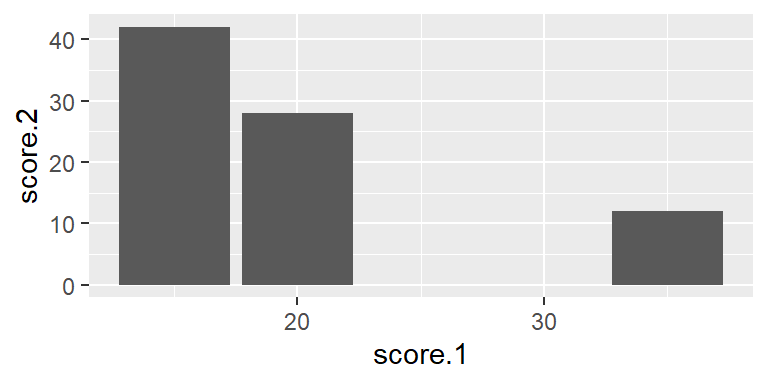
\includegraphics{05-ggplot2_files/figure-latex/unnamed-chunk-2-2.pdf}

\hypertarget{the-geom-layer}{%
\section{The geom layer}\label{the-geom-layer}}

The geom layer declares the type of plot to be produced. More on this in the next chapter.

\begin{Shaded}
\begin{Highlighting}[]
\CommentTok{\# adding the geom layer}
\FunctionTok{ggplot}\NormalTok{(}\AttributeTok{data =}\NormalTok{ gapminder\_2007, }\FunctionTok{aes}\NormalTok{(}\AttributeTok{y =}\NormalTok{ lifeExp, }\AttributeTok{x =}\NormalTok{ gdpPercap)) }\SpecialCharTok{+} 
  \FunctionTok{geom\_point}\NormalTok{()}
\end{Highlighting}
\end{Shaded}

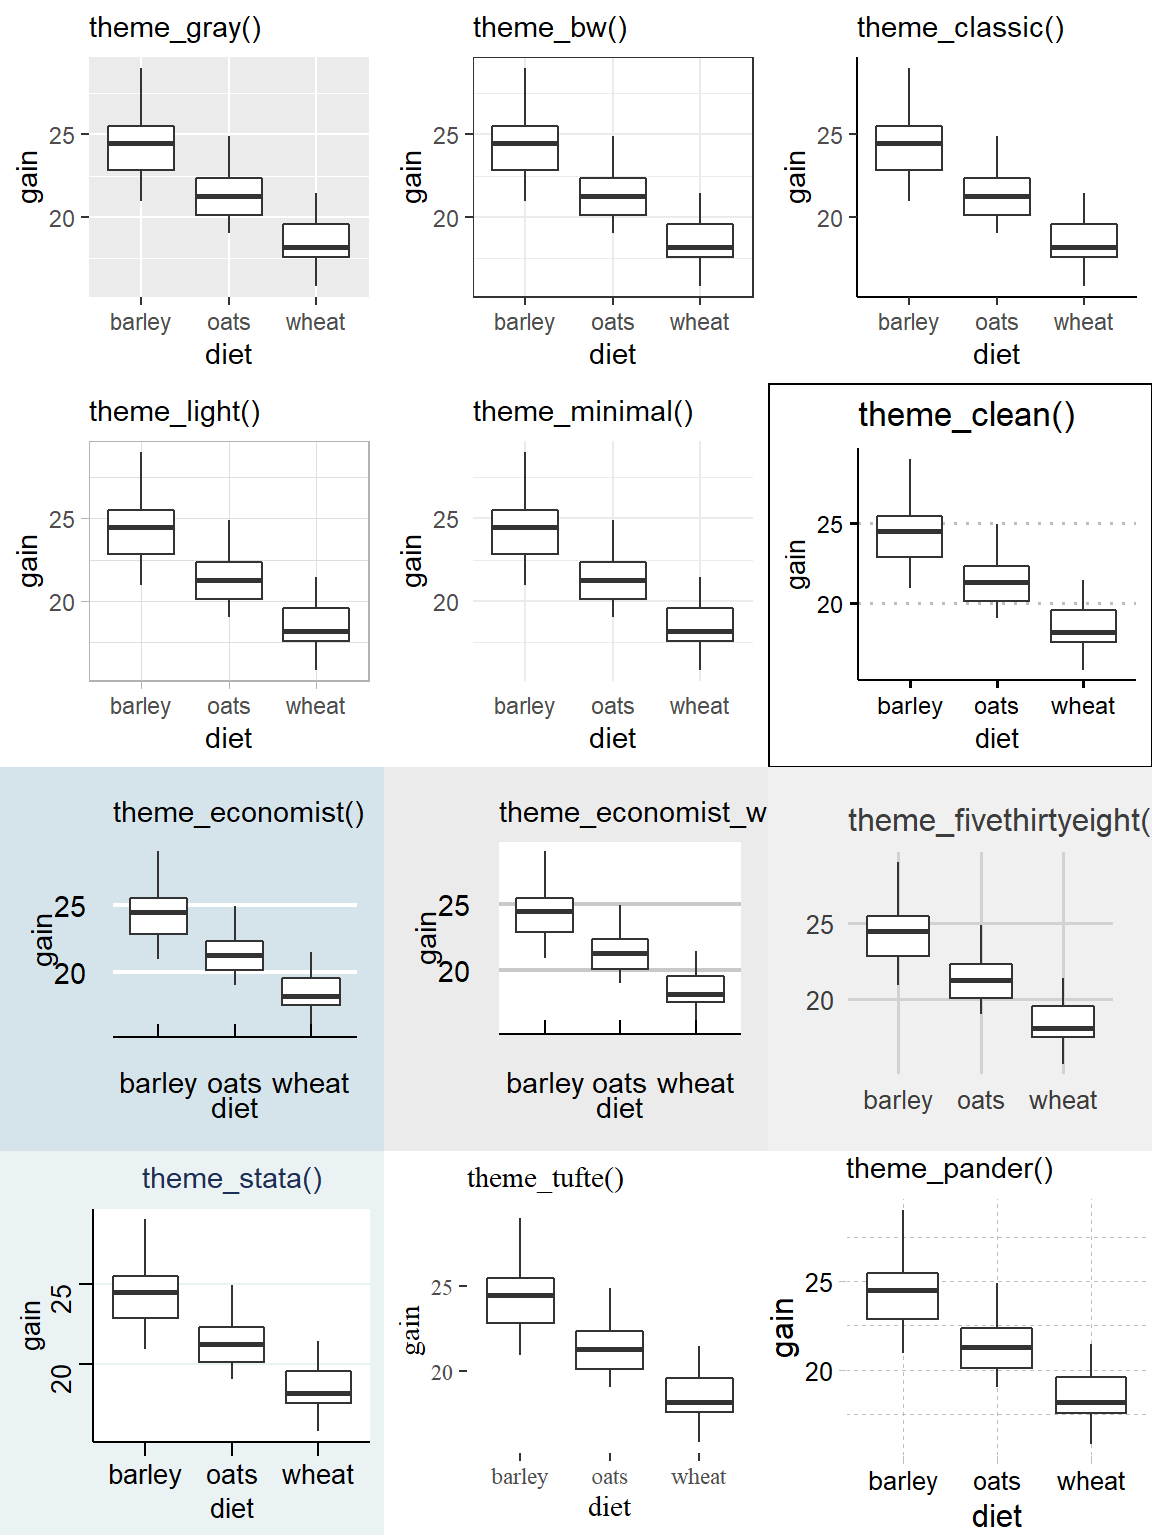
\includegraphics{05-ggplot2_files/figure-latex/unnamed-chunk-3-1.pdf}

\begin{Shaded}
\begin{Highlighting}[]

\CommentTok{\# Both data and axis can be declared within the geom layer.}
\FunctionTok{ggplot}\NormalTok{(}\AttributeTok{data =}\NormalTok{ gapminder\_2007) }\SpecialCharTok{+} 
  \FunctionTok{geom\_point}\NormalTok{(}\AttributeTok{mapping =} \FunctionTok{aes}\NormalTok{(}\AttributeTok{y =}\NormalTok{ lifeExp, }\AttributeTok{x =}\NormalTok{ gdpPercap))}
\end{Highlighting}
\end{Shaded}

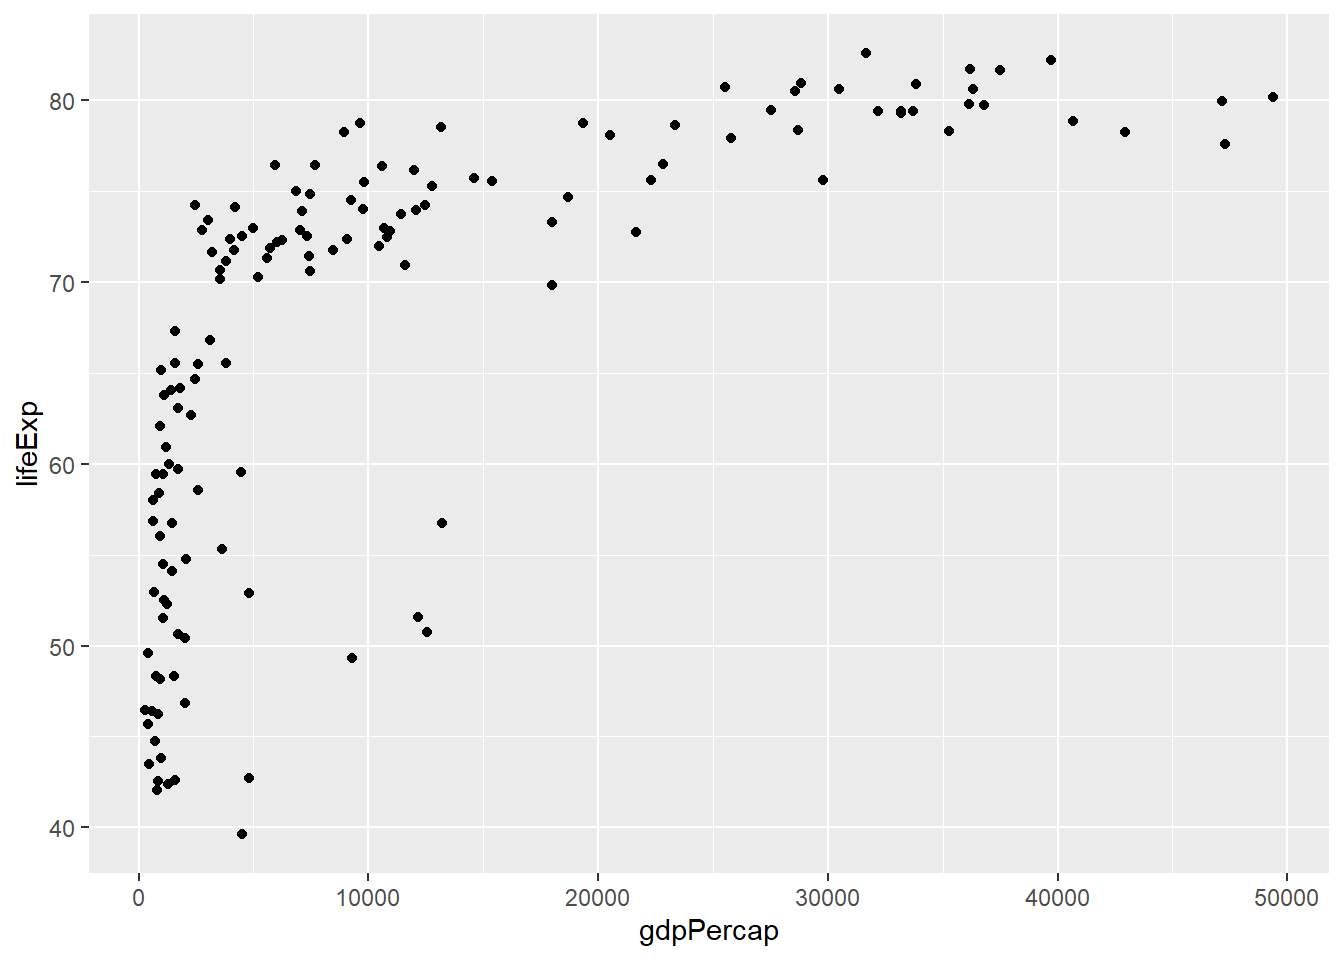
\includegraphics{05-ggplot2_files/figure-latex/unnamed-chunk-3-2.pdf}

\begin{Shaded}
\begin{Highlighting}[]

\FunctionTok{ggplot}\NormalTok{() }\SpecialCharTok{+} 
  \FunctionTok{geom\_point}\NormalTok{(}\AttributeTok{data =}\NormalTok{ gapminder\_2007, }\FunctionTok{aes}\NormalTok{(}\AttributeTok{y =}\NormalTok{ lifeExp, }\AttributeTok{x =}\NormalTok{ gdpPercap))}
\end{Highlighting}
\end{Shaded}

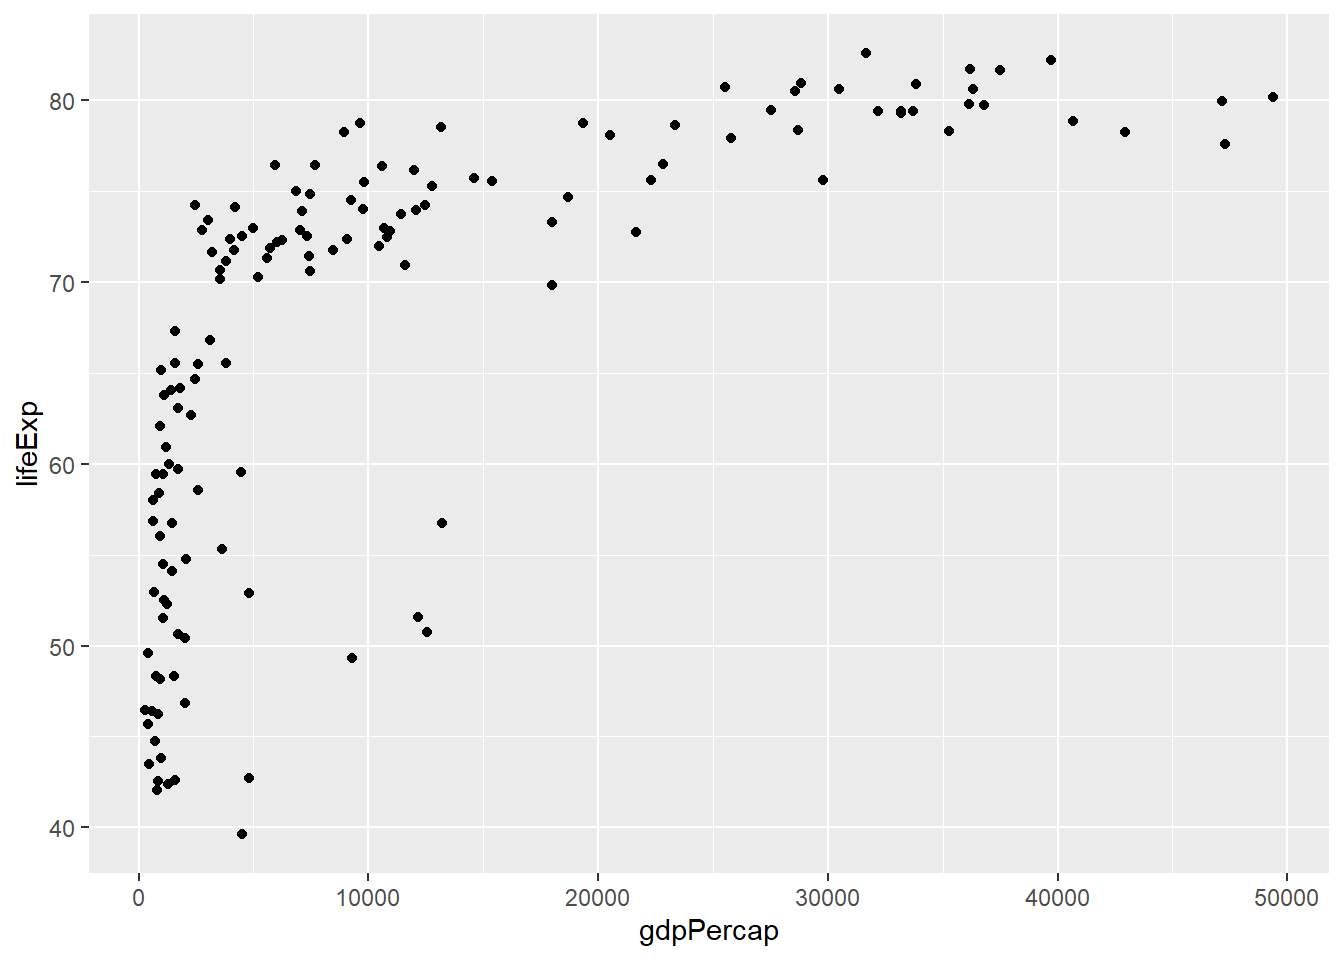
\includegraphics{05-ggplot2_files/figure-latex/unnamed-chunk-3-3.pdf}

\hypertarget{shape}{%
\section{Shape}\label{shape}}

Shapes are controlled using the argument shape.

\hypertarget{setting-shapes}{%
\subsection{Setting shapes}\label{setting-shapes}}

Shapes are set by passing shape to geom\_* but must be placed outside aes() as aes() is meant for mapping. Shape expects the same arguments as pch in base graphics that is, integers ranging from 1 to 25 or characters.

\begin{Shaded}
\begin{Highlighting}[]
\CommentTok{\# changing shapes}
\FunctionTok{ggplot}\NormalTok{(gapminder\_2007) }\SpecialCharTok{+} 
  \FunctionTok{geom\_point}\NormalTok{(}\FunctionTok{aes}\NormalTok{(}\AttributeTok{y =}\NormalTok{ lifeExp, }\AttributeTok{x =}\NormalTok{ gdpPercap), }\AttributeTok{shape =} \DecValTok{21}\NormalTok{)}
\end{Highlighting}
\end{Shaded}

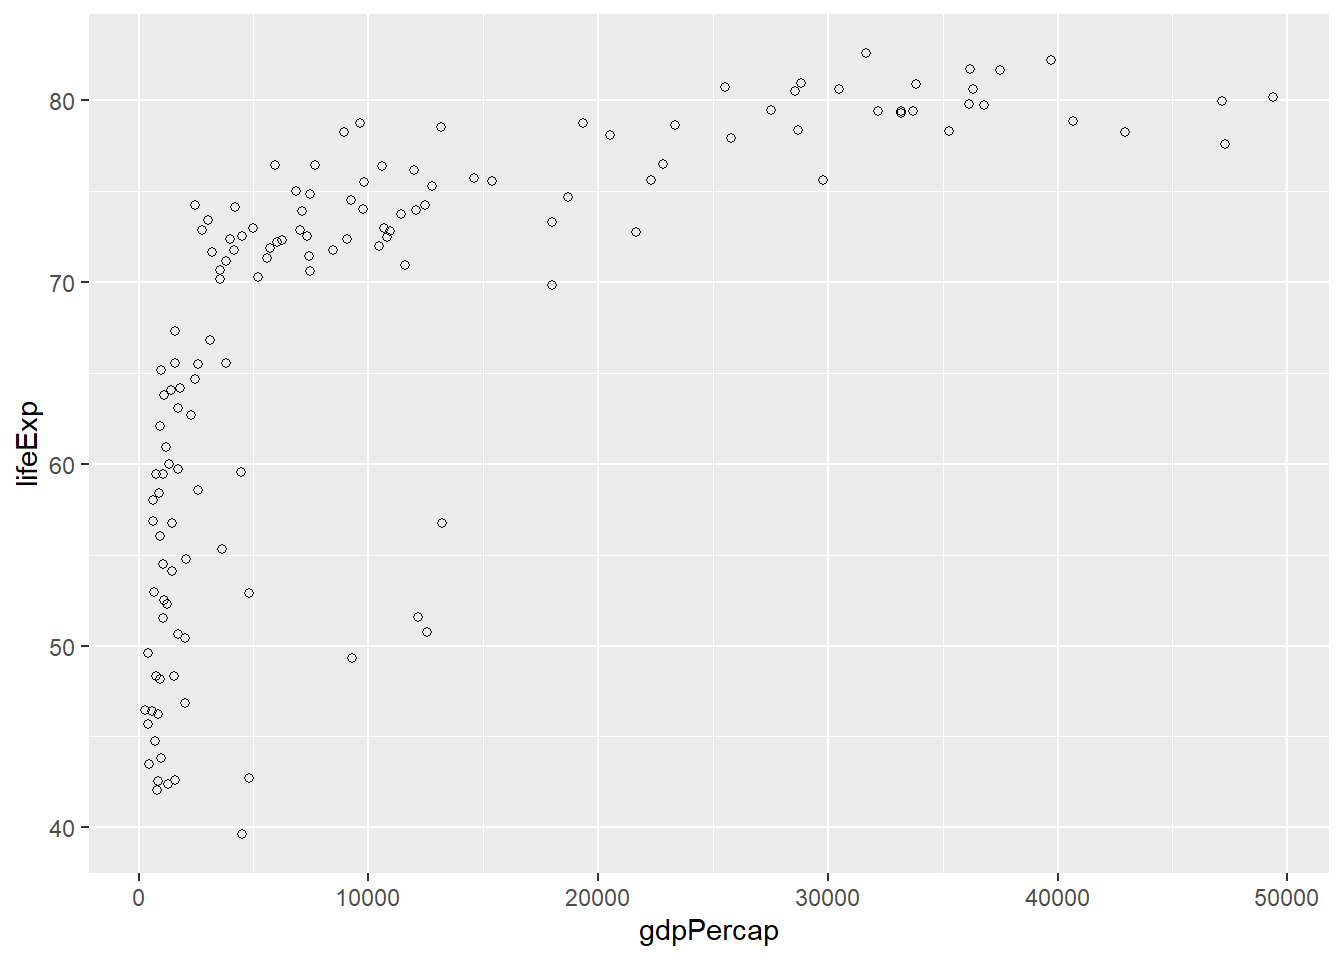
\includegraphics{05-ggplot2_files/figure-latex/unnamed-chunk-4-1.pdf}

\begin{Shaded}
\begin{Highlighting}[]
\CommentTok{\# using a character}
\FunctionTok{ggplot}\NormalTok{(gapminder\_2007) }\SpecialCharTok{+} 
  \FunctionTok{geom\_point}\NormalTok{(}\FunctionTok{aes}\NormalTok{(}\AttributeTok{y =}\NormalTok{ lifeExp, }\AttributeTok{x =}\NormalTok{ gdpPercap), }\AttributeTok{shape =} \StringTok{\textquotesingle{}*\textquotesingle{}}\NormalTok{)}
\end{Highlighting}
\end{Shaded}

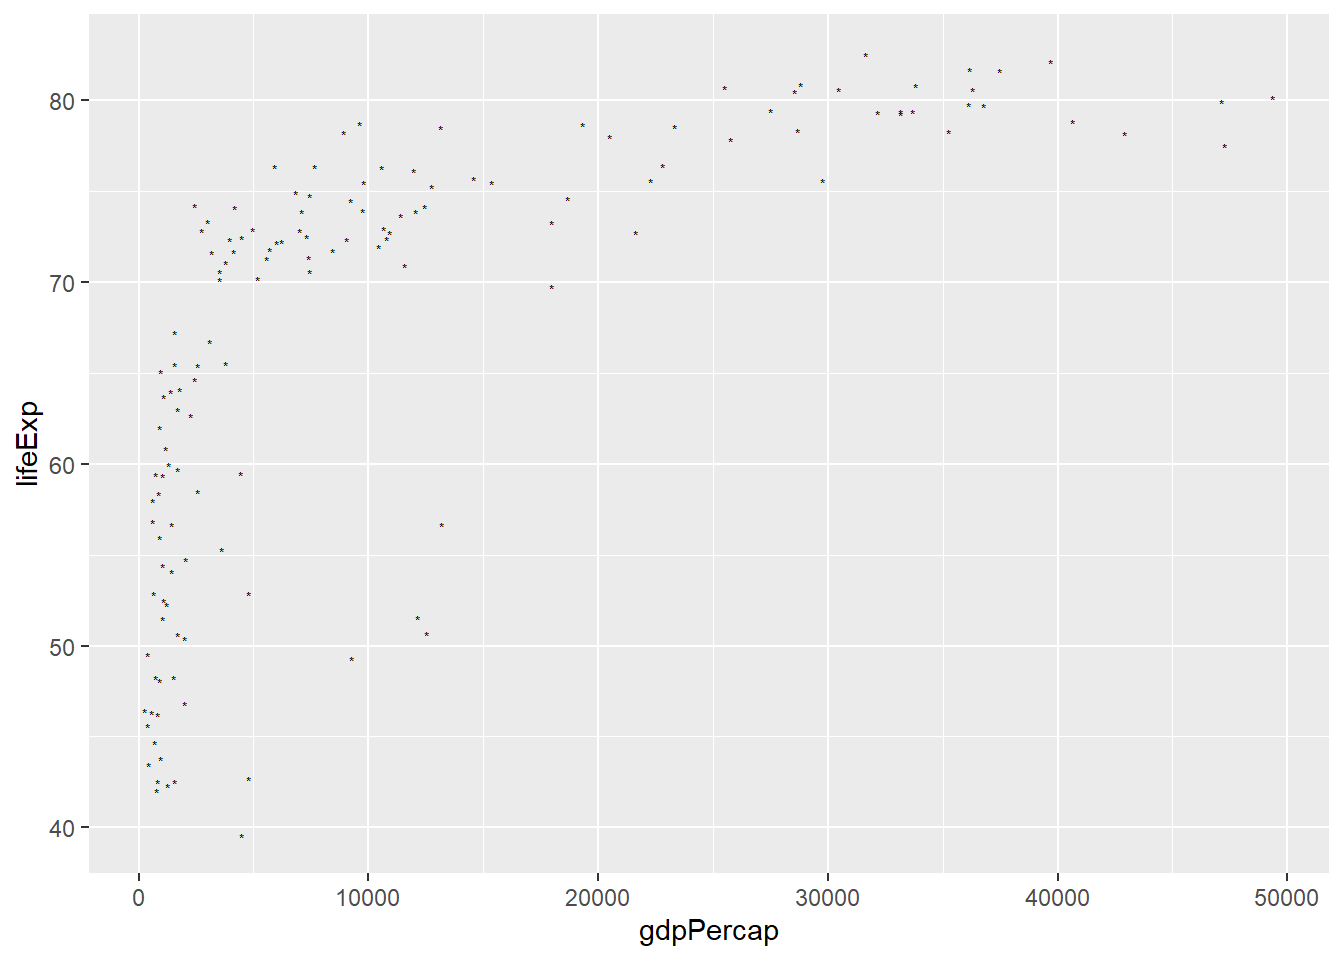
\includegraphics{05-ggplot2_files/figure-latex/unnamed-chunk-4-2.pdf}

\hypertarget{mapping-shapes}{%
\subsection{Mapping shapes}\label{mapping-shapes}}

The mapping of data to shapes allows us to have shapes by groups or categories for example having different shapes for different continents. To map data to shapes, the shape argument is passed a categorical variable and placed within \texttt{aes()}.

\begin{Shaded}
\begin{Highlighting}[]
\CommentTok{\# shapes by continent}
\FunctionTok{ggplot}\NormalTok{(gapminder\_2007) }\SpecialCharTok{+} 
  \FunctionTok{geom\_point}\NormalTok{(}\FunctionTok{aes}\NormalTok{(}\AttributeTok{y =}\NormalTok{ lifeExp, }\AttributeTok{x =}\NormalTok{ gdpPercap, }\AttributeTok{shape =}\NormalTok{ continent))}
\end{Highlighting}
\end{Shaded}

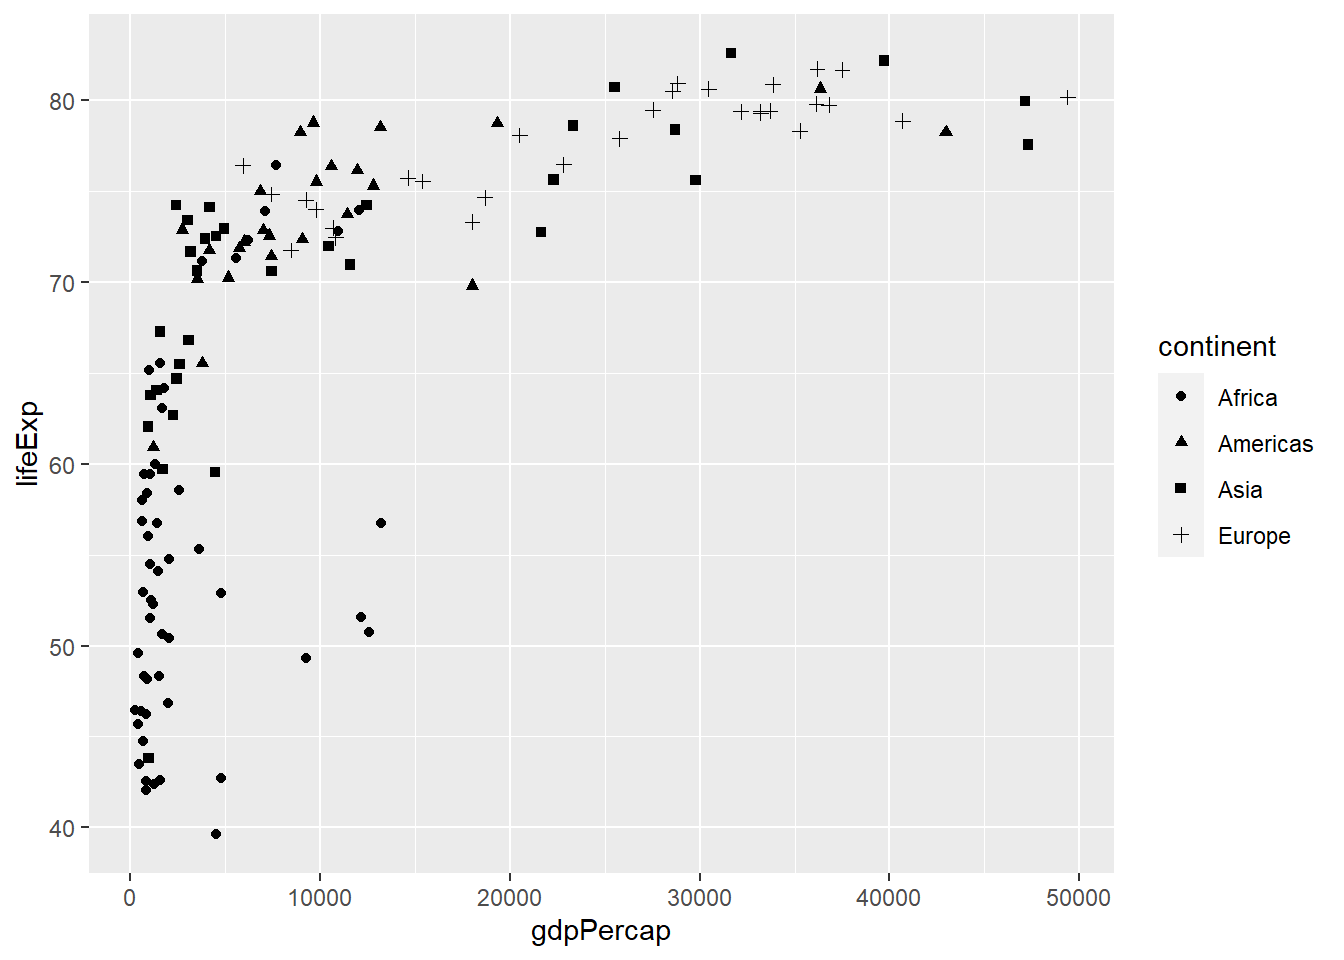
\includegraphics{05-ggplot2_files/figure-latex/unnamed-chunk-5-1.pdf}

\hypertarget{scaling-shapes}{%
\subsection{Scaling shapes}\label{scaling-shapes}}

The function \texttt{scale\_shape\_manual()} is used to scale shapes that is determine the shapes to use in the plot.

\begin{Shaded}
\begin{Highlighting}[]
\CommentTok{\# using shapes ranging from 15 to 19}
\FunctionTok{ggplot}\NormalTok{(gapminder\_2007) }\SpecialCharTok{+} 
  \FunctionTok{geom\_point}\NormalTok{(}\FunctionTok{aes}\NormalTok{(}\AttributeTok{y =}\NormalTok{ lifeExp, }\AttributeTok{x =}\NormalTok{ gdpPercap, }\AttributeTok{shape =}\NormalTok{ continent)) }\SpecialCharTok{+}
  \FunctionTok{scale\_shape\_manual}\NormalTok{(}\AttributeTok{values =} \DecValTok{15}\SpecialCharTok{:}\DecValTok{19}\NormalTok{)}
\end{Highlighting}
\end{Shaded}

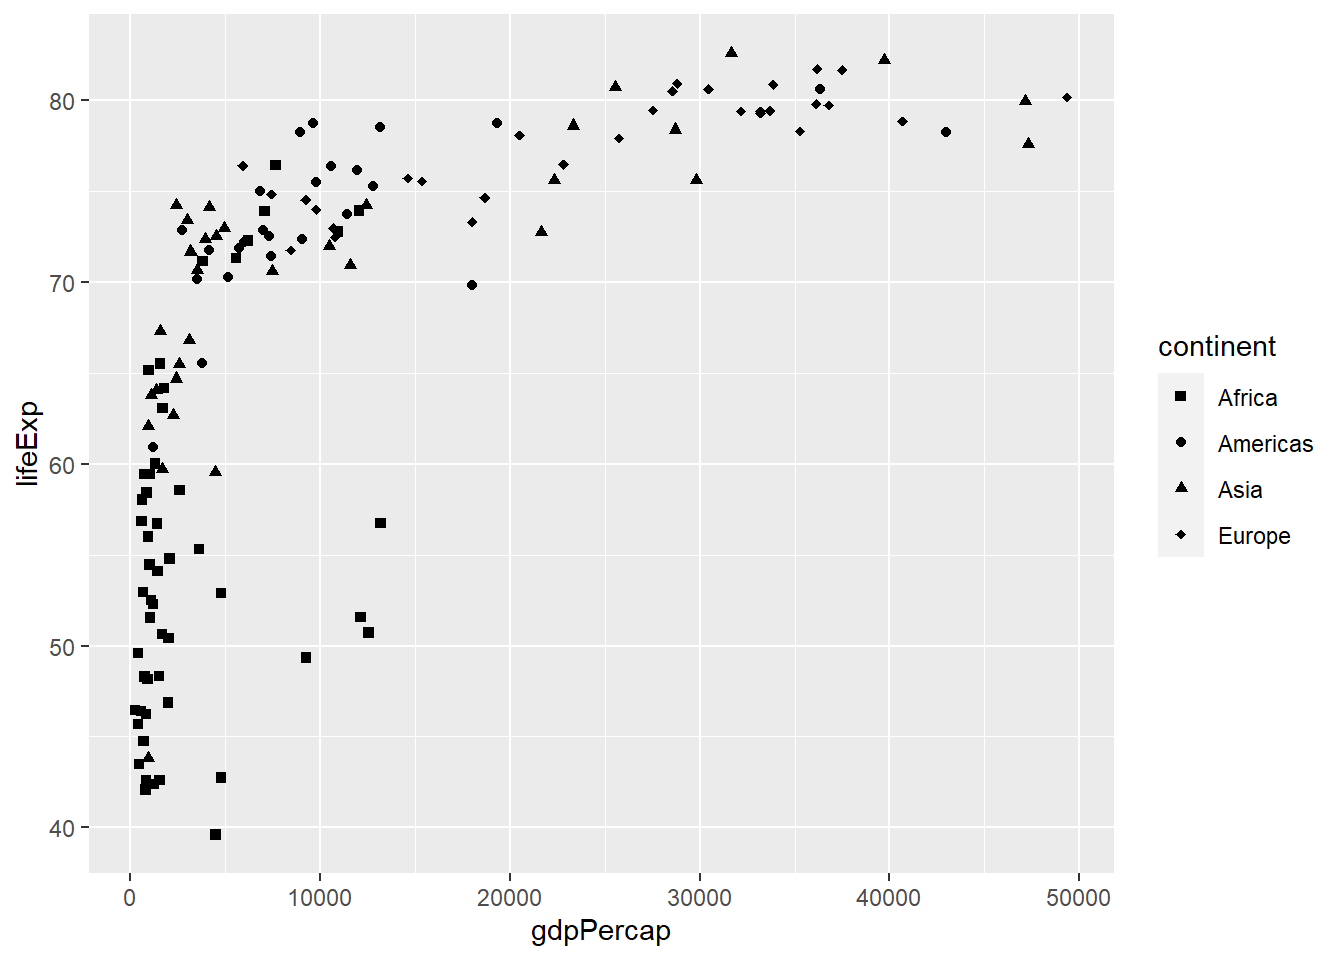
\includegraphics{05-ggplot2_files/figure-latex/unnamed-chunk-6-1.pdf}

\hypertarget{size}{%
\section{Size}\label{size}}

size is controlled using the argument \texttt{size=}.

\hypertarget{setting-size}{%
\subsection{Setting size}\label{setting-size}}

\begin{Shaded}
\begin{Highlighting}[]
\CommentTok{\# adjusting size}
\FunctionTok{ggplot}\NormalTok{(gapminder\_2007) }\SpecialCharTok{+} 
  \FunctionTok{geom\_point}\NormalTok{(}\FunctionTok{aes}\NormalTok{(}\AttributeTok{y =}\NormalTok{ lifeExp, }\AttributeTok{x =}\NormalTok{ gdpPercap), }\AttributeTok{size =} \DecValTok{3}\NormalTok{)}
\end{Highlighting}
\end{Shaded}

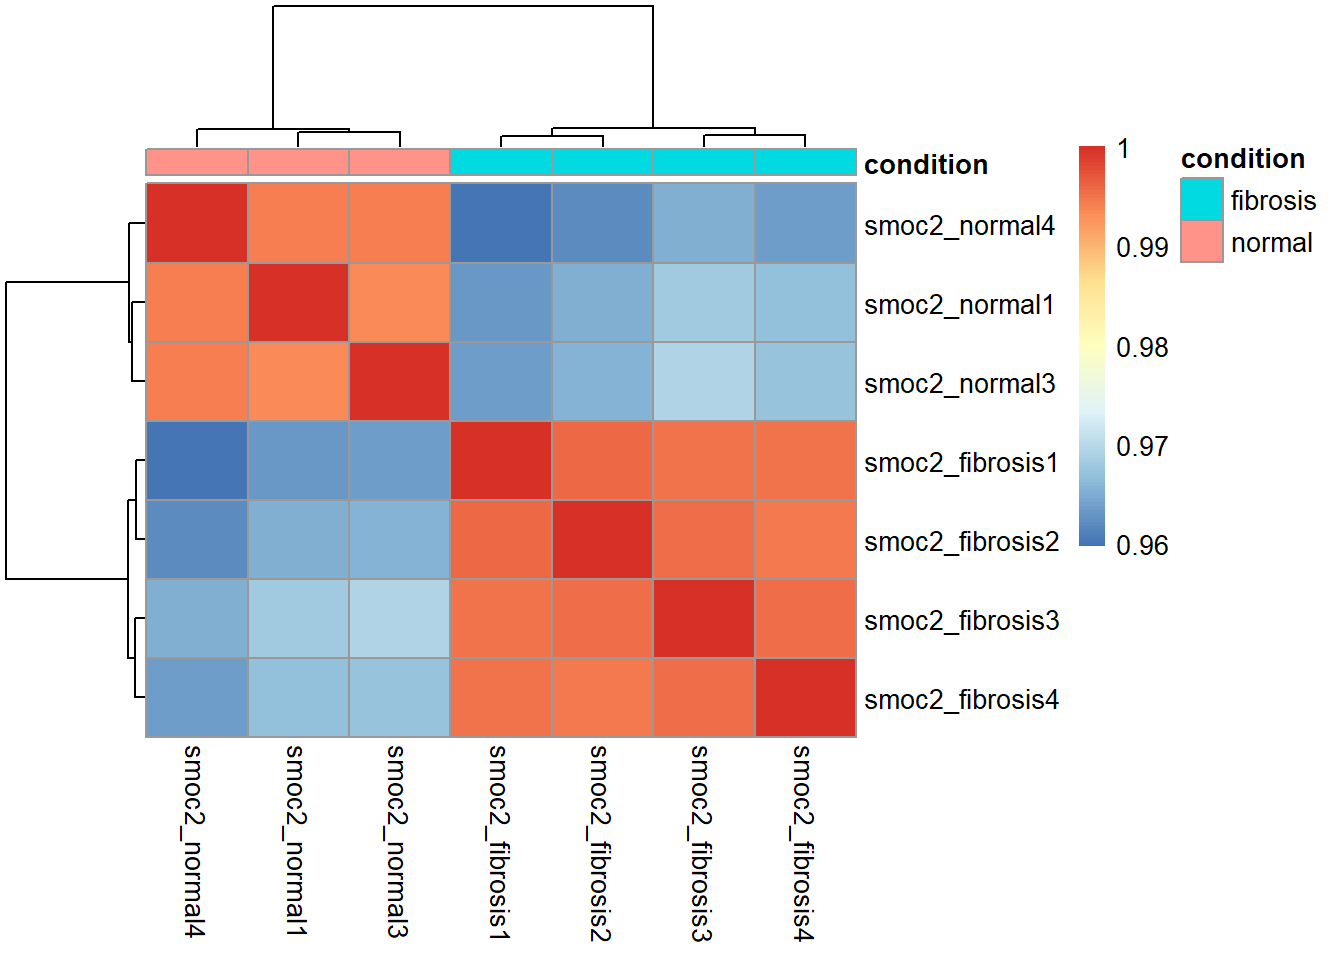
\includegraphics{05-ggplot2_files/figure-latex/unnamed-chunk-7-1.pdf}

\hypertarget{mapping-size}{%
\subsection{Mapping size}\label{mapping-size}}

Size is mapped by assigning them a continuous variable and placing them within \texttt{aes()}.

\begin{Shaded}
\begin{Highlighting}[]
\CommentTok{\# size by population}
\FunctionTok{ggplot}\NormalTok{(gapminder\_2007) }\SpecialCharTok{+} 
  \FunctionTok{geom\_point}\NormalTok{(}\FunctionTok{aes}\NormalTok{(}\AttributeTok{y =}\NormalTok{ lifeExp, }\AttributeTok{x =}\NormalTok{ gdpPercap, }\AttributeTok{size =}\NormalTok{ pop), }\AttributeTok{shape =} \DecValTok{21}\NormalTok{)}
\end{Highlighting}
\end{Shaded}

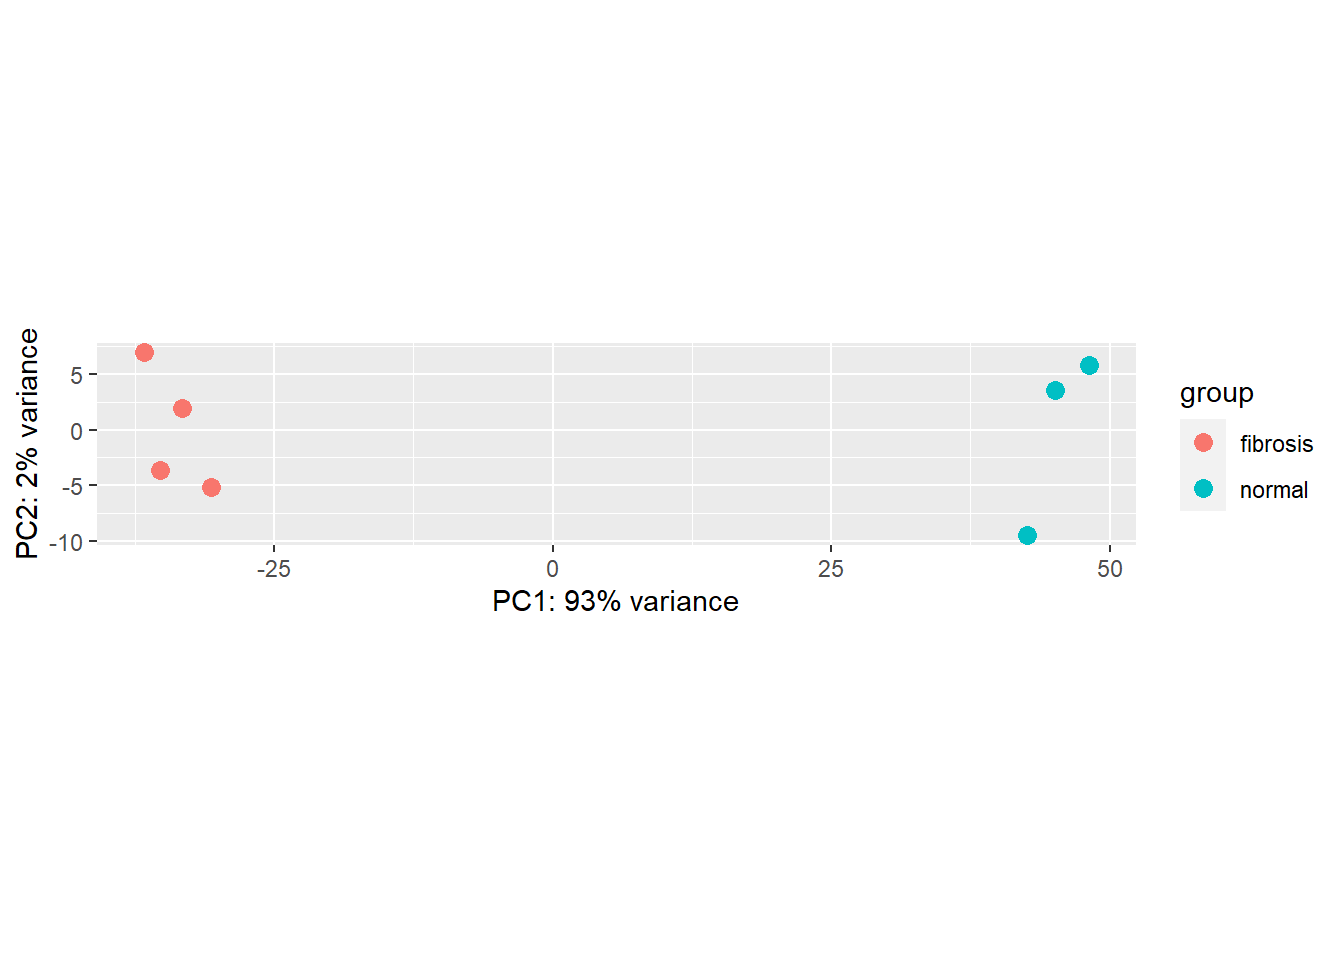
\includegraphics{05-ggplot2_files/figure-latex/unnamed-chunk-8-1.pdf}

\hypertarget{colour}{%
\section{Colour}\label{colour}}

Colour is controlled using the argument \texttt{color=} or \texttt{colour=}.

\hypertarget{setting-colours}{%
\subsection{Setting colours}\label{setting-colours}}

\begin{Shaded}
\begin{Highlighting}[]
\FunctionTok{ggplot}\NormalTok{(gapminder\_2007) }\SpecialCharTok{+} 
  \FunctionTok{geom\_point}\NormalTok{(}\FunctionTok{aes}\NormalTok{(}\AttributeTok{y =}\NormalTok{ lifeExp, }\AttributeTok{x =}\NormalTok{ gdpPercap), }\AttributeTok{colour =} \StringTok{\textquotesingle{}darkblue\textquotesingle{}}\NormalTok{, }\AttributeTok{size =} \DecValTok{3}\NormalTok{, }\AttributeTok{shape =} \DecValTok{19}\NormalTok{)}
\end{Highlighting}
\end{Shaded}

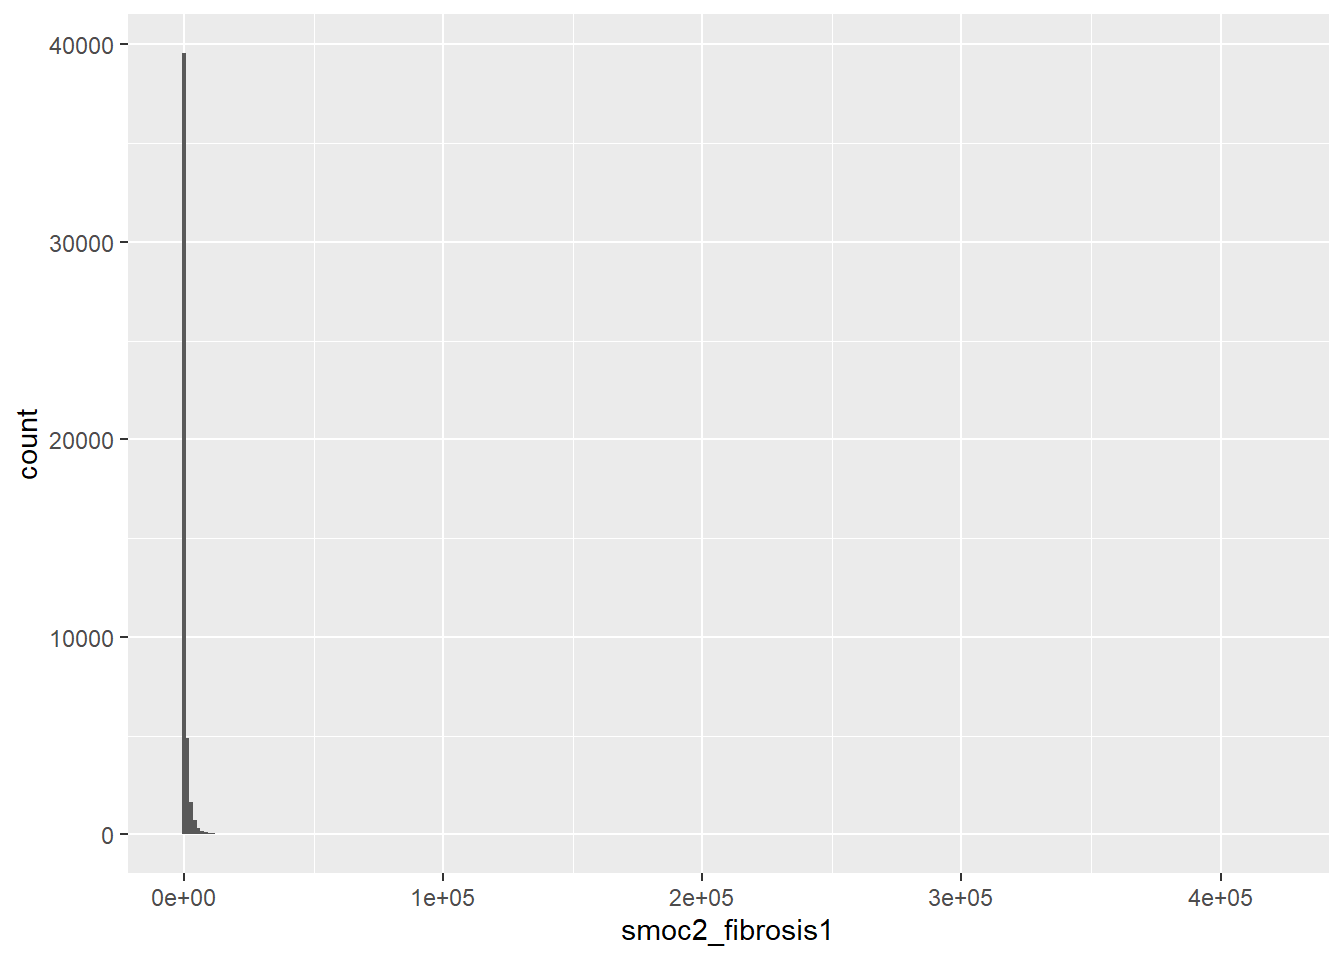
\includegraphics{05-ggplot2_files/figure-latex/unnamed-chunk-9-1.pdf}

\hypertarget{fill-vs-colour}{%
\subsection{Fill vs colour}\label{fill-vs-colour}}

With shapes between 21 to 25 and bars, the argument fill is used to fill shapes while colour is used to colour borders (outlines).

\begin{Shaded}
\begin{Highlighting}[]
\CommentTok{\# using colour and fill}
\FunctionTok{ggplot}\NormalTok{(gapminder\_2007) }\SpecialCharTok{+} 
\FunctionTok{geom\_point}\NormalTok{(}\FunctionTok{aes}\NormalTok{(}\AttributeTok{y =}\NormalTok{ lifeExp, }\AttributeTok{x =}\NormalTok{ gdpPercap), }\AttributeTok{colour =} \StringTok{\textquotesingle{}darkblue\textquotesingle{}}\NormalTok{, }\AttributeTok{fill =} \StringTok{\textquotesingle{}lightblue\textquotesingle{}}\NormalTok{, }
           \AttributeTok{size =} \DecValTok{3}\NormalTok{, }\AttributeTok{shape =} \DecValTok{21}\NormalTok{)}
\end{Highlighting}
\end{Shaded}

\includegraphics{05-ggplot2_files/figure-latex/unnamed-chunk-10-1.pdf}

\hypertarget{stroke}{%
\subsection{Stroke}\label{stroke}}

The border or outline size is controlled using the argument \texttt{stroke=}.

\begin{Shaded}
\begin{Highlighting}[]
\FunctionTok{ggplot}\NormalTok{(gapminder\_2007) }\SpecialCharTok{+} 
  \FunctionTok{geom\_point}\NormalTok{(}\FunctionTok{aes}\NormalTok{(}\AttributeTok{y =}\NormalTok{ lifeExp, }\AttributeTok{x =}\NormalTok{ gdpPercap), }\AttributeTok{colour =} \StringTok{\textquotesingle{}darkblue\textquotesingle{}}\NormalTok{, }\AttributeTok{fill =} \StringTok{\textquotesingle{}lightblue\textquotesingle{}}\NormalTok{, }
           \AttributeTok{size =} \DecValTok{3}\NormalTok{, }\AttributeTok{shape =} \DecValTok{21}\NormalTok{, }\AttributeTok{stroke =} \DecValTok{1}\NormalTok{)}
\end{Highlighting}
\end{Shaded}

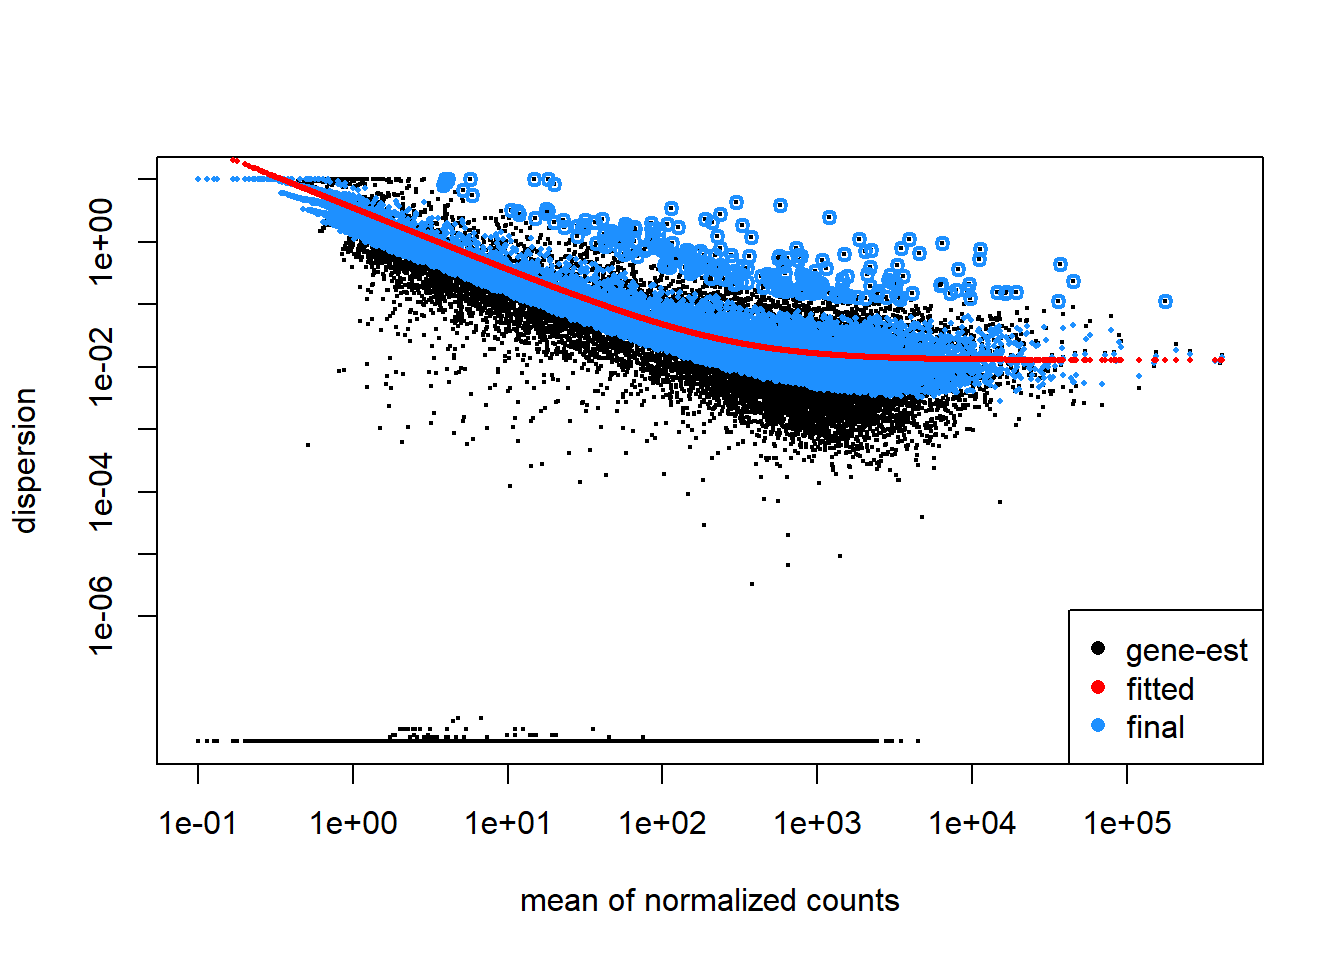
\includegraphics{05-ggplot2_files/figure-latex/unnamed-chunk-11-1.pdf}

\hypertarget{transparency}{%
\subsection{Transparency}\label{transparency}}

Transparency is controlled by the argument \texttt{alpha=}. It accepts values from 0 to 1.

\begin{Shaded}
\begin{Highlighting}[]
\FunctionTok{ggplot}\NormalTok{(gapminder\_2007) }\SpecialCharTok{+} 
  \FunctionTok{geom\_point}\NormalTok{(}\FunctionTok{aes}\NormalTok{(}\AttributeTok{y =}\NormalTok{ lifeExp, }\AttributeTok{x =}\NormalTok{ gdpPercap), }
           \AttributeTok{colour =} \StringTok{\textquotesingle{}darkblue\textquotesingle{}}\NormalTok{, }\AttributeTok{fill =} \StringTok{\textquotesingle{}lightblue\textquotesingle{}}\NormalTok{, }\AttributeTok{size =} \DecValTok{3}\NormalTok{, }\AttributeTok{shape =} \DecValTok{21}\NormalTok{, }
           \AttributeTok{stroke =} \DecValTok{1}\NormalTok{, }\AttributeTok{alpha =} \FloatTok{0.5}\NormalTok{)}
\end{Highlighting}
\end{Shaded}

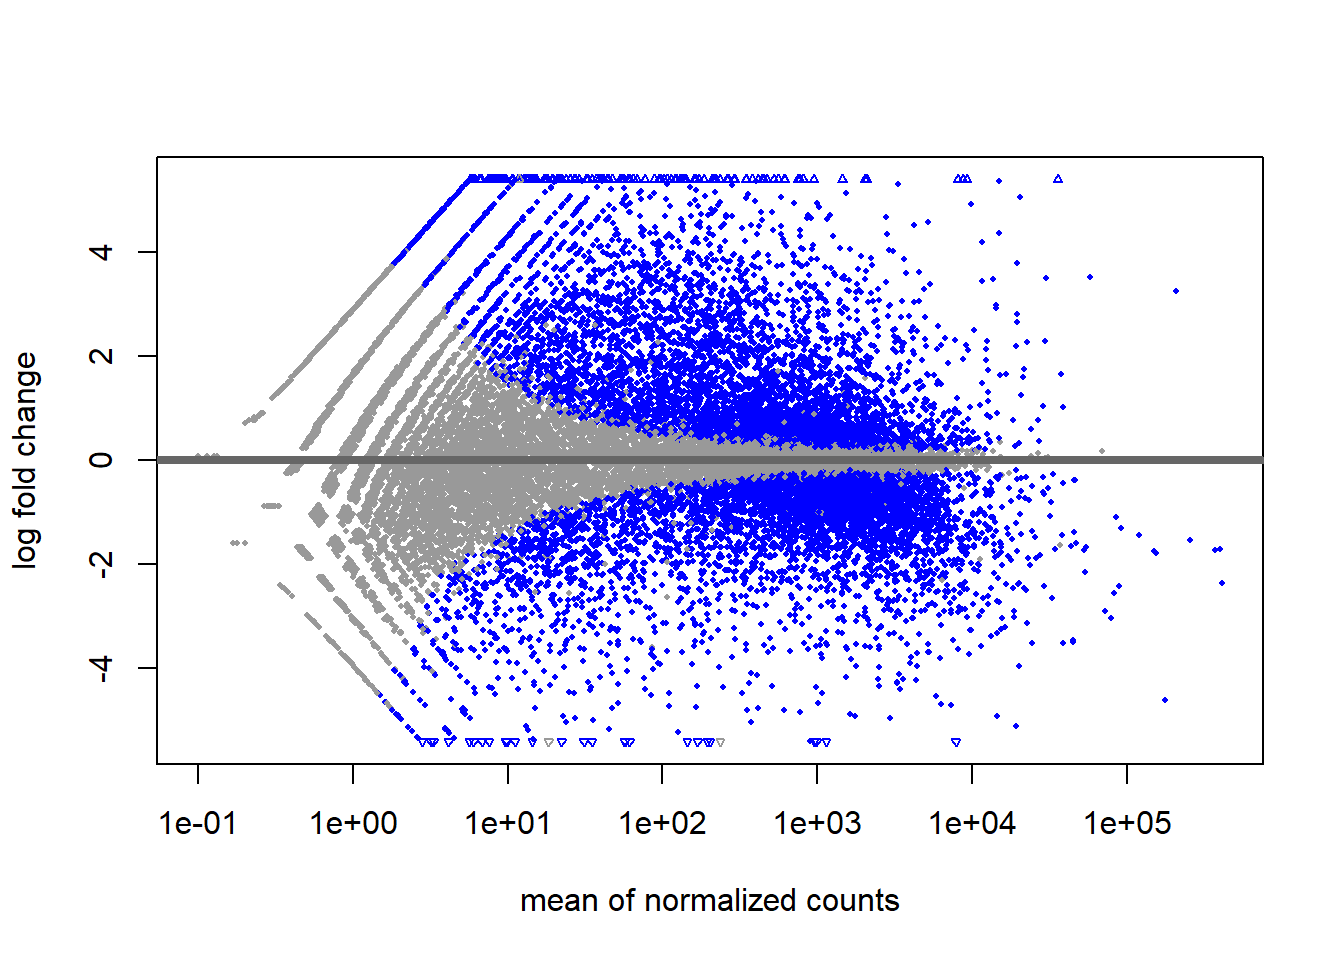
\includegraphics{05-ggplot2_files/figure-latex/unnamed-chunk-12-1.pdf}

\hypertarget{mapping-colours-to-discrete-variables}{%
\subsection{Mapping colours to discrete variables}\label{mapping-colours-to-discrete-variables}}

As with shapes, colours are mapped by assigning a discrete variable to them and placing them within \texttt{aes()}.

\begin{Shaded}
\begin{Highlighting}[]
\CommentTok{\# colour by continent}
\FunctionTok{ggplot}\NormalTok{(gapminder\_2007) }\SpecialCharTok{+} 
  \FunctionTok{geom\_point}\NormalTok{(}\FunctionTok{aes}\NormalTok{(}\AttributeTok{y =}\NormalTok{ lifeExp, }\AttributeTok{x =}\NormalTok{ gdpPercap, }\AttributeTok{colour =}\NormalTok{ continent), }\AttributeTok{size =} \DecValTok{3}\NormalTok{, }
             \AttributeTok{shape =} \DecValTok{19}\NormalTok{, }\AttributeTok{alpha =} \FloatTok{0.5}\NormalTok{)}
\end{Highlighting}
\end{Shaded}

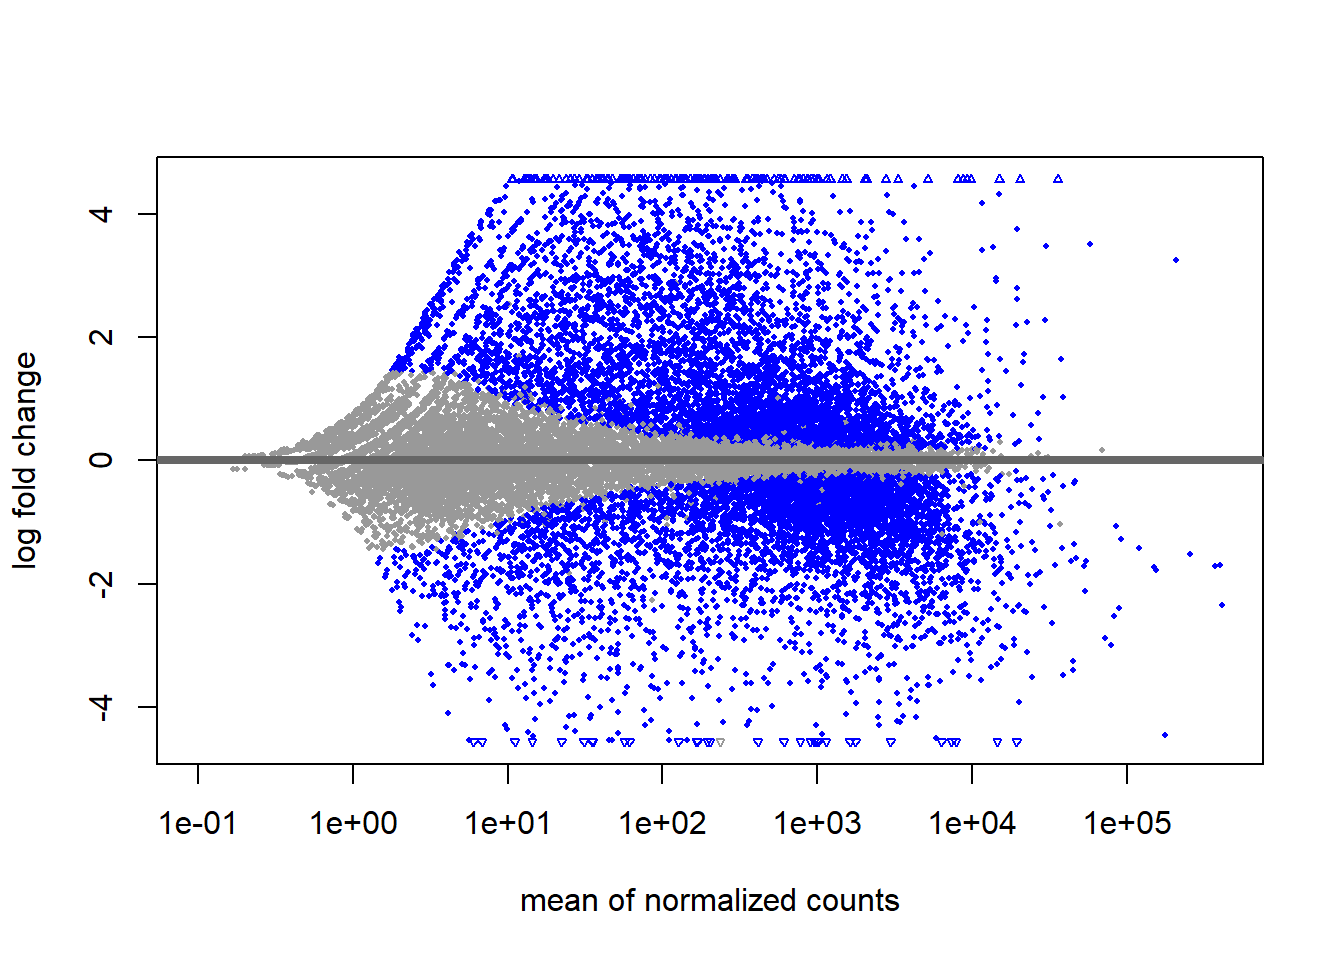
\includegraphics{05-ggplot2_files/figure-latex/unnamed-chunk-13-1.pdf}

\begin{Shaded}
\begin{Highlighting}[]
\CommentTok{\# fill by continent}
\FunctionTok{ggplot}\NormalTok{(gapminder\_2007) }\SpecialCharTok{+} 
  \FunctionTok{geom\_point}\NormalTok{(}\FunctionTok{aes}\NormalTok{(}\AttributeTok{y =}\NormalTok{ lifeExp, }\AttributeTok{x =}\NormalTok{ gdpPercap, }\AttributeTok{fill =}\NormalTok{ continent), }
             \AttributeTok{colour =} \StringTok{\textquotesingle{}darkblue\textquotesingle{}}\NormalTok{, }\AttributeTok{size =} \DecValTok{4}\NormalTok{, }\AttributeTok{shape =} \DecValTok{21}\NormalTok{, }\AttributeTok{alpha =} \FloatTok{0.5}\NormalTok{, }\AttributeTok{stroke =} \DecValTok{1}\NormalTok{)}
\end{Highlighting}
\end{Shaded}

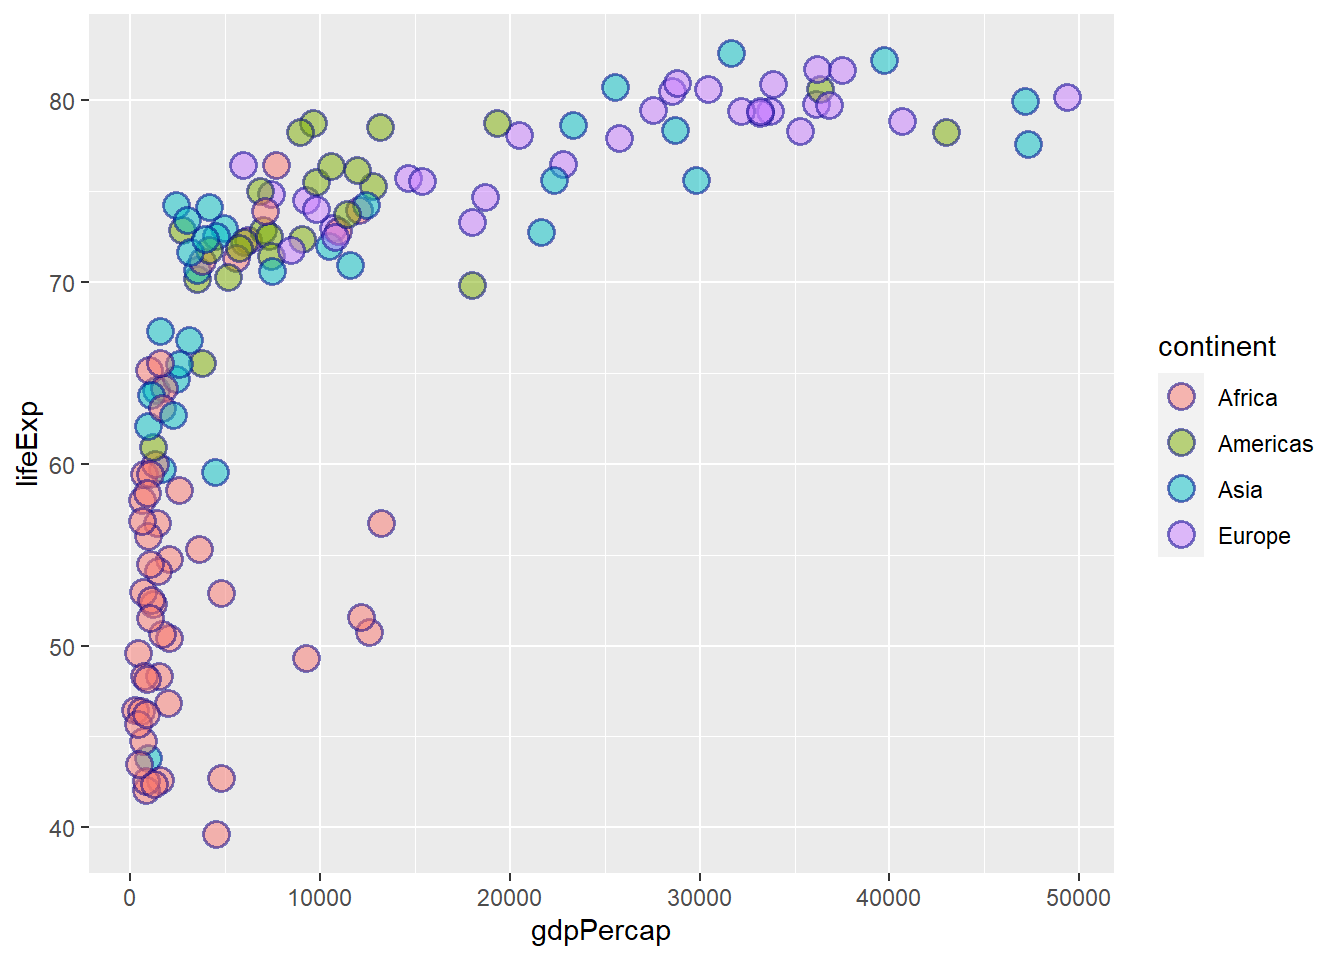
\includegraphics{05-ggplot2_files/figure-latex/unnamed-chunk-13-2.pdf}

\hypertarget{default-colours}{%
\subsection{Default colours}\label{default-colours}}

The functions \texttt{scale\_colour\_hue()} and \texttt{scale\_fill\_hue()} sets the default colour and fill scale for discrete variables.

\begin{Shaded}
\begin{Highlighting}[]
\FunctionTok{ggplot}\NormalTok{(gapminder\_2007) }\SpecialCharTok{+} 
  \FunctionTok{geom\_point}\NormalTok{(}\FunctionTok{aes}\NormalTok{(}\AttributeTok{y =}\NormalTok{ lifeExp, }\AttributeTok{x =}\NormalTok{ gdpPercap, }\AttributeTok{colour =}\NormalTok{ continent), }\AttributeTok{size =} \DecValTok{3}\NormalTok{, }
             \AttributeTok{shape =} \DecValTok{19}\NormalTok{, }\AttributeTok{alpha =} \FloatTok{0.5}\NormalTok{) }\SpecialCharTok{+}
  \FunctionTok{scale\_colour\_hue}\NormalTok{()}
\end{Highlighting}
\end{Shaded}

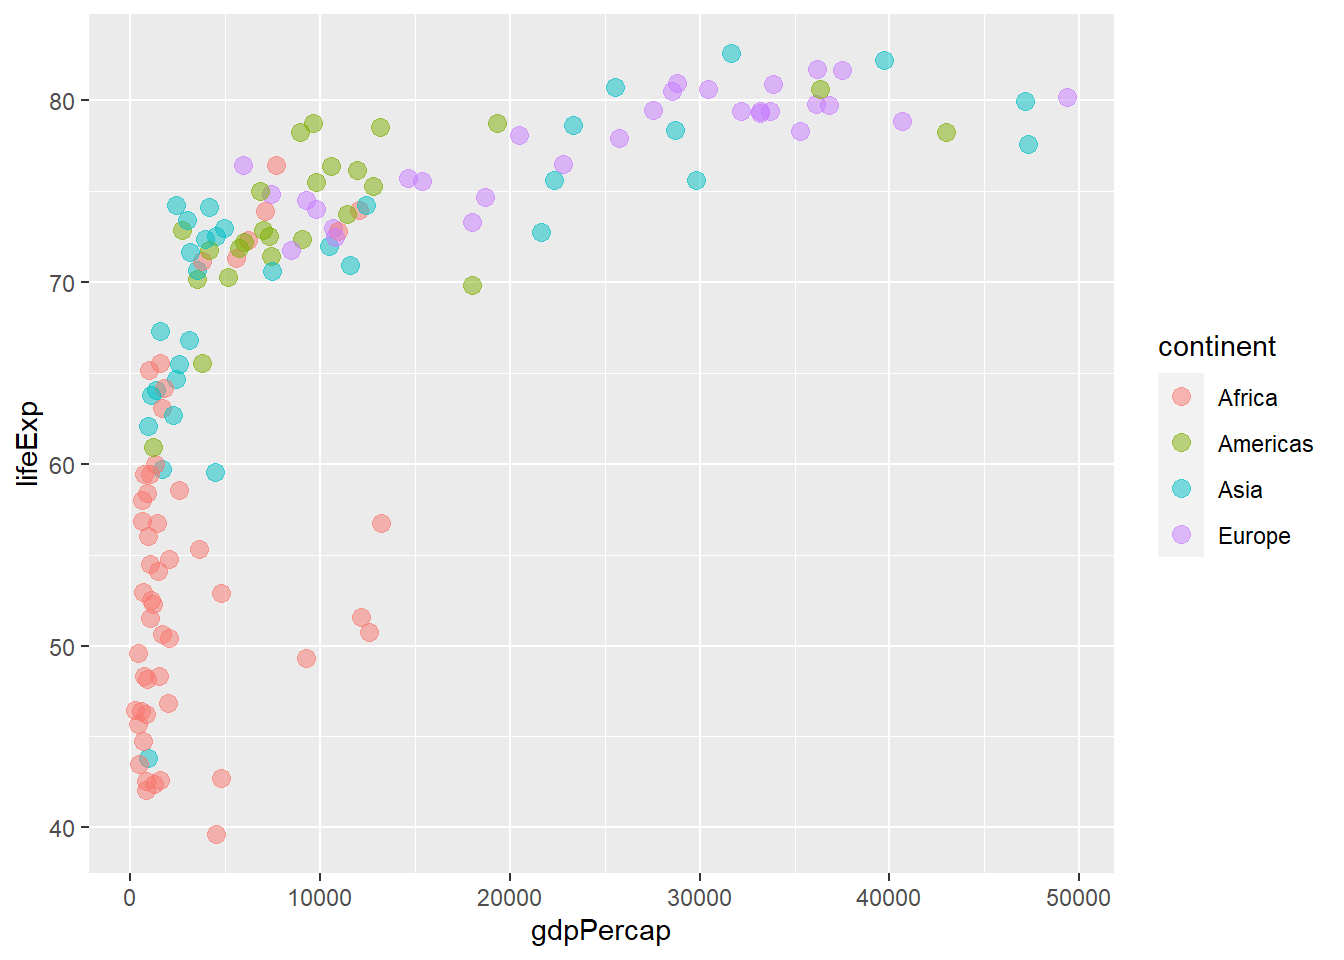
\includegraphics{05-ggplot2_files/figure-latex/unnamed-chunk-14-1.pdf}

\begin{Shaded}
\begin{Highlighting}[]
\CommentTok{\# Adjust luminosity and chroma}
\FunctionTok{ggplot}\NormalTok{(gapminder\_2007) }\SpecialCharTok{+} 
  \FunctionTok{geom\_point}\NormalTok{(}\FunctionTok{aes}\NormalTok{(}\AttributeTok{y =}\NormalTok{ lifeExp, }\AttributeTok{x =}\NormalTok{ gdpPercap, }\AttributeTok{colour =}\NormalTok{ continent), }\AttributeTok{size =} \DecValTok{3}\NormalTok{, }
             \AttributeTok{shape =} \DecValTok{19}\NormalTok{, }\AttributeTok{alpha =} \FloatTok{0.5}\NormalTok{) }\SpecialCharTok{+}
  \FunctionTok{scale\_colour\_hue}\NormalTok{(}\AttributeTok{l =} \DecValTok{70}\NormalTok{, }\AttributeTok{c =} \DecValTok{150}\NormalTok{)}
\end{Highlighting}
\end{Shaded}

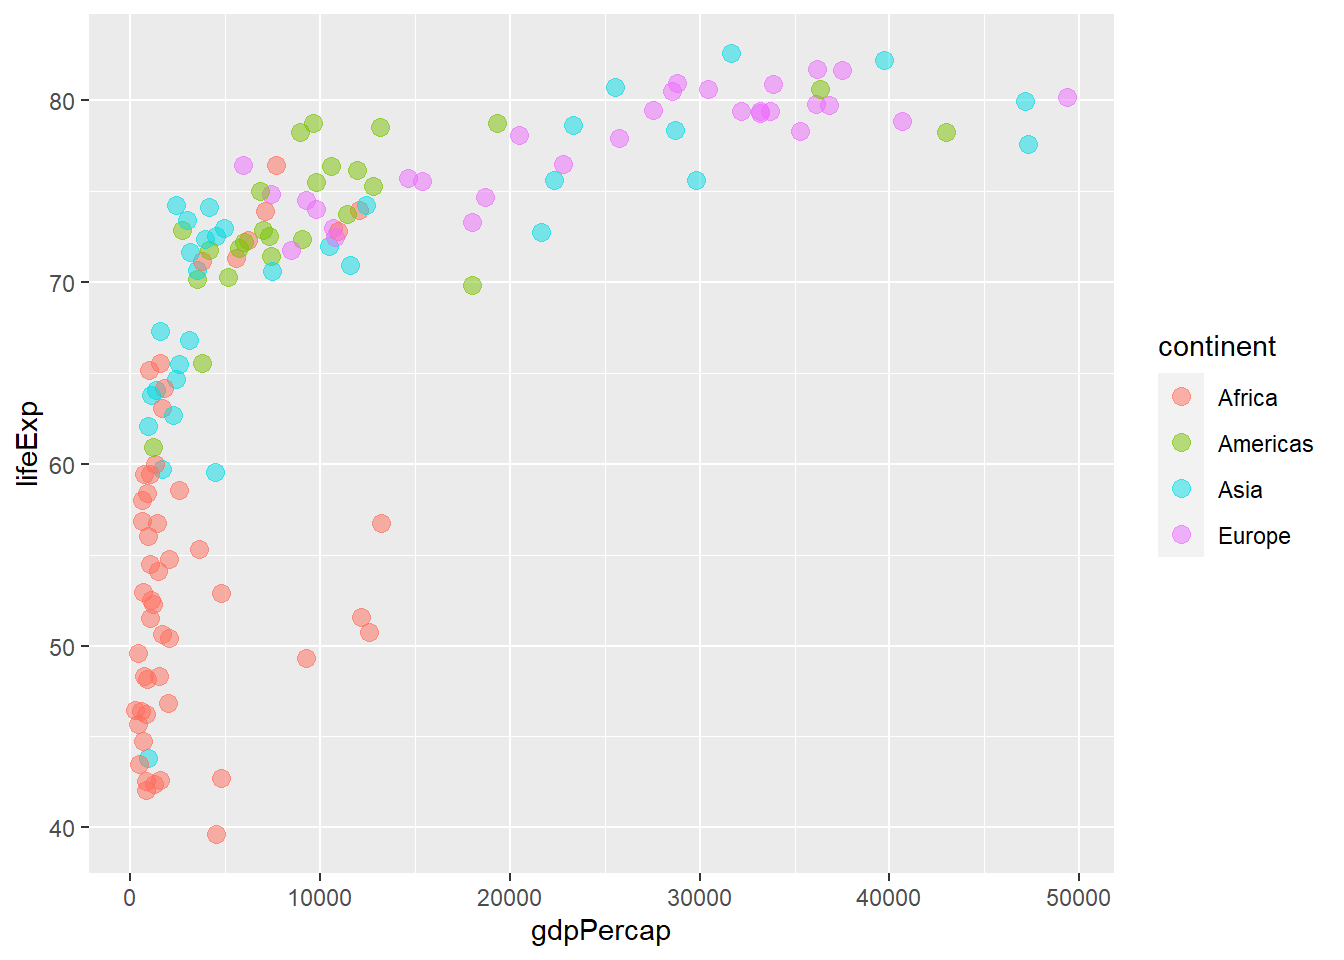
\includegraphics{05-ggplot2_files/figure-latex/unnamed-chunk-15-1.pdf}

\begin{Shaded}
\begin{Highlighting}[]


\CommentTok{\# Changing the range of hues used}
\FunctionTok{ggplot}\NormalTok{(gapminder\_2007) }\SpecialCharTok{+} 
  \FunctionTok{geom\_point}\NormalTok{(}\FunctionTok{aes}\NormalTok{(}\AttributeTok{y =}\NormalTok{ lifeExp, }\AttributeTok{x =}\NormalTok{ gdpPercap, }\AttributeTok{colour =}\NormalTok{ continent), }\AttributeTok{size =} \DecValTok{3}\NormalTok{, }
             \AttributeTok{shape =} \DecValTok{19}\NormalTok{, }\AttributeTok{alpha =} \FloatTok{0.5}\NormalTok{) }\SpecialCharTok{+}
  \FunctionTok{scale\_colour\_hue}\NormalTok{(}\AttributeTok{h =} \FunctionTok{c}\NormalTok{(}\DecValTok{0}\NormalTok{, }\DecValTok{90}\NormalTok{))}
\end{Highlighting}
\end{Shaded}

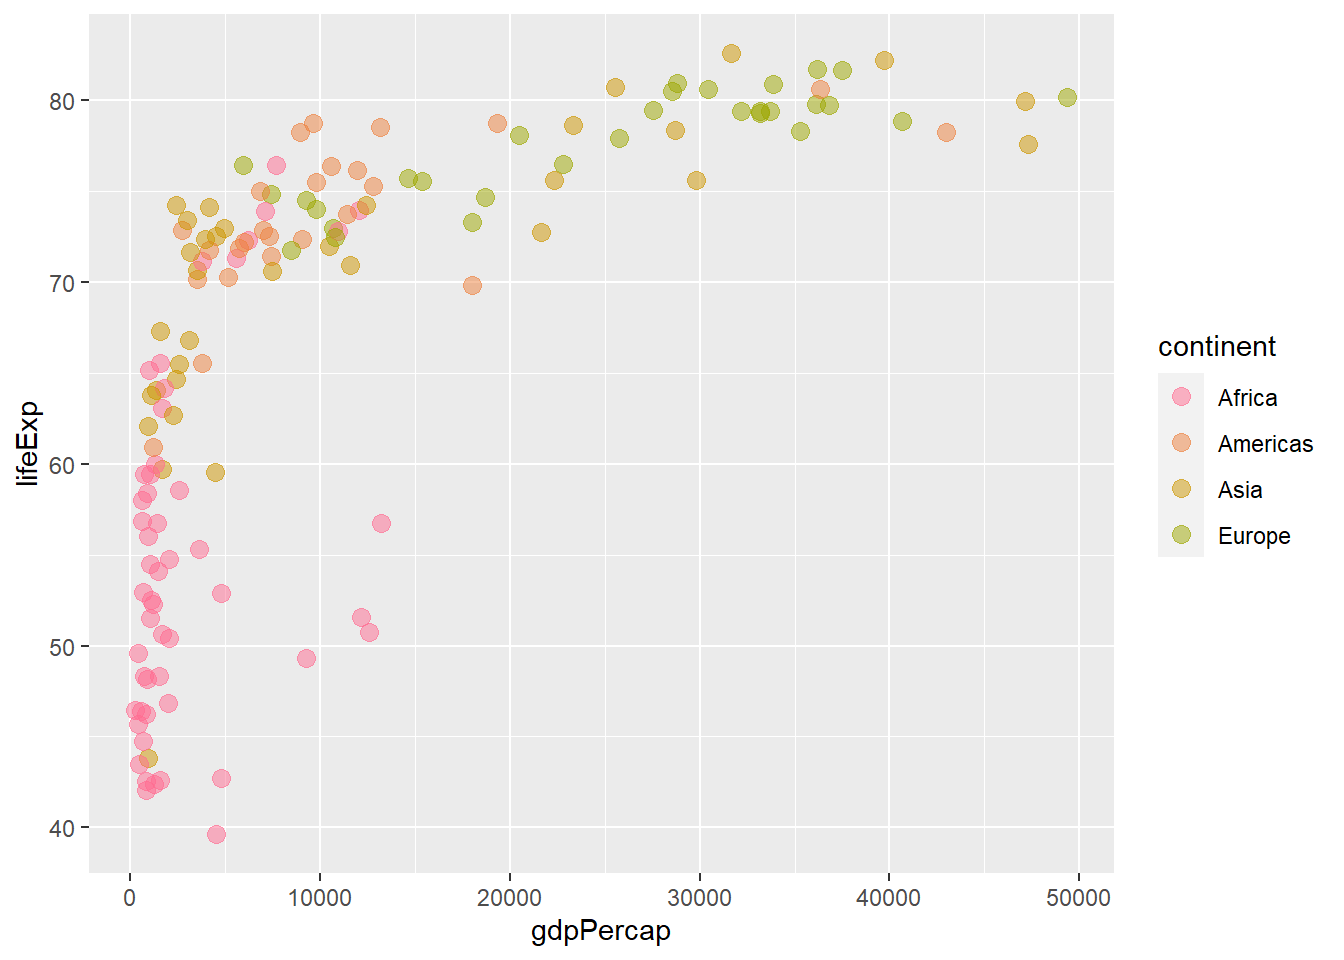
\includegraphics{05-ggplot2_files/figure-latex/unnamed-chunk-15-2.pdf}

\hypertarget{grey-colours}{%
\subsection{Grey colours}\label{grey-colours}}

The function \texttt{scale\_colour\_grey()} defines grey colours for discrete variables.

\begin{Shaded}
\begin{Highlighting}[]
\FunctionTok{ggplot}\NormalTok{(gapminder\_2007) }\SpecialCharTok{+} 
  \FunctionTok{geom\_point}\NormalTok{(}\FunctionTok{aes}\NormalTok{(}\AttributeTok{y =}\NormalTok{ lifeExp, }\AttributeTok{x =}\NormalTok{ gdpPercap, }\AttributeTok{colour =}\NormalTok{ continent), }\AttributeTok{size =} \DecValTok{3}\NormalTok{, }
             \AttributeTok{shape =} \DecValTok{19}\NormalTok{, }\AttributeTok{alpha =} \FloatTok{0.5}\NormalTok{) }\SpecialCharTok{+}
  \FunctionTok{scale\_colour\_grey}\NormalTok{()}
\end{Highlighting}
\end{Shaded}

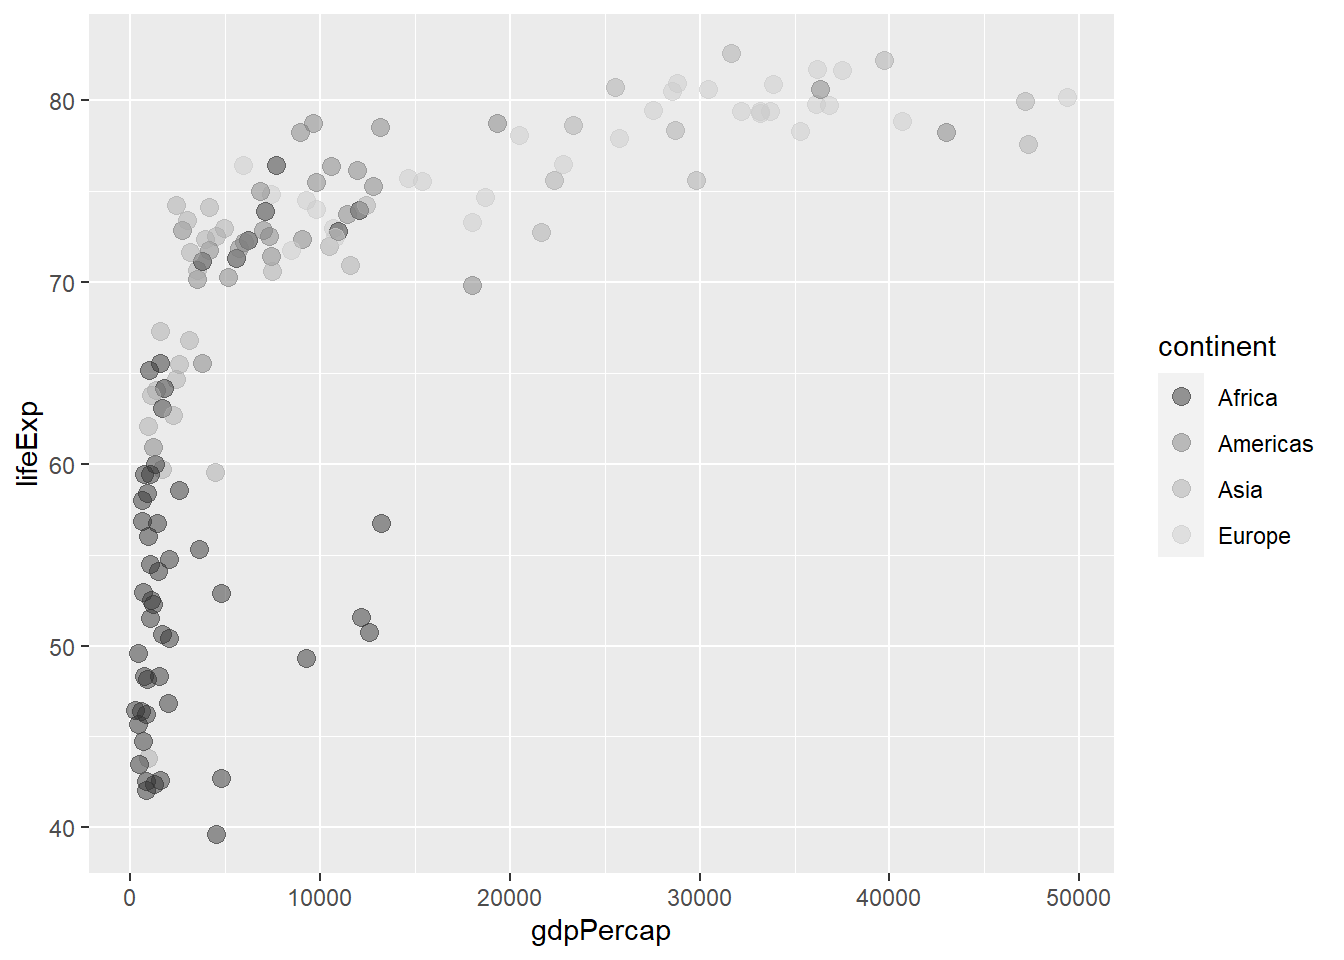
\includegraphics{05-ggplot2_files/figure-latex/unnamed-chunk-16-1.pdf}

\hypertarget{manually-specifying-colours}{%
\subsection{Manually specifying colours}\label{manually-specifying-colours}}

The functions \texttt{scale\_colour\_manual()} and \texttt{scale\_fill\_manual()} specify colour and fill, respectively.

\begin{Shaded}
\begin{Highlighting}[]
\FunctionTok{ggplot}\NormalTok{(gapminder\_2007) }\SpecialCharTok{+} 
  \FunctionTok{geom\_point}\NormalTok{(}\FunctionTok{aes}\NormalTok{(}\AttributeTok{y =}\NormalTok{ lifeExp, }\AttributeTok{x =}\NormalTok{ gdpPercap, }\AttributeTok{colour =}\NormalTok{ continent), }\AttributeTok{size =} \DecValTok{3}\NormalTok{, }
             \AttributeTok{shape =} \DecValTok{19}\NormalTok{, }\AttributeTok{alpha =} \FloatTok{0.5}\NormalTok{) }\SpecialCharTok{+}
  \FunctionTok{scale\_colour\_manual}\NormalTok{(}\AttributeTok{values =} \FunctionTok{c}\NormalTok{(}\StringTok{\textquotesingle{}lightblue\textquotesingle{}}\NormalTok{, }\StringTok{\textquotesingle{}lightgreen\textquotesingle{}}\NormalTok{, }\StringTok{\textquotesingle{}purple\textquotesingle{}}\NormalTok{, }\StringTok{\textquotesingle{}orange\textquotesingle{}}\NormalTok{, }\StringTok{\textquotesingle{}pink\textquotesingle{}}\NormalTok{))}
\end{Highlighting}
\end{Shaded}

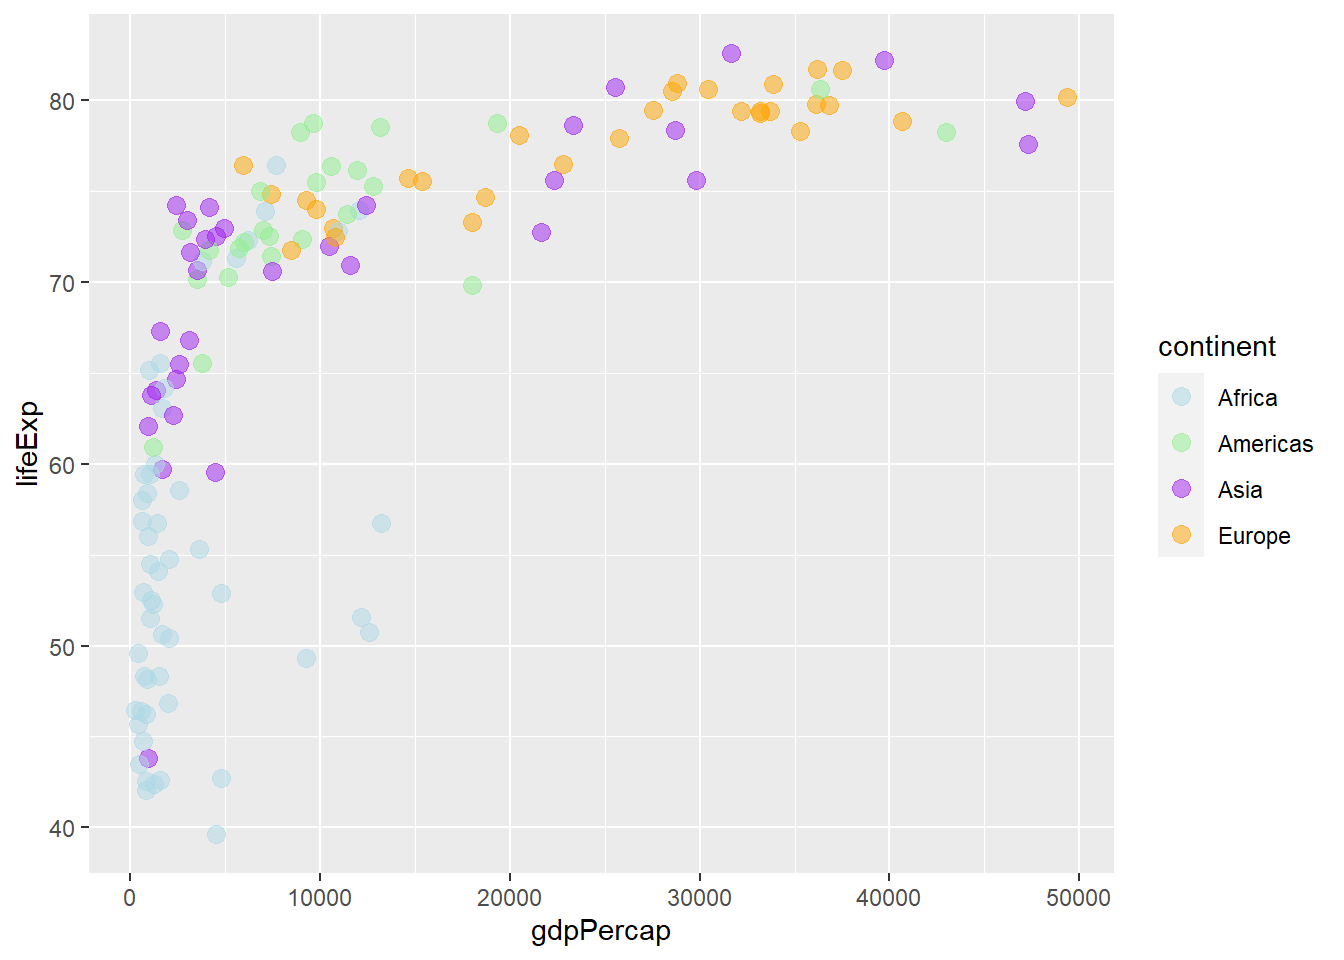
\includegraphics{05-ggplot2_files/figure-latex/unnamed-chunk-17-1.pdf}

\hypertarget{mapping-colours-by-continuous-variables}{%
\subsection{Mapping colours by continuous variables}\label{mapping-colours-by-continuous-variables}}

As with sizes, colours are mapped by assigning a continuous variable to them and placing them within \texttt{aes()}.

\begin{Shaded}
\begin{Highlighting}[]
\CommentTok{\# colour by pop}
\FunctionTok{ggplot}\NormalTok{(gapminder\_2007) }\SpecialCharTok{+} 
  \FunctionTok{geom\_point}\NormalTok{(}\FunctionTok{aes}\NormalTok{(}\AttributeTok{y =}\NormalTok{ lifeExp, }\AttributeTok{x =}\NormalTok{ gdpPercap, }\AttributeTok{size =}\NormalTok{ pop, }\AttributeTok{col =}\NormalTok{ pop), }\AttributeTok{shape =} \DecValTok{19}\NormalTok{) }\SpecialCharTok{+}
  \FunctionTok{scale\_radius}\NormalTok{(}\AttributeTok{range =} \FunctionTok{c}\NormalTok{(}\DecValTok{1}\NormalTok{, }\DecValTok{24}\NormalTok{))}
\end{Highlighting}
\end{Shaded}

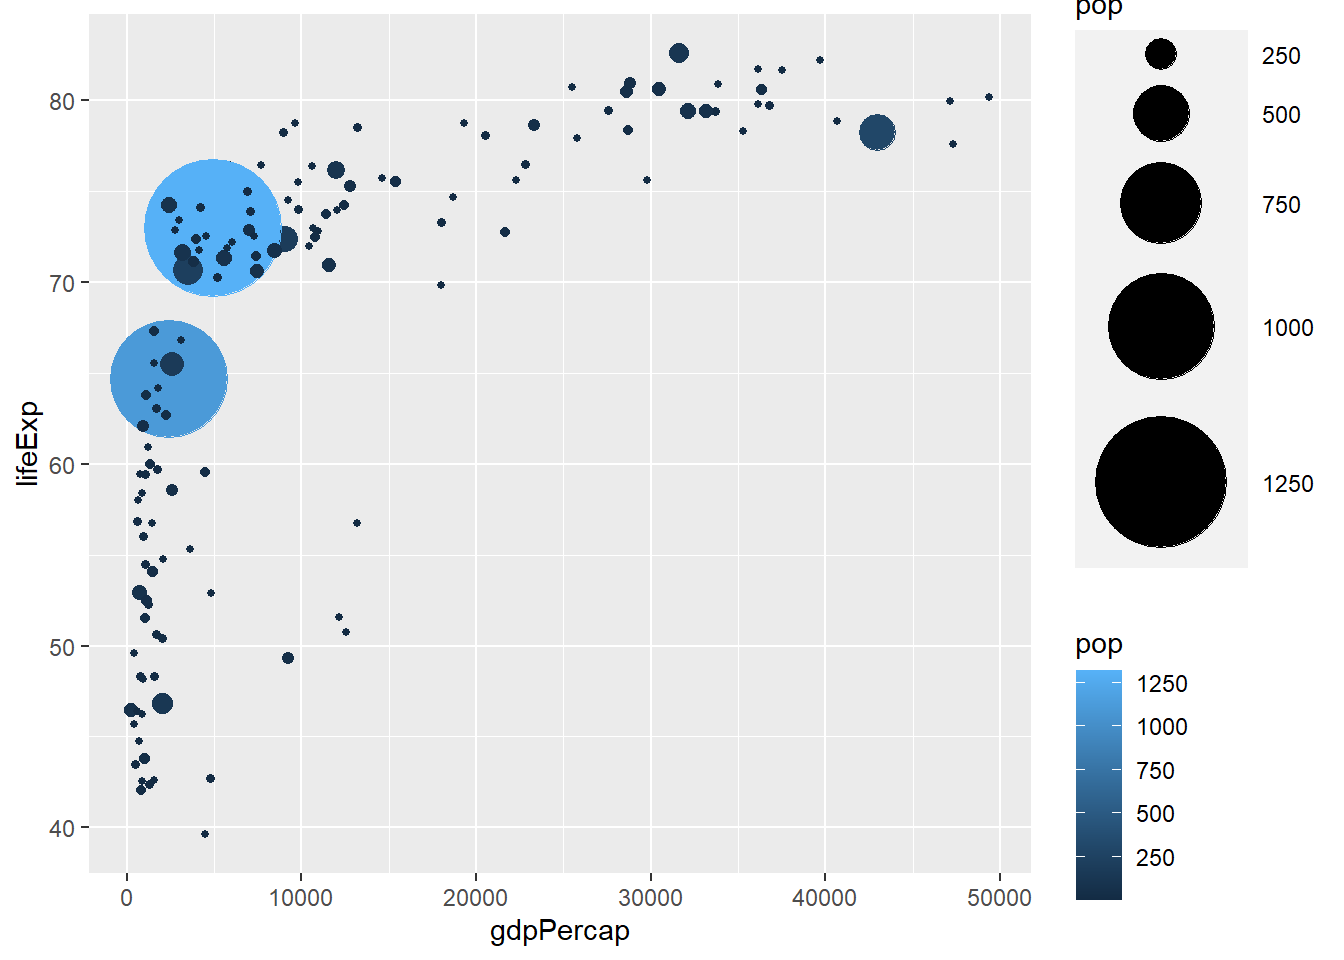
\includegraphics{05-ggplot2_files/figure-latex/unnamed-chunk-18-1.pdf}

\begin{Shaded}
\begin{Highlighting}[]
\CommentTok{\# reversing colour with desc()}
\FunctionTok{ggplot}\NormalTok{(gapminder\_2007) }\SpecialCharTok{+} 
  \FunctionTok{geom\_point}\NormalTok{(}\FunctionTok{aes}\NormalTok{(}\AttributeTok{y =}\NormalTok{ lifeExp, }\AttributeTok{x =}\NormalTok{ gdpPercap, }\AttributeTok{size =}\NormalTok{ pop, }\AttributeTok{colour =} \FunctionTok{desc}\NormalTok{(pop)), }\AttributeTok{shape =} \DecValTok{19}\NormalTok{) }\SpecialCharTok{+}
  \FunctionTok{scale\_radius}\NormalTok{(}\AttributeTok{range =} \FunctionTok{c}\NormalTok{(}\DecValTok{1}\NormalTok{, }\DecValTok{24}\NormalTok{))}
\end{Highlighting}
\end{Shaded}

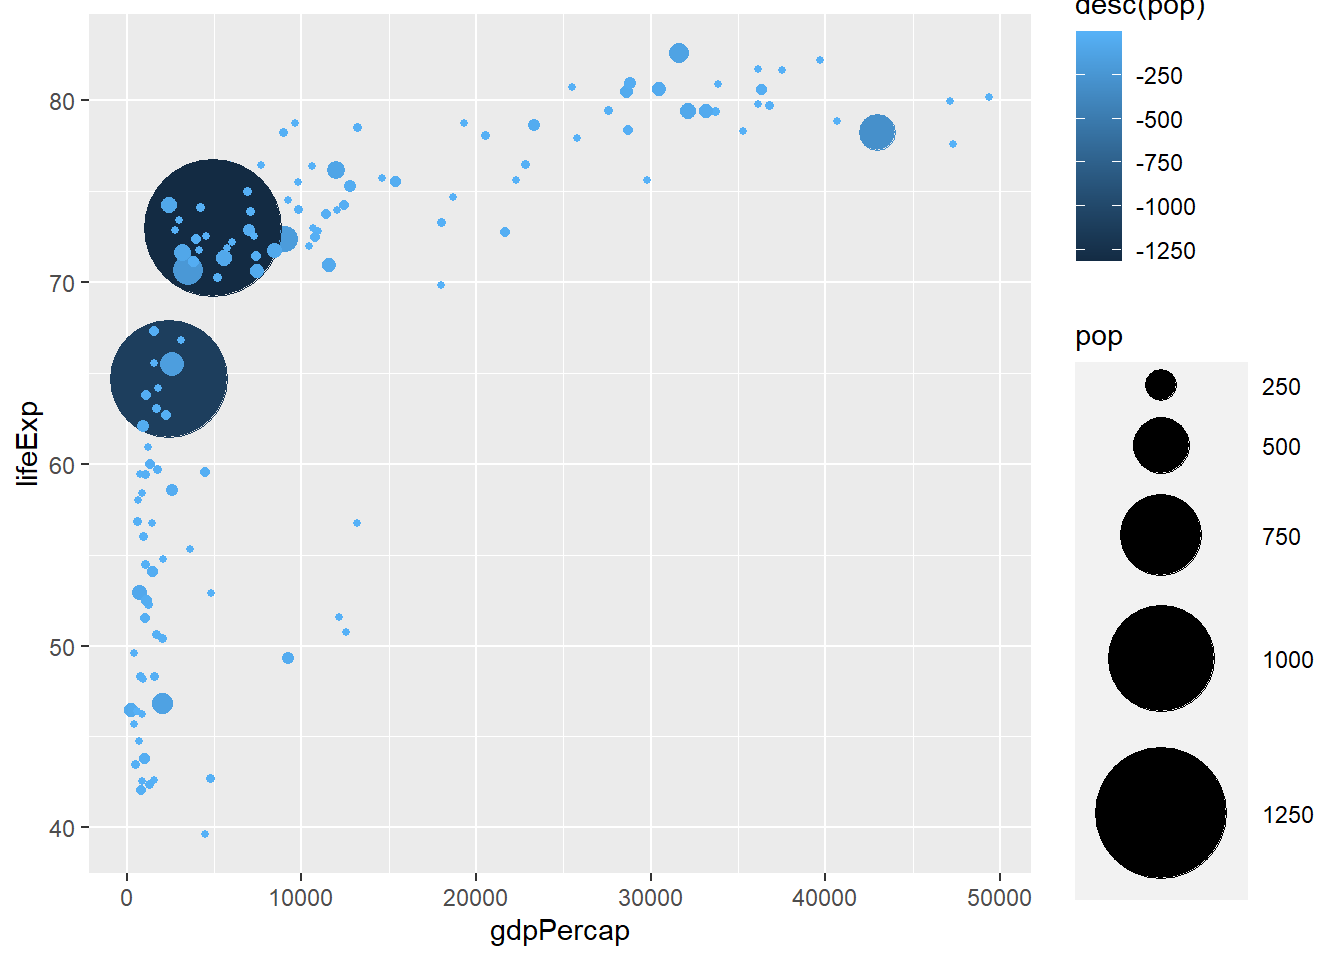
\includegraphics{05-ggplot2_files/figure-latex/unnamed-chunk-18-2.pdf}

\hypertarget{manually-defining-colours}{%
\subsection{Manually defining colours}\label{manually-defining-colours}}

The functions:

scale\_colour\_gradient() and scale\_fill\_gradient() defines a two-colour gradient
scale\_colour\_gradient2() and scale\_fill\_gradient2() defines a three-colour gradient (low-mid-high)
scale\_colour\_gradientn() and scale\_fill\_gradientn() defines a more then three colour gradient

\begin{Shaded}
\begin{Highlighting}[]
\CommentTok{\# two colour gradient}
\FunctionTok{ggplot}\NormalTok{(gapminder\_2007) }\SpecialCharTok{+} 
  \FunctionTok{geom\_point}\NormalTok{(}\FunctionTok{aes}\NormalTok{(}\AttributeTok{y =}\NormalTok{ lifeExp, }\AttributeTok{x =}\NormalTok{ gdpPercap, }\AttributeTok{size =}\NormalTok{ pop, }\AttributeTok{col =} \FunctionTok{desc}\NormalTok{(}\FunctionTok{log}\NormalTok{(pop))), }
           \AttributeTok{shape =} \DecValTok{19}\NormalTok{, }\AttributeTok{alpha =} \FloatTok{0.8}\NormalTok{) }\SpecialCharTok{+}
  \FunctionTok{scale\_radius}\NormalTok{(}\AttributeTok{range =} \FunctionTok{c}\NormalTok{(}\DecValTok{1}\NormalTok{, }\DecValTok{24}\NormalTok{)) }\SpecialCharTok{+}
  \FunctionTok{scale\_colour\_gradient}\NormalTok{(}\AttributeTok{low =} \StringTok{\textquotesingle{}lightgreen\textquotesingle{}}\NormalTok{, }\AttributeTok{high =} \StringTok{\textquotesingle{}darkgreen\textquotesingle{}}\NormalTok{)}
\end{Highlighting}
\end{Shaded}

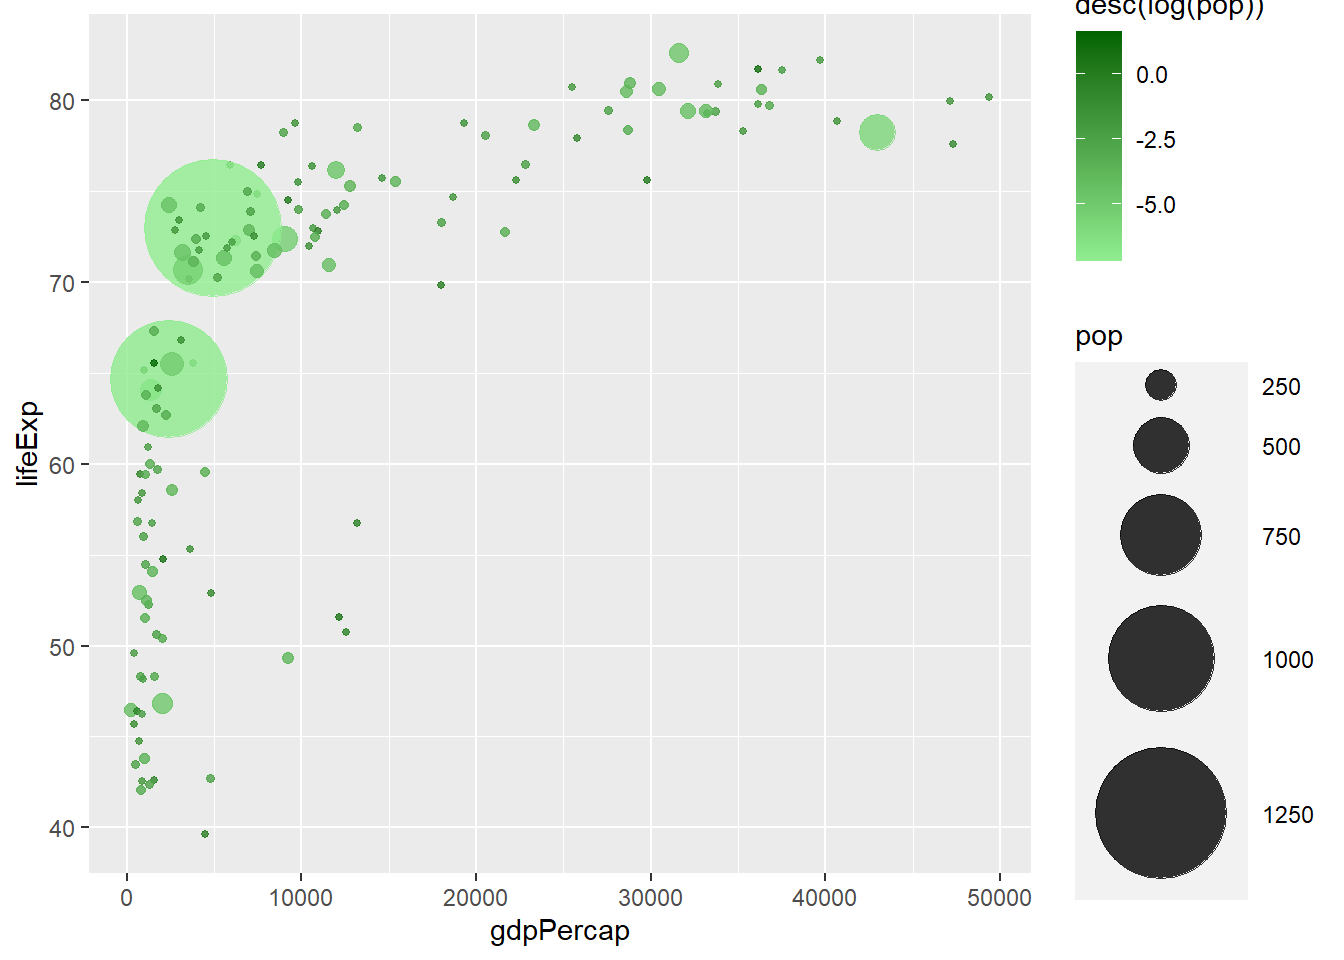
\includegraphics{05-ggplot2_files/figure-latex/unnamed-chunk-19-1.pdf}

\begin{Shaded}
\begin{Highlighting}[]
\CommentTok{\# three colour gradient}
\FunctionTok{ggplot}\NormalTok{(gapminder\_2007) }\SpecialCharTok{+} 
  \FunctionTok{geom\_point}\NormalTok{(}\FunctionTok{aes}\NormalTok{(}\AttributeTok{y =}\NormalTok{ lifeExp, }\AttributeTok{x =}\NormalTok{ gdpPercap, }\AttributeTok{size =}\NormalTok{ pop, }\AttributeTok{col =}\NormalTok{ pop), }
           \AttributeTok{shape =} \DecValTok{19}\NormalTok{, }\AttributeTok{alpha =} \FloatTok{0.8}\NormalTok{) }\SpecialCharTok{+}
  \FunctionTok{scale\_radius}\NormalTok{(}\AttributeTok{range =} \FunctionTok{c}\NormalTok{(}\DecValTok{1}\NormalTok{, }\DecValTok{24}\NormalTok{)) }\SpecialCharTok{+}
  \FunctionTok{scale\_colour\_gradient2}\NormalTok{(}\AttributeTok{low =} \StringTok{\textquotesingle{}blue\textquotesingle{}}\NormalTok{, }\AttributeTok{mid =} \StringTok{\textquotesingle{}red\textquotesingle{}}\NormalTok{, }\AttributeTok{high =} \StringTok{\textquotesingle{}green\textquotesingle{}}\NormalTok{, }
                         \AttributeTok{midpoint =} \FunctionTok{mean}\NormalTok{(gapminder\_2007}\SpecialCharTok{$}\NormalTok{pop))}
\end{Highlighting}
\end{Shaded}

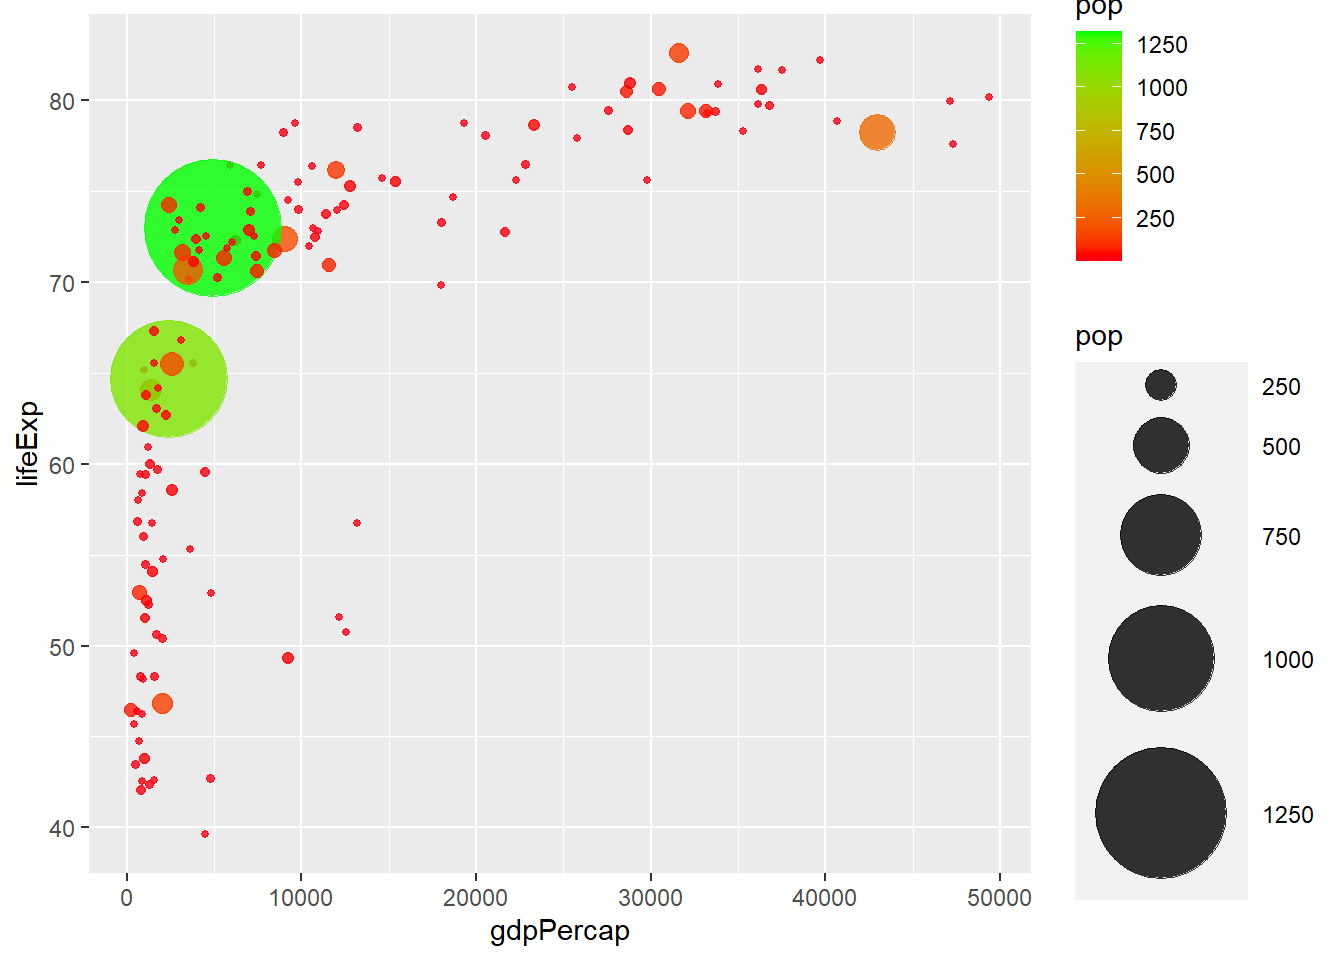
\includegraphics{05-ggplot2_files/figure-latex/unnamed-chunk-19-2.pdf}

\begin{Shaded}
\begin{Highlighting}[]
\CommentTok{\# five colour gradient}
\FunctionTok{ggplot}\NormalTok{(gapminder\_2007) }\SpecialCharTok{+} 
  \FunctionTok{geom\_point}\NormalTok{(}\FunctionTok{aes}\NormalTok{(}\AttributeTok{y =}\NormalTok{ lifeExp, }\AttributeTok{x =}\NormalTok{ gdpPercap, }\AttributeTok{size =}\NormalTok{ pop, }\AttributeTok{col =}\NormalTok{ pop), }\AttributeTok{shape =} \DecValTok{19}\NormalTok{) }\SpecialCharTok{+}
  \FunctionTok{scale\_radius}\NormalTok{(}\AttributeTok{range =} \FunctionTok{c}\NormalTok{(}\DecValTok{1}\NormalTok{, }\DecValTok{24}\NormalTok{)) }\SpecialCharTok{+}
  \FunctionTok{scale\_colour\_gradientn}\NormalTok{(}\AttributeTok{colors =} \FunctionTok{c}\NormalTok{(}\StringTok{\textquotesingle{}lightblue\textquotesingle{}}\NormalTok{, }\StringTok{\textquotesingle{}lightgreen\textquotesingle{}}\NormalTok{, }\StringTok{\textquotesingle{}purple\textquotesingle{}}\NormalTok{, }\StringTok{\textquotesingle{}orange\textquotesingle{}}\NormalTok{, }\StringTok{\textquotesingle{}pink\textquotesingle{}}\NormalTok{))}
\end{Highlighting}
\end{Shaded}

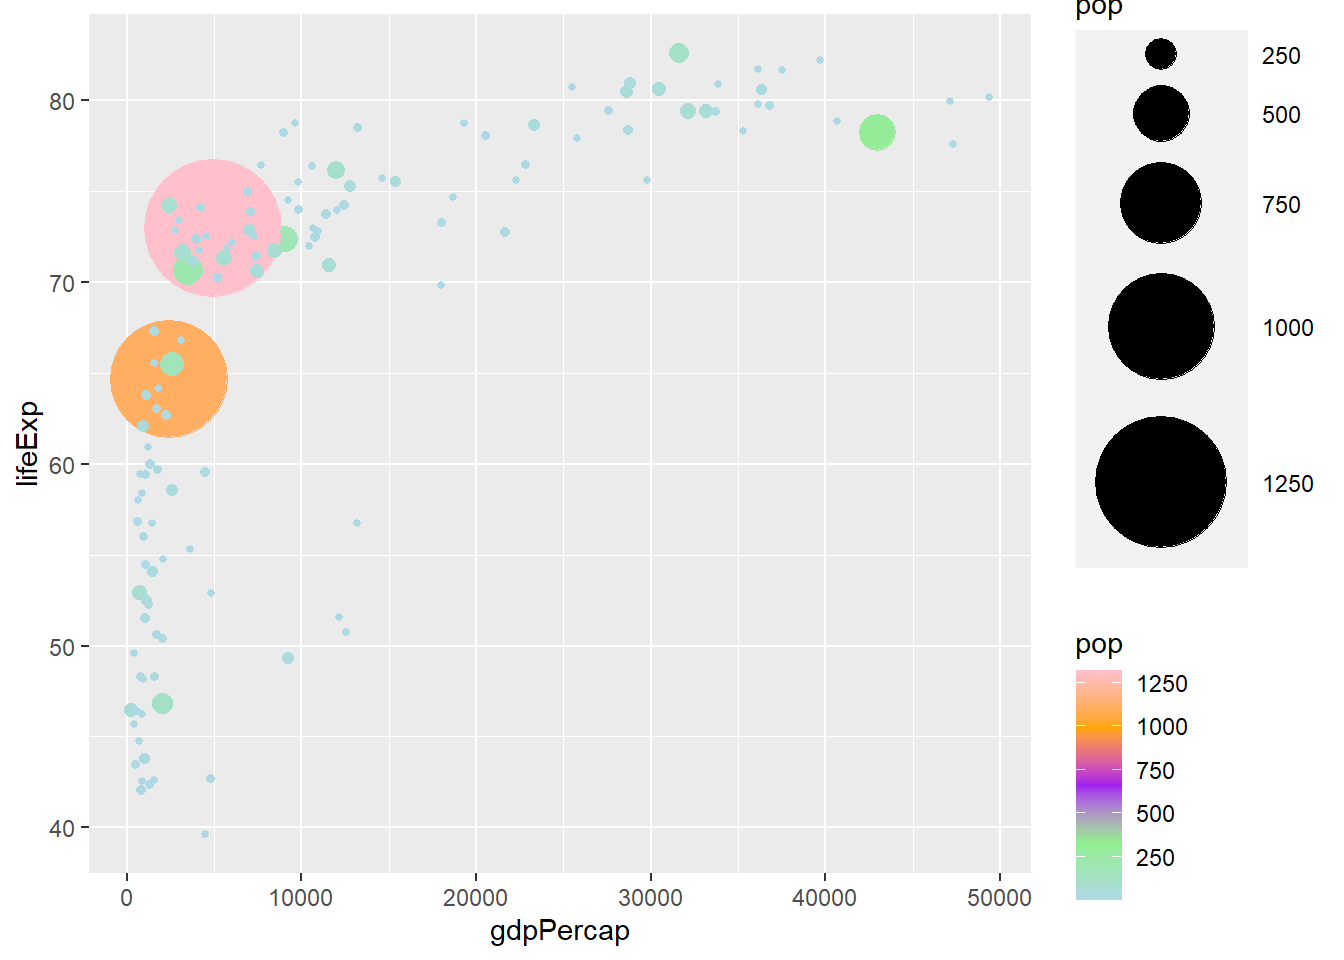
\includegraphics{05-ggplot2_files/figure-latex/unnamed-chunk-19-3.pdf}

\hypertarget{colour-palettes}{%
\section{Colour palettes}\label{colour-palettes}}

\hypertarget{rcolorbrewer}{%
\subsection{rcolorbrewer}\label{rcolorbrewer}}

RcolorBrewer is R's implementation of ColorBrewer. It classifies colours into three board classes:

seq (sequential): suited for data which has an order, progressing from low to high
div (diverging): suited for data with two extremes, one for positive and the other for negative values
qual (qualitative): suited for data which colour bears no meaning. (nominal and categorical data)

\begin{Shaded}
\begin{Highlighting}[]
\FunctionTok{library}\NormalTok{(RColorBrewer)}
\CommentTok{\# displays all the various palettes in RcolorBrewer}
\FunctionTok{display.brewer.all}\NormalTok{()}
\end{Highlighting}
\end{Shaded}

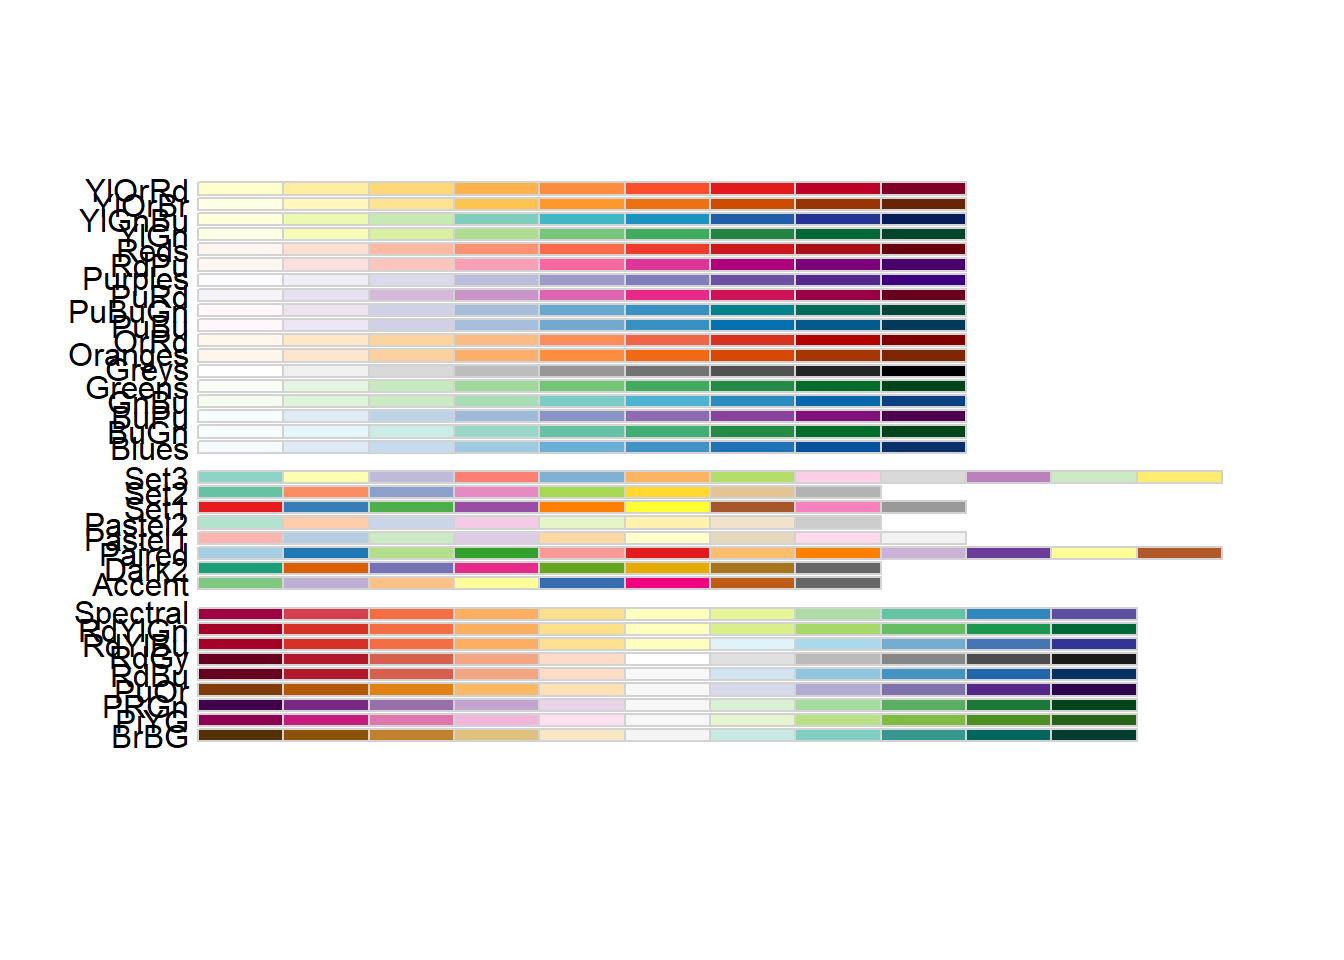
\includegraphics{05-ggplot2_files/figure-latex/unnamed-chunk-20-1.pdf}

\begin{Shaded}
\begin{Highlighting}[]


\CommentTok{\# display sequential colours}
\FunctionTok{display.brewer.all}\NormalTok{(}\AttributeTok{type =} \StringTok{"seq"}\NormalTok{)}
\end{Highlighting}
\end{Shaded}

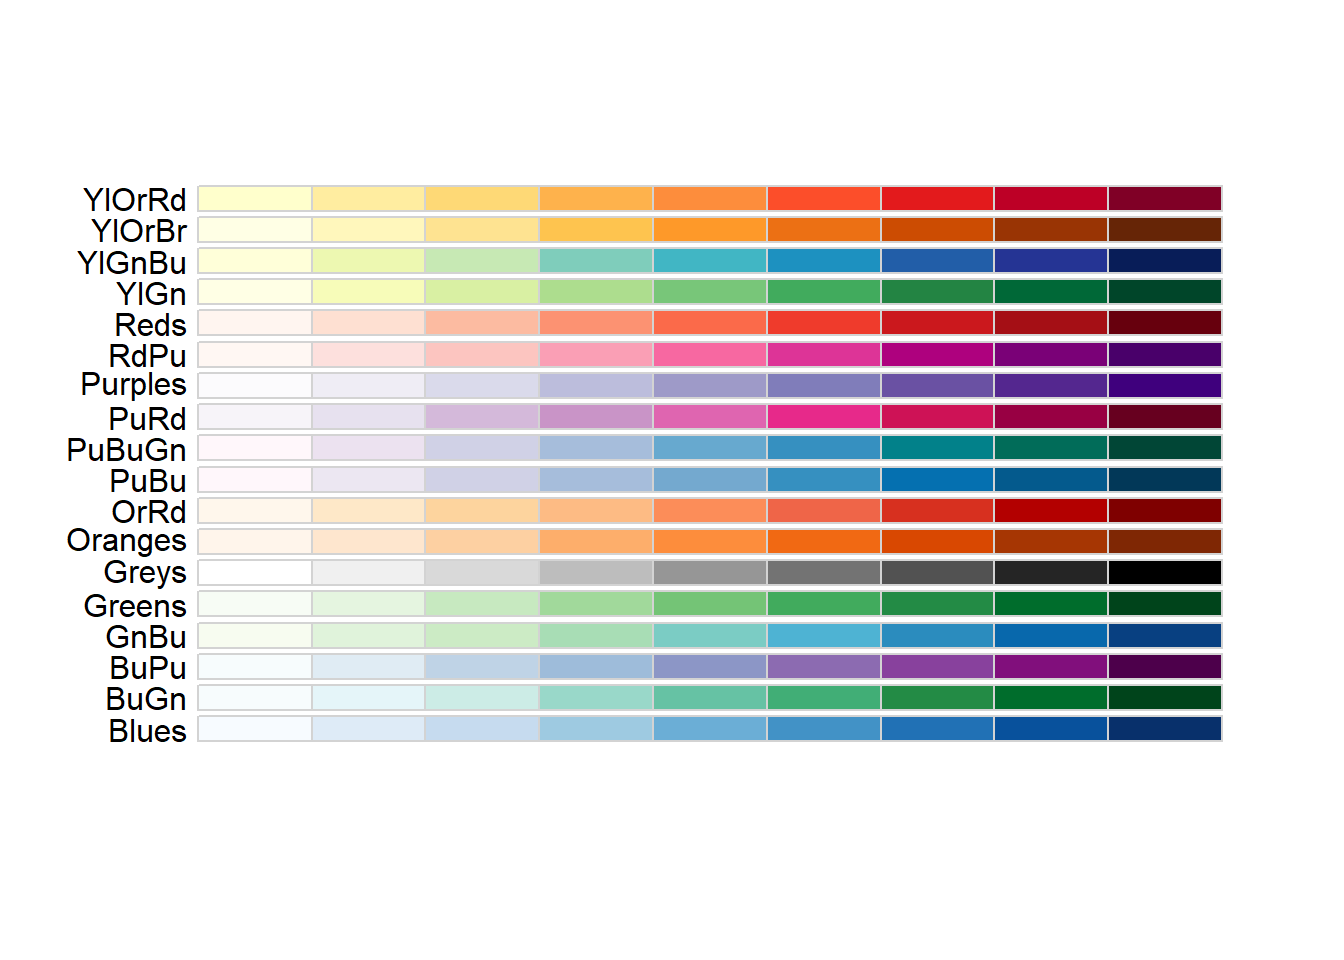
\includegraphics{05-ggplot2_files/figure-latex/unnamed-chunk-20-2.pdf}

\begin{Shaded}
\begin{Highlighting}[]


\CommentTok{\# display diverging colours}
\FunctionTok{display.brewer.all}\NormalTok{(}\AttributeTok{type =} \StringTok{"div"}\NormalTok{)}
\end{Highlighting}
\end{Shaded}

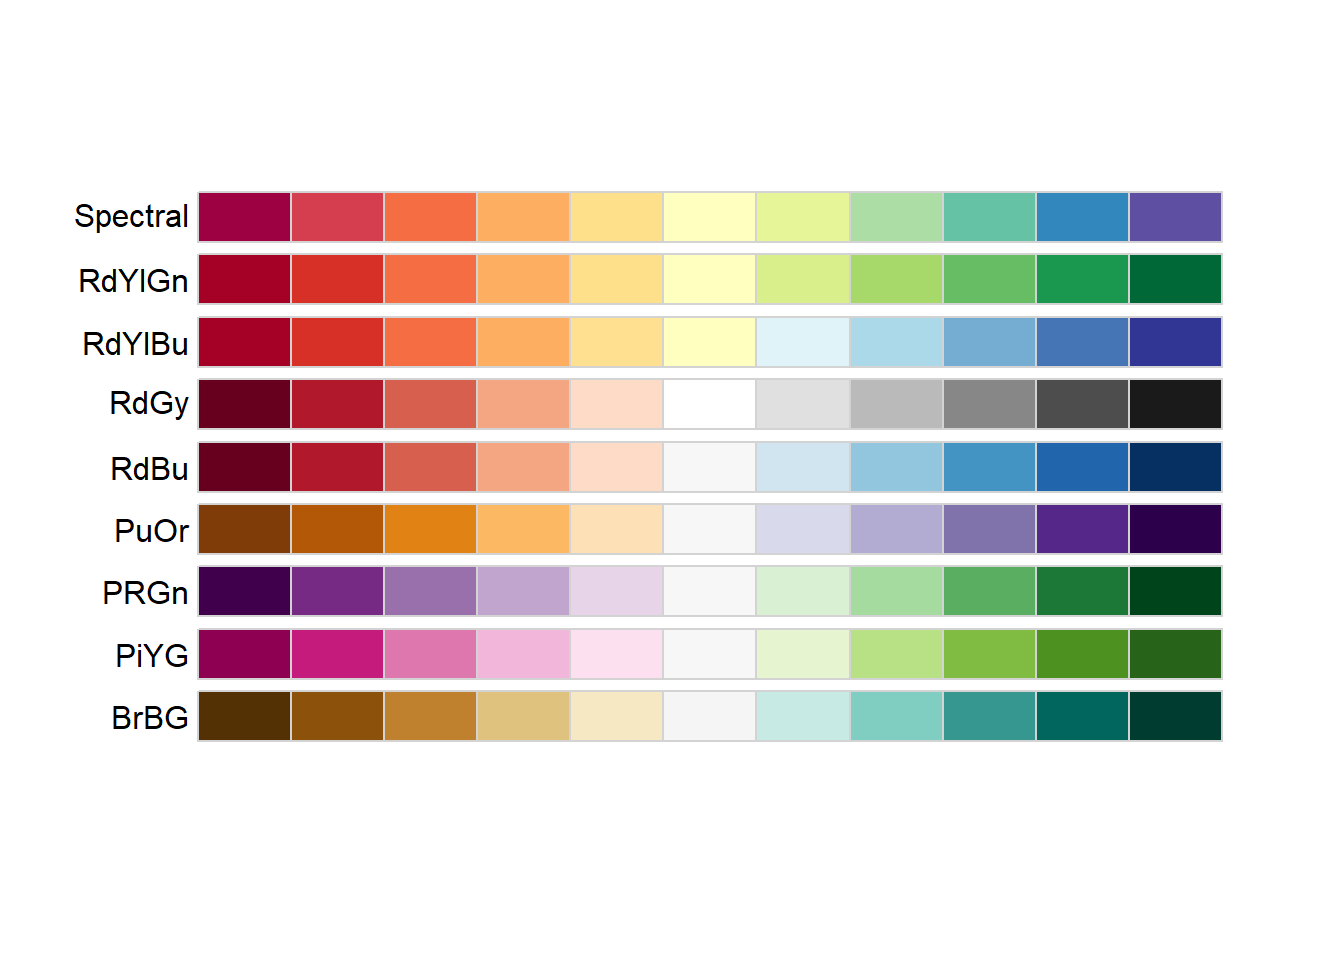
\includegraphics{05-ggplot2_files/figure-latex/unnamed-chunk-20-3.pdf}

\begin{Shaded}
\begin{Highlighting}[]


\CommentTok{\# display qualitative colours}
\FunctionTok{display.brewer.all}\NormalTok{(}\AttributeTok{type =} \StringTok{"qual"}\NormalTok{)}
\end{Highlighting}
\end{Shaded}

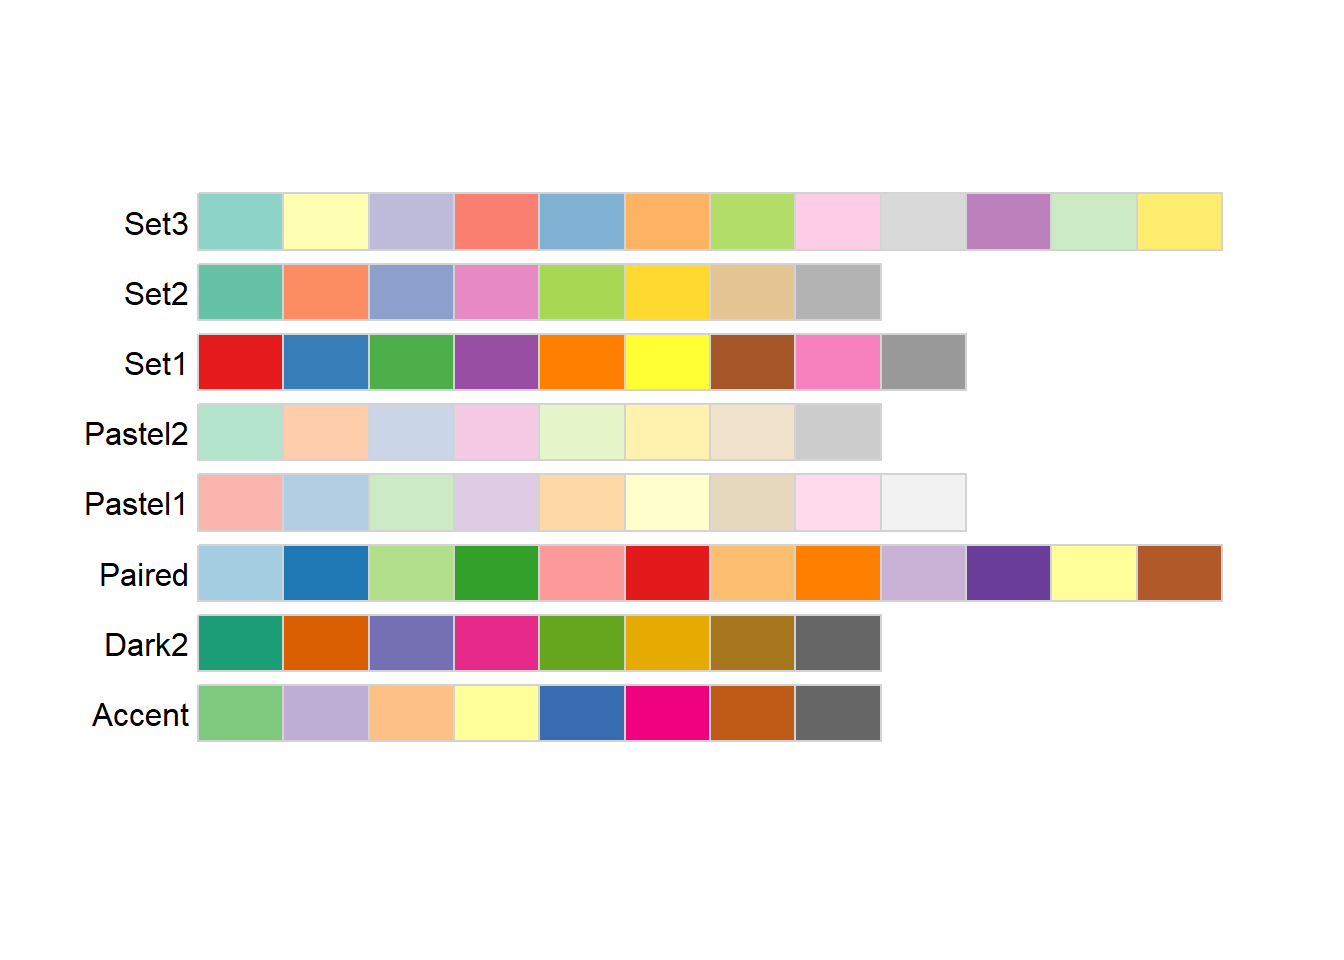
\includegraphics{05-ggplot2_files/figure-latex/unnamed-chunk-20-4.pdf}

\begin{Shaded}
\begin{Highlighting}[]


\CommentTok{\# displaying a particular colour palette}
\FunctionTok{display.brewer.pal}\NormalTok{(}\AttributeTok{n =} \DecValTok{8}\NormalTok{, }\AttributeTok{name =} \StringTok{\textquotesingle{}Dark2\textquotesingle{}}\NormalTok{)}
\end{Highlighting}
\end{Shaded}

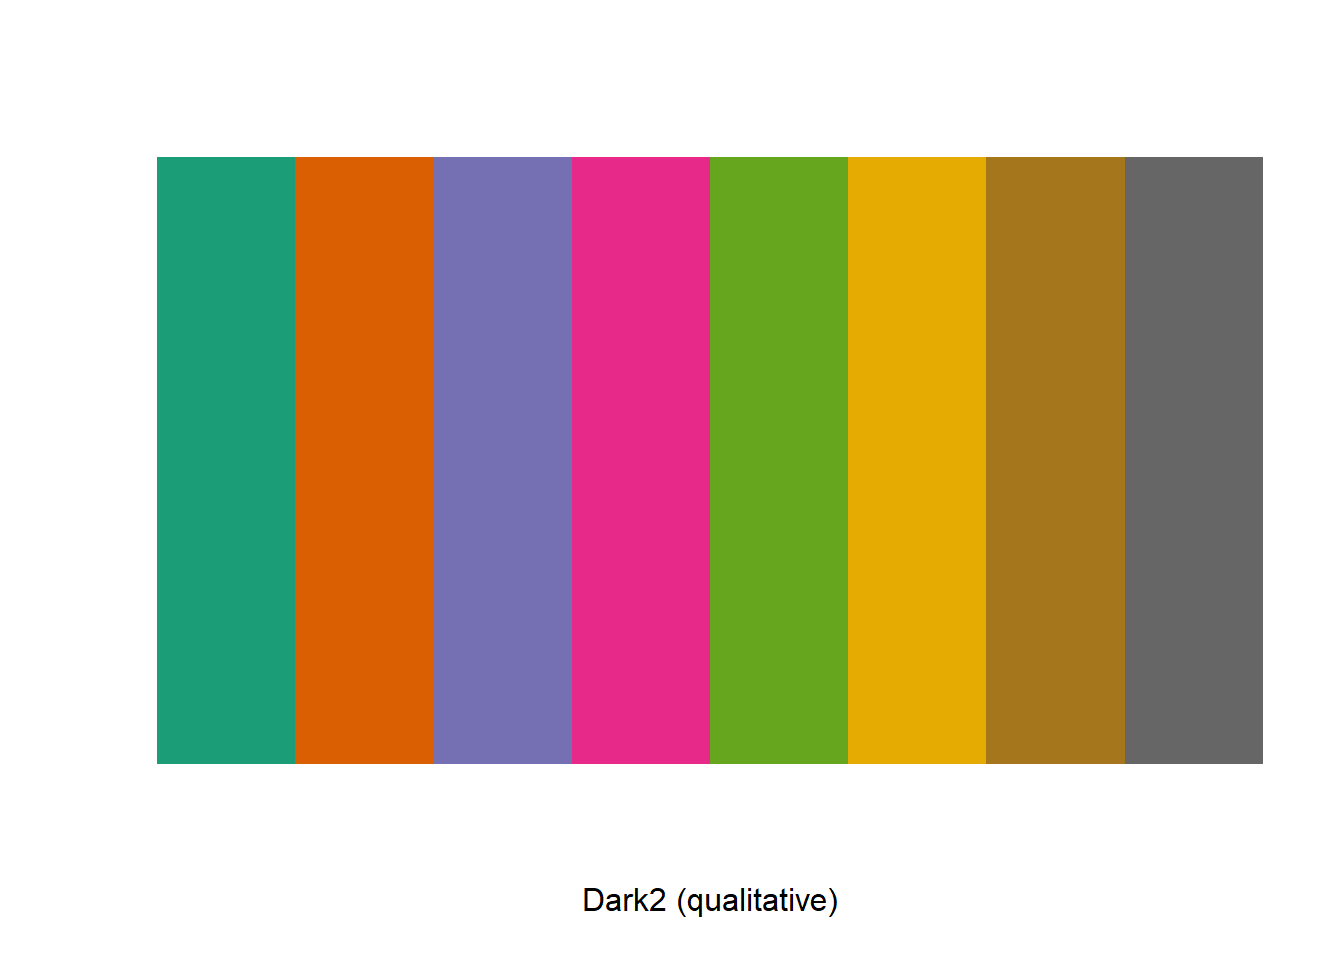
\includegraphics{05-ggplot2_files/figure-latex/unnamed-chunk-20-5.pdf}

The functions \texttt{scale\_colour\_brewer()} and \texttt{scale\_fill\_brewer()} defines colour scale for discrete variables.

\begin{Shaded}
\begin{Highlighting}[]
\CommentTok{\# discrete variable}
\FunctionTok{ggplot}\NormalTok{(gapminder\_2007) }\SpecialCharTok{+} 
  \FunctionTok{geom\_point}\NormalTok{(}\FunctionTok{aes}\NormalTok{(}\AttributeTok{y =}\NormalTok{ lifeExp, }\AttributeTok{x =}\NormalTok{ gdpPercap, }\AttributeTok{colour =}\NormalTok{ continent), }\AttributeTok{size =} \DecValTok{3}\NormalTok{, }\AttributeTok{shape =} \DecValTok{19}\NormalTok{, }
             \AttributeTok{alpha =} \FloatTok{0.5}\NormalTok{) }\SpecialCharTok{+}
  \FunctionTok{scale\_colour\_brewer}\NormalTok{(}\AttributeTok{palette =} \StringTok{"Dark2"}\NormalTok{)}
\end{Highlighting}
\end{Shaded}

\includegraphics{05-ggplot2_files/figure-latex/unnamed-chunk-21-1.pdf}

The argument direction reverses the order of the colours.

\begin{Shaded}
\begin{Highlighting}[]
\CommentTok{\# reversing colours with direction}
\FunctionTok{ggplot}\NormalTok{(gapminder\_2007) }\SpecialCharTok{+} 
  \FunctionTok{geom\_point}\NormalTok{(}\FunctionTok{aes}\NormalTok{(}\AttributeTok{y =}\NormalTok{ lifeExp, }\AttributeTok{x =}\NormalTok{ gdpPercap, }\AttributeTok{colour =}\NormalTok{ continent), }\AttributeTok{size =} \DecValTok{3}\NormalTok{, }\AttributeTok{shape =} \DecValTok{19}\NormalTok{, }
             \AttributeTok{alpha =} \FloatTok{0.5}\NormalTok{) }\SpecialCharTok{+}
  \FunctionTok{scale\_colour\_brewer}\NormalTok{(}\AttributeTok{palette =} \StringTok{"Dark2"}\NormalTok{, }\AttributeTok{direction =} \SpecialCharTok{{-}}\DecValTok{1}\NormalTok{)}
\end{Highlighting}
\end{Shaded}

\includegraphics{05-ggplot2_files/figure-latex/unnamed-chunk-22-1.pdf}

The type of palette is specified by the argument type.

\begin{Shaded}
\begin{Highlighting}[]
\CommentTok{\# specifying palette class}
\FunctionTok{ggplot}\NormalTok{(gapminder\_2007) }\SpecialCharTok{+} 
  \FunctionTok{geom\_point}\NormalTok{(}\FunctionTok{aes}\NormalTok{(}\AttributeTok{y =}\NormalTok{ lifeExp, }\AttributeTok{x =}\NormalTok{ gdpPercap, }\AttributeTok{colour =}\NormalTok{ continent), }\AttributeTok{size =} \DecValTok{3}\NormalTok{, }\AttributeTok{shape =} \DecValTok{19}\NormalTok{, }
             \AttributeTok{alpha =} \FloatTok{0.5}\NormalTok{) }\SpecialCharTok{+}
  \FunctionTok{scale\_colour\_brewer}\NormalTok{(}\AttributeTok{type =} \StringTok{\textquotesingle{}qual\textquotesingle{}}\NormalTok{, }\AttributeTok{palette =} \DecValTok{1}\NormalTok{)}
\end{Highlighting}
\end{Shaded}

\includegraphics{05-ggplot2_files/figure-latex/unnamed-chunk-23-1.pdf}

\begin{Shaded}
\begin{Highlighting}[]
\CommentTok{\# specifying palette class}
\FunctionTok{ggplot}\NormalTok{(gapminder\_2007) }\SpecialCharTok{+} 
  \FunctionTok{geom\_point}\NormalTok{(}\FunctionTok{aes}\NormalTok{(}\AttributeTok{y =}\NormalTok{ lifeExp, }\AttributeTok{x =}\NormalTok{ gdpPercap, }\AttributeTok{colour =}\NormalTok{ continent), }\AttributeTok{size =} \DecValTok{3}\NormalTok{, }\AttributeTok{shape =} \DecValTok{19}\NormalTok{, }
             \AttributeTok{alpha =} \FloatTok{0.5}\NormalTok{) }\SpecialCharTok{+}
  \FunctionTok{scale\_colour\_brewer}\NormalTok{(}\AttributeTok{type =} \StringTok{\textquotesingle{}seq\textquotesingle{}}\NormalTok{, }\AttributeTok{palette =} \DecValTok{3}\NormalTok{)}
\end{Highlighting}
\end{Shaded}

\includegraphics{05-ggplot2_files/figure-latex/unnamed-chunk-23-2.pdf}

The functions \texttt{scale\_colour\_distiller()} and \texttt{scale\_fill\_distiller()} defines colour scale for continuous variables.

\begin{Shaded}
\begin{Highlighting}[]
\CommentTok{\# continuous variable}
\FunctionTok{ggplot}\NormalTok{(gapminder\_2007) }\SpecialCharTok{+} 
  \FunctionTok{geom\_point}\NormalTok{(}\FunctionTok{aes}\NormalTok{(}\AttributeTok{y =}\NormalTok{ lifeExp, }\AttributeTok{x =}\NormalTok{ gdpPercap, }\AttributeTok{size =}\NormalTok{ pop, }\AttributeTok{col =} \FunctionTok{log}\NormalTok{(pop)), }\AttributeTok{shape =} \DecValTok{19}\NormalTok{) }\SpecialCharTok{+}
  \FunctionTok{scale\_radius}\NormalTok{(}\AttributeTok{range =} \FunctionTok{c}\NormalTok{(}\DecValTok{1}\NormalTok{, }\DecValTok{24}\NormalTok{)) }\SpecialCharTok{+}
  \FunctionTok{scale\_colour\_distiller}\NormalTok{(}\AttributeTok{palette =} \StringTok{\textquotesingle{}Blues\textquotesingle{}}\NormalTok{)}
\end{Highlighting}
\end{Shaded}

\includegraphics{05-ggplot2_files/figure-latex/unnamed-chunk-24-1.pdf}

\begin{Shaded}
\begin{Highlighting}[]
\CommentTok{\# continuous variable}
\FunctionTok{ggplot}\NormalTok{(gapminder\_2007) }\SpecialCharTok{+} 
  \FunctionTok{geom\_point}\NormalTok{(}\FunctionTok{aes}\NormalTok{(}\AttributeTok{y =}\NormalTok{ lifeExp, }\AttributeTok{x =}\NormalTok{ gdpPercap, }\AttributeTok{size =}\NormalTok{ pop, }\AttributeTok{col =} \FunctionTok{log}\NormalTok{(pop)), }\AttributeTok{shape =} \DecValTok{19}\NormalTok{) }\SpecialCharTok{+}
  \FunctionTok{scale\_radius}\NormalTok{(}\AttributeTok{range =} \FunctionTok{c}\NormalTok{(}\DecValTok{1}\NormalTok{, }\DecValTok{24}\NormalTok{)) }\SpecialCharTok{+}
  \FunctionTok{scale\_colour\_distiller}\NormalTok{(}\AttributeTok{palette =} \DecValTok{1}\NormalTok{, }\AttributeTok{direction =} \DecValTok{1}\NormalTok{)}
\end{Highlighting}
\end{Shaded}

\includegraphics{05-ggplot2_files/figure-latex/unnamed-chunk-24-2.pdf}

\hypertarget{the-viridis-color-palettes}{%
\subsection{The viridis color palettes}\label{the-viridis-color-palettes}}

The viridis package brings to R colour scales created by Stéfan van der Walt and Nathaniel Smith for the Python data visualization package matplotlib. viridis comes with the following colour palettes:

\begin{itemize}
\tightlist
\item
  Viridis (default)
\item
  magma
\item
  plasma
\item
  inferno
\end{itemize}

The functions \texttt{scale\_colour\_viridis()} and \texttt{scale\_fill\_viridis()} defines colour scale for both discrete and continuous variables, with \texttt{discrete\ =\ TRUE} indicating discrete while \texttt{discrete\ =\ FALSE} indicating continuous. To be more specific, use \texttt{scale\_colour\_viridis\_d()} for discrete and\texttt{scale\_colour\_viridis\_c()} for continuous.

\begin{Shaded}
\begin{Highlighting}[]
\FunctionTok{library}\NormalTok{(viridis)}
\CommentTok{\# discrete variable}
\FunctionTok{ggplot}\NormalTok{(gapminder\_2007) }\SpecialCharTok{+} 
  \FunctionTok{geom\_point}\NormalTok{(}\FunctionTok{aes}\NormalTok{(}\AttributeTok{y =}\NormalTok{ lifeExp, }\AttributeTok{x =}\NormalTok{ gdpPercap, }\AttributeTok{colour =}\NormalTok{ continent), }\AttributeTok{size =} \DecValTok{3}\NormalTok{, }
           \AttributeTok{shape =} \DecValTok{19}\NormalTok{, }\AttributeTok{alpha =} \FloatTok{0.8}\NormalTok{) }\SpecialCharTok{+}
  \FunctionTok{scale\_colour\_viridis}\NormalTok{(}\AttributeTok{discrete =} \ConstantTok{TRUE}\NormalTok{)}
\end{Highlighting}
\end{Shaded}

\includegraphics{05-ggplot2_files/figure-latex/unnamed-chunk-25-1.pdf}

\begin{Shaded}
\begin{Highlighting}[]
\CommentTok{\# discrete variable}
\FunctionTok{ggplot}\NormalTok{(gapminder\_2007) }\SpecialCharTok{+} 
  \FunctionTok{geom\_point}\NormalTok{(}\FunctionTok{aes}\NormalTok{(}\AttributeTok{y =}\NormalTok{ lifeExp, }\AttributeTok{x =}\NormalTok{ gdpPercap, }\AttributeTok{colour =}\NormalTok{ continent), }\AttributeTok{size =} \DecValTok{3}\NormalTok{, }
             \AttributeTok{shape =} \DecValTok{19}\NormalTok{, }\AttributeTok{alpha =} \FloatTok{0.8}\NormalTok{) }\SpecialCharTok{+}
  \FunctionTok{scale\_colour\_viridis\_d}\NormalTok{(}\AttributeTok{option =} \StringTok{\textquotesingle{}plasma\textquotesingle{}}\NormalTok{)}
\end{Highlighting}
\end{Shaded}

\includegraphics{05-ggplot2_files/figure-latex/unnamed-chunk-25-2.pdf}

\begin{Shaded}
\begin{Highlighting}[]

\CommentTok{\# continuous variable}
\FunctionTok{ggplot}\NormalTok{(gapminder\_2007) }\SpecialCharTok{+} 
  \FunctionTok{geom\_point}\NormalTok{(}\FunctionTok{aes}\NormalTok{(}\AttributeTok{y =}\NormalTok{ lifeExp, }\AttributeTok{x =}\NormalTok{ gdpPercap, }\AttributeTok{size =}\NormalTok{ pop, }\AttributeTok{col =} \FunctionTok{log}\NormalTok{(pop)), }\AttributeTok{shape =} \DecValTok{19}\NormalTok{) }\SpecialCharTok{+}
  \FunctionTok{scale\_radius}\NormalTok{(}\AttributeTok{range =} \FunctionTok{c}\NormalTok{(}\DecValTok{1}\NormalTok{, }\DecValTok{24}\NormalTok{)) }\SpecialCharTok{+}
  \FunctionTok{scale\_colour\_viridis}\NormalTok{()}
\end{Highlighting}
\end{Shaded}

\includegraphics{05-ggplot2_files/figure-latex/unnamed-chunk-25-3.pdf}

\begin{Shaded}
\begin{Highlighting}[]
\CommentTok{\# continuous variable}
\FunctionTok{ggplot}\NormalTok{(gapminder\_2007) }\SpecialCharTok{+} 
  \FunctionTok{geom\_point}\NormalTok{(}\FunctionTok{aes}\NormalTok{(}\AttributeTok{y =}\NormalTok{ lifeExp, }\AttributeTok{x =}\NormalTok{ gdpPercap, }\AttributeTok{size =}\NormalTok{ pop, }\AttributeTok{col =} \FunctionTok{log}\NormalTok{(pop)), }\AttributeTok{shape =} \DecValTok{19}\NormalTok{) }\SpecialCharTok{+}
  \FunctionTok{scale\_radius}\NormalTok{(}\AttributeTok{range =} \FunctionTok{c}\NormalTok{(}\DecValTok{1}\NormalTok{, }\DecValTok{24}\NormalTok{)) }\SpecialCharTok{+}
  \FunctionTok{scale\_colour\_viridis\_c}\NormalTok{(}\AttributeTok{option =} \StringTok{\textquotesingle{}inferno\textquotesingle{}}\NormalTok{, }\AttributeTok{direction =} \SpecialCharTok{{-}}\DecValTok{1}\NormalTok{, }\AttributeTok{alpha =} \FloatTok{0.5}\NormalTok{)}
\end{Highlighting}
\end{Shaded}

\includegraphics{05-ggplot2_files/figure-latex/unnamed-chunk-25-4.pdf}

\hypertarget{text}{%
\section{Text}\label{text}}

The function \texttt{geom\_text()} adds text to a plot.

\begin{Shaded}
\begin{Highlighting}[]
\FunctionTok{ggplot}\NormalTok{(}\AttributeTok{data =}\NormalTok{ gapminder\_2007, }\FunctionTok{aes}\NormalTok{(}\AttributeTok{y =}\NormalTok{ lifeExp, }\AttributeTok{x =}\NormalTok{ gdpPercap)) }\SpecialCharTok{+} 
  \FunctionTok{geom\_point}\NormalTok{(}\AttributeTok{alpha =} \FloatTok{0.5}\NormalTok{, }\AttributeTok{stroke =} \DecValTok{1}\NormalTok{, }\FunctionTok{aes}\NormalTok{(}\AttributeTok{size =}\NormalTok{ pop, }\AttributeTok{colour =}\NormalTok{ continent)) }\SpecialCharTok{+}
  \FunctionTok{scale\_size\_area}\NormalTok{(}\AttributeTok{max\_size =} \DecValTok{12}\NormalTok{) }\SpecialCharTok{+}
  \FunctionTok{geom\_text}\NormalTok{(}\FunctionTok{aes}\NormalTok{(}\AttributeTok{label =}\NormalTok{ country), }\AttributeTok{size =} \DecValTok{2}\NormalTok{, }\AttributeTok{alpha =} \FloatTok{0.5}\NormalTok{)}
\end{Highlighting}
\end{Shaded}

\includegraphics{05-ggplot2_files/figure-latex/unnamed-chunk-26-1.pdf}

\hypertarget{fitting-a-regression-line-to-a-plot}{%
\section{Fitting a regression line to a plot}\label{fitting-a-regression-line-to-a-plot}}

The function \texttt{geom\_smooth()} adds a regression line to a plot. We use the arguments:

method = lm for linear,
method = loess for loess and
se = FALSE to remove the confidence intervals.

\begin{Shaded}
\begin{Highlighting}[]
\CommentTok{\# adding a linear line}
\FunctionTok{ggplot}\NormalTok{(}\AttributeTok{data =}\NormalTok{ gapminder\_2007, }\FunctionTok{aes}\NormalTok{(}\AttributeTok{y =}\NormalTok{ lifeExp, }\AttributeTok{x =}\NormalTok{ gdpPercap)) }\SpecialCharTok{+} 
  \FunctionTok{geom\_point}\NormalTok{(}\AttributeTok{colour =} \StringTok{\textquotesingle{}red\textquotesingle{}}\NormalTok{, }\AttributeTok{size =} \DecValTok{3}\NormalTok{, }\AttributeTok{shape =} \DecValTok{19}\NormalTok{, }\AttributeTok{alpha =} \FloatTok{0.5}\NormalTok{, }\AttributeTok{stroke =} \DecValTok{1}\NormalTok{) }\SpecialCharTok{+}
  \FunctionTok{geom\_smooth}\NormalTok{(}\AttributeTok{method =}\NormalTok{ lm)}
\end{Highlighting}
\end{Shaded}

\includegraphics{05-ggplot2_files/figure-latex/unnamed-chunk-27-1.pdf}

\begin{Shaded}
\begin{Highlighting}[]
\CommentTok{\# changing to loess}
\FunctionTok{ggplot}\NormalTok{(}\AttributeTok{data =}\NormalTok{ gapminder\_2007, }\FunctionTok{aes}\NormalTok{(}\AttributeTok{y =}\NormalTok{ lifeExp, }\AttributeTok{x =}\NormalTok{ gdpPercap)) }\SpecialCharTok{+} 
  \FunctionTok{geom\_point}\NormalTok{(}\AttributeTok{colour =} \StringTok{\textquotesingle{}red\textquotesingle{}}\NormalTok{, }\AttributeTok{size =} \DecValTok{3}\NormalTok{, }\AttributeTok{shape =} \DecValTok{19}\NormalTok{, }\AttributeTok{alpha =} \FloatTok{0.5}\NormalTok{, }\AttributeTok{stroke =} \DecValTok{1}\NormalTok{) }\SpecialCharTok{+}
  \FunctionTok{geom\_smooth}\NormalTok{(}\AttributeTok{method =}\NormalTok{ loess)}
\end{Highlighting}
\end{Shaded}

\includegraphics{05-ggplot2_files/figure-latex/unnamed-chunk-27-2.pdf}

\begin{Shaded}
\begin{Highlighting}[]
\CommentTok{\# removing the confidence intervals}
\FunctionTok{ggplot}\NormalTok{(}\AttributeTok{data =}\NormalTok{ gapminder\_2007, }\FunctionTok{aes}\NormalTok{(}\AttributeTok{y =}\NormalTok{ lifeExp, }\AttributeTok{x =}\NormalTok{ gdpPercap)) }\SpecialCharTok{+} 
  \FunctionTok{geom\_point}\NormalTok{(}\AttributeTok{colour =} \StringTok{\textquotesingle{}red\textquotesingle{}}\NormalTok{, }\AttributeTok{size =} \DecValTok{3}\NormalTok{, }\AttributeTok{shape =} \DecValTok{19}\NormalTok{, }\AttributeTok{alpha =} \FloatTok{0.5}\NormalTok{, }\AttributeTok{stroke =} \DecValTok{1}\NormalTok{) }\SpecialCharTok{+}
  \FunctionTok{geom\_smooth}\NormalTok{(}\AttributeTok{method =}\NormalTok{ loess, }\AttributeTok{se =} \ConstantTok{FALSE}\NormalTok{)}
\end{Highlighting}
\end{Shaded}

\includegraphics{05-ggplot2_files/figure-latex/unnamed-chunk-27-3.pdf}

\hypertarget{adding-some-rug}{%
\section{Adding some rug}\label{adding-some-rug}}

The function \texttt{geom\_rug()} adds rug to a plot.

\begin{Shaded}
\begin{Highlighting}[]
\FunctionTok{ggplot}\NormalTok{(}\AttributeTok{data =}\NormalTok{ gapminder\_2007, }\FunctionTok{aes}\NormalTok{(}\AttributeTok{y =}\NormalTok{ lifeExp, }\AttributeTok{x =}\NormalTok{ gdpPercap)) }\SpecialCharTok{+} 
  \FunctionTok{geom\_point}\NormalTok{(}\AttributeTok{colour =} \StringTok{\textquotesingle{}red\textquotesingle{}}\NormalTok{, }\AttributeTok{size =} \DecValTok{3}\NormalTok{, }\AttributeTok{shape =} \DecValTok{19}\NormalTok{, }\AttributeTok{alpha =} \FloatTok{0.5}\NormalTok{, }\AttributeTok{stroke =} \DecValTok{1}\NormalTok{) }\SpecialCharTok{+}
  \FunctionTok{geom\_smooth}\NormalTok{(}\AttributeTok{method =}\NormalTok{ loess, }\AttributeTok{se =} \ConstantTok{FALSE}\NormalTok{) }\SpecialCharTok{+}
  \FunctionTok{geom\_rug}\NormalTok{()}
\end{Highlighting}
\end{Shaded}

\includegraphics{05-ggplot2_files/figure-latex/unnamed-chunk-28-1.pdf}

\hypertarget{position-adjustment}{%
\section{Position adjustment}\label{position-adjustment}}

Position adjustments determine how to arrange geoms that would otherwise occupy the same space.

\begin{Shaded}
\begin{Highlighting}[]
\FunctionTok{ggplot}\NormalTok{() }\SpecialCharTok{+} 
  \FunctionTok{geom\_point}\NormalTok{(}\AttributeTok{data =}\NormalTok{ gapminder\_2007, }\FunctionTok{aes}\NormalTok{(}\AttributeTok{y =} \DecValTok{0}\NormalTok{, }\AttributeTok{x =}\NormalTok{ gdpPercap, }\AttributeTok{colour =}\NormalTok{ continent), }
             \AttributeTok{alpha =} \FloatTok{0.5}\NormalTok{, }\AttributeTok{size =} \DecValTok{3}\NormalTok{)}
\end{Highlighting}
\end{Shaded}

\includegraphics{05-ggplot2_files/figure-latex/unnamed-chunk-29-1.pdf}

\begin{Shaded}
\begin{Highlighting}[]
\CommentTok{\# changing the position to jitter}
\FunctionTok{ggplot}\NormalTok{() }\SpecialCharTok{+} 
  \FunctionTok{geom\_point}\NormalTok{(}\AttributeTok{data =}\NormalTok{ gapminder\_2007, }\FunctionTok{aes}\NormalTok{(}\AttributeTok{y =} \DecValTok{0}\NormalTok{, }\AttributeTok{x =}\NormalTok{ gdpPercap, }\AttributeTok{colour =}\NormalTok{ continent), }
             \AttributeTok{alpha =} \FloatTok{0.5}\NormalTok{, }\AttributeTok{size =} \DecValTok{3}\NormalTok{, }\AttributeTok{position =} \StringTok{"jitter"}\NormalTok{)}
\end{Highlighting}
\end{Shaded}

\includegraphics{05-ggplot2_files/figure-latex/unnamed-chunk-29-2.pdf}

\hypertarget{coordinate-system}{%
\section{Coordinate system}\label{coordinate-system}}

The function \texttt{coord\_cartesian()} zooms a plot. It expects ylim and/or xlim arguments.

\begin{Shaded}
\begin{Highlighting}[]
\FunctionTok{ggplot}\NormalTok{(}\AttributeTok{data =}\NormalTok{ gapminder\_2007, }\FunctionTok{aes}\NormalTok{(}\AttributeTok{y =}\NormalTok{ lifeExp, }\AttributeTok{x =}\NormalTok{ gdpPercap)) }\SpecialCharTok{+} 
  \FunctionTok{geom\_point}\NormalTok{(}\AttributeTok{alpha =} \FloatTok{0.5}\NormalTok{, }\AttributeTok{stroke =} \DecValTok{1}\NormalTok{, }\FunctionTok{aes}\NormalTok{(}\AttributeTok{size =}\NormalTok{ pop, }\AttributeTok{colour =}\NormalTok{ continent)) }\SpecialCharTok{+}
  \FunctionTok{scale\_size\_area}\NormalTok{(}\AttributeTok{max\_size =} \DecValTok{12}\NormalTok{) }\SpecialCharTok{+}
  \FunctionTok{geom\_text}\NormalTok{(}\FunctionTok{aes}\NormalTok{(}\AttributeTok{label =}\NormalTok{ country), }\AttributeTok{size =} \DecValTok{2}\NormalTok{, }\AttributeTok{alpha =} \FloatTok{0.5}\NormalTok{) }\SpecialCharTok{+}
  \FunctionTok{coord\_cartesian}\NormalTok{(}\AttributeTok{ylim =} \FunctionTok{c}\NormalTok{(}\DecValTok{60}\NormalTok{, }\DecValTok{85}\NormalTok{), }\AttributeTok{xlim =} \FunctionTok{c}\NormalTok{(}\DecValTok{0}\NormalTok{, }\DecValTok{10000}\NormalTok{))}
\end{Highlighting}
\end{Shaded}

\includegraphics{05-ggplot2_files/figure-latex/unnamed-chunk-30-1.pdf}

The function \texttt{coord\_fixed()} controls the aspect ratio. It expects a ratio of y/x.

\begin{Shaded}
\begin{Highlighting}[]
\FunctionTok{ggplot}\NormalTok{(}\AttributeTok{data =}\NormalTok{ gapminder\_2007, }\FunctionTok{aes}\NormalTok{(}\AttributeTok{y =}\NormalTok{ lifeExp, }\AttributeTok{x =}\NormalTok{ gdpPercap)) }\SpecialCharTok{+} 
  \FunctionTok{geom\_point}\NormalTok{(}\AttributeTok{alpha =} \FloatTok{0.5}\NormalTok{, }\AttributeTok{stroke =} \DecValTok{1}\NormalTok{, }\FunctionTok{aes}\NormalTok{(}\AttributeTok{size =}\NormalTok{ pop, }\AttributeTok{colour =}\NormalTok{ continent)) }\SpecialCharTok{+}
  \FunctionTok{scale\_size\_area}\NormalTok{(}\AttributeTok{max\_size =} \DecValTok{12}\NormalTok{) }\SpecialCharTok{+}
  \FunctionTok{coord\_fixed}\NormalTok{(}\AttributeTok{ratio =} \DecValTok{500}\NormalTok{)}
\end{Highlighting}
\end{Shaded}

\includegraphics{05-ggplot2_files/figure-latex/unnamed-chunk-31-1.pdf}

The function \texttt{coord\_flip()} flips a plot along its diagonal.

\begin{Shaded}
\begin{Highlighting}[]
\FunctionTok{ggplot}\NormalTok{(}\AttributeTok{data =}\NormalTok{ gapminder\_2007, }\FunctionTok{aes}\NormalTok{(}\AttributeTok{y =}\NormalTok{ lifeExp, }\AttributeTok{x =}\NormalTok{ gdpPercap)) }\SpecialCharTok{+} 
  \FunctionTok{geom\_point}\NormalTok{(}\AttributeTok{alpha =} \FloatTok{0.5}\NormalTok{, }\AttributeTok{stroke =} \DecValTok{1}\NormalTok{, }\FunctionTok{aes}\NormalTok{(}\AttributeTok{size =}\NormalTok{ pop, }\AttributeTok{colour =}\NormalTok{ continent)) }\SpecialCharTok{+}
  \FunctionTok{scale\_size\_area}\NormalTok{(}\AttributeTok{max\_size =} \DecValTok{12}\NormalTok{) }\SpecialCharTok{+}
  \FunctionTok{coord\_flip}\NormalTok{()}
\end{Highlighting}
\end{Shaded}

\includegraphics{05-ggplot2_files/figure-latex/unnamed-chunk-32-1.pdf}

\hypertarget{faceting-layer}{%
\section{Faceting layer}\label{faceting-layer}}

The functions \texttt{facet\_grid()} and \texttt{facet\_wrap()} controls faceting. The former forms a matrix of panels defined by row and column faceting variables while the later wraps a 1d sequence of panels into 2d.

\begin{Shaded}
\begin{Highlighting}[]
\FunctionTok{ggplot}\NormalTok{(}\AttributeTok{data =}\NormalTok{ gapminder\_2007, }\FunctionTok{aes}\NormalTok{(}\AttributeTok{y =}\NormalTok{ lifeExp, }\AttributeTok{x =}\NormalTok{ gdpPercap, }\AttributeTok{colour =}\NormalTok{ continent)) }\SpecialCharTok{+} 
  \FunctionTok{geom\_point}\NormalTok{(}\AttributeTok{size =} \DecValTok{3}\NormalTok{, }\AttributeTok{shape =} \DecValTok{19}\NormalTok{, }\AttributeTok{alpha =} \FloatTok{0.5}\NormalTok{, }\AttributeTok{stroke =} \DecValTok{1}\NormalTok{) }\SpecialCharTok{+}
  \FunctionTok{scale\_colour\_brewer}\NormalTok{(}\AttributeTok{palette =} \StringTok{"Dark2"}\NormalTok{) }\SpecialCharTok{+}
  \FunctionTok{facet\_grid}\NormalTok{(.}\SpecialCharTok{\textasciitilde{}}\NormalTok{ continent)}
\end{Highlighting}
\end{Shaded}

\includegraphics{05-ggplot2_files/figure-latex/unnamed-chunk-33-1.pdf}

\begin{Shaded}
\begin{Highlighting}[]


\FunctionTok{ggplot}\NormalTok{(}\AttributeTok{data =}\NormalTok{ gapminder\_2007, }\FunctionTok{aes}\NormalTok{(}\AttributeTok{y =}\NormalTok{ lifeExp, }\AttributeTok{x =}\NormalTok{ gdpPercap, }\AttributeTok{colour =}\NormalTok{ continent)) }\SpecialCharTok{+} 
  \FunctionTok{geom\_point}\NormalTok{(}\AttributeTok{size =} \DecValTok{3}\NormalTok{, }\AttributeTok{shape =} \DecValTok{19}\NormalTok{, }\AttributeTok{alpha =} \FloatTok{0.5}\NormalTok{, }\AttributeTok{stroke =} \DecValTok{1}\NormalTok{) }\SpecialCharTok{+}
  \FunctionTok{scale\_colour\_brewer}\NormalTok{(}\AttributeTok{palette =} \StringTok{"Dark2"}\NormalTok{) }\SpecialCharTok{+}
  \FunctionTok{facet\_grid}\NormalTok{(continent }\SpecialCharTok{\textasciitilde{}}\NormalTok{ .)}
\end{Highlighting}
\end{Shaded}

\includegraphics{05-ggplot2_files/figure-latex/unnamed-chunk-33-2.pdf}

\begin{Shaded}
\begin{Highlighting}[]


\FunctionTok{ggplot}\NormalTok{(}\AttributeTok{data =}\NormalTok{ gapminder\_2007, }\FunctionTok{aes}\NormalTok{(}\AttributeTok{y =}\NormalTok{ lifeExp, }\AttributeTok{x =}\NormalTok{ gdpPercap, }\AttributeTok{colour =}\NormalTok{ continent)) }\SpecialCharTok{+} 
  \FunctionTok{geom\_point}\NormalTok{(}\AttributeTok{size =} \DecValTok{3}\NormalTok{, }\AttributeTok{shape =} \DecValTok{19}\NormalTok{, }\AttributeTok{alpha =} \FloatTok{0.5}\NormalTok{, }\AttributeTok{stroke =} \DecValTok{1}\NormalTok{) }\SpecialCharTok{+}
  \FunctionTok{scale\_colour\_brewer}\NormalTok{(}\AttributeTok{palette =} \StringTok{"Dark2"}\NormalTok{) }\SpecialCharTok{+}
  \FunctionTok{facet\_grid}\NormalTok{(continent }\SpecialCharTok{\textasciitilde{}}\NormalTok{ ., )}
\end{Highlighting}
\end{Shaded}

\includegraphics{05-ggplot2_files/figure-latex/unnamed-chunk-33-3.pdf}

\begin{Shaded}
\begin{Highlighting}[]


\FunctionTok{ggplot}\NormalTok{(}\AttributeTok{data =}\NormalTok{ gapminder\_2007, }\FunctionTok{aes}\NormalTok{(}\AttributeTok{y =}\NormalTok{ lifeExp, }\AttributeTok{x =}\NormalTok{ gdpPercap, }\AttributeTok{colour =}\NormalTok{ continent)) }\SpecialCharTok{+} 
  \FunctionTok{geom\_point}\NormalTok{(}\AttributeTok{size =} \DecValTok{3}\NormalTok{, }\AttributeTok{shape =} \DecValTok{19}\NormalTok{, }\AttributeTok{alpha =} \FloatTok{0.5}\NormalTok{, }\AttributeTok{stroke =} \DecValTok{1}\NormalTok{) }\SpecialCharTok{+}
  \FunctionTok{scale\_colour\_brewer}\NormalTok{(}\AttributeTok{palette =} \StringTok{"Dark2"}\NormalTok{) }\SpecialCharTok{+}
  \FunctionTok{facet\_wrap}\NormalTok{(continent }\SpecialCharTok{\textasciitilde{}}\NormalTok{ ., )}
\end{Highlighting}
\end{Shaded}

\includegraphics{05-ggplot2_files/figure-latex/unnamed-chunk-33-4.pdf}

By default, all axis have the same scale, using the argument scales = `free' we can render the scales for each plot independent.

\begin{Shaded}
\begin{Highlighting}[]
\CommentTok{\# independent axis}
\FunctionTok{ggplot}\NormalTok{(}\AttributeTok{data =}\NormalTok{ gapminder\_2007, }\FunctionTok{aes}\NormalTok{(}\AttributeTok{y =}\NormalTok{ lifeExp, }\AttributeTok{x =}\NormalTok{ gdpPercap, }\AttributeTok{colour =}\NormalTok{ continent)) }\SpecialCharTok{+} 
  \FunctionTok{geom\_point}\NormalTok{(}\AttributeTok{size =} \DecValTok{3}\NormalTok{, }\AttributeTok{shape =} \DecValTok{19}\NormalTok{, }\AttributeTok{alpha =} \FloatTok{0.5}\NormalTok{, }\AttributeTok{stroke =} \DecValTok{1}\NormalTok{) }\SpecialCharTok{+}
  \FunctionTok{scale\_colour\_brewer}\NormalTok{(}\AttributeTok{palette =} \StringTok{"Dark2"}\NormalTok{) }\SpecialCharTok{+}
  \FunctionTok{facet\_wrap}\NormalTok{(continent }\SpecialCharTok{\textasciitilde{}}\NormalTok{ ., }\AttributeTok{scales =} \StringTok{\textquotesingle{}free\textquotesingle{}}\NormalTok{)}
\end{Highlighting}
\end{Shaded}

\includegraphics{05-ggplot2_files/figure-latex/unnamed-chunk-34-1.pdf}

\hypertarget{plot-elements}{%
\section{Plot elements}\label{plot-elements}}

\hypertarget{title-captions-and-labels}{%
\subsection{Title, captions and labels}\label{title-captions-and-labels}}

The function \texttt{labs()} is used to add title and labels.

\begin{Shaded}
\begin{Highlighting}[]
\FunctionTok{ggplot}\NormalTok{(}\AttributeTok{data =}\NormalTok{ gapminder\_2007, }\FunctionTok{aes}\NormalTok{(}\AttributeTok{y =}\NormalTok{ lifeExp, }\AttributeTok{x =}\NormalTok{ gdpPercap)) }\SpecialCharTok{+} 
  \FunctionTok{geom\_point}\NormalTok{(}\AttributeTok{alpha =} \FloatTok{0.5}\NormalTok{, }\AttributeTok{stroke =} \DecValTok{1}\NormalTok{, }\FunctionTok{aes}\NormalTok{(}\AttributeTok{size =}\NormalTok{ pop, }\AttributeTok{colour =}\NormalTok{ continent)) }\SpecialCharTok{+}
  \FunctionTok{scale\_size\_area}\NormalTok{(}\AttributeTok{max\_size =} \DecValTok{12}\NormalTok{) }\SpecialCharTok{+}
  \FunctionTok{labs}\NormalTok{(}\AttributeTok{y =} \StringTok{\textquotesingle{}Life Expectancy\textquotesingle{}}\NormalTok{, }\AttributeTok{x =} \StringTok{\textquotesingle{}GDP per capita\textquotesingle{}}\NormalTok{, }\AttributeTok{title =} \StringTok{\textquotesingle{}Life Expectancy vs GDP per capita\textquotesingle{}}\NormalTok{)}
\end{Highlighting}
\end{Shaded}

\includegraphics{05-ggplot2_files/figure-latex/unnamed-chunk-35-1.pdf}

The function:

\begin{itemize}
\tightlist
\item
  \texttt{ggtitle()} adds title to a plot
\item
  \texttt{xlab()} adds x-axis label
\item
  \texttt{ylab()} adds y-axis label
\item
  \texttt{labs()} adds all of the above
\end{itemize}

\begin{Shaded}
\begin{Highlighting}[]
\FunctionTok{ggplot}\NormalTok{(}\AttributeTok{data =}\NormalTok{ gapminder\_2007, }\FunctionTok{aes}\NormalTok{(}\AttributeTok{y =}\NormalTok{ lifeExp, }\AttributeTok{x =}\NormalTok{ gdpPercap)) }\SpecialCharTok{+} 
  \FunctionTok{geom\_point}\NormalTok{(}\AttributeTok{alpha =} \FloatTok{0.5}\NormalTok{, }\AttributeTok{stroke =} \DecValTok{1}\NormalTok{, }\FunctionTok{aes}\NormalTok{(}\AttributeTok{size =}\NormalTok{ pop, }\AttributeTok{colour =}\NormalTok{ continent)) }\SpecialCharTok{+}
  \FunctionTok{scale\_size\_area}\NormalTok{(}\AttributeTok{max\_size =} \DecValTok{12}\NormalTok{) }\SpecialCharTok{+}
  \FunctionTok{ggtitle}\NormalTok{(}\StringTok{\textquotesingle{}Life Expectancy vs GDP per capita\textquotesingle{}}\NormalTok{, }
          \AttributeTok{subtitle =} \StringTok{"Below $4000, Life expectancy does not vary with GDP"}\NormalTok{) }\SpecialCharTok{+}
  \FunctionTok{ylab}\NormalTok{(}\StringTok{\textquotesingle{}Life Expectancy\textquotesingle{}}\NormalTok{) }\SpecialCharTok{+}
  \FunctionTok{xlab}\NormalTok{(}\StringTok{\textquotesingle{}GDP per capita\textquotesingle{}}\NormalTok{)}
\end{Highlighting}
\end{Shaded}

\includegraphics{05-ggplot2_files/figure-latex/unnamed-chunk-36-1.pdf}

\hypertarget{legend}{%
\subsection{Legend}\label{legend}}

The function \texttt{theme()} is used to customize the non-data components of a plot. We shall use it to customize legends.

Legend position
The argument legend.position determines the position of the legend. It accepts `bottom', `left', `top' and `right'.

\begin{Shaded}
\begin{Highlighting}[]
\CommentTok{\# position legend at the bottom}
\FunctionTok{ggplot}\NormalTok{(}\AttributeTok{data =}\NormalTok{ gapminder\_2007, }\FunctionTok{aes}\NormalTok{(}\AttributeTok{y =}\NormalTok{ lifeExp, }\AttributeTok{x =}\NormalTok{ gdpPercap)) }\SpecialCharTok{+} 
  \FunctionTok{geom\_point}\NormalTok{(}\AttributeTok{alpha =} \FloatTok{0.5}\NormalTok{, }\AttributeTok{stroke =} \DecValTok{1}\NormalTok{, }\FunctionTok{aes}\NormalTok{(}\AttributeTok{colour =}\NormalTok{ continent)) }\SpecialCharTok{+}
  \FunctionTok{theme}\NormalTok{(}\AttributeTok{legend.position =} \StringTok{"bottom"}\NormalTok{)}
\end{Highlighting}
\end{Shaded}

\includegraphics{05-ggplot2_files/figure-latex/unnamed-chunk-37-1.pdf}

Removing legends using theme()
The argument legend.position = ``none'' removes all the legends in a plot.

\begin{Shaded}
\begin{Highlighting}[]
\CommentTok{\# removing legend}
\FunctionTok{ggplot}\NormalTok{(}\AttributeTok{data =}\NormalTok{ gapminder\_2007, }\FunctionTok{aes}\NormalTok{(}\AttributeTok{y =}\NormalTok{ lifeExp, }\AttributeTok{x =}\NormalTok{ gdpPercap)) }\SpecialCharTok{+} 
  \FunctionTok{geom\_point}\NormalTok{(}\AttributeTok{alpha =} \FloatTok{0.5}\NormalTok{, }\AttributeTok{stroke =} \DecValTok{1}\NormalTok{, }\FunctionTok{aes}\NormalTok{(}\AttributeTok{size =}\NormalTok{ pop, }\AttributeTok{colour =}\NormalTok{ continent)) }\SpecialCharTok{+}
  \FunctionTok{scale\_size\_area}\NormalTok{(}\AttributeTok{max\_size =} \DecValTok{12}\NormalTok{) }\SpecialCharTok{+}
  \FunctionTok{theme}\NormalTok{(}\AttributeTok{legend.position =} \StringTok{"none"}\NormalTok{)}
\end{Highlighting}
\end{Shaded}

\includegraphics{05-ggplot2_files/figure-latex/unnamed-chunk-38-1.pdf}

\hypertarget{removing-legends-using-guides}{%
\subsection{Removing legends using guides()}\label{removing-legends-using-guides}}

The function guides() removes legends by a specific scale. The legend of each scale can be removed by passing either `none' or FALSE to it.

\begin{Shaded}
\begin{Highlighting}[]
\CommentTok{\# removing the size legend}
\FunctionTok{ggplot}\NormalTok{(}\AttributeTok{data =}\NormalTok{ gapminder\_2007, }\FunctionTok{aes}\NormalTok{(}\AttributeTok{y =}\NormalTok{ lifeExp, }\AttributeTok{x =}\NormalTok{ gdpPercap)) }\SpecialCharTok{+} 
  \FunctionTok{geom\_point}\NormalTok{(}\AttributeTok{alpha =} \FloatTok{0.5}\NormalTok{, }\AttributeTok{stroke =} \DecValTok{1}\NormalTok{, }\FunctionTok{aes}\NormalTok{(}\AttributeTok{size =}\NormalTok{ pop, }\AttributeTok{colour =}\NormalTok{ continent)) }\SpecialCharTok{+}
  \FunctionTok{scale\_size\_area}\NormalTok{(}\AttributeTok{max\_size =} \DecValTok{12}\NormalTok{) }\SpecialCharTok{+}
  \FunctionTok{theme}\NormalTok{(}\AttributeTok{legend.position =} \StringTok{"top"}\NormalTok{) }\SpecialCharTok{+}
  \FunctionTok{guides}\NormalTok{(}\AttributeTok{size =} \ConstantTok{FALSE}\NormalTok{)}
\end{Highlighting}
\end{Shaded}

\includegraphics{05-ggplot2_files/figure-latex/unnamed-chunk-39-1.pdf}

\hypertarget{removing-legend-using-geom}{%
\subsection{Removing legend using geom}\label{removing-legend-using-geom}}

The argument \texttt{show.legend\ =\ F} within a geom, removes the legend of that geom.

\begin{Shaded}
\begin{Highlighting}[]
\FunctionTok{ggplot}\NormalTok{(}\AttributeTok{data =}\NormalTok{ gapminder\_2007, }\FunctionTok{aes}\NormalTok{(}\AttributeTok{y =}\NormalTok{ lifeExp, }\AttributeTok{x =}\NormalTok{ gdpPercap)) }\SpecialCharTok{+} 
  \FunctionTok{geom\_point}\NormalTok{(}\AttributeTok{alpha =} \FloatTok{0.5}\NormalTok{, }\AttributeTok{stroke =} \DecValTok{1}\NormalTok{, }\FunctionTok{aes}\NormalTok{(}\AttributeTok{size =}\NormalTok{ pop, }\AttributeTok{colour =}\NormalTok{ continent), }\AttributeTok{show.legend =}\NormalTok{ F) }\SpecialCharTok{+}
  \FunctionTok{scale\_size\_area}\NormalTok{(}\AttributeTok{max\_size =} \DecValTok{12}\NormalTok{) }\SpecialCharTok{+}
  \FunctionTok{theme}\NormalTok{(}\AttributeTok{legend.position =} \StringTok{"top"}\NormalTok{)}
\end{Highlighting}
\end{Shaded}

\includegraphics{05-ggplot2_files/figure-latex/unnamed-chunk-40-1.pdf}

\hypertarget{legend-title}{%
\subsubsection{Legend title}\label{legend-title}}

The argument name within \texttt{scale\_*} is used to control the legend title.

\begin{Shaded}
\begin{Highlighting}[]
\CommentTok{\# renaming legend}
\FunctionTok{ggplot}\NormalTok{(}\AttributeTok{data =}\NormalTok{ gapminder\_2007, }\FunctionTok{aes}\NormalTok{(}\AttributeTok{y =}\NormalTok{ lifeExp, }\AttributeTok{x =}\NormalTok{ gdpPercap)) }\SpecialCharTok{+} 
  \FunctionTok{geom\_point}\NormalTok{(}\AttributeTok{alpha =} \FloatTok{0.5}\NormalTok{, }\AttributeTok{stroke =} \DecValTok{1}\NormalTok{, }\FunctionTok{aes}\NormalTok{(}\AttributeTok{colour =}\NormalTok{ continent)) }\SpecialCharTok{+}
  \FunctionTok{scale\_colour\_brewer}\NormalTok{(}\AttributeTok{palette =} \StringTok{"Dark2"}\NormalTok{, }\AttributeTok{name =} \StringTok{\textquotesingle{}Continents:\textquotesingle{}}\NormalTok{) }\SpecialCharTok{+}
  \FunctionTok{theme}\NormalTok{(}\AttributeTok{legend.position =} \StringTok{"top"}\NormalTok{)}
\end{Highlighting}
\end{Shaded}

\includegraphics{05-ggplot2_files/figure-latex/unnamed-chunk-41-1.pdf}

\begin{Shaded}
\begin{Highlighting}[]
\CommentTok{\# drop legend title}
\FunctionTok{ggplot}\NormalTok{(}\AttributeTok{data =}\NormalTok{ gapminder\_2007, }\FunctionTok{aes}\NormalTok{(}\AttributeTok{y =}\NormalTok{ lifeExp, }\AttributeTok{x =}\NormalTok{ gdpPercap)) }\SpecialCharTok{+} 
  \FunctionTok{geom\_point}\NormalTok{(}\AttributeTok{alpha =} \FloatTok{0.5}\NormalTok{, }\AttributeTok{stroke =} \DecValTok{1}\NormalTok{, }\FunctionTok{aes}\NormalTok{(}\AttributeTok{colour =}\NormalTok{ continent)) }\SpecialCharTok{+}
  \FunctionTok{scale\_colour\_brewer}\NormalTok{(}\AttributeTok{palette =} \StringTok{"Dark2"}\NormalTok{, }\AttributeTok{name =} \StringTok{\textquotesingle{}\textquotesingle{}}\NormalTok{) }\SpecialCharTok{+}
  \FunctionTok{theme}\NormalTok{(}\AttributeTok{legend.position =} \StringTok{"top"}\NormalTok{)}
\end{Highlighting}
\end{Shaded}

\includegraphics{05-ggplot2_files/figure-latex/unnamed-chunk-41-2.pdf}

\#\#\#\#Changing legend labels

The argument label within \texttt{scale\_*} is used to change legend labels.

\begin{Shaded}
\begin{Highlighting}[]
\FunctionTok{ggplot}\NormalTok{(}\AttributeTok{data =}\NormalTok{ gapminder\_2007, }\FunctionTok{aes}\NormalTok{(}\AttributeTok{y =}\NormalTok{ lifeExp, }\AttributeTok{x =}\NormalTok{ gdpPercap)) }\SpecialCharTok{+} 
  \FunctionTok{geom\_point}\NormalTok{(}\AttributeTok{alpha =} \FloatTok{0.5}\NormalTok{, }\AttributeTok{stroke =} \DecValTok{1}\NormalTok{, }\FunctionTok{aes}\NormalTok{(}\AttributeTok{colour =}\NormalTok{ continent)) }\SpecialCharTok{+}
  \FunctionTok{scale\_colour\_brewer}\NormalTok{(}\AttributeTok{palette =} \StringTok{"Dark2"}\NormalTok{, }\AttributeTok{name =} \StringTok{\textquotesingle{}\textquotesingle{}}\NormalTok{, }\AttributeTok{label =} \FunctionTok{c}\NormalTok{(}\StringTok{\textquotesingle{}AF\textquotesingle{}}\NormalTok{, }\StringTok{\textquotesingle{}AM\textquotesingle{}}\NormalTok{, }\StringTok{\textquotesingle{}AS\textquotesingle{}}\NormalTok{, }\StringTok{\textquotesingle{}EU\textquotesingle{}}\NormalTok{, }\StringTok{\textquotesingle{}OC\textquotesingle{}}\NormalTok{)) }\SpecialCharTok{+}
  \FunctionTok{theme}\NormalTok{(}\AttributeTok{legend.position =} \StringTok{"top"}\NormalTok{)}
\end{Highlighting}
\end{Shaded}

\includegraphics{05-ggplot2_files/figure-latex/unnamed-chunk-42-1.pdf}

\hypertarget{built-in-themes}{%
\subsection{Built-in themes}\label{built-in-themes}}

ggplot2 comes with some built-in themes for customizing plots. These includes:

theme\_grey()
theme\_bw()
theme\_linedraw()
theme\_light()
theme\_dark()
theme\_minimal()
theme\_classic()
theme\_void()
theme\_test()

\begin{Shaded}
\begin{Highlighting}[]
\FunctionTok{ggplot}\NormalTok{(}\AttributeTok{data =}\NormalTok{ gapminder\_2007, }\FunctionTok{aes}\NormalTok{(}\AttributeTok{y =}\NormalTok{ lifeExp, }\AttributeTok{x =}\NormalTok{ gdpPercap)) }\SpecialCharTok{+} 
  \FunctionTok{geom\_point}\NormalTok{(}\AttributeTok{alpha =} \FloatTok{0.5}\NormalTok{, }\AttributeTok{stroke =} \DecValTok{1}\NormalTok{, }\FunctionTok{aes}\NormalTok{(}\AttributeTok{colour =}\NormalTok{ continent)) }\SpecialCharTok{+}
  \FunctionTok{scale\_colour\_brewer}\NormalTok{(}\AttributeTok{palette =} \StringTok{"Dark2"}\NormalTok{) }\SpecialCharTok{+}
  \FunctionTok{theme\_bw}\NormalTok{() }\SpecialCharTok{+}
  \FunctionTok{theme}\NormalTok{(}\AttributeTok{legend.position =} \StringTok{"top"}\NormalTok{)}
\end{Highlighting}
\end{Shaded}

\includegraphics{05-ggplot2_files/figure-latex/unnamed-chunk-43-1.pdf}

\begin{Shaded}
\begin{Highlighting}[]
\FunctionTok{ggplot}\NormalTok{(}\AttributeTok{data =}\NormalTok{ gapminder\_2007, }\FunctionTok{aes}\NormalTok{(}\AttributeTok{y =}\NormalTok{ lifeExp, }\AttributeTok{x =}\NormalTok{ gdpPercap)) }\SpecialCharTok{+} 
  \FunctionTok{geom\_point}\NormalTok{(}\AttributeTok{alpha =} \FloatTok{0.5}\NormalTok{, }\AttributeTok{stroke =} \DecValTok{1}\NormalTok{, }\FunctionTok{aes}\NormalTok{(}\AttributeTok{colour =}\NormalTok{ continent)) }\SpecialCharTok{+}
  \FunctionTok{scale\_colour\_brewer}\NormalTok{(}\AttributeTok{palette =} \StringTok{"Dark2"}\NormalTok{) }\SpecialCharTok{+}
  \FunctionTok{theme\_bw}\NormalTok{() }\SpecialCharTok{+}
  \FunctionTok{theme\_classic}\NormalTok{() }\SpecialCharTok{+}
  \FunctionTok{theme}\NormalTok{(}\AttributeTok{legend.position =} \StringTok{"bottom"}\NormalTok{)}
\end{Highlighting}
\end{Shaded}

\includegraphics{05-ggplot2_files/figure-latex/unnamed-chunk-43-2.pdf}

\hypertarget{saving-plots}{%
\section{Saving plots}\label{saving-plots}}

There are two ways of saving plots in ggplot2 which are using:

\begin{itemize}
\tightlist
\item
  graphic devices
\item
  \texttt{ggsave()}
\end{itemize}

\hypertarget{saving-plots-using-graphic-devices}{%
\subsection{Saving plots using graphic devices}\label{saving-plots-using-graphic-devices}}

With this method, we must first open the graphic device using any of the following rendering functions:

\begin{itemize}
\tightlist
\item
  \texttt{pdf()}
\item
  \texttt{svg()}
\item
  \texttt{png()}
\item
  \texttt{jpeg()}
\item
  \texttt{tiff()}
\item
  \texttt{bmp()}
\end{itemize}

Then we produce the plot and finally, we close the device using dev.off().

\begin{Shaded}
\begin{Highlighting}[]
\CommentTok{\# preparing plot}
\NormalTok{plt }\OtherTok{\textless{}{-}} 
\FunctionTok{ggplot}\NormalTok{(}\AttributeTok{data =}\NormalTok{ gapminder\_2007, }\FunctionTok{aes}\NormalTok{(}\AttributeTok{y =}\NormalTok{ lifeExp, }\AttributeTok{x =}\NormalTok{ gdpPercap)) }\SpecialCharTok{+} 
  \FunctionTok{geom\_point}\NormalTok{(}\AttributeTok{alpha =} \FloatTok{0.5}\NormalTok{, }\AttributeTok{stroke =} \DecValTok{1}\NormalTok{, }\FunctionTok{aes}\NormalTok{(}\AttributeTok{size =}\NormalTok{ pop, }\AttributeTok{colour =}\NormalTok{ continent)) }\SpecialCharTok{+}
  \FunctionTok{scale\_size\_area}\NormalTok{(}\AttributeTok{max\_size =} \DecValTok{12}\NormalTok{) }\SpecialCharTok{+}
  \FunctionTok{theme}\NormalTok{(}\AttributeTok{legend.position =} \StringTok{"top"}\NormalTok{) }\SpecialCharTok{+}
  \FunctionTok{guides}\NormalTok{(}\AttributeTok{size =} \ConstantTok{FALSE}\NormalTok{) }

\CommentTok{\# initiating device}
\FunctionTok{pdf}\NormalTok{(}\StringTok{\textquotesingle{}world.pdf\textquotesingle{}}\NormalTok{, }\AttributeTok{width =} \DecValTok{8}\NormalTok{, }\AttributeTok{height =} \DecValTok{8}\NormalTok{)}

\CommentTok{\# saving plot}
\FunctionTok{print}\NormalTok{(plt)}

\CommentTok{\# closing device}
\FunctionTok{dev.off}\NormalTok{()}
\CommentTok{\#\textgreater{} pdf }
\CommentTok{\#\textgreater{}   2}

\CommentTok{\# initiating device}
\FunctionTok{png}\NormalTok{(}\StringTok{\textquotesingle{}world.png\textquotesingle{}}\NormalTok{, }\AttributeTok{width =} \DecValTok{800}\NormalTok{, }\AttributeTok{height =} \DecValTok{600}\NormalTok{)}

\CommentTok{\# saving plot}
\FunctionTok{print}\NormalTok{(plt)}

\CommentTok{\# closing device}
\FunctionTok{dev.off}\NormalTok{()}
\CommentTok{\#\textgreater{} pdf }
\CommentTok{\#\textgreater{}   2}

\CommentTok{\# checking files}
\FunctionTok{file.exists}\NormalTok{(}\FunctionTok{c}\NormalTok{(}\StringTok{\textquotesingle{}world.pdf\textquotesingle{}}\NormalTok{, }\StringTok{\textquotesingle{}world.png\textquotesingle{}}\NormalTok{))}
\CommentTok{\#\textgreater{} [1] TRUE TRUE}

\CommentTok{\# removing files}
\FunctionTok{file.remove}\NormalTok{(}\FunctionTok{c}\NormalTok{(}\StringTok{\textquotesingle{}world.pdf\textquotesingle{}}\NormalTok{, }\StringTok{\textquotesingle{}world.png\textquotesingle{}}\NormalTok{))}
\CommentTok{\#\textgreater{} [1] TRUE TRUE}
\end{Highlighting}
\end{Shaded}

\hypertarget{saving-plots-using-ggsave}{%
\subsection{Saving plots using ggsave()}\label{saving-plots-using-ggsave}}

The function ggsave() saves a plot directly to disc.

\begin{Shaded}
\begin{Highlighting}[]
\FunctionTok{ggsave}\NormalTok{(}\StringTok{\textquotesingle{}world.pdf\textquotesingle{}}\NormalTok{, plt, }\AttributeTok{width =} \DecValTok{16}\NormalTok{, }\AttributeTok{height =} \DecValTok{16}\NormalTok{, }\AttributeTok{units =} \StringTok{\textquotesingle{}cm\textquotesingle{}}\NormalTok{)}
\FunctionTok{ggsave}\NormalTok{(}\StringTok{\textquotesingle{}world.png\textquotesingle{}}\NormalTok{, plt, }\AttributeTok{width =} \DecValTok{8}\NormalTok{, }\AttributeTok{height =} \DecValTok{8}\NormalTok{, }\AttributeTok{units =} \StringTok{\textquotesingle{}cm\textquotesingle{}}\NormalTok{)}

\CommentTok{\# checking files}
\FunctionTok{file.exists}\NormalTok{(}\FunctionTok{c}\NormalTok{(}\StringTok{\textquotesingle{}world.pdf\textquotesingle{}}\NormalTok{, }\StringTok{\textquotesingle{}world.png\textquotesingle{}}\NormalTok{))}
\CommentTok{\#\textgreater{} [1] TRUE TRUE}

\CommentTok{\# removing files}
\FunctionTok{file.remove}\NormalTok{(}\FunctionTok{c}\NormalTok{(}\StringTok{\textquotesingle{}world.pdf\textquotesingle{}}\NormalTok{, }\StringTok{\textquotesingle{}world.png\textquotesingle{}}\NormalTok{))}
\CommentTok{\#\textgreater{} [1] TRUE TRUE}
\end{Highlighting}
\end{Shaded}

\hypertarget{statistical-plots-with-ggplot2}{%
\section{Statistical plots with ggplot2}\label{statistical-plots-with-ggplot2}}

\hypertarget{bar-and-column-chart}{%
\subsection{Bar and column chart}\label{bar-and-column-chart}}

The functions \texttt{geom\_bar()} and \texttt{geom\_col()} are used to create bar charts. While the former works on a categorical column, returning a bar for the count of each category, the later requires a numeric column for the y-axis and category names for the x-axis.

\begin{Shaded}
\begin{Highlighting}[]
\FunctionTok{library}\NormalTok{(ggplot2)}
\FunctionTok{library}\NormalTok{(dplyr)}
\FunctionTok{library}\NormalTok{(gapminder)}
\FunctionTok{library}\NormalTok{(RColorBrewer)}

\NormalTok{gapminder\_2007 }\OtherTok{\textless{}{-}} 
\NormalTok{gapminder }\SpecialCharTok{\%\textgreater{}\%}
\FunctionTok{filter}\NormalTok{(year }\SpecialCharTok{==} \StringTok{\textquotesingle{}2007\textquotesingle{}} \SpecialCharTok{\&}\NormalTok{ continent }\SpecialCharTok{!=} \StringTok{\textquotesingle{}Oceania\textquotesingle{}}\NormalTok{) }\SpecialCharTok{\%\textgreater{}\%}
\FunctionTok{mutate}\NormalTok{(}\AttributeTok{pop =} \FunctionTok{round}\NormalTok{(pop}\SpecialCharTok{/}\FloatTok{1e6}\NormalTok{, }\DecValTok{1}\NormalTok{)) }\SpecialCharTok{\%\textgreater{}\%}
\FunctionTok{select}\NormalTok{(}\SpecialCharTok{{-}}\NormalTok{year)}
\FunctionTok{head}\NormalTok{(gapminder\_2007)}
\CommentTok{\#\textgreater{} \# A tibble: 6 x 5}
\CommentTok{\#\textgreater{}   country     continent lifeExp   pop gdpPercap}
\CommentTok{\#\textgreater{}   \textless{}fct\textgreater{}       \textless{}fct\textgreater{}       \textless{}dbl\textgreater{} \textless{}dbl\textgreater{}     \textless{}dbl\textgreater{}}
\CommentTok{\#\textgreater{} 1 Afghanistan Asia         43.8  31.9      975.}
\CommentTok{\#\textgreater{} 2 Albania     Europe       76.4   3.6     5937.}
\CommentTok{\#\textgreater{} 3 Algeria     Africa       72.3  33.3     6223.}
\CommentTok{\#\textgreater{} 4 Angola      Africa       42.7  12.4     4797.}
\CommentTok{\#\textgreater{} 5 Argentina   Americas     75.3  40.3    12779.}
\CommentTok{\#\textgreater{} 6 Austria     Europe       79.8   8.2    36126.}

\CommentTok{\# count of countries by continent}
\FunctionTok{ggplot}\NormalTok{(gapminder\_2007, }\FunctionTok{aes}\NormalTok{(}\AttributeTok{x =}\NormalTok{ continent)) }\SpecialCharTok{+} 
   \FunctionTok{geom\_bar}\NormalTok{()}
\end{Highlighting}
\end{Shaded}

\includegraphics{05-ggplot2_files/figure-latex/unnamed-chunk-46-1.pdf}

\begin{Shaded}
\begin{Highlighting}[]


\CommentTok{\# preparing data}
\NormalTok{pop\_2007 }\OtherTok{\textless{}{-}} 
\NormalTok{gapminder\_2007 }\SpecialCharTok{\%\textgreater{}\%}
\FunctionTok{group\_by}\NormalTok{(continent) }\SpecialCharTok{\%\textgreater{}\%}
\FunctionTok{summarise}\NormalTok{(}\AttributeTok{pop =} \FunctionTok{sum}\NormalTok{(pop, }\AttributeTok{na.rm =}\NormalTok{ T))}
\NormalTok{pop\_2007}
\CommentTok{\#\textgreater{} \# A tibble: 4 x 2}
\CommentTok{\#\textgreater{}   continent   pop}
\CommentTok{\#\textgreater{}   \textless{}fct\textgreater{}     \textless{}dbl\textgreater{}}
\CommentTok{\#\textgreater{} 1 Africa     930.}
\CommentTok{\#\textgreater{} 2 Americas   899.}
\CommentTok{\#\textgreater{} 3 Asia      3812.}
\CommentTok{\#\textgreater{} 4 Europe     586.}

\CommentTok{\# population by continent}
\NormalTok{pop\_2007 }\SpecialCharTok{\%\textgreater{}\%}
\FunctionTok{ggplot}\NormalTok{(}\FunctionTok{aes}\NormalTok{(}\AttributeTok{x =}\NormalTok{ continent, }\AttributeTok{y =}\NormalTok{ pop)) }\SpecialCharTok{+} 
   \FunctionTok{geom\_col}\NormalTok{()}
\end{Highlighting}
\end{Shaded}

\includegraphics{05-ggplot2_files/figure-latex/unnamed-chunk-46-2.pdf}

\begin{Shaded}
\begin{Highlighting}[]


\CommentTok{\# sorting columns ascending}
\FunctionTok{ggplot}\NormalTok{(pop\_2007, }\FunctionTok{aes}\NormalTok{(}\AttributeTok{x =} \FunctionTok{reorder}\NormalTok{(continent, pop), }\AttributeTok{y =}\NormalTok{ pop)) }\SpecialCharTok{+} 
   \FunctionTok{geom\_col}\NormalTok{()}
\end{Highlighting}
\end{Shaded}

\includegraphics{05-ggplot2_files/figure-latex/unnamed-chunk-46-3.pdf}

\begin{Shaded}
\begin{Highlighting}[]
\CommentTok{\# sorting columns descending}
\FunctionTok{ggplot}\NormalTok{(pop\_2007, }\FunctionTok{aes}\NormalTok{(}\AttributeTok{x =} \FunctionTok{reorder}\NormalTok{(continent, }\FunctionTok{desc}\NormalTok{(pop)), }\AttributeTok{y =}\NormalTok{ pop)) }\SpecialCharTok{+} 
   \FunctionTok{geom\_col}\NormalTok{()}
\end{Highlighting}
\end{Shaded}

\includegraphics{05-ggplot2_files/figure-latex/unnamed-chunk-46-4.pdf}

\hypertarget{borders-and-colours}{%
\subsubsection{Borders and colours}\label{borders-and-colours}}

The argument:

\begin{itemize}
\tightlist
\item
  \texttt{fill=}: fills bars
\item
  \texttt{colour=}: colours borders
\item
  \texttt{size=}: controls border size
\item
  \texttt{width=}: controls bar width
\end{itemize}

\begin{Shaded}
\begin{Highlighting}[]
\FunctionTok{ggplot}\NormalTok{(pop\_2007, }\FunctionTok{aes}\NormalTok{(}\AttributeTok{x =} \FunctionTok{reorder}\NormalTok{(continent, }\FunctionTok{desc}\NormalTok{(pop)), }\AttributeTok{y =}\NormalTok{ pop)) }\SpecialCharTok{+} 
   \FunctionTok{geom\_col}\NormalTok{(}\AttributeTok{fill =} \StringTok{\textquotesingle{}lightgreen\textquotesingle{}}\NormalTok{, }\AttributeTok{colour =} \StringTok{\textquotesingle{}darkgreen\textquotesingle{}}\NormalTok{, }\AttributeTok{alpha =} \FloatTok{0.5}\NormalTok{, }\AttributeTok{size =} \FloatTok{0.8}\NormalTok{, }\AttributeTok{width =} \FloatTok{0.7}\NormalTok{) }\SpecialCharTok{+}
   \FunctionTok{theme\_classic}\NormalTok{()}
\end{Highlighting}
\end{Shaded}

\includegraphics{05-ggplot2_files/figure-latex/unnamed-chunk-47-1.pdf}

\hypertarget{adding-labels}{%
\subsubsection{Adding labels}\label{adding-labels}}

The functions \texttt{geom\_text()} and \texttt{geom\_label()} are used to add data labels.

\begin{Shaded}
\begin{Highlighting}[]
\FunctionTok{ggplot}\NormalTok{(}\AttributeTok{data =}\NormalTok{ pop\_2007, }\FunctionTok{aes}\NormalTok{(}\AttributeTok{x =} \FunctionTok{reorder}\NormalTok{(continent, }\FunctionTok{desc}\NormalTok{(pop)), }\AttributeTok{y =}\NormalTok{ pop)) }\SpecialCharTok{+} 
   \FunctionTok{geom\_col}\NormalTok{(}\AttributeTok{fill =} \StringTok{\textquotesingle{}lightgreen\textquotesingle{}}\NormalTok{, }\AttributeTok{colour =} \StringTok{\textquotesingle{}darkgreen\textquotesingle{}}\NormalTok{, }\AttributeTok{alpha =} \FloatTok{0.5}\NormalTok{) }\SpecialCharTok{+}
   \FunctionTok{geom\_text}\NormalTok{(}\FunctionTok{aes}\NormalTok{(}\AttributeTok{label =} \FunctionTok{round}\NormalTok{(pop)), }\AttributeTok{nudge\_y =} \DecValTok{90}\NormalTok{) }\SpecialCharTok{+}
   \FunctionTok{theme\_classic}\NormalTok{()}
\end{Highlighting}
\end{Shaded}

\includegraphics{05-ggplot2_files/figure-latex/unnamed-chunk-48-1.pdf}

\begin{Shaded}
\begin{Highlighting}[]
\CommentTok{\# placing label at centre of bars}
\FunctionTok{ggplot}\NormalTok{(}\AttributeTok{data =}\NormalTok{ pop\_2007) }\SpecialCharTok{+} 
\FunctionTok{geom\_col}\NormalTok{(}\FunctionTok{aes}\NormalTok{(}\AttributeTok{x =} \FunctionTok{reorder}\NormalTok{(continent, }\FunctionTok{desc}\NormalTok{(pop)), }\AttributeTok{y =}\NormalTok{ pop), }
         \AttributeTok{fill =} \StringTok{\textquotesingle{}lightgreen\textquotesingle{}}\NormalTok{, }\AttributeTok{colour =} \StringTok{\textquotesingle{}darkgreen\textquotesingle{}}\NormalTok{, }\AttributeTok{alpha =} \FloatTok{0.5}\NormalTok{) }\SpecialCharTok{+}
   \FunctionTok{geom\_label}\NormalTok{(}\FunctionTok{aes}\NormalTok{(}\AttributeTok{x =} \FunctionTok{reorder}\NormalTok{(continent, }\FunctionTok{desc}\NormalTok{(pop)), }
                  \AttributeTok{y =}\NormalTok{ pop}\SpecialCharTok{/}\DecValTok{2}\NormalTok{, }\AttributeTok{label =} \FunctionTok{round}\NormalTok{(pop)), }\AttributeTok{nudge\_y =} \DecValTok{100}\NormalTok{) }\SpecialCharTok{+}
   \FunctionTok{theme\_classic}\NormalTok{()}
\end{Highlighting}
\end{Shaded}

\includegraphics{05-ggplot2_files/figure-latex/unnamed-chunk-48-2.pdf}

\hypertarget{customizing-plot}{%
\subsubsection{Customizing plot}\label{customizing-plot}}

\begin{Shaded}
\begin{Highlighting}[]
\FunctionTok{ggplot}\NormalTok{(pop\_2007, }\FunctionTok{aes}\NormalTok{(}\AttributeTok{x =} \FunctionTok{reorder}\NormalTok{(continent, }\FunctionTok{desc}\NormalTok{(pop)), }\AttributeTok{y =}\NormalTok{ pop)) }\SpecialCharTok{+} 
   \FunctionTok{geom\_col}\NormalTok{(}\AttributeTok{fill =} \StringTok{\textquotesingle{}lightgreen\textquotesingle{}}\NormalTok{, }\AttributeTok{colour =} \StringTok{\textquotesingle{}darkgreen\textquotesingle{}}\NormalTok{, }\AttributeTok{alpha =} \FloatTok{0.5}\NormalTok{) }\SpecialCharTok{+}
   \FunctionTok{geom\_text}\NormalTok{(}\FunctionTok{aes}\NormalTok{(}\AttributeTok{label =} \FunctionTok{round}\NormalTok{(pop)), }\AttributeTok{nudge\_y =} \DecValTok{90}\NormalTok{) }\SpecialCharTok{+} 
   \FunctionTok{ggtitle}\NormalTok{(}\StringTok{\textquotesingle{}2007 World Population by Continents\textquotesingle{}}\NormalTok{, }
           \AttributeTok{subtitle =} \StringTok{"Asia accounts for more than half of the world\textquotesingle{}s population"}\NormalTok{) }\SpecialCharTok{+}
   \FunctionTok{xlab}\NormalTok{(}\StringTok{\textquotesingle{}Continents\textquotesingle{}}\NormalTok{) }\SpecialCharTok{+}
   \FunctionTok{ylab}\NormalTok{(}\StringTok{\textquotesingle{}Pop in Millions\textquotesingle{}}\NormalTok{) }\SpecialCharTok{+}
   \FunctionTok{theme\_classic}\NormalTok{()}
\end{Highlighting}
\end{Shaded}

\includegraphics{05-ggplot2_files/figure-latex/unnamed-chunk-49-1.pdf}

\hypertarget{column-chart}{%
\subsubsection{Column chart}\label{column-chart}}

Using the function \texttt{coord\_flip()}, we can flip a bar chart into a column chart.

\begin{Shaded}
\begin{Highlighting}[]
\CommentTok{\# producing a column chart}
\FunctionTok{ggplot}\NormalTok{(pop\_2007, }\FunctionTok{aes}\NormalTok{(}\AttributeTok{x =} \FunctionTok{reorder}\NormalTok{(continent, pop), }\AttributeTok{y =}\NormalTok{ pop)) }\SpecialCharTok{+} 
   \FunctionTok{geom\_col}\NormalTok{(}\AttributeTok{fill =} \StringTok{\textquotesingle{}lightgreen\textquotesingle{}}\NormalTok{, }\AttributeTok{colour =} \StringTok{\textquotesingle{}darkgreen\textquotesingle{}}\NormalTok{, }\AttributeTok{alpha =} \FloatTok{0.5}\NormalTok{) }\SpecialCharTok{+}
   \FunctionTok{labs}\NormalTok{(}\AttributeTok{x =} \StringTok{\textquotesingle{}Continents\textquotesingle{}}\NormalTok{,}\AttributeTok{y =} \StringTok{\textquotesingle{}Pop in Millions\textquotesingle{}}\NormalTok{,}\AttributeTok{title =} \StringTok{\textquotesingle{}2007 World Population by Continents\textquotesingle{}}\NormalTok{) }\SpecialCharTok{+}
   \FunctionTok{geom\_label}\NormalTok{(}\FunctionTok{aes}\NormalTok{(}\AttributeTok{label =} \FunctionTok{round}\NormalTok{(pop), }\AttributeTok{y =}\NormalTok{ pop}\SpecialCharTok{/}\DecValTok{2}\NormalTok{)) }\SpecialCharTok{+}
   \FunctionTok{theme\_classic}\NormalTok{() }\SpecialCharTok{+}
   \FunctionTok{coord\_flip}\NormalTok{()}
\end{Highlighting}
\end{Shaded}

\includegraphics{05-ggplot2_files/figure-latex/unnamed-chunk-50-1.pdf}

\hypertarget{stacked-bar-chart}{%
\subsubsection{Stacked bar chart}\label{stacked-bar-chart}}

To create stacked column bars, we use the fill argument by mapping it to a continuous variable.

\begin{Shaded}
\begin{Highlighting}[]
\CommentTok{\# preparing data}
\NormalTok{dt }\OtherTok{\textless{}{-}} 
\NormalTok{gapminder }\SpecialCharTok{\%\textgreater{}\%}
\FunctionTok{filter}\NormalTok{(year }\SpecialCharTok{\textgreater{}=} \DecValTok{1992}\NormalTok{) }\SpecialCharTok{\%\textgreater{}\%}
\FunctionTok{group\_by}\NormalTok{(year, continent) }\SpecialCharTok{\%\textgreater{}\%}
\FunctionTok{summarise}\NormalTok{(}\AttributeTok{pop =} \FunctionTok{round}\NormalTok{(}\FunctionTok{sum}\NormalTok{(pop}\SpecialCharTok{/}\FloatTok{1e6}\NormalTok{, }\AttributeTok{na.rm =}\NormalTok{ T)))}
\FunctionTok{head}\NormalTok{(dt)}
\CommentTok{\#\textgreater{} \# A tibble: 6 x 3}
\CommentTok{\#\textgreater{} \# Groups:   year [2]}
\CommentTok{\#\textgreater{}    year continent   pop}
\CommentTok{\#\textgreater{}   \textless{}int\textgreater{} \textless{}fct\textgreater{}     \textless{}dbl\textgreater{}}
\CommentTok{\#\textgreater{} 1  1992 Africa      659}
\CommentTok{\#\textgreater{} 2  1992 Americas    739}
\CommentTok{\#\textgreater{} 3  1992 Asia       3133}
\CommentTok{\#\textgreater{} 4  1992 Europe      558}
\CommentTok{\#\textgreater{} 5  1992 Oceania      21}
\CommentTok{\#\textgreater{} 6  1997 Africa      744}

\CommentTok{\# producing a stacked bar chart}
\FunctionTok{ggplot}\NormalTok{(dt, }\FunctionTok{aes}\NormalTok{(}\AttributeTok{x =} \FunctionTok{as.factor}\NormalTok{(year), }\AttributeTok{y =}\NormalTok{ pop, }\AttributeTok{fill =} \FunctionTok{reorder}\NormalTok{(continent, pop))) }\SpecialCharTok{+} 
   \FunctionTok{geom\_col}\NormalTok{() }\SpecialCharTok{+}
   \FunctionTok{theme\_classic}\NormalTok{() }\SpecialCharTok{+}
   \FunctionTok{scale\_fill\_brewer}\NormalTok{(}\AttributeTok{palette =} \StringTok{"Dark2"}\NormalTok{)}
\end{Highlighting}
\end{Shaded}

\includegraphics{05-ggplot2_files/figure-latex/unnamed-chunk-51-1.pdf}

\hypertarget{the-100-stacked-bar-chart}{%
\subsubsection{The 100\% stacked bar chart}\label{the-100-stacked-bar-chart}}

To create a 100\% stacked bar chart, we set \texttt{position\ =\ "fill"} inside \texttt{geom\_col()}.

\begin{Shaded}
\begin{Highlighting}[]
\FunctionTok{ggplot}\NormalTok{(dt, }\FunctionTok{aes}\NormalTok{(}\AttributeTok{x =} \FunctionTok{as.factor}\NormalTok{(year), }\AttributeTok{y =}\NormalTok{ pop, }\AttributeTok{fill =} \FunctionTok{reorder}\NormalTok{(continent, pop))) }\SpecialCharTok{+} 
   \FunctionTok{geom\_col}\NormalTok{(}\AttributeTok{position =} \StringTok{"fill"}\NormalTok{) }\SpecialCharTok{+}
   \FunctionTok{theme\_classic}\NormalTok{() }\SpecialCharTok{+}
   \FunctionTok{scale\_fill\_brewer}\NormalTok{(}\AttributeTok{palette =} \StringTok{"Dark2"}\NormalTok{)}
\end{Highlighting}
\end{Shaded}

\includegraphics{05-ggplot2_files/figure-latex/unnamed-chunk-52-1.pdf}

\hypertarget{clustered-bar-chart}{%
\subsubsection{Clustered bar chart}\label{clustered-bar-chart}}

To create a clustered bar chart, we set \texttt{position\ =\ "dodge"} inside \texttt{geom\_col()}.

\begin{Shaded}
\begin{Highlighting}[]
\FunctionTok{ggplot}\NormalTok{(dt, }\FunctionTok{aes}\NormalTok{(}\AttributeTok{x =} \FunctionTok{as.factor}\NormalTok{(year), }\AttributeTok{y =}\NormalTok{ pop, }\AttributeTok{fill =} \FunctionTok{reorder}\NormalTok{(continent, pop))) }\SpecialCharTok{+} 
   \FunctionTok{geom\_col}\NormalTok{(}\AttributeTok{position =} \StringTok{"dodge"}\NormalTok{) }\SpecialCharTok{+}
   \FunctionTok{theme\_classic}\NormalTok{() }\SpecialCharTok{+}
   \FunctionTok{scale\_fill\_brewer}\NormalTok{(}\AttributeTok{palette =} \StringTok{"Dark2"}\NormalTok{)}
\end{Highlighting}
\end{Shaded}

\includegraphics{05-ggplot2_files/figure-latex/unnamed-chunk-53-1.pdf}

\begin{Shaded}
\begin{Highlighting}[]


\CommentTok{\# adding space between bars}
\FunctionTok{ggplot}\NormalTok{(dt, }\FunctionTok{aes}\NormalTok{(}\AttributeTok{x =} \FunctionTok{as.factor}\NormalTok{(year), }\AttributeTok{y =}\NormalTok{ pop, }\AttributeTok{fill =} \FunctionTok{reorder}\NormalTok{(continent, pop))) }\SpecialCharTok{+} 
   \FunctionTok{geom\_col}\NormalTok{(}\AttributeTok{position =} \FunctionTok{position\_dodge}\NormalTok{(}\AttributeTok{width =} \DecValTok{1}\NormalTok{)) }\SpecialCharTok{+}
   \FunctionTok{theme\_classic}\NormalTok{() }\SpecialCharTok{+}
   \FunctionTok{scale\_fill\_brewer}\NormalTok{(}\AttributeTok{palette =} \StringTok{"Dark2"}\NormalTok{)}
\end{Highlighting}
\end{Shaded}

\includegraphics{05-ggplot2_files/figure-latex/unnamed-chunk-53-2.pdf}

\begin{Shaded}
\begin{Highlighting}[]


\CommentTok{\# adding data labels}
\FunctionTok{ggplot}\NormalTok{(dt, }\FunctionTok{aes}\NormalTok{(}\AttributeTok{x =} \FunctionTok{as.factor}\NormalTok{(year), }\AttributeTok{y =}\NormalTok{ pop, }\AttributeTok{fill =} \FunctionTok{reorder}\NormalTok{(continent, pop))) }\SpecialCharTok{+} 
   \FunctionTok{geom\_col}\NormalTok{(}\AttributeTok{position =} \FunctionTok{position\_dodge}\NormalTok{(}\AttributeTok{width =} \DecValTok{1}\NormalTok{)) }\SpecialCharTok{+}
   \FunctionTok{theme\_classic}\NormalTok{() }\SpecialCharTok{+}
   \FunctionTok{scale\_fill\_brewer}\NormalTok{(}\AttributeTok{palette =} \StringTok{"Dark2"}\NormalTok{) }\SpecialCharTok{+}
   \FunctionTok{geom\_text}\NormalTok{(}\FunctionTok{aes}\NormalTok{(}\AttributeTok{label =} \FunctionTok{round}\NormalTok{(pop), }\AttributeTok{y =}\NormalTok{ pop), }\AttributeTok{position =} \FunctionTok{position\_dodge}\NormalTok{(}\FloatTok{0.9}\NormalTok{), }
             \AttributeTok{size =} \DecValTok{3}\NormalTok{, }\AttributeTok{vjust =} \SpecialCharTok{{-}}\FloatTok{0.5}\NormalTok{, }\AttributeTok{hjust =} \FloatTok{0.5}\NormalTok{)}
\end{Highlighting}
\end{Shaded}

\includegraphics{05-ggplot2_files/figure-latex/unnamed-chunk-53-3.pdf}

\hypertarget{pie-chart}{%
\subsection{Pie chart}\label{pie-chart}}

There is no geom for producing pie charts but by using coord\_polar(), we can produce pie charts.

\begin{Shaded}
\begin{Highlighting}[]
\CommentTok{\# data}
\NormalTok{pop\_2007}
\CommentTok{\#\textgreater{} \# A tibble: 4 x 2}
\CommentTok{\#\textgreater{}   continent   pop}
\CommentTok{\#\textgreater{}   \textless{}fct\textgreater{}     \textless{}dbl\textgreater{}}
\CommentTok{\#\textgreater{} 1 Africa     930.}
\CommentTok{\#\textgreater{} 2 Americas   899.}
\CommentTok{\#\textgreater{} 3 Asia      3812.}
\CommentTok{\#\textgreater{} 4 Europe     586.}

\FunctionTok{ggplot}\NormalTok{(pop\_2007, }\FunctionTok{aes}\NormalTok{(}\AttributeTok{y =}\NormalTok{ pop, }\AttributeTok{x =} \StringTok{\textquotesingle{}\textquotesingle{}}\NormalTok{, }\AttributeTok{fill =}\NormalTok{ continent)) }\SpecialCharTok{+} 
   \FunctionTok{geom\_col}\NormalTok{() }\SpecialCharTok{+}
   \FunctionTok{coord\_polar}\NormalTok{(}\StringTok{"y"}\NormalTok{, }\AttributeTok{start =} \DecValTok{0}\NormalTok{)}
\end{Highlighting}
\end{Shaded}

\includegraphics{05-ggplot2_files/figure-latex/unnamed-chunk-54-1.pdf}

\hypertarget{customizing-plot-1}{%
\subsubsection{Customizing plot}\label{customizing-plot-1}}

\begin{Shaded}
\begin{Highlighting}[]
\FunctionTok{ggplot}\NormalTok{(pop\_2007, }\FunctionTok{aes}\NormalTok{(}\AttributeTok{y =}\NormalTok{ pop, }\AttributeTok{x =} \StringTok{\textquotesingle{}\textquotesingle{}}\NormalTok{, }\AttributeTok{fill =}\NormalTok{ continent)) }\SpecialCharTok{+} 
   \FunctionTok{geom\_col}\NormalTok{(}\AttributeTok{colour =} \FunctionTok{grey}\NormalTok{(}\FloatTok{0.85}\NormalTok{), }\AttributeTok{size =} \FloatTok{0.5}\NormalTok{) }\SpecialCharTok{+}
   \FunctionTok{coord\_polar}\NormalTok{(}\StringTok{"y"}\NormalTok{, }\AttributeTok{start =} \DecValTok{0}\NormalTok{) }\SpecialCharTok{+}
   \FunctionTok{scale\_fill\_brewer}\NormalTok{(}\AttributeTok{palette =} \StringTok{"Dark2"}\NormalTok{, }\AttributeTok{label =} \FunctionTok{c}\NormalTok{(}\StringTok{\textquotesingle{}Americas\textquotesingle{}}\NormalTok{, }\StringTok{\textquotesingle{}Africa\textquotesingle{}}\NormalTok{, }\StringTok{\textquotesingle{}Asia\textquotesingle{}}\NormalTok{, }\StringTok{\textquotesingle{}Europe\textquotesingle{}}\NormalTok{)) }\SpecialCharTok{+}
   \FunctionTok{theme\_minimal}\NormalTok{() }\SpecialCharTok{+}
   \FunctionTok{labs}\NormalTok{(}\AttributeTok{x =} \StringTok{\textquotesingle{}\textquotesingle{}}\NormalTok{, }\AttributeTok{y =} \StringTok{\textquotesingle{}\textquotesingle{}}\NormalTok{) }\SpecialCharTok{+}
   \FunctionTok{theme}\NormalTok{(}\AttributeTok{legend.position =} \StringTok{"top"}\NormalTok{, }
         \AttributeTok{axis.ticks =} \FunctionTok{element\_blank}\NormalTok{(), }
         \AttributeTok{panel.grid=}\FunctionTok{element\_blank}\NormalTok{(), }
         \AttributeTok{axis.text.x=}\FunctionTok{element\_blank}\NormalTok{(), }
         \AttributeTok{legend.title =} \FunctionTok{element\_blank}\NormalTok{()}
\NormalTok{)}
\end{Highlighting}
\end{Shaded}

\includegraphics{05-ggplot2_files/figure-latex/unnamed-chunk-55-1.pdf}

\hypertarget{adding-data-labels}{%
\subsubsection{Adding data labels}\label{adding-data-labels}}

\begin{Shaded}
\begin{Highlighting}[]
\CommentTok{\# preparing label}
\NormalTok{pop\_2007 }\SpecialCharTok{\%\textgreater{}\%}
\FunctionTok{arrange}\NormalTok{(}\FunctionTok{desc}\NormalTok{(pop)) }\SpecialCharTok{\%\textgreater{}\%}
\FunctionTok{mutate}\NormalTok{(}\AttributeTok{label\_y =} \FunctionTok{cumsum}\NormalTok{(pop))}
\CommentTok{\#\textgreater{} \# A tibble: 4 x 3}
\CommentTok{\#\textgreater{}   continent   pop label\_y}
\CommentTok{\#\textgreater{}   \textless{}fct\textgreater{}     \textless{}dbl\textgreater{}   \textless{}dbl\textgreater{}}
\CommentTok{\#\textgreater{} 1 Asia      3812.   3812.}
\CommentTok{\#\textgreater{} 2 Africa     930.   4742.}
\CommentTok{\#\textgreater{} 3 Americas   899.   5640.}
\CommentTok{\#\textgreater{} 4 Europe     586.   6227.}

\NormalTok{pop\_2007 }\SpecialCharTok{\%\textgreater{}\%}
\FunctionTok{arrange}\NormalTok{(}\FunctionTok{desc}\NormalTok{(pop)) }\SpecialCharTok{\%\textgreater{}\%}
\FunctionTok{mutate}\NormalTok{(}\AttributeTok{label\_y =} \FunctionTok{cumsum}\NormalTok{(pop)) }\SpecialCharTok{\%\textgreater{}\%}

\FunctionTok{ggplot}\NormalTok{(}\FunctionTok{aes}\NormalTok{(}\AttributeTok{y =}\NormalTok{ pop, }\AttributeTok{x =} \StringTok{\textquotesingle{}\textquotesingle{}}\NormalTok{, }\AttributeTok{fill =}\NormalTok{ continent)) }\SpecialCharTok{+} 
   \FunctionTok{geom\_col}\NormalTok{(}\AttributeTok{colour =} \FunctionTok{grey}\NormalTok{(}\FloatTok{0.85}\NormalTok{), }\AttributeTok{size =} \FloatTok{0.5}\NormalTok{) }\SpecialCharTok{+}
   \FunctionTok{coord\_polar}\NormalTok{(}\StringTok{"y"}\NormalTok{, }\AttributeTok{start =} \DecValTok{0}\NormalTok{) }\SpecialCharTok{+}
   \FunctionTok{scale\_fill\_brewer}\NormalTok{(}\AttributeTok{palette =} \StringTok{"Dark2"}\NormalTok{, }\AttributeTok{label =} \FunctionTok{c}\NormalTok{(}\StringTok{\textquotesingle{}Americas\textquotesingle{}}\NormalTok{, }\StringTok{\textquotesingle{}Africa\textquotesingle{}}\NormalTok{, }\StringTok{\textquotesingle{}Asia\textquotesingle{}}\NormalTok{, }\StringTok{\textquotesingle{}Europe\textquotesingle{}}\NormalTok{)) }\SpecialCharTok{+}
   \FunctionTok{theme\_minimal}\NormalTok{() }\SpecialCharTok{+}
   \FunctionTok{labs}\NormalTok{(}\AttributeTok{x =} \StringTok{\textquotesingle{}\textquotesingle{}}\NormalTok{, }\AttributeTok{y =} \StringTok{\textquotesingle{}\textquotesingle{}}\NormalTok{) }\SpecialCharTok{+}
   \FunctionTok{theme}\NormalTok{(}\AttributeTok{legend.position =} \StringTok{"top"}\NormalTok{, }
         \AttributeTok{axis.ticks =} \FunctionTok{element\_blank}\NormalTok{(), }
         \AttributeTok{panel.grid=}\FunctionTok{element\_blank}\NormalTok{(), }
         \AttributeTok{axis.text.x=}\FunctionTok{element\_blank}\NormalTok{(), }
         \AttributeTok{legend.title =} \FunctionTok{element\_blank}\NormalTok{()) }\SpecialCharTok{+}
   \FunctionTok{geom\_text}\NormalTok{(}\FunctionTok{aes}\NormalTok{(}\AttributeTok{y =}\NormalTok{ label\_y, }\AttributeTok{label =} \FunctionTok{round}\NormalTok{(pop)), }\AttributeTok{hjust =} \SpecialCharTok{{-}}\FloatTok{0.5}\NormalTok{)}
\end{Highlighting}
\end{Shaded}

\includegraphics{05-ggplot2_files/figure-latex/unnamed-chunk-56-1.pdf}

\begin{Shaded}
\begin{Highlighting}[]

\CommentTok{\# preparing data}
\NormalTok{pop\_2007 }\SpecialCharTok{\%\textgreater{}\%}
\FunctionTok{arrange}\NormalTok{(}\FunctionTok{desc}\NormalTok{(pop)) }\SpecialCharTok{\%\textgreater{}\%}
\FunctionTok{mutate}\NormalTok{(}\AttributeTok{label\_y =} \FunctionTok{cumsum}\NormalTok{(pop)) }\SpecialCharTok{\%\textgreater{}\%}
\FunctionTok{mutate}\NormalTok{(}\AttributeTok{label\_per =} \FunctionTok{round}\NormalTok{(pop}\SpecialCharTok{/}\FunctionTok{sum}\NormalTok{(pop),}\DecValTok{3}\NormalTok{))}
\CommentTok{\#\textgreater{} \# A tibble: 4 x 4}
\CommentTok{\#\textgreater{}   continent   pop label\_y label\_per}
\CommentTok{\#\textgreater{}   \textless{}fct\textgreater{}     \textless{}dbl\textgreater{}   \textless{}dbl\textgreater{}     \textless{}dbl\textgreater{}}
\CommentTok{\#\textgreater{} 1 Asia      3812.   3812.     0.612}
\CommentTok{\#\textgreater{} 2 Africa     930.   4742.     0.149}
\CommentTok{\#\textgreater{} 3 Americas   899.   5640.     0.144}
\CommentTok{\#\textgreater{} 4 Europe     586.   6227.     0.094}

\NormalTok{pop\_2007 }\SpecialCharTok{\%\textgreater{}\%}
\FunctionTok{arrange}\NormalTok{(}\FunctionTok{desc}\NormalTok{(pop)) }\SpecialCharTok{\%\textgreater{}\%}
\FunctionTok{mutate}\NormalTok{(}\AttributeTok{label\_y =} \FunctionTok{cumsum}\NormalTok{(pop)) }\SpecialCharTok{\%\textgreater{}\%}
\FunctionTok{mutate}\NormalTok{(}\AttributeTok{label\_per =} \FunctionTok{round}\NormalTok{(pop}\SpecialCharTok{/}\FunctionTok{sum}\NormalTok{(pop),}\DecValTok{3}\NormalTok{)) }\SpecialCharTok{\%\textgreater{}\%}

\FunctionTok{ggplot}\NormalTok{(}\FunctionTok{aes}\NormalTok{(}\AttributeTok{y =}\NormalTok{ pop, }\AttributeTok{x =} \StringTok{\textquotesingle{}\textquotesingle{}}\NormalTok{, }\AttributeTok{fill =}\NormalTok{ continent)) }\SpecialCharTok{+} 
   \FunctionTok{geom\_col}\NormalTok{(}\AttributeTok{colour =} \FunctionTok{grey}\NormalTok{(}\FloatTok{0.85}\NormalTok{), }\AttributeTok{size =} \FloatTok{0.5}\NormalTok{) }\SpecialCharTok{+}
   \FunctionTok{coord\_polar}\NormalTok{(}\StringTok{"y"}\NormalTok{, }\AttributeTok{start =} \DecValTok{0}\NormalTok{) }\SpecialCharTok{+}
   \FunctionTok{scale\_fill\_brewer}\NormalTok{(}\AttributeTok{palette =} \StringTok{"Dark2"}\NormalTok{) }\SpecialCharTok{+}
   \FunctionTok{theme\_minimal}\NormalTok{() }\SpecialCharTok{+}
   \FunctionTok{labs}\NormalTok{(}\AttributeTok{x =} \StringTok{\textquotesingle{}\textquotesingle{}}\NormalTok{, }\AttributeTok{y =} \StringTok{\textquotesingle{}\textquotesingle{}}\NormalTok{) }\SpecialCharTok{+}
   \FunctionTok{theme}\NormalTok{(}\AttributeTok{legend.position =} \StringTok{"none"}\NormalTok{, }
         \AttributeTok{axis.ticks =} \FunctionTok{element\_blank}\NormalTok{(),}
         \AttributeTok{panel.grid=}\FunctionTok{element\_blank}\NormalTok{(), }
         \AttributeTok{axis.text.x=}\FunctionTok{element\_blank}\NormalTok{(), }
         \AttributeTok{legend.title =} \FunctionTok{element\_blank}\NormalTok{()) }\SpecialCharTok{+}
\FunctionTok{geom\_text}\NormalTok{(}\FunctionTok{aes}\NormalTok{(}\AttributeTok{y =}\NormalTok{ label\_y, }\AttributeTok{label =} \FunctionTok{paste0}\NormalTok{(continent,}\StringTok{\textquotesingle{}:{-} \textquotesingle{}}\NormalTok{, scales}\SpecialCharTok{::}\FunctionTok{percent}\NormalTok{(label\_per, }\FloatTok{0.1}\NormalTok{))), }
          \AttributeTok{hjust =} \FloatTok{0.1}\NormalTok{, }\AttributeTok{size =} \DecValTok{4}\NormalTok{, }\AttributeTok{colour =} \FunctionTok{grey}\NormalTok{(}\FloatTok{0.25}\NormalTok{))}
\end{Highlighting}
\end{Shaded}

\includegraphics{05-ggplot2_files/figure-latex/unnamed-chunk-56-2.pdf}

\hypertarget{dot-plot}{%
\subsection{Dot plot}\label{dot-plot}}

\hypertarget{wilkinson-dot-plot}{%
\subsubsection{Wilkinson dot plot}\label{wilkinson-dot-plot}}

The function geom\_dotplot() is used to create a dot plot.

\begin{Shaded}
\begin{Highlighting}[]
\FunctionTok{ggplot}\NormalTok{(gapminder\_2007, }\FunctionTok{aes}\NormalTok{(}\AttributeTok{x =}\NormalTok{ lifeExp)) }\SpecialCharTok{+}
   \FunctionTok{geom\_dotplot}\NormalTok{() }\SpecialCharTok{+}
   \FunctionTok{theme\_classic}\NormalTok{()}
\end{Highlighting}
\end{Shaded}

\includegraphics{05-ggplot2_files/figure-latex/unnamed-chunk-57-1.pdf}

\begin{Shaded}
\begin{Highlighting}[]


\FunctionTok{ggplot}\NormalTok{(gapminder\_2007, }\FunctionTok{aes}\NormalTok{(}\AttributeTok{x =}\NormalTok{ lifeExp)) }\SpecialCharTok{+}
   \FunctionTok{geom\_dotplot}\NormalTok{(}\FunctionTok{aes}\NormalTok{(}\AttributeTok{fill =}\NormalTok{ continent), }\AttributeTok{alpha =} \FloatTok{0.5}\NormalTok{, }\AttributeTok{colour =} \ConstantTok{NA}\NormalTok{) }\SpecialCharTok{+}
   \FunctionTok{theme\_classic}\NormalTok{()}
\end{Highlighting}
\end{Shaded}

\includegraphics{05-ggplot2_files/figure-latex/unnamed-chunk-57-2.pdf}

\begin{Shaded}
\begin{Highlighting}[]


\FunctionTok{ggplot}\NormalTok{(gapminder\_2007, }\FunctionTok{aes}\NormalTok{(}\AttributeTok{x =}\NormalTok{ lifeExp)) }\SpecialCharTok{+}
   \FunctionTok{geom\_dotplot}\NormalTok{(}\FunctionTok{aes}\NormalTok{(}\AttributeTok{fill =}\NormalTok{ continent), }\AttributeTok{alpha =} \FloatTok{0.5}\NormalTok{, }\AttributeTok{colour =} \ConstantTok{NA}\NormalTok{, }\AttributeTok{method =} \StringTok{\textquotesingle{}histodot\textquotesingle{}}\NormalTok{) }\SpecialCharTok{+}
   \FunctionTok{theme\_classic}\NormalTok{()}
\end{Highlighting}
\end{Shaded}

\includegraphics{05-ggplot2_files/figure-latex/unnamed-chunk-57-3.pdf}

\hypertarget{grouped-dot-plot}{%
\subsubsection{Grouped dot plot}\label{grouped-dot-plot}}

\begin{Shaded}
\begin{Highlighting}[]
\FunctionTok{ggplot}\NormalTok{(}\AttributeTok{data =}\NormalTok{ gapminder\_2007, }\FunctionTok{aes}\NormalTok{(}\AttributeTok{y =}\NormalTok{ lifeExp, }\AttributeTok{x =}\NormalTok{ continent)) }\SpecialCharTok{+} 
   \FunctionTok{geom\_dotplot}\NormalTok{(}\AttributeTok{binaxis =} \StringTok{\textquotesingle{}y\textquotesingle{}}\NormalTok{, }\AttributeTok{stackdir =} \StringTok{\textquotesingle{}center\textquotesingle{}}\NormalTok{) }\SpecialCharTok{+}
   \FunctionTok{theme\_classic}\NormalTok{()}
\end{Highlighting}
\end{Shaded}

\includegraphics{05-ggplot2_files/figure-latex/unnamed-chunk-58-1.pdf}

\hypertarget{customizing-plot-2}{%
\subsubsection{Customizing plot}\label{customizing-plot-2}}

\begin{Shaded}
\begin{Highlighting}[]
\FunctionTok{ggplot}\NormalTok{(}\AttributeTok{data =}\NormalTok{ gapminder\_2007, }
\FunctionTok{aes}\NormalTok{(}\AttributeTok{y =}\NormalTok{ lifeExp, }\AttributeTok{x =}\NormalTok{ continent, }\AttributeTok{colour =}\NormalTok{ continent, }\AttributeTok{fill =}\NormalTok{ continent)) }\SpecialCharTok{+} 
   \FunctionTok{geom\_dotplot}\NormalTok{(}\AttributeTok{binaxis =} \StringTok{\textquotesingle{}y\textquotesingle{}}\NormalTok{, }\AttributeTok{stackdir =} \StringTok{\textquotesingle{}center\textquotesingle{}}\NormalTok{, }\AttributeTok{dotsize =} \FloatTok{0.6}\NormalTok{, }\AttributeTok{alpha =} \FloatTok{0.5}\NormalTok{) }\SpecialCharTok{+}
   \FunctionTok{theme}\NormalTok{(}\AttributeTok{legend.position =} \StringTok{"none"}\NormalTok{) }\SpecialCharTok{+}
   \FunctionTok{theme\_classic}\NormalTok{()}
\end{Highlighting}
\end{Shaded}

\includegraphics{05-ggplot2_files/figure-latex/unnamed-chunk-59-1.pdf}

\hypertarget{histogram}{%
\subsection{Histogram}\label{histogram}}

The function geom\_histogram() is used to create histograms.

\begin{Shaded}
\begin{Highlighting}[]
\FunctionTok{ggplot}\NormalTok{(gapminder\_2007) }\SpecialCharTok{+}
   \FunctionTok{geom\_histogram}\NormalTok{(}\FunctionTok{aes}\NormalTok{(}\AttributeTok{x =}\NormalTok{ lifeExp)) }\SpecialCharTok{+}
   \FunctionTok{theme\_classic}\NormalTok{()}
\end{Highlighting}
\end{Shaded}

\includegraphics{05-ggplot2_files/figure-latex/unnamed-chunk-60-1.pdf}

\hypertarget{controlling-the-number-of-bins}{%
\subsubsection{Controlling the number of bins}\label{controlling-the-number-of-bins}}

The argument bins controls the number of bins.

\begin{Shaded}
\begin{Highlighting}[]
\FunctionTok{ggplot}\NormalTok{(gapminder\_2007) }\SpecialCharTok{+}
   \FunctionTok{geom\_histogram}\NormalTok{(}\FunctionTok{aes}\NormalTok{(}\AttributeTok{x =}\NormalTok{ lifeExp), }\AttributeTok{bins =} \DecValTok{10}\NormalTok{) }\SpecialCharTok{+}
   \FunctionTok{theme\_classic}\NormalTok{()}
\end{Highlighting}
\end{Shaded}

\includegraphics{05-ggplot2_files/figure-latex/unnamed-chunk-61-1.pdf}

\hypertarget{controlling-bin-size}{%
\subsubsection{Controlling bin size}\label{controlling-bin-size}}

The argument binwidth controls the width of the bins.

\begin{Shaded}
\begin{Highlighting}[]
\FunctionTok{ggplot}\NormalTok{(gapminder\_2007) }\SpecialCharTok{+}
   \FunctionTok{geom\_histogram}\NormalTok{(}\FunctionTok{aes}\NormalTok{(}\AttributeTok{x =}\NormalTok{ lifeExp), }\AttributeTok{binwidth =} \DecValTok{5}\NormalTok{) }\SpecialCharTok{+}
   \FunctionTok{theme\_classic}\NormalTok{()}
\end{Highlighting}
\end{Shaded}

\includegraphics{05-ggplot2_files/figure-latex/unnamed-chunk-62-1.pdf}

\hypertarget{colour-and-fill}{%
\subsubsection{Colour and fill}\label{colour-and-fill}}

\begin{Shaded}
\begin{Highlighting}[]
\FunctionTok{ggplot}\NormalTok{(gapminder\_2007, }\FunctionTok{aes}\NormalTok{(}\AttributeTok{x =}\NormalTok{ lifeExp)) }\SpecialCharTok{+} 
   \FunctionTok{geom\_histogram}\NormalTok{(}\AttributeTok{binwidth =} \DecValTok{3}\NormalTok{, }\AttributeTok{fill =} \StringTok{\textquotesingle{}black\textquotesingle{}}\NormalTok{, }\AttributeTok{colour =} \StringTok{\textquotesingle{}white\textquotesingle{}}\NormalTok{) }\SpecialCharTok{+}
   \FunctionTok{theme\_classic}\NormalTok{()}
\end{Highlighting}
\end{Shaded}

\includegraphics{05-ggplot2_files/figure-latex/unnamed-chunk-63-1.pdf}

\hypertarget{density-histogram}{%
\subsubsection{Density Histogram}\label{density-histogram}}

The argument \texttt{y\ =\ ..density..} is used to create a density histogram. By default, histograms are count but to combine them with density plot, we need to convert them to density histograms.

\begin{Shaded}
\begin{Highlighting}[]
\FunctionTok{ggplot}\NormalTok{(gapminder\_2007, }\FunctionTok{aes}\NormalTok{(}\AttributeTok{x =}\NormalTok{ lifeExp, }\AttributeTok{y =}\NormalTok{ ..density..)) }\SpecialCharTok{+} 
   \FunctionTok{geom\_histogram}\NormalTok{(}\AttributeTok{fill =} \StringTok{\textquotesingle{}black\textquotesingle{}}\NormalTok{, }\AttributeTok{colour =} \StringTok{\textquotesingle{}white\textquotesingle{}}\NormalTok{, }\AttributeTok{binwidth =} \DecValTok{3}\NormalTok{) }\SpecialCharTok{+}
   \FunctionTok{theme\_classic}\NormalTok{()}
\end{Highlighting}
\end{Shaded}

\includegraphics{05-ggplot2_files/figure-latex/unnamed-chunk-64-1.pdf}

\hypertarget{density-plot}{%
\subsection{Density plot}\label{density-plot}}

The function \texttt{geom\_density()} creates density plots.

\begin{Shaded}
\begin{Highlighting}[]
\FunctionTok{ggplot}\NormalTok{(gapminder\_2007, }\FunctionTok{aes}\NormalTok{(}\AttributeTok{x =}\NormalTok{ lifeExp)) }\SpecialCharTok{+} 
   \FunctionTok{geom\_density}\NormalTok{(}\AttributeTok{colour =} \StringTok{\textquotesingle{}blue\textquotesingle{}}\NormalTok{, }\AttributeTok{size =} \FloatTok{0.5}\NormalTok{) }\SpecialCharTok{+}
   \FunctionTok{theme\_classic}\NormalTok{()}
\end{Highlighting}
\end{Shaded}

\includegraphics{05-ggplot2_files/figure-latex/unnamed-chunk-65-1.pdf}

\begin{Shaded}
\begin{Highlighting}[]


\CommentTok{\# expanding x{-}axis}
\FunctionTok{ggplot}\NormalTok{(gapminder\_2007, }\FunctionTok{aes}\NormalTok{(}\AttributeTok{x =}\NormalTok{ lifeExp)) }\SpecialCharTok{+} 
   \FunctionTok{geom\_density}\NormalTok{(}\AttributeTok{colour =} \StringTok{\textquotesingle{}blue\textquotesingle{}}\NormalTok{, }\AttributeTok{size =} \FloatTok{0.5}\NormalTok{) }\SpecialCharTok{+}
   \FunctionTok{theme\_classic}\NormalTok{() }\SpecialCharTok{+}
\FunctionTok{xlim}\NormalTok{(}\DecValTok{30}\NormalTok{, }\DecValTok{95}\NormalTok{)}
\end{Highlighting}
\end{Shaded}

\includegraphics{05-ggplot2_files/figure-latex/unnamed-chunk-65-2.pdf}

\begin{Shaded}
\begin{Highlighting}[]


\CommentTok{\# filling area under the curve}
\FunctionTok{ggplot}\NormalTok{(gapminder\_2007, }\FunctionTok{aes}\NormalTok{(}\AttributeTok{x =}\NormalTok{ lifeExp)) }\SpecialCharTok{+} 
   \FunctionTok{geom\_density}\NormalTok{(}\AttributeTok{colour =} \ConstantTok{NA}\NormalTok{, }\AttributeTok{fill =} \StringTok{\textquotesingle{}lightgreen\textquotesingle{}}\NormalTok{, }\AttributeTok{alpha =} \FloatTok{0.7}\NormalTok{) }\SpecialCharTok{+}
   \FunctionTok{theme\_classic}\NormalTok{() }\SpecialCharTok{+}
   \FunctionTok{xlim}\NormalTok{(}\DecValTok{30}\NormalTok{, }\DecValTok{95}\NormalTok{)}
\end{Highlighting}
\end{Shaded}

\includegraphics{05-ggplot2_files/figure-latex/unnamed-chunk-65-3.pdf}

\begin{Shaded}
\begin{Highlighting}[]


\CommentTok{\# fill and colour}
\FunctionTok{ggplot}\NormalTok{(gapminder\_2007, }\FunctionTok{aes}\NormalTok{(}\AttributeTok{x =}\NormalTok{ lifeExp)) }\SpecialCharTok{+} 
   \FunctionTok{geom\_density}\NormalTok{(}\AttributeTok{colour =} \StringTok{\textquotesingle{}blue\textquotesingle{}}\NormalTok{, }\AttributeTok{fill =} \StringTok{\textquotesingle{}lightgreen\textquotesingle{}}\NormalTok{, }\AttributeTok{alpha =} \FloatTok{0.7}\NormalTok{) }\SpecialCharTok{+}
   \FunctionTok{theme\_classic}\NormalTok{() }\SpecialCharTok{+}
   \FunctionTok{xlim}\NormalTok{(}\DecValTok{30}\NormalTok{, }\DecValTok{95}\NormalTok{)}
\end{Highlighting}
\end{Shaded}

\includegraphics{05-ggplot2_files/figure-latex/unnamed-chunk-65-4.pdf}

\begin{Shaded}
\begin{Highlighting}[]


\CommentTok{\# plotting density with geom\_line()}
\FunctionTok{ggplot}\NormalTok{(gapminder\_2007, }\FunctionTok{aes}\NormalTok{(}\AttributeTok{x =}\NormalTok{ lifeExp)) }\SpecialCharTok{+} 
   \FunctionTok{geom\_line}\NormalTok{(}\AttributeTok{colour =} \DecValTok{3}\NormalTok{, }\AttributeTok{stat =} \StringTok{\textquotesingle{}density\textquotesingle{}}\NormalTok{, }\AttributeTok{size =} \FloatTok{0.8}\NormalTok{, }\AttributeTok{adjust =} \FloatTok{0.5}\NormalTok{) }\SpecialCharTok{+}
   \FunctionTok{geom\_line}\NormalTok{(}\AttributeTok{colour =} \DecValTok{4}\NormalTok{, }\AttributeTok{stat =} \StringTok{\textquotesingle{}density\textquotesingle{}}\NormalTok{, }\AttributeTok{size =} \FloatTok{0.8}\NormalTok{, }\AttributeTok{adjust =} \DecValTok{1}\NormalTok{) }\SpecialCharTok{+}
   \FunctionTok{geom\_line}\NormalTok{(}\AttributeTok{colour =} \DecValTok{5}\NormalTok{, }\AttributeTok{stat =} \StringTok{\textquotesingle{}density\textquotesingle{}}\NormalTok{, }\AttributeTok{size =} \FloatTok{0.8}\NormalTok{, }\AttributeTok{adjust =} \FloatTok{1.5}\NormalTok{) }\SpecialCharTok{+}
   \FunctionTok{geom\_line}\NormalTok{(}\AttributeTok{colour =} \DecValTok{6}\NormalTok{, }\AttributeTok{stat =} \StringTok{\textquotesingle{}density\textquotesingle{}}\NormalTok{, }\AttributeTok{size =} \FloatTok{0.8}\NormalTok{, }\AttributeTok{adjust =} \DecValTok{2}\NormalTok{) }\SpecialCharTok{+}
   \FunctionTok{theme\_classic}\NormalTok{() }\SpecialCharTok{+}
   \FunctionTok{xlim}\NormalTok{(}\DecValTok{25}\NormalTok{, }\DecValTok{95}\NormalTok{)}
\end{Highlighting}
\end{Shaded}

\includegraphics{05-ggplot2_files/figure-latex/unnamed-chunk-65-5.pdf}

\hypertarget{adding-rug}{%
\subsubsection{Adding rug}\label{adding-rug}}

\begin{Shaded}
\begin{Highlighting}[]
\CommentTok{\# adding rug}
\FunctionTok{ggplot}\NormalTok{(gapminder\_2007, }\FunctionTok{aes}\NormalTok{(}\AttributeTok{x =}\NormalTok{ lifeExp)) }\SpecialCharTok{+} 
   \FunctionTok{geom\_density}\NormalTok{(}\AttributeTok{colour =} \DecValTok{3}\NormalTok{) }\SpecialCharTok{+}
   \FunctionTok{xlim}\NormalTok{(}\DecValTok{30}\NormalTok{, }\DecValTok{95}\NormalTok{) }\SpecialCharTok{+}
   \FunctionTok{theme\_classic}\NormalTok{() }\SpecialCharTok{+}
   \FunctionTok{geom\_rug}\NormalTok{() }
\end{Highlighting}
\end{Shaded}

\includegraphics{05-ggplot2_files/figure-latex/unnamed-chunk-66-1.pdf}

\hypertarget{density-plot-by-groups}{%
\subsubsection{Density plot by groups}\label{density-plot-by-groups}}

\begin{Shaded}
\begin{Highlighting}[]
\CommentTok{\# by groups}
\FunctionTok{ggplot}\NormalTok{(gapminder\_2007, }\FunctionTok{aes}\NormalTok{(}\AttributeTok{x =}\NormalTok{ lifeExp, }\AttributeTok{colour =}\NormalTok{ continent)) }\SpecialCharTok{+}
   \FunctionTok{geom\_density}\NormalTok{(}\AttributeTok{size =} \FloatTok{0.5}\NormalTok{, }\AttributeTok{alpha =} \FloatTok{0.5}\NormalTok{) }\SpecialCharTok{+}
   \FunctionTok{xlim}\NormalTok{(}\DecValTok{30}\NormalTok{, }\DecValTok{95}\NormalTok{) }\SpecialCharTok{+}
   \FunctionTok{geom\_rug}\NormalTok{() }\SpecialCharTok{+}
   \FunctionTok{theme\_classic}\NormalTok{() }
\end{Highlighting}
\end{Shaded}

\includegraphics{05-ggplot2_files/figure-latex/unnamed-chunk-67-1.pdf}

\begin{Shaded}
\begin{Highlighting}[]
\CommentTok{\# subplots}
\FunctionTok{ggplot}\NormalTok{(gapminder\_2007, }\FunctionTok{aes}\NormalTok{(}\AttributeTok{x =}\NormalTok{ lifeExp, }\AttributeTok{colour =}\NormalTok{ continent)) }\SpecialCharTok{+}
   \FunctionTok{geom\_density}\NormalTok{(}\AttributeTok{size =} \FloatTok{0.5}\NormalTok{, }\AttributeTok{alpha =} \FloatTok{0.5}\NormalTok{) }\SpecialCharTok{+}
   \FunctionTok{xlim}\NormalTok{(}\DecValTok{30}\NormalTok{, }\DecValTok{95}\NormalTok{) }\SpecialCharTok{+}
   \FunctionTok{theme\_light}\NormalTok{() }\SpecialCharTok{+}
   \FunctionTok{facet\_wrap}\NormalTok{(continent }\SpecialCharTok{\textasciitilde{}}\NormalTok{ ., }\AttributeTok{nrow =} \DecValTok{5}\NormalTok{, }\AttributeTok{ncol =} \DecValTok{1}\NormalTok{, }\AttributeTok{scales =} \StringTok{\textquotesingle{}free\_y\textquotesingle{}}\NormalTok{)}
\end{Highlighting}
\end{Shaded}

\includegraphics{05-ggplot2_files/figure-latex/unnamed-chunk-67-2.pdf}

\hypertarget{combining-density-and-histogram}{%
\subsubsection{Combining density and histogram}\label{combining-density-and-histogram}}

\begin{Shaded}
\begin{Highlighting}[]
\CommentTok{\# combining density and histogram}
\FunctionTok{ggplot}\NormalTok{(gapminder\_2007, }\FunctionTok{aes}\NormalTok{(}\AttributeTok{x =}\NormalTok{ lifeExp, }\AttributeTok{y =}\NormalTok{ ..density..)) }\SpecialCharTok{+} 
   \FunctionTok{geom\_density}\NormalTok{(}\AttributeTok{colour =} \DecValTok{3}\NormalTok{, }\AttributeTok{size =} \FloatTok{0.5}\NormalTok{) }\SpecialCharTok{+}
   \FunctionTok{geom\_histogram}\NormalTok{(}\AttributeTok{alpha =} \FloatTok{0.3}\NormalTok{, }\AttributeTok{bins =} \DecValTok{15}\NormalTok{) }\SpecialCharTok{+}
   \FunctionTok{theme\_classic}\NormalTok{() }\SpecialCharTok{+}
   \FunctionTok{xlim}\NormalTok{(}\DecValTok{30}\NormalTok{, }\DecValTok{95}\NormalTok{)}
\end{Highlighting}
\end{Shaded}

\includegraphics{05-ggplot2_files/figure-latex/unnamed-chunk-68-1.pdf}

\hypertarget{q-q-plot}{%
\subsection{Q-Q plot}\label{q-q-plot}}

The function \texttt{geom\_qq()} creates a q-q plot.

\begin{Shaded}
\begin{Highlighting}[]
\FunctionTok{ggplot}\NormalTok{(}\AttributeTok{data =}\NormalTok{ gapminder\_2007) }\SpecialCharTok{+} 
\FunctionTok{geom\_qq}\NormalTok{(}\FunctionTok{aes}\NormalTok{(}\AttributeTok{sample =}\NormalTok{ lifeExp)) }\SpecialCharTok{+}
\FunctionTok{theme\_classic}\NormalTok{()}
\end{Highlighting}
\end{Shaded}

\includegraphics{05-ggplot2_files/figure-latex/unnamed-chunk-69-1.pdf}

\begin{Shaded}
\begin{Highlighting}[]


\CommentTok{\# adding a line}
\FunctionTok{ggplot}\NormalTok{(}\AttributeTok{data =}\NormalTok{ gapminder\_2007, }\FunctionTok{aes}\NormalTok{(}\AttributeTok{sample =}\NormalTok{ lifeExp)) }\SpecialCharTok{+} 
   \FunctionTok{geom\_qq}\NormalTok{() }\SpecialCharTok{+} 
   \FunctionTok{geom\_qq\_line}\NormalTok{() }\SpecialCharTok{+}
   \FunctionTok{theme\_classic}\NormalTok{()}
\end{Highlighting}
\end{Shaded}

\includegraphics{05-ggplot2_files/figure-latex/unnamed-chunk-69-2.pdf}

\begin{Shaded}
\begin{Highlighting}[]


\CommentTok{\# by groups}
\FunctionTok{ggplot}\NormalTok{(}\AttributeTok{data =}\NormalTok{ gapminder\_2007, }\FunctionTok{aes}\NormalTok{(}\AttributeTok{sample =}\NormalTok{ lifeExp, }\AttributeTok{colour =}\NormalTok{ continent, }\AttributeTok{shape =}\NormalTok{ continent)) }\SpecialCharTok{+} 
   \FunctionTok{geom\_qq}\NormalTok{(}\AttributeTok{size =} \DecValTok{2}\NormalTok{) }\SpecialCharTok{+} 
   \FunctionTok{geom\_qq\_line}\NormalTok{() }\SpecialCharTok{+}
   \FunctionTok{scale\_colour\_brewer}\NormalTok{(}\AttributeTok{palette =} \StringTok{"Dark2"}\NormalTok{) }\SpecialCharTok{+}
   \FunctionTok{scale\_shape\_manual}\NormalTok{(}\AttributeTok{values =} \DecValTok{15}\SpecialCharTok{:}\DecValTok{19}\NormalTok{) }\SpecialCharTok{+}
   \FunctionTok{guides}\NormalTok{(}\AttributeTok{shape =} \StringTok{\textquotesingle{}none\textquotesingle{}}\NormalTok{) }\SpecialCharTok{+}
   \FunctionTok{theme\_classic}\NormalTok{()}
\end{Highlighting}
\end{Shaded}

\includegraphics{05-ggplot2_files/figure-latex/unnamed-chunk-69-3.pdf}

\hypertarget{boxplot}{%
\subsection{Boxplot}\label{boxplot}}

The function \texttt{geom\_boxplot()} creates a boxplot.

\begin{Shaded}
\begin{Highlighting}[]
\FunctionTok{ggplot}\NormalTok{(}\AttributeTok{data =}\NormalTok{ gapminder\_2007) }\SpecialCharTok{+} 
   \FunctionTok{geom\_boxplot}\NormalTok{(}\FunctionTok{aes}\NormalTok{(}\AttributeTok{y =}\NormalTok{ lifeExp))}
\end{Highlighting}
\end{Shaded}

\includegraphics{05-ggplot2_files/figure-latex/unnamed-chunk-70-1.pdf}

\hypertarget{customizing-plot-3}{%
\subsubsection{Customizing plot}\label{customizing-plot-3}}

\begin{Shaded}
\begin{Highlighting}[]
\FunctionTok{ggplot}\NormalTok{(}\AttributeTok{data =}\NormalTok{ gapminder\_2007, }\FunctionTok{aes}\NormalTok{(}\AttributeTok{y =}\NormalTok{ lifeExp)) }\SpecialCharTok{+} 
   \FunctionTok{geom\_boxplot}\NormalTok{(}\AttributeTok{width =} \DecValTok{20}\NormalTok{, }
                \AttributeTok{fill =} \StringTok{\textquotesingle{}lightgreen\textquotesingle{}}\NormalTok{, }
                \AttributeTok{colour =} \StringTok{\textquotesingle{}darkgreen\textquotesingle{}}\NormalTok{, }
                \AttributeTok{alpha =} \FloatTok{0.7}\NormalTok{,}
                \AttributeTok{size =} \FloatTok{0.5}\NormalTok{) }\SpecialCharTok{+}
   \FunctionTok{theme\_classic}\NormalTok{()}
\end{Highlighting}
\end{Shaded}

\includegraphics{05-ggplot2_files/figure-latex/unnamed-chunk-71-1.pdf}

\hypertarget{adding-notch}{%
\subsubsection{Adding notch}\label{adding-notch}}

The argument notch is used to add notch while notchwidth is used to adjust notch size.

\begin{Shaded}
\begin{Highlighting}[]
\FunctionTok{ggplot}\NormalTok{(}\AttributeTok{data =}\NormalTok{ gapminder\_2007, }\FunctionTok{aes}\NormalTok{(}\AttributeTok{y =}\NormalTok{ lifeExp)) }\SpecialCharTok{+} 
   \FunctionTok{geom\_boxplot}\NormalTok{(}\AttributeTok{fill =} \StringTok{\textquotesingle{}lightgreen\textquotesingle{}}\NormalTok{, }
                \AttributeTok{colour =} \StringTok{\textquotesingle{}darkgreen\textquotesingle{}}\NormalTok{, }
                \AttributeTok{alpha =} \FloatTok{0.5}\NormalTok{,}
                \AttributeTok{size =} \FloatTok{0.6}\NormalTok{,}
                \AttributeTok{notch =} \ConstantTok{TRUE}\NormalTok{, }
                \AttributeTok{notchwidth =} \FloatTok{0.7}\NormalTok{) }\SpecialCharTok{+}
   \FunctionTok{theme\_classic}\NormalTok{()}
\end{Highlighting}
\end{Shaded}

\includegraphics{05-ggplot2_files/figure-latex/unnamed-chunk-72-1.pdf}

\hypertarget{boxplot-by-groups}{%
\subsubsection{Boxplot by groups}\label{boxplot-by-groups}}

\begin{Shaded}
\begin{Highlighting}[]
\FunctionTok{ggplot}\NormalTok{(}\AttributeTok{data =}\NormalTok{ gapminder\_2007) }\SpecialCharTok{+} 
   \FunctionTok{geom\_boxplot}\NormalTok{(}\FunctionTok{aes}\NormalTok{(}\AttributeTok{y =}\NormalTok{ lifeExp, }\AttributeTok{x =}\NormalTok{ continent), }
                \AttributeTok{fill =} \StringTok{\textquotesingle{}lightgreen\textquotesingle{}}\NormalTok{, }
                \AttributeTok{colour =} \StringTok{\textquotesingle{}darkgreen\textquotesingle{}}\NormalTok{,}
                \AttributeTok{alpha =} \FloatTok{0.5}\NormalTok{,}
                \AttributeTok{size =} \FloatTok{0.7}\NormalTok{) }\SpecialCharTok{+}
   \FunctionTok{theme\_classic}\NormalTok{()}
\end{Highlighting}
\end{Shaded}

\includegraphics{05-ggplot2_files/figure-latex/unnamed-chunk-73-1.pdf}

\hypertarget{removing-outliers}{%
\subsubsection{Removing outliers}\label{removing-outliers}}

The argument \texttt{outlier.shape\ =\ NA} is used to remove outliers.

\begin{Shaded}
\begin{Highlighting}[]
\CommentTok{\# removing outliers}
\FunctionTok{ggplot}\NormalTok{(}\AttributeTok{data =}\NormalTok{ gapminder\_2007) }\SpecialCharTok{+} 
   \FunctionTok{geom\_boxplot}\NormalTok{(}\FunctionTok{aes}\NormalTok{(}\AttributeTok{y =}\NormalTok{ gdpPercap, }\AttributeTok{x =}\NormalTok{ continent), }
                \AttributeTok{fill =} \StringTok{\textquotesingle{}lightgreen\textquotesingle{}}\NormalTok{, }
                \AttributeTok{colour =} \StringTok{\textquotesingle{}darkgreen\textquotesingle{}}\NormalTok{, }
                \AttributeTok{size =} \FloatTok{0.6}\NormalTok{, }
                \AttributeTok{alpha =} \FloatTok{0.6}\NormalTok{, }
                \AttributeTok{outlier.shape =} \ConstantTok{NA}\NormalTok{) }\SpecialCharTok{+}
   \FunctionTok{coord\_flip}\NormalTok{() }\SpecialCharTok{+}
   \FunctionTok{theme\_classic}\NormalTok{()}
\end{Highlighting}
\end{Shaded}

\includegraphics{05-ggplot2_files/figure-latex/unnamed-chunk-74-1.pdf}

\hypertarget{box-width}{%
\subsubsection{Box width}\label{box-width}}

The argument width controls box width.

\begin{Shaded}
\begin{Highlighting}[]
\CommentTok{\# box width}
\FunctionTok{ggplot}\NormalTok{(}\AttributeTok{data =}\NormalTok{ gapminder\_2007) }\SpecialCharTok{+} 
   \FunctionTok{geom\_boxplot}\NormalTok{(}\FunctionTok{aes}\NormalTok{(}\AttributeTok{y =}\NormalTok{ gdpPercap, }\AttributeTok{x =}\NormalTok{ continent), }
                \AttributeTok{fill =} \StringTok{\textquotesingle{}lightgreen\textquotesingle{}}\NormalTok{, }
                \AttributeTok{colour =} \StringTok{\textquotesingle{}darkgreen\textquotesingle{}}\NormalTok{, }
                \AttributeTok{size =} \FloatTok{0.6}\NormalTok{, }
                \AttributeTok{alpha =} \FloatTok{0.6}\NormalTok{, }
                \AttributeTok{outlier.shape =} \ConstantTok{NA}\NormalTok{, }
                \AttributeTok{width =} \FloatTok{0.3}\NormalTok{) }\SpecialCharTok{+}
   \FunctionTok{theme\_classic}\NormalTok{()}
\end{Highlighting}
\end{Shaded}

\includegraphics{05-ggplot2_files/figure-latex/unnamed-chunk-75-1.pdf}

The argument \texttt{varwidth\ =\ TRUE} enables box width to be proportionate to the square root of the count of values for each group.

\begin{Shaded}
\begin{Highlighting}[]
\CommentTok{\# width by the count of values}
\FunctionTok{ggplot}\NormalTok{(}\AttributeTok{data =}\NormalTok{ gapminder\_2007) }\SpecialCharTok{+} 
   \FunctionTok{geom\_boxplot}\NormalTok{(}\FunctionTok{aes}\NormalTok{(}\AttributeTok{y =}\NormalTok{ gdpPercap, }\AttributeTok{x =}\NormalTok{ continent), }
                \AttributeTok{fill =} \StringTok{\textquotesingle{}lightgreen\textquotesingle{}}\NormalTok{, }
                \AttributeTok{colour =} \StringTok{\textquotesingle{}darkgreen\textquotesingle{}}\NormalTok{, }
                \AttributeTok{size =} \FloatTok{0.6}\NormalTok{, }
                \AttributeTok{alpha =} \FloatTok{0.6}\NormalTok{,              }
                \AttributeTok{outlier.shape =} \ConstantTok{NA}\NormalTok{, }
                \AttributeTok{varwidth =} \ConstantTok{TRUE}\NormalTok{) }\SpecialCharTok{+}
   \FunctionTok{theme\_classic}\NormalTok{()}
\end{Highlighting}
\end{Shaded}

\includegraphics{05-ggplot2_files/figure-latex/unnamed-chunk-76-1.pdf}

\hypertarget{adding-mean-and-median}{%
\subsubsection{Adding mean and median}\label{adding-mean-and-median}}

The function \texttt{stat\_summary()} can be used to add both mean and median values.

\begin{Shaded}
\begin{Highlighting}[]
\CommentTok{\# adding mean}
\FunctionTok{ggplot}\NormalTok{(}\AttributeTok{data =}\NormalTok{ gapminder\_2007, }\FunctionTok{aes}\NormalTok{(}\AttributeTok{y =}\NormalTok{ lifeExp, }\AttributeTok{x =}\NormalTok{ continent), ) }\SpecialCharTok{+} 
   \FunctionTok{geom\_boxplot}\NormalTok{(}\AttributeTok{fill =} \StringTok{\textquotesingle{}lightgreen\textquotesingle{}}\NormalTok{, }
                \AttributeTok{colour =} \StringTok{\textquotesingle{}darkgreen\textquotesingle{}}\NormalTok{, }
                \AttributeTok{size =} \FloatTok{0.6}\NormalTok{, }
                \AttributeTok{alpha =} \FloatTok{0.6}\NormalTok{, }
                \AttributeTok{width =} \FloatTok{0.4}\NormalTok{) }\SpecialCharTok{+}
   \FunctionTok{stat\_summary}\NormalTok{(}\AttributeTok{fun.y =}\NormalTok{ mean, }\AttributeTok{geom =} \StringTok{\textquotesingle{}point\textquotesingle{}}\NormalTok{, }\AttributeTok{shape =} \StringTok{\textquotesingle{}{-}\textquotesingle{}}\NormalTok{, }\AttributeTok{size =} \DecValTok{10}\NormalTok{, }\AttributeTok{colour =} \StringTok{\textquotesingle{}white\textquotesingle{}}\NormalTok{) }\SpecialCharTok{+}
   \FunctionTok{theme\_classic}\NormalTok{()}
\end{Highlighting}
\end{Shaded}

\includegraphics{05-ggplot2_files/figure-latex/unnamed-chunk-77-1.pdf}

\hypertarget{adding-jitter}{%
\subsubsection{Adding jitter}\label{adding-jitter}}

The function \texttt{geom\_jitter()} is used to add jitter to a plot.

\begin{Shaded}
\begin{Highlighting}[]
\FunctionTok{ggplot}\NormalTok{(}\AttributeTok{data =}\NormalTok{ gapminder\_2007, }\FunctionTok{aes}\NormalTok{(}\AttributeTok{y =}\NormalTok{ lifeExp, }\AttributeTok{x =}\NormalTok{ continent)) }\SpecialCharTok{+} 
   \FunctionTok{geom\_boxplot}\NormalTok{(}\AttributeTok{fill =} \StringTok{\textquotesingle{}lightgreen\textquotesingle{}}\NormalTok{, }
                \AttributeTok{colour =} \StringTok{\textquotesingle{}darkgreen\textquotesingle{}}\NormalTok{, }
                \AttributeTok{size =} \FloatTok{0.6}\NormalTok{, }
                \AttributeTok{alpha =} \FloatTok{0.6}\NormalTok{, }
                \AttributeTok{width =} \FloatTok{0.3}\NormalTok{) }\SpecialCharTok{+}
   \FunctionTok{stat\_summary}\NormalTok{(}\AttributeTok{fun.y =}\NormalTok{ mean, }\AttributeTok{geom =} \StringTok{\textquotesingle{}point\textquotesingle{}}\NormalTok{, }\AttributeTok{shape =} \StringTok{\textquotesingle{}{-}\textquotesingle{}}\NormalTok{, }\AttributeTok{size =} \DecValTok{10}\NormalTok{, }\AttributeTok{colour =} \StringTok{\textquotesingle{}white\textquotesingle{}}\NormalTok{) }\SpecialCharTok{+}
   \FunctionTok{geom\_jitter}\NormalTok{(}\AttributeTok{width =} \FloatTok{0.2}\NormalTok{, }\AttributeTok{alpha =} \FloatTok{0.7}\NormalTok{, }\AttributeTok{colour =} \StringTok{\textquotesingle{}darkgreen\textquotesingle{}}\NormalTok{) }\SpecialCharTok{+}
   \FunctionTok{theme\_classic}\NormalTok{()}
\end{Highlighting}
\end{Shaded}

\includegraphics{05-ggplot2_files/figure-latex/unnamed-chunk-78-1.pdf}

\hypertarget{strip-plot}{%
\subsection{Strip plot}\label{strip-plot}}

There is no specific geom to create a strip plot but using \texttt{geom\_jitter()}, we can create a strip plot.

\begin{Shaded}
\begin{Highlighting}[]
\FunctionTok{ggplot}\NormalTok{(}\AttributeTok{data =}\NormalTok{ gapminder\_2007, }\FunctionTok{aes}\NormalTok{(}\AttributeTok{x =}\NormalTok{ lifeExp, }\AttributeTok{y =}\NormalTok{ continent, }\AttributeTok{colour =}\NormalTok{ continent)) }\SpecialCharTok{+} 
   \FunctionTok{geom\_jitter}\NormalTok{() }\SpecialCharTok{+}
   \FunctionTok{theme\_classic}\NormalTok{() }\SpecialCharTok{+}
   \FunctionTok{theme}\NormalTok{(}\AttributeTok{legend.position =} \StringTok{"none"}\NormalTok{)}
\end{Highlighting}
\end{Shaded}

\includegraphics{05-ggplot2_files/figure-latex/unnamed-chunk-79-1.pdf}

\begin{Shaded}
\begin{Highlighting}[]


\FunctionTok{ggplot}\NormalTok{(}\AttributeTok{data =}\NormalTok{ gapminder\_2007, }\FunctionTok{aes}\NormalTok{(}\AttributeTok{x =}\NormalTok{ lifeExp, }\AttributeTok{y =}\NormalTok{ continent, }\AttributeTok{colour =}\NormalTok{ continent)) }\SpecialCharTok{+} 
   \FunctionTok{geom\_jitter}\NormalTok{(}\AttributeTok{position =} \FunctionTok{position\_jitter}\NormalTok{(}\AttributeTok{height =} \FloatTok{0.1}\NormalTok{)) }\SpecialCharTok{+}
   \FunctionTok{theme\_classic}\NormalTok{() }\SpecialCharTok{+}
   \FunctionTok{theme}\NormalTok{(}\AttributeTok{legend.position =} \StringTok{"none"}\NormalTok{)}
\end{Highlighting}
\end{Shaded}

\includegraphics{05-ggplot2_files/figure-latex/unnamed-chunk-79-2.pdf}

\begin{Shaded}
\begin{Highlighting}[]


\FunctionTok{ggplot}\NormalTok{(}\AttributeTok{data =}\NormalTok{ gapminder\_2007, }\FunctionTok{aes}\NormalTok{(}\AttributeTok{y =}\NormalTok{ lifeExp, }\AttributeTok{x =}\NormalTok{ continent, }\AttributeTok{colour =}\NormalTok{ continent)) }\SpecialCharTok{+} 
   \FunctionTok{geom\_jitter}\NormalTok{(}\AttributeTok{position =} \FunctionTok{position\_jitter}\NormalTok{(}\AttributeTok{width =} \FloatTok{0.2}\NormalTok{)) }\SpecialCharTok{+}
   \FunctionTok{theme\_classic}\NormalTok{() }\SpecialCharTok{+}
   \FunctionTok{theme}\NormalTok{(}\AttributeTok{legend.position =} \StringTok{"none"}\NormalTok{)}
\end{Highlighting}
\end{Shaded}

\includegraphics{05-ggplot2_files/figure-latex/unnamed-chunk-79-3.pdf}

\begin{Shaded}
\begin{Highlighting}[]


\FunctionTok{ggplot}\NormalTok{(}\AttributeTok{data =}\NormalTok{ gapminder\_2007, }
       \FunctionTok{aes}\NormalTok{(}\AttributeTok{y =}\NormalTok{ lifeExp, }\AttributeTok{x =}\NormalTok{ continent, }\AttributeTok{colour =}\NormalTok{ continent, }\AttributeTok{fill =}\NormalTok{ continent)) }\SpecialCharTok{+} 
   \FunctionTok{geom\_boxplot}\NormalTok{(}\AttributeTok{size =} \FloatTok{0.3}\NormalTok{, }\AttributeTok{alpha =} \FloatTok{0.6}\NormalTok{, }\AttributeTok{width =} \FloatTok{0.3}\NormalTok{) }\SpecialCharTok{+}
   \FunctionTok{stat\_summary}\NormalTok{(}\AttributeTok{fun.y =}\NormalTok{ mean, }\AttributeTok{geom =} \StringTok{\textquotesingle{}point\textquotesingle{}}\NormalTok{, }\AttributeTok{shape =} \StringTok{\textquotesingle{}{-}\textquotesingle{}}\NormalTok{, }\AttributeTok{size =} \DecValTok{8}\NormalTok{) }\SpecialCharTok{+}
   \FunctionTok{geom\_jitter}\NormalTok{(}\AttributeTok{position =} \FunctionTok{position\_jitter}\NormalTok{(}\AttributeTok{width =} \FloatTok{0.2}\NormalTok{), }\AttributeTok{alpha =} \FloatTok{0.5}\NormalTok{) }\SpecialCharTok{+}
   \FunctionTok{scale\_colour\_brewer}\NormalTok{(}\AttributeTok{palette =} \StringTok{"Dark2"}\NormalTok{) }\SpecialCharTok{+}
   \FunctionTok{scale\_fill\_brewer}\NormalTok{(}\AttributeTok{palette =} \StringTok{"Dark2"}\NormalTok{) }\SpecialCharTok{+}
   \FunctionTok{theme\_classic}\NormalTok{() }\SpecialCharTok{+}
   \FunctionTok{theme}\NormalTok{(}\AttributeTok{legend.position =} \StringTok{"none"}\NormalTok{)}
\end{Highlighting}
\end{Shaded}

\includegraphics{05-ggplot2_files/figure-latex/unnamed-chunk-79-4.pdf}

\hypertarget{violin-plot}{%
\subsection{Violin plot}\label{violin-plot}}

The function \texttt{geom\_violin()} creates a violin plot.

\begin{Shaded}
\begin{Highlighting}[]
\FunctionTok{ggplot}\NormalTok{(}\AttributeTok{data =}\NormalTok{ gapminder\_2007, }\FunctionTok{aes}\NormalTok{(}\AttributeTok{y =}\NormalTok{ lifeExp, }\AttributeTok{x =} \StringTok{\textquotesingle{}\textquotesingle{}}\NormalTok{)) }\SpecialCharTok{+} 
   \FunctionTok{geom\_violin}\NormalTok{() }\SpecialCharTok{+}
   \FunctionTok{theme\_classic}\NormalTok{()}
\end{Highlighting}
\end{Shaded}

\includegraphics{05-ggplot2_files/figure-latex/unnamed-chunk-80-1.pdf}

\hypertarget{remove-trimming}{%
\subsubsection{Remove trimming}\label{remove-trimming}}

The argument \texttt{trim\ =\ FALSE} removes trimming.

\begin{Shaded}
\begin{Highlighting}[]
\CommentTok{\# removing trim}
\FunctionTok{ggplot}\NormalTok{(}\AttributeTok{data =}\NormalTok{ gapminder\_2007, }\FunctionTok{aes}\NormalTok{(}\AttributeTok{y =}\NormalTok{ lifeExp, }\AttributeTok{x =} \StringTok{\textquotesingle{}\textquotesingle{}}\NormalTok{)) }\SpecialCharTok{+} 
   \FunctionTok{geom\_violin}\NormalTok{(}\AttributeTok{trim =} \ConstantTok{FALSE}\NormalTok{) }\SpecialCharTok{+}
   \FunctionTok{theme\_classic}\NormalTok{()}
\end{Highlighting}
\end{Shaded}

\includegraphics{05-ggplot2_files/figure-latex/unnamed-chunk-81-1.pdf}

\hypertarget{adding-mean-and-median-1}{%
\subsubsection{Adding mean and median}\label{adding-mean-and-median-1}}

\begin{Shaded}
\begin{Highlighting}[]
\CommentTok{\# adding mean and median}
\FunctionTok{ggplot}\NormalTok{(}\AttributeTok{data =}\NormalTok{ gapminder\_2007, }\FunctionTok{aes}\NormalTok{(}\AttributeTok{y =}\NormalTok{ lifeExp, }\AttributeTok{x =} \StringTok{\textquotesingle{}\textquotesingle{}}\NormalTok{)) }\SpecialCharTok{+} 
   \FunctionTok{geom\_violin}\NormalTok{(}\AttributeTok{trim =} \ConstantTok{FALSE}\NormalTok{) }\SpecialCharTok{+}
   \FunctionTok{stat\_summary}\NormalTok{(}\AttributeTok{fun.y =}\NormalTok{ mean, }\AttributeTok{geom =} \StringTok{\textquotesingle{}point\textquotesingle{}}\NormalTok{, }\AttributeTok{shape =} \StringTok{\textquotesingle{}{-}\textquotesingle{}}\NormalTok{, }\AttributeTok{size =} \DecValTok{10}\NormalTok{) }\SpecialCharTok{+}
   \FunctionTok{stat\_summary}\NormalTok{(}\AttributeTok{fun.y =}\NormalTok{ median, }\AttributeTok{geom =} \StringTok{\textquotesingle{}point\textquotesingle{}}\NormalTok{, }\AttributeTok{shape =} \DecValTok{19}\NormalTok{, }\AttributeTok{size =} \DecValTok{3}\NormalTok{) }\SpecialCharTok{+}
   \FunctionTok{theme\_classic}\NormalTok{() }
\end{Highlighting}
\end{Shaded}

\includegraphics{05-ggplot2_files/figure-latex/unnamed-chunk-82-1.pdf}

\begin{Shaded}
\begin{Highlighting}[]


\FunctionTok{ggplot}\NormalTok{(}\AttributeTok{data =}\NormalTok{ gapminder\_2007, }\FunctionTok{aes}\NormalTok{(}\AttributeTok{y =}\NormalTok{ lifeExp, }\AttributeTok{x =}\NormalTok{ continent)) }\SpecialCharTok{+} 
   \FunctionTok{geom\_violin}\NormalTok{() }\SpecialCharTok{+}
   \FunctionTok{stat\_summary}\NormalTok{(}\AttributeTok{fun.y =}\NormalTok{ mean, }\AttributeTok{geom =} \StringTok{\textquotesingle{}point\textquotesingle{}}\NormalTok{, }\AttributeTok{shape =} \StringTok{\textquotesingle{}{-}\textquotesingle{}}\NormalTok{, }\AttributeTok{size =} \DecValTok{10}\NormalTok{) }\SpecialCharTok{+}
   \FunctionTok{stat\_summary}\NormalTok{(}\AttributeTok{fun.y =}\NormalTok{ median, }\AttributeTok{geom =} \StringTok{\textquotesingle{}point\textquotesingle{}}\NormalTok{, }\AttributeTok{shape =} \DecValTok{19}\NormalTok{, }\AttributeTok{size =} \DecValTok{3}\NormalTok{) }\SpecialCharTok{+}
   \FunctionTok{theme\_classic}\NormalTok{()}
\end{Highlighting}
\end{Shaded}

\includegraphics{05-ggplot2_files/figure-latex/unnamed-chunk-82-2.pdf}

\begin{Shaded}
\begin{Highlighting}[]


\FunctionTok{ggplot}\NormalTok{(}\AttributeTok{data =}\NormalTok{ gapminder\_2007, }
       \FunctionTok{aes}\NormalTok{(}\AttributeTok{y =}\NormalTok{ lifeExp, }\AttributeTok{x =}\NormalTok{ continent, }\AttributeTok{color =}\NormalTok{ continent, }\AttributeTok{shape =}\NormalTok{ continent)) }\SpecialCharTok{+} 
   \FunctionTok{geom\_violin}\NormalTok{(}\AttributeTok{size =} \FloatTok{0.8}\NormalTok{) }\SpecialCharTok{+}
   \FunctionTok{stat\_summary}\NormalTok{(}\AttributeTok{fun.y =}\NormalTok{ mean, }\AttributeTok{geom =} \StringTok{\textquotesingle{}point\textquotesingle{}}\NormalTok{, }\AttributeTok{shape =} \StringTok{\textquotesingle{}{-}\textquotesingle{}}\NormalTok{, }\AttributeTok{size =} \DecValTok{10}\NormalTok{) }\SpecialCharTok{+}
   \FunctionTok{stat\_summary}\NormalTok{(}\AttributeTok{fun.y =}\NormalTok{ median, }\AttributeTok{geom =} \StringTok{\textquotesingle{}point\textquotesingle{}}\NormalTok{, }\AttributeTok{shape =} \DecValTok{19}\NormalTok{, }\AttributeTok{size =} \DecValTok{3}\NormalTok{) }\SpecialCharTok{+}
   \FunctionTok{geom\_jitter}\NormalTok{(}\AttributeTok{position =} \FunctionTok{position\_jitter}\NormalTok{(}\AttributeTok{width =} \FloatTok{0.2}\NormalTok{), }\AttributeTok{alpha =} \FloatTok{0.7}\NormalTok{) }\SpecialCharTok{+}
   \FunctionTok{scale\_colour\_brewer}\NormalTok{(}\AttributeTok{palette =} \StringTok{"Dark2"}\NormalTok{) }\SpecialCharTok{+}
   \FunctionTok{theme\_classic}\NormalTok{() }\SpecialCharTok{+}
   \FunctionTok{theme}\NormalTok{(}\AttributeTok{legend.position =} \StringTok{"none"}\NormalTok{)}
\end{Highlighting}
\end{Shaded}

\includegraphics{05-ggplot2_files/figure-latex/unnamed-chunk-82-3.pdf}

\hypertarget{line-graph}{%
\subsection{Line graph}\label{line-graph}}

The function \texttt{geom\_line()} produces a line plot.

\begin{Shaded}
\begin{Highlighting}[]
\CommentTok{\# preparing plot}
\NormalTok{pop\_growth }\OtherTok{\textless{}{-}}
\NormalTok{gapminder }\SpecialCharTok{\%\textgreater{}\%}
\FunctionTok{group\_by}\NormalTok{(year) }\SpecialCharTok{\%\textgreater{}\%}
\FunctionTok{summarise}\NormalTok{(}\AttributeTok{pop =} \FunctionTok{round}\NormalTok{(}\FunctionTok{sum}\NormalTok{(pop}\SpecialCharTok{/}\FloatTok{1e9}\NormalTok{, }\AttributeTok{na.rm =}\NormalTok{ T), }\DecValTok{2}\NormalTok{))}
\NormalTok{pop\_growth}
\CommentTok{\#\textgreater{} \# A tibble: 12 x 2}
\CommentTok{\#\textgreater{}     year   pop}
\CommentTok{\#\textgreater{}    \textless{}int\textgreater{} \textless{}dbl\textgreater{}}
\CommentTok{\#\textgreater{}  1  1952  2.41}
\CommentTok{\#\textgreater{}  2  1957  2.66}
\CommentTok{\#\textgreater{}  3  1962  2.9 }
\CommentTok{\#\textgreater{}  4  1967  3.22}
\CommentTok{\#\textgreater{}  5  1972  3.58}
\CommentTok{\#\textgreater{}  6  1977  3.93}
\CommentTok{\#\textgreater{}  7  1982  4.29}
\CommentTok{\#\textgreater{}  8  1987  4.69}
\CommentTok{\#\textgreater{}  9  1992  5.11}
\CommentTok{\#\textgreater{} 10  1997  5.52}
\CommentTok{\#\textgreater{} 11  2002  5.89}
\CommentTok{\#\textgreater{} 12  2007  6.25}

\FunctionTok{ggplot}\NormalTok{(}\AttributeTok{data =}\NormalTok{ pop\_growth, }\FunctionTok{aes}\NormalTok{(}\AttributeTok{y =}\NormalTok{ pop}\SpecialCharTok{/}\FloatTok{1e9}\NormalTok{, }\AttributeTok{x =}\NormalTok{ year)) }\SpecialCharTok{+} 
  \FunctionTok{geom\_point}\NormalTok{()}
\end{Highlighting}
\end{Shaded}

\includegraphics{05-ggplot2_files/figure-latex/unnamed-chunk-83-1.pdf}

\begin{Shaded}
\begin{Highlighting}[]


\CommentTok{\# adding line}
\FunctionTok{ggplot}\NormalTok{(}\AttributeTok{data =}\NormalTok{ pop\_growth, }\FunctionTok{aes}\NormalTok{(}\AttributeTok{y =}\NormalTok{ pop}\SpecialCharTok{/}\FloatTok{1e9}\NormalTok{, }\AttributeTok{x =}\NormalTok{ year)) }\SpecialCharTok{+} 
  \FunctionTok{geom\_line}\NormalTok{()}
\end{Highlighting}
\end{Shaded}

\includegraphics{05-ggplot2_files/figure-latex/unnamed-chunk-83-2.pdf}

\begin{Shaded}
\begin{Highlighting}[]


\CommentTok{\# combining line and points}
\FunctionTok{ggplot}\NormalTok{(}\AttributeTok{data =}\NormalTok{ pop\_growth, }\FunctionTok{aes}\NormalTok{(}\AttributeTok{y =}\NormalTok{ pop}\SpecialCharTok{/}\FloatTok{1e9}\NormalTok{, }\AttributeTok{x =}\NormalTok{ year)) }\SpecialCharTok{+} 
  \FunctionTok{geom\_line}\NormalTok{() }\SpecialCharTok{+} 
  \FunctionTok{geom\_point}\NormalTok{()}
\end{Highlighting}
\end{Shaded}

\includegraphics{05-ggplot2_files/figure-latex/unnamed-chunk-83-3.pdf}

\begin{Shaded}
\begin{Highlighting}[]


\CommentTok{\# adding data label}
\FunctionTok{ggplot}\NormalTok{(}\AttributeTok{data =}\NormalTok{ pop\_growth, }\FunctionTok{aes}\NormalTok{(}\AttributeTok{y =}\NormalTok{ pop, }\AttributeTok{x =}\NormalTok{ year)) }\SpecialCharTok{+} 
  \FunctionTok{geom\_line}\NormalTok{() }\SpecialCharTok{+} 
  \FunctionTok{geom\_point}\NormalTok{() }\SpecialCharTok{+}
  \FunctionTok{geom\_text}\NormalTok{(}\FunctionTok{aes}\NormalTok{(}\AttributeTok{label =} \FunctionTok{round}\NormalTok{(pop, }\DecValTok{2}\NormalTok{)), }\AttributeTok{nudge\_x =} \SpecialCharTok{{-}}\DecValTok{3}\NormalTok{) }\SpecialCharTok{+}
  \FunctionTok{theme\_classic}\NormalTok{()}
\end{Highlighting}
\end{Shaded}

\includegraphics{05-ggplot2_files/figure-latex/unnamed-chunk-83-4.pdf}

\begin{Shaded}
\begin{Highlighting}[]


\FunctionTok{ggplot}\NormalTok{(}\AttributeTok{data =}\NormalTok{ pop\_growth, }\FunctionTok{aes}\NormalTok{(}\AttributeTok{y =}\NormalTok{ pop, }\AttributeTok{x =}\NormalTok{ year)) }\SpecialCharTok{+} 
  \FunctionTok{geom\_segment}\NormalTok{(}\FunctionTok{aes}\NormalTok{(}\AttributeTok{y =}\NormalTok{ pop, }\AttributeTok{x =}\NormalTok{ year, }\AttributeTok{yend =} \DecValTok{0}\NormalTok{, }\AttributeTok{xend =}\NormalTok{ year)) }\SpecialCharTok{+}
  \FunctionTok{theme\_classic}\NormalTok{()}
\end{Highlighting}
\end{Shaded}

\includegraphics{05-ggplot2_files/figure-latex/unnamed-chunk-83-5.pdf}

\hypertarget{line-width}{%
\subsubsection{Line width}\label{line-width}}

The argument \texttt{size=}, control line width.

\begin{Shaded}
\begin{Highlighting}[]
\FunctionTok{ggplot}\NormalTok{(}\AttributeTok{data =}\NormalTok{ pop\_growth, }\FunctionTok{aes}\NormalTok{(}\AttributeTok{y =}\NormalTok{ pop, }\AttributeTok{x =}\NormalTok{ year)) }\SpecialCharTok{+} 
  \FunctionTok{geom\_line}\NormalTok{(}\AttributeTok{size =} \DecValTok{1}\NormalTok{) }\SpecialCharTok{+}
  \FunctionTok{theme\_classic}\NormalTok{()}
\end{Highlighting}
\end{Shaded}

\includegraphics{05-ggplot2_files/figure-latex/unnamed-chunk-84-1.pdf}

\hypertarget{line-style}{%
\subsubsection{Line style}\label{line-style}}

The argument \texttt{linetype=} controls line style. It accepts the same values as base graphics that is, integers ranging from 0 to 6 and

\begin{itemize}
\tightlist
\item
  `blank' = 0,
\item
  `solid' = 1 (default)
\item
  `dashed' = 2
\item
  `dotted' = 3
\item
  `dotdash' = 4
\item
  `longdash' = 5
\item
  `twodash' = 6
\end{itemize}

\begin{Shaded}
\begin{Highlighting}[]
\FunctionTok{ggplot}\NormalTok{(}\AttributeTok{data =}\NormalTok{ pop\_growth, }\FunctionTok{aes}\NormalTok{(}\AttributeTok{y =}\NormalTok{ pop, }\AttributeTok{x =}\NormalTok{ year)) }\SpecialCharTok{+} 
  \FunctionTok{geom\_line}\NormalTok{(}\AttributeTok{size =} \DecValTok{1}\NormalTok{, }\AttributeTok{linetype =} \DecValTok{2}\NormalTok{) }\SpecialCharTok{+}
  \FunctionTok{theme\_classic}\NormalTok{()}
\end{Highlighting}
\end{Shaded}

\includegraphics{05-ggplot2_files/figure-latex/unnamed-chunk-85-1.pdf}

\begin{Shaded}
\begin{Highlighting}[]

\FunctionTok{ggplot}\NormalTok{(}\AttributeTok{data =}\NormalTok{ pop\_growth, }\FunctionTok{aes}\NormalTok{(}\AttributeTok{y =}\NormalTok{ pop, }\AttributeTok{x =}\NormalTok{ year)) }\SpecialCharTok{+} 
  \FunctionTok{geom\_line}\NormalTok{(}\AttributeTok{size =} \DecValTok{1}\NormalTok{, }\AttributeTok{linetype =} \StringTok{\textquotesingle{}twodash\textquotesingle{}}\NormalTok{) }\SpecialCharTok{+}
  \FunctionTok{theme\_classic}\NormalTok{()}
\end{Highlighting}
\end{Shaded}

\includegraphics{05-ggplot2_files/figure-latex/unnamed-chunk-85-2.pdf}

\hypertarget{multiple-line-plot}{%
\subsubsection{Multiple line plot}\label{multiple-line-plot}}

\begin{Shaded}
\begin{Highlighting}[]
\CommentTok{\# preparing data}
\NormalTok{pop\_growth\_cont }\OtherTok{\textless{}{-}} \FunctionTok{aggregate}\NormalTok{(pop }\SpecialCharTok{\textasciitilde{}}\NormalTok{ year }\SpecialCharTok{+}\NormalTok{ continent, gapminder, sum)}
\FunctionTok{head}\NormalTok{(pop\_growth\_cont)}
\CommentTok{\#\textgreater{}   year continent       pop}
\CommentTok{\#\textgreater{} 1 1952    Africa 237640501}
\CommentTok{\#\textgreater{} 2 1957    Africa 264837738}
\CommentTok{\#\textgreater{} 3 1962    Africa 296516865}
\CommentTok{\#\textgreater{} 4 1967    Africa 335289489}
\CommentTok{\#\textgreater{} 5 1972    Africa 379879541}
\CommentTok{\#\textgreater{} 6 1977    Africa 433061021}

\FunctionTok{ggplot}\NormalTok{(}\AttributeTok{data =}\NormalTok{ pop\_growth\_cont, }
       \FunctionTok{aes}\NormalTok{(}\AttributeTok{y =}\NormalTok{ pop}\SpecialCharTok{/}\FloatTok{1e6}\NormalTok{, }\AttributeTok{x =}\NormalTok{ year, }\AttributeTok{colour =}\NormalTok{ continent, }\AttributeTok{fill =}\NormalTok{ continent)) }\SpecialCharTok{+} 
  \FunctionTok{geom\_line}\NormalTok{() }\SpecialCharTok{+} 
  \FunctionTok{geom\_point}\NormalTok{()}
\end{Highlighting}
\end{Shaded}

\includegraphics{05-ggplot2_files/figure-latex/unnamed-chunk-86-1.pdf}

\begin{Shaded}
\begin{Highlighting}[]
\FunctionTok{ggplot}\NormalTok{(}\AttributeTok{data =}\NormalTok{ pop\_growth\_cont, }\FunctionTok{aes}\NormalTok{(}\AttributeTok{y =}\NormalTok{ pop, }\AttributeTok{x =}\NormalTok{ year, }\AttributeTok{colour =}\NormalTok{ continent, }\AttributeTok{fill =}\NormalTok{ continent)) }\SpecialCharTok{+} 
  \FunctionTok{geom\_area}\NormalTok{() }\SpecialCharTok{+} 
  \FunctionTok{scale\_colour\_brewer}\NormalTok{(}\AttributeTok{palette =} \StringTok{"Dark2"}\NormalTok{) }\SpecialCharTok{+}
  \FunctionTok{theme\_classic}\NormalTok{()}
\end{Highlighting}
\end{Shaded}

\includegraphics{05-ggplot2_files/figure-latex/unnamed-chunk-86-2.pdf}

\hypertarget{lollipop-plot}{%
\subsection{Lollipop plot}\label{lollipop-plot}}

By combining the functions \texttt{geom\_segment()} and \texttt{geom\_point()}, we can produce a lollipop plot.

\begin{Shaded}
\begin{Highlighting}[]
\FunctionTok{ggplot}\NormalTok{(}\AttributeTok{data =}\NormalTok{ pop\_growth, }\FunctionTok{aes}\NormalTok{(}\AttributeTok{y =}\NormalTok{ pop, }\AttributeTok{x =}\NormalTok{ year)) }\SpecialCharTok{+} 
  \FunctionTok{geom\_segment}\NormalTok{(}\FunctionTok{aes}\NormalTok{(}\AttributeTok{yend =} \DecValTok{0}\NormalTok{, }\AttributeTok{xend =}\NormalTok{ year)) }\SpecialCharTok{+}
  \FunctionTok{geom\_point}\NormalTok{(}\FunctionTok{aes}\NormalTok{(}\AttributeTok{y =}\NormalTok{ pop, }\AttributeTok{x =}\NormalTok{ year), }\AttributeTok{size =} \DecValTok{3}\NormalTok{) }\SpecialCharTok{+}
  \FunctionTok{theme\_classic}\NormalTok{()}
\end{Highlighting}
\end{Shaded}

\includegraphics{05-ggplot2_files/figure-latex/unnamed-chunk-87-1.pdf}

\hypertarget{area-plot}{%
\subsection{Area plot}\label{area-plot}}

The function \texttt{geom\_area()} is used to create an area plot.

\begin{Shaded}
\begin{Highlighting}[]
\FunctionTok{ggplot}\NormalTok{(}\AttributeTok{data =}\NormalTok{ pop\_growth, }\FunctionTok{aes}\NormalTok{(}\AttributeTok{y =}\NormalTok{ pop, }\AttributeTok{x =}\NormalTok{ year)) }\SpecialCharTok{+} 
  \FunctionTok{geom\_area}\NormalTok{() }\SpecialCharTok{+}
  \FunctionTok{theme\_classic}\NormalTok{()}
\end{Highlighting}
\end{Shaded}

\includegraphics{05-ggplot2_files/figure-latex/unnamed-chunk-88-1.pdf}

\hypertarget{step-plot}{%
\subsection{Step plot}\label{step-plot}}

The function \texttt{geom\_step()} is used to create a step plot with the argument direction indicating the direction of the plot.

\begin{Shaded}
\begin{Highlighting}[]
\FunctionTok{ggplot}\NormalTok{(}\AttributeTok{data =}\NormalTok{ pop\_growth, }\FunctionTok{aes}\NormalTok{(}\AttributeTok{y =}\NormalTok{ pop, }\AttributeTok{x =}\NormalTok{ year)) }\SpecialCharTok{+} 
  \FunctionTok{geom\_step}\NormalTok{(}\FunctionTok{aes}\NormalTok{(}\AttributeTok{y =}\NormalTok{ pop, }\AttributeTok{x =}\NormalTok{ year)) }\SpecialCharTok{+} 
  \FunctionTok{theme\_classic}\NormalTok{()}
\end{Highlighting}
\end{Shaded}

\includegraphics{05-ggplot2_files/figure-latex/unnamed-chunk-89-1.pdf}

\begin{Shaded}
\begin{Highlighting}[]
\CommentTok{\# vh (vertical then horizontal)}
\FunctionTok{ggplot}\NormalTok{(}\AttributeTok{data =}\NormalTok{ pop\_growth, }\FunctionTok{aes}\NormalTok{(}\AttributeTok{y =}\NormalTok{ pop, }\AttributeTok{x =}\NormalTok{ year)) }\SpecialCharTok{+} 
  \FunctionTok{geom\_step}\NormalTok{(}\FunctionTok{aes}\NormalTok{(}\AttributeTok{y =}\NormalTok{ pop, }\AttributeTok{x =}\NormalTok{ year), }\AttributeTok{direction =} \StringTok{\textquotesingle{}vh\textquotesingle{}}\NormalTok{) }\SpecialCharTok{+}
  \FunctionTok{theme\_classic}\NormalTok{()}
\end{Highlighting}
\end{Shaded}

\includegraphics{05-ggplot2_files/figure-latex/unnamed-chunk-89-2.pdf}

\hypertarget{bioconductor}{%
\chapter{Bioconductor}\label{bioconductor}}

\hypertarget{rna-seq-an-example}{%
\chapter{RNA-Seq (an example)}\label{rna-seq-an-example}}

\hypertarget{summary}{%
\chapter{Summary}\label{summary}}

\hypertarget{rmarkdown-2}{%
\section{RMarkdown}\label{rmarkdown-2}}

With R markdown, it is easy to reproduce not only the analysis used, but also the entire report. The advantage of using R markdown (versus a script) is that you can combine computation with explanation. In other words, you can weave the outputs of your R code, like figures and tables, with text to create a report.

\begin{longtable}[]{@{}lll@{}}
\toprule
& RMarkdown & R script \\
\midrule
\endhead
File extension & .Rmd & .R \\
File contents & R code + Markdown text + YAML header & R code \\
Reproducibility & analysis + entire report & only the analysis \\
Output format & PDF, HTML, Word DOCX & - \\
\bottomrule
\end{longtable}

\hypertarget{advanced-data-manipulation-1}{%
\section{Advanced data manipulation}\label{advanced-data-manipulation-1}}

\begin{longtable}[]{@{}
  >{\raggedright\arraybackslash}p{(\columnwidth - 4\tabcolsep) * \real{0.21}}
  >{\raggedright\arraybackslash}p{(\columnwidth - 4\tabcolsep) * \real{0.43}}
  >{\raggedright\arraybackslash}p{(\columnwidth - 4\tabcolsep) * \real{0.37}}@{}}
\toprule
\begin{minipage}[b]{\linewidth}\raggedright
\end{minipage} & \begin{minipage}[b]{\linewidth}\raggedright
Base R
\end{minipage} & \begin{minipage}[b]{\linewidth}\raggedright
Tidyverse R
\end{minipage} \\
\midrule
\endhead
Most used function & \texttt{{[}{]}} & \texttt{\%\textgreater{}\%} \\
Import & \texttt{read.table()} \texttt{rio::import()}

\href{advanced-data-manipulation.html\#br-import}{Link} & \texttt{readr::read\_delim()}

\href{tidyverse-r.html\#tr-import}{Link} \\
Export & \texttt{write.table()} \texttt{rio::export()}

\href{advanced-data-manipulation.html\#br-export}{Link} & \texttt{readr::write\_delim()}

\href{tidyverse-r.html\#tr-export}{Link} \\
Inspecting dataset & \texttt{str()}

\href{advanced-data-manipulation.html\#br-inspect}{Link} & \texttt{dplyr::glimpse()}

\href{tidyverse-r.html\#tr-inspect}{Link} \\
Working with factors & \texttt{factor()}

\href{advanced-data-manipulation.html\#br-factor}{Link} & \texttt{forcats::fct\_infreq()}

\href{tidyverse-r.html\#tr-factor}{Link} \\
Working with strings & \texttt{paste()}

\href{advanced-data-manipulation.html\#br-string}{Link} & \texttt{stringr::str\_c()}

\href{tidyverse-r.html\#tr-string}{Link} \\
Working with column names & \texttt{names()}

\href{advanced-data-manipulation.html\#br-col-names}{Link} & \texttt{dplyr::rename()}

\href{tidyverse-r.html\#tr-col-names}{Link} \\
Working with row names & \texttt{rownames()}

\href{advanced-data-manipulation.html\#br-row-names}{Link} & \texttt{tibble::rowid\_to\_column()}

\href{tidyverse-r.html\#tr-row-names}{Link} \\
Filtering columns & \texttt{{[}{]}}

\href{advanced-data-manipulation.html\#br-filter-cols}{Link} & \texttt{dplyr::select()}

\href{tidyverse-r.html\#tr-filter-cols}{Link} \\
Filtering rows & \texttt{{[}{]}}

\href{advanced-data-manipulation.html\#br-filter-rows}{Link} & \texttt{dplyr::filter()}

\href{tidyverse-r.html\#tr-filter-rows}{Link} \\
Sorting rows & \texttt{{[}{]}}

\href{advanced-data-manipulation.html\#br-sort}{Link} & \texttt{dplyr::arrange()}

\href{tidyverse-r.html\#tr-sort}{Link} \\
Changing your data & \texttt{cut()}

\href{advanced-data-manipulation.html\#br-changing}{Link} & \texttt{dplyr::mutate()}

\href{tidyverse-r.html\#tr-changing}{Link} \\
Summarising data & \texttt{aggregate()}

\href{advanced-data-manipulation.html\#br-summary}{Link} & \texttt{dplyr::summarise()}

\href{tidyverse-r.html\#tr-summary}{Link} \\
Combining datasets & \texttt{merge()}

\href{advanced-data-manipulation.html\#br-joins}{Link} & \texttt{dplyr::left\_join()}

\href{tidyverse-r.html\#tr-joins}{Link} \\
Reshaping data & \texttt{reshape2::melt()} \texttt{reshape2::dcast()}

\href{advanced-data-manipulation.html\#br-reshape}{Link} & \texttt{tidyr::pivot\_longer()} \texttt{tidyr::pivot\_wider()}

\href{tidyverse-r.html\#tr-reshape}{Link} \\
\bottomrule
\end{longtable}

\hypertarget{modern-graphics-in-r---ggplot2}{%
\section{Modern graphics in R - ggplot2}\label{modern-graphics-in-r---ggplot2}}

The grammar of graphics lies at the heart of ggplot2 and also lies at the heart of how we define our data visualizations \citep{10.5555/1088896}.

\begin{longtable}[]{@{}ll@{}}
\caption{\label{tab:gog} The Grammar of Graphics}\tabularnewline
\toprule
Component & Description \\
\midrule
\endfirsthead
\toprule
Component & Description \\
\midrule
\endhead
Data & Raw data that we'd like to visualize \\
Geometries & Shapes that we use to visualize \\
Aesthetics & Properties of geometries (size, color etc.) \\
Mapping & Mapping between data and aesthetics \\
\bottomrule
\end{longtable}

\begin{Shaded}
\begin{Highlighting}[]
\FunctionTok{library}\NormalTok{(tidyverse)}
\CommentTok{\# a tibble for data, 3 rows, 4 columns}
\NormalTok{d.tbl }\OtherTok{\textless{}{-}} \FunctionTok{tribble}\NormalTok{(}
  \SpecialCharTok{\textasciitilde{}}\NormalTok{group, }\SpecialCharTok{\textasciitilde{}}\NormalTok{score}\FloatTok{.1}\NormalTok{, }\SpecialCharTok{\textasciitilde{}}\NormalTok{score}\FloatTok{.2}\NormalTok{, }\SpecialCharTok{\textasciitilde{}}\NormalTok{score}\FloatTok{.3}\NormalTok{,}
  \StringTok{"AA"}\NormalTok{, }\DecValTok{15}\NormalTok{, }\DecValTok{42}\NormalTok{, }\DecValTok{12}\NormalTok{, }
  \StringTok{"BB"}\NormalTok{, }\DecValTok{20}\NormalTok{, }\DecValTok{28}\NormalTok{, }\DecValTok{18}\NormalTok{,}
  \StringTok{"CC"}\NormalTok{, }\DecValTok{35}\NormalTok{, }\DecValTok{12}\NormalTok{, }\DecValTok{21}
\NormalTok{)}
\end{Highlighting}
\end{Shaded}

\begin{Shaded}
\begin{Highlighting}[]
\CommentTok{\# Scatterplot}
\CommentTok{\#   Data: d.tbl}
\CommentTok{\#   Geometry: point}
\CommentTok{\#   Aesthetics: x, y}
\CommentTok{\#   Mapping: x=score.1, y=score.2}
\FunctionTok{ggplot}\NormalTok{(}\AttributeTok{data=}\NormalTok{d.tbl, }\AttributeTok{mapping=}\FunctionTok{aes}\NormalTok{(}\AttributeTok{x=}\NormalTok{score}\FloatTok{.1}\NormalTok{, }\AttributeTok{y=}\NormalTok{score}\FloatTok{.2}\NormalTok{)) }\SpecialCharTok{+} \FunctionTok{geom\_point}\NormalTok{()}
\end{Highlighting}
\end{Shaded}

\begin{center}\includegraphics{08-summary_files/figure-latex/unnamed-chunk-2-1} \end{center}

\begin{Shaded}
\begin{Highlighting}[]
\CommentTok{\# Column Graph}
\CommentTok{\#   Data: d.tbl}
\CommentTok{\#   Geometry: column}
\CommentTok{\#   Aesthetics: x, y}
\CommentTok{\#   Mapping: x=score.1, y=score.2}
\FunctionTok{ggplot}\NormalTok{(}\AttributeTok{data=}\NormalTok{d.tbl, }\AttributeTok{mapping=}\FunctionTok{aes}\NormalTok{(}\AttributeTok{x=}\NormalTok{score}\FloatTok{.1}\NormalTok{, }\AttributeTok{y=}\NormalTok{score}\FloatTok{.2}\NormalTok{)) }\SpecialCharTok{+} \FunctionTok{geom\_col}\NormalTok{()}
\end{Highlighting}
\end{Shaded}

\begin{center}\includegraphics{08-summary_files/figure-latex/unnamed-chunk-2-2} \end{center}

\begin{Shaded}
\begin{Highlighting}[]
\CommentTok{\# Line Graph}
\CommentTok{\#   Data: d.tbl}
\CommentTok{\#   Geometry: line}
\CommentTok{\#   Aesthetics: x, y}
\CommentTok{\#   Mapping: x=score.1, y=score.2}
\FunctionTok{ggplot}\NormalTok{(}\AttributeTok{data=}\NormalTok{d.tbl, }\AttributeTok{mapping=}\FunctionTok{aes}\NormalTok{(}\AttributeTok{x=}\NormalTok{score}\FloatTok{.1}\NormalTok{, }\AttributeTok{y=}\NormalTok{score}\FloatTok{.2}\NormalTok{)) }\SpecialCharTok{+} \FunctionTok{geom\_line}\NormalTok{()}
\end{Highlighting}
\end{Shaded}

\begin{center}\includegraphics{08-summary_files/figure-latex/unnamed-chunk-2-3} \end{center}

\begin{Shaded}
\begin{Highlighting}[]
\CommentTok{\# all in one}
\FunctionTok{ggplot}\NormalTok{(}\AttributeTok{data=}\NormalTok{d.tbl, }\AttributeTok{mapping=}\FunctionTok{aes}\NormalTok{(}\AttributeTok{x=}\NormalTok{score}\FloatTok{.1}\NormalTok{, }\AttributeTok{y=}\NormalTok{score}\FloatTok{.2}\NormalTok{)) }\SpecialCharTok{+} 
  \FunctionTok{geom\_point}\NormalTok{() }\SpecialCharTok{+} \FunctionTok{geom\_col}\NormalTok{() }\SpecialCharTok{+} \FunctionTok{geom\_line}\NormalTok{()}
\end{Highlighting}
\end{Shaded}

\begin{center}\includegraphics{08-summary_files/figure-latex/unnamed-chunk-2-4} \end{center}

\begin{Shaded}
\begin{Highlighting}[]
\CommentTok{\# Scatterplot}
\CommentTok{\#   Data: d.tbl}
\CommentTok{\#   Geometry: point}
\CommentTok{\#   Aesthetics: x, y, size, color}
\CommentTok{\#   Mapping: x=score.1, y=score.2, size=score.3, color=group}
\FunctionTok{ggplot}\NormalTok{(}\AttributeTok{data=}\NormalTok{d.tbl, }
       \AttributeTok{mapping=}\FunctionTok{aes}\NormalTok{(}\AttributeTok{x=}\NormalTok{score}\FloatTok{.1}\NormalTok{, }\AttributeTok{y=}\NormalTok{score}\FloatTok{.2}\NormalTok{, }\AttributeTok{size=}\NormalTok{score}\FloatTok{.3}\NormalTok{, }\AttributeTok{color=}\NormalTok{group)) }\SpecialCharTok{+} 
  \FunctionTok{geom\_point}\NormalTok{()}
\end{Highlighting}
\end{Shaded}

\begin{center}\includegraphics{08-summary_files/figure-latex/unnamed-chunk-2-5} \end{center}

\begin{Shaded}
\begin{Highlighting}[]
\CommentTok{\# Column Graph}
\CommentTok{\#   Data: d.tbl}
\CommentTok{\#   Geometry: column}
\CommentTok{\#   Aesthetics: x, y, fill}
\CommentTok{\#   Mapping: x=score.1, y=score.2, fill=score.3}
\FunctionTok{ggplot}\NormalTok{(}\AttributeTok{data=}\NormalTok{d.tbl, }\AttributeTok{mapping=}\FunctionTok{aes}\NormalTok{(}\AttributeTok{x=}\NormalTok{score}\FloatTok{.1}\NormalTok{, }\AttributeTok{y=}\NormalTok{score}\FloatTok{.2}\NormalTok{, }\AttributeTok{fill=}\NormalTok{group)) }\SpecialCharTok{+} 
  \FunctionTok{geom\_col}\NormalTok{()}
\end{Highlighting}
\end{Shaded}

\begin{center}\includegraphics{08-summary_files/figure-latex/unnamed-chunk-2-6} \end{center}

\begin{longtable}[]{@{}
  >{\raggedright\arraybackslash}p{(\columnwidth - 4\tabcolsep) * \real{0.13}}
  >{\raggedright\arraybackslash}p{(\columnwidth - 4\tabcolsep) * \real{0.31}}
  >{\raggedright\arraybackslash}p{(\columnwidth - 4\tabcolsep) * \real{0.56}}@{}}
\caption{\label{tab:geomelemek} Geometries with required and optional aesthetics.}\tabularnewline
\toprule
\begin{minipage}[b]{\linewidth}\raggedright
Geometry
\end{minipage} & \begin{minipage}[b]{\linewidth}\raggedright
Required aesthetics
\end{minipage} & \begin{minipage}[b]{\linewidth}\raggedright
Optional aesthetics
\end{minipage} \\
\midrule
\endfirsthead
\toprule
\begin{minipage}[b]{\linewidth}\raggedright
Geometry
\end{minipage} & \begin{minipage}[b]{\linewidth}\raggedright
Required aesthetics
\end{minipage} & \begin{minipage}[b]{\linewidth}\raggedright
Optional aesthetics
\end{minipage} \\
\midrule
\endhead
\texttt{geom\_abline()} & \texttt{slope}, \texttt{intercept} & \texttt{alpha}, \texttt{color}, \texttt{linetype}, \texttt{size} \\
\texttt{geom\_hline()} & \texttt{yintercept} & \texttt{alpha}, \texttt{color}, \texttt{linetype}, \texttt{size} \\
\texttt{geom\_vline()} & \texttt{xintercept} & \texttt{alpha}, \texttt{color}, \texttt{linetype}, \texttt{size} \\
\texttt{geom\_area()} & \texttt{x}, \texttt{ymin}, \texttt{ymax} & \texttt{alpha}, \texttt{colour}, \texttt{fill}, \texttt{group}, \texttt{linetype}, \texttt{size} \\
\texttt{geom\_col()} & \texttt{x}, \texttt{y} & \texttt{alpha}, \texttt{colour}, \texttt{fill}, \texttt{group}, \texttt{linetype}, \texttt{size} \\
\texttt{geom\_bar()} & \texttt{x}, \texttt{y} & \texttt{alpha}, \texttt{colour}, \texttt{fill}, \texttt{group}, \texttt{linetype}, \texttt{size} \\
\texttt{geom\_boxplot()} & \texttt{x}, \texttt{lower}, \texttt{middle}, \texttt{upper}, \texttt{ymax}, \texttt{ymin}) & \texttt{alpha}, \texttt{color}, \texttt{fill}, \texttt{group}, \texttt{linetype}, \texttt{shape}, \texttt{size}, \texttt{weight} \\
\texttt{geom\_density()} & \texttt{x}, \texttt{y} & \texttt{alpha}, \texttt{color}, \texttt{fill}, \texttt{group}, \texttt{linetype}, \texttt{size}, \texttt{weight} \\
\texttt{geom\_dotplot()} & \texttt{x}, \texttt{y} & \texttt{alpha}, \texttt{color}, \texttt{fill}, \texttt{group}, \texttt{linetype}, \texttt{stroke} \\
\texttt{geom\_histogram()} & \texttt{x} & \texttt{alpha}, \texttt{color}, \texttt{fill}, \texttt{linetype}, \texttt{size}, \texttt{weight} \\
\texttt{geom\_jitter()} & \texttt{x}, \texttt{y} & \texttt{alpha}, \texttt{color}, \texttt{fill}, \texttt{shape}, \texttt{size} \\
\texttt{geom\_line()} & \texttt{x}, \texttt{y} & \texttt{alpha}, \texttt{color}, \texttt{linetype}, \texttt{size} \\
\texttt{geom\_point()} & \texttt{x}, \texttt{y} & \texttt{alpha}, \texttt{color}, \texttt{fill}, \texttt{shape}, \texttt{size} \\
\texttt{geom\_ribbon()} & \texttt{x}, \texttt{ymax}, \texttt{ymin} & \texttt{alpha}, \texttt{color}, \texttt{fill}, \texttt{linetype}, \texttt{size} \\
\texttt{geom\_smooth()} & \texttt{x}, \texttt{y} & \texttt{alpha}, \texttt{color}, \texttt{fill}, \texttt{linetype}, \texttt{size}, \texttt{weight} \\
\texttt{geom\_text()} & \texttt{label}, \texttt{x}, \texttt{y} & \texttt{alpha}, \texttt{angle}, \texttt{color}, \texttt{family}, \texttt{fontface}, \texttt{hjust}, \texttt{lineheight}, \texttt{size}, \texttt{vjust} \\
\bottomrule
\end{longtable}

\hypertarget{type-of-plots}{%
\section{Type of plots}\label{type-of-plots}}

\begin{figure}

{\centering \includegraphics{08-summary_files/figure-latex/gemabraklistaja-1} 

}

\caption{Type of plots and geometry}\label{fig:gemabraklistaja}
\end{figure}

\hypertarget{themes}{%
\section{Themes}\label{themes}}

\begin{center}\includegraphics{08-summary_files/figure-latex/unnamed-chunk-3-1} \end{center}

  \bibliography{book.bib,packages.bib}

\end{document}
